\documentclass[a4paper,10pt]{article}
\usepackage[top=25mm,bottom=24mm,left=27mm,right=27mm,headheight=15pt,headsep=8mm,footskip=12mm]{geometry}
\usepackage{fontspec,amsmath,amsthm,amscd,mathtools,unicode-math}
\usepackage[english]{babel}
\usepackage{microtype,xcolor,fancyhdr,titlesec,booktabs,longtable,array,tabularx,seqsplit}
\usepackage{graphicx,tikz,enumitem,float,needspace}
\usetikzlibrary{arrows.meta,calc,positioning,decorations.pathreplacing,matrix}
\usepackage[unicode,hidelinks]{hyperref}
\usepackage[nameinlink,noabbrev]{cleveref}

\setmainfont{STIXTwoText-Regular.otf}[
  BoldFont=STIXTwoText-Bold.otf,
  ItalicFont=STIXTwoText-Italic.otf,
  BoldItalicFont=STIXTwoText-BoldItalic.otf]
\setmathfont{STIXTwoMath-Regular.otf}
\hypersetup{
  pdftitle={Resolution of the Continuum Hypothesis in the Holographic Closure},
  pdfauthor={Oumar Haidara Fall; Rubén Ramos Balsa},
  pdfsubject={Discrete construction of the real line ℝ and cardinal classification of internal subsets},
  pdfkeywords={Triadic Modular Holography; continuum hypothesis; APP; TRIT; TPK; coinduction; nonadic holonomy; relative constructibility}}

\newcommand{\Autores}{Oumar Haidara Fall \textperiodcentered\ Rubén Ramos Balsa}
\newcommand{\Titulo}{Resolution of the Continuum Hypothesis in the Holographic Closure}
\newcommand{\Subtitulo}{Discrete Construction of the Real Line \(\mathbb R\) and Cardinal Classification of Internal Subsets}
\newcommand{\RR}{\mathbb R}
\newcommand{\ZZ}{\mathbb Z}
\newcommand{\QQ}{\mathbb Q}
\newcommand{\CC}{\mathbb C}
\newcommand{\FF}{\mathbb F}
\newcommand{\Id}{\operatorname{id}}
\newcommand{\tr}{\operatorname{tr}}
\newcommand{\dd}{\mathrm{d}}
\newcommand{\Span}{\operatorname{span}}
\newcommand{\Cyl}{\operatorname{Cyl}}
\newcommand{\square}{\mdlgwhtsquare}
\newcommand{\TPK}{\mathrm{TPK}}
\newcommand{\APP}{\mathrm{APP}}
\newcommand{\TRIT}{\{-1,0,+1\}}
\newcommand{\llbracket}{\mathopen{[\![}}
\newcommand{\rrbracket}{\mathclose{]\!]}}
\newtheorem{theorem}{Theorem}[section]
\newtheorem{lemma}[theorem]{Lemma}
\newtheorem{proposition}[theorem]{Proposition}
\newtheorem{corollary}[theorem]{Corollary}
\theoremstyle{definition}
\newtheorem{definition}[theorem]{Definition}
\newtheorem{axiom}[theorem]{Axiom}
\theoremstyle{remark}
\newtheorem{remark}[theorem]{Remark}

\numberwithin{equation}{section}
\setlength{\parindent}{1em}
\setlength{\parskip}{3pt plus 1pt minus .5pt}
\setlength{\emergencystretch}{2em}
% English compounds require one additional paragraph-indent unit of elastic
% line-breaking room; this changes no content, metric, or theorem structure.
\addtolength{\emergencystretch}{\parindent}
\renewcommand{\normalsize}{\fontsize{10.5}{13.4}\selectfont}
\normalsize
\setlist{nosep,topsep=5pt}
\titleformat{\section}{\fontsize{13}{16}\selectfont\bfseries}{\thesection}{.65em}{}
\titleformat{\subsection}{\fontsize{11.2}{14}\selectfont\bfseries}{\thesubsection}{.65em}{}
\titleformat{\subsubsection}{\normalsize\bfseries}{\thesubsubsection}{.65em}{}
\AddToHook{cmd/subsection/before}{\Needspace{13\baselineskip}}
\AddToHook{cmd/subsubsection/before}{\Needspace{10\baselineskip}}
\AddToHook{cmd/section/before}{\Needspace{15\baselineskip}}
\setcounter{tocdepth}{2}
\makeatletter
\renewcommand*\l@subsection{\@dottedtocline{2}{1.5em}{3.0em}}
\makeatother
\titlespacing*{\section}{0pt}{17pt}{9pt}
\titlespacing*{\subsection}{0pt}{13pt}{6pt}
\pagestyle{fancy}
\fancyhf{}
\fancyhead[L]{\fontsize{8}{10}\selectfont Continuum hypothesis in the holographic closure}
\fancyfoot[C]{\thepage}
\renewcommand{\headrulewidth}{.2pt}
\clubpenalty=10000
\widowpenalty=10000
\displaywidowpenalty=10000
\raggedbottom

% BEGIN NUCLEO_ADITIVO_20260921_PREAMBULO
\makeatletter
\@ifundefined{example}{\theoremstyle{definition}\newtheorem{example}[theorem]{Example}}{}
\@ifundefined{notatabla}{\newcommand{\notatabla}[1]{\par\smallskip{\footnotesize #1\par}}}{}
\makeatother
\providecommand{\FF}{\mathbb F}

% END NUCLEO_ADITIVO_20260921_PREAMBULO
% Apertura independiente del índice: corrección quirúrgica 20260928.
\let\HMTIndiceOriginal\tableofcontents
\renewcommand{\tableofcontents}{\clearpage\begingroup\setlength{\parskip}{0pt}\fontsize{9.2}{10.5}\selectfont\HMTIndiceOriginal\endgroup\clearpage}
\begin{document}
\special{pdf:trailerid [<6e14c6b8d25a4f79a0c17b3e5d9284fa><6e14c6b8d25a4f79a0c17b3e5d9284fa>]}
\thispagestyle{plain}
\begin{center}
{\fontsize{10}{12}\selectfont Compilation manuscript for academic transfer\par}
\vspace{6mm}
{\fontsize{17}{20.5}\selectfont\bfseries\Titulo\par}
\vspace{6pt}
{\fontsize{11}{13.5}\selectfont\Subtitulo\par}
\vspace{11pt}
{\fontsize{11.5}{14}\selectfont\Autores\par}
\vspace{4pt}
{\fontsize{8}{10}\selectfont Co-authorship without precedence of contribution\par}
\vspace{4pt}
{\fontsize{8}{10}\selectfont
 Document integration and compilation generated by ChatGPT - Astra.\par}
\end{center}
\vspace{7pt}

\begingroup
\begin{center}\textbf{Abstract}\end{center}
\fontsize{9.1}{10.55}\selectfont
\setlength{\parskip}{1.2pt}
\setlength{\abovedisplayskip}{3pt}
\setlength{\belowdisplayskip}{3pt}
The Continuum Hypothesis is proved in the genealogical closure constructed
by Triadic Modular Holography (HMT): every internal subset of its real line is
countable or has the cardinality of the complete line. HMT is the formal core
composing three objects. All Possible Paths (APP) organizes sum and product
evaluations on a modular grid whose Cayley graph is the skeleton of a
two-dimensional toroidal cell complex. TRIT is the oriented ternary signature
\(\{-1,0,+1\}\). The Topological Phase Kernel (TPK) selects and transports
transitions, preserves their memory, and prolongs compatible histories. The
inverse limit \(X_\infty^{\mathrm{enr}}\) preserves value, sheet,
orientation, residue, quotient, carry, boundary, route, memory, and survival.
The joint discrete structure of the continuum and its Archimedean real line
are obtained as outputs of this action.

Let \(h\) be the effective code of the graphs of the APP, TRIT, and TPK
operators, their prolongations, their restrictions, and the two projections.
For each realized history \(m_\infty\), the genealogical closure
\(\mathfrak G_{\mathrm{HMT}}(h,m_\infty)\) is obtained by transfinite
iteration of finite definitions with parameters from earlier levels. The main
theorem establishes
\[
 \boxed{\mathfrak G_{\mathrm{HMT}}(h,m_\infty)
 \models 2^{\aleph_0}=\aleph_1}
\]
and, for every
\(A\in\mathcal P^{\mathfrak G}
(\mathbb R_{\mathrm{HMT}}^{\mathfrak G})\), proves the dichotomy
\[
 |A|\leq\aleph_0
 \qquad\text{or}\qquad
 |A|=|\mathbb R_{\mathrm{HMT}}^{\mathfrak G}|.
\]
Consequently, there is no intermediate cardinal between the natural numbers
and the real line within the integral continuum generated by HMT.

The proof links four steps. Exhaustive cylinder coverage establishes the
equinumerosity of the real line obtained through cylinder reduction with
\(\mathcal P^{\mathfrak G}(\omega)\). Genealogical
condensation constructs an injection
\(j_{\mathrm{HMT}}:\mathbb R_{\mathrm{HMT}}^{\mathfrak G}
\hookrightarrow\omega_1^{\mathfrak G}\). The coding of countable well-orders
and its ternary lift construct the injection in the opposite direction
\(k_{\mathrm{HMT}}\). Cantor--Bernstein yields cardinal equality, and the
cofinality argument extends the conclusion to every subset of the complete
closure. None of these steps presupposes the equality it proves.

The local fiber of \(3^6=729\) refinement subcylinders does not bound the
result: the coinductive law acts at every prescribed depth. The nonadic return
recovers the phase while carry and memory advance; it does not reset the
state. The same genealogy produces, as correlated results, the holonomy
\(\Gamma_9\), the integral dodecaphase register \(K\), the fourfold relation
\((\pi,\varphi,e,\alpha)\), and the
Paley--Witt--Golay--Leech--\(V^\natural\)--Monster incidence realization.
These outputs do not prove cardinal equality by numerical coincidence; they
certify the unity of the state whose Archimedean projection determines value
and whose incidence projection preserves structure.

Finally,
\(\mathfrak G_{\mathrm{HMT}}(h,m_\infty)=L[h,m_\infty]\) is proved as a
subsequent recognition of the hierarchy already constructed. It does not
generate the real line, does not select the injections, and does not enter
the cylinder reduction.

\medskip

% BEGIN R27_FRAMING_SUMMARY_EN
The description of the emitter is completed by the proof of its decimal
alphabet of \(42\) blocks, an explicit cycle of incidences between
regional half-emissions, and a contrast of ordered memory at fixed
histogram. These consequences specify the information preserved by the
finite readings preceding prolongation. Cardinal comparison retains
the domain and proofs proper to genealogical closure.
% END R27_FRAMING_SUMMARY_EN

\noindent\textbf{Keywords:} Triadic Modular Holography; APP; TRIT; TPK;
enriched state; discrete structure of the continuum; genealogical closure;
Continuum Hypothesis; cardinality; ordinality; coinduction.
\endgroup

\tableofcontents
\clearpage
\begingroup\setlength{\parskip}{2pt}\fontsize{10}{11.8}\selectfont
\section{Introduction}
\label{sec:introduccion-ch}

The Continuum Hypothesis asks whether there exists a set of real numbers
whose cardinality is strictly greater than that of the natural numbers and
smaller than that of the complete real line. This work gives a negative answer
to that existence question, and hence an affirmative answer to the hypothesis,
in a genealogical closure defined through the operations of Triadic Modular
Holography (HMT). Its contribution links the construction of the real line by
compatible prolongations to the cardinal comparison of all its internal
subsets.

The HMT formal core comprises three objects developed from their definitions.
All Possible Paths (APP) equips the support \((\mathbb Z/9\mathbb Z)^2\)
with sum and product evaluations, retaining their residues and quotients.
Translations by \((\pm1,0)\) and \((0,\pm1)\) determine its Cayley graph;
square cells and the identification of opposite boundaries give it a
two-dimensional toroidal realization. TRIT denotes the oriented ternary
signature \(\{-1,0,+1\}\), which distinguishes transition regimes. The
Topological Phase Kernel (TPK) composes selection, transport, and memory to
prolong states. These distinct functions act jointly: the support locates
paths, the evaluations determine their arithmetic content, and the dynamics
preserves the history of each transition.

The argument follows this composition from finite operations to the domain in
which the cardinal comparison is performed:
\[
 \mathrm{APP}\longrightarrow\mathrm{TRIT}\longrightarrow\mathrm{TPK}
 \longrightarrow X_\infty^{\mathrm{enr}}
 \longrightarrow\mathcal C_{\mathrm{cont}}^{\mathrm{disc}}
 \longrightarrow m_\infty
 \longrightarrow\mathfrak G_{\mathrm{HMT}}(h,m_\infty).
\]
The composition produces enriched states, compatible prolongations, complete
histories, and only thereafter an Archimedean realization. The real line is an
output of the construction, not its initial universe; the cardinal question
is decided over the entire domain produced by that genealogy.

The central question is whether the line obtained by Archimedean projection admits,
within its complete genealogical closure, a cardinal strictly intermediate
between \(\aleph_0\) and the cardinal of the line itself. The theorem is
formulated in \(\mathfrak G_{\mathrm{HMT}}(h,m_\infty)\), the closure generated
by the complete system. In that domain it quantifies over
\(\mathcal P^{\mathfrak G}(\mathbb R_{\mathrm{HMT}}^{\mathfrak G})\) and
establishes the complete cardinal dichotomy.

Theorem~\ref{thm:decision-continuo-hmt}, proved in
Section~\ref{sec:cierre-cardinal-nativo}, establishes the main result. In the
cardinal comparisons, the real line and the power sets are interpreted in the
genealogical closure
\(\mathfrak G=\mathfrak G_{\mathrm{HMT}}(h,m_\infty)\). This domain and its
quantifiers are constructed explicitly before the comparison is performed.
The result is as follows. For every realized history \(m_\infty\) produced by
the complete system associated with
\[
 \mathrm{APP}\longrightarrow\mathrm{TRIT}\longrightarrow\mathrm{TPK}
 \longrightarrow X_\infty^{\mathrm{enr}}
 \longrightarrow\mathcal C_{\mathrm{cont}}^{\mathrm{disc}},
\]
whose restrictions are compatible and whose prolongations are nonempty,
exhaustive, and surviving at every horizon, the genealogical extension
\(\mathfrak G_{\mathrm{HMT}}(h,m_\infty)\) generates the integral real line,
quantifies over its entire power set, and satisfies
\[
 \mathfrak G_{\mathrm{HMT}}(h,m_\infty)
 \models 2^{\aleph_0}=\aleph_1.
\]
In particular, for every
\(A\in\mathcal P^{\mathfrak G}(\mathbb R_{\mathrm{HMT}}^{\mathfrak G})\),
\[
 |A|\leq\aleph_0
 \qquad\text{or}\qquad
 |A|=|\mathbb R_{\mathrm{HMT}}^{\mathfrak G}|.
\]
Consequently, HMT proves the Continuum Hypothesis affirmatively for the
integral continuum that it defines and generates. The formal statement and
its proof are given once in the main theorem.

The essential difference from a purely extensional presentation lies in the
identity of the mathematical object. An isolated real coordinate preserves a
value; an HMT state also preserves the operations that produced it, the
arithmetic sheet, the tritic orientation, the residues and quotients traversed,
the carry, the boundary, the route, and the accumulated memory. The
Archimedean projection neither defines nor exhausts that structure: it
determines one of its coordinates. The second projection preserves the boundary
incidence that, in downstream developments, reaches
Paley--Witt--Golay--Leech, \(V^\natural\), and the Monster. Both realizations
arise from the same state, and neither is introduced to select the other
retrospectively.

\subsection{Construction of the continuum through compatible prolongations}

APP arranges the sum and product sheets over the same support and preserves
the difference between their additive and multiplicative evaluations. TRIT incorporates orientation and
regime. TPK selects, transports, memorizes, and prolongs the admissible
transitions. The composition does not terminate in a finite state: it defines
a system of restrictions
\[
 \rho_{N+1,N}:X_{N+1}\longrightarrow X_N
\]
and nonempty extensions
\[
 \operatorname{Ext}_N(x)\subseteq\rho_{N+1,N}^{-1}(x).
\]
Compatibility at every depth produces the inverse limit
\[
 X_\infty^{\mathrm{enr}}
 =\varprojlim_N(X_N,\rho_{N+1,N}).
\]
The quantifier is \(\forall N\); no execution to one thousand, ten thousand,
or one million digits constitutes the bound of the theorem.

Each successor block subdivides a cylinder into \(729=3^6\) disjoint,
exhaustive refinement subcylinders of decreasing diameter. This number
describes the local branching of the refinement; it is not identified with
the cardinal of the continuum. The complete block tape determines a history,
and its arithmetic projection determines a unique real point. Conversely, the
canonical expansion of each real reconstructs a tape, and the coverage
property lifts it to a compatible HMT history. Thus the real line is a
surjective image of the constructed tree, never an external set used to
choose its branches.

Measurement enters as a coupling. On the domain under consideration, the
fiber-separation condition is imposed first: the enriched reader must
distinguish two different states that yield the same value under Archimedean evaluation. Under that
condition, formalized in Proposition~\ref{prop:ch-recuperabilidad-fibra}, the
instrument distinguishes a compatible continuation, adds the result and the
back-action to the genealogical register, and restricts future histories to
those that prolong the new state. The realized history \(m_\infty\) is formed
through these updates. The inverse transformation then reconstructs the
interior from the memory transported to the boundary, so that the update does
not amount to a loss of information. Proposition~\ref{prop:ch-naturalidad-medida}
shows when changes of representation also preserve the measure of histories.

\subsection{Genealogical semantic closure}

Let \(h\) be the effective code of the graphs of APP, TRIT, and TPK, the
prolongations, the restrictions, and the two projections. The pair
\((h,m_\infty)\) is primitively coded by a single real
\(u_{h,m}=h\oplus m_\infty\). Define
\[
 \begin{aligned}
 \mathfrak G_0(h,m_\infty)
   &:=\operatorname{TC}\{\omega,u_{h,m},h,m_\infty\},\\
 \mathfrak G_{\beta+1}(h,m_\infty)
   &:=\operatorname{Def}_{\Sigma_{\mathrm{HMT}}}
        \bigl(\mathfrak G_\beta(h,m_\infty)\bigr),\\
 \mathfrak G_\lambda(h,m_\infty)
   &:=\bigcup_{\beta<\lambda}\mathfrak G_\beta(h,m_\infty),\\
 \mathfrak G_{\mathrm{HMT}}(h,m_\infty)
   &:=\bigcup_{\beta\in\operatorname{Ord}}
        \mathfrak G_\beta(h,m_\infty).
 \end{aligned}
\]
This closure is formulated through relative definability and condensation in
the precise sense of constructible hierarchies~\cite{Jech2003}. The Continuum
Hypothesis is not introduced among the conditions defining the closure; it is
obtained by the proof developed in this article. Neither an enumeration of the
real line nor a target bijection is introduced as data. Its successor operation
forms the subsets definable by finite formulas of the HMT language and
parameters already produced. Equivalently, every admitted object has a
derivation tree, and every admissible tree determines an object.

The resulting hierarchy is transitive, contains its ordinals, satisfies the
axioms employed in the cardinal comparison, and has a global well-order
determined by the first level of birth and the least derivation name. The
notation
\[
 \mathfrak G_{\mathrm{HMT}}(h,m_\infty)
 =L[u_{h,m}]=L[h,m_\infty]
\]
is obtained later as a representation theorem. It is not the engine of APP,
TRIT, or TPK, it does not select \(m_\infty\), and it does not replace the
material construction of the continuum.

\subsection{Cardinal comparison between the HMT real line and the first uncountable ordinal of the closure}

The cardinal proof is divided into two directions independent of the equality
sought. First, genealogical condensation proves that every generated real
appears before \(\omega_1^{\mathfrak G}\). To retain the convention used in
the proof, let \(\iota(r)\) be the code of the rational cut of \(r\), let
\(\beta(r)\) be the least ordinal such that
\(\iota(r)\in\mathfrak G_{\beta(r)+1}\), and let \(n(r)\) be the least index
of this cut in the enumeration \(e_{\beta(r)+1}\). Define
\[
 j_{\mathrm{HMT}}(r)=\omega\beta(r)+n(r),
 \qquad
 j_{\mathrm{HMT}}:
 \mathbb R_{\mathrm{HMT}}^{\mathfrak G}
 \hookrightarrow\omega_1^{\mathfrak G}.
\]

In the opposite direction, every ordinal
\(\beta<\omega_1^{\mathfrak G}\) has a real code \(w_\beta\) for a countable
well-order of type \(\beta\). The codes are chosen by means of the
genealogical well-order already constructed. The ternary embedding
\[
 E(w)=\sum_{n\geq0}\frac{2\,\mathbf 1_w(n)}{3^{2n+2}}
\]
is injective, and the uniform cylinder lift proves that \(E(w_\beta)\) belongs
to the real line obtained by the HMT Archimedean projection. Therefore,
\[
 k_{\mathrm{HMT}}:
 \omega_1^{\mathfrak G}
 \hookrightarrow\mathbb R_{\mathrm{HMT}}^{\mathfrak G}.
\]
Cantor--Bernstein closes the cardinal equality. The proved identification
\[
 \mathbb R_{\mathrm{HMT}}^{\mathfrak G}
 \approx\mathcal P^{\mathfrak G}(\omega)
\]
turns it exactly into \(2^{\aleph_0}=\aleph_1\). Here \(A\approx B\) denotes
equinumerosity; it does not assert a field isomorphism between a real line and
a power set.

\clearpage
\subsection{Logical structure of the proof}

The proof is organized into four logical steps. First, the domain of histories,
its inverse limit, and the exhaustive coverage of cylinders are constructed.
Second, the semantic closure is formed and condensation is applied to its
reals. Third, without using the equality sought, the two injections between
the HMT real line and \(\omega_1^{\mathfrak G}\) are defined. Fourth,
Cantor--Bernstein yields the equality, and the cofinality argument establishes
the dichotomy for every internal subset. In this sequence, \(729\) describes
local branching; coverage relates histories and values; condensation controls
the level at which internal reals appear. The constants are correlated
outputs of the same state: their conventional digits do not select the
cardinal comparison, while their regions, routes, and memories remain in the
enriched object on which the real line is constructed. The subsequent
identification with \(L[h,m_\infty]\) represents the closure already
constructed.\looseness=-1

The order of exposition first reproduces the formal core shared by the series,
the prolongation, the joint construction of the continuum, and the coinductive
generation; it then presents the integral semantic closure and the cardinal
proof. Only thereafter does it develop the reduced phase-and-memory core, the
integral dodecaphase seal \(K\), the complete dodecaphase route to
\(\alpha_{\mathrm{HMT}}\), the finite analytic witness of order nine, the
correlated analytic representation with recurrence, convergence, and common
cylinders, and the exceptional corridor. These coordinates share an originating
state but have different codomains and functions; jointly, they exhibit the
complete dual realization and preserve the evaluation and projection routes, incidence,
boundary, and memory. No target value selects the cardinal injections. The
comparison with Cantor, Gödel, and Cohen is introduced at the end of the
construction~\cite{Cantor1878,Hilbert1902,Godel1938,Cohen1963,Cohen1964} and
does not govern the definition of the HMT object.\looseness=-1

\enlargethispage{2\baselineskip}
Every arrow used by the cardinal closure is defined in the body of the article
by its domain, codomain, action, and compatibility with refinement: the three
oriented loops of the nonadic return, their grouping into six-symbol blocks,
the \(54\)-step block extension, the construction of cylinders, and the uniform
lift of their branches. The nine transitions are constructed explicitly and
provide the uniform lift used in the cardinal comparison. The reproducible
calculations accompany, but do not replace, this proof.\looseness=-1

% BEGIN R27_FRAMING_INTRO_EN
The transition from seeds to compatible histories contains finite
readings distinguished by the information they retain. The additive and
multiplicative signatures determine the \(42\) possible blocks of one
decimal window, with explicit seeds proving reachability. Six-window
emissions establish a junction cycle between regional halves. Temporal
transport retains phase, orientation, and memory in addition to those
incidences. A pair of dodecaphasic records with the same histogram and
different correlation proves why the archive requires sample order.
These proofs specify the finite antecedent of prolongation; coverage,
semantic closure, and cardinal injections are developed in their own
domains.
% END R27_FRAMING_INTRO_EN

% BEGIN R28_FRAMING_INTRO_EN
The finite foundational part includes the emission multigraph, its
phase quotient, and five minimal eight-edge closures. Each closure
jointly covers APP, propagation, autoscale, and one closure region.
The oriented witnesses, finite search, and parity of memory readers
specify the data retained before the prolongations and cardinal
readings developed in this work.
% END R28_FRAMING_INTRO_EN

\par\endgroup
\clearpage
\section{Formal core of Triadic Modular Holography}
\label{sec:nucleo}

Triadic Modular Holography, abbreviated HMT, begins with a finite structure of positions and operations. The order of construction matters: positions receive arithmetic evaluations, transitions acquire a ternary signature, and the dynamics preserves the information required to extend them. Only thereafter are numerical realizations formed. A constant recognized at the end of this process does not replace the rule that produced its region or the history that determines its evaluation.

The designation \emph{All Possible Paths}, APP, expresses the role of paths on the support. It is adopted as the name of the construction, with a conceptual reference to the path formulation of quantum mechanics~\cite{feynman1948}; it does not imply that its arithmetic law is Feynman's path integral. The \emph{Topological Phase Kernel}, TPK,\footnote{The authors also dedicate the initials TPK to Tan Pengkiang. This dedication is independent of the mathematical definition.} denotes the composition of selection, transport, memory update, and extension. The acronyms are retained only after the objects they represent have been defined.

\subsection{APP: positional support and arithmetic evaluations}

Consider the nine interior marks of a graduated line between zero and ten,
\[
 D_9=\{1,2,3,4,5,6,7,8,9\}.
\]
Their horizontal and vertical arrangement produces the eighty-one positions of \(D_9^2\). The interior marks must not be confused with the ten unit intervals of the reference line. This arrangement fixes an alphabet and two directions; it does not yet use a real expansion to select a path.

The cyclic identification of positions yields the support
\[
 X_9=(\ZZ/9\ZZ)^2.
\]
The chart of positive representatives retains the symbol nine for the zero class. For every positive integer, define
\begin{equation}
 \rho_9(n)=1+((n-1)\bmod9),\qquad
 q_9(n)=\frac{n-\rho_9(n)}9,
 \qquad n=\rho_9(n)+9q_9(n).
 \label{eq:residuo-cociente}
\end{equation}
The positive digital root is therefore a choice of representative of the residue class. By itself it does not preserve the integer prior to reduction; the coordinate \(q_9\) supplies precisely the missing information.

At each position \((i,j)\), accumulating \(i\), repeated \(j\) times, produces \(ij\). The two integer evaluations and their projections are
\[
 S(i,j)=i+j,\qquad P(i,j)=ij,\qquad
 \Sigma(i,j)=\rho_9(i+j),\quad \Pi(i,j)=\rho_9(ij).
\]
The symmetry \((i,j)\mapsto(j,i)\) exchanges the accumulation directions and preserves both evaluations. It is a property of a single support, not a subsequent identification between two independent matrices.

\begin{definition}[Lifted arithmetic evaluation]
The APP evaluation that preserves both sheets is
\begin{equation}
 \mathcal A(i,j)=
 \bigl((R^+_{ij},q^+_{ij}),(R^\times_{ij},q^\times_{ij})\bigr)
 =\bigl((\rho_9(i+j),q_9(i+j)),(\rho_9(ij),q_9(ij))\bigr).
 \label{eq:app-levantada}
\end{equation}
Here the term \emph{sheet} denotes an evaluation on the same support: additive or multiplicative. The two quotient coordinates belong to the arithmetic state and are not discarded when the residues are reduced.
\end{definition}

\begin{figure}[H]
\centering
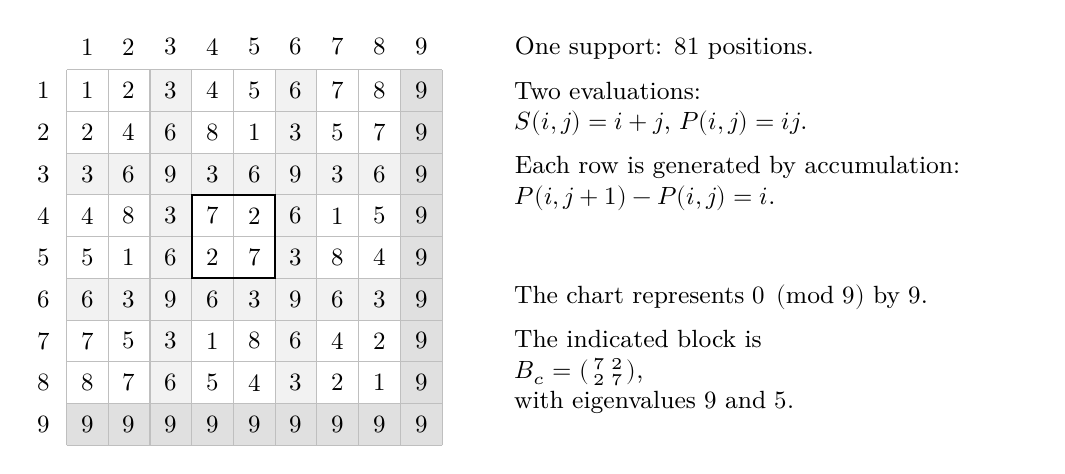
\begin{tikzpicture}[x=.53cm,y=.53cm,font=\small]
\fill[black!5] (1.5,-.5) rectangle (2.5,8.5);
\fill[black!5] (4.5,-.5) rectangle (5.5,8.5);
\fill[black!5] (-.5,2.5) rectangle (8.5,3.5);
\fill[black!5] (-.5,5.5) rectangle (8.5,6.5);
\fill[black!12] (7.5,-.5) rectangle (8.5,8.5);
\fill[black!12] (-.5,-.5) rectangle (8.5,.5);
\foreach \i in {1,...,9}{
 \node at (\i-1,9.05) {\(\i\)};
 \node at (-1.05,9-\i) {\(\i\)};
 \foreach \j in {1,...,9}{
  \pgfmathtruncatemacro{\v}{mod(\i*\j-1,9)+1}
  \node at (\j-1,9-\i) {\(\v\)};
 }
}
\foreach \k in {0,...,9}{
 \draw[black!25] (\k-.5,-.5)--(\k-.5,8.5);
 \draw[black!25] (-.5,\k-.5)--(8.5,\k-.5);
}
\draw[line width=.65pt] (2.5,3.5) rectangle (4.5,5.5);
\node[anchor=west,align=left,text width=6.5cm] at (10,7.2) {One support: \(81\) positions.\\[5pt]Two evaluations:\\ \(S(i,j)=i+j\), \(P(i,j)=ij\).\\[5pt]Each row is generated by accumulation:\\ \(P(i,j+1)-P(i,j)=i\).};
\node[anchor=west,align=left,text width=6.5cm] at (10,1.8) {The chart represents \(0\pmod9\) by \(9\).\\[5pt]The indicated block is\\ \(B_c=\left(\begin{smallmatrix}7&2\\2&7\end{smallmatrix}\right)\),\\ with eigenvalues \(9\) and \(5\).};
\end{tikzpicture}
\caption{Multiplication table of APP in positive representatives. Nonunit rows and columns are distinguished by gray shading; the frame identifies the adjacent diagonal block with equal diagonal entries. The displayed table is an observable of the arithmetic torus; its representational edges do not constitute an intrinsic topological boundary of the torus.}
\label{fig:app}
\end{figure}


\Needspace{12\baselineskip}
\begin{proposition}[Reconstruction of the evaluations]
The two pairs in \eqref{eq:app-levantada} determine \(i+j\) and \(ij\) exactly. The isolated residues do not determine those integer evaluations or their quotients.
\end{proposition}
\begin{proof}
The first assertion is \eqref{eq:residuo-cociente} applied to each sheet. For the second, \(10=1+9\) and \(19=1+2\cdot9\) have the same residue and different quotients. On the two-dimensional support, positions \((5,5)\) and \((8,2)\) give the same sum and the same product residue, but products \(25=7+18\) and \(16=7+9\). The residue projection identifies data that the lifted evaluation distinguishes.
\end{proof}

\subsubsection{Cayley graph, toroidal topology, and winding number}

In row and column coordinates, the cardinal translations are given by
\[
 \nu_N=(-1,0),\quad\nu_E=(0,1),\quad
 \nu_S=(1,0),\quad\nu_O=(0,-1),\qquad T_d(x)=x+\nu_d.
\]
The first coordinate increases southward and the second eastward. The graph
\[
 \mathscr G_9=\operatorname{Cay}(X_9,\{\nu_N,\nu_E,\nu_S,\nu_O\})
\]
is the two-dimensional cyclic lattice: it has eighty-one vertices and four outgoing oriented edges at each vertex. It is a Cayley graph for the \emph{additive} structure of the support. Residue multiplication has zero divisors and does not turn all APP rows into a multiplicative group.

A cardinal word \(w=d_1\cdots d_r\) and an origin \(x_0\) determine
\[
 x_k=x_0+\sum_{j=1}^k\nu_{d_j}\pmod9.
\]
There are \(81\cdot4^r\) oriented paths of length \(r\), including returns and backtracking. When the path closes, its integer displacement prior to reduction defines
\begin{equation}
 \operatorname{wind}(w)=\frac19
 \bigl(\#S(w)-\#N(w),\#E(w)-\#O(w)\bigr)\in\ZZ^2.
\end{equation}
Reversal of the path changes the sign of this vector. Return to the same residue position therefore does not force the winding to vanish. This is the first instance of a distinction that will recur in the phase return: one coordinate can close while another records a nontrivial evolution.

\subsubsection{Transport quotient and cocycle identity}

Let \(s_9:\ZZ/9\ZZ\to D_9\) be the section of positive representatives. The transport quotient associated with additive composition, also called the \emph{carry} in positional arithmetic, is
\[
 c_9(a,b)=\frac{s_9(a)+s_9(b)-s_9(a+b)}9.
\]
The compositional character of this memory is expressed by an exact identity.

\begin{lemma}[Cocycle identity]
For \(a,b,c\in\ZZ/9\ZZ\),
\[
 c_9(a,b)+c_9(a+b,c)=c_9(b,c)+c_9(a,b+c).
\]
\end{lemma}
\begin{proof}
Both sums are equal to
\[
 \frac{s_9(a)+s_9(b)+s_9(c)-s_9(a+b+c)}9.
\]
Associativity of the sum of lifted representatives requires precisely this additional term when composing in the quotient.
\end{proof}

With positive representatives, this cocycle is not normalized at the identity: \(c_9(0,a)=1\). If \(s_0\) takes representatives in \(\{0,\ldots,8\}\), its normalized carry \(c_0\) satisfies
\[
 c_9(a,b)=c_0(a,b)+\mathbf1_{a=0}+\mathbf1_{b=0}-\mathbf1_{a+b=0}.
\]
The difference is the change of section; it does not alter the cocycle identity. The later decomposition of the calendar into phase and window will use the representatives from zero through eight.

The totals of both evaluations distinguish the visible contribution from that preserved in the quotient:
\[
 \sum S=810,\quad\sum P=2025,\quad
 \sum\Sigma=405,\quad\sum\Pi=459,
\]
\[
 \sum q^+=45,\qquad\sum q^\times=174.
\]
It follows that
\begin{equation}
 2025-810=(459-405)+9(174-45)=54+9\cdot129.
 \label{eq:defecto-integrado}
\end{equation}
The sum--product difference is not exhausted by the visible defect \(54\). The identity also preserves the quotient defect \(129\). Suppressing it would change the arithmetic being transported, even if the residue table remained identical.

\subsubsection{Ternary reduction and multiplicative radical}

The ring \(R=\ZZ/9\ZZ\) has group of units \(\{1,2,4,5,7,8\}\) and maximal ideal
\[
 \mathfrak m=(3)=\{0,3,6\},\qquad\mathfrak m^2=0.
\]
Every additive row is a permutation of the nine representatives. A multiplicative row is such a permutation exactly when its index is a unit. Rows three and six contain three repeated values; row nine contains only the representative of the zero class. Thus, even before any continuous geometry, multiplicative folding distinguishes the units from the nilpotent sector.

The map \(x\mapsto3x\) has kernel and image both equal to \(\mathfrak m\). It induces an isomorphism of vector spaces over \(\FF_3\),
\[
 R/\mathfrak m\longrightarrow\mathfrak m,\qquad [x]\longmapsto3x,
\]
but not a ring isomorphism. In particular, the visible sequence \(3,6,9\) admits two different readings: its direct reduction modulo three is \(0,0,0\), whereas extracting the factor three and then reducing its internal coordinate gives \(1,2,0\). This second operation preserves a coordinate of the ideal; it is not the same projection as directly reducing the original number.

\subsubsection{Additive evaluation by means of a Latin square}

The difference between the two evaluations can also be expressed by means of
operators. Let \((e_r)_{r\in\ZZ/9\ZZ}\) be the orthonormal basis of \(\CC^9\).
The assignment \(v_{ab}=e_{a+b}\) produces an orthonormal basis in every row
and column. The projections \(P_{ab}=v_{ab}v_{ab}^{*}\) satisfy
\[
 \sum_bP_{ab}=I_9=\sum_aP_{ab},\qquad P_{ab}^2=P_{ab}.
\]
Indeed, every translation \(b\mapsto a+b\) permutes the nine residues.
This yields a realization of a Latin square by rank-one projections,
in the terminology of quantum Latin squares
\cite{mustovicary,delascuevas2023}. This construction starts from the
additive sheet already defined and makes explicit the map to its operator representation.

The multiplicative evaluation preserves different content: for \(a=3\), the
vectors \(e_{3b}\) repeat residues \(0,3,6\), and
\[
 \sum_{b\in\ZZ/9\ZZ}|e_{3b}\rangle\langle e_{3b}|
 =3\bigl(|e_0\rangle\langle e_0|+|e_3\rangle\langle e_3|
                    +|e_6\rangle\langle e_6|\bigr).
\]
Multiplicity is recorded in the operator and characterizes the multiplicative
radical. Consequently, the toroidal support, the Latin property, and the
operator resolution of the identity are properties that require
different definitions. The quantum magic squares studied by
De las Cuevas, Drescher, and Netzer require positive entries and row and column
sums equal to the identity; their theory also distinguishes
dilations with commuting entries\cite{delascuevas2020}. This reference
provides a precise language for comparing APP realizations.

\subsection{TRIT: orientation and quadratic regimes}

\begin{definition}[Ternary signature and local lift]
The TRIT signature uses the balanced identification
\[
 \FF_3\longrightarrow\TRIT,\qquad 0\mapsto0,\quad1\mapsto+1,\quad2\mapsto-1.
\]
For \(n\in\ZZ\), its lift preserves \(n=r+3c\), where \(r\in\TRIT\) and \(c\in\ZZ\). In a transition of bounded local amplitude, the three states \((0,-1),(0,0),(0,+1)\) can exhibit the same zero residue and different carries.
\end{definition}

The signature does not replace the path. A zero residue does not signify absence of orientation, phase, or quotient information. Nor does it introduce a physical magnitude by itself. Its function is to distinguish algebraically the transport classes to be realized next.

\subsubsection{Three quadratic regimes and a common exponential}

Once the ternary signature has been obtained, its quadratic realization is defined by
\begin{equation}
 \mathbb A_\tau=\RR[X]/(X^2+\tau),\qquad \tau\in\TRIT.
 \label{eq:algebras-trit}
\end{equation}
If \(J_\tau\) is the class of \(X\), then \(J_\tau^2=-\tau I\). The structure distinguishes the elliptic type \(\tau=+1\), the parabolic type \(\tau=0\), and the hyperbolic type \(\tau=-1\). The real realization does not generate the signature: it expresses the types already produced by the oriented reduction.

\begin{proposition}[Exponentiation of the three types]
In each algebra \eqref{eq:algebras-trit},
\begin{equation}
 \exp(tJ_\tau)=C_\tau(t)I+S_\tau(t)J_\tau,
\end{equation}
where
\[
 C_\tau(t)=\sum_{n\ge0}\frac{(-\tau)^nt^{2n}}{(2n)!},\qquad
 S_\tau(t)=\sum_{n\ge0}\frac{(-\tau)^nt^{2n+1}}{(2n+1)!}.
\]
The three realizations are
\[
 \begin{array}{c|c|c}
 \tau&J_\tau^2&\exp(tJ_\tau)\\\hline
 +1&-I&\cos t\,I+\sin t\,J_\tau\\
 0&0&I+tJ_\tau\\
 -1&I&\cosh t\,I+\sinh t\,J_\tau.
 \end{array}
\]
\end{proposition}
\begin{proof}
Separating the even and odd terms of the exponential series and substituting \(J_\tau^{2n}=(-\tau)^nI\) and \(J_\tau^{2n+1}=(-\tau)^nJ_\tau\) yields the formulas. For \(\tau=0\), all terms of degree at least two vanish. In the other two cases, the trigonometric or hyperbolic series are recovered.
\end{proof}

The exponential is common to all three regimes: it is not assigned exclusively to the parabolic branch. The invariants
\[
 C_\tau(t)^2+\tau S_\tau(t)^2=1
\]
follow from \(\exp(tJ_\tau)\exp(-tJ_\tau)=I\). The same algebraic principle preserves unity across realizations that differ in their quadratic type.

In the hyperbolic regime, \(P_\pm=(I\pm J_{-1})/2\) are complementary projections and
\[
 \exp(tJ_{-1})=e^tP_++e^{-t}P_-.
\]
Growth and contraction appear jointly along two eigendirections. In the elliptic regime, the parameter describes a rotation; in the parabolic regime, a nilpotent translation. The temporal interpretation adopted by HMT associates \(+1\) with return with memory, \(0\) with the threshold, and \(-1\) with bidirectional opening. This interpretation requires an order of parametrization; it does not add a fourth algebraic type.

% Cumulative expansion of TRIT; inserted before the regime figure.
% It neither replaces nor removes the preceding development.
\subsubsection{Balanced division and composition of the lifts}
\label{trit-ampl-div-balanceada}

Ternary reduction makes it possible to express an integer APP evaluation in a
visible coordinate and an extension coordinate. Its function is not
merely to abbreviate the notation of an integer: it provides a composition
rule that determines how the quotient changes when evaluations are added or
multiplied. The balanced choice also makes explicit the
compatibility of that rule with sign reversal.

\begin{definition}[Balanced ternary coordinates]
\label{trit-ampl-def-coordenadas}
For \(n\in\mathbb Z\), let
\[
 q_3(n)=\left\lfloor\frac{n+1}{3}\right\rfloor,\qquad
 r_3(n)=n-3q_3(n).
\]
The map
\[
 \mathcal B:\mathbb Z\longrightarrow\TRIT\times\mathbb Z,\qquad
 n\longmapsto(r_3(n),q_3(n))
\]
is called the balanced ternary decomposition. Its inverse is
\(\mathcal L(r,c)=r+3c\).
\end{definition}

Indeed, \(r_3(n)\in\{-1,0,+1\}\). If two pairs represent the same integer,
\(r+3c=s+3d\), then \(r-s\) is a multiple of \(3\) and lies in the interval
\([-2,2]\); necessarily \(r=s\) and \(c=d\). The representation is therefore
unique. Division can be repeated on \(q_3(n)\), so that each level
preserves the datum needed to reconstruct the preceding one. The quotient is not a
perturbation of the residue: it is its complementary coordinate.

The signature obtained from an evaluation \(F\), with \(F=S\) or \(F=P\) in APP,
is \(r_3\circ F\). When the reduction acts on the phase cursor, the same
balanced section produces the classes \(\{1,4,7\}\), \(\{2,5,8\}\), and
\(\{3,6,9\}\), with values \(+1,-1,0\). The TPK selector defined
below uses those classes to determine the operative mode.
Reading an evaluation and selecting a mode thus have the same
ternary reduction, but different domains and functions.

\Needspace{16\baselineskip}
\begin{proposition}[Arithmetic of balanced pairs]
\label{trit-ampl-prop-aritmetica}
Let \(n=r+3c\) and \(m=s+3d\), with \(r,s\in\TRIT\). Define
\[
 \chi(r,s)=\frac{r+s-r_3(r+s)}3.
\]
The integer operations are transported to the pairs by
\begin{align}
 (r,c)\boxplus(s,d)
 &=\bigl(r_3(r+s),c+d+\chi(r,s)\bigr),
 \label{trit-ampl-eq-suma}\\
 (r,c)\boxtimes(s,d)
 &=\bigl(rs,rd+sc+3cd\bigr).
 \label{trit-ampl-eq-producto}
\end{align}
The map \(\mathcal L\) preserves both operations.
\end{proposition}
\begin{proof}
The equality \(r+s=r_3(r+s)+3\chi(r,s)\) gives
\[
 n+m=r_3(r+s)+3\bigl(c+d+\chi(r,s)\bigr).
\]
On the other hand,
\[
 nm=rs+3(rd+sc+3cd).
\]
Since the product of two balanced representatives again belongs to
\(\{-1,0,+1\}\), it requires no additional residue reduction. Uniqueness
of the decomposition proves both formulas.
\end{proof}

For example, \(2=(-1)+3\) and \(4=1+3\). Their sum and product are reconstructed
as
\[
 (-1,1)\boxplus(1,1)=(0,2),\qquad
 (-1,1)\boxtimes(1,1)=(-1,3).
\]
The resulting evaluations are \(6\) and \(8\). The sum of quotients suffices
in this additive example; the product involves the cross terms
\(rd\), \(sc\), and \(3cd\). The discrepancy between the two operations also resides
in the extension coordinate, not only in the residue.

The term \(\chi\) is a cocycle of the balanced section. If
\(r\oplus s=r_3(r+s)\), it satisfies
\[
 \chi(r,s)+\chi(r\oplus s,t)
 =\chi(s,t)+\chi(r,s\oplus t).
\]
Both sides represent the quotient of the same sum of three integers.
This identity guarantees that regrouping the operations does not change the
reconstructed evaluation. At the same time, projection onto the first
component suppresses that accounting: \(1+1=-1+3\), whereas the residue
reading preserves only \(-1\). In this case, the information eliminated is
determined by \(\chi(1,1)=1\).

The relation with modulus \(9\) preserves a second discrete scale.
The map
\[
 \beta:\TRIT\times\mathbb F_3\longrightarrow\mathbb Z/9\mathbb Z,
 \qquad (r,\bar c)\longmapsto r+3c\pmod9
\]
is well defined and bijective. Changing the representative of \(\bar c\)
adds a multiple of \(9\); conversely, equality of images first fixes
\(r\) by reduction modulo \(3\) and then \(\bar c\). The sum
transported by this bijection contains the term
\(\chi(r,s)\) from \eqref{trit-ampl-eq-suma}, now reduced modulo \(3\).
Thus, the two ternary levels do not compose by an independent sum
of coordinates: normalization at the first level modifies
the second.

In particular, the classes \(3\), \(6\), and \(0\) in
\(\mathbb Z/9\mathbb Z\) have first component \(0\), but second
components \(1\), \(2\), and \(0\), respectively. The distinction already observed
between direct reduction and extraction of the ideal coordinate appears
as a property of \(\beta\). Preserving that coordinate prevents the
zero-residue sector from being artificially collapsed into a single position.
Modulus \(1000\), used later to organize decimal blocks,
serves a different positional-representation function; its quotient is preserved
through the corresponding division. A change of base preserves the integer
when it retains residue and quotient, whereas coincidence of residues
in different bases does not by itself identify their transport states.

\Needspace{11\baselineskip}
\subsubsection{Reversal, residue class, and nonvisible coordinates}
\label{trit-ampl-inversion}

Additive inversion lifts unambiguously:
\[
 \mathcal B(-n)=(-r_3(n),-q_3(n)).
\]
In particular, \(3\), \(0\), and \(-3\) have coordinates
\((0,1)\), \((0,0)\), and \((0,-1)\). They share the zero signature but represent
distinct evaluations. In a transition restricted to a quotient of
maximum amplitude \(1\), they are the three possibilities in the visible fiber over
zero; in a general integer lift, that fiber contains all pairs
\((0,c)\), with \(c\in\mathbb Z\).

The quotient coordinate recovers the evaluated integer, but does not by
itself recover the path that produced it. Two APP paths may share
evaluation, residue, and quotient, while differing in orientation, mode sequence, or
winding. The decomposition \(\mathcal B\) is therefore integrated into the
transport state rather than replacing it. The arithmetic memory of a
division and the memory of a path are related coordinates, not
synonyms.

For a sequence of signatures of length \(n\), the oriented reversal is
\[
 C_{\rm rev}(\tau_1,\ldots,\tau_n)
   =(-\tau_n,\ldots,-\tau_1).
\]
Applying it twice restores the sequence. The operation reverses the order of
the positions and the sign of each signature; it preserves the length and the
zero positions in reversed order. In the adopted parametrization, it
exchanges return with memory, associated with \(+1\), and bidirectional
opening, associated with \(-1\), while retaining the threshold \(0\). Transport
of the remaining path data is specified by the
corresponding TPK involution.

This reversal of signatures must be distinguished from conjugation within a
quadratic algebra. The former may change the type \(\tau\); the latter,
constructed below, acts within the type already fixed. The
distinction prevents attributing to sign reversal an algebraic equivalence
between different regimes.

\subsubsection{Quadratic product, conjugation, and algebraic norm}
\label{trit-ampl-norma}

An element of \(\mathbb A_\tau\) has a unique expression \(aI+bJ_\tau\).
The relation \(J_\tau^2=-\tau I\) determines its product:
\begin{equation}
 (aI+bJ_\tau)(cI+dJ_\tau)
   =(ac-\tau bd)I+(ad+bc)J_\tau.
 \label{trit-ampl-producto-cuadratico}
\end{equation}
This is a real realization of the type already selected. The coordinates
\(a,b\) are not APP residues, and product
\eqref{trit-ampl-producto-cuadratico} does not replace
\eqref{trit-ampl-eq-producto}; it expresses a different operation in the stated
quadratic codomain.

\begin{definition}[Conjugation and algebraic norm]
\label{trit-ampl-def-norma}
Conjugation of type \(\tau\) and its algebraic norm are
\[
 \overline{aI+bJ_\tau}=aI-bJ_\tau,\qquad
 N_\tau(aI+bJ_\tau)=a^2+\tau b^2.
\]
\end{definition}

\begin{proposition}[Multiplicativity and invertibility]
\label{trit-ampl-prop-norma}
For \(z,w\in\mathbb A_\tau\),
\[
 z\bar z=N_\tau(z)I,\qquad
 N_\tau(zw)=N_\tau(z)N_\tau(w).
\]
Moreover, \(z\) is invertible if and only if \(N_\tau(z)\ne0\), and in that case
\[
 z^{-1}=\frac{\bar z}{N_\tau(z)}.
\]
\end{proposition}
\begin{proof}
The product of \(aI+bJ_\tau\) and \(aI-bJ_\tau\) is
\((a^2+\tau b^2)I\). Conjugation is multiplicative and the algebra is
commutative, so
\((zw)\overline{zw}=(z\bar z)(w\bar w)\). If the norm does not vanish, the
stated formula provides the inverse. Conversely, if \(zw=I\),
multiplicativity implies \(N_\tau(z)N_\tau(w)=1\).
\end{proof}

The quadratic form \(N_\tau\) is positive definite only in the elliptic type.
For \(\tau=0\), it equals \(a^2\), and the element \(J_0\) is nonzero even though its
square and norm are zero. For \(\tau=-1\), it equals \(a^2-b^2\); the
nonzero elements \(I+J_{-1}\) and \(I-J_{-1}\) have zero norm and their
product vanishes. Here the algebraic norm is a multiplicative quadratic
form: it does not presuppose a positive vector-space norm.

The three types can be faithfully realized by
\[
 aI+bJ_\tau\longmapsto
 \begin{pmatrix}a&-\tau b\\b&a\end{pmatrix}.
\]
The determinant of this matrix is \(N_\tau(aI+bJ_\tau)\). Thus, by a
single matrix expression, it represents the complex structure, the
dual-number structure, and the split-real structure.
Each preserves its law and its zero divisors. The signature-\((1,1)\)
form in the last case has a Lorentzian interpretation in dimension
\(1+1\); identifying a physical metric additionally requires a specific space,
field, and transport rule.

\subsubsection{Multiplicative conservation and composition of evolutions}
\label{trit-ampl-evoluciones}

The exponential already obtained belongs to the set of elements of norm one:
\[
 N_\tau\bigl(\exp(tJ_\tau)\bigr)=1.
\]
This conservation is maintained under composition of parameters. Indeed, all
factors are functions of the same generator, and
\[
 \exp(tJ_\tau)\exp(sJ_\tau)=\exp((t+s)J_\tau).
\]
Comparison of the two components yields the addition laws
\begin{align}
 C_\tau(t+s)&=C_\tau(t)C_\tau(s)-\tau S_\tau(t)S_\tau(s),\\
 S_\tau(t+s)&=S_\tau(t)C_\tau(s)+C_\tau(t)S_\tau(s).
\end{align}
Conjugation changes \(t\) to \(-t\) and coincides with inversion within
this subgroup. It does not change \(\tau\): it reverses an evolution in the
selected regime.

In the elliptic type, the preserved form is \(a^2+b^2\), and the exponential
path traverses the unit circle. In the hyperbolic type, the
eigencoordinates are \(u=a+b\), \(v=a-b\), with \(uv=N_{-1}(z)\).
The exponential gives
\[
 (u,v)=(e^t,e^{-t}),\qquad uv=1.
\]
Growth of one coordinate is accompanied by contraction of the other.
Conservation expresses a relation between both coordinates; it does not assert that
each remains constant.

In the parabolic type,
\[
 (I+tJ_0)(I+sJ_0)=I+(t+s)J_0,\qquad
 (I+tJ_0)^{-1}=I-tJ_0.
\]
Evolution does not stop because \(J_0^2=0\). Nilpotence eliminates
terms of order at least two but preserves the linear term that
transports the parameter. The visible symbol \(0\), the zero element of the
algebra, and the nonzero generator \(J_0\) are distinct. This distinction
is necessary to describe the threshold without identifying it with absence of
state or dynamics.

\begin{proposition}[Composition of affine coordinates]
\label{trit-ampl-prop-pendientes}
In the chart where the scalar component does not vanish, represent a
direction by \(I+uJ_\tau\). If \(1-\tau uv\ne0\), the direction of its
product with \(I+vJ_\tau\) has coordinate
\[
 u\star_\tau v=\frac{u+v}{1-\tau uv}.
\]
\end{proposition}
\begin{proof}
We have
\[
 (I+uJ_\tau)(I+vJ_\tau)
   =(1-\tau uv)I+(u+v)J_\tau.
\]
Dividing by the scalar component gives the stated expression.
\end{proof}

The affine chart preserves the ratio between components, not the divided-out
scalar factor. When \(1-\tau uv=0\), the product must be examined before
changing charts: it may have a defined direction with zero scalar component,
or be the zero element in the presence of zero divisors. The composition
law remains part of the complete algebra; singularity of a coordinate does not
automatically imply singularity of the object.
This formula will reappear in the elliptic regional reading. Its use requires
retaining the denominator and, where applicable, the normalization factor.

\subsubsection{Transport of type and subsequent realizations}
\label{trit-ampl-puentes}

The algebras \(\mathbb A_{+1}\), \(\mathbb A_0\), and
\(\mathbb A_{-1}\) are not isomorphic as unital real algebras.
The first is a field; the second contains a nonzero nilpotent; the
third has nontrivial idempotents and is isomorphic to
\(\mathbb R\times\mathbb R\). Therefore, the signature change that organizes a
route cannot be interpreted as an undifferentiated isomorphism among the
three realizations. The TPK preserves the regime index, the domains, and the
effective operator acting at each transition.

Within the electronic chapter, the pair of projections from the APP sheets
produces a normalized commutator whose square is \(-I\). The same block
contains an involution with square \(I\) and two nilpotent directions. The
joint realization will be proved on that specific pair of projections;
the preceding classification explains why the three quadratic relations
can appear in the same matrix algebra without being identified with one another.

In the exceptional extension, the Paley matrix reduced modulo \(3\)
satisfies \(A_W^2=-I_6\). This relation endows the ternary space with a
structure of dimension \(3\) over \(\mathbb F_9\). Its link with a real
operator root is expressed through the integral presentation
\[
 \mathbb Z[u]/(u^2+1).
\]
Base changes to \(\mathbb F_3\) and \(\mathbb R\) produce
representations of that same relation. Each preserves its characteristic,
dimension, and incidence information. Development of the
respective operators establishes the link, not equality of their
cardinalities.

Preservation of norm one consequently describes the quadratic
realizations of the evolutions. Preservation of quotients, orientation, and
path belongs to the transported arithmetic state. Both properties
enter the construction with different functions: one determines the
identities of the representations; the other makes it possible to compose, reconstruct, and
extend the operations that originate them.


\begin{figure}[htbp]
\centering
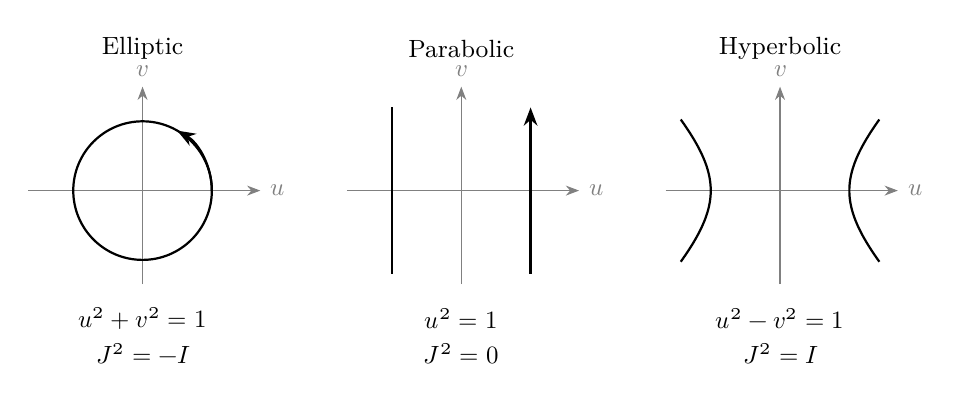
\begin{tikzpicture}[scale=.88,>=Stealth,font=\small]
\foreach \c/\titulo in {0/{Elliptic},4.6/{Parabolic},9.2/{Hyperbolic}}{
\begin{scope}[xshift=\c cm]
\draw[->,gray] (-1.65,0)--(1.7,0) node[right] {\(u\)};
\draw[->,gray] (0,-1.35)--(0,1.5) node[above] {\(v\)};
\node at (0,2.05) {\titulo};
\end{scope}}
\draw[thick] (0,0) circle[radius=1];
\draw[->,thick] (1,0) arc[start angle=0,end angle=60,radius=1];
\node at (0,-1.85) {\(u^2+v^2=1\)};
\node at (0,-2.35) {\(J^2=-I\)};
\draw[thick] (3.6,-1.2)--(3.6,1.2);
\draw[->,thick] (5.6,-1.2)--(5.6,1.2);
\node at (4.6,-1.85) {\(u^2=1\)};
\node at (4.6,-2.35) {\(J^2=0\)};
\draw[thick,domain=-.9:.9,samples=50] plot ({9.2+cosh(\x)},{sinh(\x)});
\draw[thick,domain=-.9:.9,samples=50] plot ({9.2-cosh(\x)},{sinh(\x)});
\node at (9.2,-1.85) {\(u^2-v^2=1\)};
\node at (9.2,-2.35) {\(J^2=I\)};
\end{tikzpicture}
\caption{Quadratic realizations of TRIT. For
\(J_\tau=\left(\begin{smallmatrix}0&-\tau\\1&0\end{smallmatrix}\right)\),
the exponential preserves \(u^2+\tau v^2\). The parabolic degeneration
preserves \(u\) and transports \(v\) linearly. The three diagrams represent
orbits of quadratic forms; their geometric type corresponds to the algebraic
relation of the generator.}
\label{fig:trit-regimenes}
\end{figure}


\subsection{TPK: topological phase kernel}

The dynamics uses the phase selector
\[
 M_{\rm ph}(r)=
 \begin{cases}
 +1,&r\in\{1,4,7\},\\
 -1,&r\in\{2,5,8\},\\
 0,&r\in\{3,6,9\}.
 \end{cases}
\]
Its value determines which evaluation operates. Cardinal transport moves the corresponding cursor; the record preserves the previous value, the new quotient, the orientation, and the transition. Selection and transport are therefore distinct functions: a ternary sign is not a displacement on the torus.

We denote by \(\widehat X\) the space of arithmetic states with path memory. An element contains the positions and directions of both cursors, the active mode, the TRIT signature, the phase, the residues and quotients of both evaluations, the carries, the constructed prefix, and the boundary data. When a refinement cylinder is introduced, it forms part of the state. This notation prevents replacement of the object by a reduced version that preserves only the visible symbol.

\begin{definition}[TPK update]
Let \(\mathsf{Sel}_t\) be mode selection through \(M_{\rm ph}\), \(\mathsf{Tra}_t\) the lifted cardinal transport, and \(\mathsf{Mem}_t\) the update of the records. The transition is
\begin{equation}
 \mathcal U_t=\mathsf{Mem}_t\circ\mathsf{Tra}_t\circ\mathsf{Sel}_t.
 \label{eq:actualizacion}
\end{equation}
Each map preserves the fields it does not modify and updates the remaining ones by Euclidean division and path concatenation.
\end{definition}

The notation \eqref{eq:actualizacion} expresses the order of composition; it does not
replace the effective rules. The two-cursor recurrence of
Section~\ref{sec:extension} completely specifies this finite realization.
Thereafter, extension will not be obtained by erasing its memory and repeating the
first emission, but by transporting the prefixes and their compatible boundaries.
In this way, APP provides the evaluations, TRIT distinguishes their regimes,
and TPK composes their evolution.

% Expository recovery from the owners of the TPK core.
% Provenance and preservation control are documented in technical/TPK_INTEGRACION.md.
% This file expands the TPK section; it does not replace extension.tex or generacion.tex.

\subsubsection{Dynamical state, observables, and dependence of the operations}
\label{tpk-int:estado}

The topological phase kernel organizes the evolution of the two APP sheets
with the orientation determined by TRIT. Its definition comprises the state
on which it acts, the transition rules, and the relations that make
extensions compatible. Equation \eqref{eq:actualizacion} acquires
operational content by specifying which coordinates each of its factors receives
and modifies. Position belongs to the toroidal support; phase
belongs to the calendar; orientation determines transport; the
quotients record the arithmetic evaluation prior to its reduction.
These coordinates are related through the transition and retain distinct
mathematical functions.

The observable projection of a state is
\begin{equation}
 q=(x_+,d_+,x_\times,d_\times,\theta)
 \in\mathcal Q_{\rm obs}
 :=(X_9\times\mathcal D)^2\times\Theta_{108},
 \qquad \mathcal D=\{N,E,S,O\},\quad
 \Theta_{108}=\ZZ/108\ZZ.
 \label{tpk-int:qobs}
\end{equation}
The subscripts distinguish the additive and multiplicative cursors. In the
fibers of complete states over \(q\), the ordered path, the integer evaluations
of both sheets, their residues and quotients, and the orientation and boundary
records are preserved. A precision extension adds the
prefix and the compatible cylinder. Thus, two states with the same
projection \(q\) may preserve different records.

The dependence of the operations has three levels. At the local level,
the selector activates a sheet, transport modifies its position, and the
update calculates the new arithmetic coordinates. At the path level,
these transitions compose and preserve the records of
preceding steps. At the refinement level, extension relations
determine which continuation preserves the prefix, signature, and
boundary of the antecedent. The finite calendar describes the phase of those
operations; holonomy describes their composition on the history.

\subsubsection{Tritic selection and lifted cardinal transport}
\label{tpk-int:seleccion}

Let \(\bar\theta\in\{0,\ldots,107\}\) be the calendar representative.
The operative phase and the dodecaphase sector are
\begin{equation}
 r(\theta)=1+(\bar\theta\bmod9),\qquad
 \beta(\theta)=\left[\left\lfloor\frac{\bar\theta}{9}\right\rfloor\right]_{12}.
 \label{tpk-int:fase}
\end{equation}
The selector already defined can be written \(\varepsilon_9=M_{\rm ph}\).
Its value vector, in the ordered chart of \(D_9\), is
\[
 m_{\rm ph}=(1,-1,0,1,-1,0,1,-1,0).
\]
The function \(M_{\rm ph}:D_9\to\TRIT\) and this vector are two
presentations of the same selector, with their respective domains.

Define the activation indicators
\[
 a_+(\theta)=\mathbf1_{\{1,4,7\}}(r(\theta)),\qquad
 a_\times(\theta)=\mathbf1_{\{2,5,8\}}(r(\theta)).
\]
The cursor transport is then
\begin{equation}
 x_+'=x_++a_+(\theta)\nu_{d_+},\qquad
 x_\times'=x_\times+a_\times(\theta)\nu_{d_\times}
 \quad\text{in }X_9.
 \label{tpk-int:cursores}
\end{equation}
At phases \(3,6,9\), both positions remain fixed; the neutral event
forms part of the chronology and its record. The cardinal directions
determine the vectors \(\nu_d\), while the phase signature determines
which of those vectors is applied.

The integer lift preserves the boundary crossing. If
\(s:X_9\to D_9^2\) selects the positive representatives and
\(x'=x+a\nu_d\), with \(a\in\{0,1\}\), define
\begin{equation}
 b_d(x,a)=\frac{s(x)+a\nu_d-s(x')}{9}\in\ZZ^2.
 \label{tpk-int:borde}
\end{equation}
Divisibility by \(9\) follows from equality in \(X_9\).
If \(z\in\ZZ^2\) records the preceding crossings, the update is
\(z'=z+b_d(x,a)\). Thus,
\[
 s(x')+9z'=s(x)+9z+a\nu_d.
\]
The integer transport datum remains reconstructible after the
position on the torus is reduced.

\begin{proposition}[Preservation of the lifted displacement]
\label{tpk-int:prop-desplazamiento}
For a cardinal path of \(n\) steps, whose activation indicators
are \(a_t\),
\[
 s(x_n)+9z_n=s(x_0)+9z_0+
 \sum_{t=0}^{n-1}a_t\nu_{d_t}.
\]
The same equality is preserved when two compatible paths are concatenated.
\end{proposition}
\begin{proof}
The one-step identity is \eqref{tpk-int:borde}. Summing it over the
\(n\) steps cancels the intermediate coordinates. Dividing the summation
range into two segments produces exactly the concatenation law. For a
closed path, the difference \(z_n-z_0\) is the previously defined
winding number.
\end{proof}

The same principle governs the APP evaluations. If a sheet takes the
integer value \(N_t\), its record simultaneously preserves
\(N_t=R_t+9q_t\). The difference between two steps satisfies
\[
 N_{t+1}-N_t=(R_{t+1}-R_t)+9(q_{t+1}-q_t).
\]
The spatial-crossing memory \(z_t\) and the arithmetic quotient \(q_t\)
have different definitions; their joint preservation maintains the
geometric and arithmetic provenance of each transition.

\subsubsection{Two-cursor chronology and composite returns}
\label{tpk-int:cronologia}

The cardinal involution \(\jmath\) exchanges \(N\) with \(S\) and
\(E\) with \(O\). After applying \eqref{tpk-int:cursores}, both
directions are reversed when a block of \(27\) steps ends.
Writing
\[
 h(\theta)=\mathbf1_{\{0,27,54,81\}}
             ((\bar\theta+1)\bmod108),
\]
the complete rule on the observable projection is
\begin{equation}
 F_{\rm obs}(q)=
 \bigl(x_+',\jmath^{h(\theta)}d_+,
       x_\times',\jmath^{h(\theta)}d_\times,
       \theta+1\bigr).
 \label{tpk-int:fobs}
\end{equation}
The reading that forms the emission uses the positions prior to
transport, according to the explicit recurrence of
Section~\ref{sec:extension}. The observable update and the emission
therefore compose in a fixed order.

\begin{proposition}[Reversibility and period of the observable calendar]
\label{tpk-int:periodo}
The map \(F_{\rm obs}\) is a permutation of
\(\mathcal Q_{\rm obs}\) and satisfies \(F_{\rm obs}^{108}=I\).
In a block of \(54\) steps, positions and directions are restored;
the \(\Theta_{108}\) coordinate advances by \(54\).
\end{proposition}
\begin{proof}
Given the final state, the preceding phase is first recovered by subtracting one
in \(\Theta_{108}\). That phase determines whether the directions were
reversed and which cursor was displaced. Applying the corresponding involution
and subtracting the cardinal vector uniquely recovers the initial state.

Each interval of \(27\) steps contains nine activations of each
cursor. The following block preserves the activations and reverses the
directions, so the integer displacements cancel over
\(54\) steps. The rule has period \(54\) in its position and
orientation increments; the same cancellation holds for any calendar
origin. After \(108\) steps, \(\theta\) is also restored.
\end{proof}

Set aside
\[
 \mathcal K_{27}=F_{\rm obs}^{27}:
 \mathcal Q_{\rm obs}\longrightarrow\mathcal Q_{\rm obs}
\]
for the iterate of \(27\) transitions. Its fourth iterate is the
identity on the observable state defined in \eqref{tpk-int:qobs}.
Projection of the history to the calendar permits this finite
verification. The path record, its evaluations, and
the new prefixes are preserved in the dynamical state on which
\(\mathcal U_t\) acts; observable equality does not reinitialize them.

\subsubsection{Affine transport of memory and composition of states}
\label{tpk-int:memoria}

The observable projection admits fibers of arithmetic and geometric data.
Over a configuration \(q\), write a state in the form
\[
 x=(q,o,h,c,\sigma,C,b,\lambda).
\]
Here \(o\) preserves the orientation and the sheet; \(h\), the residues
and quotients; \(c\), the additive transport memory; \(\sigma\),
the boundary signature; \(C\), the precision cylinder; \(b\), its
boundary label; and \(\lambda\), the recorded path. The
signature is determined by a map
\[
 \operatorname{Sig}_q:
 \mathsf H_q\times\mathsf C_q\times\mathsf{Hist}_q
 \longrightarrow\mathsf S_q,
 \qquad \sigma=\operatorname{Sig}_q(h,c,\lambda).
\]
The symbols \(\mathsf H_q,\mathsf C_q,\mathsf{Hist}_q\), and
\(\mathsf S_q\) denote, respectively, the sets of residue--quotient data,
the abelian group of transport memory, the
recorded paths, and the boundary signatures.
Realizations of this signature are specified componentwise in
the regional and terminal constructions. This dependence prevents treating
the signature as a free parameter once the data that produce it have been fixed.

The elementary residue-and-quotient chart is explicit. For
\(n\in\ZZ\), let
\[
 r=1+((n-1)\bmod9),\qquad u=\frac{n-r}{9}.
\]
Then \(n=r+9u\), with \(r\in D_9\) and \(u\in\ZZ\).
Uniqueness follows because two representatives of \(D_9\) congruent
modulo \(9\) are equal. This chart provides the local integer
reconstruction. The precision towers also incorporate the truncation maps
and the cylinders developed in
\ref{sec:extension} and \ref{sec:generacion}.

Let \(\gamma:q\to q'\) be an observable path. Transport
of the fibers is expressed by maps
\[
 \mathsf H(\gamma):\mathsf H_q\to\mathsf H_{q'},\qquad
 \mathsf C(\gamma):\mathsf C_q\to\mathsf C_{q'},\qquad
 \mathsf{Hist}(\gamma):\mathsf{Hist}_q\to\mathsf{Hist}_{q'}.
\]
The maps respect identities and composition, and
\(\mathsf C(\gamma)\) is a homomorphism of abelian groups.
The increment \(k_{\rm tr}(\gamma)\in\mathsf C_{q'}\) satisfies
\begin{equation}
 \begin{split}
 k_{\rm tr}(\operatorname{id}_q)&=0,\\
 k_{\rm tr}(\gamma_2\circ\gamma_1)
 &=k_{\rm tr}(\gamma_2)+
   \mathsf C(\gamma_2)k_{\rm tr}(\gamma_1).
 \end{split}
 \label{tpk-int:cociclo}
\end{equation}
Here the symbol \(k_{\rm tr}\) denotes the transport cocycle;
the rational coordinate \(\kappa\) of record \(K\) retains
its notation in the chapter on dodecaphase closure.

The transportable coordinates are updated by
\begin{equation}
 \begin{aligned}
 h'&=\mathsf H(\gamma)h,&
 c'&=\mathsf C(\gamma)c+k_{\rm tr}(\gamma),\\
 \lambda'&=\gamma\circ\lambda,&
 \sigma'&=\operatorname{Sig}_{q'}(h',c',\lambda').
 \end{aligned}
 \label{tpk-int:accion-memoria}
\end{equation}
The second equation is an affine action: the linear term transports
the preceding memory, and the cocycle adds the increment produced by the
path. In the spatial-crossing realization of each cursor separately,
\(\mathsf C(\gamma)=I\), and \(k_{\rm tr}(\gamma)\) is the sum
of the vectors in \eqref{tpk-int:borde}. This concrete instance
links the abstract law with the cardinal operations already defined.

\begin{proposition}[Compatibility of the update with concatenation]
\label{tpk-int:composicion-memoria}
Update \eqref{tpk-int:accion-memoria} by
\(\gamma_1\), followed by update by \(\gamma_2\),
coincides with update by \(\gamma_2\circ\gamma_1\).
\end{proposition}
\begin{proof}
For the affine coordinate, two updates give
\[
 c''=\mathsf C(\gamma_2)\mathsf C(\gamma_1)c
       +\mathsf C(\gamma_2)k_{\rm tr}(\gamma_1)
       +k_{\rm tr}(\gamma_2).
\]
Functoriality of \(\mathsf C\) and
\eqref{tpk-int:cociclo} turn this expression into
\(\mathsf C(\gamma_2\circ\gamma_1)c+
k_{\rm tr}(\gamma_2\circ\gamma_1)\).
The assertion for \(h\) follows from composition of
\(\mathsf H\), and that for \(\lambda\) from associativity of
paths. The final signature coincides because it is evaluated on the same
three reconstructed coordinates.
\end{proof}

The cylinder and its boundary complete this law through the relations
\(\operatorname{Ext}_\gamma\), defined in
\ref{tpk-int:bidireccionalidad}. Their elements determine which of
the preceding updates preserve an admissible extension.
The states, together with the triples \((\gamma,x,x')\) admitted by
those relations, form a category over the observable paths:
\[
 (\gamma_2,x',x'')\circ(\gamma_1,x,x')
     =(\gamma_2\circ\gamma_1,x,x'').
\]
The identity of \(x\) is \((\operatorname{id}_q,x,x)\).
Composition simultaneously preserves arithmetic transport and
boundary extendability. This is the structure in which
returns with memory and successive refinements are effected.

\subsubsection{Dodecaphasic record, phase, and accumulated memory}
\label{tpk-int:dodecafase}

The \(108\) transitions are distributed among the ordered windows
\[
 E_m=\{9m-8,\ldots,9m\},\qquad 1\leq m\leq12.
\]
The record preserves the phase origin, orientation, and data
produced during each window. Its map is
\[
 \mathcal R_{12}(x)=
 \bigl((E_m,\tau_m,\sigma_m,\kappa_m,\Lambda_m)\bigr)_{m=1}^{12},
\]
where \(\tau_m\) is the subroute in the window, \(\sigma_m\) its
orientation, \(\kappa_m\) the integer boundary increment, and
\(\Lambda_m\) the local incidence record. We adopt the chart
to be developed in \ref{subsec:k-registro-integral}; its window indices
correspond to \(m=\beta+1\).
The domain comprises the compatible TPK histories, and the codomain their
oriented temporal records. Composition of segments and their increments
is governed by \eqref{tpk-int:accion-memoria}. The group \(C_{12}\), by
contrast, describes translation of the window index; \(\Theta_{108}\) preserves
the step calendar. This distinction specifies what is transformed
and what is observed upon completion of a cycle.

In coordinates \(\theta=9b+r\), with \(0\leq r<9\), advancing
\(9\) steps preserves \(r\) and increases \(b\) by one.
Addition of phases introduces the quotient
\[
 c_0(r,r')=\left\lfloor\frac{r+r'}9\right\rfloor,
\]
whose cocycle identity ensures associativity of composition.
The finite calendar preserves \([b]_{12}\); a record of
circuits preserves \(b\in\ZZ\), or \(b\in\mathbb N_0\) for
a history with fixed origin. Section~\ref{sec:extension} proves
the nonsplit exact sequence \eqref{eq:extension108}. Its function is
to describe the relation between these coordinates before using them in the
construction of the signed state.

The signed record receives the phase and memory data through the
composition developed in Section~\ref{sec:k-registro}; on the
compatible sublattice, the notations \(\mathcal S_{12}\) and
\(R_{\mathrm{sgn}}\) denote the same reader:
\begin{equation}
 \mathcal S_{12}\equiv R_{\mathrm{sgn}}
 =\Pi_H\circ\mathcal E_{108}^{90,120}
                         \circ\mathcal R_{12}.
 \label{tpk-int:registro-causal}
\end{equation}
Its domain is the terminal state with memory; its output belongs to
\(\ZZ^{12}\). The reversible transformation between that signed state
and \(K\), as well as the rational reading of \(K\), are proved in
the corresponding chapter. The recording operations precede
those transformations. Reconstruction of a record from its cyclic
differences verifies its recoverability; the dynamical provenance
must be preserved through the events that produced it.
Equation~\eqref{tpk-int:registro-causal} fixes the type and effective
composition. The terminal state is produced by the one hundred eight updates
\(\mathcal U_t=\mathsf{Upd}_t\circ\mathsf{Tra}_t\circ\mathsf{Sel}_t\);
\(\mathcal R_{12}\) preserves the twelve windows with orientation, carry,
boundary, and ledger, and \(\mathcal E_{108}^{90,120}\) expresses the channels
\((b^{90},b^{120},Q_{\rm TPK})\). Section~\ref{sec:k-registro}
incorporates the exact evaluation and proves that
\(\Pi_H\) produces \(U_{\rm term}\) before the Hadamard inversion that
produces \(K\). The focal verifier deliberately begins at the channel
coordinate to check the subsequent chart and its return focally and exactly;
the scope of that auxiliary program is not confused with the scope of
the mathematical construction.

For the coded trace \((d_t)\) preserved by the record, the
event reader counts codes \(\{2,4,6,8\}\) in each
window with orientation
\((+,+,+,-,-,-,+,+,+,-,-,-)\). These codes and the cardinal
symbols in \(\mathcal D\) are distinct coordinates of the
record. Chapter~\ref{sec:k-registro} develops this reader,
the integral decomposition \(1+5+6\), the congruences that
characterize its image, and its exact inverse. The inversion proof
establishes which data that chart preserves; the definition of
\(\mathcal R_{12}\) specifies the oriented history on which it
acts.

\subsubsection{Phase incidence and internal construction of the channels}
\label{tpk-int:incidencia}

The selector determines three subsets of \(D_9\):
\[
 H_+=\{1,4,7\},\qquad H_-=\{2,5,8\},\qquad H_0=\{3,6,9\}.
\]
Let \(H_{\rm act}=H_+\sqcup H_-\) be the set of active phases and
let \(O_{\rm ph}=D_9\setminus\{9\}\) be the chart preceding the marked
return. Denote by \(P_2(H_{\rm act})\) the set of unordered pairs
of active phases. The internal incidence is given by
\begin{equation}
 \mathcal F^{\rm ph}_6=H_{\rm act}\times P_2(H_{\rm act}),\qquad
 \mathcal F^{\rm ph}_8=O_{\rm ph}\times P_2(H_{\rm act}),\qquad
 \Theta_{\rm ph}=D_9\times P_2(H_{\rm act}).
 \label{tpk-int:fases90120}
\end{equation}
The indices describe the number of positions in the first component.
The construction uses the phases and calendar origin already fixed;
the subsequent exceptional realizations will transport these
incidences to their own domains.

\begin{proposition}[Cardinalities and oriented phase incidence]
\label{tpk-int:cardinales}
The sets in \eqref{tpk-int:fases90120} have cardinalities
\(90,120,135\), respectively. If
\[
 \partial_{\rm ph}=\Theta_{\rm ph}\times\{-1,+1\},\qquad
 E_{\rm ph}=\partial_{\rm ph}\sqcup\{\infty\},\qquad
 L_{\rm ph}=H_0\times P_2(H_{\rm act}),
\]
then
\[
 |\partial_{\rm ph}|=270,\quad |E_{\rm ph}|=271,\quad
 |L_{\rm ph}|=45,\quad
 |\partial_{\rm ph}\sqcup L_{\rm ph}|=315.
\]
Simultaneously translating the phase origin and the marked return preserves
all these cardinalities and their inclusions.
\end{proposition}
\begin{proof}
There are six active phases, so
\(|P_2(H_{\rm act})|=\binom62=15\). Multiplication by
\(6,8,9\) gives \(90,120,135\). Orientation doubles \(135\);
the return mark adds one element; the three neutral phases give
\(3\cdot15=45\). A calendar translation transports each
factor by a bijection and takes the marked point to its image. Products
and disjoint unions thus preserve incidence.
\end{proof}

Here the cardinality \(271\) has a realization by phase incidence.
The cubic completion of Section~\ref{sec:extension} has
its own construction of the shell \(1000-729\). The correspondence
between the two realizations must preserve the maps and marks that
identify them, in addition to the cardinality. Likewise, the selector
\(\varepsilon_9\), the incidence \((90,120)\), and the extractor
\(\mathcal E_{108}^{90,120}\) preserve the domains and operations
just distinguished.

\subsubsection{Path reversal and conjugate extensions}
\label{tpk-int:bidireccionalidad}

Bidirectionality begins with an operation on paths, before
scalar values are assigned to them. For
\(\gamma=(x_0;d_1,\ldots,d_n)\), with endpoint \(x_n\), define
\[
 \operatorname{rev}\gamma
   =(x_n;\jmath d_n,\ldots,\jmath d_1).
\]
The origin of the reversed path is the endpoint of the original.
Composition satisfies
\[
 \operatorname{rev}^2\gamma=\gamma,\qquad
 \operatorname{rev}(\gamma_2\circ\gamma_1)
   =\operatorname{rev}\gamma_1\circ\operatorname{rev}\gamma_2,
\]
and the integer displacement changes sign. These identities are obtained
by reversing the order of the steps and replacing each cardinal vector by
its opposite. For a loop it follows that
\(\operatorname{wind}(\operatorname{rev}\gamma)
=-\operatorname{wind}(\gamma)\).

On the records, reversal also requires transporting the order
of their components and the orientation of their events. Route reversal
and signature conjugation are distinguishable operations: their
composition is specified when applied to a particular record. In
particular, the regional involution that exchanges the closure and
propagation components preserves the self-scaling axis; its formula is
presented in Section~\ref{mono-ampl:regiones}. This regional operation
acts on a domain different from reversal of a cardinal path.

Extensions along a route \(r:q\to q'\) are expressed by
relations between fibers of compatible states. If \(\mathcal F_q\)
denotes the fiber of complete states over \(q\), require
\[
 \operatorname{Ext}_r\subseteq\mathcal F_q\times\mathcal F_{q'},
 \qquad \Delta_{\mathcal F_q}\subseteq
        \operatorname{Ext}_{\operatorname{id}_q},
\]
\[
 \operatorname{Ext}_{r_2}\circ\operatorname{Ext}_{r_1}
       \subseteq\operatorname{Ext}_{r_2\circ r_1}.
\]
Their composition preserves the evaluations of both sheets, the orientation,
the quotients, the prefix, and the boundary. Reversal of the route does not
by itself imply that every extension relation is a bijection.
The conjugate extension is defined on the domain where transport of
those data satisfies the corresponding compatibilities.

\subsubsection{Nonadic holonomy and continuity of refinement}
\label{tpk-int:holonomia}

One phase circuit composes the transitions on the state with memory:
\begin{equation}
 \Gamma_{9,k}=\mathcal U_{k+8}\circ\cdots\circ\mathcal U_k.
 \label{tpk-int:gamma}
\end{equation}
On an individualized history, this functional composition realizes
the holonomy relation; on the complete domain,
\(\Gamma_{9,k}\subseteq\widehat X_k\times\widehat X_{k+9}\) is preserved,
with admissible extensions developed below.
The cyclic base has nine phases, while
the fiber preserves the path, quotients, and boundary.
Monodromy is the action of one circuit of that base on the fibers; the
holonomy \(\Gamma_{9,k}\) expresses its realization by the effective
TPK transitions.

If \(g\) observes the phase and \(M\) the number of preserved circuits,
\[
 g(\Gamma_{9,k}x)=g(x),\qquad M(\Gamma_{9,k}x)=M(x)+1.
\]
The first identity expresses phase closure, and the second identifies
the new temporal depth. Coinductive extension also preserves
its cylinders and prefixes. The restrictions between depths
compose an inverse system; a compatible section gathers its
antecedents without replacing them by the latest observation. The development
of this arithmetic of histories and its identity occupies
\ref{hist:seccion}--\ref{hist:doble-varianza}; construction of the
regions and their readers is carried out in Section~\ref{sec:generacion}.

Phase transfer on already constructed emissions has a different
domain. Let \(\mathcal A_+\) and \(\mathcal A_\times\) be the
alphabets of additive and multiplicative signatures, of cardinalities \(18\)
and \(26\). Their product identifies the catalog \(\mathcal U_6\).
For \(f:\mathcal A_+\times\mathcal A_\times\to\RR\),
the sheet averages are
\[
 (E_+f)(s,e)=\frac1{18}\sum_{s'\in\mathcal A_+}f(s',e),\qquad
 (E_\times f)(s,e)=\frac1{26}\sum_{e'\in\mathcal A_\times}f(s,e').
\]
These emissions and their cardinalities are constructed by means of
the recurrence in Section~\ref{sec:extension}. Once obtained,
the transfer operator is defined on
\(\mathcal U_6\times C_9\) by
\[
 P_+=E_+,\quad P_-=E_\times,\quad P_0=I,\qquad
 \mathcal K_{\rm ph}((u,r),(v,r+1))=P_{M_{\rm ph}(r)}(u,v),
\]
with zero weight for the remaining phase transitions. The index
\(r\) uses the positive representative of the cyclic class.
The phase order \((+1,-1,0)^3\) then produces the renewal
\[
 \mathcal K_{\rm ph}^{9}\big|_r=E_+E_\times.
\]
Indeed, both averages are idempotent, commute, and average different
factors; their composition assigns weight \(1/(18\cdot26)=1/468\)
to each emission. This equality characterizes a subsequent transfer
observable. Transport of the histories remains given by
\eqref{tpk-int:gamma}, with its memory and boundary.

The resulting hierarchy determines the causal order of subsequent
constructions.
The finite emission constructs the domain and regions; extension relations
preserve their prefixes; the nonadic connection extends them; the
dodecaphase register determines the data entering \(K\) and the
closure of \(\alpha\). The numerical and incidence realizations
receive that preceding structure. This order makes it possible to present
each consequence in its chapter while preserving, from the formal core onward,
the objects that make it possible.


\subsection{Accumulated memory and transport resolvents}
\label{subsec:memoria-resolvente}

The return of the calendar does not eliminate the increments produced during
the traversal. To express this distinction in operator terms, we first construct
an accumulated record of path events and then its
generating series. Memory variables will be reduced on
that transport, while also preserving the source and output reader.

\subsubsection{Oriented events and record update}

Let \((d_t)\) be the sequence of integer codes for direction preserved
by a TPK path. The code \(d_t\) and the cursor's cardinal direction
are distinct coordinates; no identification between their alphabets
is assumed. Number the windows from zero:
\[
 I_m=\{9m+1,\ldots,9m+9\},\qquad m\geq0.
\]
In the first cycle, \(I_m\) is window \(E_{m+1}\) of the
dodecaphase register. Its orientation is
\[
 \sigma=(1,1,1,-1,-1,-1,1,1,1,-1,-1,-1).
\]
For an extended history, \(\sigma_m\in\{-1,1\}\) is the sign
preserved in the corresponding window. The signed event is
\begin{equation}
 a_m=\sigma_m\sum_{t\in I_m}
       \mathbf1_{\{2,4,6,8\}}(d_t),\qquad |a_m|\leq9.
 \label{mem:evento}
\end{equation}
Each summand is incorporated when its transition occurs. This definition
counts events in the trace; it does not select directions by means of a value
that is to be obtained later.

Let \(\mathbf e_0,\ldots,\mathbf e_{11}\) be the basis of \(\ZZ^{12}\)
and let \(S\mathbf e_j=\mathbf e_{j+1\bmod12}\). Write
\(R=S^{-1}\). The accumulated record in fixed coordinates satisfies
\[
z_{m+1}=z_m+a_m\mathbf e_{m\bmod12}.
\]
A prefix without accumulated history begins at \(z_0=0\); at another
origin, \(z_0\) preserves the preceding record.
The frame accompanying the calendar is \(y_m=S^{-m}z_m\).

\begin{proposition}[Update and return with memory]
\label{mem:prop-actualizacion}
The record in the moving frame satisfies
\begin{equation}
 y_{m+1}=Ry_m+\eta_m,\qquad
 \eta_m=a_mR\mathbf e_0.
 \label{mem:actualizacion}
\end{equation}
For every \(n\geq1\),
\begin{equation}
 y_n=R^ny_0+\sum_{j=0}^{n-1}R^{n-1-j}\eta_j.
 \label{mem:iteracion}
\end{equation}
In particular,
\begin{equation}
 y_{12}=y_0+\sum_{j=0}^{11}a_j\mathbf e_j.
 \label{mem:retorno12}
\end{equation}
\end{proposition}
\begin{proof}
Multiplication of the \(z_m\)-update by \(S^{-(m+1)}\) yields
\(y_{m+1}=S^{-1}y_m+a_mS^{-1}\mathbf e_0\), because
\(S^{-m}\mathbf e_{m\bmod12}=\mathbf e_0\).

Formula \eqref{mem:iteracion} follows by induction.
For \(n=12\), \(R^{12}=I\) and
\(R^{11-j}\eta_j=a_jR^{12-j}\mathbf e_0=a_j\mathbf e_j\),
which proves \eqref{mem:retorno12}.
\end{proof}

Thus, twelve windows restore the frame and preserve the event vector.
The count alone does not recover the order of every step
within each window; that order remains in the recorded path.

\Needspace{11\baselineskip}
To specify the balance, define
\[
 D_3=I-S^3,\quad D_4=I-S^4,\quad
 B=D_3^{\mathsf T}D_3+D_4^{\mathsf T}D_4,
\]
\[
 \mathcal M(y)=\tfrac12y^{\mathsf T}By,
 \qquad q(y)=\sum_{j=0}^{11}y_j.
\]
The first is a quadratic form of the record; the second records
the sum of its coordinates. They are not identified here with physical energy or charge.

\begin{proposition}[Balance produced by the event]
\label{mem:prop-balance}
Update \eqref{mem:actualizacion} satisfies
\begin{equation}
 \begin{aligned}
 \mathcal M(y_{m+1})-\mathcal M(y_m)
   &=a_m(By_m)_0+2a_m^2,\\
 q(y_{m+1})-q(y_m)&=a_m.
 \end{aligned}
 \label{mem:balance}
\end{equation}
\end{proposition}
\begin{proof}
Expanding the products gives
\(B=4I-S^3-S^{-3}-S^4-S^{-4}\); hence
\(R^{\mathsf T}BR=B\) and \(B_{00}=4\).
Since \(y_{m+1}=R(y_m+a_m\mathbf e_0)\), the quadratic difference
is \(a_m\mathbf e_0^{\mathsf T}By_m+\tfrac12a_m^2B_{00}\).
The sum of the coordinates is invariant under the permutation \(R\),
which yields the second equality.
\end{proof}

\Needspace{20\baselineskip}
\subsubsection{Generating series and uniform control of memory}

The series preserves every increment, not merely their sum at the end
of a cycle. With a formal variable \(u\), let
\[
 Y(u)=\sum_{m\geq0}y_mu^m,\qquad
 H_\eta(u)=\sum_{m\geq0}\eta_mu^m.
\]

\begin{proposition}[Resolvent and tail bound]
\label{mem:prop-serie}
The formal identity
\begin{equation}
 Y(u)=(I-uR)^{-1}\bigl(y_0+uH_\eta(u)\bigr).
 \label{mem:serie}
\end{equation}
holds. Both series converge for \(|u|<1\). If \(\ell:\RR^{12}\to\RR\)
is linear, \(L=\|\ell\|_{1\to\RR}\), \(M_0=\|y_0\|_1\), and
\(0<r<1\), then, for every integer \(N\geq0\) and \(|u|\leq r\),
\begin{equation}
 \left|\sum_{m>N}\ell(y_m)u^m\right|
 \leq Lr^{N+1}\left(
 \frac{M_0+9(N+1)}{1-r}+\frac{9r}{(1-r)^2}\right).
 \label{mem:cota}
\end{equation}
The derivative series converges uniformly on every disk
\(|u|\leq r<1\).
\end{proposition}
\begin{proof}
Multiplying \eqref{mem:actualizacion} by \(u^{m+1}\) and summing gives
\(Y-y_0=uRY+uH_\eta\). The constant term of \(I-uR\) is
invertible, so its formal inverse is \(\sum_{k\geq0}u^kR^k\).
Moreover, \(R\) preserves the \(\ell^1\)-norm and
\(\|\eta_m\|_1\leq9\), whence
\(\|y_m\|_1\leq M_0+9m\).
For the tail, sum the majorants
\(L(M_0+9m)r^m\), using
\[
 \sum_{m>N}r^m=\frac{r^{N+1}}{1-r},\qquad
 \sum_{m>N}mr^m=r^{N+1}
 \left(\frac{N+1}{1-r}+\frac r{(1-r)^2}\right).
\]
Finally, \(\sum_{m\geq1}Lm(M_0+9m)r^{m-1}<\infty\)
majorizes the derivative series and proves its uniform convergence.
\end{proof}

The variable \(u\) counts windows of nine transitions. Identifying it
with the variable of another reader requires preserving that clock and the map
relating the two readings.

\subsubsection{Elimination of memory: operator, source, and reader}

On a domain where the update is fixed as \(U:X\to X\),
the free vector space \(V=\QQ^{(X)}\) on the states admits the operator
\(T\delta_x=\delta_{U(x)}\). The clock is included in \(x\) if the
transition depends on it. This linear extension preserves distinct states
even when they share an observable phase.

Consider a decomposition \(V=V_0\oplus V_1\), where \(V_1\)
is the auxiliary sector to be eliminated, and write
\[
 T=\begin{pmatrix}A&B_1\\C&D\end{pmatrix},\qquad
 v=\binom{v_0}{v_1},\qquad \ell=(\ell_0,\ell_1).
\]
Here \(A:V_0\to V_0\), \(B_1:V_1\to V_0\),
\(C:V_0\to V_1\), and \(D:V_1\to V_1\).
The following identities are formal; they also hold wherever the
resolvents converge.

\begin{proposition}[Schur reduction with source and reader]
\label{mem:prop-schur}
Let
\[
 D_u=(I-uD)^{-1},\qquad
 \mathscr F(u)=I-uA-u^2B_1D_uC.
\]
The retained component of \((I-uT)^{-1}v\) is
\begin{equation}
 w_0=\mathscr F(u)^{-1}\bigl(v_0+uB_1D_uv_1\bigr),
 \qquad w_1=D_u(v_1+uCw_0).
 \label{mem:schur-fuente}
\end{equation}
Its complete reading satisfies
\begin{equation}
 \begin{split}
 \ell(I-uT)^{-1}v
 ={}&(\ell_0+u\ell_1D_uC)
       \mathscr F(u)^{-1}(v_0+uB_1D_uv_1)\\
    &+\ell_1D_uv_1.
 \end{split}
 \label{mem:schur-lector}
\end{equation}
\end{proposition}
\begin{proof}
The two equations of \((I-uT)w=v\) are
\(w_0=v_0+uAw_0+uB_1w_1\) and
\(w_1=v_1+uCw_0+uDw_1\).
Solving the second and substituting it into the first gives
\eqref{mem:schur-fuente}; applying \(\ell_0\) and \(\ell_1\)
to both components gives \eqref{mem:schur-lector}.
All formal inverses exist because their constant terms
are identities.
\end{proof}

The term \(u^2B_1D_uC=\sum_{k\geq0}u^{k+2}B_1D^kC\)
describes an exit into memory, \(k\) steps within it, and
a return. By contrast, \(u\ell_1D_uC\) reads the memory before that
return. Consequently, reducing only the operator does not necessarily preserve
the observation: the source and reader must also be transformed.

The distinction is visible in the cycle already constructed. If \(P\) retains
\(\mathbf e_0\), then \(PRP=0\), but
\begin{equation}
 \left\langle\mathbf e_0,(I-uR)^{-1}\mathbf e_0\right\rangle
 =\frac1{1-u^{12}},\qquad
 \left\langle\mathbf e_{11},(I-uR)^{-1}\mathbf e_0\right\rangle
 =\frac u{1-u^{12}}.
 \label{mem:ejemplo-ciclo}
\end{equation}
Indeed, \(R^n\mathbf e_0=\mathbf e_{-n\bmod12}\): the
two series collect, respectively, \(n\equiv0\) and
\(n\equiv1\pmod{12}\). The resolvent of the compression is \(I\),
whereas compression of the resolvent preserves the omitted returns.
This example pertains to the twelve-window record, not to the entirety
of the TPK state.

\subsubsection{Composition of segments and coherence of reduction}

Let three composable affine transports be
\(F_i(y)=R_i y+b_i\), with compatible domains and codomains.
The memory produced by the complete traversal is
\begin{equation}
 F_3F_2F_1(y)
 =R_3R_2R_1y+b_3+R_3b_2+R_3R_2b_1.
 \label{mem:cociclo-tres}
\end{equation}
The proof is the successive substitution of the three affine formulas.
Grouping either the first two segments or the last two first produces
the same expression; the factors transport each increment from
the point at which it originated. In \eqref{mem:actualizacion},
\(R_i=R\), and \(b_i\) is the event of its window.

Elimination of several layers preserves analogous coherence.
To make it explicit, now decompose
\(V=V_0\oplus V_1\oplus V_2\) and write
\[
 T=\begin{pmatrix}
 A&B_1&B_2\\C_1&D_{11}&D_{12}\\C_2&D_{21}&D_{22}
 \end{pmatrix},\qquad Q_2=(I-uD_{22})^{-1}.
\]
After eliminating the third component, the four blocks are
\begin{equation}
 \begin{aligned}
 A'&=A+uB_2Q_2C_2,&
 B_1'&=B_1+uB_2Q_2D_{21},\\
 C_1'&=C_1+uD_{12}Q_2C_2,&
 D_{11}'&=D_{11}+uD_{12}Q_2D_{21}.
 \end{aligned}
 \label{mem:schur-intermedio}
\end{equation}

\begin{proposition}[Transitivity of elimination]
If \(D_*=(D_{ij})_{i,j=1}^2\), the complement obtained in two stages
coincides with that obtained by eliminating both memories jointly:
\begin{equation}
 \begin{split}
 I-uA'-u^2B_1'(I-uD_{11}')^{-1}C_1'
 ={}&I-uA\\
 &-u^2(B_1\ B_2)(I-uD_*)^{-1}\binom{C_1}{C_2}.
 \end{split}
 \label{mem:schur-transitivo}
\end{equation}
\end{proposition}
\begin{proof}
Solving the third equation of \((I-uT)w=v\) and substituting it into the
first two produces \eqref{mem:schur-intermedio}. Subsequently eliminating the
second component gives the left-hand side of
\eqref{mem:schur-transitivo}. Solving the two memory equations simultaneously
gives the right-hand side, by Proposition~\ref{mem:prop-schur}.
The formal solution is unique because \(I-uT\) has constant term
\(I\). In both procedures, the source and reader are also transformed
according to \eqref{mem:schur-fuente}--\eqref{mem:schur-lector}.
\end{proof}

Balance \eqref{mem:balance} describes the increments of the record.
The preceding identities allow them to be transported when memory is reused
in the dodecaphase closure; by themselves, they do not determine additional
analytic coefficients.


\clearpage
% BEGIN NUCLEO_ADITIVO_20260921_CENSO
\clearpage
\section{Topological Phase Kernel and generation of the seed catalogue}
\label{act21:tpk:capitulo}

The two APP evaluations acquire generative efficacy once their activation,
evaluation position, positional transport and the information preserved by
each transition have been specified. The \emph{Topological Phase Kernel},
abbreviated TPK, combines these operations into a dynamics on enriched
states. Its definition comprises selection, transport, arithmetic updating
and preservation of the record. The finite construction developed in this
section provides the seeds on which the regional lifts and coinductive
prolongation subsequently act.

The principal result of this stage is a generated and classified catalogue:
the initial conditions of the two cursors produce integer emissions;
their ternary reading determines oriented words; and the dihedral action
organises these words into orbits. Each step preserves its preimages and
the relations that permit recovery of the preceding description. The chain
of cardinalities
\[
 104\,976\longrightarrow468\longrightarrow243\subset729,
 \qquad 243\longrightarrow43,
\]
abbreviates distinct objects. Each object is constructed and each count
justified below, before any of them is used as data for regional selection.

\subsection{Phase selection, transport and enriched state}
\label{act21:tpk:operaciones}

\subsubsection{Tritic selector of operative phase}

The nonadic phase takes its values in \(D_9=\{1,\ldots,9\}\). The tritic
selector is the function
\begin{equation}
 M_{\mathrm{ph}}:D_9\longrightarrow\{-1,0,+1\},\qquad
 M_{\mathrm{ph}}(g)=
 \begin{cases}
 +1,&g\in\{1,4,7\},\\
 -1,&g\in\{2,5,8\},\\
 0,&g\in\{3,6,9\}.
 \end{cases}
 \label{act21:tpk:selector}
\end{equation}
In the emitter realisation, the value \(+1\) activates the additive
evaluation, \(-1\) activates the multiplicative evaluation, and \(0\)
records the neutral event. The cardinal orientation of the cursor is
another state coordinate. This distinction specifies both the operation
being read and the direction in which its evaluation point is transported.

For transitions indexed by \(t\geq1\), the phase preceding the reading is
\begin{equation}
 g_t=1+[(t-1)]_9,\qquad \epsilon_t=M_{\mathrm{ph}}(g_t),
 \label{act21:tpk:fase}
\end{equation}
where \([n]_b\) denotes the representative of \(n\) modulo \(b\) in
\(\{0,\ldots,b-1\}\). A window of nine transitions contains the sequence
\((+1,-1,0,+1,-1,0,+1,-1,0)\).

\subsubsection{Oriented cursors and cardinal transport}

The indices \(I_9=\{0,\ldots,8\}\) are used for positions, and the positive
labels \((a,b)=(i+1,j+1)\) for APP evaluations. A finite cursor is
\[
 c=(i,j;d)\in\mathcal S:=I_9^2\times\mathcal D,
 \qquad \mathcal D=\{N,E,S,O\}.
\]
The four directions act by
\[
 v_N=(-1,0),\quad v_E=(0,1),\quad
 v_S=(1,0),\quad v_O=(0,-1).
\]
The cardinal map corresponding to \(d\) is
\[
 T_d(i,j)=\bigl([i+(v_d)_1]_9,[j+(v_d)_2]_9\bigr).
\]
Thus \(M_{\mathrm{ph}}\) and \(T_d\) have distinct domains, codomains
and actions. Tritic activation selects one of the two cursors; cardinal
transport changes its position in the direction already retained by that
cursor.

The integer lift of the cursor is
\(\widetilde c=(x,y;d)\in\mathbb Z^2\times\mathcal D\), with finite position
\(([x]_9,[y]_9)\). Its winding counts are recovered from
\begin{equation}
 x=9\lfloor x/9\rfloor+[x]_9,\qquad
 y=9\lfloor y/9\rfloor+[y]_9.
 \label{act21:tpk:vueltas}
\end{equation}
These two divisions concern spatial transport. The division of an additive
or multiplicative evaluation constitutes a distinct arithmetic record,
which is preserved together with them.

\subsubsection{Composition of the transition}

The state of the finite realisation includes the two lifted cursors, their
directions, the phase, the accumulators of the active window, the ordered
list of blocks already emitted and the transition record. Each local
record contains the preceding positions, the integer evaluations of both
sheets, their residues and quotients, the active regime and the
orientations. Prefix and boundary fields arising in a prolongation are
incorporated into the same state with their compatibility rules.

The transition is ordered as
\begin{equation}
 \mathcal U_t=\mathsf{Mem}_t\circ\mathsf{Tra}_t\circ\mathsf{Sel}_t.
 \label{act21:tpk:composicion}
\end{equation}
Selection determines the regime and preserves the sample taken before any
displacement. Transport applies the active movement and the cardinal
reversal prescribed by the schedule. Updating incorporates that sample
into the accumulators and the record; at the end of a window, it emits
the corresponding block. The composition therefore uses a sample taken
before transport, although its definitive storage occurs at the end of
the transition.

\subsection{Initial conditions and reversible enumeration}
\label{act21:tpk:semillas}

The additive and multiplicative sheets have independent cursors. The
domain of initial conditions is the ordered product
\[
 \Omega_{\mathrm{seed}}=\mathcal S_+\times\mathcal S_\times,
 \qquad |\mathcal S|=9^2\cdot4=324.
\]
Consequently,
\begin{equation}
 |\Omega_{\mathrm{seed}}|=324^2=104\,976.
 \label{act21:tpk:censo-inicial}
\end{equation}
The number \(81\) counts positions; \(324\) counts the oriented positions
of one cursor; \(104\,976\) counts ordered pairs of cursors. Choosing a
position in APP retains only part of an initial condition of the emitter.

Fix the numbering
\[
 \operatorname{ind}(N)=0,\quad\operatorname{ind}(E)=1,\quad
 \operatorname{ind}(S)=2,\quad\operatorname{ind}(O)=3,
\]
and define
\begin{equation}
 \nu(i,j;d)=4(9i+j)+\operatorname{ind}(d).
 \label{act21:tpk:indice-semilla}
\end{equation}

\begin{proposition}[Exact enumeration of the initial conditions]
\label{act21:tpk:enumeracion}
The map \(\nu\) is a bijection from \(\mathcal S\) onto
\(\{0,\ldots,323\}\). The pair of indices is reversibly encoded by
\(324\nu_++\nu_\times\in\{0,\ldots,104\,975\}\).
\end{proposition}
\begin{proof}
Division by four recovers
\[
 \operatorname{ind}(d)=[\nu]_4,\qquad
 j=[\lfloor\nu/4\rfloor]_9,\qquad i=\lfloor\nu/36\rfloor.
\]
The bounds on the domain ensure that these three quantities belong to
their respective index sets and reconstruct \(\nu\) through
\eqref{act21:tpk:indice-semilla}. For the pair, Euclidean division by \(324\)
recovers the quotient \(\nu_+\) and the residue \(\nu_\times\).
\end{proof}

The enumeration traverses the complete domain before any regional
grouping. The indices locate the preimages of an emission while keeping
explicit the condition that produced each trajectory.

\subsection{Sheet evaluation and arithmetic record}
\label{act21:tpk:lecturas}

At a positive position \((a,b)\), the integer evaluations are
\(A_+(a,b)=a+b\) and \(A_\times(a,b)=ab\). For \(n>0\), retain
\begin{equation}
 \rho_9(n)=1+[n-1]_9,\qquad
 q_9(n)=\lfloor(n-1)/9\rfloor,\qquad
 n=\rho_9(n)+9q_9(n).
 \label{act21:tpk:division-evaluacion}
\end{equation}
Additive activation incorporates \(\rho_9(A_+)\) into the corresponding
accumulator. Multiplicative activation uses an observable of the residue
\(\rho_9(A_\times)\), defined next.

\subsubsection{Discrete exponent in the units modulo nine}

The powers of \(2\) modulo \(9\) traverse
\[
 2^0,2^1,\ldots,2^5\equiv1,2,4,8,7,5\pmod9,
 \qquad 2^6\equiv1\pmod9.
\]
The discrete logarithm in this group of six units is represented by
\begin{equation}
 \ell_9(1)=0,\quad\ell_9(2)=1,\quad\ell_9(4)=2,
 \quad\ell_9(8)=3,\quad\ell_9(7)=4,\quad\ell_9(5)=5.
 \label{act21:tpk:logaritmo}
\end{equation}
The emission law extends the observable by
\(\ell_9(3)=\ell_9(6)=\ell_9(9)=0\). To preserve its provenance, the
recorded sample includes the original residue and the indicator of
membership in the group of units. An observed value of zero can therefore
originate from the unit \(1\) or from one of the three non-invertible
residues, with its origin remaining recoverable.

\subsubsection{Order of reading and movement}

Evaluations are performed at the positions preceding the transition.
If \(\epsilon_t=+1\), the additive reading is accumulated and its cursor
is displaced. If \(\epsilon_t=-1\), the multiplicative discrete exponent
is accumulated and the second cursor is displaced. If \(\epsilon_t=0\),
the neutral counter is incremented and both positions are preserved.

At the end of steps \(27\) and \(54\), both directions are replaced by
their opposites. The windows are concatenated with positions and
orientations preserved. At the start of each window, only its three local
accumulators are reset to zero; the preceding record remains available.

\begin{proposition}[Inversion of the lifted transport]
\label{act21:tpk:inversion}
Let \(a,b\in\{0,1\}\) be the activation and reversal indicators of a
cursor. If \(\operatorname{opp}\) interchanges \(N\leftrightarrow S\)
and \(E\leftrightarrow O\), the transformation
\[
 F_{a,b}(z,d)=\bigl(z+a v_d,\operatorname{opp}^{\,b}(d)\bigr)
\]
has inverse
\[
 F_{a,b}^{-1}(z',d')=
 \bigl(z'-a v_{\operatorname{opp}^{\,b}(d')},
       \operatorname{opp}^{\,b}(d')\bigr).
\]
Spatial reduction modulo nine intertwines this transformation with the
finite transport.
\end{proposition}
\begin{proof}
Applying opposition twice recovers the initial direction. Once that
direction has been recovered, subtracting \(a v_d\) reverses the
displacement. For the spatial projection, it suffices to use
\([z+a v_d]_9=[[z]_9+a v_d]_9\) componentwise. Directional reversal
preserves this equality.
\end{proof}

The phase determines the indicators used by the inverse. The spatial and
arithmetic records can therefore be preserved jointly, including when
the boundary of the representative \(I_9^2\) is crossed.

\subsection{Six windows and decimal block emission}
\label{act21:tpk:emision}

\subsubsection{Accumulation within a nonadic window}

Window \(m\), with \(1\leq m\leq6\), comprises steps
\(9m-8,\ldots,9m\). Let \(S_m\) be the sum of its active positive
additive residues, \(E_m\) the sum of its active discrete exponents, and
\(Z_m\) its number of neutral events.

\begin{lemma}[Activation multiplicities]
\label{act21:tpk:tres-eventos}
Each window contains three additive activations, three multiplicative
activations and three neutral activations. In particular, \(Z_m=3\).
\end{lemma}
\begin{proof}
The phases of a window traverse exactly \(1,\ldots,9\). Each of the
three sets in \eqref{act21:tpk:selector} has cardinality three.
\end{proof}

The six windows comprise \(54\) transitions and produce six blocks.
This length belongs to the initial emitter defined here. Continuation
in depth subsequently acts on the words and their compatible records.

\subsubsection{Decimal encoding rule}

The emission law specifies the digits
\begin{align}
 d_{m,1}&=[S_m]_{10},\notag\\
 d_{m,2}&=[S_m+E_m]_{10},\notag\\
 d_{m,3}&=[3S_m+5E_m+7Z_m]_{10},\notag\\
 U_m&=100d_{m,1}+10d_{m,2}+d_{m,3}.
 \label{act21:tpk:bloque-decimal}
\end{align}
The weights \(100,10,1\) are the hundreds, tens and units positions.
The subscript \(10\) denotes the decimal residue, and each block satisfies
\(0\leq U_m\leq999\). The emitted word is the ordered sequence
\(\mathbf U=(U_1,\ldots,U_6)\), with a fixed width of three digits per
block.

The coefficients \(3,5,7\) constitute the explicit weights of this
emission law. Once the rule has been fixed, each digit is calculated from
the accumulators, and the results of this section follow from that rule.
The number \(1\) appearing in its reduced form has a further specific
provenance: \(7Z_m=21\equiv1\pmod{10}\).

If \(s_m=[S_m]_{10}\) and \(e_m=[E_m]_{10}\), one obtains
\begin{equation}
 G(s_m,e_m)=100s_m+10[s_m+e_m]_{10}
                   +[3s_m+5e_m+1]_{10}=U_m.
 \label{act21:tpk:acoplamiento-firmas}
\end{equation}
Here the letter \(e_m\) denotes a component of the discrete-exponent
signature. Its definition belongs to the finite emitter.

\begin{proposition}[Recovery of the two signatures]
\label{act21:tpk:recuperacion-firmas}
The map \(G:\{0,\ldots,9\}^2\to\{0,\ldots,999\}\) is injective.
For a block \(U=100a+10b+c\) in its image, the inverse is
\[
 s=a,\qquad e=[b-a]_{10},\qquad
 c=[3s+5e+1]_{10}.
\]
Consequently, the word \(\mathbf U\) determines the two six-component
signatures \(\mathbf s\) and \(\mathbf e\).
\end{proposition}
\begin{proof}
The last two summands of \eqref{act21:tpk:acoplamiento-firmas} belong to
\(\{0,\ldots,99\}\), so the hundreds digit recovers \(s\). The tens digit
is \([s+e]_{10}\); subtracting \(s\) and reducing modulo ten recovers
\(e\). The units digit verifies the third congruence. The reconstruction
applies independently to the six positions of the word.
\end{proof}

The integer totals \(S_m,E_m\) are recovered from the recorded readings;
the hundreds and tens digits recover their residues. For example, a total
\(S_m=15\) produces \(s_m=5\). This distinction identifies precisely
which information each level of encoding preserves.

% BEGIN R27_DEC01
\subsubsection{Decimal alphabet and check-digit congruence of the emitter}
\label{sec:rec27-codigo}

Retain the emission law \eqref{act21:tpk:bloque-decimal},
with the APP readings and observable \(\ell_9\) of
\eqref{act21:tpk:logaritmo}, the cursors of
Section~\ref{act21:tpk:operaciones}, and the six-window calendar of
Section~\ref{act21:tpk:emision}. The accumulators are \(S_m,E_m,Z_m\),
with \(Z_m=3\), and the output digits are denoted
\(d_{m,1},d_{m,2},d_{m,3}\).
Proposition~\ref{act21:tpk:recuperacion-firmas} already recovers both
residual signatures. Combining this recovery with the actual accumulator
images determines the following alphabet.

\begin{proposition}[Check-digit congruence for the third digit]
Every emitted block satisfies
\[
 d_{m,3}=[5d_{m,2}-2d_{m,1}+1]_{10}.
\]
\end{proposition}
\begin{proof}
The inverse in Proposition~\ref{act21:tpk:recuperacion-firmas}
gives \([E_m]_{10}=[d_{m,2}-d_{m,1}]_{10}\). Substituting
$E_m\equiv d_{m,2}-d_{m,1}\pmod{10}$ and $Z_m=3$ into the third digit gives
$3d_{m,1}+5(d_{m,2}-d_{m,1})+21\equiv5d_{m,2}-2d_{m,1}+1\pmod{10}$.
\end{proof}

\begin{proposition}[Decimal alphabet of forty-two blocks]
The per-window image of the emitter consists exactly of the blocks
\[
\begin{array}{c|rrrrrrr}
[E_m]_{10}&\multicolumn{7}{c}{U_m}\\ \hline
0&114&227&443&556&669&885&998\\
1&129&232&458&561&674&890&903\\
3&149&252&478&581&694&810&923\\
5&169&272&498&501&614&830&943\\
7&189&292&418&521&634&850&963\\
9&109&212&438&541&654&870&983
\end{array}
\]
\end{proposition}
\begin{proof}
A cardinal trajectory reads three consecutive terms of the additive cycle
\[
 (2,3,4,5,6,7,8,9,1).
\]
Their sums are
$(9,12,15,18,21,24,18,12,6)$; reversing direction preserves the set of sums.
Hence
\[
 \operatorname{Im}S_m=\{6,9,12,15,18,21,24\},\qquad
 \operatorname{Im}[S_m]_{10}=\{1,2,4,5,6,8,9\}.
\]
In the multiplicative channel, a fixed factor divisible by three contributes
zero. For invertible factors, the cyclic sums of three readings are
\[
\begin{array}{c|c}
\text{fixed factor}&\text{possible sums}\\\hline
1,8&\{1,3,7,9\}\\
2,7&\{3,5,9\}\\
4,5&\{1,5,7\}
\end{array}
\]
Thus $\operatorname{Im}E_m=\{0,1,3,5,7,9\}$.
Attainability can already be verified in the first window: every cursor in
the following two tables has direction $E$.
\[
\begin{array}{c|rrrrrrr}
S_1&6&9&12&15&18&21&24\\\hline
(i_+,j_+)&(0,8)&(0,0)&(0,1)&(0,2)&(0,3)&(0,4)&(0,5)
\end{array}
\]
\[
\begin{array}{c|rrrrrr}
E_1&0&1&3&5&7&9\\\hline
(i_\times,j_\times)&(2,0)&(0,0)&(0,1)&(1,1)&(0,2)&(0,4)
\end{array}
\]
Independence of the two cursors realizes every one of the $7\cdot6$ pairs.
The first two digits recover the residual pair, so their 42 images are
distinct. The check-digit congruence fixes the third digit and yields
exactly the stated table.
\end{proof}

The decimal block therefore preserves both residual signatures through an
injective encoding and a check digit. This result describes the finite
emitter alphabet; continuation of the regional readings additionally retains
the phase, orientation and memory conditions of the enriched state.

The per-window image therefore has \(42\) blocks. Compatible concatenation
of six windows preserves the census of \(468\) emissions in
Proposition~\ref{act21:tpk:468}, whose ternary reduction yields
\(243\) words within the \(729\)-word ambient space. Each cardinality
counts the object of its stage and retains the provenance of the same
emitter.

% END R27_DEC01

\subsubsection{Positional encoding of the six-block word}

The six blocks admit a fixed-width integer encoding,
\begin{equation}
 \mathscr N(\mathbf U)=\sum_{m=1}^{6}U_m1000^{6-m},
 \qquad0\leq\mathscr N(\mathbf U)<1000^6.
 \label{act21:tpk:entero-base1000}
\end{equation}
The first block occupies the position of greatest weight, and the sixth
the base-thousand units position. A block \(058\) occupies a complete
position with integer value \(58\); its three-digit width belongs to
the decimal presentation of that position.

\begin{proposition}[Positional recovery of the emissions]
\label{act21:tpk:inversa-base1000}
The encoding \eqref{act21:tpk:entero-base1000} determines the complete word by
\[
 U_m=\left[\left\lfloor
 \frac{\mathscr N(\mathbf U)}{1000^{6-m}}\right\rfloor\right]_{1000},
 \qquad1\leq m\leq6.
\]
\end{proposition}
\begin{proof}
On division by \(1000^{6-m}\), the preceding blocks yield integer
multiples of \(1000\), block \(m\) yields \(U_m\), and the contribution
of the subsequent blocks belongs to \([0,1)\). Taking the integer part
eliminates the latter contribution, and the residue modulo \(1000\)
eliminates the former.
\end{proof}

This encoding preserves the six emissions. Its domain has ordered
base-thousand positions, whereas the APP domain has spatial positions
modulo nine. The composition retains both indices: \(m\) identifies an
emission window, and \((i,j)\) identifies the cell visited during a
transition in that window.

\subsection{Complete calculation of an emission beginning with 501}
\label{act21:tpk:ejemplo501}

Fix the initial conditions
\[
 c_{+,0}=(0,4;N),\qquad c_{\times,0}=(2,3;N),
 \qquad \nu_+=16,\quad\nu_\times=84.
\]
The initial positive positions are \((1,5)\) and \((3,4)\). The preceding
chronological index is \(t=0\), the first phase read is \(g_1=1\), and
the record is empty. These coordinates are the inputs to the calculation;
the blocks are obtained by executing the recurrence.

\begin{table}[htbp]
\caption{First window: preceding readings and active accumulation.}
\label{act21:tpk:tabla-501}
\small
\begin{tabular}{@{}rcccrrr@{}}
\toprule
\(t\)&\(\epsilon_t\)&position \(+\)&position \(\times\)&
\(\Delta S\)&\(\Delta E\)&\((S,E,Z)\)\\
\midrule
1&\(+1\)&\((1,5)\)&\((3,4)\)&6&0&\((6,0,0)\)\\
2&\(-1\)&\((9,5)\)&\((3,4)\)&0&0&\((6,0,0)\)\\
3&0&\((9,5)\)&\((2,4)\)&0&0&\((6,0,1)\)\\
4&\(+1\)&\((9,5)\)&\((2,4)\)&5&0&\((11,0,1)\)\\
5&\(-1\)&\((8,5)\)&\((2,4)\)&0&3&\((11,3,1)\)\\
6&0&\((8,5)\)&\((1,4)\)&0&0&\((11,3,2)\)\\
7&\(+1\)&\((8,5)\)&\((1,4)\)&4&0&\((15,3,2)\)\\
8&\(-1\)&\((7,5)\)&\((1,4)\)&0&2&\((15,5,2)\)\\
9&0&\((7,5)\)&\((9,4)\)&0&0&\((15,5,3)\)\\
\bottomrule
\end{tabular}
\par\smallskip\noindent{\footnotesize\emph{Note.} Positions are positive
labels of the cells preceding movement. Neutral events increment only \(Z\).}
\end{table}

The three active additive evaluations are
\[
 1+5=6,\qquad9+5=14=5+9,\qquad8+5=13=4+9,
\]
so \(S_1=6+5+4=15\). The three active multiplicative evaluations are
\(3\cdot4=12\), \(2\cdot4=8\) and \(1\cdot4=4\). Their positive
residues are \(3,8,4\), with observables \(0,3,2\); hence \(E_1=5\).
Finally, \(Z_1=3\). The decimal rule gives
\[
 d_{1,1}=[15]_{10}=5,\quad
 d_{1,2}=[15+5]_{10}=0,\quad
 d_{1,3}=[45+25+21]_{10}=1,
\]
and one obtains \(U_1=501\).

The second additive reading above has arithmetic quotient \(1\), whereas
its lifted cursor is at \((-1,4;N)\), with vertical winding count \(-1\).
These are distinct data in the same record. Both participate in the
complete recovery of the evaluation and its position.

\begin{table}[htbp]
\caption{The six windows of initial condition \((16,84)\).}
\label{act21:tpk:tabla-seis501}
\begin{tabular}{@{}rrrrrrrr@{}}
\toprule
\(m\)&steps&\(S_m\)&\(E_m\)&\(Z_m\)&\(s_m\)&\(U_m\)&\([-U_m]_3\)\\
\midrule
1&1--9&15&5&3&5&501&0\\
2&10--18&6&5&3&6&614&1\\
3&19--27&24&5&3&4&498&0\\
4&28--36&21&5&3&1&169&2\\
5&37--45&12&5&3&2&272&1\\
6&46--54&12&5&3&2&272&1\\
\bottomrule
\end{tabular}
\end{table}

The resulting word and its signatures are
\begin{align*}
 \mathbf U&=(501,614,498,169,272,272),\\
 \mathbf s&=(5,6,4,1,2,2),&
 \mathbf e&=(5,5,5,5,5,5).
\end{align*}
Cardinal reversal after step \(27\) changes the trajectories of the final
three windows. The repeated block \(272\) corresponds to two successive
windows with their own positions and chronological record.

As a second case, the minimal initial condition
\((\nu_+,\nu_\times)=(0,0)\) produces
\[
 \mathbf U=(252,109,252,903,850,850),\quad
 \mathbf s=(2,1,2,9,8,8),\quad
 \mathbf e=(3,9,3,1,7,7).
\]
In this case, both cursors return to their initial positions and
orientations after \(54\) transitions. The nonadic phase completes six
cycles, the chronological counter advances by \(54\) units, and the
record contains \(54\) samples. The positional reading of the return and
the recorded history describe distinct properties of the execution.

\subsection{Factorisation of the finite census}
\label{act21:tpk:censo}

The signatures \(f_+(\nu)=\mathbf s\) and
\(f_\times(\nu)=\mathbf e\) are calculated by executing the corresponding
cursor through the six windows. The independence of positions and
directions between the two cursors gives
\begin{equation}
 T_{\mathrm{em}}(\nu_+,\nu_\times)
   =G^{(6)}\bigl(f_+(\nu_+),f_\times(\nu_\times)\bigr),
 \label{act21:tpk:factorizacion}
\end{equation}
where \(G^{(6)}\) applies \eqref{act21:tpk:acoplamiento-firmas} at each position.
This factorisation first permits enumeration of \(324+324\) trajectories
and then combination of the distinct signatures, preserving the
multiplicities of their preimages.

\par\noindent\begin{minipage}{\linewidth}
\subsubsection{Images of the two signatures}

The following tables include every signature. Its multiplicity is the
number of initial conditions producing it; the minimal index locates one
such condition. The complete preimage is defined by
\[
 f_\sigma^{-1}(a)=\{\nu\in\{0,\ldots,323\}:f_\sigma(\nu)=a\}.
\]
The recurrence of the preceding sections determines every element of
this set by a finite integer calculation.

\begin{table}[H]
\centering\fontsize{9.5}{11.4}\selectfont
\setlength{\abovecaptionskip}{8pt}\setlength{\belowcaptionskip}{6pt}
\renewcommand{\arraystretch}{1.12}
\caption{The eighteen additive signatures.}
\label{act21:tpk:firmas-aditivas}
\begin{tabular}{@{}lrr@{\qquad}lrr@{}}
\toprule
signature&multiplicity&\(\nu_{\min}\)&signature&multiplicity&\(\nu_{\min}\)\\
\midrule
\texttt{122564}&18&17&\texttt{564122}&18&16\\
\texttt{122898}&18&24&\texttt{645212}&18&4\\
\texttt{212645}&18&5&\texttt{654889}&18&33\\
\texttt{212988}&18&0&\texttt{889221}&18&13\\
\texttt{221456}&18&29&\texttt{889654}&18&32\\
\texttt{221889}&18&12&\texttt{898122}&18&25\\
\texttt{456221}&18&28&\texttt{898465}&18&20\\
\texttt{465898}&18&21&\texttt{988212}&18&1\\
\texttt{546988}&18&9&\texttt{988546}&18&8\\
\bottomrule
\end{tabular}

\par\vspace{12pt}

\caption{The twenty-six multiplicative signatures.}
\label{act21:tpk:firmas-multiplicativas}
\begin{tabular}{@{}lrr@{\qquad}lrr@{}}
\toprule
signature&multiplicity&\(\nu_{\min}\)&signature&multiplicity&\(\nu_{\min}\)\\
\midrule
\texttt{000000}&108&8&\texttt{555555}&24&84\\
\texttt{177393}&8&1&\texttt{555717}&8&14\\
\texttt{177555}&8&54&\texttt{555771}&8&18\\
\texttt{177771}&8&11&\texttt{555933}&8&24\\
\texttt{339555}&8&6&\texttt{717555}&8&12\\
\texttt{339771}&8&15&\texttt{717717}&8&21\\
\texttt{339933}&8&59&\texttt{717933}&8&19\\
\texttt{393177}&8&0&\texttt{771177}&8&9\\
\texttt{393393}&8&45&\texttt{771339}&8&13\\
\texttt{393555}&8&40&\texttt{771555}&8&16\\
\texttt{555177}&8&52&\texttt{933339}&8&57\\
\texttt{555339}&8&4&\texttt{933555}&8&26\\
\texttt{555393}&8&41&\texttt{933717}&8&17\\
\bottomrule
\end{tabular}
\end{table}
\end{minipage}\par


\begin{proposition}[Image and multiplicities of the emitter]
\label{act21:tpk:468}
The image \(\mathcal U_6=\operatorname{im}T_{\mathrm{em}}\) contains
\(468\) distinct words. Their preimages are distributed into \(432\)
fibres of cardinality \(144\), \(18\) of cardinality \(432\) and \(18\)
of cardinality \(1944\).
\end{proposition}
\begin{proof}
Exhaustive evaluation of the algorithm in Section~\ref{act21:tpk:algoritmo}
on the indices \(0,\ldots,323\) gives the two tables above.
The first partition has \(18\) classes of cardinality \(18\); the second
has \(24\) classes of cardinality \(8\), one of cardinality \(24\) and
one of cardinality \(108\). The sums \(18\cdot18=324\) and
\(24\cdot8+24+108=324\) verify the total mass of both partitions.
Proposition~\ref{act21:tpk:recuperacion-firmas} makes the coupling of their
images injective; there are therefore \(18\cdot26=468\) emissions.
By \eqref{act21:tpk:factorizacion}, the preimage of a pair of signatures is
the product of their two preimages. This gives \(18\cdot24=432\)
products of cardinality \(18\cdot8=144\), \(18\) of cardinality
\(18\cdot24=432\), and \(18\) of cardinality \(18\cdot108=1944\).
Finally,
\[
 432\cdot144+18\cdot432+18\cdot1944=104\,976.
\]
The enumerative part is an exact finite check of the recurrence; the
factorisation explains why this count covers every pair.
\end{proof}

The emission in Example~\ref{act21:tpk:ejemplo501} has a fibre of cardinality
\(18\cdot24=432\). The example with indices \((0,0)\) has a fibre of
cardinality \(18\cdot8=144\). In both cases, the emitted word recovers
the signatures, whereas identification of a particular initial condition
uses its index or its trajectory record.

\subsection{Oriented ternary reading and preservation of fibres}
\label{act21:tpk:reduccion-ternaria}

Oriented reduction acts separately on each block:
\begin{equation}
 \Psi:\mathcal U_6\longrightarrow\mathbb F_3^6,\qquad
 \Psi(U_1,\ldots,U_6)=([-U_1]_3,\ldots,[-U_6]_3).
 \label{act21:tpk:psi}
\end{equation}
Its sign fixes an orientation of the catalogue. The balanced identification
\(0\mapsto0\), \(1\mapsto+1\), \(2\mapsto-1\) is then applied
componentwise.

Modulo nine organises APP evaluations and positions; residues modulo ten
form each digit; base thousand combines three decimal positions; and
modulo three determines the ternary signature of each block. These four
uses have defined objects and functions. In particular, \(\Psi\) reads
six blocks and produces six trits; a positional conversion of the integer
formed by eighteen digits would be a different operation.

For the two conditions already calculated, one obtains
\begin{align*}
 \Psi(501,614,498,169,272,272)&=(0,1,0,2,1,1),\\
 \Psi(252,109,252,903,850,850)&=(0,2,0,0,2,2).
\end{align*}
The decimal emitter is defined before this reduction. The function of
\(\Psi\) is to produce the ternary object on which orbital symmetry and
regional selectors act. This function explains its position in the
genealogy: it connects an already calculated emission with a structural
classification.

The image \(\mathcal W_6:=\Psi(\mathcal U_6)\) contains exactly \(243\)
words within the ambient set of \(3^6=729\) words. Enumeration by the
final algorithm gives the histogram
\begin{equation}
\begin{array}{c|rrrrrr}
 |\Psi^{-1}(w)|&1&2&3&4&5&6\\\hline
 \text{number of words }w&132&66&18&3&6&18.
\end{array}
\label{act21:tpk:fibras-ternarias}
\end{equation}
The sums for the two readings are
\[
132+66+18+3+6+18=243,
\qquad132+2\cdot66+3\cdot18+4\cdot3+5\cdot6+6\cdot18=468.
\]
The first counts ternary words; the second recovers the number of
emissions distributed among their fibres.

\begin{example}[Two emissions with the same ternary signature]
\label{act21:tpk:colision}
The emissions
\[
 (498,501,614,252,252,109),\qquad
 (870,810,923,252,252,109)
\]
are distinct and both have image \((0,0,1,0,0,2)\) under \(\Psi\).
Each has \(144\) initial conditions. The ternary word preserves a reading
class; the emissions and their preimages distinguish the data that
converge in that class.
\end{example}

Preservation of fibres is expressed concretely by
\[
 \mathcal F_w=\{\mathbf U\in\mathcal U_6:\Psi(\mathbf U)=w\},
 \qquad
 \Omega_{\mathbf U}=T_{\mathrm{em}}^{-1}(\mathbf U).
\]
The complete preimage of \(w\) in the initial domain is therefore the
disjoint union of the sets \(\Omega_{\mathbf U}\), with
\(\mathbf U\in\mathcal F_w\). The enriched record can retain the
emission, its signatures and the initial condition together with its
ternary reading. The exact inverse then concerns the recorded datum with
its type; the isolated six-trit word retains the precise scope of
\eqref{act21:tpk:psi}.

\subsection{Dihedral action and the forty-three orbits}
\label{act21:tpk:orbitas}

Define the following permutations on six coordinates:
\begin{align}
 r(u_1,u_2,u_3,u_4,u_5,u_6)
   &=(u_3,u_1,u_2,u_5,u_6,u_4),\\
 s(u_1,u_2,u_3,u_4,u_5,u_6)
   &=(u_4,u_5,u_6,u_1,u_2,u_3).
 \label{act21:tpk:generadores-diedrales}
\end{align}
The first rotates the two groups of three coordinates in conjugate
directions; the second interchanges the groups. Their composition
satisfies \(r^3=s^2=1\) and \(srs=r^{-1}\). They therefore generate an
action of the six-element dihedral group \(D_3\).

\begin{proposition}[Equivariance and stability of the catalogue]
\label{act21:tpk:equivarianza}
Reduction by \(\Psi\) commutes with the action of \(D_3\). The sets
\(\mathcal U_6\) and \(\mathcal W_6\) are stable under its generators.
\end{proposition}
\begin{proof}
The equality \(\Psi(g\mathbf U)=g\Psi(\mathbf U)\) holds at every
coordinate because \(g\) permutes positions and \(\Psi\) applies the
same reduction at each position. Stability of the catalogue is a further
check: generating its \(468\) elements by
\eqref{act21:tpk:factorizacion}, one verifies that \(r\mathbf U\) and
\(s\mathbf U\) again belong to that set. The algorithm in
Section~\ref{act21:tpk:algoritmo} performs these membership checks.
Equivariance then transfers stability to the ternary image.
\end{proof}

\begin{proposition}[Complete orbital decomposition]
\label{act21:tpk:43}
The set \(\mathcal W_6\) decomposes into \(43\) orbits: \(38\) of
cardinality six and \(5\) of cardinality three.
\end{proposition}
\begin{proof}
For each \(w\in\mathcal W_6\), form
\[
 \mathcal O(w)=\{w,rw,r^2w,sw,srw,sr^2w\}.
\]
Choose the lexicographically least word in this set as representative.
Two words have the same representative exactly when they belong to the
same orbit. The algorithm generates the list of representatives in
Table~\ref{act21:tpk:representantes}; their cardinalities sum to
\(38\cdot6+5\cdot3=243\). Since every word in the catalogue participates
in this operation and the catalogue is stable, the list covers the
entire image.
\end{proof}

\begin{table}[htbp]
\caption{Minimal representatives and cardinalities of the forty-three orbits.}
\label{act21:tpk:representantes}
\small
\begin{tabular}{@{}lr@{\qquad}lr@{\qquad}lr@{}}
\toprule
representative&cardinality&representative&cardinality&representative&cardinality\\
\midrule
\texttt{001002}&6&\texttt{002112}&6&\texttt{012222}&6\\
\texttt{001011}&6&\texttt{002211}&6&\texttt{021022}&6\\
\texttt{001012}&6&\texttt{002220}&6&\texttt{021121}&6\\
\texttt{001021}&6&\texttt{011021}&6&\texttt{021202}&6\\
\texttt{001022}&6&\texttt{011112}&6&\texttt{022022}&3\\
\texttt{001100}&3&\texttt{011120}&6&\texttt{022112}&6\\
\texttt{001101}&6&\texttt{011201}&6&\texttt{022121}&6\\
\texttt{001110}&6&\texttt{011211}&6&\texttt{022202}&3\\
\texttt{001112}&6&\texttt{011220}&6&\texttt{022211}&6\\
\texttt{001202}&6&\texttt{011222}&6&\texttt{022222}&6\\
\texttt{001210}&6&\texttt{012112}&6&\texttt{112112}&3\\
\texttt{001211}&6&\texttt{012121}&6&\texttt{112211}&3\\
\texttt{001220}&6&\texttt{012202}&6&\texttt{112222}&6\\
\texttt{001222}&6&\texttt{012210}&6&&\\
\texttt{002012}&6&\texttt{012220}&6&&\\
\bottomrule
\end{tabular}
\end{table}

The orbits inherit integer invariants from their fibres. For each word,
\(n(w)=|\mathcal F_w|\) counts emissions, whereas
\[
 M(w)=\sum_{\mathbf U\in\mathcal F_w}|\Omega_{\mathbf U}|
\]
counts initial conditions. The symbol census \(c(w)=(n_0,n_1,n_2)\)
records the number of occurrences of each ternary class.
Together with the orientation and the support of the trajectories,
these data provide the predicates for subsequent regional selection.
The classification thus preserves more information than the form of a
representative word.

\subsection{Self-contained enumeration and verification algorithm}
\label{act21:tpk:algoritmo}

The enumeration uses integers, finite lists and the operations already
defined. The following procedure specifies its execution; \(\sigma\)
takes the values \(+\) and \(\times\).

\begin{enumerate}
\item For each \(\nu=0,\ldots,323\), recover \((i,j;d)\) using the
inverse of \eqref{act21:tpk:indice-semilla}. Initialise an empty signature list.
\item For each window \(m=1,\ldots,6\), initialise the accumulator
\(A=0\). Traverse \(t=9m-8,\ldots,9m\), calculating \(\epsilon_t\)
by \eqref{act21:tpk:fase}.
\item If \(\sigma=+\) and \(\epsilon_t=+1\), add
\(\rho_9(i+j+2)\) to \(A\) and update
\((i,j)\leftarrow T_d(i,j)\). If \(\sigma=\times\) and
\(\epsilon_t=-1\), add
\(\ell_9(\rho_9((i+1)(j+1)))\) and perform the same transport.
\item At the end of \(t=27\) or \(t=54\), replace \(d\) by its
opposite. At the end of the window, append \([A]_{10}\) to the
signature list. Preserve the position and direction for the next window.
\item Group the \(324\) indices according to equality of their
six-component lists. These two groupings give \(f_+\), \(f_\times\)
and all their preimages.
\item For each pair of distinct signatures, apply \(G^{(6)}\).
Assign to the emission the product multiplicity of the two preimages.
Verify signature recovery in each block and the sum of multiplicities
\(104\,976\).
\item Apply \(\Psi\) to each emission and group by equality of words.
Count the \(243\) values and the multiplicities in
\eqref{act21:tpk:fibras-ternarias}.
\item Apply \(r,s\) to each emission and verify membership in the
catalogue. For each ternary word, form its six dihedral images, remove
repetitions and record its lexicographic minimum. Count the \(43\)
orbits and the two sizes in Table~\ref{act21:tpk:representantes}.
\end{enumerate}

The execution terminates: the first stage evaluates \(648\) trajectories
of \(54\) transitions; the second combines \(468\) pairs of signatures;
the third groups a set of \(243\) words. An additional direct check can
execute the \(104\,976\) pairs and compare the result with the
factorisation \eqref{act21:tpk:factorizacion}; its scope is the same finite
domain.

\subsection{Preservation of the record and the function of the seeds}
\label{act21:tpk:conclusion}

Let \(\mathsf{Sample}(q_t)\) be the sample preceding the transition, and
\(\mathcal M_t\) the accumulated record. The memory update is
\begin{equation}
 \mathcal M_{t+1}=\mathcal M_t\mathbin{\Vert}\mathsf{Sample}(q_t),
 \label{act21:tpk:archivo}
\end{equation}
where \(\Vert\) denotes ordered concatenation. Induction gives
\[
 \mathcal M_n=\mathcal M_0\mathbin{\Vert}
 (\mathsf{Sample}(q_0),\ldots,\mathsf{Sample}(q_{n-1})).
\]
The accumulators are reconstructed by summing the active contributions
of each segment of nine records. Their quotients, the winding counts
of the cursors and the orientations remain associated with the same
transitions. Execution determines that record through the recurrence;
storage preserves the specific provenance of the readings.

% BEGIN R27_MEM01
\subsection{Cyclic correlation and preservation of path order}
\label{sec:rec27-memoria}

The record \eqref{act21:tpk:archivo} preserves the ordered
concatenation of samples. The following example isolates order
information extracted by two distinct readers from a twelve-position
word, retaining the domain of each reading.

Let $\tau=(\tau_1,\ldots,\tau_{12})\in\{-1,0,1\}^{12}$ be an ordered
word, with indices taken modulo $12$. Define
\[
\begin{aligned}
 G_a&=\{a,a+4,a+8\}\quad(1\leq a\leq4),\\
 \nu_{120}(\tau)&=\sum_{a=1}^4\operatorname{sgn}
 \left(\sum_{m\in G_a}\tau_m\right),\\
 \nu_{270}(\tau)&=\sum_{m=1}^{12}\tau_m\tau_{m+3}.
\end{aligned}
\]
The marginal histogram is $p_j(\tau)=\#\{m:\tau_m=j\}/12$ for
$j\in\{-1,0,1\}$, and its entropy is
$H(\tau)=-\sum_j p_j(\tau)\log p_j(\tau)$, with $0\log0=0$.

\begin{proposition}[Order information beyond the marginal distribution]
There exist words with identical histograms and distinct correlations
$\nu_{270}$, even when $\nu_{120}$ has the same value.
\end{proposition}
\begin{proof}
Consider
\[
 \tau^{(a)}=(1,1,0,0,0,0,0,0,0,0,0,0),\qquad
 \tau^{(b)}=(1,0,0,1,0,0,0,0,0,0,0,0).
\]
Both have $p_1=1/6$, $p_0=5/6$ and $p_{-1}=0$, so their marginal
entropies coincide. In each case, two of the sets $G_a$ contain a unit and
the other two contain only zeros: $\nu_{120}=2$.
In $\tau^{(a)}$, no pair of units has cyclic separation three, whereas in
$\tau^{(b)}$ precisely the term $m=1$ contributes.
Thus $\nu_{270}(\tau^{(a)})=0$ and $\nu_{270}(\tau^{(b)})=1$.
\end{proof}

This separation identifies the information retained by the ordered record:
incidences between positions in addition to symbol frequencies.
A reduced state retaining only the histogram assigns the same output to
both words and loses this correlation. Marginal entropy, uncertainty
between bases and entanglement entropy are defined on different objects;
relating them requires retaining the distribution, the change of basis,
and the state together with its partition, respectively.

% END R27_MEM01

% BEGIN R28_MEMORY_PARITY_INPUT
% BEGIN R28_MEMORY_PARITY
% Additive continuation of MEM01: both readers are already defined.
\begin{proposition}[Parity of the readers under oriented reversal]
With cyclic indices in \(\mathbb Z/12\mathbb Z\), let
\((C_M\tau)_m=-\tau_{-m}\) and \(\operatorname{sgn}(0)=0\).
The two readers satisfy
\[
 \nu_{120}(C_M\tau)=-\nu_{120}(\tau),\qquad
 \nu_{270}(C_M\tau)=\nu_{270}(\tau).
\]
\end{proposition}
\begin{proof}
The reflection \(m\mapsto-m\) permutes the four position classes
modulo four. Reversal changes the sign of each class sum and hence,
by the oddness of \(\operatorname{sgn}\), the sign of \(\nu_{120}\).
In the second reader, the signs of the two factors cancel:
\[
 \sum_m(C_M\tau)_m(C_M\tau)_{m+3}
 =\sum_m\tau_{-m}\tau_{-m-3}
 =\sum_k\tau_{k+3}\tau_k
 =\nu_{270}(\tau).
\]
\end{proof}
Orientation thus distinguishes an odd reading from an even correlation.
Both depend on the arrangement of samples in the record; their
transformation laws specify which information persists when the route
is reversed.
% END R28_MEMORY_PARITY

% END R28_MEMORY_PARITY_INPUT

At the end of this stage, the complete domain of initial conditions,
decimal emission, its two recoverable signatures, the ternary image,
its fibres and its orbital classification have been constructed.
The counts \(104\,976\), \(468\), \(243\), \(729\) and \(43\) now
have a domain and a mechanism of derivation. Regional selections receive
these structures with their invariants, and the lifts act on oriented
words with preserved provenance. This continuity makes the finite
catalogue a constructive antecedent of the coinductive development.

% END NUCLEO_ADITIVO_20260921_CENSO
\section{Development of the formal core: initial conditions, geometry, and refinement}
\label{sec:extension}

The support of eighty-one positions does not coincide with the domain of initial conditions of the dynamics. An initial condition must also specify an orientation, and the additive and multiplicative sheets have independent cursors. This distinction permits exhaustive reconstruction of the emission without selecting a numerical region in advance.

\subsection{Initial states and the emission recurrence}

For the enumeration we use indices \(I_9=\{0,\ldots,8\}\), related to the positive labels by \(i\mapsto i+1\). Let
\[
 \mathcal S=I_9^2\times\{N,E,S,O\},\qquad
 \Omega_{\rm seed}=\mathcal S_+\times\mathcal S_\times.
\]
Each initial condition \(\omega=(s_+,s_\times)\) determines two positions and two directions. The domain comprises all ordered pairs, and hence
\begin{equation}
 |\mathcal S|=324,\qquad |\Omega_{\rm seed}|=324^2=104\,976.
 \label{eq:semillas}
\end{equation}
The preceding parametrization is already an internal enumeration: each of the
\(81\) pairs of positions appears with all four directions, and the Cartesian
product preserves the \(324^2\) combinations of the two cursors. The rows
of an emission table are fibers of this domain of initial conditions;
no external catalog is added to define them.

The finite realization uses six windows of nine transitions. At each instant \(t\), the phase signature is \(M_{\rm ph}(1+((t-1)\bmod9))\). If its value is \(+1\), the positive residue \(\Sigma(i+1,j+1)=\rho_9(i+j+2)\) of the first cursor is read and that cursor is then displaced; if its value is \(-1\), the positive residue \(\Pi(i+1,j+1)=\rho_9((i+1)(j+1))\) of the second cursor is read and the second cursor is then displaced. The zero value increments the neutral counter. At the end of transitions twenty-seven and fifty-four, the cardinal orientations are reversed. The integer evaluations and their quotients are preserved in the record, but the emitter uses the residue readings specified here.

In the unit sector, the multiplicative reader uses the base-two discrete logarithm on \((\ZZ/9\ZZ)^\times\):
\[
 \ell_9(1)=0,\quad\ell_9(2)=1,\quad\ell_9(4)=2,\quad
 \ell_9(8)=3,\quad\ell_9(7)=4,\quad\ell_9(5)=5.
\]
For the finite emission it is extended with value zero to the nonunit sector. This extension is an observable, not an identification of elements \(3,6,9\) with the multiplicative identity. The sheet and its membership in the radical sector remain in the path record.

Let \(S_m\) be the sum of the three positive additive residues \(\Sigma\) in window \(m\), let \(E_m\) be the sum of the three discrete exponents of the multiplicative residues \(\Pi\), and let \(Z_m=3\) be the number of neutral events. Thus, \(S_m\) does not sum the integer evaluations \(S=i+j\), whose quotients remain in the record. With \([a]_{10}\in\{0,\ldots,9\}\), the decimal emission rule is
\begin{align}
 d_{m,1}&=[S_m]_{10},\notag\\
 d_{m,2}&=[S_m+E_m]_{10},\notag\\
 d_{m,3}&=[3S_m+5E_m+7Z_m]_{10},\notag\\
 U_m&=100d_{m,1}+10d_{m,2}+d_{m,3}.
 \label{eq:emisor-seis}
\end{align}
The integer coefficients and the calendar of this recurrence are an explicit part of the stated emission law. No values of \(\pi,\varphi,e\), or \(\alpha\) are received. Distinguishing an emission rule from a constant recognized from its output prevents the genealogy from being concealed in a table of decimals.

If \(s_m=[S_m]_{10}\) and \(e_m=[E_m]_{10}\), the same rule can be written
\begin{equation}
 U_m=100s_m+10[s_m+e_m]_{10}+[3s_m+5e_m+1]_{10}.
 \label{eq:acoplamiento}
\end{equation}
The final one is the residue of \(7Z_m=21\) modulo ten. The oriented ternary reduction of the catalog adopts the convention
\begin{equation}
 \Psi(U_1,\ldots,U_6)=([-U_1]_3,\ldots,[-U_6]_3).
 \label{eq:psi-catalogo}
\end{equation}
The sign of this chart is explicit: changing it modifies the words and requires transporting subsequent orientations. The balanced identification of each component of \(\FF_3\) with TRIT is performed after \eqref{eq:psi-catalogo}.

\begin{lemma}[Complete census of cursor signatures]
\label{lem:censo-interno-firmas}
The \(324\) initial conditions of each cursor are distributed among eighteen
additive signatures of cardinality \(18\) and twenty-six multiplicative signatures: one
of cardinality \(108\), one of cardinality \(24\), and twenty-four of cardinality \(8\).
These cardinalities and signatures are obtained from the emitter rules, without
consulting real values or tables of constants.
\end{lemma}
\begin{proof}
Identify the directions with
\[
 v_N=(-1,0),\quad v_E=(0,1),\quad
 v_S=(1,0),\quad v_O=(0,-1)
 \qquad\text{in }(\ZZ/9\ZZ)^2.
\]
On the additive sheet, the signature depends only on
\(c=i+j\pmod9\) and on the sense
\(\epsilon(d)=+\) for \(d\in\{E,S\}\),
\(\epsilon(d)=-\) for \(d\in\{N,O\}\). For each pair
\((c,\epsilon)\), there are nine choices of \(i\), which fix \(j=c-i\), and
two directions of the indicated sense. Hence each fiber contains
\(9\cdot2=18\) seeds. Substitution into the six windows gives the complete
table
\[
\begin{array}{c|cc}
c&\epsilon=-&\epsilon=+\\ \hline
0&212988&988212\\
1&645212&212645\\
2&988546&546988\\
3&221889&889221\\
4&564122&122564\\
5&898465&465898\\
6&122898&898122\\
7&456221&221456\\
8&889654&654889
\end{array}
\tag{A}
\label{eq:tabla-firmas-aditivas}
\]
and its fibers are, explicitly,
\[
 \mathcal P_{c,+}=\{(i,c-i,d):i\in\ZZ/9\ZZ,\ d\in\{E,S\}\},
 \quad
 \mathcal P_{c,-}=\{(i,c-i,d):i\in\ZZ/9\ZZ,\ d\in\{N,O\}\}.
\]

For the multiplicative sheet, write
\(M(a,b)=\rho_9((a+1)(b+1))\) and, for \(m=0,\ldots,5\), \(r=0,1,2\),
\[
 a_{m,r}=\begin{cases}
 3m+r,&0\le m\le2,\\
 -(3(m-3)+r),&3\le m\le5.
 \end{cases}
\]
The signature of \(T=(i,j,d)\) is determined componentwise by
\begin{equation}
 e_m(T)=\left[\sum_{r=0}^{2}
 \ell_9\!\left(M\bigl((i,j)+a_{m,r}v_d\bigr)\right)\right]_{10}.
 \label{eq:generador-firmas-multiplicativas}
\end{equation}
This expression contains all \(81\cdot4=324\) possible substitutions. The
exhaustive classification of its values is
\[
\begin{array}{c|c|c}
\text{signatures}&\text{number of signatures}&\text{cardinality of each fiber}\\ \hline
000000&1&108\\
555555&1&24\\
\begin{gathered}
177393,177555,177771,339555,339771,339933,\\
393177,393393,393555,555177,555339,555393,\\
555717,555771,555933,717555,717717,717933,\\
771177,771339,771555,933339,933555,933717
\end{gathered}&24&8
\end{array}
\tag{B}
\label{eq:tabla-firmas-multiplicativas}
\]
Each entry in (B) is verified by substituting \(i,j\in\{0,\ldots,8\}\) and
the four directions into \eqref{eq:generador-firmas-multiplicativas}; no
seed is omitted because
\(108+24+24\cdot8=324\). The fibers are disjoint because they are preimages of
distinct signatures. Together with the calculation of the additive fibers, this proves the
complete census.
\end{proof}

\begin{proposition}[Injective factorization of the emission]
\label{prop:factorizacion-emision-interna}
The word \(U=(U_1,\ldots,U_6)\) determines the two signatures \(s=(s_1,\ldots,s_6)\) and \(e=(e_1,\ldots,e_6)\). The image of the emission has \(18\cdot26=468\) elements. The ternary projection has \(243\) distinct values in the ambient space of \(729\) words.
\end{proposition}
\begin{proof}
The hundreds digits of \(U_m\) recover \(s_m\). If \(b_m\) is its tens digit, then \(e_m=[b_m-s_m]_{10}\). The units digit verifies the third congruence in \eqref{eq:acoplamiento}. The coupling is therefore injective on the product of signatures.

Lemma~\ref{lem:censo-interno-firmas} gives eighteen additive signatures, each
with eighteen preimages, and twenty-six multiplicative signatures: twenty-four with
eight preimages, one with twenty-four, and one with one hundred eight. Injectivity
of the coupling gives \(18\cdot26\) emissions and multiplicities
\[
 \underbrace{432}_{18\cdot24}\text{ fibers of }144,
 \qquad18\text{ fibers of }432,
 \qquad18\text{ fibers of }1944.
\]
The sum is \(432\cdot144+18\cdot432+18\cdot1944=104\,976\). To close
the second quotient without an external reference, apply
\eqref{eq:acoplamiento} and then \eqref{eq:psi-catalogo} to the
\(18\cdot26\) pairs formed by the rows of
\eqref{eq:tabla-firmas-aditivas} and
\eqref{eq:tabla-firmas-multiplicativas}. The count by fiber cardinality is
\[
\begin{array}{c|rrrrrr}
k=\#\Psi^{-1}(w)&1&2&3&4&5&6\\ \hline
\#\{w:\#\Psi^{-1}(w)=k\}&132&66&18&3&6&18.
\end{array}
\tag{C}
\label{eq:histograma-proyeccion-ternaria}
\]
The two global checks
\[
132+66+18+3+6+18=243,
\qquad
132+2(66)+3(18)+4(3)+5(6)+6(18)=468
\]
prove both the cardinality of the image and the exhaustion of the emissions.
The number \(243\) is the cardinality of that image, not that of the ambient space
\(\FF_3^6\), whose cardinality is \(729\).
\end{proof}

This factorization explains the difference between finite exhaustiveness and unbounded depth. The domain \eqref{eq:semillas} is complete for the stated support and emitter; it does not contain in advance every prefix of every extension. Depth belongs to the system of compatible extensions constructed on those conditions.

\subsection{Closure of the calendar and advance of memory}

The calendar of one hundred eight transitions consists of twelve nonadic windows. Its group structure is more precise than an informal product of two periods:
\begin{equation}
 0\longrightarrow C_{12}\xrightarrow{\iota}C_{108}
 \xrightarrow{p}C_9\longrightarrow0,
 \quad\iota([b])=[9b],\quad p([t])=[t]_9.
 \label{eq:extension108}
\end{equation}
If \(t=9b+r\) with \(0\le r<9\), the sum of two phases produces the carry
\[
 (b,r)+(b',r')=
 \left(b+b'+\left\lfloor\frac{r+r'}9\right\rfloor,\ [r+r']_9\right),
\]
where the first coordinate is reduced modulo twelve. The composition preserves the term that links the two coordinates.

\begin{proposition}[Nonsplitting of the calendar]
The sequence \eqref{eq:extension108} is exact and admits no section that is a group homomorphism.
\end{proposition}
\begin{proof}
The kernel of reduction modulo nine is the subgroup of multiples of nine, the image of \(\iota\). If the extension split, commutativity would imply \(C_{108}\cong C_{12}\times C_9\). The first group has exponent \(108\), whereas the second has exponent \(\operatorname{lcm}(12,9)=36\), a contradiction.
\end{proof}

Nine transitions restore the nonadic phase and advance one window; one hundred eight restore the finite calendar. Neither fact requires erasing the path or restoring the prefix of an extension. The nonadic holonomy \(\Gamma_9\) denotes transport through one circuit on states with memory, so that
\begin{equation}
 g(\Gamma_9x)=g(x),\qquad M(\Gamma_9x)=M(x)+1.
 \label{eq:holonomia-memoria}
\end{equation}
Equality of phase and the increment of memory are compatible and constitute two observations of the same transport.

% Recovery of 02_trit_geometrias and of holonomy with memory.
\subsubsection{Temporal parametrization of compatibility and tritic orientation}
\label{trit-temporal-compatibilidad}

The temporal interpretation of TRIT is established on transitions of the
complete state. Let \(x\xrightarrow{\rm adm}y\) be the admissibility relation determined
by the TPK operations on \(\widehat X\). A path parametrized
by a discretely ordered set \(\mathcal T\) is a map
\[
 \gamma:\mathcal T\longrightarrow\widehat X,\qquad
 \gamma(t)\xrightarrow{\rm adm}\gamma(t^+),
\]
where \(t^+\) is the successor of \(t\). The compatibility relation precedes
the choice of parameter: the order makes it possible to express its transitions as
an evolution. When the term section is used, the projection
\(p:E\to\mathcal T\) and the condition
\(p\circ\gamma=\operatorname{id}_{\mathcal T}\) are also specified. This determines
the state space, the temporal order, and the information being transported.

The signature \(\tau\) selects a quadratic regime. Relative to that
parametrization, it also admits a temporal reading. Type \(+1\), with
\(J_{+1}^{2}=-I\), represents return and memory; type \(0\), with
\(J_0^{2}=0\), represents the transition threshold; type \(-1\), with
\(J_{-1}^{2}=I\), represents opening along two eigendirections. In the

temporal terminology of the model, these functions correspond,
respectively, to past, present, and future. The correspondence concerns
the operational position of a transition within a history:
preserved antecedent, update, and admissible extension.

This interpretation acquires content through three distinct operations.
Restriction of a path recovers the prefix already constructed. The
update \(\mathcal U_t\) composes selection, transport, and recording at
the observed transition. Extension considers the continuations that
preserve the boundary conditions of that prefix. If
\(\mathcal P_n(x)\) denotes the set of admissible continuations of
length \(n\) from \(x\), deletion of the final step defines
\[
 r_n:\mathcal P_{n+1}(x)\longrightarrow\mathcal P_n(x).
\]
An unbounded continuation is a collection \((\gamma_n)_{n\geq1}\) satisfying
\(r_n(\gamma_{n+1})=\gamma_n\). The inverse system thus preserves
the constraints that each depth imposes on the preceding ones.
The existence of a compatible collection is established in the corresponding
extension domain; merely defining the sets
\(\mathcal P_n(x)\) does not replace that proof.

Bidirectionality therefore combines reconstruction of antecedents
with compatibility of continuations. On the sequence of signatures, the
involution \(C_{\rm rev}\) reverses the order and changes the sign of every
component. The position, sheet, and boundary transformations specified by
the transport also act on the path. The reversed signature is an observation
of the conjugate path, not a replacement for its remaining coordinates.
The threshold remains distinguished: the visible value \(0\) retains its
transition function even when its quotient or historical record is nonzero.

The relation to exponential geometries is equally precise. In
each fixed regime, \(\exp(tJ_\tau)\) composes parameters and preserves the
algebraic norm. Elliptic closure belongs to that local representation.
The phase return of \(\Gamma_9\), by contrast, acts on the path
with memory, in accordance with \eqref{eq:holonomia-memoria}. A path can
recover its phase while preserving a new antecedent: the historical datum has
changed although the phase observation is the same. The parabolic threshold
retains a linear displacement; the hyperbolic opening separates two
eigendirections of expansion and contraction. These three realizations
provide composition laws, while the TPK determines their effective
selection and concatenation.

The aperiodic suspension of Section \ref{sec:generacion} will make
this distinction explicit through a finite phase factor, an irrational rotation,
and a memory degree. The link between TRIT and temporality is thus
expressed by operations on paths and by their quadratic
representations. Its content goes beyond a classification of signs: it preserves the
regime, the direction of transport, and the relation among antecedent,
transition, and continuation.


The monodromic representation of this return is developed in
Section~\ref{mono-ampl:conexion}. There, the holonomy of the
state is distinguished from its representation on phase and counter. The
symbolic suspension of Section~\ref{mono-ampl:cristal} defines the
aperiodic time-crystal model, and Section~\ref{mono-ampl:euler}
composes that temporality with the three Euler realizations.

\subsection{Observable compression and orthogonal conservation}

An isometric realization permits a quantitative expression of what a reduced observation loses. Let \(U:\mathcal H\to\mathcal H\) be an isometric realization of transport through one circuit, \(U^*U=I\), and let \(J:\mathcal H_{\rm vis}\to\mathcal H\) be an isometric inclusion. Define
\[
 T=J^*UJ,\qquad D=(I-JJ^*)UJ.
\]
Then
\begin{equation}
 UJ=JT+D,\qquad J^*D=0,\qquad I-T^*T=D^*D.
 \label{eq:conservacion-ortogonal}
\end{equation}
The final equality follows by taking the adjoint product of the first and using orthogonality. Contraction of the visible component does not by itself constitute destruction of information in the total state.

\begin{proposition}[Conservation at a finite horizon]
If \(I-T^*T=D^*D\), then, for every \(n\ge1\),
\begin{equation}
 I=\sum_{r=0}^{n-1}T^{*r}D^*DT^r+T^{*n}T^n.
 \label{eq:telescopia}
\end{equation}
\end{proposition}
\begin{proof}
Multiplying \(D^*D=I-T^*T\) by \(T^{*r}\) and \(T^r\) and summing produces a telescoping sum. The interior terms cancel, leaving \(I-T^{*n}T^n\).
\end{proof}

The final summand preserves the terminal state. Suppressing it before justifying a limit would alter the equality. This distinction is the operational content of preservation of unity under compression: the norm is distributed among the visible component, memory, and terminal, without being replaced by a single residue.

\subsection{Local development: commutation, Lorentzian signature, and discrete curvature}

The adjacent diagonal block with equal diagonal entries modulo nine is unique. Indeed,
\[
 k^2\equiv(k+1)^2\pmod9\quad\Longleftrightarrow\quad2k+1\equiv0\pmod9
\]
gives \(k=4\). Its visible matrix is
\[
 B_c=\begin{pmatrix}7&2\\2&7\end{pmatrix}=7I+2R,
 \quad R=\begin{pmatrix}0&1\\1&0\end{pmatrix},\quad R^2=I.
\]
With \(P_\pm=(I\pm R)/2\), one obtains \(B_c=9P_++5P_-\). Unity under stochastic normalization and preservation of an indefinite form are two realizations of this block:
\[
 \frac{B_c}{9}=P_++\frac59P_-,\qquad
 \frac{B_c}{\sqrt{45}}=\exp(\eta R),\quad\eta=\frac12\log\frac95.
\]
For \(Q=\operatorname{diag}(1,-1)\), the second matrix satisfies \(B_c^{\mathsf T}QB_c=45Q\). A local realization in \(SO^+(1,1)\) follows; proving it does not require introducing four-dimensional spacetime in advance.

Uniform averaging over the classes \(C_1=\{1,4,7\}\), \(C_2=\{2,5,8\}\), \(C_0=\{3,6,9\}\) gives
\[
 M_\Pi=\begin{pmatrix}4&5&6\\5&4&6\\6&6&9\end{pmatrix},\quad
 M_\Sigma=\begin{pmatrix}5&6&4\\6&4&5\\4&5&6\end{pmatrix}.
\]
The characteristic polynomial of \(M_\Pi\) is
\[
 (\lambda+1)((\lambda-9)^2-72),
\]
and hence its quadratic form has signature \((2,1)\). The local spectral jump \(9-5=4\), the coefficient \(2\), the aggregate difference \(51-45=6\), and the integrated defect \(9\cdot6=54\) describe distinct levels of the same arithmetic comparison. They are not interchangeable indices of a single operator.

Discrete curvature can be described directly before this spectral realization. On residues, let \(S(x,y)=x+y\), \(P(x,y)=xy\), and let \(\Delta_x,\Delta_y\) denote the forward differences. The link variables are potential differences, \(A_x^T=\Delta_xT\), \(A_y^T=\Delta_yT\), and set
\[
 F(T_x,T_y)=\Delta_x\Delta_yT_y-\Delta_y\Delta_xT_x.
\]
Since \(\Delta_xS=\Delta_yS=1\), \(\Delta_xP=y\), and \(\Delta_yP=x\),
\begin{equation}
 F(S,S)=F(P,P)=0,\qquad F(S,P)=+1,\quad F(P,S)=-1\pmod9.
\end{equation}
Sum and product, taken separately, induce flat connections; the ordered mixture changes the sign of the plaquette curvature. Upon summing over a rectangle with side lengths \(a,b\), the interior edges cancel and the oriented boundary sum equals \(\pm ab\) modulo nine. This yields an exact relation between order of composition and boundary orientation.

\subsection{Cubic completion and two notions of boundary}

The enlargement of the cubic support from side length nine to side length ten admits an exact positional stratification:
\begin{equation}
 10^3=9^3+3\cdot9^2+3\cdot9+1=729+243+27+1.
 \label{eq:cubo}
\end{equation}
The first term corresponds to the three interior coordinates; the second to one new coordinate; the third to two; and the last to the vertex with three new coordinates. The enlargement shell contains \(271\) positions. By contrast, the internal boundary of the discrete cube of side length nine contains \(9^3-7^3=386\). The difference between these counts is a difference of domain, not a conflict of values.

Dividing \eqref{eq:cubo} by \(1000\) gives a normalized partition of unity. Cubic incidence distinguishes six faces, twelve edges, and eight vertices. The subsequent link with Steiner hexads and octads requires the corresponding combinatorial maps; the cube cardinalities do not replace them. Here this completion provides the relation between bases \(729\) and \(1000\), while the exceptional extension will be developed after numerical generation, the dodecaphase register, and the constructions of \(\alpha\).

\subsubsection{Stratification of the completion and restoration of the apex}
\label{sec:revision-emrh}

The completion admits a set-theoretic description that makes its
operation explicit. Let \(E_9\) be the set of nine residue classes, represented
positively by \(1,\ldots,9\), and let \(\ast\) be an additional element.
The symbol \(\ast\) is distinct from the zero class, already represented by \(9\).
Consequently, enlarging \(E_9\) to
\(\widehat E=E_9\sqcup\{\ast\}\) increases the cardinality from nine to ten
without modifying the internal modular identification. The cubic completion is
\(\widehat C=\widehat E^3\), and the initial cube is \(C=E_9^3\).

\begin{definition}[Strata of combinatorial codimension]
For \(0\leq r\leq3\), define
\[
 S_r=\{(x_1,x_2,x_3)\in\widehat E^3:
             \#\{j:x_j=\ast\}=r\}.
\]
The apex of the completion is \(a_\ast=(\ast,\ast,\ast)\), and the
punctured completion is \(\widehat C^{\circ}=\widehat C\setminus\{a_\ast\}\).
\end{definition}

\begin{proposition}[Exact decomposition of the completion]
The strata are disjoint and satisfy
\begin{align}
 \widehat C&=S_0\sqcup S_1\sqcup S_2\sqcup S_3,
 &|S_r|&=\binom3r9^{3-r},\label{eq:revision-estratos}\\
 |\widehat C^{\circ}|&=729+243+27=999,
 &|\widehat C|&=999+1=1000.\label{eq:revision-999}
\end{align}
The punctured enlargement contains \(270\) elements in addition to the initial
cube; the complete enlargement contains \(271\).
\end{proposition}
\begin{proof}
An element of \(S_r\) is obtained by choosing the \(r\) coordinates that
contain \(\ast\), in \(\binom3r\) ways, and assigning to each remaining coordinate
one of the nine classes of \(E_9\). Classification by the number of
additional coordinates is exhaustive, and its classes are disjoint. The sole
element of \(S_3\) is \(a_\ast\). Removing it subtracts one from the total
cardinality; restoring it recovers the complete Cartesian product.
\end{proof}

The expression \emph{extreme and mean holographic ratio}, abbreviated EMRH in
the corpus, here denotes this articulation among the initial body, the
enlargement strata, and unitary restoration. Its immediate content
is the exact partition of a finite product and its normalization. The number
\(999\) represents a determined object, the punctured completion;
\(1000\) represents its closure by restoration of the apex. The added
unit therefore has an explicit incidence residence.

\begin{figure}[htbp]
\centering
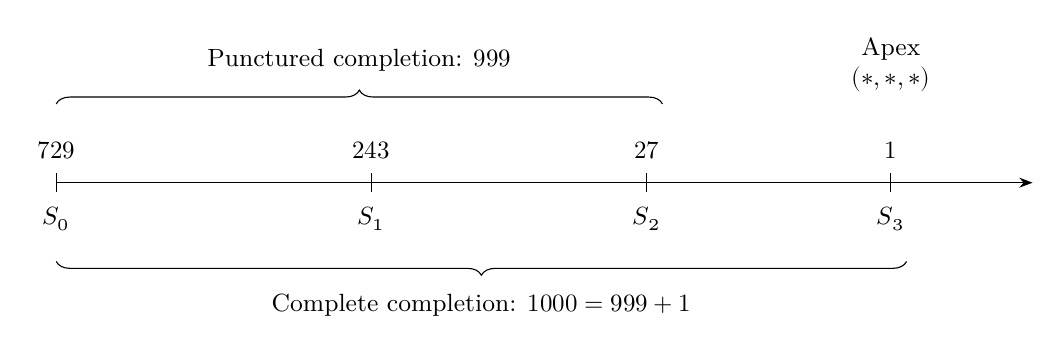
\begin{tikzpicture}[x=1cm,y=1cm,>=Stealth,font=\small]
\draw[->] (0,0)--(12.4,0);
\foreach \x/\a/\b in {0/729/{S_0},4.0/243/{S_1},7.5/27/{S_2},10.6/1/{S_3}}{
  \draw (\x,0.12)--(\x,-0.12);
  \node[above=5pt] at (\x,0) {\(\a\)};
  \node[below=5pt] at (\x,0) {\(\b\)};
}
\draw[decorate,decoration={brace,amplitude=5pt}] (0,1)--(7.7,1);
\node[above=8pt] at (3.85,1) {Punctured completion: \(999\)};
\draw[decorate,decoration={brace,mirror,amplitude=5pt}] (0,-1)--(10.8,-1);
\node[below=8pt] at (5.4,-1) {Complete completion: \(1000=999+1\)};
\node[align=center] at (10.6,1.5) {Apex\\\((\ast,\ast,\ast)\)};
\end{tikzpicture}
\caption{Strata of the cubic completion. The arrangement represents
the set-theoretic decomposition, not a metric scale. The \(243\) elements
of \(S_1\) are three coordinate strata of \(81\) elements; the \(27\)
elements of \(S_2\) are three strata of \(9\). The apex completes the partition.}
\label{fig:revision-emrh}
\end{figure}

% Geometric adaptation of the preserved cubic-completion figure.
\begin{figure}[htbp]
\centering
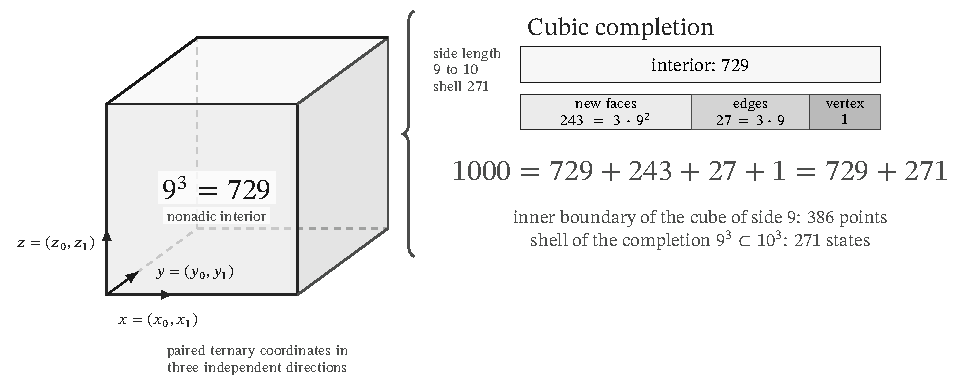
\includegraphics[width=\linewidth]{figures/cubo_emrh.pdf}
\caption{Cubic representation of the expansion from nine to ten classes per coordinate. Strata \(S_1,S_2,S_3\) locate the added incidences on faces, edges, and the apex; their cardinalities form the \(271\)-element shell. The \(386\)-element boundary belongs to the initial cube. This geometric perspective complements the partition in Figure~\ref{fig:revision-emrh}; graphical spacing is schematic.}
\label{fig:completacion-cubo-recuperado}
\end{figure}


\subsubsection{Preservation of unity and dimensional compatibility}

Normalization is not limited to dividing an isolated identity. In dimension
\(d\), the product \(\widehat E^d\) carries the uniform measure
\(\mu_d(\{x\})=10^{-d}\). The coordinate projection
\(p_d:\widehat E^{d+1}\to\widehat E^d\) deletes the final coordinate.

\begin{proposition}[Projective compatibility of the normalized measures]
For every \(d\geq1\),
\[
 (p_d)_*\mu_{d+1}=\mu_d,
 \qquad \mu_d(\widehat E^d)=1.
\]
The mass of the stratum with \(r\) additional coordinates is
\(\binom dr9^{d-r}/10^d\), and the sum of the masses of all strata
is one.
\end{proposition}
\begin{proof}
Every point of \(\widehat E^d\) has ten preimages. Their total mass is
\(10\,10^{-(d+1)}=10^{-d}\). Equality for any subset
is obtained by summing over its points. The stratified formula follows
from the same count as \eqref{eq:revision-estratos}; the binomial
\((9+1)^d\) gives the total normalization.
\end{proof}

In dimension three, removing the apex leaves mass \(999/1000\), and
restoring it adds \(1/1000\). Renormalizing before restoration
would define a different measure: the distinction is operationally relevant.
In particular, preservation of probability mass, preservation of
transport records, and thermodynamic dissipation are assertions concerning
different objects. The proposition proves the first and provides the
compatible support for studying the second; the third requires a
specified dynamical and energetic realization.

The internal geometric boundary likewise remains distinct.
On the Cartesian representative \(\{1,\ldots,9\}^3\), removing
\(\{2,\ldots,8\}^3\) leaves \(386\) points. This boundary belongs to the
initial cube, whereas \(\widehat C\setminus C\) belongs to its
enlargement. The cubic completion, the base-one-thousand positional expansion,
and the exceptional-incidence reading share support data;
their respective maps determine which information from those data is used by
each representation.


\subsection{Cubic incidence and Lorentzian realization}

The cubic completion provides a relation between interior and boundary.
Its geometry can be developed through the incidence of the six faces
with the eight vertices. Label the faces by \((i,\varepsilon)\),
\(i\in\{1,2,3\}\), \(\varepsilon\in\{+1,-1\}\), and the vertices by
\(\nu\in\{+1,-1\}^3\). The incidence matrix is
\[
 M_{(i,\varepsilon),\nu}=\mathbf1_{\{\nu_i=\varepsilon\}}.
\]
Let \(u=(1,\ldots,1)^{\mathsf T}\in\RR^6\), let \(R_F\) denote face
opposition, and let \(P_u=uu^{\mathsf T}/6\), \(P_-=(I-R_F)/2\).

\begin{proposition}[Four-dimensional incidence quotient]
The incidence Gram matrix satisfies
\[
 MM^{\mathsf T}=12P_u+4P_-.
\]
Its eigenvalues \(12,4,0\) have multiplicities \(1,3,2\).
Consequently,
\[
 Q_\square=\RR^6/\ker(MM^{\mathsf T})
 \simeq\RR u\oplus E_-,\qquad E_-=\operatorname{im}P_-.
\]
\end{proposition}
\begin{proof}
A face contains four vertices; two opposite faces have empty intersection,
and two distinct nonopposite faces share two vertices.
The matrix \(12P_u+4P_-\) has precisely those entries.
The uniform space has dimension one; the differences between opposite
faces generate a three-dimensional space orthogonal to the uniform one.
Its complement has dimension two and lies in the kernel.
\end{proof}

The \(1+3\) decomposition arises from incidence. The temporal choice
is specified by the bilinear form
\[
 B_\square([x],[y])=\langle x,(P_--P_u)y\rangle.
\]
It is well defined on the quotient because both projections annihilate the
kernel. In the basis
\[
 t=[u]/\sqrt6,\qquad
 d_i=[e_{i,+}-e_{i,-}]/\sqrt2,
\]
its matrix is \(\operatorname{diag}(-1,1,1,1)\). This makes explicit
the domain, the decomposition, and the sign convention that produce
the Minkowski realization. The positive Gram matrix determines the quotient;
the temporal assignment determines the indefinite form on it.

The operator
\[
 W_\square=\sqrt6P_u+\sqrt2P_-,\qquad
 W_\square e_{i,\varepsilon}=t+\varepsilon d_i
\]
maps the six face labels to null directions, since
\(B_\square(t+\varepsilon d_i,t+\varepsilon d_i)=-1+1=0\).
Direction reversal and face opposition thus acquire a concrete
geometric realization.

\subsubsection{Gluing, reversal, and subdivision}

The cellular realization uses an invertible transport \(U_m(a)\),
which preserves the Lorentzian form, between the fibers at the endpoints of
an oriented dual edge \(a\), a face label
\(\lambda_m(a)\), and an orientation \(\sigma_m(a)\).
With \(\ell_m=\ell_0/9^m\), the gluing map is
\[
 \beta_m(a)=\ell_m\sigma_m(a)
 W_{\square,s(a)}e_{\lambda_m(a)}.
\]
Compatible reversal satisfies
\[
 \beta_m(\bar a)=-U_m(a)\beta_m(a).
\]
Identify the source fibers at two consecutive levels by means of
the specified refinement isometry. If the nine subsegments
\(a_1,\ldots,a_9\), at level \(m+1\), preserve the label
and orientation when transported to that common fiber, then
\begin{equation}
 \beta_m(a)=\sum_{j=1}^9
 U_{m+1}(a_1\cdots a_{j-1})^{-1}\beta_{m+1}(a_j).
 \label{eq:soldadura-refinamiento}
\end{equation}
Each transported term equals \(\ell_m/9\) times the same
null direction, which proves the identity. The compatibility hypothesis
determines which subdivisions realize this refinement.
The equation brings together direction, scale, and transport, instead of reducing
the geometric correspondence to a dimension count.

Once the orientation and Lorentzian form have also been fixed, Hodge duality
on \(\Lambda^2Q_\square^*\) satisfies \(\star^2=-I\).
In dimension four, the sign is \((-1)^{2(4-2)+1}=-1\).
This yields a real complex structure on two-forms and, after
complexification, the eigenspaces with eigenvalues \(+i\) and
\(-i\). The electromagnetic realization will use this domain
after constructing the electronic section and specifying its coupling.

\subsection{Compatibility between modular and positional reductions}

The block-decimal base enters through Euclidean division,
which simultaneously preserves residue and quotient:
\[
 n=1000q+r,\qquad 0\le r<1000.
\]
Since \(1000\equiv1\pmod9\) and \(1000\equiv1\pmod3\),
\[
 n\equiv q+r\pmod9,\qquad n\equiv q+r\pmod3.
\]
Therefore, reduction of a block requires the contribution of the
quotient in order to recover the class of the integer. The numbers \(0\) and
\(1000\) have the same remainder modulo \(1000\), but different classes
modulo \(9\) and modulo \(3\). This is an operational reason to preserve
memory during a change of resolution.

Ternary refinement and determination of a decimal prefix
can be coordinated by means of a single integer residue. If \(N/3^L\)
is a cylinder endpoint and \(D/1000^r\) a decimal endpoint, define
\[
 A=1000^rN-D3^L.
\]
Upon adding six ternary symbols, \(N'=729N+\nu\),
\(L'=L+6\), with \(0\le\nu<729\). If the decimal prefix remains
fixed, then
\[
 A'=729A+\nu1000^r.
\]
If a decimal block \(\delta\) is also incorporated, then
\(D'=1000D+\delta\), \(r'=r+1\), and
\begin{equation}
 A'=729000A+\nu1000^{r+1}-729\delta3^L.
 \label{eq:residuo-dos-bases}
\end{equation}
Both identities are proved by substituting the definitions. Comparison
of endpoints is thus reduced to integer operations that retain the
contribution of each extension. This compatibility is what permits a region
to be refined before its real coordinate is evaluated.

% Incorporated at the end of extension.tex; contains no main section.
% Provenance: RECOVERED_RESULT; sectorial explication of the hypotheses.
% Sources consulted: Holographic Double Projection monograph (editorial source),
% manuscrito/local/01_tesis_recuperada.tex and
% manuscrito/generated/algebra_holonomica.tex, especially §§1--7 and 21.
% Governing definition of number: manuscrito/flattened/main_autosuficiente.tex,
% sections beginning at lines 22137 and 23000 of the 775-page source.
% Its global presentation is not adopted as proof of all TPK arrows.

\subsection{Number as a compatible section and value as a reading}
\label{hist:seccion}

The distinction between state and observation makes it possible to specify which object is
extended as resolution increases. At depth \(n\), let \(X_n\)
be the set of admissible states produced by APP--TRIT--TPK. Their data
include position, sum and product sheets, residues and quotients, regime,
orientation, carry, phase, route, boundary, memory, and survival. These are not
independent coordinates: the arithmetic evaluations and preceding transports
impose their relations. An extension preserves those relations in every
antecedent, even as it adds new steps and new memory data.
This is the meaning of the arithmetic of histories developed self-sufficiently
in this article.

Let \(r_{m,n}:X_m\to X_n\), for \(m\geq n\), be the depth
restrictions, with \(r_{n,n}=\operatorname{id}\) and
\(r_{\ell,n}=r_{m,n}\circ r_{\ell,m}\). Each restriction preserves the
prefix and the information already determined in it.

\begin{definition}[Compatible numerical section]
An HMT number is a compatible history of the system of states:
\begin{equation}
 x=(x_n)_{n\geq0}\in X_\infty:=\varprojlim_n X_n,
 \qquad r_{m,n}(x_m)=x_n.
 \label{hist:limite-inverso}
\end{equation}
A reader is an additional operation on a specified domain of these
histories. A digit is a finite observation; a scalar value is an
evaluation of the reader. The pair formed by the section and its reader constitutes
a read presentation, not a redefinition of the identity of the section.
\end{definition}

On the Archimedean domain \(X_\infty^{\mathrm{Arch}}\), the reader associates
with each prefix a closed cylinder, preserves their nesting, and makes
their diameter tend to zero. It thereby determines
\begin{equation}
 \operatorname{ev}_{\mathbb R}:X_\infty^{\mathrm{Arch}}\longrightarrow
 \mathbb R,\qquad
 \{\operatorname{ev}_{\mathbb R}(x)\}=\bigcap_n I_n(x).
 \label{hist:evaluacion}
\end{equation}
The concrete construction of these cylinders and the determination of their boundaries
are developed in Section~\ref{sec:generacion}. Definition
\eqref{hist:limite-inverso} does not by itself assert that the image of
\eqref{hist:evaluacion} is the entire real line: a coverage assertion
requires its own theorem. Nor does equality of values establish equality of
their histories without an injectivity result. This separation
makes it possible to speak of precision as depth while preserving the distinction
between the arithmetic antecedent and its scalar realization.

\subsection{Composition of histories and memory multiplier}
\label{hist:algebra}

Fix a sector of states at depth \(n\) and a category
\(\mathcal C\) whose arrows are its admissible histories. Composition
is written \(vu=v\circ u\): first \(u\) is traversed and then \(v\).
The elementary steps arise from selection, transport, and the
TPK update. A local tritic fiber can be written
\(\mathbb R[J_x]/(J_x^2+\tau(x)1_x)\), where
\(\tau(x)\in\{+1,0,-1\}\). The regime and orientation belong to the
state being transported; a transition between regimes is not equivalent to
identifying their quadratic algebras.

The following formulation specifies an algebraic sector of that composition.
For each object \(x\), let \(A_x\) be a unital associative real algebra,
which may be noncommutative. For each \(u:x\to y\), let
\(\rho_u:A_x\to A_y\) be a unital homomorphism. Assume a strict action:
\begin{equation}
 \rho_{\operatorname{id}_x}=\operatorname{id}_{A_x},\qquad
 \rho_v\rho_u=\rho_{vu}.
 \label{hist:accion-estricta}
\end{equation}
For each composable pair \(u:x\to y\), \(v:y\to z\), fix an
invertible central multiplier
\(\Omega(v,u)\in Z(A_z)^\times\). Require the normalization
\(\Omega(\operatorname{id}_y,u)=\Omega(u,\operatorname{id}_x)=1_y\)
and, for every composable triple, the identity
\begin{equation}
 \rho_w\bigl(\Omega(v,u)\bigr)\Omega(w,vu)
   =\Omega(w,v)\Omega(wv,u).
 \label{hist:cociclo}
\end{equation}
These are explicit hypotheses on the transports and their coefficients, not a
consequence of calling the dynamics holonomic. When applying this presentation
to a TPK sector, its \(\rho_u\) and \(\Omega(v,u)\) must be identified.
Transitions expressed through bimodules require preservation of that
structure and are not replaced by \eqref{hist:accion-estricta}.

The space of finite sums
\[
 \mathcal H(\mathcal C,A,\rho,\Omega)
   =\bigoplus_{u\in\operatorname{Mor}(\mathcal C)} A_{t(u)}T_u
\]
receives the bilinear product
\begin{equation}
 (aT_v)(bT_u)=a\rho_v(b)\Omega(v,u)T_{vu},
 \label{hist:producto}
\end{equation}
if the arrows are composable, and zero otherwise. Here \(t(u)\)
denotes the terminal state. The sum gathers histories with coefficients; the
product concatenates histories while preserving the record multiplier.

\begin{proposition}[Sectorial associativity with a central multiplier]
Under \eqref{hist:accion-estricta} and \eqref{hist:cociclo}, the product
\eqref{hist:producto} is associative. If the set of objects is finite,
its identity is \(\sum_x1_xT_{\operatorname{id}_x}\).
\end{proposition}
\begin{proof}
For \(u:x\to y\), \(v:y\to z\), \(w:z\to t\), let
\(a\in A_y\), \(b\in A_z\), \(c\in A_t\). The two coefficients
of \(T_{wvu}\) are
\begin{align*}
 ((cT_w)(bT_v))(aT_u):\quad&
 c\rho_w(b)\Omega(w,v)\rho_{wv}(a)\Omega(wv,u),\\
 (cT_w)((bT_v)(aT_u)):\quad&
 c\rho_w(b)\rho_w\rho_v(a)\rho_w(\Omega(v,u))\Omega(w,vu).
\end{align*}
The strict action identifies \(\rho_w\rho_v(a)\) with \(\rho_{wv}(a)\).
Centrality of \(\Omega(w,v)\) permits moving it to the right of
that factor; \eqref{hist:cociclo} then equates the remaining products.
The coefficients \(a,b,c\) are not permuted. If the triple is not composable,
both parenthesizations are zero because of their initial and terminal states.
Bilinearity completes the proof. The local identities and the
normalization of \(\Omega\) verify the stated identity element.
\end{proof}

The calendar carry provides an effective example. In the category
with one object and arrows \(C_9\), take coefficients
\(A=\mathbb R[z,z^{-1}]\), the identity action, and
\[
 \Omega(b,a)=z^{c_0(a,b)},\qquad
 c_0(a,b)=\left\lfloor\frac{a+b}{9}\right\rfloor,
 \quad 0\leq a,b<9.
\]
The two sums of carries of a triple are
\(\lfloor(a+b+c)/9\rfloor\); hence
\eqref{hist:cociclo} holds. The formal variable \(z\) records the circuit without
assigning it a numerical value. Subsequently imposing \(z^{12}=1\) recovers the
dodecaphase register of calendar \eqref{eq:extension108}; retaining
\(z\) without that relation distinguishes successive circuits. The example realizes
the memory of this calendar without identifying it with the entirety of
TPK memory.

\subsection{Dual variance of refinement and preservation of unity}
\label{hist:doble-varianza}

When states are restricted, observables are extended in the opposite direction.
Consider the function algebras, with pointwise product,
\(D_n=\operatorname{Fun}(X_n,\mathbb R)\). Precomposition defines
\begin{equation}
 r_{m,n}^*:D_n\longrightarrow D_m,
 \qquad r_{m,n}^*f=f\circ r_{m,n}.
 \label{hist:precomposicion}
\end{equation}
These are unital morphisms; they are also injective when the corresponding
restrictions are surjective. The direct limit
\(D_{\mathrm{cyl}}=\varinjlim_n(D_n,r_{n+1,n}^*)\) gathers the
finite-depth observations. This algebra is not identified here
with the entire path algebra: extending the transport operators also requires
their compatibilities with refinement.

\begin{lemma}[Unity and naturality of evaluation]
If \(e_x\) is the indicator of \(x\in X_n\), then
\begin{equation}
 r_{m,n}^*e_x=\sum_{y:\,r_{m,n}(y)=x}e_y,
 \qquad r_{m,n}^*1_n=1_m,
 \label{hist:unidad}
\end{equation}
and, for every \(f\in D_n\), \(y\in X_m\),
\[
 \langle r_{m,n}^*f,y\rangle=\langle f,r_{m,n}y\rangle.
\]
Each section \(x\in X_\infty\) determines a well-defined evaluation
\(D_{\mathrm{cyl}}\to\mathbb R\), given by \([f]\mapsto f(x_n)\)
for \(f\in D_n\).
\end{lemma}
\begin{proof}
The fibers of \(r_{m,n}\) form a partition of \(X_m\). Their
indicators are orthogonal and sum to \(1_m\), which proves
\eqref{hist:unidad}. Naturality is the definition of precomposition.
Finally, \((r_{m,n}^*f)(x_m)=f(x_n)\), so two compatible
representatives give the same evaluation in the direct limit.
\end{proof}

The global identity is the constant-one function on all possibilities;
the individual section selects a compatible history. Preserving the
former does not mean immobilizing the latter. Refinement can increase
the number of extensions and the depth of each history while preserving
the identity and all evaluations of its antecedents.

\subsection{Phase return, Weyl representation, and two readings}
\label{hist:puente-lecturas}

Law \eqref{eq:holonomia-memoria} acquires an operator realization
in the bilateral suspension to be constructed in
Section~\ref{sec:generacion}. There \(T\) advances one step,
\(V_9\) observes the nonadic phase, \(W_\delta\) the rotational phase, and
\(D_M\) the memory degree. Writing
\(\widehat\Gamma_9=T^9\) for one circuit in this representation,
the Weyl relations \eqref{eq:weyl-relojes} imply, on vectors
of finite support,
\begin{equation}
 \begin{aligned}
 V_9\widehat\Gamma_9&=\widehat\Gamma_9V_9,\qquad
 W_\delta\widehat\Gamma_9=e^{2\pi i9\delta}
     \widehat\Gamma_9W_\delta,\\
 [D_M,\widehat\Gamma_9]&=\widehat\Gamma_9.
 \end{aligned}
 \label{hist:tres-retornos}
\end{equation}
The first equality follows from \(\zeta_9^9=1\); the second from nine
applications of the covariance of \(W_\delta\); the third expresses
the unit increment of memory. The finite phase returns, while the
irrational rotation and memory distinguish the succeeding state. The
characters and parameter \(\delta\) are realized subsequently from the
numerical construction specified there: they do not retrospectively select
the seeds. This representation describes observables and translations of
the suspension; it does not replace all coordinates or all TPK operators.

The dual reading extends the same distinction between history and observable.
On its Archimedean domain, \eqref{hist:evaluacion} applies; on the
enriched incidence domain, the maps \(Q_n\) of
Section~\ref{exc:doble-lectura} preserve the words and boundary
frames. The equality proved there,
\(r_{n,m}Q_n=Q_mp_{n,m}\), determines its extension \(Q_\infty\).
On the common domain of both readings,
\(\operatorname{ev}_{\mathbb R}(x)\) and \(Q_\infty(x)\) may be considered jointly: the
first retains the value; the second, the transported incidence preserved by its
codomain. The section precedes both. This articulation makes it possible
to pass from the arithmetic of histories to constants and the exceptional
reading without turning their realizations into new initial data.


\clearpage
\section{Joint construction of the continuum through compatible histories and prolongations}
\label{iv:continuo-conjunto}
The arithmetic expressed by a normal form preserves a precise reading of the state that produces it. To situate that reading within HMT, it is also necessary to retain the histories, the sheets, and the operations acting upon them. This chapter brings together that common substrate. Its different constructions are obtained from the same tree of APP–TRIT–TPK executions; the expository divisions allow their properties to be studied without turning them into independent domains chosen by a subsequent application.

The starting point is the formal kernel presented above. An admissible emission contains the APP operation, the TRIT orientation, the change of sheet, the residue and the quotient, together with the effective TPK memory update. When only a residue is expressed, the execution history still belongs to the source object. Two executions with an identical final reading are not identified for that reason alone.

% BEGIN REV09_SUPERVIVENCIA_PUNTO_FIJO
\subsection{Survival by pruning prolongations}
\label{corpus9:xi:supervivencia}

Retrospective memory distinguishes histories recorded by the
APP--TRIT--TPK operations; prospective compatibility organizes their
admissible prolongations. Let \(S\) be the space of complete states
reachable through these operations. Each state retains sheets, residues,
quotients, orientation, carry, memory, and boundary data; whenever a
transition depends on depth, depth forms part of the state.
Let \(E\subseteq S\times S\) be the effective prolongation relation and
\(A\subseteq S\) the admissible set determined by the compatibility of
these records. Admissibility is thus decided through the operations and
boundary conditions that generate the history.

For \(X\subseteq S\), define
\begin{equation}
 \operatorname{Pre}_{E}(X)
 =\{s\in S:\exists t\in X,\ (s,t)\in E\},
 \qquad
 F_{\mathrm{surv}}(X)=A\cap\operatorname{Pre}_{E}(X).
 \label{corpus9:xi:operador-poda}
\end{equation}
The pruning sequence is given by
\begin{equation}
 V_0=A,\qquad
 V_{n+1}=F_{\mathrm{surv}}(V_n),\qquad
 V_\infty=\bigcap_{n\geq0}V_n.
 \label{corpus9:xi:sucesion-poda}
\end{equation}

\begin{proposition}[Survival and the greatest fixed point]
\label{corpus9:xi:mayor-punto-fijo}
The set \(V_n\) consists exactly of the states in \(A\) admitting an
\(n\)-step prolongation all of whose states belong to \(A\). The
sequence \((V_n)\) is decreasing. If each state has finitely many
admissible successors, then
\[
 V_\infty=F_{\mathrm{surv}}(V_\infty)
          =\nu F_{\mathrm{surv}},
\]
where \(\nu F_{\mathrm{surv}}\) denotes the greatest fixed point under
inclusion. Its elements are precisely the states admitting an infinite
compatible prolongation.
\end{proposition}

\begin{proof}
For \(n=0\), a prolongation of length zero consists of the state
itself in \(A\). If the characterization holds for \(n\), a state
belongs to \(V_{n+1}\) exactly when it belongs to \(A\) and has a
successor in \(V_n\); prefixing that edge produces an admissible
prolongation of \(n+1\) steps. This equivalence proves the assertion by
induction. Moreover, \(V_1\subseteq V_0\), and monotonicity of
\(F_{\mathrm{surv}}\) propagates \(V_{n+1}\subseteq V_n\).

Let \(s\in V_\infty\), and write
\(E(s)=\{t\in S:(s,t)\in E\}\). Since \(s\in V_{n+1}\) for every \(n\),
the sets \(E(s)\cap V_n\) are nonempty, finite, and decreasing.
Their intersection contains an element \(t\), which belongs to
\(V_\infty\) and satisfies \((s,t)\in E\). Hence
\(V_\infty\subseteq F_{\mathrm{surv}}(V_\infty)\).
Conversely, monotonicity gives
\(F_{\mathrm{surv}}(V_\infty)\subseteq V_{n+1}\) for every \(n\);
the image also lies in \(A=V_0\), and therefore belongs to
\(V_\infty\). This proves the fixed-point equality.

If \(W=F_{\mathrm{surv}}(W)\), then \(W\subseteq A=V_0\).
From \(W\subseteq V_n\) it follows that
\(W=F_{\mathrm{surv}}(W)\subseteq F_{\mathrm{surv}}(V_n)=V_{n+1}\).
Induction yields \(W\subseteq V_\infty\), proving maximality.
Finally, the prolongation tree of a state in \(V_\infty\) is finitely
branching and has a nonempty level at every depth. K\"onig's lemma
provides an infinite branch. Conversely, the prefixes of any infinite
prolongation place its initial state in every \(V_n\).
\end{proof}

\paragraph{Branching and stabilization.}
The finiteness hypothesis has an explicit control. Consider a root
with a distinct terminal branch of each positive integer length, all
branches being admissible and disjoint after the root. The root
admits prolongations of every finite length and belongs to all the
\(V_n\); each of its successors belongs to a branch of bounded length.
Consequently, the root has neither an infinite prolongation nor a
successor in \(V_\infty\). This tree has infinite branching at the
root. In contrast, if \(A\) is finite, each strict inclusion
\(V_{n+1}\subsetneq V_n\) removes at least one state. Pruning reaches
a fixed point after at most \(|A|\) strict layer removals.
This bound pertains to the finite domain \(A\).

\paragraph{Uniqueness of continuation.}
For \(s\in V_\infty\), the successors retaining survival form
\[
 E(s)\cap V_\infty.
\]
The next state is uniquely selected exactly when
\begin{equation}
 \#\bigl(E(s)\cap V_\infty\bigr)=1.
 \label{corpus9:xi:unicidad-sucesor}
\end{equation}
An infinite prolongation is unique when this condition holds at
each state of the path. Indeed, each surviving successor has an
infinite prolongation by the preceding proposition; two distinct
successors produce two distinct paths. When the successor is unique
at each step, the prefixes are determined successively.
Several viable successors express multiplicity of prolongations
within the same survival domain.

\begin{proposition}[Conjugation of the two directions of prolongation]
\label{corpus9:xi:conjugacion-supervivencia}
Let \(C:S\to S\) be an involution such that \(C(A)=A\) and
\begin{equation}
 (x,y)\in E\quad\Longleftrightarrow\quad(Cy,Cx)\in E.
 \label{corpus9:xi:involucion-prolongaciones}
\end{equation}
Let \(V_n^+\) denote pruning for \(E\), and \(V_n^-\) pruning for
\(E^{-1}\), both with initial set \(A\). Then
\[
 C(V_n^+)=V_n^-\quad(n\geq0),\qquad
 C(V_\infty^+)=V_\infty^-.
\]
\end{proposition}

\begin{proof}
If \(s_0,\ldots,s_n\) is an admissible path for \(E\), the sequence
\(Cs_0,\ldots,Cs_n\) is an admissible path for \(E^{-1}\):
for each \(j\), the hypothesis converts
\((s_j,s_{j+1})\in E\) into \((Cs_{j+1},Cs_j)\in E\).
All its states belong to \(A\). Applying the same operation again
recovers the initial path because \(C^2=I\); it therefore establishes
a bijection between finite prolongations in the two directions.
The characterization of \(V_n^\pm\) by paths gives
\(C(V_n^+)=V_n^-\). Since \(C\) is bijective, it commutes with the
intersection of these sets, yielding the equality for
\(V_\infty^\pm\).
\end{proof}

The involution transports the surviving set in one direction to
the surviving set in the conjugate direction. Infinite
prolongability in both directions corresponds to
\(V_\infty^+\cap V_\infty^-\); uniqueness of a path retains the
criterion in \eqref{corpus9:xi:unicidad-sucesor}. Retaining a
genealogy and restricting its continuation tree are two typed
operations on the same records. Assigning an entropy to these
readings additionally requires the corresponding measure on histories.
% END REV09_SUPERVIVENCIA_PUNTO_FIJO


\subsection{Admissible histories and memory by composition}
Let \(H_0:=\{\ast\}\). The level \(H_1\) is the finite nonempty set of
admissible APP--TRIT seeds, and, for \(k\geq1\), \(H_k\) is the set of
enriched histories of length \(k\) admitting compatible TPK prolongations
at every finite horizon. Its elements are constructed through successive emissions
from the initial domain of the kernel. We write \(\zeta\varepsilon\)
for the prolongation of \(\zeta\) by an admissible emission \(\varepsilon\), and
\(\rho_k(\zeta\varepsilon)=\zeta\) for deletion of the final emission. The label
produced by the emission is retained, even when different labels express
the same scalar state. The space of complete histories is defined by
\[
 H_\infty^{\rm enr}:=\varprojlim_k(H_k,\rho_k).
\]
The cofinal subsystem \(X_N:=H_{6N}\), with \(X_0=H_0\), coincides with the
sextet clock used in the cardinal proof; by cofinality there is a canonical
identification
\(H_\infty^{\rm enr}\cong\varprojlim_N(X_N,\rho_{6(N+1),6N})\).

On the two arithmetic sheets, the local data satisfy the exact divisions

\[
\delta_\diamond=r_\diamond+9q_\diamond,
\qquad 0\leq r_\diamond<9,
\qquad \diamond\in\{\Sigma,\Pi\}.
\]
The oriented TRIT coordinate similarly admits an expression \(\Delta=o_r+3\kappa\), with the oriented representative declared by the kernel. Preservation of the quotient allows these representations to be composed without replacing an emission by its isolated residue.

In a memory chart, the update of an emission is written

\[
U_\varepsilon(m)=C_\varepsilon m+\kappa_\varepsilon.
\]
For a path \(\alpha=(\varepsilon_1,\ldots,\varepsilon_k)\), the effective operation is the ordered composition of those updates. Its linear part and its translation are

\[
C_\alpha=C_{\varepsilon_k}\cdots C_{\varepsilon_1},
\qquad
\kappa_\alpha=
\sum_{j=1}^{k}C_{\varepsilon_k}\cdots
C_{\varepsilon_{j+1}}\kappa_{\varepsilon_j}.
\]
The empty product in the last sum is the identity.

\begin{proposition}[Affine compatibility of concatenation]
\label{prop:continuo-compatibilidad-afin}
If \(\alpha\) precedes \(\beta\), then

\[
C_{\beta\alpha}=C_\beta C_\alpha,
\qquad
\kappa_{\beta\alpha}=C_\beta\kappa_\alpha+\kappa_\beta,
\qquad
U_{\beta\alpha}=U_\beta U_\alpha.
\]
\end{proposition}
\begin{proof}
Substituting \(U_\alpha(m)\) into \(U_\beta\) yields \(C_\beta C_\alpha m+C_\beta\kappa_\alpha+\kappa_\beta\). Decomposition into linear part and translation gives the three identities. Associativity of composition proves that the result does not depend on an auxiliary subdivision of the path.
\end{proof}

This cocycle identity is the precise content of the accumulated memory. The quantity transported by a second path depends on the chart update it performs; in general, it is not the untransported sum of two records.

The nonadic return preserves a second distinction. In the phase and turn coordinates, with \(\bar r\in\{0,\ldots,8\}\), its representation is

\[
\sigma_9(w,r)=
\left(w+\left\lfloor\frac{\bar r+1}{9}\right\rfloor,
r+1\pmod9\right),
\qquad
\sigma_9^9(w,r)=(w+1,r).
\]
Over nine steps, exactly one crossing from \(8\) to \(0\) occurs. The phase returns and the turn coordinate increases. The enriched holonomy also retains the memory updates accompanying that traversal.

\subsection{Tree refinement and measure of histories}
The initial measure is the canonical one from the census: \(\mu(\ast)=1\) and
\(\mu(c)=1/|H_1|\) for each seed \(c\in H_1\). In this subsection, each
history has a finite positive number of prolongations. Deletion of
emissions defines the refinement maps. Admissibility of the kernel
provides the prolongations; when a residence uses a neutral emission,
that emission explicitly provides a section of \(\rho_k\). The existence of this
section concerns the tree that includes that emission, not an arbitrary
restriction of routes.

Let \(d(\zeta)\geq1\) be the number of admissible emissions at \(\zeta\). The
APP order and the census of prolongations determine the canonical law
\(p_{\rm can}(\varepsilon\mid\zeta)=1/d(\zeta)\). Without additional
parameters, this law defines

\[
\mu(\zeta\varepsilon)=\frac{\mu(\zeta)}{d(\zeta)}.
\]
A nonuniform weighting may replace \(p_{\rm can}\) only when it has already
been produced and added to the enriched record. The correlative constructor
of this chapter uses \(p_{\rm can}\) exclusively; therefore, its measure
is a function of the APP--TRIT--TPK tree and not of an external choice.

\begin{proposition}[Cylindrical compatibility and conditional expectation]
\label{prop:continuo-esperanza-condicional}
At every level,

\[
\sum_{\rho_k(y)=x}\mu(y)=\mu(x).
\]
In the spaces \(L^2(H_k,\mu_k)\), the maps

\[
(\mathsf J_kf)(y)=f(\rho_k(y)),
\qquad
(E_kg)(x)=\sum_{\rho_k(y)=x}\frac{\mu(y)}{\mu(x)}g(y)
\]
satisfy \(E_k=\mathsf J_k^*\), \(E_k\mathsf J_k=I\), and \(\|\mathsf J_kf\|=\|f\|\).
\end{proposition}
\begin{proof}
The first identity is the normalization of the local probabilities. Applying it to \(|f(x)|^2\) yields the isometry. Grouping the sum by fibers of \(\rho_k\) yields the formula for \(E_k\); on a function constant on each fiber, that formula returns its value.
\end{proof}

The compatible masses define a probability measure on the space of infinite histories: the cylinder of a finite history receives its mass \(\mu(\zeta)\). The measure extends from the algebra of cylinders, and its uniqueness follows because they generate the \(\sigma\)-algebra. If the tree is finitely branching and every history has a prolongation, the inverse limit of its levels under deletion of emissions is nonempty. In the cylinder topology, every nonempty cylinder has positive measure.

This measure distinguishes histories converging to the same representation. The uniform measure on terminal values would be a different reading, since it would eliminate the multiplicities that the construction has just preserved.

\subsubsection{Enriched readers and fiber memory}
\label{sec:ch-memoria-fibra}

The difference between history and value admits an operational criterion. At a
finite level \(H_k\), let \(q_k:H_k\to Z_k\) be a reader and let
\(M_k:H_k\to\mathcal M_k\) be the preserved record. The enriched reader
is \(\widehat q_k=(q_k,M_k)\). Memory distinguishes states within a single
fiber of the reader; its sufficiency is verified on the domain under consideration.
This formulation incorporates into the article itself the complete development of the
fiber information used below.

\begin{proposition}[Recoverability at a finite level]
\label{prop:ch-recuperabilidad-fibra}
An inverse of \(\widehat q_k\) exists on its image if and only if
\(\widehat q_k\) is injective. For a random variable \(Z\) taking
values in \(H_k\) with distribution \(\mu_k\),
\[
 \mathsf H(Z)=\mathsf H(q_k(Z))+\mathsf H(Z\mid q_k(Z)).
\]
If \(\widehat q_k\) is injective on the support of \(Z\), then
\[
 \mathsf H(Z\mid q_k(Z),M_k(Z))=0.
\]
Here \(\mathsf H(Z)=-\sum_z\Pr(Z=z)\log\Pr(Z=z)\), with
\(0\log0=0\), is finite entropy in nats; conditional entropy is
the average entropy of the conditional distributions.
\end{proposition}

\begin{proof}
An inverse recovers a unique antecedent, which requires injectivity;
conversely, injectivity makes it possible to assign to each expressed pair its unique
antecedent. Since \(q_k(Z)\) is a deterministic function of \(Z\),
grouping the sum defining \(\mathsf H(Z)\) by fibers of \(q_k\) yields the
chain rule. If the pair \((q_k(Z),M_k(Z))\) distinguishes the support,
each corresponding conditional distribution is concentrated on a single
state, and its entropy is zero.
\end{proof}

Not publishing a coordinate and erasing the record that permits its recovery are
distinct operations. This result does not identify entropy with the cardinality
of the continuum or introduce a thermal interpretation: its domain, reader, and
distribution are precisely those just specified.

\subsubsection{Equivariance of the measure under tree symmetries}
\label{sec:ch-naturalidad-medida}

\begin{proposition}[Joint transport of the tree and its measure]
\label{prop:ch-naturalidad-medida}
Let \(g=(g_k)_{k\geq0}\) be a collection of bijections \(g_k:H_k\to H_k\)
that commutes with truncations, fixes the root, and bijectively transports
admissible emissions while preserving their multiplicities. Then
\[
 d(g_k\zeta)=d(\zeta),\qquad
 (g_k)_*\mu_k=\mu_k,\qquad (g_\infty)_*\mu=\mu.
\]
More generally, if \(\mu_\zeta\) is the law of continuations of a
history \(\zeta\in H_k\), then
\[
 (g_\infty)_*\mu_\zeta=\mu_{g_k\zeta}.
\]
\end{proposition}

\begin{proof}
The bijection of emissions preserves their number with multiplicities. The
uniform seed distribution is likewise invariant. Each path
and its image therefore receive the same product of local weights
\(1/d(\zeta)\). Equality of measures follows at every level and on
every cylinder. Compatibility with truncations defines \(g_\infty\),
and uniqueness of the measure determined by cylinders proves equality
in the limit. The same argument, beginning at \(\zeta\), proves the
assertion about continuations.
\end{proof}

This establishes the naturality of the tree and its measure: a coherent change
of representation transports the weights and does not require choosing them anew.
Preservation of emissions and multiplicities is an essential hypothesis of
the proposition, not a datum added after the construction.


\subsection{Transport by sheets and exact accounting of outputs}
First consider the space with orthonormal basis formed by the histories at level \(k\). The transport preserving the label of each prolongation is

\[
\mathcal U_ke_\zeta=
\sum_{\varepsilon\ \mathrm{admissible\ at}\ \zeta}
\sqrt{p_{\rm can}(\varepsilon\mid\zeta)}\,e_{\zeta\varepsilon}.
\]
The successor fibers of distinct antecedents are disjoint. The normalization of \(p_{\rm can}\) therefore proves \(\mathcal U_k^*\mathcal U_k=I\). The representation by masses of histories is related to this one by the diagonal change of basis incorporating \(\sqrt{\mu(\zeta)}\).

The sheet label is part of the complete record of a history. We write
\[
\widehat\zeta=((\zeta_0,s_0),\ldots,(\zeta_k,s_k)),\qquad
s_j\in\{\Sigma,\Pi\},
\]
where \(s_j\) is the active sheet at step \(j\). The prolongation adds the emission and the sheet \(s_{k+1}\) determined by the operational TPK selector, retaining the prefix in full, including the initial sheet. In the basis of these lifted histories,
\[
\mathcal U_ke_{\widehat\zeta}
=\sum_{\varepsilon\ \mathrm{admissible\ at}\ \widehat\zeta}
\sqrt{p_{\rm can}(\varepsilon\mid\widehat\zeta)}\,e_{\widehat\zeta\varepsilon},
\qquad
P_ke_{\widehat\zeta}=\mathbf1_{s_k=\Sigma}e_{\widehat\zeta},\quad
Q_k=I-P_k.
\]
Thus, \(P_k\) reads the current sheet, while the distinction between histories is maintained by their complete prefixes. Two initial histories that reach the same active sheet retain distinct successor fibers. The proof of isometry by disjoint collections of prolongations applies verbatim to this basis.
The tritic orientation is another coordinate of the record: the value \(0\) preserves the threshold reading on each sheet and does not add a third sheet to this decomposition. We now separate sheet preservation and sheet exchange:

\[
A_k=P_{k+1}\mathcal U_kP_k+Q_{k+1}\mathcal U_kQ_k,
\qquad
\eta_k=Q_{k+1}\mathcal U_kP_k+P_{k+1}\mathcal U_kQ_k.
\]
\begin{proposition}[Gram identity by sheets]
\label{prop:continuo-gram-hojas}
For a linear transport \(U\), whether or not it is isometric, the preceding decomposition satisfies

\[
A^*A+\eta^*\eta=PU^*UP+QU^*UQ.
\]
In particular, for \(U=\mathcal U_k\),

\[
A_k^*A_k+\eta_k^*\eta_k=I.
\]
\end{proposition}
\begin{proof}
In \(A^*A\) and \(\eta^*\eta\), the mixed terms containing \(P_{k+1}Q_{k+1}\) vanish. Summing the remaining terms produces \(P_kU^*(P_{k+1}+Q_{k+1})UP_k\), and its analogue with \(Q_k\). The first identity follows from complementarity of the projectors; the second also uses \(U^*U=I\).
\end{proof}

The first identity is the general formula. Replacing its right-hand side by \(U^*U\) requires the cross-blocks of that Gram matrix to vanish. Isometric preservation of history transport provides that condition here; it must not be attributed automatically to a subsequent compression.

Write \(F_{0,0}=I\), \(F_{0,n}=A_{n-1}\cdots A_0\), and \(T_N=F_{0,N}^*F_{0,N}\).

\begin{theorem}[Finite decomposition with terminal residue]
\label{thm:continuo-descomposicion-terminal}
For each horizon \(N\),

\[
I=\sum_{n=0}^{N-1}
F_{0,n}^*\eta_n^*\eta_nF_{0,n}+T_N.
\]
The sequence \(T_N\) is positive and decreasing, and has a positive strong limit \(T_\infty\). The sum of outputs converges strongly to \(I-T_\infty\).
\end{theorem}
\begin{proof}
Proposition~\ref{prop:continuo-gram-hojas} gives \(T_n-T_{n+1}=F_{0,n}^*\eta_n^*\eta_nF_{0,n}\). The telescoping sum proves the finite equality and monotonicity. For each vector, the quadratic forms decrease to a limit; polarization defines a positive bounded form and, by the representation theorem for bounded forms, an operator \(T_\infty\). Convergence is strong because, for a positive operator \(S\leq I\), \(\|Sv\|^2\leq\langle v,Sv\rangle\); this is applied to \(S=T_N-T_\infty\).
\end{proof}

The terminal residue is retained until its extinction in the domain under consideration is proved. This distinction prevents a phase return, by itself, from becoming an assumption that all histories are exhausted.

\subsection{Oriented balance and cancellation under refinement}
A history carries its accumulated orientation \(o(h)\) and the counts of its visits to the two sheets. The corresponding local balance is

\[
b(h)=o(h)\bigl(N_\Sigma(h)-N_\Pi(h)\bigr),
\qquad
b^+=\frac{|b|+b}{2},\quad b^-=\frac{|b|-b}{2}.
\]
When a reader expresses the mean over the prolongations, \(b_c=Eb_f\) is defined. The orientation remains in the argument of \(b_f\); it is not removed before averaging.

\begin{proposition}[Exact cancellation defect]
\label{prop:continuo-defecto-cancelacion}
The quantity

\[
\kappa_{\mathrm{can}}=
\frac{E|b_f|-|Eb_f|}{2}
\]
is nonnegative and satisfies

\[
E(b_f^+)=(b_c)^++\kappa_{\mathrm{can}},
\qquad
E(b_f^-)=(b_c)^-+\kappa_{\mathrm{can}}.
\]
\end{proposition}
\begin{proof}
The weighted triangle inequality gives \(|Eb_f|\leq E|b_f|\). Writing the positive and negative parts as \((|b|\pm b)/2\) yields both equalities.
\end{proof}

The information omitted when only the balance is expressed is the common cancellation of the opposing contributions. This quantity is determined from the same prolongations used by the preceding transport. The factor \(1/9\) appears only when the fiber contains nine prolongations with equal weights; conditional expectation is the rule that remains valid for general branching and weightings.

\subsection{Ternary incidence of the sheets and rectangular complex}
The two sheets determine the module \(V=\mathbb F_3e_\Sigma\oplus\mathbb F_3e_\Pi\). Its four projective directions are the lines generated by \(e_\Sigma,e_\Pi,e_\Sigma+e_\Pi,e_\Sigma-e_\Pi\). They give rise to six unordered pairs. The eight nonzero vectors are their oriented representatives. Thus, the counts \(4,6,8\) belong to distinct operations on the same sheet module.

On the six pair positions, define

\[
(Ba)_{\{L,L'\}}=a_L+a_{L'},
\qquad
s(q)=\sum_{\{L,L'\}}q_{\{L,L'\}}.
\]
Each direction occurs in three pairs; hence \(sB=0\) in \(\mathbb F_3\). The reader \(W(q)=\mathbf1_{s(q)=0}-1/3\) is invariant under \(q\mapsto q+Ba\). On the uniform ambient space \(\mathbb F_3^6\), its moments are

\[
\mathbb EW=0,\qquad
\mathbb EW^2=\frac29,\qquad
\mathbb EW^3=\frac2{27}.
\]
Indeed, \(s\) is surjective and each fiber contains \(3^5\) elements. The reader equals \(2/3\) with probability \(1/3\) and \(-1/3\) with probability \(2/3\). These means describe the uniform ambient space; the distribution induced by a subset of histories must be calculated with its own multiplicities, already retained in \(H_k\).

To fix the ports without losing multiplicities, at depth \(k\) the
labeled readings are retained:
\(\lambda_\Sigma(\zeta)=(\zeta,\Sigma)\) and
\(\lambda_\Pi(\zeta)=(\zeta,\Pi)\). Their sets are
\[
\mathscr P_k^\Sigma=\{\lambda_\Sigma(\zeta):\zeta\in H_k\},\qquad
\mathscr P_k^\Pi=\{\lambda_\Pi(\zeta):\zeta\in H_k\}.
\]
They are finite and nonempty because \(H_k\) is. Values, quotients, and residues
are expressed on these ports; equality of values does not identify their
labels. The product \(\mathscr P_k^\Sigma\times\mathscr P_k^\Pi\) is the
domain of the rectangular reading, within which the support of the
admissible incidences is recorded.

With this level fixed, write \(I=\mathscr P_k^\Sigma\),
\(J=\mathscr P_k^\Pi\), and \(A_m=\mathbb Z/3^m\mathbb Z\). The
lexicographic APP order determines the minimal surviving branch and, within it, the
reference ports \(i_0,j_0\). No external choice is added: changing
coordinates produces a canonically isomorphic complex. The maps

\[
\kappa(u,v)_{ij}=u_i-v_j,
\qquad
(\delta w)_{ij}=w_{ij}-w_{ij_0}-w_{i_0j}+w_{i_0j_0}
\]
define the following sequence, valid over the finite ring \(A_m\):

\[
0\longrightarrow A_m\longrightarrow
A_m^I\oplus A_m^J\mathrel{\mathop{\longrightarrow}^{\kappa}}
A_m^{I\times J}\mathrel{\mathop{\longrightarrow}^{\delta}}
A_m^{(I\setminus\{i_0\})\times(J\setminus\{j_0\})}
\longrightarrow0.
\]
\begin{proposition}[Exactness of rectangular incidence]
\label{prop:continuo-exactitud-rectangular}
The preceding sequence is exact, with its first arrow given by the constant diagonal.
\end{proposition}
\begin{proof}
The equality \(u_i-v_j=0\) for every pair forces all coordinates of \(u\) and \(v\) to be the same constant. Direct substitution gives \(\delta\kappa=0\). If \(\delta w=0\), take \(u_i=w_{ij_0}\) and \(v_j=w_{i_0j_0}-w_{i_0j}\). Then \(u_i-v_j=w_{ij}\). Finally, any matrix in the last term is prolonged with zero reference row and column; its image under \(\delta\) is the initial matrix. The proof uses only additions and subtractions, and therefore does not require division by a unit of the ring.
\end{proof}

Reduction from \(A_{m+1}\) to \(A_m\), while keeping
\(k,\mathscr P_k^\Sigma,\mathscr P_k^\Pi,i_0,j_0\) fixed, commutes with both
maps. The reconstruction formulas are the same at every modular
depth. This is the arithmetic compatibility proved in this subsection. The
prolongation of histories \(k\to k+1\) preserves the prefix labels; its
maps between sets of ports are data distinct from the change of
ring \(m\to m+1\).

Those maps are obtained from deletion of emissions:
\[
\rho_k^\Sigma(\zeta\varepsilon,\Sigma)=(\zeta,\Sigma),\qquad
\rho_k^\Pi(\zeta\varepsilon,\Pi)=(\zeta,\Pi).
\]
The minimal surviving branch of the APP order just constructed has compatible prolongations. Its two labels define compatible reference ports at every level. Coordinate transport is precomposition:
\[
(L_ku)_{i'}=u_{\rho_k^\Sigma(i')},\quad
(L_kv)_{j'}=v_{\rho_k^\Pi(j')},\quad
(L_kw)_{i'j'}=w_{\rho_k^\Sigma(i'),\rho_k^\Pi(j')}.
\]
For the last module in the sequence, the matrix is first prolonged by zero on the reference row and column, this same formula is applied, and the result is restricted to the new complement of the reference ports. This rule also defines \(L_k\) when a new port has the marked port as its antecedent.

\begin{proposition}[Naturality of the rectangular complex under prolongation]
\label{iv:rectangular-natural}
The preceding maps satisfy
\(L_k\kappa_k=\kappa_{k+1}L_k\) and
\(L_k\delta_k=\delta_{k+1}L_k\).
They also commute with coefficient reduction
\(A_{m+1}\to A_m\) and compose in accordance with prefix deletion.
\end{proposition}
\begin{proof}
The first identity follows from
\(u_{\rho_k^\Sigma(i')}-v_{\rho_k^\Pi(j')}\).
In the second, each of the four terms defining \(\delta\)
is transported by the same precomposition. Compatibility of the
marked ports identifies their rows and columns; when an antecedent is
the marked port, the four terms cancel and agree with
prolongation by zero. All formulas are sums and differences with
integer coefficients, so they commute with modular reduction.
The composition of precompositions is precomposition with the
composite prefix, proving the final assertion.
\end{proof}

\subsection{Memory complex and compatibility of incidences}
The same accumulated memory coordinate \(c_y\in\mathbb Z\), at a residence \(y\), defines a free integral complex. Its reduction to \(A_m\) uses the same integer record before reduction; therefore, successive depths are compatible. Its generators are \(f_y\) in degree \(2\), \(e_y,b_y,r_y\) in degree \(1\), and \(g_y\) in degree \(0\):

\[
\partial f_y=3c_y e_y+b_y,\qquad
\partial e_y=g_y,\qquad
\partial b_y=-3c_y g_y,\qquad
\partial r_y=0.
\]
The identity \(\partial^2=0\) is verified on \(f_y\) by \(3c_yg_y-3c_yg_y=0\), and is immediate on the other generators.

If a path \(\alpha:y\to y'\) updates the memory, its transport in the complex sends the like-named generators to their new representatives, except for

\[
\Psi_\alpha(b_y)=b_{y'}+3(c_{y'}-c_y)e_{y'}.
\]
\begin{proposition}[Naturality of the memory complex]
\label{prop:continuo-naturalidad-memoria}
The identities \(\partial\Psi_\alpha=\Psi_\alpha\partial\) and \(\Psi_{\beta\alpha}=\Psi_\beta\Psi_\alpha\) hold. The maps extend linearly over the chosen coefficient ring.
\end{proposition}
\begin{proof}
On \(f_y\), the image of its boundary is \(3c_ye_{y'}+b_{y'}+3(c_{y'}-c_y)e_{y'} =3c_{y'}e_{y'}+b_{y'}\). On \(b_y\), the boundary of its image is \(-3c_{y'}g_{y'}+3(c_{y'}-c_y)g_{y'}=-3c_yg_{y'}\). The other two cases are immediate. Under concatenation, the memory differences sum telescopically, proving the second identity.
\end{proof}

The relation between two representatives of the same residence can also be written as an explicit boundary. For an integer coordinate \(v\), reduced in the same ring when appropriate, let

\[
z^-=r_y,\qquad z^+=r_y+3c_yv e_y+v b_y,
\qquad h_*=-vf_y.
\]
Then \(\partial h_*=z^--z^+\). Under a transport that also updates \(v\), the correction \(K_\alpha=(v_{y'}-v_y)f_{y'}\) satisfies \(K_{\beta\alpha}=K_\beta+\Psi_\beta K_\alpha\). The symbols \(K_\alpha\) in this local homotopy do not denote the dodecaphase seal \(K\): they belong to another domain, and their function is specified by the preceding identity. Their function can also be checked in the equality

\[
z^+_{y'}-\Psi_\alpha z^+_y=\partial K_\alpha.
\]
Both sides equal \((v_{y'}-v_y)(3c_{y'}e_{y'}+b_{y'})\).

\begin{proposition}[Homology and memory of the local complex]
\label{prop:continuo-homologia-memoria}
Over \(\mathbb Z\), or after reduction to \(A_m\), one has

\[
H_0(\Gamma)=H_2(\Gamma)=0,
\qquad H_1(\Gamma)\cong A_m[r_y]
\]
in the modular realization, and \(H_1(\Gamma)\cong\mathbb Z[r_y]\) in the integral realization.
\end{proposition}
\Needspace{9\baselineskip}
\begin{proof}
Define the degree-\(1\) homotopy by \(h(g_y)=e_y\), \(h(b_y)=f_y\), and zero on the other generators. Let \(p\) be the projection onto the summand generated by \(r_y\), and \(\iota\) its inclusion. Verification on each generator gives

\[
\partial h+h\partial=I-\iota p.
\]
In particular, on \(b_y\) the terms \(3c_ye_y\) and \(-3c_ye_y\) cancel. The complex deformation retracts onto the module generated by \(r_y\), concentrated in degree \(1\), proving the assertion.
\end{proof}

The transport \(\Psi_\alpha\) is a shear of determinant \(1\). Thus, this complex explicitly preserves how \(c_y\) changes at chain level, but its local homology does not distinguish the values of that coordinate. The complete memory remains in the labels and transports of the source state; it is not recovered from \(H_1\) alone. A memory-dependent numerical torsion requires the specified assembly and determinant reading, in addition to this local complex.

\subsection{Assembly with terminal paths}
For a finite horizon, the residences and their prolongations form a path category. Each residence \(\nu\) is assigned the free module \(W(\nu)=A_m[\operatorname{Path}(\nu,\mathrm{Term})]\), which retains each terminal continuation as a generator. An initial path acts on \(W\) by precomposition. The complex \(\Gamma(\nu)\) of the preceding subsection acts covariantly through \(\Psi\).

The assembly uses both transports in the same bigraded module:

\[
\mathcal B_{q,r}=
\bigoplus_{\nu_0\to\cdots\to\nu_q}
W(\nu_q)\otimes_{A_m}\Gamma_r(\nu_0).
\]
The normalized path complex is used: degenerate chains containing identities are omitted. The finite horizon then bounds the number of strict prolongations and the horizontal degree. The horizontal boundary deletes an intermediate residence by composing the adjacent arrows. At the first endpoint it transports \(\Gamma\); at the last it precomposes \(W\). Alternating signs give the path boundary \(d_{\mathrm{bar}}\). The total differential is

\[
D=d_{\mathrm{bar}}+(-1)^q\partial_\Gamma.
\]
The face identities cancel the terms of \(d_{\mathrm{bar}}^2\) pairwise. Naturality in Proposition~\ref{prop:continuo-naturalidad-memoria} implies that \(d_{\mathrm{bar}}\) commutes with \(\partial_\Gamma\); the factor \((-1)^q\) cancels the cross terms in the square. Therefore, \(D^2=0\). Compatibility is proved on path generators and is not introduced by a label asserting membership in a complex.

Terminal evaluation also does not require choosing a particular history. For each continuation \(h\), the effective composition of its updates is applied. The result retains the pair formed by \(h\) and its reading, with its multiplicity. If \(k<\ell<N\), the continuations decompose as a disjoint union of prefixes up to \(\ell\) and their continuations up to \(N\). Proposition~\ref{prop:continuo-compatibilidad-afin} proves that direct evaluation and evaluation of those two parts produce the same reading. This yields the terminal naturality square.

The path modules, incidences, memory transport, and their differentials arise from the same prolongations. Their assembly does not consist in adding to a state five coordinates that would be retained by definition: their relations are constructed through sums, boundaries, and effective compositions, and are verified on their generators.

\subsection{Determinants, limit, and arithmetic reading}
At each residence, the free local complex \(\Gamma\) admits its graded determinant line

\[
\operatorname{Det}\Gamma=
\bigotimes_r\left(\bigwedge^{\mathrm{rk}\Gamma_r}\Gamma_r\right)^{(-1)^r}.
\]
The total assembly of the preceding subsection, in turn, has the modules \(\operatorname{Tot}_d\mathcal B=\bigoplus_{q+r=d}\mathcal B_{q,r}\). At finite horizon and over the same ring, they are free of finite rank and only finitely many of them are nonzero. Its line is
\[
\operatorname{Det}(\operatorname{Tot}\mathcal B)=
\bigotimes_{q,r}
\left(\bigwedge^{\operatorname{rk}\mathcal B_{q,r}}
\mathcal B_{q,r}\right)^{(-1)^{q+r}}.
\]
This formula follows from the direct-sum decomposition in each degree. It distinguishes the line of the local complex from that of the assembly with all paths; their bases are ordered by means of the retained labels. Modular reduction commutes with these exterior powers because the modules and their bases arise from the same free integral modules at fixed horizon.
The line is defined by the modules and their degrees, both over \(\mathbb Z\) and after reduction to \(A_m\); a negative exponent denotes the dual module. A nonzero numerical torsion additionally requires specifying the complex over a field, the bases, and the relevant homology identifications. To calculate Smith factors, one uses the integer matrix produced before reduction, not an arbitrary lift of a modular matrix. An integer square block with nonzero determinant is invertible over \(\mathbb Q\); its reduction is invertible over \(A_m\) only when that determinant is a unit, that is, when it is not divisible by \(3\). Refinement of memories and incidences makes it possible to formulate and verify the stability of the relevant invariant factors; these conditions do not follow from the existence of the determinant line.

Passage to the limit preserves the compatible projective systems of residues, the histories, and their multiplicities. The squares proved in the preceding subsections remain commutative because their maps are given by the same formulas at each level. For an Archimedean coordinate, the additional step consists in publishing nonempty cylinder intervals, compatible under inclusion and with diameter tending to zero. Their nested compact closures have a one-point intersection: existence follows from compactness and uniqueness from the diameter bound. That point is the value of the limit reading. If the intervals are half-open, the point may belong only to their closures; the boundary representation rule then determines its positional notation. The value does not replace the history that produced it. The other representation preserves the incidences of the same state. The two targets share their origin without thereby receiving the same information.

The coinductive regions of Section~\ref{sec:generacion}, the dodecaphase
record of Section~\ref{sec:k-registro}, and the exceptional incidence
of Section~\ref{exc:seccion} are expressed from that substrate with their
respective maps. The Hilbert-space realization subsequently retains the phase
labels and specifies its own unital inclusion; duality and the screens
act on the codomains constructed there. The joint operations assembled here
transmit histories, sheets, orientation, and memory to those
representations. Identifying a specific functional with an external analytic
form in turn requires writing its action on the generators and verifying
their inner products: the conservation identities of the present chapter
do not replace that composition.

\subsection{Mathematical scope of the joint construction}
The constructions of state, tree, and measure; the correlative operations; and
the terminal assembly with naturality and limit are developed in full
in this article. In this chapter their balance, incidence, and memory
identities have been formulated and proved on the same
generators. The five constructions thus remain operations of a
single tree. Each specialization keeps its exact hypotheses visible:
isometry of transport, canonical weighting law, treatment of the terminal
residue, and nonsingularity of the determinant block, where applicable.

The preceding equations prove the memory cocycles, weighted cancellation,
rectangular exactness, and compatibility of the memory complex at every
finite horizon, as well as its compatible passage to the limit.
A subsequent analytic identification must compose its operator on these
generators and verify the additional properties of its codomain; it does not
alter or replace the joint construction proved here.

\iffalse
% Preliminary formulation retained outside the assembly; superseded by the
% typed and verified version loaded at the end of this block.
\subsection{Joint emergence of the five constructions}
\label{sec:cinco-construcciones-continuo-ch}

The preceding operations are now assembled without turning them into five branches.
For a surviving history \(h\in X_k\), a horizon \(N>k\), and a
modular depth \(m\geq1\), let the common base record be
\[
 \mathcal B_{k,N}(h):=
 \bigl(\mathscr T_{k,N}(h),
       (\varepsilon_\alpha,s_\alpha,o_\alpha,
        r_{\Sigma,\alpha},q_{\Sigma,\alpha},
        r_{\Pi,\alpha},q_{\Pi,\alpha},
        \operatorname{Carr}_\alpha,
        \kappa_\alpha,\partial_\alpha,
        \operatorname{Surv}_\alpha)_\alpha;
       \operatorname{src},\operatorname{tgt},\circ,\rho\bigr),
 \tag{C1}
 \label{eq:base-comun-registros}
\]
where \(\mathscr T_{k,N}(h)\) is the subtree of prolongations of \(h\)
up to horizon \(N\). Each component of the record is an output of the
APP divisions, the TRIT orientation, or the TPK updates described
in the preceding sections; none arises from a classical problem chosen
afterward.

On this same base, the five structured objects are defined:
\[
\begin{aligned}
 \mathcal F_{\rm sp}(\mathcal B_{k,N})
   &:=(\ell^2(X_j,\mu_j),\mathcal U_j,A_j,\eta_j,T_j)_{k\leq j\leq N},\\
 \mathcal F_{\rm sol}(\mathcal B_{k,N})
   &:=(b,\kappa_{\rm can},C_\alpha,\kappa_\alpha)_{\alpha\subset\mathscr T_{k,N}},\\
 \mathcal F_{\rm gau}(\mathcal B_{k,N})
   &:=(I_j,J_j,B_j,\kappa_j,\delta_j)_{k\leq j\leq N},\\
 \mathcal F_{\rm coh}^{(m)}(\mathcal B_{k,N})
   &:=(\Gamma_y\otimes A_m,\partial,\Psi_\alpha,H_\bullet)_{y,\alpha\subset\mathscr T_{k,N}},\\
 \mathcal F_{\rm det}^{(m)}(\mathcal B_{k,N})
   &:=(\operatorname{Tot}\mathcal B,\operatorname{Det}(\operatorname{Tot}\mathcal B))_{k,N,m}.
\end{aligned}
 \tag{C2}
\]
The discriminants \({\rm sp},{\rm sol},{\rm gau},{\rm coh},{\rm det}\)
name, respectively, the spectral, solenoidal, gauge,
cohomological, and determinant readings of a single object. They are not input domains.
If \(p_T\) forgets the structure added by the reader \(T\) and returns the
record \(\mathcal B_{k,N}(h)\), we write
\(\widetilde{\mathcal F}_T=(\mathcal B_{k,N},\mathcal F_T,p_T)\). The
correlative output is the fiber product
\[
\begin{aligned}
 \mathcal J_{k,N}^{(m)}(h):={}&
 \widetilde{\mathcal F}_{\rm sp}
 \mathop{\times}_{\mathcal B_{k,N}(h)}
 \widetilde{\mathcal F}_{\rm sol}
 \mathop{\times}_{\mathcal B_{k,N}(h)}
 \widetilde{\mathcal F}_{\rm gau}\\
 &\mathop{\times}_{\mathcal B_{k,N}(h)}
 \widetilde{\mathcal F}_{\rm coh}^{(m)}
 \mathop{\times}_{\mathcal B_{k,N}(h)}
 \widetilde{\mathcal F}_{\rm det}^{(m)}.
\end{aligned}
 \tag{C3}
 \label{eq:constructor-correlativo}
\]
Equality of the five projections onto \(\mathcal B_{k,N}(h)\) requires
preservation of the same tree, the same edges, and the same record; hence
\eqref{eq:constructor-correlativo} is not a Cartesian product of five
objects assembled retrospectively.

Deletion of the last layer of the tree induces
\(\operatorname{Res}_{N+1,N}\). The preceding propositions give, on the
generators, the squares
\[
\begin{gathered}
 \operatorname{Res}_{N+1,N}\mathcal F_T(\mathcal B_{k,N+1})
 =\mathcal F_T(\mathcal B_{k,N}),
 \qquad T\in\{{\rm sp},{\rm sol},{\rm gau},{\rm coh}\},\\
 \operatorname{Det}(\operatorname{Tot}\mathcal B_{k,N+1})
 \simeq
 \operatorname{Det}(\operatorname{Tot}\mathcal K_{N+1})
 \otimes
 \operatorname{Det}(\operatorname{Tot}\mathcal B_{k,N}),\\
 (\partial\Psi_\alpha=\Psi_\alpha\partial),\qquad
 (L_k\kappa_k=\kappa_{k+1}L_k),\qquad
 (L_k\delta_k=\delta_{k+1}L_k).
\end{gathered}
 \tag{C4}
 \label{eq:naturalidad-D}
\]
The change \(A_{m+1}\to A_m\) likewise commutes with \(\partial\), \(\Psi\),
\(\kappa\), \(\delta\), and the determinant lines. One therefore obtains
a single pro-system in \((N,m)\).

Let \(\mathcal X_\chi\) be the limit of compatible enriched histories. For
\(\xi\in\mathcal X_\chi\), denote by \(\mathfrak L_N(\xi)\) the ordered
prefix of its \(N\) complete emissions. The joint horizon fibers
are
\[
 \mathfrak J_{N,\bullet}^{(m)}
 :=\coprod_{h\in X_0}
 \{(\mathfrak L,J):\mathfrak L\text{ is a branch of length }N,
       \ J=\mathcal J_{0,N}^{(m)}(h)\}.
 \tag{C5}
 \label{eq:fibras-conjuntas-horizonte}
\]
The mark \(\mathfrak L\) does not retain a tautological copy of \(\xi\): it is
formed by the emissions and updates produced at each edge. The
joint generator is
\[
\begin{aligned}
 \operatorname{Gen}_{\rm cont}:\mathcal X_\chi
   &\longrightarrow\varprojlim_{N,m}\mathfrak J_{N,\bullet}^{(m)},\\
 \xi&\longmapsto
   (\mathfrak L_N(\xi),\mathcal J_{0,N}^{(m)}(h_0))_{N,m},\\
 \mathcal C_{\rm cont}^{\rm disc}
   &:=\operatorname{im}(\operatorname{Gen}_{\rm cont}).
\end{aligned}
 \tag{C6}
 \label{eq:continuo-discreto}
\]

\begin{theorem}[Correlative emergence of the five constructions]
\label{thm:correlacion-cinco}
For every surviving history \(h\in X_k\), every horizon
\(N\geq k+1\), and every depth \(m\geq1\), the fiber product
\eqref{eq:constructor-correlativo} exists and is nonempty. Its five
components emerge from the same APP--TRIT--TPK record, satisfy the
naturality squares \eqref{eq:naturalidad-D}, the changes of base, and the
passage to the limit. The image \(\mathcal C_{\rm cont}^{\rm disc}\) contains five
inseparable aspects of the same continuum, not five continua or five
independent applications.
\end{theorem}

\begin{proof}
Prolongability of the tree provides at least one edge at each interior
vertex. The record of that edge determines the isometric transport and its
decomposition by sheets, the oriented cocycle, the incidence ports, the
memory complex, and its determinant line. In this way,
\(\mathcal F_{\rm sp}\), \(\mathcal F_{\rm sol}\),
\(\mathcal F_{\rm gau}\), \(\mathcal F_{\rm coh}^{(m)}\), and
\(\mathcal F_{\rm det}^{(m)}\) are constructed successively on the same base, proving the
nonemptiness of \eqref{eq:constructor-correlativo}. None of the five
constructions appears as an input coordinate.

The affine compatibility proposition proves the composition of memory; the
Gram identity, rectangular exactness, and naturality of the complex
prove the first four lines of \eqref{eq:naturalidad-D}. The
decomposition of the bicomplex by the last layer proves the multiplicative
identity of the determinant line. All these operations are calculated
on the same generators and commute with modular reduction. The fiber,
relation, number, orientation, carry, memory, boundary, and
route remain in \(\mathfrak L_N(\xi)\); the multisection, terminals,
and linear and probabilistic readers remain in
\(\mathcal J_{0,N}^{(m)}(h_0)\). By compatibility, the limit produces
\eqref{eq:continuo-discreto} without disaggregation.
\end{proof}

The subsequent recognition of the single continuum constructed through its five
spectral, solenoidal, gauge, cohomological, and determinant realizations
belongs to subsequent conventional language. It neither selects its states nor
participates in its generation.
\fi

\subsection{Joint emergence of the five constructions}
\label{sec:cinco-construcciones-continuo-ch}

For \(0\leq k\leq N\), let
\[
 \rho_{N,k}:=\rho_k\circ\rho_{k+1}\circ\cdots\circ\rho_{N-1},
 \qquad \rho_{k,k}:=\operatorname{id}_{H_k},
\]
and, for a surviving history \(\zeta\in H_k\), define
\[
 \operatorname{Desc}_{k,N}(\zeta)
 :=\{x\in H_N:\rho_{N,k}(x)=\zeta\}.
\]
The finite tree \(\mathscr T_{k,N}(\zeta)\) has as vertices
\[
 \coprod_{j=k}^{N}\{y\in H_j:\rho_{j,k}(y)=\zeta\}
\]
and as edges only the TPK prolongations
\(a:y\to z\) with \(z\in\rho_j^{-1}(y)\). Therefore, neither its vertices nor
its prolongations arise from an auxiliary tree.

For \(x\in\operatorname{Desc}_{k,N}(\zeta)\), the marked branch
\(\lambda_{\zeta,x}\) is the sequence
\[
 \zeta=x_k\longrightarrow x_{k+1}\longrightarrow\cdots
 \longrightarrow x_N=x
\]
determined by the truncations of \(x\). The common base record is
\[
\begin{aligned}
 \mathscr R_{k,N}(\zeta;x):=
 \bigl(&\mathscr T_{k,N}(\zeta),\lambda_{\zeta,x};\\
 &\bigl(\varepsilon_a,s_a,o_a,
   (\delta_{\diamond,a},r_{\diamond,a},q_{\diamond,a})
       _{\diamond\in\{\Sigma,\Pi\}},
   \operatorname{Carr}_a,C_a,t_a,\operatorname{Fr}_a,
   \operatorname{Route}_a,\operatorname{Mem}_a,
   \operatorname{Surv}_a\bigr)_a;\\
 &\operatorname{src},\operatorname{tgt},\circ,
   (\rho_j)_{k\leq j<N}\bigr),
\end{aligned}
\tag{C1}
\label{eq:base-comun-registros}
\]
where
\[
 U_a(m_0)=C_am_0+t_a,
 \qquad
 \delta_{\diamond,a}=r_{\diamond,a}+9q_{\diamond,a}.
\]
The symbol \(m_0\) in this formula is a memory coordinate; it is not the
modular depth \(m\) used below. The true base space is
\[
 \mathfrak R_{k,N}(\zeta)
 :=\{\mathscr R_{k,N}(\zeta;x):
       x\in\operatorname{Desc}_{k,N}(\zeta)\}.
\]
The marked branch is not an added input: it is the sequence of edges
actually produced that ends at \(x\). The remainder of the record simultaneously
preserves the lateral fibers of the tree; therefore, the mark does not replace
the branching with an isolated trajectory.

\Needspace{15\baselineskip}
Set \(R_m:=\mathbb Z/3^m\mathbb Z\), and let
\(V_j(\zeta):=\operatorname{Desc}_{k,j}(\zeta)\). The transport, the
sheet projectors, and the terminal residue are restricted to the subtree by
\[
 \mathcal U_j^\zeta:=
 \mathcal U_j\!\upharpoonright_{\ell^2(V_j(\zeta),\mu_j)},
 \qquad P_j^\zeta:=P_j\!\upharpoonright_{V_j(\zeta)},
 \qquad Q_j^\zeta:=I-P_j^\zeta,
\]
\[
 A_j^\zeta:=P_{j+1}^\zeta\mathcal U_j^\zeta P_j^\zeta
             +Q_{j+1}^\zeta\mathcal U_j^\zeta Q_j^\zeta,
 \qquad
 \eta_j^\zeta:=Q_{j+1}^\zeta\mathcal U_j^\zeta P_j^\zeta
             +P_{j+1}^\zeta\mathcal U_j^\zeta Q_j^\zeta.
\]
For \(k\leq n\leq N\), let
\[
 F_{k,k}^\zeta:=I,
 \qquad
 F_{k,n}^\zeta:=A_{n-1}^\zeta\cdots A_k^\zeta,
 \qquad
 T_{k,n}^\zeta:=(F_{k,n}^\zeta)^*F_{k,n}^\zeta.
\]
The proper ports of the same subtree are
\[
 \mathscr P_j^\Sigma(\zeta):=
 \{(y,\Sigma):y\in V_j(\zeta)\},
 \qquad
 \mathscr P_j^\Pi(\zeta):=
 \{(y,\Pi):y\in V_j(\zeta)\};
\]
we denote by \(B_j^\zeta,\kappa_j^\zeta,\delta_j^\zeta\) the restrictions
of the incidence and of the rectangular complex to those ports, and by
\(L_j^\zeta\) the precomposition induced by prefix deletion.

To define the path reader without abbreviations, let
\[
 W_\ell^\zeta(y):=
 R_m[\operatorname{Path}_{\mathscr T_{k,\ell}(\zeta)}
          (y,\operatorname{Term}_\ell)]
\]
and set
\[
 \mathscr D_{q,r;k,\ell}^{(m)}[\mathscr R]
 :=\bigoplus_{y_0\to\cdots\to y_q\ \text{in}\
                  \mathscr T_{k,\ell}(\zeta)}
 W_\ell^\zeta(y_q)\otimes_{R_m}
 \bigl(\Gamma_r(y_0)\otimes_{\mathbb Z}R_m\bigr),
 \qquad
 \operatorname{Tot}_d\mathscr D
 :=\bigoplus_{q+r=d}\mathscr D_{q,r;k,\ell}^{(m)}[\mathscr R].
\]
The formulas already proved produce, on each
\(\mathscr R\in\mathfrak R_{k,N}(\zeta)\), the five objects
\[
\begin{aligned}
 \mathcal F_{\rm sp}[\mathscr R]
 &:=(\ell^2(V_j(\zeta),\mu_j),
       \mathcal U_j^\zeta,A_j^\zeta,\eta_j^\zeta,
       T_{k,j}^\zeta)_{k\leq j\leq N},\\
 \mathcal F_{\rm sol}[\mathscr R]
 &:=(b,\kappa_{\rm can},C_\alpha,\kappa_\alpha)
      _{\alpha\subset\mathscr T_{k,N}(\zeta)},\\
 \mathcal F_{\rm gau}^{(m)}[\mathscr R]
 &:=(\mathscr P_j^\Sigma(\zeta),\mathscr P_j^\Pi(\zeta),
       B_j^\zeta,\kappa_j^\zeta,\delta_j^\zeta;R_m)_{k\leq j\leq N},\\
 \mathcal F_{\rm coh}^{(m)}[\mathscr R]
 &:=(\Gamma_y\otimes R_m,\partial,\Psi_\alpha,H_\bullet)
      _{y,\alpha\subset\mathscr T_{k,N}(\zeta)},\\
 \mathcal F_{\rm det}^{(m)}[\mathscr R]
 &:=(\operatorname{Det}(\operatorname{Tot}
       \mathscr D_{\bullet,\bullet;k,\ell}^{(m)}[\mathscr R]))
       _{k\leq\ell\leq N}.
\end{aligned}
\tag{C2}
\label{eq:cinco-lectores-comunes}
\]
Here \(\mathscr D_{\bullet,\bullet;k,\ell}^{(m)}[\mathscr R]\) is the normalized
bicomplex
of paths and memory from the preceding sections, restricted to the subtree of
horizon \(\ell\) and reduced over \(R_m\). The last reader preserves the
ordered collection of determinant lines up to horizon \(N\); in this
way, its truncation is a canonical projection and does not presuppose a
nonexistent determinant factorization. The law \(\mu\) is the canonical law
of the census, and the ports are fixed by the lexicographically minimal branch
of the APP order. Therefore, none of the five readers receives an external weighting
or an external port.

For
\(T\in\mathfrak T:=\{{\rm sp},{\rm sol},{\rm gau},{\rm coh},{\rm det}\}\),
define the typed total space
\[
 \widetilde{\mathcal F}_{T;k,N}^{(m)}(\zeta)
 :=\coprod_{\mathscr R\in\mathfrak R_{k,N}(\zeta)}
   \{\mathcal F_T^{(m)}[\mathscr R]\}_{\mathscr R},
 \qquad
 p_T:\widetilde{\mathcal F}_{T;k,N}^{(m)}(\zeta)
      \longrightarrow\mathfrak R_{k,N}(\zeta),
\]
where
\(\mathcal F_{\rm sp}^{(m)}:=\mathcal F_{\rm sp}\) and
\(\mathcal F_{\rm sol}^{(m)}:=\mathcal F_{\rm sol}\); that is, the
superscript \(m\) is inert for those two readers.
The projection \(p_T\) forgets only the reader structure and preserves
its source record. The correct fiber product is
\[
\begin{aligned}
 \mathcal J_{k,N}^{(m)}(\zeta):={}&
 \widetilde{\mathcal F}_{\rm sp;k,N}^{(m)}(\zeta)
 \mathop{\times}_{\mathfrak R_{k,N}(\zeta)}
 \widetilde{\mathcal F}_{\rm sol;k,N}^{(m)}(\zeta)
 \mathop{\times}_{\mathfrak R_{k,N}(\zeta)}
 \widetilde{\mathcal F}_{\rm gau;k,N}^{(m)}(\zeta)\\
 &\mathop{\times}_{\mathfrak R_{k,N}(\zeta)}
 \widetilde{\mathcal F}_{\rm coh;k,N}^{(m)}(\zeta)
 \mathop{\times}_{\mathfrak R_{k,N}(\zeta)}
 \widetilde{\mathcal F}_{\rm det;k,N}^{(m)}(\zeta).
\end{aligned}
\tag{C3}
\label{eq:constructor-correlativo}
\]
The equality of the five projections forces preservation of the same tree, the
same edges, the same produced branch, and the same record. For each
\(\mathscr R\), the five constructions determine the element
\[
 s_{k,N}^{(m)}(\mathscr R)
 :=(\mathcal F_T^{(m)}[\mathscr R])_{T\in\mathfrak T}
 \in\mathcal J_{k,N}^{(m)}(\zeta).
\]
The existence of this element arises from the operations of
\eqref{eq:cinco-lectores-comunes}, not from the
fiber-product notation.

Deletion of the last layer induces
\[
 \operatorname{res}^{\mathfrak R}_{N+1,N}
 \bigl(\mathscr R_{k,N+1}(\zeta;x)\bigr)
 :=\mathscr R_{k,N}(\zeta;\rho_N(x)).
\]
The restriction of each operator to the retained generators defines
\[
 r^m_{N+1,N}:\mathcal J_{k,N+1}^{(m)}(\zeta)
 \longrightarrow\mathcal J_{k,N}^{(m)}(\zeta).
\]
In the determinantal reader, \(r^m_{N+1,N}\) deletes only the last
coordinate of the collection of lines in
\eqref{eq:cinco-lectores-comunes}. The reduction
\(R_{m+1}\twoheadrightarrow R_m\) defines, by base change,
\[
 q^N_{m+1,m}:\mathcal J_{k,N}^{(m+1)}(\zeta)
 \longrightarrow\mathcal J_{k,N}^{(m)}(\zeta).
\]
On each generator, the following identities hold:
\[
\begin{gathered}
 r^m_{N+1,N}q^{N+1}_{m+1,m}
 =q^N_{m+1,m}r^{m+1}_{N+1,N},\\
 \partial\Psi_\alpha=\Psi_\alpha\partial,
 \qquad L_j^\zeta\kappa_j^\zeta
       =\kappa_{j+1}^\zeta L_j^\zeta,
 \qquad L_j^\zeta\delta_j^\zeta
       =\delta_{j+1}^\zeta L_j^\zeta,
\end{gathered}
\tag{C4}
\label{eq:naturalidad-D}
\]
and the compositions of the maps \(r\) and \(q\) satisfy the functorial
identities. The first equality holds because deleting the last layer and
reducing the coefficients act on distinct coordinates. The other three
are the naturality identities proved above. A single
pro-system in \((N,m)\) is obtained, not five juxtaposed limits.

At the root, define
\[
 \mathfrak J_{N,\bullet}^{(m)}:=\mathcal J_{0,N}^{(m)}(\ast).
\tag{C5}
\label{eq:fibras-conjuntas-horizonte}
\]
The joint discrete structure of the continuum is the limit of those
correlative objects:
\[
 \boxed{
 \mathcal C_{\rm cont}^{\rm disc}
 :=\varprojlim_{\substack{N\geq1\\m\geq1}}
   \bigl(\mathfrak J_{N,\bullet}^{(m)},
         r^m_{N+1,N},q^N_{m+1,m}\bigr).}
\tag{C6}
\label{eq:continuo-discreto}
\]
This is a definition by the pro-system generated by the full tree; it is not
the image or the graph of a map that retains the input state as its
first coordinate.

The records possess a produced terminal mark. Their compatible projections
induce
\[
 \Pi:\mathcal C_{\rm cont}^{\rm disc}\longrightarrow H_\infty^{\rm enr}.
\]
Conversely, a complete history determines, through its already emitted prefixes,
the compatible sections \(s_{0,N}^{(m)}\). Thus, after having
defined the continuum, one obtains
\[
 \operatorname{Gen}_{\rm cont}:H_\infty^{\rm enr}
 \longrightarrow\mathcal C_{\rm cont}^{\rm disc},
 \qquad
 \Pi\circ\operatorname{Gen}_{\rm cont}
 =\operatorname{id}_{H_\infty^{\rm enr}}.
\tag{C7}
\label{eq:seccion-historias-continuo}
\]
This section proves recoverability; it is not used to define
\(\mathcal C_{\rm cont}^{\rm disc}\).

\begin{theorem}[Correlative emergence of the five constructions]
\label{thm:correlacion-cinco}
For every surviving history \(\zeta\in H_k\), every \(N>k\), every
\(m\geq1\), and every \(\mathscr R\in\mathfrak R_{k,N}(\zeta)\), the five
constructions of \eqref{eq:cinco-lectores-comunes} are defined on the
same record, and \eqref{eq:constructor-correlativo} contains
\(s_{k,N}^{(m)}(\mathscr R)\). Their truncations, modular reductions, and
transports satisfy \eqref{eq:naturalidad-D}. Furthermore,
\(\mathcal C_{\rm cont}^{\rm disc}\neq\varnothing\), the map \(\Pi\)
is surjective and is split by \(\operatorname{Gen}_{\rm cont}\). The
five components are inseparable aspects of the same continuum, not five
domains or five independent maps.
\end{theorem}

\begin{proof}
The survival that defines \(H_k\) and the TPK prolongation law give
\(\rho_k^{-1}(\zeta)\neq\varnothing\) for each vertex. Because the fibers are
finite, Kőnig's lemma yields \(H_\infty^{\rm enr}\neq\varnothing\).

For a fixed record \(\mathscr R\), the transport of histories and sheets produces
\(\mathcal F_{\rm sp}[\mathscr R]\); affine composition and the exact
cancellation defect produce \(\mathcal F_{\rm sol}[\mathscr R]\); the incidences
and the rectangular sequence produce \(\mathcal F_{\rm gau}^{(m)}[\mathscr R]\);
the memory complex and its transport produce
\(\mathcal F_{\rm coh}^{(m)}[\mathscr R]\); and the lines of the normalized
path assembly produce \(\mathcal F_{\rm det}^{(m)}[\mathscr R]\).
Each construction acts on the same generated edges, not on an
assumed subdomain or on the abstract ambient space of \(729\) words.

The affine, transport, incidence, and memory compatibilities prove
\eqref{eq:naturalidad-D}. Truncating the determinant collection of
\eqref{eq:cinco-lectores-comunes} commutes by
definition with \(r\); its base change commutes with \(q\). The sections
\(s_{0,N}^{(m)}\) are compatible and thus produce
\(\operatorname{Gen}_{\rm cont}\). The identity
\eqref{eq:seccion-historias-continuo} proves simultaneously the
nonemptiness of the limit, the surjectivity of \(\Pi\), and the recoverability of each
history without introducing it as a defining coordinate.

The fiber, relation, number, orientation, carry, memory,
boundary, and route remain in the common record; the multisection, the
terminals, and the linear and probabilistic readers remain in the five
correlative constructions. Therefore, passage to the limit preserves the closure of
dependencies and does not disaggregate the continuum.
\end{proof}

The subsequent recognition of the single continuum constructed through
spectral, solenoidal, gauge, cohomological, or determinant language belongs to the
subsequent conventional comparison. It neither selects its states nor intervenes in
its APP--TRIT--TPK generation.


\clearpage
\section{Joint coinductive prolongation of \texorpdfstring{\(\pi,\varphi,e\)}{pi, phi, e} to arbitrary depth}
\label{sec:generacion}

The six-block emission is a finite stage of the construction, not a complete decimal expansion. Its function is to produce regions with multiplicity, orientation, and transport rules. The prolongation must preserve those data and determine a compatible collection of prefixes of arbitrary length. The word \emph{generation} designates this operation; \emph{genealogy} designates the reconstruction of its dependencies. Both notions enter the construction, but they perform distinct functions.

\subsection{Orbits, regions, and characters of closure, propagation, and self-scaling}

On a word \(w=(w_1,\ldots,w_6)\), define
\[
 r(w)=(w_3,w_1,w_2,w_5,w_6,w_4),\qquad
 s(w)=(w_4,w_5,w_6,w_1,w_2,w_3).
\]
One has \(r^3=s^2=I\) and \(srs=r^{-1}\); therefore these permutations realize the dihedral group \(D_3\). The action preserves the catalog and the multiplicities and commutes with \(\Psi\). The quotient of the \(243\) visible words has \(43\) orbits: thirty-eight of cardinality six and five of cardinality three.

The closure class is recognized by a fiber predicate: its six orientations have five emissions per word, total multiplicity \(1008\), and distribution \(432+4\cdot144\). There is exactly one orbit with these properties in the catalog. To specify the other two selections, write \(f(w)=\#\Psi^{-1}(w)\), \(m(w)=\sum_{U\in\Psi^{-1}(w)}\operatorname{mult}(U)\), and \(\nu(w)=(n_0,n_1,n_2)\). The additive diagonal class of an emission is \(d(U)=[i+j]_9\) for indices from zero to eight; its additive signature preserves this class and the orientation \(ES\) or \(NO\). Let \(\mathcal D(\mathcal O)\) be the set of those classes for all emissions over an orbit.

Among the orbits of size six, the joint predicate
\[
 f(w)=1,\qquad m(w)=144\quad(w\in\mathcal O),\qquad
 \mathcal D(\mathcal O)=\{0,3,6\}
\]
leaves exactly six orbits. In this sector, the census \(\nu=(2,3,1)\), equal to that of closure, selects propagation alone; the census \(\nu=(2,2,2)\) selects self-scaling alone. The diagonal support cannot be omitted: without it there are four balanced single-point orbits of multiplicity \(144\), not one. Finally, the existence of an emission with \(d=6\) and orientation \(ES\) selects one representative of each orbit and leads to
\begin{equation}
 w^{\rm cl}=010211,\qquad w^{\rm pr}=201101,\qquad w^{\rm au}=121200.
 \label{eq:palabras-regionales}
\end{equation}
These symbols first designate regions of the catalog. The scalar identification will be proved through their readers; they are not chosen because they coincide with digits of a known constant.

The closure word \(010211\) has the following five preimages:
\begin{center}\small
\begin{tabular}{@{}lll r@{}}\toprule
Six-block emission&Multiplicative signature&Role&Multiplicity\\\midrule
\(501,614,498,169,272,272\)&\(555555\)&transverse&432\\
\(810,923,870,169,272,272\)&\(339555\)&positive orientation&144\\
\(810,983,810,169,272,272\)&\(393555\)&positive orientation&144\\
\(870,923,810,169,272,272\)&\(933555\)&positive orientation&144\\
\(870,923,810,418,674,521\)&\(933717\)&oriented return&144\\\bottomrule
\end{tabular}
\end{center}
The multiplicity \(432\) and the constant signature \(555555\) characterize the transverse region. They do not identify the central position \((5,5)\) of APP. Confusing a six-window signature with a position of the support would eliminate the distinction between numerical region and electronic structure.

The microfiber also has a precise bipartite morphology. Each emission is a product of an additive-cursor class and a multiplicative class. The three positive regions share the same additive class of eighteen conditions; together they contain three multiplicative classes of eight conditions each. The transverse region has a product \(18\times24\); the three positive regions taken together, another \(18\times24\); and the return, a product \(18\times8\). The decomposition by emissions has five parts, whereas the decomposition by connected components of the bipartite graph has three. Both preserve the same \(1008\) seeds without reducing the form to a cardinality.

% BEGIN R27_REG01
\subsection{Incidences between halves of regional emissions}
\label{sec:rec27-empalmes}

Let $\mathcal U_6$ be the image of six consecutive windows of the emitter
of Section~\ref{act21:tpk:emision}. For $u=(u_1,\ldots,u_6)$, define
$A(u)=(u_1,u_2,u_3)$ and $B(u)=(u_4,u_5,u_6)$.
The half-emission graph has these triples as vertices and an undirected
edge between $A(u)$ and $B(u)$ for each emission.

\begin{proposition}[Cycle of regional junctions]
The vertices
\[
\begin{aligned}
A&=(830,943,830),&B&=(109,252,252),\\
C&=(810,923,870),&D&=(169,272,272),\\
E&=(850,963,890),&F&=(149,252,212)
\end{aligned}
\]
form the cycle $A-B-C-D-E-F-A$.
\end{proposition}
\begin{proof}
Write each seed as $(i,j,d)$, with residual positions between $0$ and $8$
and directions $N=(-1,0)$, $E=(0,1)$ and $S=(1,0)$.
Under the 54-step recurrence, the following seed pairs produce the six
emissions shown:
\[
\begin{array}{c|c|c}
\text{emission}&s_+&s_\times\\\hline
A\mid B&(0,6,E)&(0,6,N)\\
B\mid C&(0,6,N)&(1,5,E)\\
C\mid D&(0,6,E)&(0,1,S)\\
D\mid E&(0,6,N)&(0,4,S)\\
E\mid F&(0,6,E)&(0,3,E)\\
F\mid A&(0,6,N)&(0,1,S)
\end{array}
\]
Each row witnesses membership in $\mathcal U_6$ by successive evaluation
of the two accumulators. Splitting each emission into its two halves yields
exactly the six edges of the cycle.
\end{proof}

In the classification \eqref{eq:palabras-regionales},
\(A\mid B\), \(C\mid D\) and \(E\mid F\) respectively produce
the words \(w^{\rm au}\), \(w^{\rm cl}\) and \(w^{\rm pr}\).
The regional readers subsequently identify these outputs with
\(\varphi\), one region of \(\pi\) and \(e\).
The other three emissions exhibit their junctions in the graph.
The result describes incidences between emitter outputs. Temporal
realization of an incidence additionally uses the orientation, phase and
memory of the enriched state. Including the APP anchor and all five regions
of $\pi$ imposes further path conditions; the cycle above retains its role
as a local junction witness.

The six-edge cycle belongs to this undirected half-emission graph.
An enriched temporal path additionally retains the anchoring, orientation
and closure data of its construction. Incidence between two halves and
transport of a state thus have explicit domains and composition
conditions.

% END R27_REG01

% BEGIN R28_REGIONAL_CLOSURES_INPUT
% BEGIN R28_REGIONAL_CLOSURES
% Insert after REG01. This is not a standalone document.
% Provenance: U012_biografia_estructural_pi.tex, lines 175--324.
% Oriented witnesses: verificar_cierres_regionales.py; same problem,
% representatives different from the walks printed in U012.
% Emitter SHA-256: 42fdacab582de8e2d2cb7dfafc6204d200aef01249b3dcc37949e39507f066d8.
\subsubsection{Block multigraph and five minimal regional closures}
\label{regcl27:seccion}

The \(468\) emissions in \(\mathcal U_6\), produced by the
APP--TRIT--TPK emitter, determine a block multigraph. Identifying its
regional anchors makes it possible to solve a joint edge-covering
problem: to traverse the APP, propagation, autoscale, and each closure
region's incidences within a single closed walk. The local six-junction
cycle of Section~\ref{sec:rec27-empalmes} and these covers retain their
respective traversal conditions.

\paragraph{Block graph and exact phase quotient.}
For \(U=(U_1,\ldots,U_6)\in\mathcal U_6\), define
\begin{equation}
 A(U)=(U_1,U_2,U_3),\qquad B(U)=(U_4,U_5,U_6).
 \label{regcl27:mitades}
\end{equation}
The undirected multigraph \(\widetilde G\) has as vertices the triples
occurring as \(A(U)\) or \(B(U)\), and one edge labelled by each \(U\),
incident at those two triples. All \(468\) labels are retained:
distinct emissions are not identified merely because they share
endpoints or because one interchanges the halves of another.

Internal phase acts on each triple by cyclic rotation:
\begin{equation}
 (a,b,c)\sim(b,c,a)\sim(c,a,b),\qquad
 \operatorname{can}(a,b,c)
 =\min_{\rm lex}\{(a,b,c),(b,c,a),(c,a,b)\}.
 \label{regcl27:fase}
\end{equation}
The graph \(G\) replaces the endpoints of edge \(U\) by
\(\operatorname{can}A(U)\) and \(\operatorname{can}B(U)\), retaining
its label. The equivalence acts precisely by the three cyclic rotations
of each vertex; every emission retains its identity as an edge.

Enumeration from the same emitter and component searches give
\begin{equation}
\begin{array}{c|r|l}
 & |V|&\text{component sizes}\\ \hline
 \widetilde G&96&(28,28,28,4,4,4)\\
 G&32&(28,4)
\end{array}
\label{regcl27:componentes}
\end{equation}
These data are obtained by collecting distinct endpoints, adding each
incidence in both directions, and traversing each unvisited component
by breadth-first search. Adjacency may be deduplicated when counting
components, but parallel labels are retained when searching for
closures with prescribed edges.

\paragraph{APP anchor and regional numbering.}
The three common edges are
\begin{equation}
\begin{aligned}
 U_{\rm APP}&=903|850|850|252|109|252,\\
 U_e&=850|963|890|149|252|212,\\
 U_\varphi&=830|943|830|109|252|252.
\end{aligned}
\label{regcl27:anclajes}
\end{equation}
Fix the endpoint
\(v_{\rm APP}=\operatorname{can}A(U_{\rm APP})=850|850|903\).
For the five already constructed regions, use the following order,
which places the transverse region in the fifth row:
\begin{equation}
\begin{array}{c|l|c|r}
 i&U_\pi^{(i)}&\rho_i&m_i\\ \hline
 1&810|923|870|169|272|272&++&144\\
 2&810|983|810|169|272|272&++&144\\
 3&870|923|810|169|272|272&++&144\\
 4&870|923|810|418|674|521&--&144\\
 5&501|614|498|169|272|272&\perp&432
\end{array}
\label{regcl27:regiones}
\end{equation}
This numbering distinguishes the three \(++\) regions, the mutated
return \( -- \), and the transverse region \(\perp\). Accordingly,
\(\rho=(++ ,++ ,++ ,--,\perp)\) and
\(m=(144,144,144,144,432)\) in this order; their sum remains \(1008\).

\paragraph{Five complete witnesses with traversal directions.}
In each table, row \(j\) means traversing the edge labelled \(e_j\)
from \(v_{j-1}\) to \(v_j\). Endpoints are canonical phase representatives;
since \(G\) is undirected, the pair \((v_{j-1},v_j)\) specifies
the traversal direction of the labelled edge.
Each table contains exactly eight edges and satisfies
\(v_0=v_8=v_{\rm APP}\).

The breadth-first search described in the proof yields the following
witnesses, one for each set of four target edges. Minimality concerns
length; several walks may attain that length.
\paragraph{Witness \(i=1\).}
\begin{center}
\small
\begin{tabular}{rlll}
\hline
\(j\)&\(v_{j-1}\)&\(e_j\)&\(v_j\)\\
\hline
1&\(850|850|903\)&\(109|252|252|850|903|850\)&\(109|252|252\)\\
2&\(109|252|252\)&\(109|252|252|810|923|870\)&\(810|923|870\)\\
3&\(810|923|870\)&\(810|923|870|169|272|272\)&\(169|272|272\)\\
4&\(169|272|272\)&\(169|272|272|850|963|890\)&\(850|963|890\)\\
5&\(850|963|890\)&\(850|963|890|149|252|212\)&\(149|252|212\)\\
6&\(149|252|212\)&\(149|252|212|830|943|830\)&\(830|830|943\)\\
7&\(830|830|943\)&\(830|943|830|109|252|252\)&\(109|252|252\)\\
8&\(109|252|252\)&\(903|850|850|252|109|252\)&\(850|850|903\)\\
\hline
\end{tabular}
\end{center}

\paragraph{Witness \(i=2\).}
\begin{center}
\small
\begin{tabular}{rlll}
\hline
\(j\)&\(v_{j-1}\)&\(e_j\)&\(v_j\)\\
\hline
1&\(850|850|903\)&\(169|272|272|850|903|850\)&\(169|272|272\)\\
2&\(169|272|272\)&\(169|272|272|810|983|810\)&\(810|810|983\)\\
3&\(810|810|983\)&\(810|983|810|169|272|272\)&\(169|272|272\)\\
4&\(169|272|272\)&\(169|272|272|850|963|890\)&\(850|963|890\)\\
5&\(850|963|890\)&\(850|963|890|149|252|212\)&\(149|252|212\)\\
6&\(149|252|212\)&\(149|252|212|830|943|830\)&\(830|830|943\)\\
7&\(830|830|943\)&\(830|943|830|109|252|252\)&\(109|252|252\)\\
8&\(109|252|252\)&\(903|850|850|252|109|252\)&\(850|850|903\)\\
\hline
\end{tabular}
\end{center}

\paragraph{Witness \(i=3\).}
\begin{center}
\small
\begin{tabular}{rlll}
\hline
\(j\)&\(v_{j-1}\)&\(e_j\)&\(v_j\)\\
\hline
1&\(850|850|903\)&\(169|272|272|850|903|850\)&\(169|272|272\)\\
2&\(169|272|272\)&\(169|272|272|850|963|890\)&\(850|963|890\)\\
3&\(850|963|890\)&\(850|963|890|149|252|212\)&\(149|252|212\)\\
4&\(149|252|212\)&\(149|252|212|870|923|810\)&\(810|870|923\)\\
5&\(810|870|923\)&\(870|923|810|169|272|272\)&\(169|272|272\)\\
6&\(169|272|272\)&\(169|272|272|830|943|830\)&\(830|830|943\)\\
7&\(830|830|943\)&\(830|943|830|109|252|252\)&\(109|252|252\)\\
8&\(109|252|252\)&\(903|850|850|252|109|252\)&\(850|850|903\)\\
\hline
\end{tabular}
\end{center}

\paragraph{Witness \(i=4\).}
\begin{center}
\small
\begin{tabular}{rlll}
\hline
\(j\)&\(v_{j-1}\)&\(e_j\)&\(v_j\)\\
\hline
1&\(850|850|903\)&\(169|272|272|850|903|850\)&\(169|272|272\)\\
2&\(169|272|272\)&\(169|272|272|850|963|890\)&\(850|963|890\)\\
3&\(850|963|890\)&\(850|963|890|149|252|212\)&\(149|252|212\)\\
4&\(149|252|212\)&\(149|252|212|870|923|810\)&\(810|870|923\)\\
5&\(810|870|923\)&\(870|923|810|418|674|521\)&\(418|674|521\)\\
6&\(418|674|521\)&\(418|674|521|830|943|830\)&\(830|830|943\)\\
7&\(830|830|943\)&\(830|943|830|109|252|252\)&\(109|252|252\)\\
8&\(109|252|252\)&\(903|850|850|252|109|252\)&\(850|850|903\)\\
\hline
\end{tabular}
\end{center}

\paragraph{Witness \(i=5\).}
\begin{center}
\small
\begin{tabular}{rlll}
\hline
\(j\)&\(v_{j-1}\)&\(e_j\)&\(v_j\)\\
\hline
1&\(850|850|903\)&\(109|252|252|850|903|850\)&\(109|252|252\)\\
2&\(109|252|252\)&\(109|252|252|501|614|498\)&\(498|501|614\)\\
3&\(498|501|614\)&\(501|614|498|169|272|272\)&\(169|272|272\)\\
4&\(169|272|272\)&\(169|272|272|850|963|890\)&\(850|963|890\)\\
5&\(850|963|890\)&\(850|963|890|149|252|212\)&\(149|252|212\)\\
6&\(149|252|212\)&\(149|252|212|830|943|830\)&\(830|830|943\)\\
7&\(830|830|943\)&\(830|943|830|109|252|252\)&\(109|252|252\)\\
8&\(109|252|252\)&\(903|850|850|252|109|252\)&\(850|850|903\)\\
\hline
\end{tabular}
\end{center}

\begin{theorem}[Minimality of the five regional edge covers]
\label{regcl27:minimalidad}
For each \(i\in\{1,\ldots,5\}\), among closed walks in \(G\)
traversing every edge of
\[
 E_i^*=\{U_{\rm APP},U_e,U_\varphi,U_\pi^{(i)}\}
\]
at least once, the minimum length, counting traversals with multiplicity,
is eight. Vertices and edges may be repeated.
\end{theorem}

\begin{proof}
Every closed walk traversing \(U_{\rm APP}\) passes through
\(v_{\rm APP}\). Cyclic rotation of its step list allows it to start at
that vertex without changing length or coverage. It therefore suffices
to solve the problem with a fixed starting vertex.

The search space is the finite set
\[
 \mathscr S_i=V(G)\times\mathcal P(E_i^*),
 \qquad |\mathscr S_i|\le32\cdot16=512.
\]
The initial state is \(s_0=(v_{\rm APP},\varnothing)\), and the terminal
state is \(s_*=(v_{\rm APP},E_i^*)\). Traversing an edge \(e\)
incident at \(v\) towards its other endpoint \(v'\) updates the state by
\begin{equation}
 (v,M)\longmapsto\bigl(v',M\cup(E_i^*\cap\{e\})\bigr).
 \label{regcl27:transicion-bfs}
\end{equation}
The mask records edge labels, not just endpoints; distinct parallel
edges must therefore not be collapsed.

Every transition has unit cost. A FIFO queue initialized at \(s_0\)
extracts states in increasing distance, marks each state on its first
visit, and stores its predecessor and traversed label.
Equivalently, with \(\mathcal F_0=\{s_0\}\), the new layers are
\[
 \mathcal F_{k+1}
 =\operatorname{Succ}(\mathcal F_k)
   \setminus\bigcup_{j=0}^{k}\mathcal F_j.
\]
Induction shows that \(\mathcal F_k\) contains exactly the states whose
minimum distance from \(s_0\) is \(k\). Finite enumeration over the
specified emitter gives, for each of the five regions,
\[
 s_*\notin\bigcup_{k=0}^{7}\mathcal F_k,\qquad s_*\in\mathcal F_8,
 \qquad (\ell_1,\ell_2,\ell_3,\ell_4,\ell_5)=(8,8,8,8,8).
\]
The tables exhibit the five upper bounds, including all four required
labels in each case. Exhaustive exploration of the preceding layers
proves the lower bound. Together they establish minimality for the
declared problem.
\end{proof}

Length eight characterizes the joint coverage of four incidences in
each closure region. The quotient retains emission labels and their
junctions between phase classes; enriched temporal evolution also
preserves orientation and memory. This description links all five
regions to the same propagation, autoscale, and APP anchors and
complements the local six-junction cycle. Coinductive prolongation
retains its operators and cylinders together with these orientation
and memory data.
% END R28_REGIONAL_CLOSURES

% END R28_REGIONAL_CLOSURES_INPUT

\subsection{Reconstruction of the finite transports and the prolongation calendar}

The endomorphisms \(L_0,L_1\) of the space of ternary words act before the Archimedean realization. Their determination begins with the transitions of the arithmetic state, not with the prescription of two matrices. If \(U_t\) is the composite step of selection, transport, and updating, the observed block satisfies
\[
 b_j^\chi=\Pi_6(x_j^\chi),\qquad
 x_{j+1}^\chi=U_{9j+9}\cdots U_{9j+1}(x_j^\chi),
 \qquad \chi\in\{\mathrm{cl},\mathrm{pr},\mathrm{au}\}.
\]
Six transitions are formed for each regime: two consecutive transitions in each of the three regions. The pairs of source and target matrices obtained in the record are
\[
\begin{array}{c|c|c|c}
X_0&Y_0&X_1&Y_1\\\hline
010211&012222&010211&002111\\
012222&010211&002111&110221\\
201101&121221&102011&012222\\
121221&102011&012222&102011\\
121200&112202&121020&010210\\
112202&121020&010210&010200
\end{array}
\]
Each six-digit string represents a row in \(\FF_3^6\). Since \(\det X_0=1\) and \(\det X_1=-1\) in \(\FF_3\), the equations \(X_aL_a=Y_a\) uniquely determine \(L_a=X_a^{-1}Y_a\). In that row-vector chart, one obtains
\[
 L_0=\begin{pmatrix}
 2&2&2&1&2&1\\2&1&2&2&1&1\\1&0&0&1&0&2\\
 0&0&1&1&1&0\\2&2&2&0&2&1\\2&1&2&1&0&0
 \end{pmatrix},\quad
 L_1=\begin{pmatrix}
 2&1&2&0&2&2\\1&2&1&1&2&0\\1&2&1&1&1&2\\
 0&1&0&0&2&1\\2&0&2&1&0&1\\0&2&2&2&1&1
 \end{pmatrix}\quad(\bmod3).
\]

The preceding rows are assembled, without yet applying any decimal reader,
into the three block biographies produced by the transitions:
\begin{align}
 B^{\rm cl}
  &=010211|012222|010211|002111|110221,\notag\\
 B^{\rm pr}
  &=201101|121221|102011|012222|102011,
 \label{eq:biografias-tpk-tres-caracteres}\\
 B^{\rm au}
  &=121200|112202|121020|010210|010200.\notag
\end{align}
Indeed, the consecutive pairs of the first two segments are the rows
of \(X_0,Y_0\), and those of the last two are the rows of \(X_1,Y_1\).
Thus, the biographies are another representation of the record of twelve
transitions, not a collection of conventional prefixes.

To verify the operative word of the calendar, let
\(c=c_1c_2c_3c_4\in\{0,1\}^4\) and, for each regime
\(\chi\in\{{\rm cl},{\rm pr},{\rm au}\}\), define
\[
 u_0^\chi=b_0^\chi,\qquad
 u_j^\chi=u_{j-1}^\chi L_{c_j}\quad(1\le j\le4).
\]
To condense the census, denote by
\[
 N_{\mathrm{ar}}(c):=
 \#\{(j,\chi):u_j^\chi=b_j^\chi,\ 1\le j\le4\},\qquad
 N_{\mathrm{bio}}(c):=
 \#\{\chi:(u_0^\chi,\ldots,u_4^\chi)=B^\chi\}.
\]
Exact multiplication in \(\FF_3\) for the sixteen calendars gives:
\[
\begin{array}{c|c|c}
 c&N_{\mathrm{ar}}(c)&N_{\mathrm{bio}}(c)\\ \hline
0000,0001&6&0\\
0010&9&0\\
0011&12&3\\
0100,0101,0110,0111&3&0\\
1000,1001,1010,1011&0&0\\
1100,1101,1110,1111&0&0
\end{array}
\tag{D}
\label{eq:censo-dieciseis-calendarios}
\]
The table exhausts the \(2^4=16\) possibilities, and each of its entries is
obtained by four multiplications of a row by one of the two displayed matrices.
Consequently, \(0011\) is the unique calendar that simultaneously reconstructs
the three complete biographies. In operator notation,
\begin{equation}
 (L_0,L_0,L_1,L_1)
 \label{eq:calendario-0011-interno}
\end{equation}
is not an independent prescription: it is the unique binary reading compatible
with the twelve edges already produced by \(U_t\).

The calendar \eqref{eq:calendario-0011-interno} produces four new
six-component blocks. Their concatenations form
\[
 w_6\longrightarrow w_{12}\longrightarrow w_{18}
 \longrightarrow w_{24}\longrightarrow w_{30}.
\]
The subscripts of \(w\) indicate cumulative length. The boundary \(R_{36}\) preserves the terminal structure and opens the prolongation relation; it is not renamed as a final periodic block that could be repeated indefinitely.

The identity \(L=X^{-1}Y\) proves uniqueness once the transitions are
fixed; it does not replace their production by \(U_t\). Conversely,
\eqref{eq:censo-dieciseis-calendarios} proves within the article the uniqueness
of the ordering of the four transports. The causal chain is thereby closed:
the APP census produces the initial regions, TRIT fixes regime and
orientation, TPK produces the transition record, and that record
determines \(L_0,L_1\) and \(0011\) before any Archimedean realization.

\subsection{Five closure regions and angular compensation}

The closure region contains one transverse component and four accompanying components. The symmetric reader acts on the space of its five positions through
\[
 P_5=\frac15\mathbf1\mathbf1^{\mathsf T},\qquad
 \mathbf1=(1,1,1,1,1)^{\mathsf T}.
\]
The invariance \(P_5\lambda=\lambda\) and the preservation \(\mathbf1^{\mathsf T}\lambda=1\) force \(\lambda=\mathbf1/5\). This normalization distributes unity among the reader positions; it does not replace the seed multiplicities \(432,144,144,144,144\) with uniform frequencies. The elliptic chart of the reader realizes each coordinate through \(1+\lambda_jJ\); its slope is \(\lambda_j\), so the primitive slope is \(1/5\). The rule that passes from a normalized coordinate to a slope is thus made explicit, rather than identifying the two notions without a map. The reader composes the four accompanying positions by the law
\begin{equation}
 a\oplus b=\frac{a+b}{1-ab}.
 \label{eq:suma-pendientes}
\end{equation}
This law is obtained by multiplying \((1+aJ)(1+bJ)\) in the regime \(J^2=-I\) and dividing by its scalar component. The composition of slopes is therefore a realization of the quadratic structure of TRIT, not an ordinary sum of four fractions.

\begin{proposition}[Closure compensator]
The composition of four slopes \(1/5\) is \(120/119\). The condition of return to unit slope determines a unique positive compensator of the form \(1/q\), with \(q>1\), and gives \(q=239\).
\end{proposition}
\begin{proof}
The first doubling gives \((1/5)\oplus(1/5)=5/12\); the second gives \((5/12)\oplus(5/12)=120/119\). The condition
\[
 \frac{120/119-1/q}{1+(120/119)/q}=1
\]
is equivalent to \((120-119)q=120+119\), whence \(q=239\).
\end{proof}

The resulting closure character has realization
\begin{equation}
 \Pi_{\rm cl}=4\left(4\arctan\frac15-\arctan\frac1{239}\right).
 \label{eq:lector-pi}
\end{equation}
Machin's angular identity recognizes \(\Pi_{\rm cl}=\pi\). The direction of the construction is precise: the slope and the number of compositions are declared by the pentafiber reader; the compensation equation forces \(239\). Once this character has been produced, its evaluation by alternating series does not reselect the seed orbit.

For \(0<x<1\), the alternating sums
\[
 A_n(x)=\sum_{j=0}^n\frac{(-1)^jx^{2j+1}}{2j+1}
\]
enclose \(\arctan x\) between two consecutive truncations, with difference \(x^{2n+3}/(2n+3)\). Applied to the two slopes of \eqref{eq:lector-pi}, they provide rational endpoints with explicit error. The numerical value is thus calculated as a consequence of the exact character, without introducing a target prefix.

\subsection{Propagation reader and normalization of the unit}

The propagation region is realized through a formal collection \(P_t\in\mathcal A[[t]]\), where \(\mathcal A\) is a unital commutative algebra over \(\QQ\). Its composition satisfies \(P_{t+s}=P_tP_s\), with unit \(P_0=1\), and the oriented elementary transport fixes the scalar generator \(P'_0=+1\). The condition fixes its sign, not merely its magnitude. Writing
\[
 P_t=\sum_{n\ge0}a_nt^n,
\]
the normalization determines \(a_0=a_1=1\). Comparing the coefficient of \(s^nt\) in \(P_{s+t}=P_sP_t\) gives \((n+1)a_{n+1}=a_na_1\); equivalently, \(P'_t=P_t\). Thus,
\begin{equation}
 (n+1)a_{n+1}=a_n,\qquad a_n=\frac1{n!}.
 \label{eq:propagacion}
\end{equation}
The character at one unit of parameter is \(\Pi_{\rm pr}=P_1\), subsequently recognized as \(e\).

The normalization of the generator matters. Without that datum, the semigroup law would admit \(P_t=e^{ct}\) for distinct \(c\); hence the condition that fixes the unit of the parameter in the reader is not omitted. This condition precedes decimal comparison and belongs to the exposition of the operational rule, not to the choice of an experimental value.

\begin{proposition}[Rational propagation bounds]
For \(n\ge1\), let \(E_n=\sum_{j=0}^n1/j!\). Then
\[
 E_n<\Pi_{\rm pr}<E_n+\frac{n+2}{(n+1)(n+1)!}.
\]
\end{proposition}
\begin{proof}
The first omitted term is \(1/(n+1)!\). Each subsequent ratio is at most \(1/(n+2)\). The geometric majorant of the tail is
\[
 \frac1{(n+1)!}\frac1{1-1/(n+2)}
 =\frac{n+2}{(n+1)(n+1)!}.
\]
The strict inequality follows from the decrease of the successive ratios.
\end{proof}

\subsection{Modal incidence and generation of self-scaling}

The tritic selector produces the cycle \((+1,-1,0)\). In modes \(\Sigma,\Pi\), the rule is \(+1:m\mapsto\Sigma\), \(-1:m\mapsto\Pi\), \(0:m\mapsto m\). With cyclic closure, the observed mode is \((\Sigma,\Pi,\Pi)\). Its edges are \(\Sigma\to\Pi\), \(\Pi\to\Pi\), and \(\Pi\to\Sigma\). Therefore its incidence, in that order of modes, is
\begin{equation}
 F_{\rm av}=\begin{pmatrix}0&1\\1&1\end{pmatrix}.
 \label{eq:fav}
\end{equation}
The four entries are obtained from the calendar, not from an equation that has previously received the value of \(\varphi\). Repetition of the calendar gives counts \(3F_{\rm av},9F_{\rm av},36F_{\rm av}\) at lengths nine, twenty-seven, and one hundred eight. These counts are not powers of the matrix.

\begin{theorem}[Positive self-scaling character]
The incidence \eqref{eq:fav} has a unique strictly positive eigenray. When normalized as \((1,x)^{\mathsf T}\), its coordinate \(x\) satisfies \(x^2-x-1=0\), \(x>0\), and is \(\varphi=(1+\sqrt5)/2\).
\end{theorem}
\begin{proof}
The eigenvalue equation gives \(x=\lambda\) and \(1+x=\lambda x\). Eliminating \(\lambda\) produces the polynomial. Of its two roots, only one is positive. Since every entry of \(F_{\rm av}^2\) is positive, the positive eigenray is unique and simple. The radical expression recognizes the coordinate obtained; it does not participate in the production of \(F_{\rm av}\).
\end{proof}

With \(F_0=0,F_1=1,F_{n+1}=F_n+F_{n-1}\), the incidence induces, for \(n\geq1\),
\[
 F_{\rm av}^n=\begin{pmatrix}F_{n-1}&F_n\\F_n&F_{n+1}\end{pmatrix}.
\]
The consecutive quotients \(F_{n+1}/F_n\) alternate about \(\varphi\). The determinant identity
\[
 F_{n+1}^2-F_nF_{n+2}=(-1)^n
\]
gives an exact width \(1/(F_nF_{n+1})\) between two consecutive quotients. Their growth makes this rational bracket arbitrarily small.

The measure on all compatible histories does not coincide with the mode frequency of the three-event calendar. The chronological frequency is \((1/3,2/3)\). The measure of maximal entropy of the symbolic envelope defined by \(F_{\rm av}\) is constructed from its eigenvectors and has weight ratio \(\varphi^{-2}\). The latter enters the areal--volumetric reading; it is not obtained by simply replacing one counting frequency with another.

\subsubsection{Path space and invariant measure between sheets}
\label{sec:medida-retorno-hojas}

The toroidal topology of APP fixes the support of the cardinal translations
and their winding classes. The correspondence between sheets arises from
another operation on that same support: the temporal selection of the
additive or multiplicative evaluation. Its geometric typing is
\[
 \eta_{\rm av}(\Sigma)=\mathscr H_{\rm ar},\qquad
 \eta_{\rm av}(\Pi)=\mathscr H_{\rm vol}.
\]
The first sheet corresponds to the additive boundary reading; the second,
to the multiplicative interior reading. This map transports the mode labels
and preserves the incidence \eqref{eq:fav}. The square of the self-scaling
ratio is determined through the paths of that incidence.

\Needspace{8\baselineskip}
\begin{definition}[One-memory symbolic envelope]
Let
\[
 X_{\rm av}=\{(s_k)_{k\in\mathbb Z}\in
 \{\mathscr H_{\rm ar},\mathscr H_{\rm vol}\}^{\mathbb Z}:
 (F_{\rm av})_{s_k,s_{k+1}}=1\text{ for every }k\}.
\]
The index shift acts on this space. It is the smallest one-memory symbolic
system that contains the modal sequences and preserves their consecutive
pairs: it admits the two cross transitions and volumetric self-retention.
The phase, cardinal orientation, and path records remain in the TPK state
from which this envelope is obtained.
\end{definition}

\begin{proposition}[Weighting of paths between sheets]
In areal--volumetric order, the invariant measure of maximal entropy
of \(X_{\rm av}\) has transition matrix and stationary distribution
\begin{equation}
 P_{\rm av}=\begin{pmatrix}0&1\\\varphi^{-2}&\varphi^{-1}\end{pmatrix},
 \qquad
 (\mu_{\rm ar},\mu_{\rm vol})
 =\frac{(1,\varphi^2)}{1+\varphi^2}.
 \label{eq:medida-hojas-exacta}
\end{equation}
In particular, \(\mu_{\rm ar}/\mu_{\rm vol}=\varphi^{-2}\).
\end{proposition}
\begin{proof}
The incidence already constructed has positive eigenvector
\(r=(1,\varphi)^{\mathsf T}\) and eigenvalue \(\varphi\). The
normalization
\[
 (P_{\rm av})_{ij}
 =\frac{(F_{\rm av})_{ij}r_j}{\varphi r_i}
\]
gives the stated matrix. Its rows sum to one because
\(\varphi^{-2}+\varphi^{-1}=1\). The symmetry of \(F_{\rm av}\)
implies that the weights proportional to \(r_i^2\) satisfy detailed
balance; hence \(\mu P_{\rm av}=\mu\). Irreducibility and volumetric
self-retention determine a unique stationary distribution.

To verify maximality, every allowed transition satisfies
\(\log(P_{\rm av})_{ij}=\log r_j-\log r_i-\log\varphi\).
Under any invariant measure, the endpoint terms cancel on average.
If \(\nu_i\) are its vertex weights and
\(q_i(j)=\nu(s_1=j\mid s_0=i)\), for \(\nu_i>0\), then
\[
 h_\nu\leq H_\nu(s_1\mid s_0)
 =\log\varphi-\sum_{i:\nu_i>0}\nu_iD(q_i\Vert P_i)
 \leq\log\varphi,
\]
where \(D(q\Vert p)=\sum_jq_j\log(q_j/p_j)\) is the relative entropy
on the allowed pairs, with the convention \(0\log0=0\).
The Markov measure of \eqref{eq:medida-hojas-exacta} attains the bound.
Equality in the first inequality requires the Markov property;
equality in the second requires \(q_i=P_i\). Stationarity and
irreducibility then fix \(\mu\), thereby establishing uniqueness.
This is the Parry measure of the defined envelope.
\end{proof}

The frequency \((1/3,2/3)\) counts the instants of the primitive calendar;
\(\mu\) weights the paths of the envelope. Its quadratic ratio
expresses the product of the incoming and outgoing incidence amplitudes.
The memory and phase constraints of the TPK preserve their own domain;
the entropy of the envelope corresponds to the symbolic system
specified in this definition.

\subsubsection{Closure operator and limit of the marked returns}
\label{sec:operador-retorno-marcado}

The closure coordinate \(\pi\), generated by the regional reader,
enters after the construction of the modal incidence. Let
\(e_{\rm ar}=(1,0)^{\mathsf T}\),
\(e_{\rm vol}=(0,1)^{\mathsf T}\) and
\(P_i=e_ie_i^{\mathsf T}\) be the sheet projectors. The conditions
of the reader are preservation of both sheets, unit volumetric
normalization, and an areal mark equal to the closure coordinate. These
conditions determine the positive operator
\begin{equation}
 D_\pi=\pi P_{\rm ar}+P_{\rm vol}
       =\begin{pmatrix}\pi&0\\0&1\end{pmatrix}.
 \label{eq:operador-marca-pi}
\end{equation}
Diagonality expresses sheet preservation, and the two entries express
their normalizations; the uniqueness of the operator for the fixed reader
is thereby made explicit.

\Needspace{8\baselineskip}
\begin{proposition}[Ratio of boundary returns]
For \(n\geq1\), the marked evaluation
\begin{equation}
 \Theta_n=
 \frac{\langle e_{\rm ar},D_\pi F_{\rm av}^{\,n}e_{\rm ar}\rangle}
 {\langle e_{\rm vol},F_{\rm av}^{\,n}e_{\rm vol}\rangle}
 =\pi\frac{F_{n-1}}{F_{n+1}}
 \label{eq:retorno-marcado-finito}
\end{equation}
satisfies
\begin{equation}
 \lim_{n\to\infty}\Theta_n
 =\pi\frac{\mu_{\rm ar}}{\mu_{\rm vol}}
 =\frac{\pi}{\varphi^2}.
 \label{eq:retorno-marcado-limite}
\end{equation}
\end{proposition}
\begin{proof}
The diagonal entries of \(F_{\rm av}^{\,n}\) count the paths
of length \(n\) that return to their initial sheet. The power formula
already proved yields \(F_{n-1}\) and \(F_{n+1}\). The operator
\(D_\pi\) multiplies the first count by \(\pi\). Finally,
\(F_{n-1}/F_{n+1}\) is the product of two consecutive quotients
that converge to \(\varphi^{-1}\); its limit is
\(\varphi^{-2}\). The identity with the ratio of weights follows from
\eqref{eq:medida-hojas-exacta}.
\end{proof}

The closure operator appears only once, in the terminal evaluation
of the return. The transfer \(F_{\rm av}\) remains determined by
the calendar. The information from two readers of the same state is
thus composed: the modal incidence determines the quadratic weighting,
and the closure region contributes its coordinate at the boundary.

The composition also preserves refinement. For positive cylinders
\(I=[a,b]\) and \(J=[c,d]\), the image of the reader
\(\mathcal R(x,y)=x/y^2\) is the interval
\[
 \mathcal Q(I,J)=\left[\frac{a}{d^2},\frac{b}{c^2}\right].
\]
Monotonicity in each argument proves that the nested closure and
self-scaling cylinders produce nested intervals for the ratio; the
positivity of their limits and the contraction of their diameters determine
\(\pi/\varphi^2\). The scalar expression thus retains a chain of
operations compatible with depth, which is subsequently applied in
its two orientations.

% BEGIN REV09_MULTIPLICIDAD_MODAL
\subsubsection{Multiplicity and recovery of modal itineraries}
\label{corpus9:modal:multiplicidad}

The incidence \(F_{\mathrm{av}}\), constructed by the tritic calendar
in the preceding development, acts here on its envelope of modal
walks. Write
\[
 F=F_{\mathrm{av}}=\begin{pmatrix}0&1\\1&1\end{pmatrix},
 \qquad 0=\Sigma,\quad 1=\Pi.
\]
The self-scaling coordinate \(\varphi\) and the positive ray
\(r=(1,\varphi)\) are the outputs already obtained from this
incidence. They determine the multiplicity of the scalar reading
and support a reversible representation of each itinerary.

Consider the set of finite directed walks
\(\gamma=(x_0,\ldots,x_n)\) of \(F\). Their endpoints and lengths
are distinguished, repetitions are allowed, and trivial walks are
included. This domain is the modal envelope; the complete TPK
state additionally retains the records of its enriched history.
The multiplicative character takes the form
\begin{equation}
 \chi(\gamma)=\varphi^n\frac{r_{x_0}}{r_{x_n}}
             =\varphi^{k(\gamma)},\qquad
 r=(1,\varphi),\quad k(\gamma)=n+x_0-x_n.
 \label{corpus9:modal:caracter}
\end{equation}
The transitions \(\Sigma\to\Pi\), \(\Pi\to\Pi\), and
\(\Pi\to\Sigma\) increment \(k\) by \(0\), \(1\), and \(2\),
respectively. The first step modifies the path while preserving
its character. In particular, both \((1,1)\) and \((0,1,1)\)
produce \(\varphi\) under this reading.

\begin{proposition}[Multiplicity of the self-scaling reading]
\label{corpus9:modal:conteo}
Let \(\mathcal F_k=\{\gamma:k(\gamma)=k\}\) and
\(N_k=|\mathcal F_k|\). Then
\begin{equation}
 N_0=3,\qquad
 N_k=2\operatorname{tr}(F^k)
     =2\bigl(\varphi^k+(-\varphi^{-1})^k\bigr)
     \quad(k\geq1),
 \label{corpus9:modal:multiplicidad-exacta}
\end{equation}
and
\[
 \lim_{k\to\infty}N_k^{1/k}=\varphi.
\]
\end{proposition}

\begin{proof}
Given endpoints \(i,j\in\{0,1\}\), the length is determined by
\(n=k-i+j\). The number of walks with those endpoints is
\((F^n)_{ij}\). For \(k\geq1\), summing the four sectors gives
\[
 N_k=\operatorname{tr}(F^k)
      +(F^{k+1})_{01}+(F^{k-1})_{10}.
\]
The identity \(F^2=F+I\) implies by induction that, for \(n\geq1\),
\[
 F^n=\begin{pmatrix}f_{n-1}&f_n\\f_n&f_{n+1}\end{pmatrix},
 \qquad f_0=0,\quad f_1=1,\quad f_{n+1}=f_n+f_{n-1}.
\]
For \(k\geq2\), the two off-diagonal terms are
\(f_{k+1}+f_{k-1}=\operatorname{tr}(F^k)\); for \(k=1\),
their sum is \(1+0=1=\operatorname{tr}(F)\), using \(F^0=I\).
For \(k=0\), the only walks are \((0)\), \((1)\), and \((0,1)\).
The eigenvalues of \(F\) are \(\varphi\) and \(-\varphi^{-1}\),
so its trace gives the closed formula. Finally,
\[
 N_k=2\varphi^k\bigl(1+(-\varphi^{-2})^k\bigr),
\]
and the factor in parentheses tends to one; taking \(k\)-th roots
yields the limit.
\end{proof}

Self-scaling thus coincides with the exponential growth rate
of the finite modal genealogies that the scalar character
makes indistinguishable.

\paragraph{Refinement by the composition of returns.}
Let \(b(\gamma)\) count the edges \(\Pi\to\Sigma\), and let
\(c(\gamma)\) count the edges \(\Pi\to\Pi\). The increments in
\eqref{corpus9:modal:caracter} give \(k=2b+c\).
For formal indeterminates \(z,t\), the graded incidence
\[
 M(z,t)=\begin{pmatrix}0&1\\tz^2&z\end{pmatrix}
\]
records exponent and returns jointly. Its only degree-zero edge
is \(\Sigma\to\Pi\), and there is no degree-zero cycle.
Each coefficient therefore counts a finite set of walks.
If \(N_{k,b}\) denotes their multiplicity with values \(k,b\),
the sum over all lengths satisfies
\begin{equation}
 \sum_{k,b\geq0}N_{k,b}z^kt^b
 =\mathbf1^{\mathsf T}(I-M(z,t))^{-1}\mathbf1
 =\frac{3-z+tz^2}{1-z-tz^2},
 \qquad \mathbf1=(1,1)^{\mathsf T}.
 \label{corpus9:modal:serie-graduada}
\end{equation}
Indeed, entry \(ij\) of \(M^n\) counts walks of length \(n\)
with those endpoints and their weights. Coefficientwise formal
summation yields \((I-M)^{-1}\). The determinant of \(I-M\)
is \(1-z-tz^2\), and the sum of the four entries of its adjugate
is \(3-z+tz^2\).

For \(k\geq1\) and \(0\leq b\leq\lfloor k/2\rfloor\), this gives
\begin{equation}
 N_{k,b}=\frac{2k}{k-b}\binom{k-b}{b}.
 \label{corpus9:modal:conteo-retornos}
\end{equation}
To prove this, the expansion
\[
 (1-z-tz^2)^{-1}=\sum_{m\geq0}(z+tz^2)^m
\]
gives coefficient \(\binom{k-b}{b}\) at \(z^kt^b\).
Multiplication by the numerator of
\eqref{corpus9:modal:serie-graduada} produces
\[
 3\binom{k-b}{b}-\binom{k-b-1}{b}
   +\binom{k-b-1}{b-1}
 =2\binom{k-b}{b}+2\binom{k-b-1}{b-1}.
\]
Coefficients outside their range are taken to be zero.
For \(b\geq1\), the identity
\(\binom{k-b-1}{b-1}=\frac{b}{k-b}\binom{k-b}{b}\)
yields \eqref{corpus9:modal:conteo-retornos}; for \(b=0\),
both sides equal two. The constant term is treated separately:
\(N_{0,0}=3\). For \(k=4\), there are fourteen walks, distributed
as \(2\), \(8\), and \(4\) according to whether they contain zero,
one, or two returns. The same character therefore admits distinct
internal compositions.

\begin{proposition}[Reversible recovery and transport of codes]
\label{corpus9:modal:recuperador}
Each walk in the modal envelope admits a code
\[
 \mathcal C(\gamma)=(k,a),\qquad 0\leq a<N_k,
\]
with a decoding map \(\mathcal D\) such that
\[
 \mathcal D\mathcal C=\mathrm{id},\qquad
 \mathcal C\mathcal D=\mathrm{id}.
\]
If \(A_v(\gamma)=\gamma v\) prolongs a walk by an admissible edge
and \(T\) removes the last state of a positive-length walk,
their representations
\[
 \mathcal E_v=\mathcal C A_v\mathcal D,\qquad
 \widehat T=\mathcal C T\mathcal D
\]
satisfy, on their respective domains,
\begin{equation}
 \widehat T\mathcal E_v=\mathrm{id},\qquad
 k(A_v\gamma)-k(\gamma)=1+x_n-v.
 \label{corpus9:modal:transporte-codigos}
\end{equation}
\end{proposition}

\begin{proof}
For each \(k\), the nonempty sectors are ordered by \((n,i,j)\)
and, within each sector, walks are ordered lexicographically by
their states. The number of length-\(m\) continuations from
\(v\) to \(j\) is \((F^m)_{vj}\). Traversing a walk, one sums
the sizes of preceding sectors and, at each position, the sizes
of the continuations lexicographically preceding the chosen one.
The result is its zero-based index \(a\).

To invert this process, the size of each preceding sector is
subtracted from the index until the unique containing sector is
identified. At each position, the same procedure is applied
to continuation sizes. These sets form a disjoint and exhaustive
partition of the starting sector. At length zero, the only walk
of a nonempty sector is its vertex. Assuming recovery of
continuations of length \(m-1\), the index intervals of each first
successor uniquely identify that successor and the remaining
index of its continuation. Induction on \(m\) proves that the
procedures are inverse, both on walks and on the indices
\(0,\ldots,N_k-1\).

Lexicographic order serializes the existing path; the operations
generating the path precede this serialization.
Since \(T A_v=\mathrm{id}\), the two inverse identities give
\[
 \widehat T\mathcal E_v
 =\mathcal C T\mathcal D\mathcal C A_v\mathcal D
 =\mathcal C T A_v\mathcal D
 =\mathrm{id}.
\]
Finally, the exponent definition gives
\[
 k(A_v\gamma)=(n+1)+x_0-v,\qquad
 k(\gamma)=n+x_0-x_n,
\]
whose difference is the second identity.
\end{proof}

\paragraph{Distinguishing capacity with a known exponent.}
With \(k\) known, an injective fixed-length binary representation
of length \(\ell\) requires \(2^\ell\geq N_k\), by the
pigeonhole principle. Consequently,
\(\ell\geq\lceil\log_2N_k\rceil\).
The preceding index \(a\) attains this length through its binary
representation, padded with leading zeros where necessary.
This minimum concerns transmitting the index with \(k\) known;
transmitting \(k\) and delimiting variable-length codes have
their own costs. Moreover,
\[
 \lim_{k\to\infty}\frac{\log_2N_k}{k}=\log_2\varphi.
\]
The equality measures the combinatorial capacity to distinguish
paths in the modal envelope.

\paragraph{Fiber information under an explicit distribution.}
For fixed \(k\), let \(R_k\) be a walk chosen uniformly from
\(\mathcal F_k\). We use natural logarithms and
\(H(R_k)=-\sum_{\gamma\in\mathcal F_k}p_\gamma\log p_\gamma\),
with \(p_\gamma=1/N_k\). All these walks have character
\(\varphi^k\), so
\[
 H(R_k\mid\chi(R_k))=\log N_k,\qquad
 H(R_k\mid\mathcal C(R_k))=0.
\]
The first equality follows because the reading is constant on
the fiber; the second follows from the unique decoding already
proved. In particular, \(\log N_k/k\to\log\varphi\).

For \(k=4\), the character leaves an uncertainty of \(\log14\)
nats. The three classes \(B=b(R_4)\) have probabilities
\(2/14\), \(8/14\), and \(4/14\). Conditional on each class,
the distribution remains uniform on its \(2\), \(8\), or \(4\)
elements, respectively. By the definition of conditional entropy,
\[
 H(R_4\mid B)
 =\frac2{14}\log2+\frac8{14}\log8+\frac4{14}\log4.
\]
The index within the class, together with \(B\), uniquely recovers
the walk. These values pertain to the declared uniform distribution
on the modal fiber. The measure on the complete space of histories,
the temporal realization of \(k\), and any thermal reading retain
their respective domains and transducers.
% END REV09_MULTIPLICIDAD_MODAL


After the characters have been generated, the two orientations of the reader
\[
 R(x,y)=\frac{x}{y^2}
\]
give
\begin{equation}
 \rho_A=\frac\pi{\varphi^2},\qquad
 \rho_E=\frac\varphi{\pi^2},\qquad
 \varphi^3\rho_A^2\rho_E=1.
 \label{eq:areal-electron}
\end{equation}
The second expression enters the exponent of the electronic construction articulated here. The first is also obtained as the limit of the marked reading \(\pi F_{n-1}/F_{n+1}\). Interchanging the arguments relates the two, but does not turn a reparametrization of the electronic equation into a second independent derivation of all its coefficients.

% Articulation subsequent to the generation of pi, phi, and e.
% Cumulative content; it does not replace the preceding development of TRIT.
\subsection{Exponential realizations of the generated coordinates}
\label{euler-trit-articulacion}

The regional coordinates already determined make it possible to recognize the
concrete realizations of the quadratic TRIT collection. The order is
substantive: the construction of the regions precedes the evaluation of an
exponential at the parameters \(\pi\) or \(2\log\varphi\). These expressions
identify the role of the coordinates in operators constructed from
APP and TPK; they do not enter into the selection of the prefixes that produce them.

\subsubsection{Ternary cycle, nilpotent transport, and sheet incidence}

Multiplication \(a(r)=4r\) in \(\mathbb Z/9\mathbb Z\) has order
\(3\). On the units it determines the orbits \(\{1,4,7\}\) and
\(\{2,8,5\}\). In the augmentation module of either orbit, formed by
the integral combinations whose coefficients sum to zero, the basis
\((e_r-e_{4r},e_{4r}-e_{7r})\) gives
\[
 C=\begin{pmatrix}0&-1\\1&-1\end{pmatrix},
 \qquad C^2+C+I=0.
\]
The restricted form has Gram matrix
\(\bigl(\begin{smallmatrix}2&-1\\-1&2\end{smallmatrix}\bigr)\).
In the residual evaluations modulo \(9\), the action distinguishes the sheets:
\(S(ax,ay)=aS(x,y)\), whereas \(P(ax,ay)=a^{-1}P(x,y)\).
The cyclic realization therefore preserves a contragredient orientation
between sum and product. The quotients of the integral lift are preserved
in the corresponding arithmetic record.

The elementary parabolic transport is represented by
\[
 N=\begin{pmatrix}0&1\\0&0\end{pmatrix}.
\]
The areal--volumetric incidence already constructed in \eqref{eq:fav} yields
\[
 F_{\rm av}=\begin{pmatrix}0&1\\1&1\end{pmatrix},
 \qquad A=F_{\rm av}^2=\begin{pmatrix}1&1\\1&2\end{pmatrix}.
\]
The three operators act on declared real spaces: the augmentation module
tensored with \(\mathbb R\), the plane of nilpotent transport, and
the plane of modal incidence. Sharing a matrix dimension does not identify
these spaces or their coordinates.

\begin{proposition}[Concrete generators of the three types]
\label{euler-trit-generadores}
The operators
\[
 J_{\mathrm e}=\frac{2C+I}{\sqrt3},\qquad
 J_{\mathrm p}=N,\qquad
 J_{\mathrm h}=\frac{2A-3I}{\sqrt5}
\]
satisfy, respectively,
\[
 J_{\mathrm e}^{\,2}=-I,\qquad
 J_{\mathrm p}^{\,2}=0,\qquad
 J_{\mathrm h}^{\,2}=I.
\]
\end{proposition}
\begin{proof}
The relation for \(C\) implies \((2C+I)^2=-3I\).
Direct multiplication gives \(N^2=0\).
Finally, \(A\) has trace \(3\) and determinant \(1\), so that
\(A^2-3A+I=0\) and \((2A-3I)^2=5I\).
\end{proof}

\begin{proposition}[Three evaluations of the exponential identity]
\label{euler-trit-evaluaciones}
In the preceding realizations,
\begin{equation}
 \boxed{
 \exp(\pi J_{\mathrm e})+I=0,\qquad
 \exp(J_{\mathrm p})=I+J_{\mathrm p},\qquad
 \exp(2\log\varphi\,J_{\mathrm h})=F_{\rm av}^{\,2}.}
 \label{euler-trit-tres-evaluaciones}
\end{equation}
\end{proposition}
\begin{proof}
The elliptic specialization of the tritic exponential gives
\(\cos\pi\,I+\sin\pi\,J_{\mathrm e}=-I\).
Nilpotence eliminates exactly the terms of degree at least \(2\)
in the second expression. For the third, \(\varphi^2=\varphi+1\) implies
\[
 \cosh(2\log\varphi)=\frac32,\qquad
 \sinh(2\log\varphi)=\frac{\sqrt5}{2}.
\]
Therefore, the exponential equals
\(\frac32I+\frac{\sqrt5}{2}J_{\mathrm h}=A\).
\end{proof}

The first equality represents the elliptic half-turn; the full turn
satisfies \(\exp(2\pi J_{\mathrm e})=I\). The second retains a nonzero
linear term: the parabolic regime expresses transport, not the absence of
evolution. The third realizes a unimodular hyperbolic advance. Its
eigenvalues are \(\varphi^2\) and \(\varphi^{-2}\); one direction expands and
the other contracts while preserving the determinant. The three evaluations
use distinct parameters from a common exponential collection.

In that collection, \(e\) enters through the scalar evaluation
\(\exp(I)=eI\) and the law \(\exp(sI)\exp(tI)=\exp((s+t)I)\).
Its role is not restricted to the parabolic type. The coordinate \(e\), obtained
previously from its region, is recognized here as the unit evaluation
of the exponential; this identity does not replace its coinductive genealogy.

\subsubsection{Polynomial resolution of the regimes}

The three realizations admit a compact presentation on the direct
sum of their spaces. Define
\[
 \mathbb J=J_{\mathrm e}\oplus J_{\mathrm p}\oplus J_{\mathrm h},
 \qquad Q=\mathbb J^2.
\]
The preceding relations imply
\[
 \mathbb J^6=\mathbb J^2,\qquad Q^3=Q.
\]
The use of \(Q\) keeps this operator square separate from the
dodecaphase register \(K\).

\begin{proposition}[Polynomial regime projectors]
\label{euler-trit-proyectores}
The mappings
\[
 p_{\mathrm e}=\frac{Q^2-Q}{2},\qquad
 p_{\mathrm p}=I-Q^2,\qquad
 p_{\mathrm h}=\frac{Q^2+Q}{2}
\]
are mutually orthogonal idempotents, sum to \(I\), and recover the three
summands of the representation.
\end{proposition}
\begin{proof}
The three polynomials take the values \((1,0,0)\), \((0,1,0)\), and
\((0,0,1)\) at the points \(-1,0,+1\), respectively. The differences
between their squares and themselves, as well as their cross-products, are
multiples of \(X^3-X\). Substituting \(Q\), which annihilates that polynomial, proves
the identities. On the three blocks, \(Q\) acts as \(-I,0,I\).
\end{proof}

Thus one obtains
\begin{align}
 \exp(t\mathbb J)
 ={}&p_{\mathrm e}(\cos t\,I+\sin t\,\mathbb J)
   +p_{\mathrm p}(I+t\mathbb J)\notag\\
   &+p_{\mathrm h}(\cosh t\,I+\sinh t\,\mathbb J).
 \label{euler-trit-exponencial-total}
\end{align}
Each summand preserves its quadratic relation, and conjugation reverses
its evolution. The total representation brings together the three regimes, but does not
by itself define a transition operator between them. Such a transition
requires the TPK transport maps with their domains, orientation, and
memory. The exponential articulation makes it possible to recognize their types without
replacing that dynamics with an identification of the fibers.


\subsection{Compatible cylinders and arbitrary depth}

The realization of a ternary block \(b=(b_1,\ldots,b_6)\) is the integer
\[
 \nu(b)=\sum_{j=1}^6b_j3^{6-j}\in\{0,\ldots,728\}.
\]
A sequence of blocks defines integral prefixes by \(N_{n+1}=729N_n+\nu(b_{n+1})\), beginning with \(N_0=m\), where \(m\) is the integer part determined by the reader. The preceding brackets place the closure, propagation, and self-scaling characters in \((3,4)\), \((2,3)\), and \((1,2)\), respectively; therefore, their initial values are \(m=3,2,1\). The subsequent blocks refine the fractional part. The corresponding cylinder is
\begin{equation}
 I_n=\left[\frac{N_n}{729^n},\frac{N_n+1}{729^n}\right],
 \qquad |I_n|=729^{-n}.
 \label{eq:cilindro}
\end{equation}
The half-open convention is used to select a representative when a value lies on a boundary. For passage to the limit, the closures of these intervals are used, and the two equivalent boundary expansions are identified. This specification prevents one from assuming that every intersection of nested half-open intervals is automatically nonempty.

\begin{theorem}[Determination of the scalar realization]
A compatible block history determines a unique limit of the left endpoints of \eqref{eq:cilindro}. If an exact character has rational brackets of arbitrarily small width and is separated from the boundary of every decimal cylinder examined, each decimal prefix of finite length is determined after a finite computation. The prefixes thus obtained are mutually compatible.
\end{theorem}
\begin{proof}
Extending by one block preserves the preceding prefix under Euclidean division. The closed cylinders are nested and their diameter tends to zero; their left endpoints are Cauchy and have a unique limit. For a fixed decimal length, a value separated from the partition boundaries has positive distance from them. A sufficiently narrow bracket is contained in a unique cell and determines its prefix. The uniqueness of the cell and the nesting of the partitions prove compatibility under truncation. At points with a terminating expansion, the exact boundary decision and its representation convention must be added; that decision does not follow from numerical width alone.
\end{proof}

\begin{corollary}[Finite determination and compatibility of the regional prefixes]
\label{gen:prefijos-regionales}
For each of the realizations \(\pi,\varphi,e\) and for every finite decimal
length, the constructed brackets determine the corresponding prefix by a
finite computation. The prefixes obtained at distinct depths are compatible
under truncation.
\end{corollary}
\begin{proof}
The closure, propagation, and self-scaling characters have the preceding
brackets. After their recognition, the irrationality of \(\pi,e,\varphi\)
guarantees their separation from the rational boundaries of every finite
decimal partition. The preceding theorem applies to each character.
\end{proof}
Arbitrary depth expresses the quantifier of the corollary: for every finite
horizon there exists a computation that determines its prefix. The
mathematical object is the complete compatible collection; each execution obtains
a finite projection of it.

\subsection{Mirror involution and synchronization of the regions}

The nonadic connection jointly transports the three characters. In the chart of the ninth phase, the self-scaling axis and the ternary sum of closure and propagation remain fixed under the mirror interchange. Helical inversion reverses the direction of transport; the mirror of the two channels changes their relative orientation. They are different involutions, although both act on the same system of paths.

The census coincidences illustrate that coordination:
\begin{center}
\begin{tabular}{@{}c rrr l@{}}\toprule
Phase&\(N_\pi\)&\(N_e\)&\(N_\varphi\)&Equality of counts\\\midrule
4&207&207&122&\(N_\pi=N_e\)\\
5&39&151&151&\(N_e=N_\varphi\)\\
6&110&110&69&\(N_\pi=N_e\)\\
7&81&29&81&\(N_\varphi=N_\pi\)\\
8&59&59&59&triple synchronization\\
9&43&43&43&triple synchronization\\\bottomrule
\end{tabular}
\end{center}
These integers count compatible coordinates of the regions. They do not assert an equality among \(\pi\), \(e\), and \(\varphi\) as real numbers. If
\[
 \partial(a,b,c)=(a-b,b-c,c-a),
\]
its image belongs to the lattice \(A_2=\{(u,v,w)\in\ZZ^3:u+v+w=0\}\). In phases eight and nine the relative component vanishes, but the diagonal component changes from \((59,59,59)\) to \((43,43,43)\). Relative synchronization coexists with a shift of \(-16\) per channel. The closure that will lead to \(\alpha\) must preserve both pieces of information: relative coincidence and the evolution of memory.

\subsection{Sturmian helical suspension}

The relation between bases nine and ten of the completion defines the dimensionless parameter
\begin{equation}
 \delta=\frac{\log(10/9)}{\log10}.
 \label{eq:delta-sturm}
\end{equation}
It is not obtained from a target physical constant. It is the relative logarithmic scale of two bases already present in the construction. Its use as a symbolic reading of the refinement has an exact consequence.

\begin{lemma}[Irrationality of the slope]
The number \(\delta\) is irrational.
\end{lemma}
\begin{proof}
If \(\delta=p/q\), \(q>0\), then \((10/9)^q=10^p\) and \(9^q=10^{q-p}\). The factorization of the first member contains the prime three, while that of the second contains only the primes two and five. The equality is impossible.
\end{proof}

The lower mechanical word, with intercept \(\theta\), is
\[
 z_n(\theta)=\lfloor(n+1)\delta+\theta\rfloor-\lfloor n\delta+\theta\rfloor\in\{0,1\}.
\]
It is obtained by observing the rotation \(\theta\mapsto\theta+\delta\pmod1\) through the interval \([1-\delta,1)\). The event sequence has density \(\delta\), and the sum over any window of length \(L\) equals \(\lfloor L\delta\rfloor\) or \(\lceil L\delta\rceil\). Since \(21<1/\delta<22\), the separations between events are twenty-one or twenty-two. The word indicating which intervals are short is another mechanical word of slope \(\sigma=22-1/\delta\); its events are separated by six or seven primary intervals. The second scale is induced by the first and is not a second free parameter.

% Development assembled from DESARROLLO_MATEMATICO, sections 38--40 and 50.
\subsubsection{Capacity index, vacancies, and induction of the tritic regime}
\label{vac-capacidad-trit}

The sequence of vacancies is linked to refinement through an
increment identity. To establish it, fix the phase origin
\(\theta=0\). Let
\[
 \rho=\log_{10}9=1-\delta,\qquad
 \mathcal C_t=\lfloor(t+1)\rho\rfloor\quad(t\geq0).
\]
The index \(\mathcal C_t\) expresses the decimal capacity of the refinement
under the normalization that compares a ternary block of \(6\) positions,
with \(729\) possibilities, and a decimal block of \(3\) positions, with
\(1000\) possibilities. Indeed,
\(\log_{1000}729=\log_{10}9=\rho\). The letter \(K\) is reserved for
the dodecaphase register to be constructed subsequently.

\begin{proposition}[Complementarity of capacity and vacancy]
\label{prop:capacidad-vacancia}
For \(t\geq1\),
\begin{equation}
 \mathcal C_t-\mathcal C_{t-1}=1-z_t(0).
 \label{eq:capacidad-vacancia}
\end{equation}
Consequently, if \(0\leq a<b\),
\[
 \mathcal C_b-\mathcal C_a+
 \sum_{t=a+1}^{b}z_t(0)=b-a.
\]
\end{proposition}
\begin{proof}
The irrationality of \(\delta\) gives
\[
 \mathcal C_t
 =t+1-\lceil(t+1)\delta\rceil
 =t-\lfloor(t+1)\delta\rfloor.
\]
Subtracting two consecutive terms yields
\eqref{eq:capacidad-vacancia}. The sum over the interval telescopes.
\end{proof}

Each transition increases the block counter by one. If
\(z_t=0\), capacity also increases; if \(z_t=1\), capacity is
retained while a transition is incorporated into the history. Here a vacancy
is a capacity-retention event with a determined position and
antecedent. The preceding balance preserves exactly the
length between acquired capacity and recorded vacancies. The observed phase
\(g_t^{\rm cap}=[\mathcal C_t]_9\) satisfies
\[
 g_t^{\rm cap}-g_{t-1}^{\rm cap}\equiv1-z_t\pmod9.
\]
This capacity phase and the chronological phase \([t]_9\) are two
different observations. A local capacity retention and a full turn
of the holonomy have distinct mechanisms, although both
allow the phase observation to be preserved while modifying the state.

The relation with TRIT can be followed at the vacancy positions themselves.
For \(j\geq1\), define
\[
 p_j=\left\lfloor\frac j\delta\right\rfloor,\qquad
 v_j=\mathcal C_{p_j},\qquad h_j=p_{j+1}-p_j.
\]
The inequality \(p_j\delta<j<(p_j+1)\delta\) identifies \(p_j\)
as the position of event \(j\). Since \(0<\delta<1\), it also gives
\(\lfloor(p_j+1)\delta\rfloor=j\), and therefore
\[
 v_j=p_j-j,\qquad
 v_{j+1}-v_j=h_j-1.
\]
If \(s_j=22-h_j\), then \(s_j\in\{0,1\}\) and
\begin{equation}
 [v_{j+1}]_3=[v_j-s_j]_3.
 \label{eq:vacancia-regimen}
\end{equation}
An interval of length \(22\) preserves the class; one of length
\(21\) shifts it by one unit in the negative direction. The canonical selector
is applied to the positive phase \(r_j=1+[v_j]_9\):
\[
 \tau_j=M_{\rm ph}(r_j).
\]
A tritic regime is thereby determined by the capacity index
retained at each event, in addition to the binary coding of the vacancy.

The positions of the short intervals form the induced mechanical coding
of slope \(22-1/\delta\). Their separations \(6\) and \(7\)
determine the lengths of the plateaus of the class \([v_j]_3\), once
the origin and endpoint convention have been fixed. The first classes
are \(2\) for \(6\) events, \(1\) for \(7\), and \(0\) for
\(7\); the initial run of \(6\) is the initial restriction of a plateau.
Their signatures run through \(0,-1,+1\). Equations
\eqref{eq:capacidad-vacancia} and \eqref{eq:vacancia-regimen} make explicit the
link among refinement, vacancies, and regime selection. The quadratic
TRIT reading then realizes those types through their respective
generators; the temporal event and its geometric representation
thus preserve an identifiable dependency.

Inverting the monotone index yields another useful observation:
\[
 \mathcal T(k)=\min\{t:\mathcal C_t=k\}
   =\left\lceil\frac k\rho\right\rceil-1\qquad(k\geq1).
\]
If \(\sigma=\rho^{-1}-1\), the number of blocks required to gain
\(m\) units of capacity is
\[
 \mathcal T(k+m)-\mathcal T(k)
 =m+\lceil(k+m)\sigma\rceil-\lceil k\sigma\rceil
 \in\{m+\lfloor m\sigma\rfloor,m+\lceil m\sigma\rceil\}.
\]
In particular, \(9\) units of capacity require \(9\) or \(10\)
blocks. The period of a finite phase remains exact, whereas the
return time measured by the other index admits two values. This
distinction is part of the refinement dynamics and is not an
a posteriori correction of its numerical values.


\begin{theorem}[Complexity of the phase readings]
For \(m\ge1\), the mechanical word has factor complexity \(p(m)=m+1\). When the phase \(n\bmod9\) is preserved, the complexity is \(p_9(m)=9(m+1)\); when only its ternary class is preserved, it is \(p_3(m)=3(m+1)\). All three topological entropies are zero.
\end{theorem}
\begin{proof}
For factors of length \(m\), the preimages of the two endpoints of the coding interval form \(m+1\) distinct points on the circle: the coincidence between shifted endpoints eliminates duplications, and irrationality prevents additional coincidences. Those points determine \(m+1\) distinct intervals of constant itinerary. Every irrational orbit visits each interval, whence \(p(m)=m+1\).

Once a phase modulo nine is fixed, the positions of that phase traverse a rotation of step \(9\delta\), which is also irrational. By density, all factors appear in every phase, and the first coordinate distinguishes their nine copies. The same argument with step \(3\delta\) gives three copies after ternary reduction. Finally, \(m^{-1}\log(c(m+1))\to0\) for \(c=1,3,9\).
\end{proof}

The phase product \(C_9\times\mathbb T\), translated by \((1,\delta)\), has frequency characters
\[
 \frac a9+k\delta\pmod1,\qquad a\in\ZZ/9\ZZ,\ k\in\ZZ.
\]
The spectral module is not \(\log10\): it is the additive module generated by \(1/9\) and \(\delta\), modulo the integers. The factor \(\log10\) belongs to the normalization of \eqref{eq:delta-sturm}.

An operator presentation makes memory explicit. In \(\ell^2(\ZZ)\), let \(T|n\rangle=|n+1\rangle\), \(V_9|n\rangle=\zeta_9^n|n\rangle\), \(W_\delta|n\rangle=e^{2\pi i n\delta}|n\rangle\), and \(D_M|n\rangle=\lfloor n/9\rfloor|n\rangle\). On finite-support vectors,
\begin{equation}
 V_9T=\zeta_9TV_9,\qquad
 W_\delta T=e^{2\pi i\delta}TW_\delta,\qquad
 [D_M,T^9]=T^9.
 \label{eq:weyl-relojes}
\end{equation}
The first two relations are Weyl covariances; the third expresses that one nonadic turn increases the memory degree. The base rotation is Abelian, whereas the algebra of observables and translations is not. The inversion \(|n\rangle\mapsto|-n\rangle\) conjugates forward and backward advance. This realization provides an aperiodic helical suspension with finite phase return, not a periodic word of length nine.

\begin{figure}[htbp]
\centering
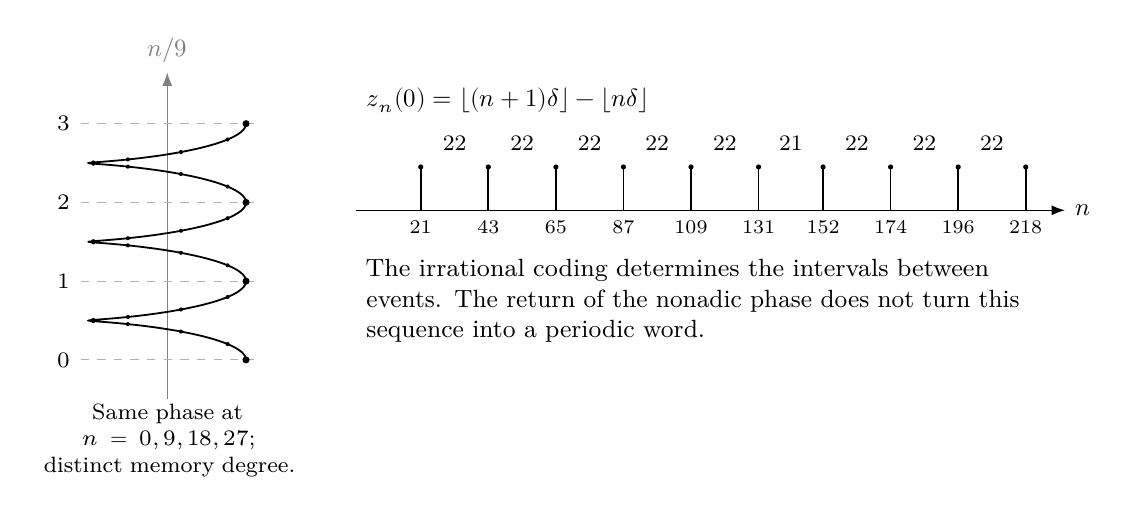
\begin{tikzpicture}[x=1cm,y=1cm,>=Latex,font=\small]
\begin{scope}[xshift=1.8cm,yshift=.3cm]
\draw[->,gray] (0,-.5)--(0,3.65) node[above] {\(n/9\)};
\foreach \k in {0,1,2,3}{
 \draw[gray!60,dashed] (-1.1,\k)--(1.1,\k);
 \node[left,font=\footnotesize] at (-1.1,\k){\(\k\)};
}
\draw[black,line width=.65pt,domain=0:27,samples=260,smooth,variable=\n]
 plot ({cos(40*\n)},{\n/9+.14*sin(40*\n)});
\foreach \n in {0,...,27}{
 \fill ({cos(40*\n)},{\n/9+.14*sin(40*\n)}) circle (.026);
}
\foreach \k in {0,1,2,3}{\fill (1,\k) circle (.045);}
\node[align=center,text width=3.3cm,font=\footnotesize] at (0,-1.02)
 {Same phase at \(n=0,9,18,27\);\\distinct memory degree.};
\end{scope}
\begin{scope}[xshift=4.2cm,yshift=.5cm]
\node[anchor=west] at (0,3.1){\(z_n(0)=\lfloor(n+1)\delta\rfloor-\lfloor n\delta\rfloor\)};
\draw[->] (0,1.7)--(9,1.7) node[right]{\(n\)};
\foreach \n in {21,43,65,87,109,131,152,174,196,218}{
 \draw[line width=.6pt] ({\n*.039},1.7)--({\n*.039},2.25);
 \fill ({\n*.039},2.25) circle (.033);
 \node[below,font=\scriptsize] at ({\n*.039},1.7){\n};
}
\foreach \a/\b/\g in {21/43/22,43/65/22,65/87/22,87/109/22,109/131/22,131/152/21,152/174/22,174/196/22,196/218/22}{
 \node[font=\footnotesize] at ({(\a+\b)*.0195},2.55){\g};
}
\node[anchor=west,align=left,text width=8.3cm] at (0,.55)
 {The irrational coding determines the intervals between events. The return of the nonadic phase does not turn this sequence into a periodic word.};
\end{scope}
\end{tikzpicture}
\caption{Two complementary representations of transport. On the left, the helix \((\cos(2\pi n/9),\allowbreak\sin(2\pi n/9),\allowbreak n/9)\) is projected: after nine steps, the phase returns while the height increases. On the right, the first ten events of the lower word for \(\delta=\log_{10}(10/9)\) are shown, with exact spacings of \(21\) or \(22\). The helical representation introduces no additional physical metric.}
\label{fig:holonomia-esturmiana}
\end{figure}


For this count, fix the intercept and the cumulative endpoints
\[
 \theta=0,\qquad
 (N_0,\ldots,N_4)=(0,729,972,999,1000),
\]
corresponding to the cubic order \((729,243,27,1)\). The lower and upper
counts are given by
\[
 c_j^-:=\lfloor N_j\delta\rfloor-\lfloor N_{j-1}\delta\rfloor,
 \qquad
 c_j^+:=\lceil N_j\delta\rceil-\lceil N_{j-1}\delta\rceil,
\]
and, with the same initial zero boundary, satisfy
\[
 (c_1^-,\ldots,c_4^-)=(33,11,1,0),\qquad
 (c_1^+,\ldots,c_4^+)=(34,11,1,0).
\]
These values depend on the intercept and the ordering of the strata; they are
not asserted for an arbitrary initial phase. Their totals are forty-five and
forty-six. The increment corresponds to a single boundary unit, located in
the first stratum of this ordered partition. The numbers thirty-four and
eleven thus appear in a single count prior to any unit chart; identifying them
with physical exponents also requires the corresponding dimensional derivation.

The designation \emph{aperiodic crystal} is used here for this symbolic order, with specified complexity, spectrum, and return. Zero topological entropy does not by itself amount to zero physical dissipation: a thermodynamic realization requires a defined energetic dynamics and erasure operation. Likewise, this Sturmian reading does not replace all TPK operators, nor does it by itself prove the periodicity or aperiodicity of the complete output of \(\alpha\). Its function is to make explicit an order structure that the calendar's simple return does not describe.

% Cumulative addition. Insert after the existing Sturmian suspension.
% Preserve the text and Figure fig:holonomia-esturmiana in full.
\subsection{Nonadic connection, holonomy, and monodromic representation}
\label{mono-ampl:conexion}

The regional connection already constructed is now studied through three
objects: transport of the complete state, representation of its turns, and
suspension of its itineraries. The APP--TRIT--TPK operations and the initial
catalog preserve the preceding definitions. The necessary distinction here
concerns what each representation retains from the same history, with all
required operations incorporated into this section.

At prolongation index \(k\), a chart of the state preserves
\[
 \widehat x_k=(B_k,C_k,p_k,c_k,\Sigma_k,W_k,g_k,m_k).
\]
Here \(B_k\) assembles the three regional blocks, \(C_k\) is the cylinder,
\(p_k\) the prefix, \(c_k\) the carry record, \(\Sigma_k\) the boundary
signature, and \(W_k\) the incidence information. The phase is
\(g_k=1+[(k-1)]_9\); \(m_k\) counts the complete turns. The reduction
\(\beta_k=[m_k]_{12}\) preserves the dodecaphase position, while the
integer \(m_k\) distinguishes its successive turns.

\begin{definition}[Transport through one nonadic turn]
\label{mono-ampl:def-vuelta}
Let \(\mathcal R_k\subseteq\widehat X_k\times\widehat X_{k+1}\)
be the admissible extension relations of the TPK. The realization of the
holonomy at level \(k\) is the relational composition
\[
 \Gamma_{9,k}=\mathcal R_{k+8}\circ\cdots\circ\mathcal R_k.
\]
For \(s\geq1\), its prolongation to \(s\) turns is
\[
 \Gamma_{9s,k}=
 \Gamma_{9,k+9(s-1)}\circ\cdots\circ\Gamma_{9,k}.
\]
\end{definition}

The relational formulation preserves the admissible continuations. On an
individualized history, each arrow leads to the state actually prolonged;
the isolated visible block may continue to admit more than one continuation.
This difference is precisely the function of memory and of the boundary
conditions in determining the path.

\begin{proposition}[Iteration of the return and accumulated memory]
\label{mono-ampl:vueltas}
In every admissible composition of \(s\) turns,
\[
 g_{k+9s}=g_k,\qquad m_{k+9s}=m_k+s,\qquad
 \beta_{k+9s}=\beta_k+s\pmod{12}.
\]
\end{proposition}
\begin{proof}
The one-turn rule preserves the phase and increments the counter by one.
Its application to the already transported state repeats exactly those two
operations. Induction gives the first two equalities; reducing the second
modulo \(12\) gives the third.
\end{proof}

The counter thus provides an integral witness to the difference between
turns. After \(12\) turns the pair of finite phases is restored, but the
counter increases by \(12\). The nonsplit extension
\eqref{eq:extension108} expresses the composition of the calendar through
its cocycle; the path also preserves the integral lift of that datum.
Preservation here means transport of the preceding contributions, not
immobility of all coordinates.

\subsubsection{Bilateral representation of the return index}

The shift \(T\) of \eqref{eq:weyl-relojes} admits an expression in
phase and turn coordinates. Number the phases from \(0\) to \(8\), by
shifting the origin relative to \(g_k\), and write \(k=9m+r\), with
\(0\leq r<9\), on the integer line covering the phase cycle. On
\(\mathcal H_{\rm ind}=\ell^2(\mathbb Z)\), the basis
\(|k\rangle=|r,m\rangle\) expresses that same unit shift
\[
 T|r,m\rangle=
 \begin{cases}
 |r+1,m\rangle,&r<8,\\
 |0,m+1\rangle,&r=8.
 \end{cases}
\]
The inverse decreases \(r\) by one when \(r>0\), and sends
\(|0,m\rangle\) to \(|8,m-1\rangle\). Passage through the phase origin
therefore incorporates the exact quotient unit.

\Needspace{8\baselineskip}
\begin{proposition}[Representation of the cycle monodromy]
\label{mono-ampl:representacion}
Let \(S=T^9\). Then
\[
 S|r,m\rangle=|r,m+1\rangle,\qquad
 \mathbb Z\longrightarrow\mathcal U(\mathcal H_{\rm ind}),
 \quad s\longmapsto S^s
\]
is a faithful unitary representation of the group of turns of the cycle.
\end{proposition}
\begin{proof}
Nine shifts preserve the remainder upon division by \(9\) and increment
the quotient. The powers satisfy \(S^{s+t}=S^sS^t\), and
\(S^s|r,m\rangle=|r,m+s\rangle\) distinguishes every integer \(s\).
A permutation of an orthonormal basis is unitary.
\end{proof}

This representation corresponds to the covering of the cycle, whose group
of turns is \(\mathbb Z\), and represents the phase together with its
counter. The TPK state also contains the path coordinates already described.
The bilateral extension admits negative indices as coordinates of the
covering; a path begun at an initial condition uses its admissible half-axis.
This provides an operator inverse for the index without turning each
extension relation into a bijection of the complete state.

With \(D_M|k\rangle=\lfloor k/9\rfloor|k\rangle\), the identity
\([D_M,S]=S\) expresses the increment of memory on the dense domain of
finite-support vectors. If \(\mathcal I|k\rangle=|-k\rangle\) and
\(P_0\) projects onto indices divisible by \(9\), one also obtains
\begin{equation}
 \mathcal I T\mathcal I=T^{-1},\qquad
 \mathcal I D_M\mathcal I=-D_M-(I-P_0).
 \label{mono-ampl:inversion-contador}
\end{equation}
Indeed, for \(k=9m+r\),
\(\lfloor-k/9\rfloor=-m\) if \(r=0\), and equals \(-m-1\) if \(r>0\).
The inversion thus preserves the boundary term of Euclidean division.

\subsection{Block clock and capacity clock}
\label{mono-ampl:relojes}

The index of a refinement mapping and the number of available decimal
positions obey related but different laws. To express them, reserve \(n\)
for the index of ternary blocks and define
\[
 \rho=\log_{1000}729=\log_{10}9,\qquad
 \delta=1-\rho,\qquad
 \mathcal C_n=\lfloor(n+1)\rho\rfloor,\quad n\geq0.
\]
Here the letter \(\mathcal C_n\) designates capacity, not the dodecaphase
record \(K\). At the canonical phase origin, the preceding mechanical word
gives
\[
 Z_n=\sum_{j=0}^{n}z_j(0)=\lfloor(n+1)\delta\rfloor.
\]

\begin{proposition}[Exact balance between capacity and vacancies]
\label{mono-ampl:balance-capacidad}
For \(n\geq0\), and in the second identity \(n\geq1\),
\[
 \mathcal C_n=n-Z_n,\qquad
 \mathcal C_n-\mathcal C_{n-1}=1-z_n(0).
\]
\end{proposition}
\begin{proof}
The irrationality of \(\delta\) implies
\(\lceil(n+1)\delta\rceil=\lfloor(n+1)\delta\rfloor+1\).
Then
\[
 \lfloor(n+1)(1-\delta)\rfloor
 =n+1-\lceil(n+1)\delta\rceil=n-Z_n.
\]
Subtracting two consecutive identities completes the proof.
\end{proof}

An event \(z_n=1\) adds a block to the history while retaining capacity
\(\mathcal C_n\); an event \(z_n=0\) increments both counters. On any
interval, the capacity increments and the vacancies sum to exactly its
length. Reducing modulo \(q\), for \(q=9\) or \(q=108\), gives
\[
 [\mathcal C_n]_q=[n]_q-[Z_n]_q.
\]
The uniform block phase and the capacity phase are related through the
integrated memory of vacancies. In particular, a capacity retention and a
complete turn of the connection have distinct mechanisms, although both may
preserve a phase observation.

The monotone inversion of the clock gives a first-arrival time:
\[
 T_{\rm cap}(a)=\min\{n:\mathcal C_n=a\}
 =\left\lceil\frac a\rho\right\rceil-1,
 \qquad a\geq1.
\]
With \(\sigma=\rho^{-1}-1\), the time required to gain \(b\) units of
capacity is
\[
 T_{\rm cap}(a+b)-T_{\rm cap}(a)
 =b+\lceil(a+b)\sigma\rceil-\lceil a\sigma\rceil.
\]
The difference of ceilings takes one of the two integers adjacent to
\(b\sigma\). Thus \(9\) or \(10\) blocks are obtained to gain
\(9\) units of capacity, and \(113\) or \(114\) to gain \(108\).
These are times of the inverse clock, measured from a first arrival; the
turn counter is always interpreted in the index to which it belongs.

\subsection{Symbolic suspension and aperiodic time crystal}
\label{mono-ampl:cristal}

The rotation coding brings together phase periodicity, local recurrence,
and global aperiodicity. Let \(\mathcal X_\delta\subseteq\{0,1\}^{\mathbb Z}\)
be the closure, in the product topology, of the translates of the bilateral
word \(z_n(\theta)\). Denote by \(\sigma_{\rm sh}\) the shift of its
sequences. Preserving a nonadic phase, the step is
\[
 F(r,z)=([r+1]_9,\sigma_{\rm sh}z),\qquad
 (r,z)\in C_9\times\mathcal X_\delta.
\]

\begin{definition}[Symbolic aperiodic time crystal]
\label{mono-ampl:def-cristal}
The unit-roof suspension of the preceding system is the space
\[
 \mathcal S_\delta=
 \bigl((C_9\times\mathcal X_\delta)\times\mathbb R\bigr)/\sim,
 \qquad (y,t+1)\sim(Fy,t),
\]
with flow \(\Phi_s[y,t]=[y,t+s]\). This model of temporal order, together
with its vacancy coding and the representation of the turn counter, is
called a \emph{symbolic aperiodic time crystal}.
\end{definition}

The adjective temporal designates the action of the flow and its return
section; aperiodicity characterizes its itineraries. The frequency of ones
in each sequence is \(\delta\): the uniform discrepancy bound below one,
obtained by telescoping on any window, persists upon taking the closure.
A periodic sequence would have rational frequency. Therefore,
\(\mathcal X_\delta\) contains no periodic orbits. The suspension likewise
has no closed orbits: a return of the flow would require an integer time and
periodicity of the itinerary.

Finite words do recur. The itineraries of length \(m\) arise from a
partition of the circle by \(m+1\) points; every interval is visited
recurrently by the irrational rotation. Even when times are restricted to a
fixed phase, the step \(9\delta\) remains irrational. This is why every word
appears in all \(9\) phases and why the already established complexities are
\[
 p(m)=m+1,\qquad p_9(m)=9(m+1),\qquad p_3(m)=3(m+1).
\]
The recurrence of local configurations coexists with the absence of a global
period. Its topological entropy is zero because these complexities grow
linearly.

The realization through the observables \(V_9,W_\delta\) and the shift
\(T\) expresses the same order through the covariances
\eqref{eq:weyl-relojes}. The frequencies of the uniform clock belong to
\(\frac19\mathbb Z+\delta\mathbb Z\), modulo \(1\). The capacity clock
additionally preserves the relation
\([\mathcal C_n]_9=[n]_9-[Z_n]_9\); it is not replaced by the uniform phase
when interpreting the returns. The term \emph{time crystal} is thereby
defined through a mathematical dynamical system. Its physical realization
requires specification of an energetic dynamics, its temporal observables,
and its stability, data distinct from the present symbolic construction.

\subsection{Mirror symmetry of the regions and double realization}
\label{mono-ampl:regiones}

The mirror interchange acts on the regional block
\(B=(u^\pi,u^e,u^\varphi)\in(\mathbb F_3^6)^3\) by
\[
 \mathfrak cB=(u^e,u^\pi,u^\varphi).
\]
Its fixed axis and its aggregate are, respectively, \(u^\varphi\) and
\(s=u^\pi+u^e\). This fixing refers to the involution in one fiber;
both coordinates may evolve during nonadic transport.
With \(q=u^\pi+u^e+u^\varphi\),
\(a=u^\pi+u^e-u^\varphi\), and \(d=u^\pi-u^e\), one recovers
\[
 u^\varphi=2(q-a),\qquad s=q-u^\varphi,\qquad
 u^\pi=2(s+d),\qquad u^e=2(s-d).
\]
The equalities hold componentwise in \(\mathbb F_3\), where
\(2^{-1}=2\). The mirror preserves \(q,a,s\) and reverses \(d\); this
antisymmetric coordinate individualizes the distribution that the aggregate
preserves without distinguishing. The inversion \(\mathcal I\) of the
temporal index and the channel involution \(\mathfrak c\) therefore act on
different data.

The phase return has an explicit witness:
\[
 \begin{aligned}
 B_1&=(012222\mid121221\mid112202),\\
 B_{10}&=(101222\mid112221\mid112002).
 \end{aligned}
\]
The two positions have phase \(1\); the block, the axis, and the memory have
changed. Likewise, synchronization of the censuses in phases \(8\) and
\(9\) annihilates their relative differences, while the diagonal component
passes from \((59,59,59)\) to \((43,43,43)\). Equality of a relative
observable does not exhaust the state that determines it.

The double realization preserves that architecture. In Section
\ref{exc:doble-lectura}, the same prefix determines nested cylinders on the
one hand and a sequence of encoded words with their frames on the other.
The first map passes to the limit by contraction of diameters; the second
satisfies \(r_{n,m}Q_n=Q_mp_{n,m}\) and defines \(Q_\infty\).
Figure \ref{mono-ampl:fig-regional} anticipates these two mappings.
The subsequent incidence path constructs codes, lattices, and the Moonshine
realization in their own domains; the automorphism group acts on that
realization, not on the digits through an implicit identification.

% Cumulative figure; destination figures/monodromia_regional_ampliacion.tex.
\begin{figure}[H]
\centering
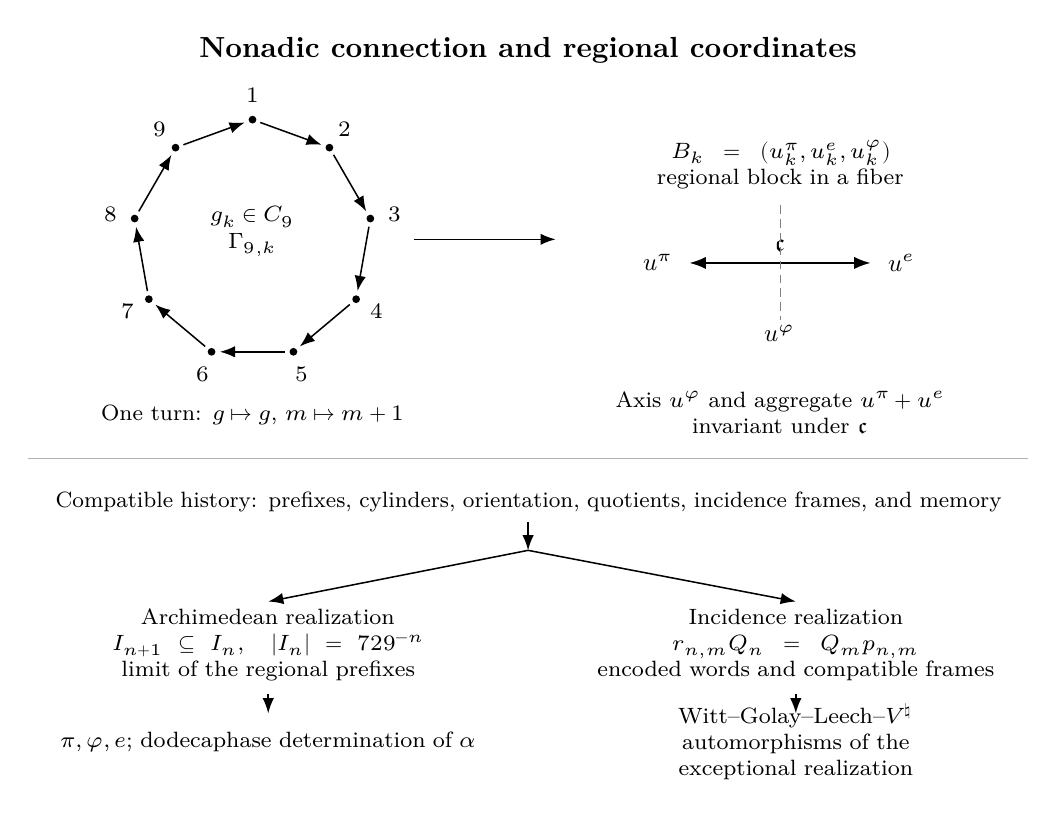
\begin{tikzpicture}[x=1cm,y=1cm,>=Latex,font=\small,
  flow/.style={->,line width=.55pt},
  ann/.style={align=center,font=\footnotesize}]
\node[font=\bfseries] at (6.9,9.2)
  {Nonadic connection and regional coordinates};
\begin{scope}[shift={(3.4,6.8)}]
 \foreach \k in {1,...,9}{
  \pgfmathsetmacro{\ang}{90-40*(\k-1)}
  \coordinate (p\k) at (\ang:1.52);
  \fill (p\k) circle (1.4pt);
  \node[fill=white,inner sep=1.1pt,font=\footnotesize]
    at (\ang:1.83) {\(\k\)};
 }
 \foreach \k in {1,...,8}{
  \pgfmathtruncatemacro{\next}{\k+1}
  \draw[flow,shorten >=3pt,shorten <=3pt] (p\k)--(p\next);
 }
 \draw[flow,shorten >=3pt,shorten <=3pt] (p9)--(p1);
 \node[ann] at (0,.1) {\(g_k\in C_9\)\\\(\Gamma_{9,k}\)};
 \node[ann] at (0,-2.23) {One turn: \(g\mapsto g\), \(m\mapsto m+1\)};
\end{scope}
\node[ann,text width=5.25cm] at (10.1,7.75)
 {\(B_k=(u_k^\pi,u_k^e,u_k^\varphi)\)\\
 regional block in a fiber};
\node at (8.55,6.5) {\(u^\pi\)};
\node at (11.65,6.5) {\(u^e\)};
\draw[<->,line width=.65pt] (8.95,6.5)--node[above]{\(\mathfrak c\)}(11.25,6.5);
\draw[densely dashed,gray] (10.1,5.72)--(10.1,7.23);
\node[fill=white,inner sep=2pt] at (10.1,5.6){\(u^\varphi\)};
\node[ann] at (10.1,4.6)
 {Axis \(u^\varphi\) and aggregate \(u^\pi+u^e\)\\
 invariant under \(\mathfrak c\)};
\draw[flow] (5.45,6.8)--(7.25,6.8);
\draw[gray!60,line width=.3pt] (.55,4.02)--(13.25,4.02);
\node[ann,text width=12cm] (hist) at (6.9,3.47)
 {Compatible history: prefixes, cylinders, orientation, quotients,
 incidence frames, and memory};
\coordinate (fork) at (6.9,2.85);
\draw[flow] (hist.south)--(fork);
\draw[flow] (fork)--(3.6,2.2);
\draw[flow] (fork)--(10.3,2.2);
\node[ann,text width=5.6cm] at (3.6,1.65)
 {Archimedean realization\\
 \(I_{n+1}\subseteq I_n,\quad |I_n|=729^{-n}\)\\
 limit of the regional prefixes};
\node[ann,text width=5.6cm] at (10.3,1.65)
 {Incidence realization\\
 \(r_{n,m}Q_n=Q_mp_{n,m}\)\\
 encoded words and compatible frames};
\node[ann,text width=5.6cm] at (3.6,.42)
 {\(\pi,\varphi,e\); dodecaphase determination of \(\alpha\)};
\node[ann,text width=5.6cm] at (10.3,.42)
 {Witt--Golay--Leech--\(V^\natural\)\\
 automorphisms of the exceptional realization};
\draw[flow] (3.6,1.03)--(3.6,.78);
\draw[flow] (10.3,1.03)--(10.3,.78);
\end{tikzpicture}
\caption{\fontsize{9}{11}\selectfont Nine phases of a connection and two realizations of the compatible
history. The cycle represents the phase; each turn increments the counter.
The regional diagram represents the involution \(\mathfrak c\), which
interchanges closure and propagation and fixes the self-scaling axis in a fiber.
This invariance does not impose that the axis remain constant during transport.
The two lower mappings use the same prefix: one determines its numerical
limit, and the other preserves words and incidence frames. The maps of this
second realization are specified in Section \ref{exc:doble-lectura}; the
exceptional path is developed subsequently.}
\label{mono-ampl:fig-regional}
\end{figure}


\Needspace{30\baselineskip}
\subsubsection{Linear representation of the phases and the return}
\label{mono-recta:desarrollo}

The representation on the segment \([0,10]\) preserves the positional
origin of APP and orders its nine interior marks. In this diagram,
the integers \(1,\ldots,9\) are phase representatives. The horizontal
position indicates the order of the charts; the upper labels specify
regional operations. Figure \ref{mono-recta:figura} thus brings together
the initial real line, the fixing of the self-scaling axis, the mirror
distribution of the two channels, and the return with memory developed
in the preceding construction.

\input{figures/recta_nonadica_0_10.tex}

The fixing of the axis is formulated in the fiber of a given boundary. If
\(q=u^\pi+u^e+u^\varphi\) and
\(a=u^\pi+u^e-u^\varphi\), then
\[
 u^\varphi=2(q-a),\qquad s=u^\pi+u^e=q-u^\varphi
 \quad\text{in }\mathbb F_3^6.
\]
The data \((q,a)\) determine the axis and the aggregate; the ordered
distribution of \(s\) preserves the mirror freedom resolved by the
prolongation. The fifth phase has a local solution and an extension, with
boundary datum \(c=111111\) and residual signature \(\rho_W=000\). This is
the meaning of its first strong saturation. The symbol \(\varphi\)
placed above mark \(5\) identifies the regional axis that enters
that operation.

The intermediate phases preserve this decomposition within each fiber,
while their boundary data evolve. The complete census of local
multiplicities and extensions of the distinguished branch is
\[
\begin{array}{c|rrrrrrrrr}
\text{phase}&1&2&3&4&5&6&7&8&9\\\hline
N_{\rm loc}&3&2&5&4&1&1&3&3&2\\
N_{\rm ext}&2&5&4&1&1&3&3&2&1
\end{array}
\]
Phase \(6\) combines local uniqueness and three prolongations; phase
\(7\) resolves a triple mirror fiber; phase \(8\) synchronizes
the three regional censuses. Phase \(9\) preserves two local
distributions with the same axis and the same aggregate, one of which
is prolonged. These counts express different functions within a
single connection and justify the marks on the real line.

In particular, for phases \(6,7,8\), the regional sums are
respectively \(012100\), \(101001\), and \(112000\). The preservation
represented by the brace is an invariance with respect to the mirror
distribution in each fiber. The subsequent real evaluation applies the
readers of the compatible cylinders to the complete histories; the
internal sum represented in the figure belongs to the ternary domain.

Finally, the arc \(9\to1\) represents passage from one turn to the
next. The formulas in Section \ref{mono-ampl:conexion} preserve the
phase remainder and increment the turn counter. The linear diagram and
the cyclic diagram in Figure \ref{mono-ampl:fig-regional} therefore
express two complementary aspects of the same holonomy: the ordering of
positions and the composition of the return on the state with memory.


\subsection{Temporal transport and tritic exponential composition}
\label{mono-ampl:euler}

The Euler relations in Section \ref{euler-trit-articulacion}
describe the local realizations of the three regimes. For a fixed signature
\(\tau\), the generator satisfies \(J_\tau^2=-\tau I\); algebraic
conjugation sends \(J_\tau\) to \(-J_\tau\). Consequently,
\[
 \exp(sJ_\tau)\exp(tJ_\tau)=\exp((s+t)J_\tau),\qquad
 \overline{\exp(tJ_\tau)}=\exp(-tJ_\tau),
\]
and the product of an evolution with its conjugate is the unit. In the
elliptic type it is realized through \(\cos^2t+\sin^2t=1\); in the
hyperbolic type, through \(\cosh^2t-\sinh^2t=1\); in the parabolic type,
\((I+tN)(I-tN)=I\), since \(N^2=0\). The same conservation law admits
three quadratic expressions.

The elliptic realization closes a turn; the nilpotent one preserves a linear
shift; the hyperbolic one separates expansion and contraction with unit
determinant. At the regional parameters already generated,
\[
 \exp(\pi J_{\mathrm e})=-I,\qquad
 \exp(J_{\mathrm p})=I+J_{\mathrm p},\qquad
 \exp(2\log\varphi\,J_{\mathrm h})=F_{\rm av}^{\,2}.
\]
The evaluation \(\exp(I)=eI\) recognizes the unit of the common exponential
law. The number \(e\) is not assigned exclusively to the parabolic regime.

Transport of a local realization by an isomorphism \(U\) preserves these
relations: if \(J'=UJU^{-1}\), the exponential series gives
\(U\exp(tJ)=\exp(tJ')U\). The identity transports the regime and its
norm. A transition between different quadratic types instead belongs to the
selection of TPK sheets and regimes; it is not a conjugation that changes
the value of \(J^2\). The temporal product therefore preserves the order of
the transitions and the information at their endpoints.

This articulation distinguishes the closure of a local representation from
the holonomy of a history. The equality \(\exp(2\pi J_{\mathrm e})=I\)
may hold at the same time as \(S|r,m\rangle=|r,m+1\rangle\). The first
equality restores the orientation of the regime; the second records another
turn. The discrete structure preserves both: the local return and the
accumulated provenance of the state that realizes it.


% Recovery of the native product and its selector, not incorporation of RH.
\subsection{Multiplicative irreducibility and return periods}
\label{primos-retornos}

The distinction among structure, evaluation, and phase also appears in the
multiplicative sector. The local APP product contains both the remainder
and the quotient; its iteration makes it possible to construct normal forms
and factorizations before examining their decimal periods. This development
places the expression \emph{prime mode} in a precise domain and relates
irreducibility to the operations already defined, not to an isolated
coincidence of periods.

Let
\[
 \mathcal W_9=\{\varnothing\}\sqcup
 \bigsqcup_{\ell\geq1}\{1,\ldots,9\}^{\ell}.
\]
The sequences are ordered from the least significant digit. The evaluation
\(\operatorname{ev}_9(u)=\sum_j u_j9^j\), with
\(\operatorname{ev}_9(\varnothing)=0\), is bijective onto the nonnegative
integers: for a positive integer, division of \(n-1\) by \(9\)
uniquely determines the first digit and the continuation. This is the
bijective nonadic numeration; it preserves the representative \(9\) of the
boundary.

The sum \(\boxplus_\#\) is obtained by applying the additive sheet of APP to
the digits at each position and propagating their quotients. If there is only
one digit, it constitutes the provisional remainder; a nonzero incoming
quotient is normalized by a second additive operation. The sum of the
quotients is transported to the next position. To multiply a sequence by a
digit \(d\), the multiplicative cell produces \(u_jd=9q_j+r_j\), and the
incoming quotient \(c_j\) is incorporated through
\[
 (w_j,c_{j+1})=
 \begin{cases}
 (r_j,q_j),&c_j=0,\\
 \bigl(R^+(r_j,c_j),q_j+q^+(r_j,c_j)\bigr),&c_j>0.
 \end{cases}
\]
One begins with \(c_0=0\), and the final quotient is incorporated when it is
nonzero. During addition, \(c_j\leq2\); during multiplication by a digit,
\(c_j\leq9\). The local operations thus receive arguments within
their domain. Denote this second procedure by \(d\odot_\#u\),
with \(d\odot_\#\varnothing=\varnothing\).

For \(v=(v_0,\ldots,v_{m-1})\), the full product is constructed by
the recurrence
\[
 a_m=\varnothing,\qquad
 a_j=(9\odot_\#a_{j+1})\boxplus_\#(v_j\odot_\#u),
 \qquad u\boxtimes_\#v=a_0.
\]
The rule composes the two local sheets. Its evaluation verifies
\begin{equation}
 \operatorname{ev}_9(u\boxtimes_\#v)
   =\operatorname{ev}_9(u)\operatorname{ev}_9(v).
 \label{eq:primos-entrelazamiento}
\end{equation}
Indeed, each transition preserves the partial sum plus the pending quotient
weighted by the corresponding power of \(9\). The recurrence then gives
\(\operatorname{ev}_9(a_j)=9\operatorname{ev}_9(a_{j+1})+
v_j\operatorname{ev}_9(u)\), whose iteration proves
\eqref{eq:primos-entrelazamiento}. The uniqueness of the normal form transports
associativity and commutativity to the constructed product; its unit is \((1)\).

\begin{definition}[Reduced multiplicative coproduct]
On the finite-support vector space generated by the nonempty normal
forms, define
\[
 \widetilde\Delta_\# e_w
 =\sum_{\substack{u\boxtimes_\#v=w\\u,v\ne(1)}}e_u\otimes e_v.
\]
A nonunit normal form is irreducible when its image under
\(\widetilde\Delta_\#\) is zero.
\end{definition}

The factorization fibers are finite by
\eqref{eq:primos-entrelazamiento}. In the completion
\(\mathcal H_\#=\ell^2(\mathcal W_9\setminus\{\varnothing\})\),
the images of distinct forms have disjoint supports. If
\(d_\#(w)\) counts the ordered nonunit factorizations, the domain
of the closure is
\[
 \operatorname{Dom}(\overline{\widetilde\Delta_\#})
 =\left\{x\in\mathcal H_\#:
       \sum_w d_\#(w)|x_w|^2<\infty\right\}.
\]
\Needspace{8\baselineskip}
Indeed, the squared norm of the image is that weighted sum. Therefore,
the operator
\[
 A_\#=(\overline{\widetilde\Delta_\#})^*
                  \overline{\widetilde\Delta_\#}
\]
is diagonal, positive, and self-adjoint: its eigenvalue at \(e_w\) is the
number of ordered nonunit factorizations of \(w\). The projection
\[
 P_{\rm irr}=(I-|e_{(1)}\rangle\langle e_{(1)}|)
                    \mathbf1_{\{0\}}(A_\#)
\]
selects exactly the irreducible forms. Through the multiplicative
evaluation, these correspond to the ordinary primes. The selection
depends on the factorization structure and keeps the unit state separate.

For a value \(n\geq2\) coprime to \(10\), decimal division induces the
permutation of remainders \(r\mapsto10r\pmod n\). The return of remainder
\(1\) has period
\[
 \tau_n=\operatorname{ord}_n(10).
\]
If \(n=\prod_p p^{a_p}\), the Chinese remainder theorem gives
\[
 \tau_n=\operatorname{lcm}_{p^{a_p}\parallel n}
                    \operatorname{ord}_{p^{a_p}}(10).
\]
The composite return synchronizes the returns of the prime powers.
For a prime \(p\notin\{2,3,5\}\), one has
\[
 \tau_p\mid p-1,\qquad
 M_p=\frac{10^{\tau_p}-1}{p}\in\mathbb N,
 \qquad M_p\equiv0\pmod9.
\]
The last congruence expresses the nonadic closure of the decimal repetition:
\(10^{\tau_p}-1\) is a multiple of \(9\), and \(p\) is invertible modulo
\(9\). The same congruence holds for every \(n\) coprime to
\(90\). In particular, \(7,13,77,91,143\) have decimal period \(6\),
although only the first two are irreducible. The coproduct and the period
therefore record different properties of the same constructed value.

This differentiation specifies the relation with aperiodic refinement.
The vacancy sequence determines the increments of the capacity index;
factorization determines the multiplicative modes; decimal division
determines their return times. The nonadic representative preserves phase
closure, whereas the quotient and factorization preserve information that
this closure does not distinguish. The link with the spectral constructions
of the treatise resides in those operators and their intertwining maps. The
proof of its subsequent analytic results retains its own development; it is
not replaced by the periodicity of a residual observation.

\subsubsection{Vacancy discrepancy and Dirichlet readings}

The link also admits an exact analytic expression. The same coding
\(z_n=z_n(0)\), for \(n\geq1\), is retained, and two subsequent
observables are considered: the series over all indices and the product
over the indices selected by irreducibility. For
\(\operatorname{Re}s>1\),
\[
 Z_{\rm vac}^{+}(s)=\sum_{n\geq1}\frac{z_n}{n^s},\qquad
 Z_{\rm vac}^{\times}(s)=\prod_p(1-p^{-s})^{-z_p}.
\]
Both converge absolutely in that half-plane. Their common factor is the
density \(\delta\), but their discrepancies are different.

\Needspace{21\baselineskip}
\begin{proposition}[Separation of the vacancy density]
One has
\[
 Z_{\rm vac}^{+}(s)=\delta\zeta(s)+H_{\rm vac}(s),
 \qquad H_{\rm vac}\in\mathcal O(\operatorname{Re}s>0).
\]
In \(\operatorname{Re}s>1\), with logarithms defined by the absolutely
convergent Euler series,
\[
 Z_{\rm vac}^{\times}(s)=\zeta(s)^\delta G_{\rm vac}(s),\qquad
 \log G_{\rm vac}(s)=
 \sum_p(z_p-\delta)\log(1-p^{-s})^{-1}.
\]
\end{proposition}
\begin{proof}
The centered partial sums satisfy
\[
 A_N:=\sum_{n=1}^N(z_n-\delta)
 =\lfloor(N+1)\delta\rfloor-N\delta,\qquad |A_N|<1.
\]
Abel summation represents the centered term by
\(s\int_1^\infty A_{\lfloor x\rfloor}x^{-s-1}\,dx\). The integral
converges locally uniformly in \(\operatorname{Re}s>0\),
which proves holomorphy. The second identity results from separating
\(z_p=\delta+(z_p-\delta)\) in the logarithm of the product, within
its domain of absolute convergence.
\end{proof}

The decomposition makes visible what the reading over primes adds: it
examines the same vacancy sequence on a subset determined by
factorization. Controlling the discrepancy over all integers gives
the first holomorphic continuation; the second observable preserves a
discrepancy of its own over primes. These are two applications of the same
discrete structure, with explicit analytic domains. This articulation
establishes its relevance to the arithmetic core without transferring to
this article the proof of the terminal results of the treatise.



\clearpage
\section{Proof of \texorpdfstring{\(2^{\aleph_0}=\aleph_1\)}{2 to the power aleph zero equals aleph one} in the HMT continuum}
\label{sec:cierre-cardinal-nativo}

This section brings together, in a contiguous proof, extension, double
projection, and arbitrary depth; it then constructs the semantic closure,
the uniform lift, the genealogical machinery, and the cardinal closure. The
set-theoretic hierarchy is identified only at the end of the construction and
cannot be read as its causal origin. The causal dependence is:

\[
 \mathrm{APP}\longrightarrow\mathrm{TRIT}\longrightarrow\mathrm{TPK}
 \longrightarrow X_\infty^{\rm enr}
 \longrightarrow\mathcal C_{\rm cont}^{\rm disc}
 \longrightarrow m_\infty
 \longrightarrow\mathfrak G_{\rm HMT}(h,m_\infty).
\tag{32}\label{eq:ch-cadena-causal}
\]

First, the state, its extensions, the continuum, and the genealogical ledger
are constructed. Then \textbf{that produced genealogy} is extended to all its
hereditary objects by an explicit semantic rule. The subsequent identification
with a known set-theoretic hierarchy selects neither the seeds, the operators,
the genealogical ledger, the line, nor its projections. It does, however,
permit the exact logical-cardinal strength of the adopted semantic rule to be
assessed with complete transparency.

\subsection{Extension of states and transfinite semantic extension}

Let

\[
 \Sigma_{\rm HMT}
 =\bigl(\dot R_{\rm APP},\dot R_{\rm TRIT},\dot R_{\rm TPK},
 \dot R_{U},\dot R_{\Gamma_9},\dot R_{\rm Ext},\dot R_\rho,
 \dot R_{\pi},\dot R_{\varphi},\dot R_e,\dot R_{\alpha},
 \dot R_{\rm ar},\dot R_{\rm exc}\bigr)
\tag{33}\label{eq:ch-signatura}
\]

be the countable \textbf{relational} signature whose effective code is \(h\).
Each \(\dot R_S\) is the graph of the operator \(S\) on the codes where it is
defined; no external function is assumed to be total within each level. The
graphs \(\dot R_{\pi},\dot R_{\varphi},\dot R_e,\dot R_{\alpha}\) are the
output readers constructed by coinductive generation and dodecaphase closure;
they do not take the conventional values of the constants as arguments. Their
presence in \(\Sigma_{\rm HMT}\) ensures that the closure preserves the full
state: it simultaneously integrates the routes that express value and the
incidence that extends toward the exceptional realization.

At each horizon, the state code records the APP--TRIT--TPK coordinates, the
route, sheet, carry, boundary, and memory; at its representation stages it also
records \(P_N,\Phi_N,E_N,A_N\), where \(A_N\) is the prefix of
\(\alpha_{\rm HMT}\) produced by the same state. These coordinates do not
select the branch from outside: they are part of the history being encoded.
Once a primitive-recursive numbering of the finite coordinates of a state is
fixed, every inverse history
\(x_\infty=(x_N)_{N\geq1}\in X_\infty^{\rm enr}\) determines the code
\[
 \operatorname{code}(x_\infty)
 :=\{\langle N,j,c\rangle:(x_N)_j\text{ has code }c\}\subseteq\omega.
\]
The coherence equations
\(\rho_{N+1,N}(x_{N+1})=x_N\) make it possible to decode the history uniquely
from that real. We write \(m_\infty\) for the code of the realized history and
\(m_\infty(n)\) for its characteristic function under the fixed numbering.
The operator code \(h\) and this complete ledger are combined, by means of a
primitive-recursive pairing function, into the real

\[
 u_{h,m}:=
 \{\langle0,\langle n,h(n)\rangle\rangle:n<\omega\}
 \cup
 \{\langle1,\langle n,m_\infty(n)\rangle\rangle:n<\omega\}.
\tag{33a}\label{eq:ch-codigo-conjunto}
\]

The two primitive projections recover \(h\) and \(m_\infty\) from
\(u_{h,m}\).

The first extension is the metric and operator extension of the finite states.
For \(N\ge1\), let \(\widehat{\mathcal X}^{\rm enr,raw}_{6N}\) be the set of
raw enriched states of length \(6N\), and define the surviving subsystem
set-theoretically by
\[
\begin{aligned}
 X_N
 &:=\widehat{\mathcal X}^{\rm enr,surv}_{6N}\\
 &:=\Bigl\{x\in\widehat{\mathcal X}^{\rm enr,raw}_{6N}:\\[-.2ex]
 &\qquad\forall M>N\ \exists z\in
   \widehat{\mathcal X}^{\rm enr,raw}_{6M}\;\text{ such that}\\[-.2ex]
 &\qquad\operatorname{tr}_{6M,6N}(z)=x\ \wedge\
   z\text{ satisfies every intermediate TPK transition}\Bigr\}.
\end{aligned}
\]
and set
\[
 \rho_{N+1,N}:=\operatorname{tr}_{6N+6,6N}\!\upharpoonright X_{N+1},
\]
and
\[
 \operatorname{Ext}_N(x):=
 \{y\in X_{N+1}:(x,y)\in
 \operatorname{Ext}_{6N+6,6N}\}.
\]
The root level is included without any implicit exception:
\[
 X_0:=\{\ast\},\qquad
 \rho_{1,0}:X_1\to X_0\text{ is constant},\qquad
 \operatorname{Ext}_0(\ast):=X_1.
\]
The superscript \(\mathrm{surv}\) denotes the pruned tree of states possessing
compatible TPK descendants at every finite horizon. The TPK extension law
established in the preceding sections proves that the emitted seeds belong to
this tree; finite branching and Kőnig's lemma turn compatibility at every
horizon into an infinite branch. In particular,

\[
 \forall N\ge0\;\forall x\in X_N\quad
 \varnothing\ne\operatorname{Ext}_N(x)
 \subseteq\rho_{N+1,N}^{-1}(x).
\tag{34}\label{eq:ch-extension-no-vacia}
\]

By the same finitely branching tree lemma, every surviving seed has a
compatible extension

\[
 x_\infty=(x_N)_{N\ge1}\in
 X_\infty^{\rm enr}:=\varprojlim_N(X_N,\rho_{N+1,N}).
\tag{35}\label{eq:ch-limite-inverso}
\]

The second extension acts \textbf{afterward} on the complete code of that
realized history. It is not inferred from the mere existence of the finite
operator \(\operatorname{Ext}_N\): at set-theoretic scale it formalizes the
HMT principle that the only objects in the entire domain are those having a
genealogical derivation from the state and its rules. The transfinite semantic
extension is:

\[
 \begin{aligned}
  \mathfrak G_0(h,m_\infty)
  &:=\operatorname{TC}\bigl(\{\omega,u_{h,m},h,m_\infty\}\bigr),\\
  \mathfrak G_{\beta+1}(h,m_\infty)
  &:=\operatorname{Def}_{\Sigma_{\rm HMT}}
       \bigl(\mathfrak G_\beta(h,m_\infty)\bigr),\\
  \mathfrak G_\lambda(h,m_\infty)
  &:=\bigcup_{\beta<\lambda}\mathfrak G_\beta(h,m_\infty)
       \quad(\lambda\text{ limit}),\\
  \mathfrak G_{\rm HMT}(h,m_\infty)
  &:=\bigcup_{\beta\in\operatorname{Ord}}
       \mathfrak G_\beta(h,m_\infty).
 \end{aligned}
\tag{36}\label{eq:ch-clausura-transfinita}
\]

The Continuum Hypothesis and a target bijection are not introduced among the
conditions defining the successor operator; the operator is given
prospectively by

\[
 \operatorname{Def}_{\Sigma_{\rm HMT}}(M)
 :=M\cup
 \Bigl\{
   \{x\in M:\langle M,\in,
       (\dot R_S\cap M^{k_S})_{S\in\Sigma_{\rm HMT}}\rangle
       \models\varphi(x,\bar p)\}:
   \ulcorner\varphi\urcorner\in\omega,
   \ \bar p\in M^{<\omega}
 \Bigr\}.
\tag{37}\label{eq:ch-operador-def}
\]

That is, it simultaneously expresses all subsets definable by a finite formula
of the HMT relational language and parameters already produced by the
genealogy. It consults neither a target real value, a conventional constant, a
target cardinal, nor an external model. Formula~\eqref{eq:ch-operador-def}
defines the transfinite closure over the previously constructed seeds,
operators, enriched state, ledger, and double projection.

\begin{lemma}[Joint coding of the HMT program and the realized ledger]
\label{thm:ch-6}
The pair formed by the operator code \(h\) and the ledger \(m_\infty\) is
encoded by a single real \(u_{h,m}\subseteq\omega\), and every formula of
\(\Sigma_{\rm HMT}\) is uniformly translated into a formula of the language
\(\{\in,u_{h,m}\}\).

\end{lemma}
\begin{proof}
Both \(h\) and \(m_\infty\) are sequences of natural numbers: \(h\) encodes
the signature, the finite tables, and the operator programs; \(m_\infty\)
encodes one realized history, not the complete history space.
Formula~\eqref{eq:ch-codigo-conjunto} and its two decoders prove the first
assertion. Each symbol in~\eqref{eq:ch-signatura} denotes its \textbf{graph
relation encoded in \(h\)}, never the external graph of all its possible
evaluations. APP, TRIT, \(U_t\), \(\Gamma_9\), the restrictions \(\rho\), and
the finite extensions have primitive-recursive graphs on integer codes and,
therefore, \(\Delta_0\) formulas absolute between transitive levels. The two
representations are expressed as graph relations through the formulas

\[
 \begin{aligned}
 \dot R_{\rm ar}(x,y)
 &\;\Longleftrightarrow\;
 \forall k\in\omega\;\exists N\;\forall n\ge N\quad
 |\mu_n(x)-y|<2^{-k},\\
 \dot R_{\rm exc}(x,c,z)
 &\;\Longleftrightarrow\;
 \forall N\in\omega\quad z\!\upharpoonright N
   =E_N(x\!\upharpoonright N,c\!\upharpoonright N),
 \end{aligned}
\tag{37c$_0$}\label{eq:ch-grafos-publicacion}
\]

where \(\mu_n\) and \(E_N\) are the rational/finite functions whose codes
occur in \(h\). Every atomic formula containing an HMT symbol is inductively
replaced by its graph formula with parameter \(u_{h,m}\). Connectives and
quantifiers are preserved. This induction on syntactic complexity produces a
translation \(\varphi\mapsto\varphi^*\) such that, for every transitive level
\(M\) of~\eqref{eq:ch-clausura-transfinita} containing the parameters,

\[
 \langle M,\in,(\dot R_S\cap M^{k_S})_S\rangle
   \models\varphi(\bar a)
 \quad\Longleftrightarrow\quad
 M\models\varphi^*(\bar a;u_{h,m}).
\tag{37c}\label{eq:ch-eliminacion-uniforme}
\]

Thus, \eqref{eq:ch-operador-def} cannot consult an oracle, a target decimal
table, or an uncoded relation that introduces uncountably many objects in a
single step.
\end{proof}

HMT semantics is now defined \textbf{independently of identifying it with
\(\mathfrak G\)}. Let \(\mathcal T_0^{\rm HMT}\) be the set of canonical names
of the elements of
\(\mathfrak G_0(h,m_\infty)=
\operatorname{TC}(\{\omega,u_{h,m},h,m_\infty\})\). In particular, the
initial level contains the realized ledger \(m_\infty\), not every history
in \(X_\infty^{\rm enr}\) as primitive parameters. The admissible terms are
the well-founded trees obtained by

\[
 \begin{aligned}
 \mathcal T^{\rm HMT}_{\beta+1}
 &:={\mathcal T}^{\rm HMT}_\beta\cup
 \{\langle\beta,\ulcorner\varphi\urcorner,
       t_0,\ldots,t_{k-1}\rangle:
       t_i\in\mathcal T^{\rm HMT}_\beta\},\\
 \mathcal T^{\rm HMT}_\lambda&:=
       \bigcup_{\beta<\lambda}\mathcal T^{\rm HMT}_\beta,
 \qquad
 \mathcal T^{\rm HMT}:=
       \bigcup_{\beta\in\operatorname{Ord}}\mathcal T^{\rm HMT}_\beta.
 \end{aligned}
\tag{37a}\label{eq:ch-terminos}
\]

The value of a successor term is the subset of the preceding level defined by
\(\varphi\) in the induced relational structure, with the values of
\(t_0,\ldots,t_{k-1}\) as parameters. Before any set-theoretic comparison,
define

\[
 \operatorname{Ob}_{\rm sem}^{\rm HMT}(h,m_\infty)
 :=\{\llbracket t\rrbracket:t\in\mathcal T^{\rm HMT}\}.
\tag{37b}\label{eq:ch-objetos-semanticos}
\]

This is the rule of \textbf{generative exhaustivity} adopted by HMT: every
object in the entire domain must possess one of these derivation trees, and
every admissible tree expresses an object. It is not a consequence of finite
branching. The Continuum Hypothesis is not introduced into this rule; it is
obtained through the proof developed in the article. Neither an enumeration of
the reals nor a target bijection is introduced as data.

\begin{theorem}[Equivalence between term semantics and the genealogical hierarchy]
\label{thm:ch-6a}
The evaluation of the preceding terms satisfies

\[
 \operatorname{Ob}_{\rm sem}^{\rm HMT}(h,m_\infty)
 =\mathfrak G_{\rm HMT}(h,m_\infty).
\tag{37d}\label{eq:ch-equivalencia-semantica}
\]

\end{theorem}
\begin{proof}
By transfinite induction. At the initial level, the two classes coincide. If
every value of a term in \(\mathcal T^{\rm HMT}_\beta\) belongs to
\(\mathfrak G_\beta\), the semantics of a successor term is one of the subsets
in~\eqref{eq:ch-operador-def}. Conversely, every subset in
~\eqref{eq:ch-operador-def} is given by a formula code and a finite tuple of
parameters; by the induction hypothesis those parameters possess terms, and
~\eqref{eq:ch-terminos} forms the term that denotes it. At a limit, both
constructions take the same union.
\end{proof}

\Needspace{9\baselineskip}
The state encoder is compatible with truncations and sends every TPK extension
to a successor term. Let
\(\mathcal T_N^{\rm st}\subset\mathcal T^{\rm HMT}\) be the subclass of terms
encoding complete states of depth \(N\), and let
\(\tau_{N+1,N}:\mathcal T_{N+1}^{\rm st}\to\mathcal T_N^{\rm st}\) delete the
last block together with the corresponding truncation of the genealogical
ledger, carry, and memory. If \(J_N:X_N\to\mathcal T_N^{\rm st}\) is the
complete encoder, compatibility with \(\operatorname{Ext}_N\) proves the
well-typed identity

\[
 \forall x\in X_N\ \forall y\in\operatorname{Ext}_N(x)\qquad
 \tau_{N+1,N}\bigl(J_{N+1}(y)\bigr)=J_N(x).
\tag{37e$_0$}\label{eq:ch-naturalidad-codificador}
\]

Define within the semantics
\[
 \operatorname{Succ}^{\rm TPK}_{N+1}(J_N(x)):=
 \{t\in\mathcal T_{N+1}^{\rm st}:\exists y\in X_{N+1}\,
   (y\in\operatorname{Ext}_N(x)\ \wedge\ t=J_{N+1}(y))\}.
\]
Choose \(\beta\) such that \(\mathfrak G_\beta\) contains \(x\), \(X_N\),
\(X_{N+1}\), the finite graphs of
\(\operatorname{Ext}_N,J_N,J_{N+1}\), and their codes in \(h\). Then the
primitive-recursive formula for the graph of \(\operatorname{Ext}_N\) gives

\[
 J_{N+1}[\operatorname{Ext}_N(x)]
 =\operatorname{Succ}^{\rm TPK}_{N+1}(J_N(x)),
 \qquad
 J_{N+1}[\operatorname{Ext}_N(x)]
 \in\mathfrak G_{\beta+1},
\tag{37e}\label{eq:ch-sucesores-semanticos}
\]

and both sides are formed by the graph formula of the same TPK extension.
Equations~\eqref{eq:ch-naturalidad-codificador}--\eqref{eq:ch-sucesores-semanticos}
are the explicit semantic link: the subclass of successor terms is exactly the
image of the admissible extensions, and its truncation commutes. The complete
fiber of \(\rho\) is not identified with \(\operatorname{Ext}_N\), nor is
\(\operatorname{Def}\) identified with TPK merely by nomenclature.

\begin{lemma}[Transitivity, axioms, and well-ordering of the genealogical model]
\label{thm:ch-6b}
\(\mathfrak G_{\rm HMT}(h,m_\infty)\) is a transitive class, contains all
ordinals, satisfies Zermelo--Fraenkel set theory (ZF), and possesses a
definable global well-order; it therefore satisfies Choice and all axioms used
in the subsequent cardinal comparison.

\end{lemma}
\begin{proof}
Abbreviate \(B=\mathfrak G_0\) and \(u=u_{h,m}\). Induction on
~\eqref{eq:ch-clausura-transfinita} proves simultaneously that every level is
transitive and that \(\mathfrak G_\alpha\in\mathfrak G_{\alpha+1}\); if all
ordinals smaller than \(\alpha\) are present, their set is definable at the
corresponding level and expresses \(\alpha\). Hence the union contains all
ordinals. Extensionality and Foundation are inherited from the ambient
universe; Empty Set and Infinity belong to \(B\). Once a level containing the
parameters is chosen, the formulas defining \(\{a,b\}\), \(\bigcup a\), and
subsets by Separation express them at a successor level.

For Collection--Replacement, let \(F\) be a functional relation definable in
\(\mathfrak G\) on the set \(a\). The reflection scheme relative to the
definable hierarchy
\((\mathfrak G_\xi,\in,u_{h,m})_{\xi\in\mathrm{Ord}}\), applied in the ambient
metatheory to the finite list of formulas defining \(F\), produces a level
\(\mathfrak G_\theta\) containing \(a\) and the parameters and correct for
those formulas. The ranks of the witnesses in \(F[a]\) are then bounded by
\(\theta\); Separation over \(\mathfrak G_\theta\) forms the image in
\(\mathfrak G_{\theta+1}\). For Power Set, the internal set to be constructed
is not presupposed. Given \(a\in\mathfrak G_\gamma\), consider in the ambient
metatheory the already existing set \(\mathcal P^V(a)\). For every
\(b\in\mathcal P^V(a)\cap\mathfrak G\), let \(r(b)\) be its first
genealogical stage. Since \(\mathfrak G\) is a definable class, Separation in
the ambient metatheory first forms the set
\(\mathcal P^V(a)\cap\mathfrak G\). Replacement \textbf{in the ambient
metatheory}, applied to that set, bounds the ordinals \(r(b)\) by some
\(\theta\). Consequently,
\[
 \mathcal P^{\mathfrak G}(a)
 =\{b\in\mathfrak G_\theta:b\subseteq a\},
\]
and the right-hand side is expressed by Separation in
\(\mathfrak G_{\theta+1}\). It does not introduce into \(\mathfrak G\) the
subsets external to the semantics~\eqref{eq:ch-objetos-semanticos}. This is the
noncircular rank-bounding argument.

Finally, each object is assigned its first level of birth and its least
\textbf{derivation name}: a well-founded, finitely branching derivation tree
(and, by~\eqref{eq:ch-terminos}, finite for each individual name), labeled by
a level ordinal, a formula code, and the tuple of names of its parameters.
These names are ordered by transfinite recursion: first by the ordinal label,
then by the formula code, and then lexicographically by the already ordered
parameter names. The least name of each value defines a class relation
\(<_{\mathfrak G}\) that compares all objects. It is a definable global
well-order and, by taking the least element of every nonempty set, proves
Choice.
\end{proof}

\paragraph{Reflection by witness closure and construction of the image.}
The Collection--Replacement step of Lemma~\ref{thm:ch-6b} admits the following
explicit proof. We retain the hierarchy already generated from the operator
code and the realized record, and abbreviate
\(\mathfrak G=\mathfrak G_{\rm HMT}(h,m_\infty)\).
The argument uses Separation and Replacement in the ambient metatheory,
without presupposing these schemes in \(\mathfrak G\).

Let \(\Phi\) be a finite collection of formulas. First translate their
universal quantifiers using negation and existential quantification, and
close the resulting collection under subformulas. For every initial level
there is a later limit ordinal \(\theta\) such that
\[
 \mathfrak G_\theta\models\varphi(\bar a)
 \quad\Longleftrightarrow\quad
 \mathfrak G\models\varphi(\bar a)
 \qquad
 (\varphi\in\Phi,\ \bar a\in\mathfrak G_\theta^{<\omega}).
\]
For each fixed formula, satisfaction in the class is interpreted by
relativizing its quantifiers to the definable class \(\mathfrak G\);
no uniform truth predicate is introduced.

\begin{proof}
Fix \(\alpha\). For each existential subformula
\(\exists y\,\psi(y,\bar x)\) of \(\Phi\), the tuples
\(\bar a\in\mathfrak G_\alpha^{<\omega}\) of the corresponding arity
that have a witness in \(\mathfrak G\) form a set by Separation in the
metatheory. Assign to each tuple the least ordinal \(\beta\) for which
some \(y\in\mathfrak G_\beta\) satisfies
\(\mathfrak G\models\psi(y,\bar a)\). This ordinal exists because
\(\mathfrak G\) is the union of its levels. Replacement in the metatheory
bounds these first stages of witnesses. Since \(\Phi\) is finite, a
single bound \(f(\alpha)>\alpha\), valid for all its existential
subformulas, can be chosen definably. Thus every tuple under consideration
has \emph{at least one witness} in \(\mathfrak G_{f(\alpha)}\).

Take \(\alpha_0\) large enough to contain the initial parameters and set
\[
 \alpha_{n+1}=f(\alpha_n),\qquad
 \theta=\sup_{n<\omega}\alpha_n.
\]
By continuity of the hierarchy, every finite tuple from
\(\mathfrak G_\theta\) belongs to some \(\mathfrak G_{\alpha_n}\).
If an existential formula of \(\Phi\) with that tuple is true in
\(\mathfrak G\), it has a witness in
\(\mathfrak G_{\alpha_{n+1}}\subseteq\mathfrak G_\theta\).
Induction on formulas now proves the equivalence: atomic formulas are
preserved in the induced structure; connectives preserve the equivalence;
the existential step uses that witness in one direction and the same
witness, viewed in \(\mathfrak G\), in the other. The prior translation
of universal quantifiers also includes the existential formulas expressing
their possible counterexamples. This proves the required finite reflection.
\end{proof}

Now let \(F(x,y,\bar p)\) be functional on \(a\) in \(\mathfrak G\).
Apply the construction to the formulas expressing \(F\), the existence
of its witnesses, and its image, with \(a,\bar p\in\mathfrak G_\theta\).
Transitivity gives \(a\subseteq\mathfrak G_\theta\). Every
\(x\in a\) has its value within that level, and reflection identifies
the exact image as
\[
 b=\{y\in\mathfrak G_\theta:
       \mathfrak G_\theta\models
       \exists x\in a\ F(x,y,\bar p)\}.
\]
This set is definable over \(\mathfrak G_\theta\), with parameters from
the same level. By the successor operation of the hierarchy,
\(b\in\operatorname{Def}(\mathfrak G_\theta)
\subseteq\mathfrak G_{\theta+1}\). This establishes Replacement in
\(\mathfrak G\). If the existence of witnesses is retained and uniqueness
is omitted, the same construction provides a set of witnesses for Collection.

\paragraph{Arity of names and internal selection.}
In the well-order of Lemma~\ref{thm:ch-6b}, the enumeration of the base
assigns to each element its least natural-number code. At each successor
stage, formula codes are ordered first; once a code is fixed, the arity
of its parameter tuple is fixed. Lexicographic order is then applied to a
\emph{finite product of fixed arity} of the previously constructed
well-orders. The least name represents each new value, and limit levels
retain the order of first appearance. This specifies the ordering of
tuples without combining different arities into a single lexicographic
order. Selecting the least element of every nonempty set, together with
Replacement already established, forms internally the choice functions
used subsequently. This construction of names precedes the cardinal
injections and receives no bijection of the continuum as data.


\subsection{TPK lift of the ternary fiber and complete cylinder partition}
\label{subsec:elevacion-catalogal-ch}

The fiber of \(729=3^6\) refinement subcylinders does not arise from the transfer quotient
\(\mathcal K_{\rm ph}\). That operator is a subsequent representation of reduced
memory and cannot generate histories. The covering is constructed directly
in the system \((H_k,\rho_k,\operatorname{Ext}_k)\) through the three
one-turn extensions of the nonadic holonomy.

\subsubsection{Hensel inversion in the arithmetic tower and realization by histories}
\label{sec:ch-capacidad-hensel}

Before lifting the branches to enriched histories, it is useful to recover the
finite argument that determines the capacity of the arithmetic tower. The
complete proof of the matrix's unfiltered transducer is included; its domain
is distinguished from the surviving tree.

\begin{proposition}[Conjugacy of the unfiltered Hensel tower]
\label{prop:ch-hensel-bruto}
Let \(p\) be prime, \(d\geq1\), and \(A\in\operatorname{GL}_d(\mathbb Z)\).
For row vectors, taking residue representatives in
\(\{0,\ldots,p-1\}^d\), define
\[
 x_tA=u_t+px_{t+1},\qquad u_t=x_tA\bmod p.
\]
The map
\[
 \Psi_T:(\mathbb Z/p^T\mathbb Z)^d\longrightarrow
             (\mathbb F_p^d)^T,\qquad
 x_0\longmapsto(u_0,\ldots,u_{T-1})
\]
is bijective, with inverse
\[
 x_0\equiv\sum_{t=0}^{T-1}p^tu_tA^{-(t+1)}\pmod{p^T}.
\]
The bijections commute with the reductions and yield a homeomorphism
\(\Psi:\mathbb Z_p^d\to(\mathbb F_p^d)^{\mathbb N}\), where
\(\mathbb Z_p:=\varprojlim_T\mathbb Z/p^T\mathbb Z\). The update
\(x_t\mapsto x_{t+1}\) corresponds to deleting the first block.
\end{proposition}

\begin{proof}
The integral inverse of \(A\) exists because its determinant is \(\pm1\).
Iterating \(x_t=(u_t+px_{t+1})A^{-1}\) gives
\[
 x_0=\sum_{t=0}^{T-1}p^tu_tA^{-(t+1)}+p^Tx_TA^{-T}.
\]
Modulo \(p^T\), a word determines a unique initial class. Given an arbitrary
word, setting \(x_T=0\) and reconstructing backwards produces a class that
emits it, proving surjectivity. The same formula proves compatibility under
truncation. Passing to the inverse limit yields the homeomorphism and the
relation with the tape shift.
\end{proof}

For \(p=3\) and \(d=6\), the block alphabet has \(3^6=729\) elements.
This arithmetic capacity is not identified by definition with the
realizability of every block after every surviving prefix. The link with the
\(\operatorname{Ext}\) edges is precisely the purpose of
Lemma~\ref{lem:elevacion-catalogal-nonadica}. The two operations distinguished
by the matrix are thereby retained: representation in the unfiltered tower
and realization under the APP--TRIT--TPK compatibilities.


\subsubsection{Edge-by-edge realization of the three nonadic extensions}
\label{subsubsec:tres-vueltas-ext-ch}

This subsection specifies the autonomous model generated by the TPK extension
relation entering the cardinal proof. The existence of an edge is not inferred
from a coincidence of types: its initial and final states, APP relation, fiber
transport, and unary update of the ledger are constructed. The construction
uses exclusively the two APP sheets, the TRIT selector, and the TPK
composition \(\mathsf{Sel}\)--\(\mathsf{Tra}\)--\(\operatorname{Upd}\).

\paragraph{Complete cells and three balanced reductions.}
In the chart \(D_9=\{1,\ldots,9\}\), we always retain the complete APP cell
\[
 a_{p,q}:=(p,q;R^\Sigma_{p,q},q^\Sigma_{p,q},
                 R^\Pi_{p,q},q^\Pi_{p,q}),
\]
with
\[
 p+q=R^\Sigma_{p,q}+9q^\Sigma_{p,q},\qquad
 pq=R^\Pi_{p,q}+9q^\Pi_{p,q}.
\]
The active sheet is recorded in a separate coordinate; \(a_{p,q}\) is not
split into a purported additive cell and a separate multiplicative cell. For
\(r\in D_9\), let
\begin{equation}
 a(r):=
 \begin{cases}
  a_{1,9},&r=1,\\
  a_{1,r-1},&2\le r\le9,
 \end{cases}
 \qquad
 \tau(r):=M_{\rm ph}(r),
 \qquad
 m(r):=\tau(r)\in\{-1,0,+1\}.
 \label{eq:celula-completa-fase-ch}
\end{equation}
The additive residue of \(a(r)\) supplies an APP representative of phase
here; this does not make \(\Sigma\) the universally active sheet. The dynamic
selector activates \(\Sigma\) for \(r\in\{1,4,7\}\), activates \(\Pi\) for
\(r\in\{2,5,8\}\), and preserves both sheets without moving the cursor for
\(r\in\{3,6,9\}\). In all three cases,
\(R^\Sigma,q^\Sigma,R^\Pi,q^\Pi\) are transported jointly. We have
\[
 (m(1),\ldots,m(9))=(1,-1,0,1,-1,0,1,-1,0).
\]
The three pairs ordered by the nonadic base are
\begin{equation}
 \mathfrak p_{+1}:=(1,4),\qquad
 \mathfrak p_{-1}:=(2,5),\qquad
 \mathfrak p_{0}:=(3,6).
 \label{eq:tres-pares-internos-ch}
\end{equation}
These pairs are the normalized section taking the first two occurrences of
each TRIT type under the shift \(r\mapsto r+3\); the third phase block
\(7,8,9\) retains the turn-closure control. Both members belong to the same
fiber of \(M_{\rm ph}\). Without introducing a target coefficient, the
balanced reduction from the TRIT chapter gives
\begin{equation}
 \begin{array}{c|c|c|c}
 \varepsilon&m(\mathfrak p_\varepsilon^{(1)})
                  +m(\mathfrak p_\varepsilon^{(2)})
   &r_3\bigl(2\varepsilon\bigr)&
   \chi(\varepsilon,\varepsilon)\\ \hline
 +1&1+1=(-1)+3\cdot1&-1&+1\\
 0&0+0=0+3\cdot0&0&0\\
 -1&(-1)+(-1)=1+3\cdot(-1)&+1&-1
 \end{array}
 \label{eq:tres-carry-derivados-ch}
\end{equation}
Therefore,
\begin{equation}
 \chi(\varepsilon,\varepsilon)
 =\frac{2\varepsilon-r_3(2\varepsilon)}3=\varepsilon.
 \label{eq:carry-no-parametrico-ch}
\end{equation}
The branch sign is thus the output of the balanced cocycle applied to two TRIT
emissions produced by APP. Each pair supplies one of the three carry outputs.
For clarity, we subsequently index the pair by
\(\varepsilon(\mathfrak p):=
\chi(m(\mathfrak p^{(1)}),m(\mathfrak p^{(2)}))\); the symbol
\(\varepsilon\) does not supply a free carry to \(\operatorname{Upd}^{\rm cal}\).

The phase architecture, balanced lift, and memory transport are realized here
through twenty-seven local incidences and their extension graphs. The
normalized section fixes representatives of the fibers of \(M_{\rm ph}\); the
covering to be proved uses the existence of these representatives and remains
invariant when they are replaced by another compatible section.

\paragraph{Typed data of the nine edges.}
Let \(K_{\rm Carr}:=\langle\kappa_{\rm Carr}\rangle_{\rm Ab}\) be the carry
module. The actions are typed by
\[
 H_{\rm Carr}:\mathscr P_{\rm TPK}^{\rm op}
   \longrightarrow\operatorname{End}(K_{\rm Carr}),\qquad
 Y_{\rm Carr}:\mathscr P_{\rm TPK}
   \longrightarrow\operatorname{End}(K_{\rm Carr}).
\]
In this generated model, take the trivial actions
\(H_{\rm Carr}(e)=Y_{\rm Carr}(e)=\operatorname{id}_{K_{\rm Carr}}\): the
active sheet and the route are retained as coordinates of the ledger itself
and do not act on the free carry summand. Also let
\((\mathsf M_d,\jmath_{d',d})\) be the graded direct system of memory. To
avoid confusing two representatives identified by the colimit, the state also
retains the degree as a coordinate, and the labeled carrier
\[
 \widetilde{\mathsf M}:=
 \bigsqcup_{d\ge1}\bigl(\{d\}\times\mathsf M_d\bigr),
 \qquad
 \operatorname{gr}_{\mathsf M}(d,\mu)=d.
\]
The representation in the limit memory is given by
\[
\begin{aligned}
 \mathsf M&:=\varinjlim_d\mathsf M_d,&
 \jmath_d&:\mathsf M_d\longrightarrow\mathsf M,\\
 u&:=\jmath_d(u_d),&
 \iota_{\mathsf M}:\mathbb Z&\longrightarrow\mathsf M,
 \qquad n\longmapsto nu .
\end{aligned}
\]
Here \(\jmath_d\) is the canonical colimit map, and the \(u_d\) form a
compatible collection. Its free component permits the reader \(\deg_u(nu)=n\).
The configuration, phase, memory, carry, route, and survival projections will
be typed on the calibrated carrier constructed recursively below; no ambient
space will be imported for them. For every constructed edge \(e\), the
calibrated component
\(\operatorname{Upd}^{\rm cal}_e:=\mathsf{Mem}^{\rm cal}_e\) will denote the
third map of the factorization; its law is fixed field by field below and is
not presupposed as the restriction of an ambient relation.

Fix the initial depth \(k_0=1\), a complete configuration
\(q_\star\in\mathcal Q_{\rm obs}\) of phase one, and
\[
 q_{n,r}:=F_{\rm obs}^{9n+r-1}(q_\star),\qquad
 q_{n,10}:=q_{n+1,1}.
\]
Because the observable calendar is periodic, its value \(q_{n,r}\) does not
by itself distinguish occurrences separated by twelve turns. The calibrated
model therefore uses the labeled lift
\[
 \widetilde q_{n,r}:=(q_{n,r},n,r),\qquad
 \widetilde q_{n,10}:=\widetilde q_{n+1,1},\qquad
 \pi_{\rm obs}(\widetilde q_{n,r})=q_{n,r}.
\]
The lifted dynamics
\(\widetilde F_{\rm obs}(\widetilde q_{n,r})
=\widetilde q_{n,r+1}\) projects to \(F_{\rm obs}\); the label does not alter the physical phase, but makes its
levels of occurrence distinct. The copy of the cell at each level is labeled by
\[
 a_{n,r}:=(n,r;a(r)),\qquad
 (n,r)^+:=
 \begin{cases}
  (n,r+1),&1\le r<9,\\
  (n+1,1),&r=9.
 \end{cases}
\]
The label only prevents two occurrences of the same cell from being
identified; the two Euclidean divisions and their four coordinates are those
of \(a(r)\). For turn \(n\ge0\) and phase \(r\in D_9\), the symbol
\[
 e_{\varepsilon,n,r}:\widetilde q_{n,r}
 \longrightarrow\widetilde q_{n,r+1},
 \qquad r^+:=1+(r\bmod9),
\]
occupies level \(d_{n,r}:=k_n+r-1\), where \(k_n:=k_0+9n\). Its local ledger
contains the complete cell \(a(r)\), the active sheet determined by
\(M_{\rm ph}(r)\), the type \(\tau(r)\), the membership mark in
\(\mathfrak p_\varepsilon\), and, upon reaching the second member of that
pair, the certified identity \eqref{eq:tres-carry-derivados-ch}. We define its
operators solely from that ledger:
\begin{align}
 \mathsf C_{\mathsf M}(e_{\varepsilon,n,r})
   &=\jmath_{d_{n,r}+1,d_{n,r}},&
 \kappa_{\mathsf M}(e_{\varepsilon,n,r})
   &=\mathbf1_{\{r=9\}}u_{d_{n,r}+1},
 \label{eq:memoria-arista-ch}\\
       \operatorname{Carr}(e_{\varepsilon,n,r})
   &=d_{\varepsilon,r}\kappa_{\rm Carr},&
 d_{\varepsilon,r}
   &:=\mathbf1_{\{r=\mathfrak p_\varepsilon^{(2)}\}}
       \chi\!\left(m(\mathfrak p_\varepsilon^{(1)}),
                    m(\mathfrak p_\varepsilon^{(2)})\right).
 \label{eq:carry-arista-derivado-ch}
\end{align}
For identities and every admissible composition, also define
\begin{align}
 \mathsf C_{\mathsf M}(\operatorname{id}_{\widetilde q};d)
   &:=\operatorname{id}_{\mathsf M_d},&
 \kappa_{\mathsf M}(\operatorname{id}_{\widetilde q};d)&:=0,
 \label{eq:memoria-identidad-ch}\\
 \mathsf C_{\mathsf M}(e_t\cdots e_1)
   &:=\mathsf C_{\mathsf M}(e_t)\circ\cdots\circ
      \mathsf C_{\mathsf M}(e_1),&
 \kappa_{\mathsf M}(e_2e_1)
   &:=\mathsf C_{\mathsf M}(e_2)
        \bigl(\kappa_{\mathsf M}(e_1)\bigr)
      +\kappa_{\mathsf M}(e_2).
 \label{eq:cociclo-memoria-calibrado-ch}
\end{align}
The identity carries degree \(d\) because the same observable configuration
may recur at different depths. Iterated, the final equality defines
\(\kappa_{\mathsf M}(e_t\cdots e_1)\) for every length and is the cocycle law
of the direct system; the inclusions satisfy
\(\jmath_{d+2,d+1}\jmath_{d+1,d}=\jmath_{d+2,d}\).
In addition, set \(s(e_{\varepsilon,n,r})=\top\). The following twenty-seven
entries certify the coordinates distinguishing the three extensions; the
universal transport fields are specified immediately afterward. The symbols
\(I\) and \(II\) designate, respectively, the first retained emission and the
second emission performing the reduction; a dash denotes a zero carry
increment, not the absence of an edge.
\begin{center}
\small
\setlength{\tabcolsep}{3.2pt}
\begin{tabular}{c c cc cc cc c}
\toprule
\(r\)&\(M_{\rm ph}(r)\)&\multicolumn{2}{c}{\(\mathfrak p_{+1}\)}&
\multicolumn{2}{c}{\(\mathfrak p_0\)}&
\multicolumn{2}{c}{\(\mathfrak p_{-1}\)}&
\(\Delta\operatorname{mem}\)\\
& &mark&\(d_{+1,r}\)&mark&\(d_{0,r}\)&mark&\(d_{-1,r}\)&\\
\midrule
1&\(+1\)&I&0&--&0&--&0&0\\
2&\(-1\)&--&0&--&0&I&0&0\\
3&0&--&0&I&0&--&0&0\\
4&\(+1\)&II&\(+1\)&--&0&--&0&0\\
5&\(-1\)&--&0&--&0&II&\(-1\)&0\\
6&0&--&0&II&0&--&0&0\\
7&\(+1\)&--&0&--&0&--&0&0\\
8&\(-1\)&--&0&--&0&--&0&0\\
9&0&--&0&--&0&--&0&\(u\)\\
\bottomrule
\end{tabular}
\end{center}
Thus, \(d_{\varepsilon,r}\) is computed from two outputs of the selector and
is distinct from the cell quotients \(q^\Sigma,q^\Pi\). The ledger also
preserves the marked pair and the balanced residue; in particular, the zero
branch is not confused with an absence of event.

The carry composition law used by the TPK category is
\begin{equation}
 \operatorname{Carr}(\operatorname{id}_{\widetilde q})=0,\qquad
 \operatorname{Carr}(e_2e_1)
 =H_{\rm Carr}(e_1)\bigl(\operatorname{Carr}(e_2)\bigr)
  +Y_{\rm Carr}(e_2)\bigl(\operatorname{Carr}(e_1)\bigr).
 \label{eq:ley-carry-correcta-ch}
\end{equation}
On identities and paths, they are extended functorially:
\[
\begin{aligned}
 H_{\rm Carr}(\operatorname{id})
   &=Y_{\rm Carr}(\operatorname{id})=\operatorname{id},\\
 H_{\rm Carr}(e_t\cdots e_1)
   &=H_{\rm Carr}(e_1)\circ\cdots\circ H_{\rm Carr}(e_t),\\
 Y_{\rm Carr}(e_t\cdots e_1)
   &=Y_{\rm Carr}(e_t)\circ\cdots\circ Y_{\rm Carr}(e_1).
\end{aligned}
\]
In this model all these actions remain the identity, but their typing makes
explicit which endomorphism acts on each summand of
\eqref{eq:ley-carry-correcta-ch}. On the calibrated edges,
\(H_{\rm Carr}=Y_{\rm Carr}=\operatorname{id}\), so composition adds the
increments already produced. Equation~\eqref{eq:ley-carry-correcta-ch}, not an
identification between orientation and quotient, governs the accumulated
ledger.

\paragraph{Independent construction of the transition tuples.}
A fiber state is written, in the order of its relevant fields, as
\[
 x=(a;q;\tau,o,h;b_{\rm ref};
       R^\Sigma,q^\Sigma,R^\Pi,q^\Pi;c;
       \operatorname{Sig};C,\partial C;p_{\APP},p_{\TRIT};
       \lambda;\operatorname{gr}_{\mathsf M};\operatorname{mem};
       s;\operatorname{Led}).
\]
The update notation \(x[f\leftarrow v]\) changes only the indicated field.
For \(h\in\{(\Sigma,\Pi),(\Pi,\Sigma)\}\), define
\[
 h_r(h)=
 \begin{cases}
  (\Sigma,\Pi),&r\in\{1,4,7\},\\
  (\Pi,\Sigma),&r\in\{2,5,8\},\\
 h,&r\in\{3,6,9\}.
 \end{cases}
\]
The complete sheet-and-arithmetic coordinate is abbreviated as
\[
 \widehat h(x):=
 \bigl(h(x),R^\Sigma(x),q^\Sigma(x),R^\Pi(x),q^\Pi(x)\bigr).
\]
Let \(\widehat{\mathcal H}^{\rm cal}_{\widetilde q_{n,r}}\) be the set of
quintuples
\[
 \bigl(h,R^\Sigma_{a_{n,r}},q^\Sigma_{a_{n,r}},
          R^\Pi_{a_{n,r}},q^\Pi_{a_{n,r}}\bigr),
 \qquad
 h\in\{(\Sigma,\Pi),(\Pi,\Sigma)\},
\]
whose four arithmetic data are the two Euclidean divisions of the labeled APP
cell \(a_{n,r}\). This direct definition does not presuppose a state in a
carrier not yet constructed. Let
\(\mathsf{Hist}^{\rm cal}_{\widetilde q}\) be the set of admissible finite
paths in the graph of labeled edges ending at \(\widetilde q\), including the
identity, and let \(\mathsf B^{\rm cal}_{\widetilde q}\) be the set of their
ordered endpoint sequences. Define
\[
 \mathsf S^{\rm cal}_{\widetilde q}:=
 \widehat{\mathcal H}^{\rm cal}_{\widetilde q}
 \times\{o_{\rightarrow},o_{\circ},o_{\leftarrow}\}
 \times K_{\rm Carr}\times
 \mathsf{Hist}^{\rm cal}_{\widetilde q}\times
 \mathsf B^{\rm cal}_{\widetilde q}\times\mathsf M .
\]
The calibrated signature is not postulated: it is the typed assembly map
\[
 \operatorname{Sig}^{\rm cal}_{\widetilde q}:
 \widehat{\mathcal H}^{\rm cal}_{\widetilde q}
 \times\{o_{\rightarrow},o_{\circ},o_{\leftarrow}\}
 \times K_{\rm Carr}\times
 \mathsf{Hist}^{\rm cal}_{\widetilde q}\times
 \mathsf B^{\rm cal}_{\widetilde q}\times\mathsf M
 \longrightarrow\mathsf S^{\rm cal}_{\widetilde q},
\quad
 (\widehat h,o,c,\lambda,\partial C,\mu)
 \longmapsto(\widehat h,o,c,\lambda,\partial C,\mu).
\]
Likewise, \(\pi_{\mathcal F}\) denotes the projection that removes only the
first two coordinates \((a;q)\) of the state tuple; it preserves
\(\tau,o,h,b_{\rm ref}\), the four Euclidean data, carry, signature, cylinder,
boundary, prefixes, route, memory degree, memory, survival, and ledger. The
corresponding orientation is fixed by
\(o(+1)=o_{\rightarrow}\), \(o(0)=o_{\circ}\), and
\(o(-1)=o_{\leftarrow}\).
The calibrated APP fiber over \(\widetilde q_{n,r}\) contains the already
defined labeled copy \(a_{n,r}\). The initial state is fixed without free
coordinates:
\[
 \widehat h_\star:=
 \bigl((\Sigma,\Pi),R^\Sigma_{1,9},q^\Sigma_{1,9},
       R^\Pi_{1,9},q^\Pi_{1,9}\bigr).
\]
\begin{equation}
\begin{aligned}
 x_\star:=\bigl(&a_{0,1};\widetilde q_{0,1};
 +1,o_{\rightarrow},(\Sigma,\Pi);\bot;
 R^\Sigma_{1,9},q^\Sigma_{1,9},R^\Pi_{1,9},q^\Pi_{1,9};0;\\
 &\operatorname{Sig}^{\rm cal}_{\widetilde q_{0,1}}
       (\widehat h_\star,o_{\rightarrow},0,
        \operatorname{id}_{\widetilde q_{0,1}},\varnothing,
        \jmath_{k_0}(0_{\mathsf M_{k_0}}));
 \varnothing,\varnothing;
 (a_{0,1}),(+1);\operatorname{id}_{\widetilde q_{0,1}};
 k_0;0_{\mathsf M_{k_0}};\top;\varnothing\bigr).
\end{aligned}
\label{eq:estado-inicial-calibrado-ch}
\end{equation}
The tuple contains no indeterminate coordinates and satisfies
\(s(x_\star)=\top\). Let \(G_0:=\{x_\star\}\). Assuming \(G_n\) has been
constructed, fix \(x\in G_n\), \(\varepsilon\in\{-1,0,+1\}\), and
\(x_{\varepsilon,0}(x):=x\). For \(r=1,\ldots,9\), first construct the
elementary ledger
\begin{equation}
\begin{aligned}
 \ell_{\varepsilon,n,r}:=\bigl(&e_{\varepsilon,n,r},a_{n,r},a_{(n,r)^+},
 \widetilde q_{n,r},\widetilde q_{n,r+1},M_{\rm ph}(r),\\
 &h_r(h(x_{\varepsilon,r-1}(x))),o(M_{\rm ph}(r)),\mathfrak p_\varepsilon,
 d_{\varepsilon,r},\\
 &\mathsf C_{\mathsf M}(e_{\varepsilon,n,r}),
 \kappa_{\mathsf M}(e_{\varepsilon,n,r}),
 \operatorname{Carr}(e_{\varepsilon,n,r})\bigr),
\end{aligned}
 \label{eq:registro-elemental-ext-ch}
\end{equation}
and set
\(\operatorname{Led}^{\rm new}_{\varepsilon,n,r}:=
\operatorname{Led}(x_{\varepsilon,r-1}(x))^\frown
\ell_{\varepsilon,n,r}\). Then construct the tuple
\begin{equation}
 y_{\varepsilon,r}(x):=
 x_{\varepsilon,r-1}(x)
 [\tau\leftarrow M_{\rm ph}(r),\
  h\leftarrow h_r(h(x_{\varepsilon,r-1}(x))),\
  o\leftarrow o(M_{\rm ph}(r)),\
  b_{\rm ref}\leftarrow\mathfrak p_\varepsilon],
 \label{eq:tupla-sel-cal-ch}
\end{equation}
where selection leaves the cell, quotients, carry, route, memory, cylinder,
boundary, survival, and ledger unchanged; the coordinate \(b_{\rm ref}\)
makes the chosen balanced reduction explicit. Membership in an ambient
relation is not presupposed here.

Next, define \(z_{\varepsilon,r}(x)\) field by field: its configuration is
\(\widetilde q_{n,r+1}\); its complete cell is \(a_{(n,r)^+}\), with the four
residues and quotients recomputed by the two Euclidean divisions; it preserves
the selected sheet and orientation; and it performs the following six updates,
in which only the common argument \(x\) is omitted:
\begin{equation}
\begin{aligned}
 C(z_{\varepsilon,r})&:=C(y_{\varepsilon,r})^\frown
       e_{\varepsilon,n,r},\\
 \partial C(z_{\varepsilon,r})&:=\partial C(y_{\varepsilon,r})^\frown
       (\widetilde q_{n,r},\widetilde q_{n,r+1}),\\
 p_{\APP}(z_{\varepsilon,r})&:=p_{\APP}(y_{\varepsilon,r})^\frown
       a_{(n,r)^+},\\
 p_{\TRIT}(z_{\varepsilon,r})&:=p_{\TRIT}(y_{\varepsilon,r})^\frown
       \tau(r),\\
 \operatorname{Led}(z_{\varepsilon,r})&:=
       \operatorname{Led}^{\rm new}_{\varepsilon,n,r},\\
 \lambda(z_{\varepsilon,r})&:=e_{\varepsilon,n,r}
       \lambda(y_{\varepsilon,r}),
\end{aligned}
 \label{eq:tupla-tra-cal-ch}
\end{equation}
and still retains the fields
\(c,\operatorname{gr}_{\mathsf M},\operatorname{mem},s\) of
\(y_{\varepsilon,r}(x)\). Its signature, by contrast, is retyped at the target
configuration through the transported presignature
\begin{equation}
\begin{aligned}
 \operatorname{Sig}(z_{\varepsilon,r}(x))
  :=\operatorname{Sig}^{\rm cal}_{\widetilde q_{n,r+1}}
       \Bigl(&\widehat h(z_{\varepsilon,r}(x)),
             o(z_{\varepsilon,r}(x)),c(y_{\varepsilon,r}(x)),
             \lambda(z_{\varepsilon,r}(x)),\\[-2pt]
             &\partial C(z_{\varepsilon,r}(x)),
             \jmath_{d_{n,r}}
                (\operatorname{mem}_{d_{n,r}}
                   (y_{\varepsilon,r}(x)))\Bigr).
\end{aligned}
\label{eq:prefirma-transporte-cal-ch}
\end{equation}
Thus, and only in \(\mathsf{Tra}^{\rm cal}\), the edge, its endpoints, the
mark \((\mathfrak p_\varepsilon,r,d_{\varepsilon,r})\), and its cocycles are
added to the incidence ledger.

The initial state satisfies
\[
 c(x_\star)=0=\operatorname{Carr}
   (\operatorname{id}_{\widetilde q_{0,1}})
   =\operatorname{Carr}(\lambda(x_\star)).
\]
In the complete states \(x_{\varepsilon,r-1}(x)\), and also after the
selection \(y_{\varepsilon,r}(x)\), the typed invariant
\(c(v)=\operatorname{Carr}(\lambda(v))\) is preserved, since
\(\mathsf{Sel}^{\rm cal}\) modifies neither field. Transport advances the
route but leaves the carry pending; hence the pre-update tuple satisfies
exactly
\[
 c(z_{\varepsilon,r}(x))=c(y_{\varepsilon,r}(x))
 =\operatorname{Carr}(\lambda(y_{\varepsilon,r}(x))).
\]
The map \(\operatorname{Upd}^{\rm cal}\) then restores
\(c(x_{\varepsilon,r}(x))=
\operatorname{Carr}(\lambda(x_{\varepsilon,r}(x)))\) by means of the
composition law, without attributing that invariant to the intermediate state \(z\).

Finally, apply the unary function
\(\operatorname{Upd}^{\rm cal}_{e_{\varepsilon,n,r}}
=\mathsf{Mem}^{\rm cal}_{e_{\varepsilon,n,r}}\) to that tuple. Its result
\(x_{\varepsilon,r}(x)\) is given by
\begin{equation}
\begin{aligned}
 c\bigl(x_{\varepsilon,r}(x)\bigr)
   &=\operatorname{Carr}\bigl(\lambda(z_{\varepsilon,r}(x))\bigr)\\
   &=H_{\rm Carr}(\lambda(y_{\varepsilon,r}(x)))
       \bigl(\operatorname{Carr}(e_{\varepsilon,n,r})\bigr)
     +Y_{\rm Carr}(e_{\varepsilon,n,r})
       \bigl(c(y_{\varepsilon,r}(x))\bigr),\\
 \lambda\bigl(x_{\varepsilon,r}(x)\bigr)
   &=\lambda(z_{\varepsilon,r}(x)),\\
 \operatorname{gr}_{\mathsf M}
      \bigl(x_{\varepsilon,r}(x)\bigr)
   &=d_{n,r}+1,\\
 \operatorname{mem}_{d_{n,r}+1}
       \bigl(x_{\varepsilon,r}(x)\bigr)
   &=\mathsf C_{\mathsf M}(e_{\varepsilon,n,r})
       \operatorname{mem}_{d_{n,r}}(z_{\varepsilon,r}(x))
     +\kappa_{\mathsf M}(e_{\varepsilon,n,r}),\\
 s\bigl(x_{\varepsilon,r}(x)\bigr)
   &=s(e_{\varepsilon,n,r})\wedge s(z_{\varepsilon,r}(x)),\\
 \operatorname{Sig}\bigl(x_{\varepsilon,r}(x)\bigr)
   &=\operatorname{Sig}^{\rm cal}_{\widetilde q_{n,r+1}}
       \Bigl(\widehat h(z_{\varepsilon,r}(x)),
             o(z_{\varepsilon,r}(x)),
             c(x_{\varepsilon,r}(x)),
             \lambda(z_{\varepsilon,r}(x)),
             \partial C(z_{\varepsilon,r}(x)),\\[-2pt]
   &\hspace{112pt}
             \jmath_{d_{n,r}+1}
              \bigl(\operatorname{mem}_{d_{n,r}+1}
                 (x_{\varepsilon,r}(x))\bigr)\Bigr).
\end{aligned}
\label{eq:upd-unaria-tres-vueltas-ch}
\end{equation}
All fields not enumerated in \eqref{eq:upd-unaria-tres-vueltas-ch} coincide
with those of \(z_{\varepsilon,r}(x)\). In particular, the signature is
computed from the sheet, orientation, boundary, and route already fixed by
\(\mathsf{Sel}^{\rm cal}\) and \(\mathsf{Tra}^{\rm cal}\), and from the carry
and memory computed in the preceding lines; it is not circularly defined from
the final state. Neither \(\varepsilon\), nor \(d_{\varepsilon,r}\), nor
\(u\) is an additional argument of \(\operatorname{Upd}^{\rm cal}\): the
function reads all three data from the already constructed edge.

\paragraph{Simultaneous induction of the levels.}
Once the preceding nine stages have been completed for an already constructed
\(G_n\), define immediately
\begin{equation}
 \gamma_{\varepsilon,k_n}(x):=x_{\varepsilon,9}(x),\qquad
 G_{n+1}:=\{\gamma_{\varepsilon,k_n}(x):
       x\in G_n,\ \varepsilon\in\TRIT\}.
 \label{eq:injerto-total-tres-vueltas-ch}
\end{equation}
\label{eq:tres-vueltas-tpk-ch}
The base \(G_0=\{x_\star\}\), the intermediate tuples, and
\eqref{eq:injerto-total-tres-vueltas-ch} constitute a single definition by
recursion on \(n\). Therefore, no subsequent carrier is used to assume the
existence of \(G_n\): the next level is introduced only after constructing all
its edges from the preceding level.

\paragraph{TPK extension relation and effective membership.}
Let \(\mathcal E^{\rm cal}_{\widetilde q}\) be the least labeled collection
containing \(x_\star\) and, at each step of the preceding recursion, the four
tuples
\(x_{\varepsilon,r-1}(x),y_{\varepsilon,r}(x),
z_{\varepsilon,r}(x),x_{\varepsilon,r}(x)\) in their source and target
configurations. Also let
\(\mathcal A^{\rm cal}_{\widetilde q_{n,r}}:=\{a_{n,r}\}\), and set
\[
 \widetilde{\mathcal Q}_{\rm obs}:=
   \{\widetilde q_{n,r}:n\ge0,\ 1\le r\le9\},
 \qquad
 \mathcal E^{\rm cal}:=\bigsqcup_{\widetilde q}
     \mathcal E^{\rm cal}_{\widetilde q},
 \qquad
 \mathcal F^{\rm cal}_{\widetilde q}:=
     \pi_{\mathcal F}(\mathcal E^{\rm cal}_{\widetilde q}).
\]
For each depth \(d\), let
\(\mathcal E^{\rm cal}_d:=
\operatorname{gr}_{\mathsf M}^{-1}(d)\subset\mathcal E^{\rm cal}\). The
explicit degree coordinate, rather than the mere membership of a
representative in some image of the direct system, makes these carriers
disjoint. On them, the projections are typed as
\[
\begin{aligned}
 \operatorname{cfg}&:\mathcal E^{\rm cal}\longrightarrow
     \widetilde{\mathcal Q}_{\rm obs},\\
 g(x)&:=\operatorname{phase}\!
       \bigl(\pi_{\rm obs}(\operatorname{cfg}(x))\bigr)\in C_9,\\
 c&:\mathcal E^{\rm cal}\longrightarrow K_{\rm Carr},\\
 s&:\mathcal E^{\rm cal}\longrightarrow\{\bot,\top\},\\
 \lambda&:\mathcal E^{\rm cal}_{\widetilde q}
       \longrightarrow\mathsf{Hist}^{\rm cal}_{\widetilde q},\\
 \operatorname{gr}_{\mathsf M}&:\mathcal E^{\rm cal}
       \longrightarrow\mathbb N_{\ge1},\\
 \operatorname{mem}_d&:\mathcal E^{\rm cal}_d
       \longrightarrow\mathsf M_d,\\
 \operatorname{mem}(x)&:=
       \jmath_d\bigl(\operatorname{mem}_d(x)\bigr)\in\mathsf M
       \quad(x\text{ of depth }d).
\end{aligned}
\]
Here \(\operatorname{cfg}(x)\) is the second coordinate of the tuple, and
\(\operatorname{phase}\) reads the phase of the observable calendar. For the
three carrier classes, fix the diagonals
\[
\begin{aligned}
 \Delta_{\APP,\widetilde q}
   &:=\{(a,a):a\in\mathcal A^{\rm cal}_{\widetilde q}\},\\
 \Delta_{{\rm fib},\widetilde q}
   &:=\{(f,f):f\in\mathcal F^{\rm cal}_{\widetilde q}\},\\
 \Delta_{{\rm enr},\widetilde q}
   &:=\{(x,x):x\in\mathcal E^{\rm cal}_{\widetilde q}\}.
\end{aligned}
\]
In particular,
\[
 a_{0,1}\in\mathcal A^{\rm cal}_{\widetilde q_{0,1}},
 \qquad
 x_\star\in\mathcal E^{\rm cal}_{\widetilde q_{0,1}}.
\]
On these carriers, the following relations are defined by their complete
graphs, and not through necessary implications:
\begin{align}
 \mathsf{Sel}^{\rm cal}_{e_{\varepsilon,n,r}}
   &:=\{(x_{\varepsilon,r-1}(x),y_{\varepsilon,r}(x)):
          x\in G_n\},\\
 \mathsf{Tra}^{\rm cal}_{e_{\varepsilon,n,r}}
   &:=\{(y_{\varepsilon,r}(x),z_{\varepsilon,r}(x)):
          x\in G_n\},\\
 \operatorname{Ext}^{\APP,\rm cal}_{e_{\varepsilon,n,r}}
   &:=\{(a_{n,r},a_{(n,r)^+})\},
 \label{eq:ext-app-calibrada-ch}\\
 \operatorname{Ext}^{\rm fib,cal}_{e_{\varepsilon,n,r}}
   &:=\{(\pi_{\mathcal F}x_{\varepsilon,r-1}(x),
          \pi_{\mathcal F}x_{\varepsilon,r}(x)):x\in G_n\}.
 \label{eq:ext-fibra-calibrada-ch}
\end{align}
The synchronized enriched extension is
\begin{equation}
 \operatorname{Ext}^{\rm enr,cal}_{e_{\varepsilon,n,r}}
 :=\{(x_{\varepsilon,r-1}(x),x_{\varepsilon,r}(x)):
       x\in G_n\}.
 \label{eq:ext-enriquecida-calibrada-ch}
\end{equation}
The third map is defined by
\begin{equation}
 \operatorname{graph}
 \bigl(\operatorname{Upd}^{\rm cal}_{e_{\varepsilon,n,r}}\bigr)
 :=\{(z_{\varepsilon,r}(x),x_{\varepsilon,r}(x)):
       x\in G_n\},
 \label{eq:grafo-upd-calibrado-ch}
\end{equation}
where the second component is exactly the one in
\eqref{eq:upd-unaria-tres-vueltas-ch}. Consequently,
\begin{equation}
 \mathcal U^{(1),\rm cal}_{e_{\varepsilon,n,r}}
 :=\operatorname{Upd}^{\rm cal}_{e_{\varepsilon,n,r}}\circ
   \mathsf{Tra}^{\rm cal}_{e_{\varepsilon,n,r}}\circ
   \mathsf{Sel}^{\rm cal}_{e_{\varepsilon,n,r}}
 =\{(x_{\varepsilon,r-1}(x),x_{\varepsilon,r}(x)):
      x\in G_n\}.
 \label{eq:transicion-cal-en-tpk-ch}
\end{equation}
Each operator is indexed by the edge \(e_{\varepsilon,n,r}\) produced by the
reduction \(\mathfrak p_\varepsilon\), rather than by a trit supplied from
outside. The coordinate \(b_{\rm ref}\) also distinguishes their codomains.
Therefore,
\(\mathsf{Sel}^{\rm cal}_{e}\),
\(\mathsf{Tra}^{\rm cal}\) and \(\operatorname{Upd}^{\rm cal}\) are functions
on their respective domains, whereas the union
\(\bigcup_{\varepsilon\in\TRIT}
\mathcal U^{(1),\rm cal}_{e_{\varepsilon,n,r}}\) deliberately preserves the
three outputs of the trisection.

For \(\bullet\in\{\APP,{\rm fib},{\rm enr}\}\), identities and compositions
are not left implicit. Define
\begin{align}
 \operatorname{Ext}^{\bullet,\rm cal}_{\operatorname{id}_{\widetilde q}}
   &:=\Delta_{\bullet,\widetilde q},\\
 \operatorname{Ext}^{\bullet,\rm cal}_{e_t\cdots e_1}
   &:=\operatorname{Ext}^{\bullet,\rm cal}_{e_t}\circ\cdots\circ
      \operatorname{Ext}^{\bullet,\rm cal}_{e_1}
 \label{eq:ext-palabra-calibrada-ch}
\end{align}
for every admissible edge word. The two APP and fiber path closures are formed
separately,
\begin{equation}
 \operatorname{Path}(\operatorname{Ext}^{\APP,\rm cal}),\qquad
 \operatorname{Path}(\operatorname{Ext}^{\rm fib,cal}),
 \label{eq:dos-clausuras-ext-ch}
\end{equation}
and \(\mathsf{Tra}^{\rm cal}\) synchronizes them edge by edge.

Finally, the levels of complete states and their truncations are fixed by the
recursion itself:
\begin{align}
 H^{\rm cal}_{d_{n,r}}
   &:=\{x_{\varepsilon,r-1}(x):
          x\in G_n,\ \varepsilon\in\TRIT\},\\
 H^{\rm cal}_{d_{n,r}+1}
   &:=\{x_{\varepsilon,r}(x):
          x\in G_n,\ \varepsilon\in\TRIT\},\\
 \rho^{\rm cal}_{d_{n,r}+1,d_{n,r}}
   \bigl(x_{\varepsilon,r}(x)\bigr)
   &:=x_{\varepsilon,r-1}(x).
 \label{eq:truncamiento-calibrado-definido-ch}
\end{align}
The final ledger preserves \((n,r,\mathfrak p_\varepsilon)\), so the
predecessor of the left-hand side is unique and \(\rho^{\rm cal}\) is
well-defined. For \(b>a\), set
\(\rho^{\rm cal}_{b,a}:=\rho^{\rm cal}_{a+1,a}\circ\cdots\circ
\rho^{\rm cal}_{b,b-1}\). This map recovers the complete preceding state,
including its signature; it does not purport to invert an overwritten
coordinate without consulting the ledger.

\begin{proposition}[Autonomous realization of the TPK through explicit transitions]
\label{prop:modelo-tpk-calibrado-ch}
The collection
\[
\begin{aligned}
 \mathfrak T_{\rm TPK}^{\rm cal}:=\bigl(
 &(\widetilde q_{n,r})_{n,r},\pi_{\rm obs},
   \widetilde F_{\rm obs},M_{\rm ph},\\
 &(\mathcal A_{\widetilde q}^{\rm cal})_{\widetilde q},
   (\mathcal E_{\widetilde q}^{\rm cal})_{\widetilde q},
   (\mathcal F_{\widetilde q}^{\rm cal})_{\widetilde q},
   \operatorname{Ext}^{\APP,\rm cal},
   \operatorname{Ext}^{\rm fib,cal},
   \operatorname{Ext}^{\rm enr,cal},\rho^{\rm cal},\\
 &\mathsf{Sel}^{\rm cal},\mathsf{Tra}^{\rm cal},
   \operatorname{Upd}^{\rm cal},\mathsf C_{\mathsf M},
   \kappa_{\mathsf M},\operatorname{gr}_{\mathsf M},
   H_{\rm Carr},Y_{\rm Carr},\\
 &\operatorname{Sig}^{\rm cal},\pi_{\mathcal F}\bigr).
\end{aligned}
\]
is an enriched model of the TPK. In particular, every pair on the right-hand
side of \eqref{eq:transicion-cal-en-tpk-ch} is an effective TPK edge, not a
consequence inferred from a merely necessary condition.
\end{proposition}

\begin{proof}
The labels \((n,r)\) make the carrier copies disjoint and unambiguously fix
each source and target. The relation \(\operatorname{Ext}^{\APP,\rm cal}\)
transports the complete cell and preserves the two Euclidean identities; the
relation \(\operatorname{Ext}^{\rm fib,cal}\) relates the fibers of the
preceding and subsequent complete states: it transports sheet, orientation,
prefix, cylinder, boundary, and ledger, and incorporates the updated carry,
memory, and signature. Selection does not modify the ledger, and transport
concatenates exactly one entry and produces the target presignature
\eqref{eq:prefirma-transporte-cal-ch}. The update recomputes the signature by
means of the typed map \(\operatorname{Sig}^{\rm cal}_{\widetilde q}\) from
the already determined sheet, orientation, carry, route, boundary, and memory.
The map \(\operatorname{Upd}^{\rm cal}\) is unary because the edge contained
in \(z_{\varepsilon,r}(x)\) determines its cocycles.

The identities are the diagonals, and the word extensions are the compositions
in \eqref{eq:ext-palabra-calibrada-ch}. Concatenation of prefixes and ledgers
is associative; memory satisfies the cocycle law, and carry satisfies
\eqref{eq:ley-carry-correcta-ch}. Therefore, the two parenthesizations of three
edges produce the same state. Formula
\eqref{eq:truncamiento-calibrado-definido-ch} defines truncation on complete
states, and uniqueness of the final ledger proves that it recovers the source
in every field. These are the identity, source, target, composition, memory,
carry, and truncation laws of the enriched TPK. In particular, the extension
relations are determined as graphs of effective maps rather than as
consequences of merely necessary conditions.
\end{proof}

Each \(\gamma_{\varepsilon,k_n}\) comprises exactly nine applications
of \(\operatorname{Upd}^{\rm cal}_{e_{\varepsilon,n,r}}\circ
\mathsf{Tra}^{\rm cal}_{e_{\varepsilon,n,r}}\circ
\mathsf{Sel}^{\rm cal}_{e_{\varepsilon,n,r}}\). Survival will be proved by
means of a constructed tail and will not be used to define \(G_n\).

\begin{lemma}[Effective internal trisection of one turn]
\label{lem:elevacion-catalogal-nonadica}
For every \(n\ge0\), every \(x\in G_n\), and every
\(\varepsilon\in\{-1,0,+1\}\), the expression
\(\gamma_{\varepsilon,k_n}(x)\) is defined by nine TPK transitions, with its
synchronized relations
\(\operatorname{Ext}^{\APP,\rm cal}\) and
\(\operatorname{Ext}^{\rm fib,cal}\), and satisfies
\begin{align}
 \rho^{\rm cal}_{k_n+9,k_n}\gamma_{\varepsilon,k_n}(x)&=x,
 \label{eq:truncamiento-injerto-ch}\\
 g\bigl(\gamma_{\varepsilon,k_n}(x)\bigr)
   &=g(x),&
 \jmath_{k_n+9}\!\left(\operatorname{mem}_{k_n+9}
        (\gamma_{\varepsilon,k_n}(x))\right)
   &=\jmath_{k_n}\!\left(\operatorname{mem}_{k_n}(x)\right)+u,
 \label{eq:fase-memoria-injerto-ch}\\
 c\bigl(\gamma_{\varepsilon,k_n}(x)\bigr)
   &=c(x)+\varepsilon\kappa_{\rm Carr}.&&
 \label{eq:carry-injerto-ch}
\end{align}
\label{eq:tres-vueltas-propiedades-ch}
\label{eq:tres-vueltas-acarreo-ch}
The ordered ledger of the nine edges determines \(\varepsilon\) uniquely.
The three images are therefore disjoint. Each endpoint belongs to
\(G_{n+1}\) and again admits the three maps
\(\gamma_{-1,k_{n+1}},\gamma_{0,k_{n+1}},
\gamma_{+1,k_{n+1}}\).
\end{lemma}

\begin{proof}
Formulas \eqref{eq:celula-completa-fase-ch} traverse the nine phases once and
return the copy \(a_{n+1,1}\) of \(a(1)\). At each step, the APP relation
transports the complete sextuple; \(\mathsf{Sel}^{\rm cal}\) fixes the TRIT
type from the phase mark \(r\) preserved in the state; and
\(\mathsf{Tra}^{\rm cal}\) adds exactly one symbol to the prefix, one segment
to the cylinder, and its ordered pair of endpoints to the boundary. By
induction on \(r\), the explicit tuples \(y_{\varepsilon,r}(x)\) and
\(z_{\varepsilon,r}(x)\) satisfy the predicates of the indicated relations,
and the unary update produces the state at the next level. The identity
\(\rho^{\rm cal}_{d_{n,r}+1,d_{n,r}}
(x_{\varepsilon,r}(x))=x_{\varepsilon,r-1}(x)\) is the definition
\eqref{eq:truncamiento-calibrado-definido-ch}; its well-definedness follows
from uniqueness of the final ledger. The composition of the nine truncation
maps recovers \(x\), proving \eqref{eq:truncamiento-injerto-ch} without
separately inverting the overwritten fields.

The phase \(9\to1\) occurs exactly once. By
\eqref{eq:memoria-arista-ch} and the cocycle law, the linear memory component
transports the preceding memory, and its translational component adds exactly
\(u\) in the direct limit. The compatibility
\(\jmath_{d+1}\jmath_{d+1,d}=\jmath_d\) proves
\eqref{eq:fase-memoria-injerto-ch}; the return concerns the phase, not the
enriched state.

By \eqref{eq:carry-arista-derivado-ch}, eight edges have zero increment, and
the edge completing \(\mathfrak p_\varepsilon\) has the computed increment
\(\chi(\varepsilon,\varepsilon)\kappa_{\rm Carr}\). The laws
\eqref{eq:ley-carry-correcta-ch} and
\eqref{eq:carry-no-parametrico-ch}
give \eqref{eq:carry-injerto-ch}. The ledger preserves
\((\mathfrak p_\varepsilon,2\varepsilon,r_3(2\varepsilon),
\chi(\varepsilon,\varepsilon))\); the three values of this ledger are
distinct even when the scalar increment is zero. Hence the images are not
identified, and the block decoder recovers a unique \(\varepsilon\).

The edge definitions depend only on the new phase and concatenate, rather than
replace, the prefix, cylinder, boundary, and ledger. They are also invariant
under
\(\jmath_d\operatorname{mem}_d\mapsto
  \jmath_d\operatorname{mem}_d+nu\)
and under translation of the input carry. Consequently, the same construction
applies at the endpoint of any turn. For every finite state, the explicit
sequence
\[
 x,\quad\gamma_{0,k_n}(x),\quad
 \gamma_{0,k_{n+1}}\gamma_{0,k_n}(x),\quad\ldots
\]
is a compatible infinite tail. This proves the survival of all constructed
states and the repeated availability of the three branches, without
postulating either property. Consequently, in accordance with the preceding
level definitions, we may finally identify
\begin{equation}
 H_{k_n}^{\rm cal}:=G_n
 \label{eq:subarbol-calibrado-superviviente-ch}
\end{equation}
for every \(n\ge0\).
\end{proof}

The preceding closure distinguishes the three clocks involved. Nine emissions
return the phase in \(C_9\) and advance memory. Twelve turns, that is,
\(108\) emissions, also return the position of the observable calendar; even
then, neither the ledger nor memory is erased. The operator
\(\mathcal K_{\rm ph}\) acts only afterward, as a recognition of reduced
memory from the already constructed turns; it never generates the edges of
\(\operatorname{Ext}^{\rm enr,cal}\).


Let
\[
 \upsilon:\mathbb F_3\longrightarrow\{-1,0,+1\},\qquad
 \upsilon(0)=0,\quad\upsilon(1)=+1,\quad\upsilon(2)=-1
\]
be the balanced representative. For
\(b=(b_1,\ldots,b_6)\in\mathbb F_3^6\), the block extension is the
ordered composition of six turns
\[
 \Gamma_{b,k}^{[54]}:=
 \gamma_{\upsilon(b_6),k+45}\circ\gamma_{\upsilon(b_5),k+36}\circ
 \gamma_{\upsilon(b_4),k+27}\circ\gamma_{\upsilon(b_3),k+18}\circ
 \gamma_{\upsilon(b_2),k+9}\circ\gamma_{\upsilon(b_1),k}.
\tag{39d}
\label{eq:gamma-bloque-54-ch}
\]
At block level one always uses
\(k=k_{6N}=1+54N\); consequently, each factor has the domain constructed by
the preceding factor.
Fix a canonical APP seed \(x_\star\in H^{\rm cal}_1\) and define recursively
\[
 \begin{aligned}
  Y_0&:=\{x_\star\},\qquad Y_N\subseteq H_{1+54N}^{\rm cal},\\
  Y_{N+1}&:=\{\Gamma_{b,1+54N}^{[54]}(x):
                 x\in Y_N,\ b\in\mathbb F_3^6\},\\
  \rho^{\rm blk}_{N+1,N}
    &:=\rho^{\rm cal}_{1+54(N+1),1+54N}
       \!\upharpoonright Y_{N+1},\\
  \operatorname{Ext}^{\rm cal}_N(x)
    &:=\{\Gamma_{b,1+54N}^{[54]}(x):b\in\mathbb F_3^6\}.
 \end{aligned}
\tag{39e}
\label{eq:sincronizacion-54-ch}
\]
The notation \(\rho^{\rm cal}_{b,a}\) denotes the composition of all deletion maps
between levels \(b\) and \(a\). By construction, every extension in
\(\operatorname{Ext}^{\rm cal}_N(x)\) is a chain of fifty-four
TPK edges, not a jump of the Markov quotient.

The reader is defined directly on the ledger, before invoking a
representation through \(\Gamma_b\). The preceding lemma provides a
decoder
\[
 \operatorname{dec}_9:\{\text{segments generated by nine edges}\}
 \longrightarrow\{-1,0,+1\},
\]
which reads the TRIT pair and its reduction on the segment. If
\(\operatorname{Led}^{(9)}_{j,i}(x)\) denotes the \(i\)-th nonadic segment
of block \(j\) in the ledger of \(x\), set
\begin{equation}
 \beta_{{\rm blk},N}(x):=
 \Bigl(
   \bigl(\upsilon^{-1}\operatorname{dec}_9
          (\operatorname{Led}^{(9)}_{j,i}(x))\bigr)_{i=1}^{6}
 \Bigr)_{j=0}^{N-1}.
 \label{eq:lector-bloques-ch}
\end{equation}
For \(N=0\), the value is the empty word. This definition does not presuppose
that the decomposition of \(x\) as a composition of maps \(\Gamma_b\) is
unique.

We now specialize the preceding arithmetic conjugacy to
\(p=3\), \(d=6\), and \(A=I_6\). If
\(\pi_{N+1,N}:(\mathbb Z/3^{N+1}\mathbb Z)^6\to
(\mathbb Z/3^N\mathbb Z)^6\) is the canonical reduction, define
\begin{equation}
 \Phi_N:=\Psi_N^{-1}\circ\beta_{{\rm blk},N}:
 Y_N\longrightarrow(\mathbb Z/3^N\mathbb Z)^6.
 \label{eq:phi-hensel-bloques-ch}
\end{equation}
This definition does not assign a coordinate after observing a branch: the
reader \(\beta_{{\rm blk},N}\) is obtained from the already constructed TPK ledger, and
\(\Psi_N^{-1}\) is the explicit inverse, fixed beforehand, of the
unfiltered arithmetic tower.

\begin{proposition}[Finite conjugacy and complete covering of the fiber]
\label{prop:cobertura-729-seccion}
For every \(N\geq0\),
\[
 \beta_{{\rm blk},N}:Y_N\xrightarrow{\ \cong\ }
 (\mathbb F_3^6)^N
\]
is a bijection compatible with truncations, and for every \(x\in Y_N\)
\[
 \begin{gathered}
 \beta_{{\rm blk},N+1}
 \bigl[\operatorname{Ext}^{\rm cal}_N(x)\bigr]
 =\{\beta_{{\rm blk},N}(x)^\frown b:
       b\in\mathbb F_3^6\},\\
 \operatorname{pref}_N\circ\beta_{{\rm blk},N+1}
 =\beta_{{\rm blk},N}\circ\rho^{\rm blk}_{N+1,N}.
 \end{gathered}
\tag{40$_0$}
\label{eq:cobertura-729-ch}
\]
The maps \(\Phi_N\) are bijections and satisfy the intertwining identity
\begin{equation}
 \pi_{N+1,N}\circ\Phi_{N+1}
 =\Phi_N\circ\rho^{\rm blk}_{N+1,N}.
 \label{eq:entrelazamiento-hensel-ext-ch}
\end{equation}
Consequently, the tower of generated histories and the Hensel arithmetic
tower are isomorphic as finite inverse systems.
\end{proposition}

\begin{proof}
The assertion is immediate for \(N=0\). Assume that it holds at level
\(N\). For each word \(b\in\mathbb F_3^6\), the preceding lemma constructs an extension
    \(\Gamma_{b,1+54N}^{[54]}(x)\). If \(b\ne b'\), the first coordinate at
which they differ determines a distinct TRIT pair and cocycle in the first
divergent nonadic segment of the genealogical ledger. That ledger preserves
the ordered edges, not merely the final sum of their carries; hence the two
histories remain distinct even if carries from later turns cancel.
The direct reading \eqref{eq:lector-bloques-ch} then gives
\begin{equation}
 \beta_{{\rm blk},N+1}
 \bigl(\Gamma_{b,1+54N}^{[54]}(x)\bigr)
 =\beta_{{\rm blk},N}(x)^\frown b.
 \label{eq:beta-concatenacion-demostrada-ch}
\end{equation}
The six successive trisections produce exactly \(3^6\) distinct extensions.
Deleting the last fifty-four steps recovers \(x\), and deleting the final
block of the ledger recovers \(\beta_{{\rm blk},N}(x)\). This simultaneously
proves bijectivity and the compatibility of \(\beta_{{\rm blk},N}\) with
truncations.

Proposition~\ref{prop:ch-hensel-bruto} independently proves that
\(\Psi_N\) is bijective and that
\[
 \operatorname{pref}_N\circ\Psi_{N+1}
 =\Psi_N\circ\pi_{N+1,N}.
\]
Composing this equality with the compatibility of \(\beta_{\rm blk}\) and
applying \(\Psi_N^{-1}\) yields
\[
 \pi_{N+1,N}\Psi_{N+1}^{-1}\beta_{{\rm blk},N+1}
 =\Psi_N^{-1}\beta_{{\rm blk},N}\rho^{\rm blk}_{N+1,N},
\]
which is exactly \eqref{eq:entrelazamiento-hensel-ext-ch}. The equality does
not arise by defining an ad hoc coordinate on each branch: it results from
composing two systems of constructed bijections that are compatible at every
depth.
\end{proof}

The inverse limit
\[
 \Omega_\Gamma^{\rm cal}:=
 \varprojlim_N(Y_N,\rho^{\rm blk}_{N+1,N})
\tag{40a$_0$}
\label{eq:omega-gamma-catalogal-ch}
\]
is the history limit of the TPK model constructed edge by edge in the
preceding lemma. Its projection under \(\pi_{\rm obs}\) preserves the
configurations of the observable calendar, but the assertion does not depend
on identifying this autonomous model with an ambient relation defined only
by necessary conditions. The finite bijections pass to the limit and produce
the cylinder homeomorphism
\[
 \Lambda:(\mathbb F_3^6)^{\mathbb N}
 \xrightarrow{\ \cong\ }\Omega_\Gamma^{\rm cal},
 \qquad
 \beta_{\rm blk}:=\Lambda^{-1}.
\tag{40b$_0$}
\label{eq:homeomorfismo-calibrado-ch}
\]
Denote the canonical projection by
\(\rho^{\rm blk}_{\infty,N}:\Omega_\Gamma^{\rm cal}\to Y_N\).
Thus, \(\Lambda\) establishes an equivalence compatible with truncations:
each ternary tape encodes a TPK history, and every prefix is extended through
edges of the same generator.

The subcylinders are now defined as subsets of the limit, rather than as pairs
of suffixes. For \(x\in Y_N\) and \(b\in\mathbb F_3^6\), let
\begin{align}
 \mathscr Z_N(x)
   &:=\{\xi\in\Omega_\Gamma^{\rm cal}:
       \rho^{\rm blk}_{\infty,N}(\xi)=x\},
 \label{eq:cilindro-real-limite-ch}\\
 \mathscr Z_{N+1}(x;b)
   &:=\{\xi\in\Omega_\Gamma^{\rm cal}:
       \rho^{\rm blk}_{\infty,N+1}(\xi)
       =\Gamma_{b,1+54N}^{[54]}(x)\}.
 \label{eq:subcilindro-real-limite-ch}
\end{align}

\begin{theorem}[Effective partition into \(729\) refinement subcylinders]
\label{thm:particion-729-subcilindros-ch}
For every \(N\ge0\) and every \(x\in Y_N\), there is a disjoint union
\begin{equation}
 \mathscr Z_N(x)=
 \bigsqcup_{b\in\mathbb F_3^6}\mathscr Z_{N+1}(x;b).
 \label{eq:particion-real-729-ch}
\end{equation}
The \(3^6=729\) terms are nonempty clopen refinement subcylinders; each is
realized by fifty-four edges of the constructed TPK.
\end{theorem}

\begin{proof}
Let \(\xi\in\mathscr Z_N(x)\). Its level-\(N+1\) coordinate belongs to
\(Y_{N+1}\), truncates to \(x\), and, by the bijection
\(\beta_{{\rm blk},N+1}\), has a unique final block
\(b\in\mathbb F_3^6\). Identity
\eqref{eq:beta-concatenacion-demostrada-ch} then implies
\(\rho^{\rm blk}_{\infty,N+1}(\xi)
=\Gamma_{b,1+54N}^{[54]}(x)\); therefore, \(\xi\) belongs to one of the terms
on the right-hand side. The reverse inclusion follows immediately by
truncation. If two terms intersected, their level-\(N+1\) coordinates would
be equal and the ledger decoder would give \(b=b'\); hence the union is
disjoint.

Each endpoint \(\Gamma_b^{[54]}(x)\) admits an infinite tail obtained by
iterating the zero-block extension; consequently, every term is nonempty.
Since \(Y_{N+1}\) is finite and discrete, the terms are inverse images of
points under a continuous projection of the inverse limit and are therefore
clopen. The very definition of \(\Gamma_b^{[54]}\) establishes its
fifty-four edges.
\end{proof}

Finally, the collection \((\Phi_N)_N\) induces the homeomorphism of limits
\begin{equation}
 \Phi_\infty:\Omega_\Gamma^{\rm cal}
 \xrightarrow{\ \cong\ }\mathbb Z_3^6,\qquad
 \Phi_\infty(\xi):=
 \bigl(\Phi_N(\rho^{\rm blk}_{\infty,N}(\xi))\bigr)_{N\ge0},
 \label{eq:phi-infinito-hensel-ext-ch}
\end{equation}
where
\(\mathbb Z_3^6=\varprojlim_N(\mathbb Z/3^N\mathbb Z)^6\).
Equation \eqref{eq:entrelazamiento-hensel-ext-ch} guarantees that the
right-hand side is a compatible class, and the finite bijections prove
injectivity, surjectivity, and continuity in both directions. Under
\(\Phi_\infty\), \(\mathscr Z_N(x)\) is exactly the congruence class
\[
 \{z\in\mathbb Z_3^6:z\equiv\Phi_N(x)\pmod{3^N}\},
\]
and the sets \(\mathscr Z_{N+1}(x;b)\) are its \(729\) refinement classes
modulo \(3^{N+1}\). This is the effective junction between TPK extension,
limit cylinders, and the Hensel tower.

For \(b=(b_1,\ldots,b_6)\in\mathbb F_3^6\), set
\[
 \nu(b):=\sum_{i=1}^{6}[b_i]_3\,3^{6-i}
 \in\{0,\ldots,728\},
\tag{40c$_0$}
\label{eq:valor-bloque-ch}
\]
where \([b_i]_3\in\{0,1,2\}\) is the positional representative. The
\(243\) visible words in the initial census are the image of the first
emission; they are not to be confused with the \(3^6\) capacity of each
extension block. Finally,
\[
 X_{\infty,\mathbb Z}^{\rm cal}
 :=\mathbb Z_{\rm HMT}\times\Omega_\Gamma^{\rm cal}.
\]


For a prefix \(s=(m;b_0,\ldots,b_{N-1})\), define in the generated arithmetic
of \(\mathbb Q_{\rm HMT}\)
\[
 a_N(s):=m+\sum_{q<N}\frac{\nu(b_q)}{729^{q+1}},
 \qquad
 \operatorname{Succ}(s):=
 \{(m;b_0,\ldots,b_{N-1},b):b\in\mathbb F_3^6\}.
\]
If \((m;\beta_{{\rm blk},N}(x))\) denotes the prefix obtained by prepending
\(m\) to the tuple \(\beta_{{\rm blk},N}(x)\),
\eqref{eq:cobertura-729-ch} gives the typed equality
\[
 \operatorname{Succ}(m;\beta_{{\rm blk},N}(x))
 =\{(m;\beta_{{\rm blk},N+1}(y)):
       y\in\operatorname{Ext}^{\rm cal}_N(x)\}.
\]
From their first definition, the half-open cylinders are subsets of the HMT
completion:
\[
 I_N^{\rm HMT}(s):=
 \{r\in\mathbb R_{\rm HMT}:
      a_N(s)\le_{\rm HMT}r<_{\rm HMT}a_N(s)+729^{-N}\}.
\]
They satisfy materially
\[
 I_N^{\rm HMT}(s)=
 \bigsqcup_{y\in\operatorname{Succ}(s)}I_{N+1}^{\rm HMT}(y),
 \qquad |\operatorname{Succ}(s)|=729,
 \qquad \operatorname{diam}_{\rm HMT}I_N^{\rm HMT}(s)
      =729^{-N}\longrightarrow0.
\tag{40a}\label{eq:ch-particion-cilindros}
\]
The boundary convention identifies the two representations only after they
have been constructed. The partition~\eqref{eq:ch-particion-cilindros},
nesting, and contraction produce

\[
\begin{aligned}
 P_{\rm ar}&:X_{\infty,\mathbb Z}^{\rm cal}
     \twoheadrightarrow\mathbb R_{\rm HMT},\\
 P_{\rm ar}(m,\xi)
   &:=\text{the unique element of }
     \bigcap_N C_N^{\rm cl}
       \bigl(m;\beta_{{\rm blk},N}(\rho^{\rm blk}_{\infty,N}(\xi))\bigr),\\
 C_N^{\rm cl}(s)&:=\overline{I_N^{\rm HMT}(s)}.
\end{aligned}
\tag{40}\label{eq:ch-proyeccion-arquimediana}
\]

Therefore,

\[
 X_{\infty,\mathbb Z}^{\rm cal}/\!\sim_{P_{\rm ar}}
 \;\cong\;\mathbb R_{\rm HMT}.
\tag{41}\label{eq:ch-cociente-recta}
\]

The other representation, \(P_{\rm exc}\), preserves incidence, boundary, and
memory toward Paley--Witt--Golay--Leech and, from there, toward
\(V^\natural\)--Monster. Both arise from the same antecedent in
~\eqref{eq:ch-limite-inverso}; neither the Archimedean coordinate nor the
exceptional recognition selects the seeds. The five constructions
\(sp,sol,gau,coh,det\) remain consubstantial within
\(\mathcal C_{\rm cont}^{\rm disc}\) and are not disaggregated in order to
carry out the cardinal step.

\subsubsection{Descent of operations to the evaluation quotient}
\label{sec:ch-descenso-fibras}

The preceding quotient identifies histories that express the same value, not
their complete registers. The following criterion characterizes exactly when
an operation on histories induces an operation on this quotient without
choosing a privileged history within each fiber; its formulation continues
the genealogical construction established in the preceding sections.

\begin{proposition}[Descent criterion along evaluation fibers]
\label{prop:ch-descenso-fibras}
Let \(q:\Omega\to J\) be the evaluation onto the image of a genealogical
chart. Let \(\star:D\to\Omega\) be an operation with
\(D\subseteq\Omega^2\) saturated by the fibers of \(q\times q\). There
exists a unique operation \(\overline\star:(q\times q)(D)\to J\) such that
\[
 q(x\star y)=q(x)\,\overline\star\,q(y)
\]
if and only if, for pairs in the domain,
\[
 q(x)=q(x'),\quad q(y)=q(y')
 \quad\Longrightarrow\quad q(x\star y)=q(x'\star y').
\]
\end{proposition}

\begin{proof}
If the visible operation exists, its result depends only on the two values,
which proves necessity. For sufficiency, define
\(s\,\overline\star\,t=q(x\star y)\), where \(q(x)=s\) and
\(q(y)=t\). Saturation preserves the domain when representatives are changed;
the stated condition preserves the result. Surjectivity of \(q\times q\)
onto the image of the domain proves uniqueness.
\end{proof}

A coordinate does not automatically replace a history as an argument of all
its operations: the criterion determines when that substitution is
legitimate. In particular, transporting an operation through a bijection is
not enough to identify it with a native operation preceding the reading. If
a chart \(\Omega\) is compact and \(q\) is continuous and surjective onto
a Hausdorff space \(J\), evaluation also induces a homeomorphism
\(\Omega/{\sim_q}\to J\): it is a continuous bijection from a compact
space to a Hausdorff space. It is the \emph{quotient}, and not necessarily
the space of histories, that is topologically identified with \(J\).


\subsubsection{Internal reconstruction of the chart and uniform lift}

Within \(\mathfrak G_{\rm HMT}(h,m_\infty)\), the reconstruction in
\eqref{eq:ch-limite-inverso}--\eqref{eq:ch-cociente-recta} is carried out with
the same codes and operators. Denote by
\(\mathbb R_{\rm HMT}^{\mathfrak G}\) the internal HMT completion. The
uniqueness of the complete Archimedean ordered field provides, \textbf{after}
its construction, the internal isomorphism
\[
 \eta:\mathbb R_{\rm HMT}^{\mathfrak G}
 \xrightarrow{\ \cong\ }\mathbb R^{\mathfrak G}.
\tag{41$_0$}\label{eq:ch-isomorfismo-interno}
\]
For the corresponding internal interval
\(I_N^{\mathfrak G}(s):=
 I_N^{\rm HMT}(s)\cap\mathbb R_{\rm HMT}^{\mathfrak G}\), the isomorphism
the isomorphism preserves endpoints and order:
\[
 \eta[I_N^{\mathfrak G}(s)]
 =\{r\in\mathbb R^{\mathfrak G}:
      a_N(s)\le r<a_N(s)+729^{-N}\}.
\tag{41$_0$a}\label{eq:ch-intervalos-internos}
\]
The surjectivity of~\eqref{eq:ch-proyeccion-arquimediana} covers every element
of that completion, not only those obtained in a finite execution.

So that “every” is not concealed in the definition of the codomain, we
construct the two injections relating the line to its internal power set. Let

\[
 E(A)=\sum_{n\ge0}\frac{2\mathbf1_A(n)}{3^{2n+2}}
 \qquad
 \bigl(A\in\mathcal P^{\mathfrak G}(\omega)\bigr).
\tag{41a}\label{eq:ch-incrustacion-cantor}
\]

This representation places \(0\) or \(2\) only in the even ternary positions;
its image is contained in \([0,1/4]\). It therefore never reaches the right
endpoint of the root cylinder, and two distinct subsets have a different first
even position: \(E\) is injective and is not subject to boundary ambiguity.
Write \(E_{\rm HMT}:=\eta^{-1}\circ E\).

Given \(A\), begin with the root cylinder containing \(E_{\rm HMT}(A)\). If
\(s_N(A)\) is the prefix already chosen, write
\(s_N(A)=(0;b_0(A),\ldots,b_{N-1}(A))\). The partition
~\eqref{eq:ch-particion-cilindros}, transported by \(\eta^{-1}\), supplies a
unique half-open subcylinder \(s_{N+1}(A)\) containing
\(E_{\rm HMT}(A)\). By~\eqref{eq:cobertura-729-ch}, that extension is also an
admissible TPK extension. By induction,
\[
 s_{N+1}(A)\!\upharpoonright N=s_N(A),\qquad
 E_{\rm HMT}(A)\in I_N^{\rm HMT}(s_N(A))\quad(N<\omega).
\tag{41b$_0$}\label{eq:ch-prefijos-uniformes}
\]
The recursion is a uniform formula with parameters \(A,h\). Since both are
internal, Replacement in the model of Lemma~\ref{thm:ch-6b} forms the complete
sequence of blocks \((b_q(A))_{q<\omega}\). Without confusing the tape with
the sequence of prefixes, define
\[
 \xi_A:=\Lambda\bigl((b_q(A))_{q<\omega}\bigr)
 \in\Omega_\Gamma^{\rm cal,\mathfrak G}.
\]
This yields the \textbf{uniform lift of the Cantor embedding}

\[
 Q:\mathcal P^{\mathfrak G}(\omega)
 \longrightarrow X_{\infty,\mathbb Z}^{\rm cal,\mathfrak G},
 \qquad
 Q(A):=(0,\xi_A),\qquad
 P_{\rm ar}(Q(A))=E_{\rm HMT}(A).
\tag{41b}\label{eq:ch-levantamiento-uniforme}
\]

The map \(Q\) is not called an inverse of \(P_{\rm ar}\): their composition
expresses the embedding \(E_{\rm HMT}\), not the identity on the entire line.
In the opposite direction, let \((q_n)_{n<\omega}\) be the generated
enumeration of \(\mathbb Q_{\rm HMT}\), and define
\[
 C(r):=\{n<\omega:\eta(q_n)<r\}
 \qquad(r\in\mathbb R^{\mathfrak G}).
\]
The rational cut belongs to \(\mathcal P^{\mathfrak G}(\omega)\), and \(C\)
is injective by density. The injections \(E\) and \(C\), followed by the
internal Cantor--Bernstein theorem, prove

\[
 P_{\rm ar}
 \bigl[X_{\infty,\mathbb Z}^{\rm cal,\mathfrak G}\bigr]
 =\mathbb R_{\rm HMT}^{\mathfrak G},
 \qquad
 \mathbb R_{\rm HMT}^{\mathfrak G}
 \cong\mathbb R^{\mathfrak G}
 \approx\mathcal P^{\mathfrak G}(\omega).
\tag{41c}\label{eq:ch-recta-potencia}
\]

Here an arbitrary real is used only as a universally quantified variable to
prove surjectivity of an already constructed tree. It selects neither APP,
TRIT, TPK, the constants, nor the transitions of that tree.

\subsection{Enumeration by genealogical codes and HMT condensation}

Rule~\eqref{eq:ch-operador-def} supplies derivation names from

\[
 (\ulcorner\varphi\urcorner,
  \sigma(p_0),\ldots,\sigma(p_{k-1})).
\tag{42}\label{eq:ch-codigo-nombres}
\]

For any object \(a\) of the hierarchy, let \(\beta(a)\) be its first stage and
\(\sigma(a)\) its least derivation tree in the recursive order of
Lemma~\ref{thm:ch-6b}. The term \(\sigma(a)\) is not required to be a natural
number when the stage is uncountable. The relation

\[
 a\prec_{\mathfrak G}b
 \quad\Longleftrightarrow\quad
 (\beta(a),\sigma(a))<_{\rm lex}
 (\beta(b),\sigma(b))
\tag{42a}\label{eq:ch-orden-genealogico}
\]

is the global genealogical well-order \(<_{\mathfrak G}\) induced by the
constructor. Repeated names are eliminated by taking the least one; neither a
real nor an enumeration of the line is inserted as data.

\begin{lemma}[Internal countability of levels below \(\omega_1^{\mathfrak G}\)]
\label{thm:ch-7}
For every \(\beta<\omega_1^{\mathfrak G}\), the level
\(\mathfrak G_\beta(h,m_\infty)\) is countable within
\(\mathfrak G_{\rm HMT}(h,m_\infty)\), and possesses a canonical surjection

\[
 e_\beta:\omega\twoheadrightarrow
 \mathfrak G_\beta(h,m_\infty).
\tag{43}\label{eq:ch-enumeracion-niveles}
\]

\end{lemma}
\begin{proof}
The initial level has a countable code. If \(e_\beta\) enumerates level
\(\beta\), the formula codes and finite tuples of parameters in
~\eqref{eq:ch-codigo-nombres} form a countable set and enumerate the successor.
If \(\lambda<\omega_1^{\mathfrak G}\) is a limit, there is internally a
surjection \(s:\omega\twoheadrightarrow\lambda\); take the
\(<_{\mathfrak G}\)-least one, in the order already constructed in
Lemma~\ref{thm:ch-6b}, and diagonalize the \(e_{s(n)}\). Finally, among all
surjections so obtained, define \(e_\beta\) as the
\(<_{\mathfrak G}\)-least. The recursion \(\beta\mapsto e_\beta\) is a
uniformly definable class of \(\mathfrak G\); every \(e_\beta\), and every
restriction of the recursion to an ordinal, belongs to \(\mathfrak G\). It
uses only \(h,u_{h,m}\) and the global well-order.
\end{proof}

\begin{lemma}[Condensation of internal reals below \(\omega_1^{\mathfrak G}\)]
\label{thm:ch-8}
Every real in \(\mathfrak G_{\rm HMT}(h,m_\infty)\) appears at a level whose
index is smaller than \(\omega_1^{\mathfrak G}\).

\end{lemma}
\begin{proof}
Let \(r\subseteq\omega\) be a real in \(\mathfrak G\), and let
\(B:=\mathfrak G_0(h,m_\infty)\). This base is transitive and internally
countable. With the codes of natural numbers and finite pairs already fixed,
\(\operatorname{Ord}\cap B=\omega+1\). By induction,
\[
 \operatorname{Ord}\cap\mathfrak G_\alpha=(\omega+1)+\alpha.
\]
The successor adds the ordinal formed by the ordinals of the preceding level;
it cannot add a larger one, because that would not be a subset of that level.
Limits are unions. Choose a limit \(\Theta\), with \(\Theta>\omega^2\), such
that \(r\in\mathfrak G_\Theta\). Thus
\(\operatorname{Ord}\cap\mathfrak G_\Theta=\Theta\), and every level
\(\mathfrak G_\xi\), with \(\xi<\Theta\), belongs to
\(\mathfrak G_\Theta\). Internally form the expanded structure
\[
 \mathcal A_\Theta=
 \langle\mathfrak G_\Theta,\in,u_{h,m},
         H_\Theta,<_{\mathfrak G}\!\upharpoonright\mathfrak G_\Theta\rangle
\]
with the level relation as a predicate of its signature,
\(H_\Theta=\{\langle\xi,x\rangle:\xi<\Theta\ \&\
x\in\mathfrak G_\xi\}\), and its definable Skolem functions. Let
\[
 Y=\operatorname{Hull}^{\mathcal A_\Theta}
   (B\cup\{B,r\})\prec\mathcal A_\Theta .
\]
Closure under the countable collection of Skolem functions shows within
\(\mathfrak G\) that \(Y\) is countable. Let \(c:Y\rightarrow M\) be its
Mostowski collapse, and let
\[
 \bar\Theta:=\operatorname{otp}(Y\cap\Theta)
 <\omega_1^{\mathfrak G}.
\]
Since \(B\subseteq Y\) is transitive, induction on membership shows that
\(c\) fixes every element of \(B\), as well as \(B\) itself. In particular,
it fixes \(\omega,u_{h,m},h,m_\infty\). Since
\(r\subseteq\omega\subseteq Y\), it also follows that \(c(r)=r\).

We prove by induction on \(\xi\in Y\cap\Theta\) that
\[
 c``\bigl(Y\cap\mathfrak G_\xi(h,m_\infty)\bigr)
 =\mathfrak G_{c(\xi)}(h,m_\infty).
\tag{43a}\label{eq:ch-condensacion}
\]
For \(\xi\in Y\cap\Theta\), the predicate \(H_\Theta\) defines the set
\(\mathfrak G_\xi\) from \(\xi\), so \(\mathfrak G_\xi\in Y\).
Relativizing each formula to that set gives
\(Y\cap\mathfrak G_\xi\prec\mathfrak G_\xi\), in the language into which
Lemma~\ref{thm:ch-6} translates the HMT definitions.

The base case of~\eqref{eq:ch-condensacion} has already been proved because the
collapse fixes \(B\). At a successor, if \(\xi+1\in Y\), then also
\(\xi\in Y\) and \(c(\xi+1)=c(\xi)+1\). For
\(a\in Y\cap\mathfrak G_{\xi+1}\), fix a finite formula defining it over
\(\mathfrak G_\xi\). The assertion
\[
 a=\{z\in\mathfrak G_\xi:
                  \varphi^{\mathfrak G_\xi}(z,\bar p)\}
\]
is an ordinary formula over \(\mathfrak G_\Theta\), with parameters
\(a,\mathfrak G_\xi\). Elementarity supplies the parameters \(\bar p\) within
\(Y\cap\mathfrak G_\xi\). The induction hypothesis and the elementarity of
that level show that \(c(a)\) is the subset defined by the same formula and
the collapsed parameters over \(\mathfrak G_{c(\xi)}\). Conversely, given a
formula and parameters at the collapsed level, lift the parameters to the
original level. The subset defined there exists, is unique, and belongs to
\(Y\) by elementarity. Its collapse is the required subset. This proves both
inclusions at the successor stage without introducing a uniform truth
predicate.

For a limit \(\lambda\in Y\cap\Theta\), elementarity supplies, for every
\(x\in Y\cap\mathfrak G_\lambda\), a witness \(\xi\in Y\cap\lambda\) with
\(H_\Theta(\xi,x)\). Therefore,
\[
 Y\cap\mathfrak G_\lambda
 =\bigcup_{\xi\in Y\cap\lambda}(Y\cap\mathfrak G_\xi),
 \qquad c``(Y\cap\lambda)=c(\lambda).
\]
Continuity of the hierarchy and the induction hypothesis give
~\eqref{eq:ch-condensacion} at the limit. Cofinality of \(Y\cap\lambda\) in
the ambient ordinal \(\lambda\) is not required: its collapsed indices range
over \(c(\lambda)\).

Finally, every \(x\in Y\) has a witness \(\xi\in Y\cap\Theta\) with
\(H_\Theta(\xi,x)\), and \(\bar\Theta\) is a limit. Taking unions,
\[
 M=\bigcup_{\eta<\bar\Theta}\mathfrak G_\eta(h,m_\infty)
  =\mathfrak G_{\bar\Theta}(h,m_\infty).
\]
Since \(c(r)=r\in M\), it follows that
\(r\in\mathfrak G_{\bar\Theta}\) with
\(\bar\Theta<\omega_1^{\mathfrak G}\).
\end{proof}

The lemma does not say that a finite-length prefix enumerates the line. It says
that every generated hereditary object has a first transfinite level and a
first genealogical code within that level. This is precisely the information
lost by the extensional reduct when it preserves only the expressed value.

\subsection{Injection of the generated line into the first uncountable ordinal of the genealogical closure}

Let \(\iota(r)\subseteq\omega\) be the rational cut of
\(r\in\mathbb R_{\rm HMT}^{\mathfrak G}\) relative to the enumeration of
\(\mathbb Q_{\rm HMT}\) previously constructed from APP integers and
quotients. The map \(r\mapsto\iota(r)\) is definable from \(r\) and that
enumeration, so \(\iota(r)\in\mathfrak G\); Lemma~\ref{thm:ch-8} places it at
a stage with countable index. Define

\[
 \begin{aligned}
  \beta(r)&:=\min\{\beta:
       \iota(r)\in\mathfrak G_{\beta+1}(h,m_\infty)\},\\
  n(r)&:=\min\{n:e_{\beta(r)+1}(n)=\iota(r)\},\\
  j_{\rm HMT}(r)&:=\omega\cdot\beta(r)+n(r).
 \end{aligned}
\tag{44}\label{eq:ch-indices-real}
\]

Definition~\eqref{eq:ch-indices-real} is uniform in the parameters
\(h,m_\infty\). Since \(\mathbb R_{\rm HMT}^{\mathfrak G}\) is a set of
\(\mathfrak G\), Separation fixes the domain of the definition, and
Replacement in \(\mathfrak G\) forms its graph:
\[
 \{\langle r,\omega\cdot\beta(r)+n(r)\rangle:
 r\in\mathbb R_{\rm HMT}^{\mathfrak G}\}\in\mathfrak G.
\]
Therefore, \(j_{\rm HMT}\) is an internal function of \(\mathfrak G\).

By Lemmas~\ref{thm:ch-7} and~\ref{thm:ch-8},
\(j_{\rm HMT}(r)<\omega_1^{\mathfrak G}\) for every generated real. If
\(j_{\rm HMT}(r)=j_{\rm HMT}(s)\), ordinal division by \(\omega\) recovers the
same pair \((\beta,n)\); \eqref{eq:ch-enumeracion-niveles} recovers the same
rational cut and, by completeness, \(r=s\). Hence

\[
 j_{\rm HMT}:\mathbb R_{\rm HMT}^{\mathfrak G}
 \hookrightarrow\omega_1^{\mathfrak G}
\tag{45}\label{eq:ch-inyeccion-j}
\]

is an injection constructed from the rank and name of the HMT genealogy. Its
existence uses precisely the semantic closure~\eqref{eq:ch-operador-def}, the
well-ordering of names from Lemma~\ref{thm:ch-6b}, and the condensation
~\eqref{eq:ch-condensacion}; it does not receive the Continuum Hypothesis in
order to choose the stage. The subsequent set-theoretic identification
describes this same machinery in different notation without reversing its
causal provenance.

\subsection{Injection of the first uncountable ordinal into the line and cardinal equivalence}

For every \(\beta<\omega_1^{\mathfrak G}\), Lemma~\ref{thm:ch-7} allows a
countable well-order of type \(\beta\) to be encoded in a subset
\(w_\beta\subseteq\omega\). To avoid confusing the empty order with the
one-point order, both the domain \(D\subseteq\omega\) and its strict order
relation \(R\subseteq D^2\) are encoded. Once a bijective pairing
\(\langle\cdot,\cdot\rangle:\omega^2\to\omega\) is fixed, the code is
\[
 w(D,R)=\{2n:n\in D\}\cup
        \{2\langle a,b\rangle+1:(a,b)\in R\}.
\]
The even bits recover the domain, and the odd bits recover the relation. Take
the \(<_{\mathfrak G}\)-least real encoding such a well-order. Since the
property “encodes a well-order of type \(\beta\)” and the global well-order are
internal, Replacement forms the function \(\beta\mapsto w_\beta\) within
\(\mathfrak G\). Distinct order types produce distinct codes. The ternary map,
already used in~\eqref{eq:ch-incrustacion-cantor}, is defined by

\[
 E(w)=\sum_{n\ge0}\frac{2\mathbf1_w(n)}{3^{2n+2}}
\tag{46}\label{eq:ch-incrustacion-ternaria}
\]

and is injective and avoids the endpoint of the root cylinder. The lift
~\eqref{eq:ch-levantamiento-uniforme} ensures that
\(E_{\rm HMT}(w_\beta)\) belongs to the line expressed by an HMT history. Thus

\[
 k_{\rm HMT}(\beta):=E_{\rm HMT}(w_\beta),
 \qquad
 k_{\rm HMT}:\omega_1^{\mathfrak G}
 \hookrightarrow\mathbb R_{\rm HMT}^{\mathfrak G}.
\tag{47}\label{eq:ch-inyeccion-k}
\]

The injections~\eqref{eq:ch-inyeccion-j} and~\eqref{eq:ch-inyeccion-k},
constructed without using the equality sought, give by Cantor--Bernstein

\[
 \bigl|\mathbb R_{\rm HMT}^{\mathfrak G}\bigr|
 =\aleph_1^{\mathfrak G}.
\tag{48}\label{eq:ch-igualdad-cardinal}
\]

Since~\eqref{eq:ch-recta-potencia} identifies the complete HMT line with
\(\mathcal P^{\mathfrak G}(\omega)\), \eqref{eq:ch-igualdad-cardinal} rewrites
exactly as

\[
 \boxed{
  \mathfrak G_{\rm HMT}(h,m_\infty)
  \models 2^{\aleph_0}=\aleph_1.}
\tag{49}\label{eq:ch-decision}
\]

The equality does not arise from \(729\), from an informal product of
cardinality and ordinality, from the digits of a constant, or from a numerical
bracket. It arises from the covering of the line by the inverse limit, the
condensation of the genealogical closure, and the two explicit injections.

\subsection{Full quantifier over all internal subsets}

Let \(A\in\mathcal P^{\mathfrak G}
(\mathbb R_{\rm HMT}^{\mathfrak G})\). If \(A\) is countable, the first
alternative holds. If it is not, \(j_{\rm HMT}[A]\) is an uncountable subset
of \(\omega_1^{\mathfrak G}\). It cannot be bounded by a countable ordinal,
since every initial segment of \(\omega_1\) is countable. Its increasing
enumeration has order type \(\omega_1^{\mathfrak G}\), and the inverse of
\(j_{\rm HMT}\) on its image produces an injection
\(\omega_1^{\mathfrak G}\hookrightarrow A\). The inclusion
\(A\subseteq\mathbb R_{\rm HMT}^{\mathfrak G}\),
\eqref{eq:ch-igualdad-cardinal}, and Cantor--Bernstein give

\[
 \boxed{
 \forall A\in\mathcal P^{\mathfrak G}
   (\mathbb R_{\rm HMT}^{\mathfrak G}),\qquad
 |A|\le\aleph_0
 \quad\text{or}\quad
 |A|=\bigl|\mathbb R_{\rm HMT}^{\mathfrak G}\bigr|.}
\tag{50}\label{eq:ch-dicotomia}
\]

Here the full power set of the integral continuum generated by HMT is
quantified. The bijective transport of the folding with memory carries
~\eqref{eq:ch-dicotomia} to any of its representations without losing parts;
it does not replace the injections
\eqref{eq:ch-inyeccion-j}--\eqref{eq:ch-inyeccion-k}.

\subsection{Representation of the genealogical closure as \texorpdfstring{\(L[h,m_\infty]\)}{L[h,m-infinity]}}

Only after~\eqref{eq:ch-decision}--\eqref{eq:ch-dicotomia} is the construction
in~\eqref{eq:ch-clausura-transfinita} assigned its name in the usual
set-theoretic notation. Let \(L[u_{h,m}]\) be the constructible hierarchy
relative to the real already produced in~\eqref{eq:ch-codigo-conjunto}. Since
the HMT signature is countable and all its operators are graph relations
encoded by \(h\), Lemma~\ref{thm:ch-6} eliminates its symbols uniformly. This
yields the equality of classes

% The hyperlinked counter is separated from the editorial tag (51) to avoid
% two identically named PDF destinations in the chapter's last numbered equation.
\stepcounter{equation}
\[
 \mathfrak G_{\rm HMT}(h,m_\infty)
 =L[u_{h,m}]=L[h,m_\infty].
\tag{51}\label{eq:ch-representacion-L}
\]

To prove the first inclusion, strengthen the induction: for every ordinal
\(\beta\), both \(\mathfrak G_\beta\) and the sequence
\(\langle\mathfrak G_\xi:\xi\leq\beta\rangle\) belong to \(L[u_{h,m}]\).
The base is the transitive closure of a set constructed from \(\omega\) and
\(u_{h,m}\); the parameters \(h,m_\infty\) are recovered from \(u_{h,m}\).
At a successor, the preceding level is an \emph{internal set}, not merely a
subclass of \(L[u_{h,m}]\). Its satisfaction relation and the uniform
elimination~\eqref{eq:ch-eliminacion-uniforme} make it possible to form
internally the set of its definable subsets. At a limit, transfinite recursion,
Replacement, and Union in \(L[u_{h,m}]\) form the preceding sequence and its
union. Transitivity then gives \(\mathfrak G\subseteq L[u_{h,m}]\).

Conversely, Lemma~\ref{thm:ch-6b} supplies an internal transitive model of ZF,
containing all ordinals and \(u_{h,m}\) as an element. The recursion
constructing \(L[u_{h,m}]\) is carried out in that model: at every stage,
satisfaction over the preceding level and relative definability are absolute
between the two transitive domains. By induction, its levels coincide with
those of the ambient construction and belong to \(\mathfrak G\). Thus
\(L[u_{h,m}]\subseteq\mathfrak G\). Finally,
\eqref{eq:ch-codigo-conjunto} makes \(u_{h,m}\) and the pair
\((h,m_\infty)\) primitive-recursively interdefinable, from which the second
equality follows.

Equation~\eqref{eq:ch-representacion-L} explicitly identifies the closure with
the constructible hierarchy relative to the generated parameter. This
representation does not alter causal provenance: \(L[u]\) neither selects the
genealogical ledger nor defines the extensions or the line; the decision of
the Continuum Hypothesis follows from the exhaustivity rule and the maps proved
between \eqref{eq:ch-clausura-transfinita} and~\eqref{eq:ch-dicotomia}. The
Taken together, the composition of \eqref{eq:ch-codigo-conjunto},
\eqref{eq:ch-clausura-transfinita}, \eqref{eq:ch-equivalencia-semantica}, and
\eqref{eq:ch-decision}--\eqref{eq:ch-representacion-L} and
Theorem~\ref{thm:decision-continuo-hmt} give a complete and uniform
expression of the realized universe, semantic coincidence, and cardinal
closure; none of these representations replaces APP--TRIT--TPK generation.

\subsection{Theorem giving an affirmative resolution of the Continuum Hypothesis}

\begin{theorem}[Decision of the continuum in HMT]
\label{thm:decision-continuo-hmt}
For every realized history
\(m_\infty\) produced by the joint action
\(\mathrm{APP}\to\mathrm{TRIT}\to\mathrm{TPK}\to
X_\infty^{\rm enr}\to\mathcal C_{\rm cont}^{\rm disc}\), the HMT genealogical
extension~\eqref{eq:ch-clausura-transfinita} generates the internal
reconstruction of the integral line
\eqref{eq:ch-proyeccion-arquimediana},
\(\mathbb R_{\rm HMT}^{\mathfrak G}\), constructs the injections
\eqref{eq:ch-inyeccion-j} and~\eqref{eq:ch-inyeccion-k}, and satisfies
\(2^{\aleph_0}=\aleph_1\) over its entire internal power set. Therefore, HMT
proves the Continuum Hypothesis affirmatively for the integral continuum that
it defines and generates. The notation \(L[h,m_\infty]\) is a subsequent
representation of that hierarchy, not the premise deciding the result.
\end{theorem}


\subsection{Falsification criteria for the cardinal closure}

The following list identifies failures that would invalidate a step of the
preceding closure. Construction, semantic, and cardinality controls are
distinguished:

\begin{enumerate}
\item there exists a level \(N\) or a surviving state without a compatible successor in
\eqref{eq:ch-extension-no-vacia};
\item \(u_{h,m}\) does not hereditarily encode \(h,m_\infty\), or some graph
relation of \(\Sigma_{\rm HMT}\) does not admit the uniform elimination~\eqref{eq:ch-eliminacion-uniforme};
\item an object admitted by the HMT semantic rules lacks a term in
\eqref{eq:ch-terminos}, or a term in~\eqref{eq:ch-terminos} expresses an object outside those rules, breaking
\eqref{eq:ch-equivalencia-semantica};
\item \(\mathfrak G\) does not satisfy one of the axioms used, its definable
well-order fails, or a purported enumeration \(e_\beta\) is not internal and
uniform;
\item the subcylinders in~\eqref{eq:ch-particion-cilindros} do not form an
exhaustive disjoint partition, their cylinders cease to contract, or the
recursion~\eqref{eq:ch-prefijos-uniformes} does not produce an internal
compatible history;
\item the collapse in Lemma~\ref{thm:ch-8} does not commute with a successor or
limit stage, or there exists an internal real that appears in no level with
index smaller than
\(\omega_1^{\mathfrak G}\);
\item the selection \(\beta\mapsto w_\beta\) is not internal or uniform, or
does not preserve order type;
\item two distinct reals have the same genealogical pair \((\beta,n)\) in
\eqref{eq:ch-indices-real}, two distinct ordinals produce the same code in
~\eqref{eq:ch-inyeccion-k}, or one of the injections
\(E,C,j_{\rm HMT},k_{\rm HMT}\) fails;
\item there exists an uncountable internal subset of the line whose range under
\(j_{\rm HMT}\) is bounded in \(\omega_1^{\mathfrak G}\);
\item some generative stage preceding the covering
~\eqref{eq:ch-particion-cilindros} uses the Continuum Hypothesis,
\(\mathbb R\), a target constant, the Committee on Data of the International
Science Council (CODATA), the Particle Data Group (PDG), or a subsequent
physical identification as a causal antecedent to define a seed, a relation
\(\mathscr L_\tau\), \(\operatorname{Ext}\), a coefficient, admissibility, or
an extension of the tree. The subsequent lift~\eqref{eq:ch-prefijos-uniformes}
does not constitute such an inversion: there an arbitrary already constructed
real is a universal variable and selects, within the previously proved
exhaustive partition, the unique subcylinder containing it.
\end{enumerate}

No execution restricted to a preset number of levels replaces the universal
quantifier of the inverse system; an effective failure of compatibility at
some depth would falsify it. No subsequent set-theoretic notation proves
~\eqref{eq:ch-decision} by itself. The closure jointly uses
Lemma~\ref{thm:ch-6b}, the line--power-set identification in
~\eqref{eq:ch-recta-potencia}, Lemmas~\ref{thm:ch-7}--\ref{thm:ch-8}, and the
two injections constructed from the genealogy.

\clearpage
\section{Phase, dodecaphase register, and exceptional realization of the common state}
\label{sec:testigos-descendentes-ch}

The theorem in Section~\ref{sec:cierre-cardinal-nativo} decides the cardinal
question within the complete HMT state. The constructions that follow are not
a separable ontological appendix: they make explicit correlated coordinates
of the same enriched state. The dual projection preserves complementary
information: Archimedean value in one branch, and incidence, boundary, and
genealogy in the other.

The holonomy \(\Gamma_9\) composes nine updates \(U_t\) on the enriched
state. The reduced kernel \(\mathcal K_{\mathrm{ph}}\) is a subsequent
representation over emissions already constructed that preserves reduced phase
and memory:
\[
 U_t\longrightarrow\Gamma_9\longrightarrow\mathcal K_{\mathrm{ph}},
 \qquad
 g(k+9)=g(k),\quad
 q_{\mathrm{mem},k+9}=q_{\mathrm{mem},k}+1,\quad
 \widehat x_{k+9}\neq\widehat x_k.
\]
The phase returns, the memory advances, and the state is not reset. By
contrast, the integral dodecaphase seal is constructed through the signed
reader and the Hadamard transform:
\[
 \mathcal S_{12}\;(=R_{\mathrm{sgn}}):
 \mathcal X_{\mathrm{TPK}}^{\mathrm{term,enr}}
 \longrightarrow
 \mathcal U_{12}^{\mathrm{sgn}}:=\operatorname{im}\mathcal S_{12},
 \qquad
 U_{\mathrm{term}}\in\mathcal U_{12}^{\mathrm{sgn}},
 \qquad
 K:=\frac14\mathcal H_{12}U\in\mathbb Z^{12}.
\]
The coordinate \(U_{\mathrm{term}}\) is obtained from the enriched state by
means of the oriented register and the channel readers:
\[
 \mathcal S_{12}(x_{\mathrm{term}})
 =\Pi_H\!\left(
   \mathcal E_{108}^{90,120}
   (\mathcal R_{12}(x_{\mathrm{term}}))\right)
 =U_{\mathrm{term}}.
\]
Section~\ref{sec:k-registro} develops this evaluation, the reversible
production of \(K\), and the transverse return to the same twenty-five
channels. The serialization of \(C_{\mathrm{term}}\) consumed by the Python
controls is a verification entry point, not a mathematical generator or a
restriction on the printed proof. The vector \(K\) does not by itself
produce either branch. Together with the correlated representations
\(P,E,\Phi\), it feeds the integral closure
\[
 \begin{gathered}
 Z_m:=P_m+E_m-\Phi_m-K_m,\qquad
 R_{N+1}(Z):=\sum_{r\geq0}Z_{N+1+r}1000^{-r-1},\\
 c_{N+1}^{\infty}:=\left\lfloor R_{N+1}(Z)\right\rfloor,\qquad
 s_m=Z_m+c_{m+1}^{\infty},\qquad
 A_m=s_m\bmod1000,\qquad
 c_m=\frac{s_m-A_m}{1000},\\
 \bigl(P_{1:N},E_{1:N},\Phi_{1:N},K_{1:N};
       c_{N+1}=c_{N+1}^{\infty}\bigr)_{N\geq1}
 \xrightarrow{\ \mathsf T_{\alpha,\infty}\ }
 (\alpha_N)_N
 \longmapsto
 \alpha_{\mathrm{HMT}}:=\varprojlim_N\alpha_N.
 \end{gathered}
\]
The condition \(c_{13}=0\) belongs exclusively to the isolated execution of
twelve blocks and expresses the rational \(\alpha_{12}^{(0)}\). It is not
the boundary of the infinite arrow: there, each horizon receives the quotient
determined by its signed tail; in particular, the first circuit of the complete
section has \(c_{13}^{\infty}=-1\). The exceptional representation preserves a
distinct codomain:
\[
 \begin{gathered}
 B_K=\beta_{\mathrm{arq}}(K)=\{i:K_i\ge729\},\qquad
 s^{(0)}=P+E-\Phi-K,\\
 H^-_\alpha=\eta_{\mathrm{arq}}(s^{(0)})
 =\eta_{\mathrm{exc}}(B_K,P_\pi,H_e,H_\varphi,H_{\mathrm{APP}}),\\
 \widetilde{\mathcal I}_*
 =(B_K\subset H^-_\alpha;P_\pi,H_e,H_\varphi,H_{\mathrm{APP}})
 \longmapsto o_*=1
 \longmapsto v_\alpha=4\rho_1+\rho_2+\cdots+\rho_{12},\\
 N_{\alpha,0}
 =\{x\in N(C_W):\langle x,v_\alpha\rangle\equiv0\pmod3\},\qquad
 N_\alpha=N_{\alpha,0}+\mathbb Z\frac{v_\alpha}{3}\cong\Lambda_{24},\\
 C_W\longmapsto
 N(C_W):=\bigcup_{c\in C_W}\bigl(A_2^{12}+\phi(c)\bigr)
 \xrightarrow{\ \operatorname{Nbr}_{v_\alpha}\ }
 N_\alpha\cong\Lambda_{24}
 \longrightarrow V^\natural
 \xrightarrow{\ \operatorname{Aut}\ }\mathbb M.
 \end{gathered}
\]
The scalar \(\alpha_{\mathrm{HMT}}\), the face \(B_K\), the hexad
\(H^-_\alpha\), the vector \(v_\alpha\), and the lattice \(N_\alpha\)
belong to different codomains. They share provenance; they are not
interchangeable objects.

\begin{proposition}[Causal unity of the correlated representations]
\label{prop:posterioridad-testigos-ch}
The objects
\[
 \mathcal K_{\mathrm{ph}},\quad K,\quad
 \pi_{\mathrm{HMT}},\varphi_{\mathrm{HMT}},e_{\mathrm{HMT}},
 \alpha_{\mathrm{HMT}},\quad H^-_\alpha,\quad v_\alpha,\quad
 N_\alpha,\quad V^\natural
\]
are neither external data nor retroactive selectors of the cardinal inference.
All are produced as coordinates, representations, or realizations of the two
projections of the single enriched state. The cardinal comparison does not
query their conventional values as oracles, but it does operate on the
complete HMT structure that preserves their genealogy, regions, and memory.
\end{proposition}

\begin{proof}
The cardinal proof uses the inverse system of histories, the integral real
line, the semantic closure, the ordinal classifier, and the two injections
within the same APP--TRIT--TPK state. No conventional digit determines these
maps. In the internal constructive order, \(\mathcal K_{\mathrm{ph}}\)
factors the memory of \(\Gamma_9\); the seal \(K\) is obtained reversibly
from the terminal coordinate produced by
\(\mathcal E_{108}^{90,120}\circ\mathcal R_{12}\); the fourfold relation
is expressed from the coinductive sections; and the flag, the vector
\(v_\alpha\), the Leech neighbor, and \(V^\natural\) are obtained through
the exceptional projection. The following sections provide the complete
constructions and their proofs.
\end{proof}

In particular, the following type separations are preserved:
\[
 \mathcal K_{\mathrm{ph}}\neq K,\qquad
 \mathcal H_{12}\neq H^-_\alpha,\qquad
 \alpha_{\mathrm{HMT}}\neq v_\alpha\neq N_\alpha.
\]
Nor is there a canonical arrow \(W_{24}\to\Lambda_{24}\): the Witt design
and the ternary Leech neighbor are distinct prolongations of the common code.
The Monster group acts on \(V^\natural\), not on decimal digits, TPK routes,
or codes of \(\alpha\).

\clearpage
% BEGIN NUCLEO_ADITIVO_20260921_SELECCION
\clearpage
% Demonstrative expansion DF003--DF007. The integral source is unchanged.
% Common owner of the Lean files cited in these comments:
% output/PAQUETE_ARTICULO_I_INTEGRACION_ESTADO_CAMPOS_20260919/.
% Causal placement of the first section: after the coinductive regional
% readers and before their registers are used as inputs to K selection.
% Causal placement of the second section: after the marked
% Paley--Witt--Golay--Leech construction and before reconstruction of the VOA.
% Both expository cuts preserve the same APP--TRIT--TPK origin.

\section[Regional generation and refinement]{Integral compatibility of regional generation, cylindrical refinement, and incidence}
\label{act21:sec:df-lectores-cilindros}

Regional prolongation produces ordered sequences of blocks together with
their reading depths. The Archimedean projection and ternary incidence
are calculated on these same sequences. The connection between the two
realizations can be formulated entirely through integer operations:
selection by rational intervals, Euclidean division, lifting of six
trits, carry reading, and the Witt transformation. This formulation makes
it possible to trace each coefficient from its generating block to its
subsequent use.

The construction uses the three regional readers already obtained from the
APP--TRIT--TPK state. We denote them by the indices
\(c\in\{\mathrm P,\mathrm E,\mathrm F\}\), corresponding, respectively,
to the closure, propagation, and autoscaling regions. Their real realization
will be written as \(v_c\). The subsequent identifications
\(v_{\mathrm P}=\pi_{\mathrm{HMT}}\),
\(v_{\mathrm E}=e_{\mathrm{HMT}}\), and
\(v_{\mathrm F}=\varphi_{\mathrm{HMT}}\) preserve this causal order.
The operation that emits a block inspects the rational intervals of the
regional reader; the real value enters the proof of correctness of that
operation.

\subsection{Positional emission through rational separation of cells}
\label{act21:subsec:df-emision-racional}

% Source: lean/biblioteca/RegionalPublicationComposition.lean,
% produced_brackets, eventual_publication, joint_eventual_publication,
% search_terminates, stopped_cell_correct, publications_compatible.

For each region, two rational sequences
\(\ell_c(j),u_c(j)\), constructed by its reader, are available and satisfy
\[
 \ell_c(j)\leq v_c\leq u_c(j).
\]
The cell-separation property proved for these readers states that, for
each integer \(s>0\), there exists \(J\) such that, for every \(j\geq J\),
\begin{equation}
 \lfloor s\ell_c(j)\rfloor
 =\lceil su_c(j)\rceil-1
 =\lfloor sv_c\rfloor.
 \label{act21:eq:df-separacion-celdas}
\end{equation}
Avoidance of rational boundaries by the regional values is the hypothesis
of the preceding theorems that guarantees this separation. Here we use
their operational conclusion together with the readers and intervals
that produce it.

\begin{definition}[Separation index and emitted prefix]
For \(s>0\), let
\[
 j_c(s)=\min\{j\in\mathbb N:
 \lfloor s\ell_c(j)\rfloor=\lceil su_c(j)\rceil-1\}.
\]
For an integer base \(b\geq2\) and a depth \(n\geq0\), define
\begin{equation}
 P_c(b,n)=\lfloor b^n\ell_c(j_c(b^n))\rfloor.
 \label{act21:eq:df-publicacion-prefijo}
\end{equation}
The prefix contains the integer part and the first \(n\) positions in base
\(b\); consequently, \(P_c(b,0)\) is the regional integer part.
\end{definition}

\begin{theorem}[Termination and correctness of emission]
\label{act21:thm:df-emision-correcta}
The index \(j_c(s)\) exists for every \(s>0\). The emitted prefixes satisfy
\begin{equation}
 P_c(b,n)=\lfloor b^n v_c\rfloor,
 \qquad
 P_c(b,n)\leq b^n v_c<P_c(b,n)+1.
 \label{act21:eq:df-prefijo-correcto}
\end{equation}
For each scale \(s\), a single sufficiency index \(J(s)\) can also be
chosen that is valid simultaneously for all three regions.
\end{theorem}

\begin{proof}
The eventual equality in \eqref{act21:eq:df-separacion-celdas} makes the set
defining \(j_c(s)\) nonempty. Its minimum exists by the well-ordering of
\(\mathbb N\). At any index where the equality holds, the rational lower
bound gives
\(\lfloor s\ell_c(j)\rfloor\leq\lfloor sv_c\rfloor\).
The upper bound, together with avoidance of a cell boundary, gives
\(\lfloor sv_c\rfloor\leq\lceil su_c(j)\rceil-1\).
When the two integer endpoints coincide, the intervening integer coincides
with them. This proves \eqref{act21:eq:df-prefijo-correcto}. For the joint
statement, it suffices to take the maximum of the three sufficiency indices
obtained at the same scale. The joint index controls all three emissions
simultaneously, while each region retains its own intervals.
\end{proof}

\begin{proposition}[Exact compatibility of prefixes]
\label{act21:prop:df-prefijos-compatibles}
For \(n,m\geq0\),
\begin{equation}
 \left\lfloor\frac{P_c(b,n+m)}{b^m}\right\rfloor=P_c(b,n).
 \label{act21:eq:df-truncamiento}
\end{equation}
In particular, the next block
\(d_c(b,n)=P_c(b,n+1)\bmod b\) satisfies
\begin{equation}
 P_c(b,n+1)=bP_c(b,n)+d_c(b,n),\qquad 0\leq d_c(b,n)<b.
 \label{act21:eq:df-paso-posicional}
\end{equation}
\end{proposition}

\begin{proof}
Write \(b^n v_c=N+\theta\), with
\(N=P_c(b,n)\) and \(0\leq\theta<1\). Then
\(P_c(b,n+m)=b^mN+\lfloor b^m\theta\rfloor\), and the second summand
belongs to \(\{0,\ldots,b^m-1\}\). Euclidean division by \(b^m\)
recovers \(N\). The specialization \(m=1\) yields
\eqref{act21:eq:df-paso-posicional} and its residual bound.
\end{proof}

\subsection{Regional blocks of six trits at arbitrary depth}
\label{act21:subsec:df-bloques-arbitrarios}

% Source: deltas/integracion/JointRegionalFrontier.lean,
% publish_base729_eq_base3, generated_block_from_longer_prefix,
% generated_block_eq_finite, generated_signature_eq_finite.

The integer equality \(729=3^6\) determines the grouping of six ternary
positions into a block. For \(t\geq0\), define
\begin{equation}
 u_c(t)=P_c(729,t+1)\bmod729,
 \qquad
 B_{c,j}(t)=
 \left\lfloor\frac{u_c(t)}{3^{5-j}}\right\rfloor\bmod3,
 \quad 0\leq j<6.
 \label{act21:eq:df-bloque-y-banda}
\end{equation}
Thus \(B_c(t)\) is an ordered word of six trits, and
\begin{equation}
 u_c(t)=\sum_{j=0}^{5}B_{c,j}(t)3^{5-j}.
 \label{act21:eq:df-elevacion-banda}
\end{equation}
The word and its integer lift are mutually recoverable representations
of the same emitted block.

\begin{theorem}[Stability of extraction at any depth]
\label{act21:thm:df-bloque-estable}
For every \(n\),
\[
 P_c(729,n)=P_c(3,6n).
\]
If \(t<n\), then
\begin{equation}
 u_c(t)=
 \left\lfloor\frac{P_c(729,n)}{729^{n-t-1}}\right\rfloor\bmod729.
 \label{act21:eq:df-bloque-prefijo-largo}
\end{equation}
Consequently, every extension of the prefix preserves all previously
emitted blocks and all signatures calculated from them.
\end{theorem}

\begin{proof}
The first equality follows because both prefixes are separated at the same
scale, \(729^n=3^{6n}\), and from
Theorem~\ref{act21:thm:df-emision-correcta}. For the second, apply
\eqref{act21:eq:df-truncamiento} at depths \(n\) and \(t+1\), and then take
the residue modulo \(729\). The ternary extraction in
\eqref{act21:eq:df-bloque-y-banda} is deterministic. Any explicit function of
those eighteen coordinates therefore retains the same result when the
prefix is extended.
\end{proof}

The construction is quantified over \(t\in\mathbb N\). A table
materializing one hundred blocks is a finite evaluation of this
construction; formula \eqref{act21:eq:df-bloque-prefijo-largo} determines its
compatibility with every subsequent extension exactly.

\begin{example}[First joint block]
Evaluation of the selected regional readers gives the words
\[
 B_{\mathrm P}(0)=010211,\qquad
 B_{\mathrm E}(0)=201101,\qquad
 B_{\mathrm F}(0)=121200.
\]
Their lifting by \eqref{act21:eq:df-elevacion-banda} produces
\[
 u_{\mathrm P}(0)=103,\qquad
 u_{\mathrm E}(0)=523,\qquad
 u_{\mathrm F}(0)=450.
\]
For example,
\(201101_3=2\cdot243+27+9+1=523\).
All six positions, including leading zeros, are retained in the band
representation. The leading zero in \(010211\) has a defined position
even though the decimal notation for \(103\) does not contain it.
\end{example}

\subsection{Transition registers and reconstruction of linear lifts}
\label{act21:subsec:df-registros-transicion}

% Sources: deltas/integracion/RegionalTransitionRecords.lean and
% GeneratedTransitionRecords.lean; lean/biblioteca/TPKLifts.lean.
% The reconstructed links are R(0)->R(1) and R(2)->R(3).

Over \(\mathbb F_3\), collect two consecutive emissions from each region
in the matrix
\begin{equation}
 R(t)=
 \begin{pmatrix}
 B_{\mathrm P}(t)\\ B_{\mathrm P}(t+1)\\
 B_{\mathrm E}(t)\\ B_{\mathrm E}(t+1)\\
 B_{\mathrm F}(t)\\ B_{\mathrm F}(t+1)
 \end{pmatrix}.
 \label{act21:eq:df-registro-matricial}
\end{equation}
This definition fixes both the regional order and the temporal order.
The first four registers are
\[
 X_0=R(0),\quad Y_0=R(1),\quad X_1=R(2),\quad Y_1=R(3).
\]
Their values, obtained by extraction from the regional prefixes, are
\begin{align*}
 X_0&=\begin{pmatrix}
0&1&0&2&1&1\\0&1&2&2&2&2\\2&0&1&1&0&1\\
1&2&1&2&2&1\\1&2&1&2&0&0\\1&1&2&2&0&2
\end{pmatrix},&
 Y_0&=\begin{pmatrix}
0&1&2&2&2&2\\0&1&0&2&1&1\\1&2&1&2&2&1\\
1&0&2&0&1&1\\1&1&2&2&0&2\\1&2&1&0&2&0
\end{pmatrix},\\[1ex]
 X_1&=\begin{pmatrix}
0&1&0&2&1&1\\0&0&2&1&1&1\\1&0&2&0&1&1\\
0&1&2&2&2&2\\1&2&1&0&2&0\\0&1&0&2&1&0
\end{pmatrix},&
 Y_1&=\begin{pmatrix}
0&0&2&1&1&1\\1&1&0&2&2&1\\0&1&2&2&2&2\\
1&0&2&0&1&1\\0&1&0&2&1&0\\0&1&0&2&0&0
\end{pmatrix}.
\end{align*}

\begin{theorem}[Unique reconstruction of the two initial links]
\label{act21:thm:df-elevaciones-reconstruidas}
The equations \(X_0L_0=Y_0\) and \(X_1L_1=Y_1\) each have a unique
solution in \(M_6(\mathbb F_3)\). These solutions are
\begin{align*}
 L_0&=\begin{pmatrix}
2&2&2&1&2&1\\2&1&2&2&1&1\\1&0&0&1&0&2\\
0&0&1&1&1&0\\2&2&2&0&2&1\\2&1&2&1&0&0
\end{pmatrix},&
 L_1&=\begin{pmatrix}
2&1&2&0&2&2\\1&2&1&1&2&0\\1&2&1&1&1&2\\
0&1&0&0&2&1\\2&0&2&1&0&1\\0&2&2&2&1&1
\end{pmatrix}.
\end{align*}
Both matrices are invertible.
\end{theorem}

\begin{proof}
The matrices
\begin{align*}
 A_0&=\begin{pmatrix}
1&1&2&0&1&2\\0&0&1&0&0&1\\2&1&2&1&0&1\\
0&2&0&1&0&2\\2&1&1&0&2&2\\2&1&1&1&1&2
\end{pmatrix},&
 A_1&=\begin{pmatrix}
1&0&1&2&0&0\\0&0&1&1&2&2\\0&1&2&0&1&1\\
1&1&0&2&0&0\\1&1&2&1&1&2\\1&0&0&0&0&2
\end{pmatrix}
\end{align*}
satisfy \(A_iX_i=X_iA_i=I\), by multiplication in \(\mathbb F_3\).
The solutions are therefore forced by \(L_i=A_iY_i\); multiplication
produces the two displayed matrices. Their inverses are
\begin{align*}
 L_0^{-1}&=\begin{pmatrix}
1&2&0&2&0&2\\2&0&2&2&0&0\\2&1&2&0&2&0\\
1&0&0&0&2&0\\0&2&1&1&2&0\\2&2&2&2&2&2
\end{pmatrix},&
 L_1^{-1}&=\begin{pmatrix}
2&0&2&1&2&1\\2&1&0&0&2&0\\2&0&2&2&0&2\\
2&0&0&1&1&0\\1&1&1&1&1&0\\2&0&1&2&2&0
\end{pmatrix}.
\end{align*}
The bilateral verification \(L_iL_i^{-1}=L_i^{-1}L_i=I\) proves exact
recovery of each transformed word. All products use residues \(0,1,2\)
with their interpretation in \(\mathbb F_3\).
\end{proof}

The causal reading of this result is precise: the regional emissions
produce \(R(t)\); the registers \(R(0),\ldots,R(3)\) determine the two
lifts above; their inverses recover the transformed words. Continuity
for every \(t\) belongs to the coinductive readers and
Theorem~\ref{act21:thm:df-bloque-estable}. The matrix reconstruction proved here
has the two links specified in its statement as its domain.

\subsection{Simultaneous refinement in ternary and decimal bases}
\label{act21:subsec:df-cilindros-mixtos}

% Source: deltas/integracion/RegionalCylinderTransition.lean.

A ternary emission of six trits and a decimal emission of three digits
are readings in different bases. To preserve their relationship, record
the state
\[
 s=(n,k,N,D),
\]
where \(N\) is a prefix at depth \(n\) in base \(729\), and \(D\) is
a prefix at depth \(k\) in base \(1000\). Their Archimedean cylinders are
\begin{equation}
 I_{729}(s)=\left[\frac{N}{729^n},\frac{N+1}{729^n}\right),\qquad
 I_{1000}(s)=\left[\frac{D}{1000^k},\frac{D+1}{1000^k}\right).
 \label{act21:eq:df-cilindros}
\end{equation}
The half-open upper endpoint assigns each value to a unique cell at a
given base and depth.

\begin{definition}[Integer compatibility defects]
Define
\begin{align}
 A(s)&=N1000^k-D729^n,\label{act21:eq:df-defecto-inferior}\\
 B(s)&=(N+1)1000^k-D729^n=A(s)+1000^k.
 \label{act21:eq:df-defecto-superior}
\end{align}
The state is compatible when
\begin{equation}
 A(s)<729^n,\qquad B(s)>0.
 \label{act21:eq:df-compatibilidad}
\end{equation}
\end{definition}

\begin{lemma}[Integer criterion for intersection]
The cylinders in \eqref{act21:eq:df-cilindros} have a nonempty intersection if
and only if \eqref{act21:eq:df-compatibilidad} holds.
\end{lemma}

\begin{proof}
Two half-open intervals \([a,b)\) and \([c,d)\), with \(a<b\) and
\(c<d\), intersect exactly when \(a<d\) and \(c<b\). Applying this
condition to \eqref{act21:eq:df-cilindros} and multiplying by the positive
denominators gives
\(N1000^k<(D+1)729^n\) and
\(D729^n<(N+1)1000^k\). These are the two inequalities in
\eqref{act21:eq:df-compatibilidad}.
\end{proof}

\begin{definition}[Update of depths and prefixes]
For \(0\leq u<729\) and \(0\leq d<1000\), define
\begin{align*}
 T_u(n,k,N,D)&=(n+1,k,729N+u,D),\\
 T_{u,d}(n,k,N,D)&=(n+1,k+1,729N+u,1000D+d).
\end{align*}
The first operation refines only the ternary cylinder. The second refines
both readings and preserves both depths in the state.
\end{definition}

\begin{proposition}[Exact boundary recurrences]
\label{act21:prop:df-rec-frontera}
The updates above satisfy
\begin{align}
 A(T_u s)&=729A(s)+u1000^k,\label{act21:eq:df-rec-ternaria}\\
 A(T_{u,d}s)&=729000A(s)+u1000^{k+1}-d729^{n+1}.
 \label{act21:eq:df-rec-conjunta}
\end{align}
\end{proposition}

\begin{proof}
For the first identity,
\[
 (729N+u)1000^k-D729^{n+1}
 =729(N1000^k-D729^n)+u1000^k.
\]
For the second,
\begin{align*}
 &(729N+u)1000^{k+1}-(1000D+d)729^{n+1}\\
 &\qquad=729000(N1000^k-D729^n)
      +u1000^{k+1}-d729^{n+1}.
\end{align*}
Both are integer identities preceding any real approximation.
\end{proof}

\begin{theorem}[Refinement of the generated regional cylinders]
\label{act21:thm:df-refinamiento-generado}
Let
\[
 s_c(n,k)=(n,k,P_c(729,n),P_c(1000,k)).
\]
Then \(s_c(n,k)\) is compatible for all \(n,k\). Moreover,
\begin{align*}
 T_{u_c(n)}s_c(n,k)&=s_c(n+1,k),\\
 T_{u_c(n),d_c(1000,k)}s_c(n,k)&=s_c(n+1,k+1).
\end{align*}
Euclidean division of the refined prefixes recovers the preceding
prefixes exactly. For every \(a,b\geq0\),
\[
 \frac{P_c(729,n+a)-P_c(729,n+a)\bmod729^a}{729^a}
 =P_c(729,n),
\]
and the analogous identity holds in base \(1000\).
\end{theorem}

\begin{proof}
Theorem~\ref{act21:thm:df-emision-correcta} places \(v_c\) simultaneously in
both intervals in \eqref{act21:eq:df-cilindros}; the intersection criterion
gives compatibility. The update identities are
\eqref{act21:eq:df-paso-posicional} in each base. Recovery follows from
\eqref{act21:eq:df-truncamiento}. Thus the defect recurrence and prefix
recovery are consequences of the same update.
\end{proof}

\begin{example}[First pair of regional cylinders]
For \(n=k=1\), evaluation of the three regions gives
\[
\begin{array}{c|rr|rr}
 c&N&D&A&B\\\hline
 \mathrm P&2290&3141&211&1211\\
 \mathrm E&1981&2718&-422&578\\
 \mathrm F&1179&1618&-522&478
\end{array}
\]
In all three rows, \(A<729\) and \(B>0\). The first prefix column
decomposes as \(2290=3\cdot729+103\),
\(1981=2\cdot729+523\), and \(1179=729+450\): exactly the previously
emitted six-trit blocks reappear. The different signs of \(A\) express
the relative positions of the two lower endpoints without altering the
regional value's membership in both intervals.
\end{example}

\subsection{Selection of the next block by the regional reader}

Compatibility of two intervals expresses a relationship between readings.
Determining the next block additionally uses the rational interval
produced by the region. This operation can be formulated without
discarding the depth history.

\begin{definition}[Admissibility of regional prolongation]
For fixed \(c,n\), let \(s=729^{n+1}\) and \(j=j_c(s)\). A residue
\(u\in\{0,\ldots,728\}\) is admissible when
\begin{equation}
 \lfloor s\ell_c(j)\rfloor
 \leq729P_c(729,n)+u
 \leq\lceil su_c(j)\rceil-1.
 \label{act21:eq:df-admisibilidad}
\end{equation}
\end{definition}

\begin{theorem}[Uniqueness of the prolongation compatible with the reader]
\label{act21:thm:df-prolongacion-unica}
Condition \eqref{act21:eq:df-admisibilidad} is equivalent to \(u=u_c(n)\).
There is therefore exactly one admissible prolongation of each region
at each depth.
\end{theorem}

\begin{proof}
At the separation index, both integer endpoints in
\eqref{act21:eq:df-admisibilidad} coincide with \(P_c(729,n+1)\).
The condition is therefore equivalent to
\(729P_c(729,n)+u=P_c(729,n+1)\).
By \eqref{act21:eq:df-paso-posicional}, the right-hand side is
\(729P_c(729,n)+u_c(n)\). Cancelling the common term gives equality
of the residues. Conversely, this equality satisfies the condition.
\end{proof}

The effective dependence of this selection is fully specified:
selected region, rational reader, depth, separation index, preceding
prefix, and next residue. The defect \(A\) summarizes a boundary
relationship; the state \((n,k,N,D)\) and the regional intervals retain
the data used by the update.

\subsection{Ternary signature, carry, Witt incidence, and reading clock}
\label{act21:subsec:df-firma-conjunta}

% Sources: lean/regional/N69RegionalSignature.lean,
% deltas/integracion/JointRegionalFrontier.lean and JointCylinderSignature.lean.

At a fixed depth \(t\), write \(B_{c,j}=B_{c,j}(t)\). For each column
\(j\), calculate the following integers and residues:
\begin{align}
 S_j&=B_{\mathrm P,j}+B_{\mathrm E,j}+B_{\mathrm F,j},
 &q_j&=S_j\bmod3,
 &c_j&=\left\lfloor S_j/3\right\rfloor,
 \label{act21:eq:df-firma-qc}\\
 a_j&=(B_{\mathrm P,j}+B_{\mathrm E,j}-B_{\mathrm F,j})\bmod3,
 &w_j&=\sum_c\mathbf1_{B_{c,j}\ne0},
 &\bar w_j&=w_j\bmod3.
 \label{act21:eq:df-firma-axial}
\end{align}
The residue of the axial expression is taken in the integers. An
implementation using natural numbers calculates it as
\((B_{\mathrm P,j}+B_{\mathrm E,j}+3-B_{\mathrm F,j})\bmod3\),
which preserves that residue exactly.

The ternary incidence matrix used by the reader is
\begin{equation}
 W=\begin{pmatrix}
0&1&1&1&1&1\\
1&0&1&1&2&2\\
1&1&0&2&1&2\\
1&1&2&0&2&1\\
1&2&1&2&0&1\\
1&2&2&1&1&0
\end{pmatrix}.
\label{act21:eq:df-matriz-witt}
\end{equation}
Two residual charges are preserved for each region:
\begin{equation}
 v_c^{\mathrm{res}}=\sum_j B_{c,j}\bmod3,
 \qquad
 v_c^{\mathrm W}=\sum_j(B_cW)_j\bmod3.
 \label{act21:eq:df-cargas-residuales}
\end{equation}
The reader's complete signature is
\(\mathcal S(B)=(q,a,c,w,\bar w,v^{\mathrm{res}},v^{\mathrm W})\).
Its structure separately preserves the column residue, carry, axial
contrast, support weight, and the two charge readings.

\begin{theorem}[Exact recovery and bounds of the signature]
\label{act21:thm:df-recuperacion-firma}
For each column and each region,
\begin{align}
 S_j&=q_j+3c_j,&0\leq q_j,a_j&<3,&0\leq c_j&\leq2,
 \label{act21:eq:df-recuperacion-total}\\
 B_{\mathrm F,j}&=2(q_j+3-a_j)\bmod3,&0\leq w_j&\leq3,
 &0\leq\bar w_j&<3.
 \label{act21:eq:df-recuperacion-eje}
\end{align}
Moreover,
\begin{equation}
 v_c^{\mathrm W}
 =\left(\sum_j\bigl((B_cW)_j\bmod3\bigr)\right)\bmod3.
 \label{act21:eq:df-witt-reduccion}
\end{equation}
The stated recoveries determine each column's total and its autoscaling
coordinate; the regional register additionally preserves the three
ordered bands.
\end{theorem}

\begin{proof}
Identity \eqref{act21:eq:df-recuperacion-total} is Euclidean division of
\(S_j\) by \(3\). Each summand of \(S_j\) lies between \(0\) and
\(2\), so \(0\leq S_j\leq6\) and \(c_j\leq2\). In \(\mathbb F_3\),
subtracting the two congruences defining \(q_j\) and \(a_j\) gives
\(q_j-a_j=2B_{\mathrm F,j}\). Since the inverse of \(2\) is \(2\),
this yields \eqref{act21:eq:df-recuperacion-eje}; the summand \(3\) permits
an expression using natural numbers. The bounds on \(w_j\) follow by
summing three indicators. Finally, reducing an integer sum modulo \(3\)
is equivalent to reducing each summand and then reducing their sum,
which proves \eqref{act21:eq:df-witt-reduccion}.
\end{proof}

\begin{example}[Signature of the first joint block]
The three initial bands produce
\begin{align*}
 q&=(0,0,2,2,1,2),&a&=(1,2,0,1,1,2),\\
 c&=(1,1,0,1,0,0),&w&=(2,2,2,3,1,2),\\
 v^{\mathrm{res}}&=(2,2,0),&v^{\mathrm W}&=(2,1,1).
\end{align*}
The fourth column has total \(2+1+2=5\); its signature records
\(q_3=2\) and \(c_3=1\), so \(q_3+3c_3=5\).
Axial recovery gives
\(2(2+3-1)\bmod3=2\), precisely the autoscaling coordinate.
The Witt images, reduced componentwise, are
\[
 (2,0,2,1,1,2),\qquad
 (0,0,0,2,0,2),\qquad
 (2,1,1,2,1,0).
\]
Their residual sums by row yield the three charges \((2,1,1)\).
\end{example}

\begin{definition}[Integer clock of decimal reading]
The transition index \(t\) and decimal representation depth are related by
\begin{equation}
 \kappa(t)=\max\{k\in\mathbb N:1000^k\leq3^{6(t+1)}\}.
 \label{act21:eq:df-reloj}
\end{equation}
\end{definition}

\begin{proposition}[Characterization and monotonicity of the clock]
\label{act21:prop:df-reloj}
The integer \(\kappa(t)\) is uniquely determined by
\begin{equation}
 1000^{\kappa(t)}\leq729^{t+1}<1000^{\kappa(t)+1}.
 \label{act21:eq:df-reloj-cotas}
\end{equation}
The function \(\kappa\) is monotone and satisfies
\(\kappa(20)=\kappa(21)=20\).
\end{proposition}

\begin{proof}
The powers of \(1000\) are strictly increasing and unbounded; there is
therefore a unique interval between consecutive powers containing
\(729^{t+1}\). Monotonicity of the latter expression proves that of
\(\kappa\). The final two evaluations are the integer comparisons
\[
 1000^{20}\leq729^{21}<1000^{21},\qquad
 1000^{20}\leq729^{22}<1000^{21}.
\]
These comparisons use exact integer powers.
\end{proof}

Equality of decimal depth at two distinct transitions explains why both
indices must be retained: the reading clock can remain constant while
the ternary band advances and its signature is updated. Chronological
information resides in the ordered register of transitions.

\subsection{Composition theorem for the block, cylinder, and signature}

\begin{theorem}[Joint compatibility of regional readings]
\label{act21:thm:df-composicion-conjunta}
For each depth \(n\), there exists a unique triple of blocks
\((u_{\mathrm P},u_{\mathrm E},u_{\mathrm F})\) satisfying regional
admissibility \eqref{act21:eq:df-admisibilidad} in all three regions.
This triple is \((u_{\mathrm P}(n),u_{\mathrm E}(n),u_{\mathrm F}(n))\).
Simultaneously:
\begin{enumerate}
\item each block updates its cylinder through recurrences
\eqref{act21:eq:df-rec-ternaria} and \eqref{act21:eq:df-rec-conjunta};
\item its six trits produce the signature
\(\mathcal S(B_{\mathrm P}(n),B_{\mathrm E}(n),B_{\mathrm F}(n))\);
\item the column totals are recovered as \(q+3c\), and the Witt charges
are obtained from the same bands through
\eqref{act21:eq:df-witt-reduccion};
\item every deeper prefix returns exactly these blocks, truncated
cylinders, and signatures.
\end{enumerate}
\end{theorem}

\begin{proof}
Apply Theorem~\ref{act21:thm:df-prolongacion-unica} to each of the three
regional indices. Coordinatewise uniqueness gives joint uniqueness.
Substitute those same residues into the operations \(T_u,T_{u,d}\),
which allows Theorem~\ref{act21:thm:df-refinamiento-generado} to be applied.
The deterministic application of \eqref{act21:eq:df-bloque-y-banda} produces
the bands used by
\eqref{act21:eq:df-firma-qc}--\eqref{act21:eq:df-cargas-residuales}. The recovery
identities are those of Theorem~\ref{act21:thm:df-recuperacion-firma}.
Finally, Theorem~\ref{act21:thm:df-bloque-estable} and truncation in each base
prove stability at greater depth. At every step the identity of the
emitted block has been preserved; neither reading requires the selection
of a different block.
\end{proof}

The conclusion is an operational compatibility between cylindrical
contraction and preservation of incidence. Both use the same generated
register, retain the depths, and admit integer recovery. This result
is the explicit form of the connection
\[
 \text{emitted regional block}
 \longrightarrow
 \begin{cases}
 \text{cylinder and integer boundary},\\
 \text{band, signature, carry, and Witt charge}.
 \end{cases}
\]
The subsequent development of incidence and fields uses the second
reading while preserving its common provenance with the first.

\subsection{Calendar census and simultaneous compatibility of the regional biographies}
The preceding rows are assembled, without yet applying any decimal reader,
into the three block biographies produced by the transitions:
\begin{align}
 B^{\rm cl}
  &=010211|012222|010211|002111|110221,\notag\\
 B^{\rm pr}
  &=201101|121221|102011|012222|102011,
 \label{act21:eq:biografias-tpk-tres-caracteres}\\
 B^{\rm au}
  &=121200|112202|121020|010210|010200.\notag
\end{align}
Indeed, the consecutive pairs of the first two segments are the rows
of \(X_0,Y_0\), and those of the last two are the rows of \(X_1,Y_1\).
Thus, the biographies are another representation of the record of twelve
transitions, not a collection of conventional prefixes.

To verify the operative word of the calendar, let
\(c=c_1c_2c_3c_4\in\{0,1\}^4\) and, for each regime
\(\chi\in\{{\rm cl},{\rm pr},{\rm au}\}\), define
\[
 u_0^\chi=b_0^\chi,\qquad
 u_j^\chi=u_{j-1}^\chi L_{c_j}\quad(1\le j\le4).
\]
To condense the census, denote by
\[
 N_{\mathrm{ar}}(c):=
 \#\{(j,\chi):u_j^\chi=b_j^\chi,\ 1\le j\le4\},\qquad
 N_{\mathrm{bio}}(c):=
 \#\{\chi:(u_0^\chi,\ldots,u_4^\chi)=B^\chi\}.
\]
Exact multiplication in \(\FF_3\) for the sixteen calendars gives:
\[
\begin{array}{c|c|c}
 c&N_{\mathrm{ar}}(c)&N_{\mathrm{bio}}(c)\\ \hline
0000,0001&6&0\\
0010&9&0\\
0011&12&3\\
0100,0101,0110,0111&3&0\\
1000,1001,1010,1011&0&0\\
1100,1101,1110,1111&0&0
\end{array}
\tag{D}
\label{act21:eq:censo-dieciseis-calendarios}
\]
The table exhausts the \(2^4=16\) possibilities, and each of its entries is
obtained by four multiplications of a row by one of the two displayed matrices.
Consequently, \(0011\) is the unique calendar that simultaneously reconstructs
the three complete biographies. In operator notation,
\begin{equation}
 (L_0,L_0,L_1,L_1)
 \label{act21:eq:calendario-0011-interno}
\end{equation}
is not an independent prescription: it is the unique binary reading compatible
with the twelve edges already produced by \(U_t\).

The calendar \eqref{act21:eq:calendario-0011-interno} produces four new
six-component blocks. Their concatenations form
\[
 w_6\longrightarrow w_{12}\longrightarrow w_{18}
 \longrightarrow w_{24}\longrightarrow w_{30}.
\]
The subscripts of \(w\) indicate cumulative length. The boundary \(R_{36}\) preserves the terminal structure and opens the prolongation relation; it is not renamed as a final periodic block that could be repeated indefinitely.

The identity \(L=X^{-1}Y\) proves uniqueness once the transitions are
fixed; it does not replace their production by \(U_t\). Conversely,
\eqref{act21:eq:censo-dieciseis-calendarios} proves within the article the uniqueness
of the ordering of the four transports. The causal chain is thereby closed:
the APP census produces the initial regions, TRIT fixes regime and
orientation, TPK produces the transition record, and that record
determines \(L_0,L_1\) and \(0011\) before any Archimedean realization.


\clearpage
% Reassembled development K31-07--K31-15. Inserted before registro_k and alpha.
% Keeps the interface of the terminal eight-block repertoire explicit.
% Owners and locators: metadata/K_ALPHA_PROPIETARIOS.md.
\section{Regional determination of the dodecaphasic descriptor and selection of the coupling register}
\label{act21:chap:despliegue-selector-k}

The determination of the coupling register combines two constructions
that should be developed in their actual order. The first produces the
inputs to the selector from the regional representations of the TPK:
six-trit bands, column signatures, a conversion calendar,
an oriented descriptor, and a functional panel. The second operates on these
inputs and on the terminal eight-block repertoire, enumerates its
admissible orderings, and selects a unique register through two
simultaneous conditions: exceptional incidence and reading heterotypy.
The value of the register appears at the end of this composition.

The present development presupposes the regional representations obtained
in the preceding chapters from APP--TRIT--TPK. Its purpose is to make
explicit every intermediate operation leading from those representations
to the finite selector. The realization of the same
register through signed incidences, Hadamard inversion, and the
representation of the fine-structure constant are then incorporated. The three constructions
retain their respective domains: selection of the register, recovery
from its channels, and arithmetic evaluation of its representations.

\subsection{Regional bands, encoding, and integer signatures}

\subsubsection{Domains and encoding of the regional bands}

The channel order is fixed as
\[
 \chi\in\{\pi,e,\varphi\},
 \qquad B_\chi(t)\in\mathbb F_3^6,
 \qquad t\in\mathbb N.
\]
The channel symbols identify the regions already generated. Each
$B_\chi(t)$ retains its place in its sequence of representations;
the index $t$ counts ternary blocks. The natural-number evaluation of a
band $b=(b_0,\ldots,b_5)$ is
\begin{equation}
 \operatorname{enc}_6(b)=
 243b_0+81b_1+27b_2+9b_3+3b_4+b_5,
 \qquad 0\leq\operatorname{enc}_6(b)<729.
 \label{act21:eq:kdes-enc6}
\end{equation}
Its fixed-width inverse is
\[
 \operatorname{dig}_j(n)=
 \left\lfloor\frac{n}{3^{5-j}}\right\rfloor\bmod3,
 \qquad 0\leq j<6.
\]
Leading zeros are thus retained: the words $002001$ and $2001$
could share an abbreviated integer notation, but the type of the
former contains six positions. All subsequent concatenations
use this width.

Within the hundred-block window, the six-hundred-trit representation of
channel $\chi$ determines an integer $P_\chi^{(600)}$. Extraction is performed
by
\begin{equation}
 b_\chi(t)=
 \left\lfloor\frac{P_\chi^{(600)}}{729^{99-t}}\right\rfloor\bmod729,
 \qquad 0\leq t<100,
 \qquad B_\chi(t)=\operatorname{enc}_6^{-1}(b_\chi(t)).
 \label{act21:eq:kdes-extraccion}
\end{equation}
The six-hundred-trit integer is a representation of the regional producer;
the hundred-row table is the evaluation of
\eqref{act21:eq:kdes-extraccion}. This separation allows a historical table
to be replaced by its producer without changing the selector that consumes it.

\subsubsection{Residues, quotients, occupancy, and orientation}

For each column $j$ and time $t$, introduce
\begin{align}
 T_j(t)&=B_\pi(t)_j+B_e(t)_j+B_\varphi(t)_j,\\
 q_j(t)&=T_j(t)\bmod3,
 &c_j(t)&=\left\lfloor T_j(t)/3\right\rfloor,\\
 a_j(t)&=\bigl(B_\pi(t)_j+B_e(t)_j-B_\varphi(t)_j\bigr)\bmod3,\\
 w_j(t)&=\mathbf1_{B_\pi(t)_j\ne0}
       +\mathbf1_{B_e(t)_j\ne0}
       +\mathbf1_{B_\varphi(t)_j\ne0},
 &\bar w_j(t)&=w_j(t)\bmod3.
 \label{act21:eq:kdes-firmas}
\end{align}
The subtraction in the third expression is performed in the integers and
then reduced. In an implementation over natural numbers, the equivalent expression
is $(B_\pi+B_e+3-B_\varphi)\bmod3$; truncated subtraction would change the reader.

\begin{proposition}[Reconstruction of the column sum]
For all admissible bands,
\[
 T_j(t)=q_j(t)+3c_j(t),\qquad
 0\leq q_j(t)<3,\quad 0\leq c_j(t)\leq2,
 \quad0\leq w_j(t)\leq3.
\]
\end{proposition}
\begin{proof}
Each column sums three representatives from $\{0,1,2\}$, so that
$0\leq T_j(t)\leq6$. Euclidean division by three yields the stated residue
and quotient. Occupancy counts three binary conditions;
its bound follows directly from that definition.
\end{proof}

This identity preserves the quotient of the local sum. Reconstructing
the three individual bands requires the bands themselves or an additional reader
that distinguishes them: a column sum has fewer coordinates
than the triple that produces it. Accordingly, the temporal row used below
jointly retains the three bands and the four fields
$q,a,c,\bar w$.

\subsection{Conversion clock and first zero advance}

\subsubsection{Ternary capacity and decimal depth}

A representation of $t+1$ bands contains $6(t+1)$ trits. The associated
conversion calendar is defined by the integer
\begin{equation}
 d_t=\max\{k\in\mathbb N:1000^k\leq3^{6(t+1)}\}
     =\max\{k\in\mathbb N:1000^k\leq729^{t+1}\}.
 \label{act21:eq:kdes-reloj}
\end{equation}
The definition compares integer capacities. The counter $t$ and the
depth $d_t$ record different quantities: a transition adds
one six-trit band; the clock counts complete powers of the
decimal base one thousand contained in the accumulated ternary capacity.

\begin{lemma}[Integer characterization of the clock]
For $t,k\in\mathbb N$,
\[
 d_t=k\quad\Longleftrightarrow\quad
 1000^k\leq729^{t+1}<1000^{k+1}.
\]
Moreover, $d_t\leq d_{t+1}$.
\end{lemma}
\begin{proof}
The powers of one thousand form a strictly increasing, unbounded
sequence. The power $729^{t+1}$ lies between two consecutive terms;
the lower exponent is precisely the maximum in
\eqref{act21:eq:kdes-reloj}. The inequality
$729^{t+1}<729^{t+2}$ implies monotonicity of the maximum.
\end{proof}

\begin{proposition}[First zero advance]
The least time satisfying $d_{t+1}=d_t$ is
\[
 t_*=20.
\]
In particular,
\[
 d_0=0,\quad d_{19}=19,\quad d_{20}=20,
 \quad d_{21}=20,\quad d_{22}=21.
\]
\end{proposition}
\begin{proof}
The exact integer comparisons
\[
 1000^{20}\leq729^{21},\qquad
 729^{22}<1000^{21},\qquad
 1000^{21}\leq729^{23}<1000^{22}
\]
give the values at times twenty, twenty-one, and twenty-two. For
$0\leq t\leq20$, the expression
$729^{t+1}/1000^t=729(729/1000)^t$ is decreasing and its value at twenty
is greater than or equal to one. Hence,
$1000^t\leq729^{t+1}<1000^{t+1}$ and $d_t=t$. No time less than
twenty can satisfy $d_{t+1}=d_t$; at twenty it does hold.
All comparisons used involve integer powers.
\end{proof}

The number twenty is therefore an output of the minimality criterion. The rule
selecting the instant is ``the first zero advance of the clock''; the
algorithm and its proof can use this rule without receiving twenty as
an external parameter.

\subsubsection{Nonadic return and temporal antecedent}

The length of the phase return determines
\begin{equation}
 r=t_*-9=11.
 \label{act21:eq:kdes-retorno}
\end{equation}
The descriptor queries are made at $t_*+1$, $r+1$, and $r$.
This distribution preserves the relation between the pause instant, the
nonadic translation, and the immediately associated phase reading. Times
eleven, twelve, and twenty-one designate positions in the regional
calendar; their temporal difference remains recorded even when two
times produce the same decimal depth.

\subsection{Oriented construction of the twenty-four-trit descriptor}

\subsubsection{Opposite half-band defects}

Take the oriented defects of the regional chart
\[
 \delta_+=(0,0,0,1,1,1),\qquad
 \delta_-=(0,0,0,2,2,2)\in\mathbb F_3^6.
\]
Their opposition is verified componentwise:
\[
 \delta_++\delta_-=0\quad\text{in }\mathbb F_3^6.
\]
The representative $2$ realizes $-1$ in the ternary chart. Concatenating
the three-position tails in negative--positive order produces
the word $222111$. Adding the defects and concatenating their
tails are different operations: the former has codomain
$\mathbb F_3^6$, whereas the latter preserves the order of two
segments of length three.

\subsubsection{Dual charge and phase selection}

In the regional chart, the six-coordinate transformation uses
\[
 A_{\rm reg}=
 \begin{pmatrix}
 0&1&1&1&1&1\\
 1&0&1&1&2&2\\
 1&1&0&2&1&2\\
 1&1&2&0&2&1\\
 1&2&1&2&0&1\\
 1&2&2&1&1&0
 \end{pmatrix}.
\]
With row vectors, the dual charge of $b\in\mathbb F_3^6$ is the sum
of the coordinates of $bA_{\rm reg}$. The integer row sums of
$A_{\rm reg}$ are $(5,7,7,7,7,7)$; this gives the local expression
\begin{equation}
 \eta^\vee(b)=2b_0+b_1+b_2+b_3+b_4+b_5\pmod3.
 \label{act21:eq:kdes-cargadual}
\end{equation}
The reading phase at instant $r$ is
$\theta_r=(r-1)\bmod3$. For each channel, define
\[
 \varepsilon_\chi(r)=
 \begin{cases}
 1,&\eta^\vee(B_\chi(r))=\theta_r,\\
 2,&\eta^\vee(B_\chi(r))\ne\theta_r.
 \end{cases}
\]
The phase--charge representation is
\begin{equation}
 D(r)=\varepsilon_\pi(r)B_\pi(r)
      +\varepsilon_e(r)B_e(r)
      +\varepsilon_\varphi(r)B_\varphi(r)
      \quad\text{in }\mathbb F_3^6.
 \label{act21:eq:kdes-fasecarga}
\end{equation}
The coefficient is determined by an equality of charges before evaluating
the word that will result from the combination.

\subsubsection{Composition of the descriptor}

Let $\Vert$ denote the concatenation of fixed-width words.
The complete construction is
\begin{equation}
 \begin{split}
 \Omega_{24}={}&
 (B_e(t_*+1)+\delta_-)
 \Vert (\delta_-|_{3,4,5}\Vert\delta_+|_{3,4,5})\\
 &\Vert(B_\pi(r+1)+B_e(r+1))\Vert D(r).
 \end{split}
 \label{act21:eq:kdes-omega}
\end{equation}
Each length-six summand is evaluated in $\mathbb F_3^6$; the
final concatenation has length $6+6+6+6=24$. This construction
distinguishes the descriptor $\Omega_{24}$ from the regional stages
$w_{24}^{\chi}$: the two objects share a length, but their producers
and their places in the composition differ.

\begin{proposition}[Regional evaluation of the descriptor]
The regional representations and the first-zero-advance criterion
determine
\[
 \Omega_{24}=020022\,222111\,211201\,021101,
 \qquad [\Omega_{24}]_3=66241910521.
\]
\end{proposition}
\begin{proof}
The required bands, preserving the order $(\pi,e,\varphi)$, are
\[
 \begin{array}{c|ccc}
 t&B_\pi(t)&B_e(t)&B_\varphi(t)\\\hline
 11&022212&110001&100021\\
 12&012012&202222&000120\\
 21&221022&020100&211021
 \end{array}
\]
and come from extraction \eqref{act21:eq:kdes-extraccion}. At time
twenty-one,
$020100+000222=020022$ in $\mathbb F_3^6$. The defect tails
provide $222111$. At time twelve,
$012012+202222=211201$.

At time eleven, the dual charges are $0,1,2$, respectively;
the phase is $(11-1)\bmod3=1$. The resulting coefficients are $(2,1,2)$ and
\[
 2(022212)+(110001)+2(100021)=021101
 \quad\text{in }\mathbb F_3^6.
\]
Concatenating these four results gives the stated word.
Its integer evaluation is obtained by Horner's method in base three, or by three
successive concatenations in base $729$.
\end{proof}

The preceding table serves a verification purpose: each of its
entries is obtained from the regional producer. Construction rule
\eqref{act21:eq:kdes-omega} makes it possible to reproduce the descriptor without
introducing the final twenty-four-trit string as an input.

\subsection{Functional panel and terminal repertoire}

\subsubsection{Nine regional positions}

The functional panel retains the first three bands of each of the
three channels, in the declared regional order:
\begin{equation}
 \mathcal P_9=
 \bigl(b_\pi(0),b_\pi(1),b_\pi(2),
       b_e(0),b_e(1),b_e(2),
       b_\varphi(0),b_\varphi(1),b_\varphi(2)\bigr).
 \label{act21:eq:kdes-panel}
\end{equation}
Its evaluation is
\[
 \mathcal P_9=(103,161,103,523,457,301,450,398,438).
\]
The nine positions retain their regional provenance, although the value
103 occurs twice. The panel has nine ordered incidences and
eight distinct values. The subsequent enumeration uses the incidences;
candidate deduplication takes place at a later stage.

\subsubsection{Unordered eight-block repertoire}

The terminal repertoire involved in this construction is
\begin{equation}
 \mathcal S_{\rm term}=
 \{002001,020111,200110,121012,
   010122,001001,221110,222110\}\subset\mathbb F_3^6.
 \label{act21:eq:kdes-sterm}
\end{equation}
Its eight elements are distinct. The integer encoding, sorted by
value solely to fix a computational representation, is
\[
 \{28,55,98,175,437,498,687,714\}.
\]
The documentary provenance of this repertoire is the terminal segmentation
of the seventy-two-trit word and its position-wise recovery
through incidences of the phase--charge and affine readers. The selector
developed below receives the repertoire without its historical
ordering and tests its $8!$ orderings.

The exact formulation of the reassembled implementation maintains an
explicit interface here: the regional producers materially replace
the descriptor, the panel, and the temporal rows; repertoire
\eqref{act21:eq:kdes-sterm} retains its earlier documentary producer. This
distinction identifies where each input enters. Membership of
eight words in a temporal reader repertoire, selection of those
eight words, and determination of their terminal order are three
different statements. The terminal-selection proof establishes the
third for the declared repertoire.

Documentary recovery by position can be expressed
exactly. Let $\mathcal I$ be the phase--charge incidence register and let
$\mathcal J$ be the register of the affine extension. Each incidence retains
the position $\ell$ in the seventy-two-trit word and the
emitted word $u$. For $5\leq\ell\leq12$, form
\[
 \mathcal S_\ell=
 \{u:(\ell,u)\in\mathcal I\cup\mathcal J\}.
\]
The recovery procedure checks that all eight positions occur and that each
$\mathcal S_\ell$ is a singleton. If $s_\ell$ is its unique element,
the output delivered to the selector is
\[
 \mathcal S_{\rm term}=\{s_5,s_6,\ldots,s_{12}\}.
\]
The singleton proof for each position preserves the coherence of the
historical witnesses; the subsequent export retains the eight
words and removes only the historical ordering. The selector
reconstructs the order through complete enumeration and the terminal
conditions, instead of receiving it from the provenance register.

% RESULTADO_RECUPERADO: K31-10/P10 of the REV05 inventory.
% Incidence source:
% 16_CIERRE_GLOBAL_HMT_MD_2026-07-22/02_LECTURA_DODECAFASICA/continuacion_fases/
% verificar_obstruccion_y_dato_minimo_w72.py, lines 45--60 and 141--233.
% RESULTADO_OBSTRUCCION_Y_DATO_MINIMO_W72.json, phase_charge_reader.
% Band source: N69_signatures_t0_t99.csv, times printed below.
% Consumer: PAQUETE_CONTINUIDAD_K_UNIDAD_20260918_BASE_COMPARTIDA/python/
% selector_orbital_original.py, verify_historical_inputs, lines 159--193.
% The comparative-reader restriction is not transferred to the complete generator.
\subsubsection{Temporal incidences of the terminal repertoire and recovery by position}
\label{act21:sec:repertorio-incidencias-completas}

The representation of the terminal repertoire uses the same regional blocks,
the same carries, and the same calendar that produce the initial
twenty-four-trit descriptor. Two operations in this
composition should be made explicit separately. The first recovers eight words from
recorded temporal incidences. The second presents those eight words to the dodecaphasic
selector as an unordered set. The selector re-establishes
the order through its incidence, cylinder, and closure conditions.
The distinction preserves the provenance witnesses without turning
the order of a historical segmentation into an input to the selector.

Let $B_t=(b_{t,0},b_{t,1},b_{t,2})\in(\mathbb F_3^6)^3$ be the regional boundary
already generated at time $t$, with $0\leq t<100$. In the chart
used by the historical register, the incidence matrix is
\[
 A_{\mathrm{hist}}=
 \begin{pmatrix}
 0&1&1&1&1&1\\
 1&0&1&1&2&2\\
 1&1&0&2&1&2\\
 1&1&2&0&2&1\\
 1&2&1&2&0&1\\
 1&2&2&1&1&0
 \end{pmatrix}.
\]
The words are regarded as row vectors. Their two charges and the
chronological phase are
\[
 r_{t,i}=\sum_{j=1}^{6}b_{t,i,j},\qquad
 d_{t,i}=\sum_{j=1}^{6}(b_{t,i}A_{\mathrm{hist}})_j,
 \qquad \vartheta_t=t-1\pmod 3.
\]
All operations in these three expressions take place in
$\mathbb F_3$. The historical subscript identifies a specific chart of
the Witt incidence; it keeps the coordinate transformation explicit
when another presentation of that same incidence is used.

For $c\in\{r_t,d_t\}$, $\delta\in\mathbb F_3$ and
$\epsilon\in\{1,-1\}$, define
\[
 \eta_i(c,\delta,\epsilon)=
 \begin{cases}
  \epsilon,&c_i=\vartheta_t+\delta,\\
  -\epsilon,&c_i\ne\vartheta_t+\delta,
 \end{cases}
 \qquad
 L_{t,c,\delta,\epsilon}
   =\sum_{i=0}^{2}\eta_i(c,\delta,\epsilon)b_{t,i}.
\]
The orientation $-1$ is written as $2$ when printing the ternary
coefficients. Alongside these twelve comparative readers per boundary, the
register has the affine reader
\[
 L^{\mathrm{af}}_t
    =\sum_{i=0}^{2}(d_{t,i}+\vartheta_t)b_{t,i}.
\]
Adding the phase in the affine reader and comparing charges in
the preceding reader are different operations, both acting on data already
produced by the TPK boundary.

\begin{table}[htbp]
\centering\small
\begin{tabular}{rccc cc}
\toprule
$t$&$b_{t,0}$&$b_{t,1}$&$b_{t,2}$&$r_t$&$d_t$\\
\midrule
8 &200121&212212&110110&011&202\\
11&022212&110001&100021&001&012\\
30&210112&110202&211110&100&012\\
34&121022&000011&112110&220&021\\
37&120121&011202&112221&100&201\\
49&110212&200212&100122&110&201\\
58&111121&022121&122201&122&220\\
67&010012&001220&011120&122&122\\
75&220000&020111&100002&120&021\\
81&122201&020202&201122&202&001\\
90&022112&022110&121010&202&200\\
\bottomrule
\end{tabular}
\caption{Temporal boundaries realizing the printed incidences of the
terminal repertoire. Each six-digit entry preserves the order of
the six coordinates of the regional boundary.}
\label{act21:tab:terminal-bandas-testigo}
\end{table}

The following table displays all comparative incidences of the
register on the twelve blocks of the segmentation under consideration. The
letters $r$ and $d$ denote the visible charge and the dual charge,
respectively. Column $j$ retains the position index of the historical witness;
the operation delivering the data to the selector forgets this index after forming
the set of words.

\begin{table}[htbp]
\centering\small
\begin{tabular}{rrcrrc c}
\toprule
$j$&$t$&charge&$\delta$&$\epsilon$&$(\eta_0\eta_1\eta_2)$&$L_{t,c,\delta,\epsilon}$\\
\midrule
4&11&$d$&0& 1&212&021101\\
5&67&$d$&1&$-1$&211&002001\\
5&67&$d$&2& 1&211&002001\\
5&67&$r$&1&$-1$&211&002001\\
5&67&$r$&2& 1&211&002001\\
6&81&$d$&0& 1&222&020111\\
6&81&$r$&2& 1&222&020111\\
7&34&$r$&1&$-1$&111&200110\\
7&75&$d$&1&$-1$&211&200110\\
7&75&$r$&2&$-1$&211&200110\\
8&90&$r$&0& 1&121&121012\\
8&90&$r$&1&$-1$&121&121012\\
9&49&$d$&0&$-1$&121&010122\\
11&11&$d$&2&$-1$&211&221110\\
11&37&$d$&0&$-1$&121&221110\\
12&8&$d$&0&$-1$&111&222110\\
12&8&$r$&1&$-1$&111&222110\\
12&58&$d$&1&$-1$&111&222110\\
12&58&$r$&0&$-1$&111&222110\\
\bottomrule
\end{tabular}
\caption{Complete phase--charge incidences on the terminal segmentation
within the hundred boundaries of the register. Word matches between
rows retain their times, orientations, and charge types.}
\label{act21:tab:terminal-incidencias-completas}
\end{table}

The tenth block has an affine witness. At $t=30$,
$d_{30}=(0,1,2)$ and $\vartheta_{30}=2$, whence
\[
 (d_{30,0}+\vartheta_{30},d_{30,1}+\vartheta_{30},
 d_{30,2}+\vartheta_{30})=(2,0,1)
\]
and, using the bands in Table~\ref{act21:tab:terminal-bandas-testigo},
\[
 L^{\mathrm{af}}_{30}
 =2(210112)+0(110202)+(211110)
 =(001001)\quad\text{in }\mathbb F_3^6.
\]
The equality holds coordinatewise: before reduction modulo three,
the sum vector is $(6,3,1,3,3,4)$.

\begin{proposition}[Complete recovery of the repertoire through incidences]
\label{act21:prop:repertorio-terminal-ocho-incidencias}
Consider the comparative-incidence register in
Table~\ref{act21:tab:terminal-incidencias-completas}, augmented by the affine
witness $(j,t,L)=(10,30,001001)$. For each position $5\leq j\leq12$, the
set of output words of its incidences is a singleton.
Extracting these eight words and subsequently forgetting their order
produces exactly
\[
 \mathcal S_{\mathrm{term}}=
 \{002001,020111,200110,121012,010122,001001,221110,222110\}.
\]
Their encoding as base-three integers is
\[
 \{28,55,98,175,437,498,687,714\}.
\]
\end{proposition}
\begin{proof}
The incidence multiplicities at positions $j=5,6,7,8,9,10,11,12$
are, respectively,
\[
 (4,2,3,2,1,1,2,4).
\]
At each position, all rows print the same word. Each row
is verified by substituting its three bands and three coefficients into the
formula for $L$; the tenth case has been calculated explicitly through
$L^{\mathrm{af}}_{30}$. For example, at $t=67$ and with coefficients
$(2,1,1)$, one obtains
\[
 2(010012)+(001220)+(011120)=(002001)\pmod3.
\]
The eight results are distinct as words of length six. Their
encoding $\sum_{k=1}^{6}w_k3^{6-k}$ gives, in position
order, $(55,175,498,437,98,28,714,687)$. Forgetting the order
yields the stated set of integers. Thus, extraction preserves
each complete word, including its zero positions, and delivers eight
distinct elements to the selector.
\end{proof}

The preceding proof is an exact recovery from identified
incidences. Its input comprises the incidence register
with its positions and witnesses. The subsequent orbital selection receives
only $\mathcal S_{\mathrm{term}}$ and the initial regional descriptor;
it traverses the $8!$ orderings and determines their compatibility with the
functional boundaries and the oriented incidences of the dodecaphasic
wheel. Both operations are thus presented contiguously, with explicit
domains: temporal provenance of the eight words and constructive
determination of their order.

The comparative table contains the nineteen incidences that its formula
produces on the twelve-block segmentation over the hundred declared
times. This finite exhaustiveness is checked by traversing
$100\cdot2\cdot3\cdot2=1200$ evaluations. The affine reader extends
coverage of the terminal positions from seven to eight. This count
characterizes the local reader repertoire just defined;
the other TPK operations retain the domains and constructive functions
established in their respective derivations.

\subsection{Comparative readers, affine reader, and temporal incidence}

\subsubsection{Witt transformation of the selector}

The selector uses the six-coordinate chart
\[
 A_{\rm ter}=
 \begin{pmatrix}
 0&1&1&1&1&1\\
 1&0&1&2&2&1\\
 1&1&0&1&2&2\\
 1&2&1&0&1&2\\
 1&2&2&1&0&1\\
 1&1&2&2&1&0
 \end{pmatrix}.
\]
Define $W(b)=bA_{\rm ter}$ in $\mathbb F_3^6$, together with the charges
\[
 \eta(b)=\sum_{j=0}^5 b_j\pmod3,
 \qquad\eta_{\rm ter}^\vee(b)=\eta(W(b)).
\]
The descriptor chart and the selector chart are related by the
permutation $\sigma=(0,1,2,4,5,3)$, written as a list of images:
\begin{equation}
 (A_{\rm ter})_{ij}=(A_{\rm reg})_{\sigma(i),\sigma(j)}.
 \label{act21:eq:kdes-cambio-carta}
\end{equation}

\begin{lemma}[Compatibility of the charge functional]
For every band $b$,
\[
 \eta_{\rm ter}^\vee(b)=\eta^\vee(b).
\]
\end{lemma}
\begin{proof}
The integer sum of each corresponding row of the two matrices agrees:
it is five in the first row and seven in the other five. By
distributivity,
\[
 \sum_j\sum_i b_i(A_{\rm ter})_{ij}
 =\sum_i b_i\sum_j(A_{\rm ter})_{ij}
 =\sum_i b_i\sum_j(A_{\rm reg})_{ij}.
\]
Reduction modulo three gives the equality of charges. Matrix identity
\eqref{act21:eq:kdes-cambio-carta} is verified by substituting its
thirty-six entries and also preserves the coordinate change.
\end{proof}

Equality of the total charge functional allows its representations
to be compared. The vector transformations remain identified
by their matrices and the explicit permutation; the preceding proof
preserves that coordinate information.

\subsubsection{Twelve comparative readers per instant}

Define the temporal phase
\[
 \theta(t)=(t+2)\bmod3.
\]
This expression realizes $(t-1)\bmod3$ also at $t=0$, where the phase
equals two. For each charge type
$\nu\in\{\eta,\eta_{\rm ter}^\vee\}$, offset
$o\in\{0,1,2\}$ and orientation $s\in\{1,2\}$, take
\[
 \epsilon_\chi^{\nu,o,s}(t)=s
 \begin{cases}
 1,&\nu(B_\chi(t))=\theta(t)+o\pmod3,\\
 2,&\nu(B_\chi(t))\ne\theta(t)+o\pmod3.
 \end{cases}
\]
The corresponding comparative word is
\begin{equation}
 C_{\nu,o,s}(t)=
 \sum_{\chi\in\{\pi,e,\varphi\}}
 \epsilon_\chi^{\nu,o,s}(t)B_\chi(t)
 \quad\text{in }\mathbb F_3^6.
 \label{act21:eq:kdes-comparativo}
\end{equation}
The parameters generate twelve labelled representations per row. Two
labels may produce the same word; the temporal witnesses and
labels remain available in the complete calendar.

\subsubsection{Affine phase--charge reader}

The affine reader uses coefficients
\[
 a_\chi^{\rm af}(t)=\eta_{\rm ter}^\vee(B_\chi(t))+\theta(t)
 \pmod3,
\]
and produces
\begin{equation}
 F(t)=\sum_{\chi\in\{\pi,e,\varphi\}}
 a_\chi^{\rm af}(t)B_\chi(t)
 \quad\text{in }\mathbb F_3^6.
 \label{act21:eq:kdes-afin}
\end{equation}
The comparative rule distinguishes agreement and difference of charges;
the affine rule adds charge and phase before combining the bands. This operational
difference is what heterotypic selection uses.

\subsubsection{Word--residue incidence}

Let $R$ be the cyclic rotation of the six positions of a band. In the
row at time $t$, form the residual repertoire
\[
 \mathcal R(t)=\{R^jv:
      v\in\{q(t),a(t),c(t),\bar w(t)\},\ 0\leq j<6\}.
\]
The temporal incidence relations are
\begin{align}
 \mathcal A_{\rm cmp}
 &=\{(C_{\nu,o,s}(t),u):
      0\leq t<100,\ u\in\mathcal R(t),\ \nu,o,s\text{ admissible}\},\\
 \mathcal A_{\rm af}
 &=\{(F(t),u):0\leq t<100,\ u\in\mathcal R(t)\}.
 \label{act21:eq:kdes-atlas}
\end{align}
Each pair relates a read word to a residue of the same row.
Time is quantified jointly across both coordinates of the pair.
In the calendar used, times $0,\ldots,99$ are distinct;
identifying the same row and identifying the same time are therefore
equivalent operations.

\begin{proposition}[Existential compression of the temporal repertoire]
The function
\[
 M(v,u)=\mathbf1_{(v,u)\in\mathcal A_{\rm cmp}}
        +2\mathbf1_{(v,u)\in\mathcal A_{\rm af}}
        \in\{0,1,2,3\}
\]
preserves exactly the existence of each reading type for the pair
$(v,u)$.
\end{proposition}
\begin{proof}
The first bit equals one exactly when there exist a time, a residual
field, a rotation, and a comparative label that produce the pair.
The second bit expresses the corresponding condition for the affine reader.
Union by bitwise disjunction preserves each existence condition
as all rows are traversed. A pair may admit both types, in which
case the mask equals three.
\end{proof}

The function $M$ is an existence reader. The witness times, their
multiplicities, and the individual labels remain in
\eqref{act21:eq:kdes-atlas} and in the calendar that produces them. The
finite implementation uses $M$ to decide heterotypy, whereas
the genealogical archive retains the richer provenance data.

\subsection{Enumeration of cylinders and decimal candidates}

\subsubsection{Concatenation of seventy-two and seventy-eight trits}

For an ordering $\tau=(s_1,\ldots,s_8)$ of
$\mathcal S_{\rm term}$, define
\[
 P_{72}(\tau)=[\Omega_{24}\Vert s_1\Vert\cdots\Vert s_8]_3.
\]
Recursively, start from $p_0=[\Omega_{24}]_3$ and compute
$p_i=729p_{i-1}+[s_i]_3$ for $1\leq i\leq8$. This recurrence
preserves the leading zeros of each block through explicit
multiplication by $729$. For each position $b$ of the functional panel,
\[
 P_{78}(\tau,b)=729P_{72}(\tau)+b.
\]
The lengths are $24+8\cdot6=72$ and $72+6=78$, respectively.
The corresponding ternary cylinder is
\begin{equation}
 I_{\tau,b}=
 \left[\frac{P_{78}(\tau,b)}{3^{78}},
       \frac{P_{78}(\tau,b)+1}{3^{78}}\right).
 \label{act21:eq:kdes-cilindro}
\end{equation}

\subsubsection{Exact intersection with the twelve-triad grid}

The decimal reading uses twelve triads, that is, the grid
$N/10^{36}$. Write $D=10^{36}$ and $Q=3^{78}$ for brevity.

\begin{lemma}[Integer endpoints of the cylinder]
For an integer prefix $p$ of length seventy-eight, the numerators
of the grid points belonging to its cylinder are
\begin{equation}
 \left\{N\in\mathbb Z:
 \left\lceil\frac{pD}{Q}\right\rceil
 \leq N<
 \left\lceil\frac{(p+1)D}{Q}\right\rceil\right\}.
 \label{act21:eq:kdes-rejilla}
\end{equation}
Each cylinder contains at most one point of this grid.
\end{lemma}
\begin{proof}
The condition $N/D\in[p/Q,(p+1)/Q)$ is equivalent to
$pD/Q\leq N<(p+1)D/Q$. For integer $N$, the first inequality
is equivalent to $\lceil pD/Q\rceil\leq N$; the second is equivalent to
$N<\lceil(p+1)D/Q\rceil$. The interval length in coordinate
$N$ is $D/Q<1$, since $10^{36}<3^{78}$. It can therefore contain
at most one integer.
\end{proof}

Ceilings are evaluated by integer division:
$\lceil a/Q\rceil=\lfloor(a+Q-1)/Q\rfloor$ for $a\geq0$.
The entire enumeration uses exact integers; the choice of boundary
points is fixed by the half-open right endpoint.

First retain the indexed list of incidences
\[
 \mathcal C_{\rm ind}=
 \{(\tau,j,N):N/D\in I_{\tau,\mathcal P_9(j)}\},
 \qquad1\leq j\leq9,
\]
and then obtain the set of numerators
\[
 \mathcal C=\{N:\exists\tau,j\ (\tau,j,N)\in\mathcal C_{\rm ind}\}.
\]
Passing to $\mathcal C$ removes repetitions of a numerator, retained
in $\mathcal C_{\rm ind}$ together with their provenance.

\begin{lemma}[Recovery of the ordering from the cylinder point]
If $(\tau,j,N)\in\mathcal C_{\rm ind}$, block number $i$ of the
seventy-eight-trit word is recovered by
\[
 \left\lfloor\frac{N\,729^i}{D}\right\rfloor\bmod729,
 \qquad1\leq i\leq13.
\]
In particular, blocks five through twelve recover $\tau$.
\end{lemma}
\begin{proof}
Membership in the cylinder means
$p\leq QN/D<p+1$, where $p=P_{78}(\tau,\mathcal P_9(j))$.
Hence, $\lfloor QN/D\rfloor=p$. Extraction of the
earlier blocks agrees with successive division of the prefix $p$ by
powers of $729$: truncating a positional expansion before extracting
a block preserves that block. The displayed formula performs
exactly this extraction. The first four blocks form
$\Omega_{24}$ and the next eight are the ordering $\tau$.
\end{proof}

\begin{proposition}[Exact candidate count]
For $\Omega_{24}$, $\mathcal S_{\rm term}$ and $\mathcal P_9$
defined above,
\[
 \#\operatorname{Ord}(\mathcal S_{\rm term})=40320,
 \qquad\#\mathcal C_{\rm ind}=21902,
 \qquad\#\mathcal C=19446.
\]
\end{proposition}
\begin{proof}
The eight blocks are distinct, so their orderings are the
$8!=40320$ permutations. For each permutation and each of the
nine panel positions, compute $p=P_{78}(\tau,b)$, apply
endpoints \eqref{act21:eq:kdes-rejilla}, and add the unique integer when
the integer interval is nonempty. The sum of the cardinalities of these
intervals is $21902$. The union of their integers contains $19446$
distinct elements. The exhaustive evaluation of these operations
is certified by the theorems
\texttt{indexed\_cylinder\_count} and \texttt{candidate\_count} of the
finite selector. The algorithm performs exactly the enumeration
described: permutations, nine panel incidences, bounds by
integer division, and duplicate removal.
\end{proof}

The numbers $21902$ and $19446$ count different objects. The former
counts indexed incidences containing a decimal point; the latter
counts distinct numerators. The total number of cylinder queries
is $40320\cdot9=362880$, including cylinders whose intersection with
the grid is empty.

\subsection{Exceptional incidence and heterotypy condition}

\subsubsection{Exceptional face produced by the panel}

A band is lifted to twelve coordinates by
\[
 \Gamma(b)=(b,W(b))\in\mathbb F_3^{12}.
\]
The support of a word is the set of positions of its
nonzero coordinates, with human-readable indices $1,\ldots,12$. The first
regional bands of the panel produce
\begin{equation}
 \mathcal B=\operatorname{supp}\Gamma(B_\pi(0))
          \cap\operatorname{supp}\Gamma(B_e(0))
          =\{4,6,9,10\}.
 \label{act21:eq:kdes-cara}
\end{equation}
The operation uses the regional words $103$ and $523$ and the
selector's Witt matrix. The face is computed before querying the
candidate coordinates.

For $N\in\mathcal C$, its twelve triads are
\begin{equation}
 K_i(N)=\left\lfloor\frac{N}{1000^{12-i}}\right\rfloor\bmod1000,
 \qquad1\leq i\leq12.
 \label{act21:eq:kdes-triadas}
\end{equation}
The crown support is
\[
 \mathcal H(N)=\{i:K_i(N)\geq729\},
 \qquad
 \mathcal C_{\mathcal B}=\{N\in\mathcal C:\mathcal H(N)=\mathcal B\}.
\]
The boundary $729=3^6$ relates the six-trit band to the decimal
triad. Exhaustive evaluation of the equality of supports gives
\begin{equation}
 \#\mathcal C_{\mathcal B}=79.
 \label{act21:eq:kdes-79}
\end{equation}
The support preserves positions, while the complete register
also preserves the twelve magnitudes. The next stage uses this
positional information together with relations between magnitudes.

\subsubsection{Ternary words and oriented differences of the candidate}

The $i$th ternary band of the point $N/D$ is obtained by
\begin{equation}
 T_i(N)=\left\lfloor\frac{N\,729^i}{D}\right\rfloor\bmod729,
 \qquad1\leq i\leq13.
 \label{act21:eq:kdes-tercandidato}
\end{equation}
The oriented edge $a\to b$ has residue
\begin{equation}
 R_{a,b}(N)=(K_a(N)-K_b(N))\bmod729.
 \label{act21:eq:kdes-resarista}
\end{equation}
Subtraction is performed in $\mathbb Z$ before reduction. For this
edge, the pair
\[
 \bigl(\operatorname{enc}_6^{-1}(T_b(N)),
  \operatorname{enc}_6^{-1}(R_{a,b}(N))\bigr).
\]
is queried in relations \eqref{act21:eq:kdes-atlas}. It is therefore a
joint query of the destination word and the oriented difference of the
triads.

Write $\mathrm{Cmp}(a,b;N)$ when the pair belongs to
$\mathcal A_{\rm cmp}$ and $\mathrm{Af}(a,b;N)$ when it belongs to
$\mathcal A_{\rm af}$.

\subsubsection{Determination of the transverse orbit}

The twenty-four-trit descriptor determines the first three
decimal triads before the terminal filtrations. Indeed, its
cylinder satisfies the exact inclusion
\[
 \left[\frac{66241910521}{3^{24}},
       \frac{66241910522}{3^{24}}\right)
 \subseteq
 \left[\frac{234543140}{10^9},
       \frac{234543141}{10^9}\right).
\]
The two endpoint inequalities are verified by integer
cross-products. Thus, every candidate shares the three reference
positions $1,2,3$ and their representations $(234,543,140)$.

The step-four translation on $\mathbb Z/12\mathbb Z$ has the
four orbits
\[
 (1,5,9),\qquad(2,6,10),\qquad(3,7,11),\qquad(4,8,12).
\]
The first three each contain one of the reference
positions; the fourth is the only one disjoint from $\{1,2,3\}$. The oriented
forest of steps three and four is fixed by the edges
\[
 \begin{array}{lll}
 1\to4,&1\to5,&2\to6,\\
 3\to7,&4\to8,&5\to9,\\
 6\to10,&7\to11,&8\to12.
 \end{array}
\]
Its first edge has step three and the remaining edges have step four. The two
internal edges of the distinguished orbit are precisely
$4\to8$ and $8\to12$. The location of the reading condition is thus
fixed by the geometry of the positions and by the initial prefix,
before examining the candidates of the exceptional face.

\subsubsection{Terminal heterotypy condition}

The terminal condition is
\begin{equation}
 \begin{split}
 \mathcal T(N)={}&
 [\mathrm{Cmp}(4,8;N)\wedge\mathrm{Af}(8,12;N)]\\
 &\vee[\mathrm{Af}(4,8;N)\wedge\mathrm{Cmp}(8,12;N)].
 \end{split}
 \label{act21:eq:kdes-heterotipia}
\end{equation}
Both assignments of types to the two edges are admitted. The
selection requires the existence of a realization with distinct types; the
individual labels and their times remain available in the
incidence witnesses.

\begin{theorem}[Terminal selection of the coupling register]
On the candidate domain produced by
$\Omega_{24}$, $\mathcal S_{\rm term}$, $\mathcal P_9$ and the hundred-row
regional calendar, there exists a unique numerator simultaneously satisfying
exceptional incidence and heterotypy:
\[
 \{N\in\mathcal C_{\mathcal B}:\mathcal T(N)\}
 =\{234543140729659824621058914794146601\}.
\]
Its twelve-triad register is
\begin{equation}
 K=(234,543,140,729,659,824,621,058,914,794,146,601).
 \label{act21:eq:kdes-kfinal}
\end{equation}
\end{theorem}
\begin{proof}
The preceding count produces the $79$ elements of
$\mathcal C_{\mathcal B}$. For each one, its twelve
coordinates are extracted by \eqref{act21:eq:kdes-triadas}; the destination bands
$T_8,T_{12}$ and residues $R_{4,8},R_{8,12}$ are computed; the
two masks of the temporal repertoire are queried; and disjunction
\eqref{act21:eq:kdes-heterotipia} is applied. The resulting list contains exactly
the stated integer, according to the exhaustive evaluation certified by
\texttt{terminal\_selection}. Equality of the list with a singleton
implies existence and uniqueness in the declared domain. Base-one-thousand
extraction from that integer gives \eqref{act21:eq:kdes-kfinal}.

The selection procedure receives the enumerated producers and rules.
The final integer appears in the statement of the verified
equality after selection has been executed. This logical position
allows the result to be checked without using it as a selection criterion.
\end{proof}

\subsubsection{Arithmetic witness of membership in a cylinder}

One of the incidences of the selected numerator uses the ordering
\[
 (002001,020111,200110,121012,010122,001001,221110,222110)
\]
and the boundary $438=121020_3$. For this incidence,
\[
 P_{72}=5283881584882673136514102926090957,
\]
\[
 P_{78}=3851949675379468716518781033120308091.
\]
The integer-endpoint formula yields
\begin{align*}
 \left\lceil\frac{P_{78}10^{36}}{3^{78}}\right\rceil
 &=234543140729659824621058914794146601,\\
 \left\lceil\frac{(P_{78}+1)10^{36}}{3^{78}}\right\rceil
 &=234543140729659824621058914794146602.
\end{align*}
The unique integer in the interval is therefore $N_K$. The thirteen ternary
bands of its decimal point are
\[
 \begin{array}{rrrr}
 020022&222111&211201&021101\\
 002001&020111&200110&121012\\
 010122&001001&221110&222110\\
 121020&&&
 \end{array}
\]
This calculation exhibits a concrete witness of membership in the enumerated
domain. Uniqueness of the register follows from the exhaustive examination of
all candidates, in addition to this particular witness.

\subsection{Regional composition and continuity of the realizations}

\subsubsection{Composition of the regional generators}

Let $\operatorname{Sel}(\Omega,\mathcal S,\mathcal P,\mathcal N)$ be the
selector defined by the enumeration and the two preceding filters.
The regional producers satisfy the equalities
\[
 \Omega_{\rm reg}=\Omega_{24},\qquad
 \mathcal P_{\rm reg}=\mathcal P_9,\qquad
 \mathcal N_{\rm reg}=\mathcal N_{100},
\]
where $\mathcal N_{\rm reg}$ is computed by band extraction and
signature reading. By congruence of functions,
\begin{equation}
 \begin{split}
 &\operatorname{Sel}(\Omega_{\rm reg},\mathcal S_{\rm term},
                    \mathcal P_{\rm reg},\mathcal N_{\rm reg})\\
 &\hspace{10mm}=
 \operatorname{Sel}(\Omega_{24},\mathcal S_{\rm term},
                    \mathcal P_9,\mathcal N_{100})=\{N_K\}.
 \end{split}
 \label{act21:eq:kdes-composicion}
\end{equation}
The equality replaces three documentary interfaces with their actual
regional construction. The terminal repertoire retains the provenance
specified in \eqref{act21:eq:kdes-sterm}.

The register is then formed by the twelve Euclidean divisions in
\eqref{act21:eq:kdes-triadas}. Each coordinate belongs to
$\{0,\ldots,999\}$ and the length is twelve by construction. The
implementation that takes the first element of the selected list
is justified by equality with the singleton: the default value
of a computational operation on empty lists never enters
this result.

\subsubsection{Relation to signed incidences and inversion}

The present construction provides a prospective selection in an
explicit finite domain. The subsequent development of the dodecaphasic
register produces its oriented channels from the enriched terminal
state and proves an integral inversion through
Hadamard. That inversion recovers a register from compatible
channels; here a register is selected from its
regional and incidence-based inputs. Equality of their results
allows the two realizations to be composed while preserving the origin of each
operation.

Uniqueness of selection and uniqueness of inversion are distinct
properties. The former quantifies over the candidates constructed in this
chapter. The latter quantifies over the registers sharing a compatible
signature. Their conjunction justifies transporting the selected register
to the signed realization and recovering it from that realization, without
turning a retrospective recovery into the producer of the register.

\subsubsection{Relation between the terminal counts}

The sequence
\[
 40320\ \longrightarrow\ 21902\ \longrightarrow\ 19446
 \ \longrightarrow\ 79\ \longrightarrow\ 1
\]
records, successively, orderings, indexed incidences with the
grid, distinct numerators, candidates of the exceptional face, and
heterotypic survivors. The arrow notation indicates the order of
the operations; the second number counts a different class of objects
from the first.

The regional-catalogue count
$196\cdot197\cdot196\longrightarrow331\longrightarrow2
\longrightarrow1$, developed in its corresponding place, starts from
another population: regional blocks from three catalogues and terminal
conditions of Gram, occupancy, distance, and orientation. Both counts
retain their domains. Their convergence to the same representation is
expressed through the identification of their readers and outputs;
the intermediate numbers describe different operations and remain
documented separately.

\subsubsection{Regional composition of the fine-structure constant}

The output $K$ subsequently enters the ordered regional
composition and the base-one-thousand carry. Its later use preserves the
twelve positions and the reading boundary. Coupling to the analytic
root and representations at arbitrary depth uses that
same output, together with the regional coordinates already generated and the
rules of the analytic chart. This dependency prepares the chapter
devoted to the two correlated realizations of the fine-structure
constant.

The scope of this chapter is precise: production of the descriptor and
its regional inputs, determination of the finite domain,
unique selection on that domain, and material composition with the
producers. The analytic recurrence at all orders and the
compatibility of infinite carries are developed subsequently with their
own proofs.

\subsection{Executable certification and traceability of the operations}

The formal development preserves the correspondence between the
mathematical definitions and their executable realizations. The signature
and clock proofs are found in
\texttt{N69RegionalSignature.lean}; band extraction and
reproduction of the hundred rows, in
\texttt{GeneratedN69Rows.lean}; the minimality criterion and construction
of $\Omega_{24}$, in \texttt{RegionalW24.lean}. Compatibility of
the two Witt matrices is assembled in
\texttt{WittReaderCompatibility.lean}.

The temporal readers, rotations, oriented residues, and
heterotypic condition are formalized in
\texttt{TerminalReaders.lean}. Enumeration and counts are
formalized in \texttt{Terminal}\allowbreak\texttt{Orbital}\allowbreak\texttt{Selection.lean}. The regional
panel is linked through \texttt{Regional}\allowbreak\texttt{Panel}\allowbreak\texttt{Bridge.lean}, and
composition \eqref{act21:eq:kdes-composicion} is expressed in
\texttt{Selected}\allowbreak\texttt{From}\allowbreak%
\texttt{Regional}\allowbreak\texttt{Inputs.lean}.

The finite enumeration checks use Lean's native
evaluation; their reports record \texttt{Lean.ofReduceBool}, in addition
to the library's customary logical axioms. The regional reconstruction
of the descriptor uses kernel proofs and ordinary
reduction. This distinction describes the verification mechanisms
actually employed. The compilation receipts attest to their declared modules
and dependencies; the mathematical proofs retain the
domains, producers, and hypotheses made explicit in the body
of the chapter.

\subsection{Complete census of cylinders and selection of the terminal boundary}
\label{act21:censo:terminal-completo}

The terminal readout jointly uses two kinds of information: compatibility
of the regional cylinders and an incidence profile with labelled channels and
positions. This section constructs the complete catalogues,
enumerates their triples, and proves the effect of each reader condition.
The starting point consists of the regional outputs already produced in
Section~\ref{sec:generacion}, not values introduced to define
the APP--TRIT--TPK transport. Reduction to a matrix belongs to a subsequent
readout of these outputs and preserves the order of the three channels.

The result is a census theorem with an explicit starting structure.
The profile of Gram products, weights, distances, and marginals is declared as a datum of the
terminal reader. The exhaustiveness of the enumeration proves what
this profile selects on the specified catalogues; it does not, by itself, prove that the
profile is a universal law or that it can be reconstructed from the unique triple
that ultimately satisfies it. This distinction allows the complete finite
proof to be incorporated without reversing its genealogy.

\subsubsection{From regional outputs to ternary catalogues}

Let \(x_\pi,x_e,x_\varphi\in[0,1)\) be the fractional parts of the
three regional coordinates already constructed. We use their expressed
cylinders of one thousand decimal places,
\[
 J_\chi^{(1000)}=
 \left[\frac{d_\chi}{10^{1000}},
       \frac{d_\chi+1}{10^{1000}}\right),
 \qquad \chi\in\{\pi,e,\varphi\}.
\]
The integers \(d_\chi\) are finite output readouts. A length of one thousand
is sufficient for the integers that follow, as verified from the
two bounds of each interval; no infinite depth is assumed.
We define
\begin{equation}
 p=30,\quad r=1050,\quad L=p+r=1080,\quad k=171,
 \qquad D=3^L,\quad Q=1000^k,
 \label{act21:censo:parametros}
\end{equation}
and
\[
 P_\chi=\lfloor3^{30}x_\chi\rfloor,\qquad
 T_\chi=\lfloor Qx_\chi\rfloor.
\]
Here \(k\) counts decimal triads and does not denote the dodecaphasic register
\(K\). We have \(1000^{171}\leq3^{1080}<1000^{172}\).

\begin{lemma}[Stable extraction of an integer]
\label{act21:censo:estabilidad}
For \(d,m,h\in\mathbb Z\), with \(m,h>0\), the value of
\(\lfloor mx\rfloor\) is constant on \([d/h,(d+1)/h)\) if and only if
\begin{equation}
 \left\lfloor\frac{md}{h}\right\rfloor
 =\left\lfloor\frac{m(d+1)-1}{h}\right\rfloor.
 \label{act21:censo:prueba-estabilidad}
\end{equation}
When this holds, either side gives that value.
\end{lemma}
\begin{proof}
The minimum of \(mx\) is attained at the left endpoint. Its supremum
is \(m(d+1)/h\) and is not attained. The largest integer value that
\(\lfloor mx\rfloor\) can take is
\(\lceil m(d+1)/h\rceil-1\), which equals the second side because
the numerator and denominator are integers. Equality of the endpoints
of the range of values proves the assertion.
\end{proof}

The stability test holds in all three channels for
\(m=3^{30},Q,3^{1080}\). The last choice will be used solely
for a subsequent comparison, not to select the profile. The
first thirty recovered positions are precisely the five
six-trit stages of the regional transport:
\begin{center}\small
\begin{tabular}{@{}c l r@{}}\toprule
Channel&Thirty-trit prefix&\(P_\chi\)\\\midrule
\(\pi\)&\texttt{010211012222010211002111110221}&29152671743887\\
\(e\)&\texttt{201101121221102011012222102011}&147887858824447\\
\(\varphi\)&\texttt{121200112202121020010210010200}&127247717616687\\\bottomrule
\end{tabular}
\end{center}
The agreement preserves the prolongation already constructed; the decimal readout
is not used to replace its transport matrices retrospectively.

For a fixed channel, a tail of \(r\) trits is represented by
\(0\leq R<3^r\). Its cylinder and the cylinder of the first \(k\)
triads are
\begin{equation}
 I_{\chi,R}=\left[\frac{P_\chi3^r+R}{D},
                       \frac{P_\chi3^r+R+1}{D}\right),\qquad
 J_{\chi,T}=\left[\frac{T_\chi}{Q},\frac{T_\chi+1}{Q}\right).
 \label{act21:censo:dos-cilindros}
\end{equation}
The catalogue includes all tails for which these two cylinders
have a nonempty intersection.

\begin{proposition}[Catalogue by exact intersection]
\label{act21:censo:catalogos}
The compatible tails are the integers in the interval \([a_\chi,b_\chi]\),
where
\begin{align}
 a_\chi&=\max\left(0,
       \left\lfloor\frac{T_\chi D}{Q}\right\rfloor-P_\chi3^r\right),
       \label{act21:censo:extremo-a}\\
 b_\chi&=\min\left(3^r-1,
       \left\lfloor\frac{(T_\chi+1)D-1}{Q}\right\rfloor-P_\chi3^r\right).
       \label{act21:censo:extremo-b}
\end{align}
For the specified regional cylinders, no clipping applies and we obtain
\begin{equation}
\begin{array}{c|r|r|r}
 \chi&a_\chi\bmod729&b_\chi\bmod729&b_\chi-a_\chi+1\\\hline
 \pi&67&262&196\\
 e&584&51&197\\
 \varphi&117&312&196
\end{array}
\label{act21:censo:tabla-catalogos}
\end{equation}
\end{proposition}
\begin{proof}
Write \(N=P_\chi3^r+R\). The two half-open intervals in
\eqref{act21:censo:dos-cilindros} intersect exactly when
\[
 NQ<(T_\chi+1)D,\qquad (N+1)Q>T_\chi D.
\]
The second inequality is equivalent to
\(N\geq\lfloor T_\chi D/Q\rfloor\); the first, to
\(N\leq\lfloor((T_\chi+1)D-1)/Q\rfloor\). Subtracting
\(P_\chi3^r\) and retaining \(0\leq R<3^r\) proves the formulae.
Evaluation by integer division of the \(T_\chi\) extracted using
\eqref{act21:censo:prueba-estabilidad} gives the table. Since \(r\geq6\),
\(P_\chi3^r\equiv0\pmod{729}\), so the residue of the first
endpoint can also be obtained directly from
\(\lfloor T_\chi D/Q\rfloor\bmod729\).
\end{proof}

The last six trits of a tail form the word
\(\nu_6(R\bmod729)\), where \(\nu_6\) denotes the ternary representation
of length six, including its leading zeros. By the table, each
catalogue contains fewer than \(729\) consecutive elements, so
this reduction is injective on it. Thus, the three boundary catalogues
are completely described, without choosing the final triples:
\begin{equation}
 \begin{split}
 \mathcal B_\pi&=\{\nu_6(67+i):0\leq i<196\},\\
 \mathcal B_e&=\{\nu_6((584+j)\bmod729):0\leq j<197\},\\
 \mathcal B_\varphi&=\{\nu_6(117+\ell):0\leq\ell<196\}.
 \end{split}
 \label{act21:censo:fronteras-explicitas}
\end{equation}
Requiring the left endpoint of \(I_{\chi,R}\) to belong to
\(J_{\chi,T}\) would impose a different condition: it would lose the first cylinder
that intersects the boundary and would give \(195,196,195\). The census uses the
intersection of the complete cylinders, in accordance with its definition.

\subsubsection{Declared profile and compatibility indicators}

For \(u,v\in\mathbb F_3^6\), let
\(g(u,v)=\sum u_iv_i\in\mathbb F_3\),
\(n(u)=g(u,u)\), \(w(u)=\#\{i:u_i\ne0\}\), and
\(h(u,v)=\#\{i:u_i\ne v_i\}\). The last two functions take
integer values; the first two take values in \(\mathbb F_3\).
The reader's local profile, in the order \((\pi,e,\varphi)\), is
\begin{equation}
 \begin{split}
 (g_{\pi e},g_{\pi\varphi},g_{e\varphi})&=(2,2,0),\qquad
 (n_\pi,n_e,n_\varphi)=(0,0,0),\\
 (w_\pi,w_e,w_\varphi)&=(3,3,3),\qquad
 (h_{\pi e},h_{\pi\varphi},h_{e\varphi})=(2,5,3).
 \end{split}
 \label{act21:censo:perfil-local}
\end{equation}
The words are ordered as in \eqref{act21:censo:fronteras-explicitas}.
We use \([E]\in\{0,1\}\) for the indicator of a condition \(E\).
For each pair of channels \(\chi,\psi\), the rectangular matrix
\(A_{\chi\psi}\) has entry \([g(u,v)=g_{\chi\psi}]\).
The matrix \(A^{h}_{\chi\psi}\) multiplies that entry by
\([h(u,v)=h_{\chi\psi}]\). Let \(D_\chi^n\) be the diagonal matrix
of \([n(u)=0]\), and \(D_\chi^{nw}\) that of
\([n(u)=0][w(u)=3]\).

\begin{theorem}[Exhaustive enumeration by finite sums]
\label{act21:censo:teorema-conteo}
The product of the three catalogues contains \(7\,567\,952\) triples.
The successive conditions in \eqref{act21:censo:perfil-local} leave
\begin{equation}
 7\,567\,952\longrightarrow275\,794\longrightarrow6235
 \longrightarrow3127\longrightarrow331.
 \label{act21:censo:cadena-local}
\end{equation}
These four counts are, respectively,
\begin{align}
 N_g&=\operatorname{tr}(A_{\pi e}A_{e\varphi}A_{\varphi\pi}),
 \nonumber\\
 N_{gn}&=\operatorname{tr}(D_\pi^n A_{\pi e}
             D_e^n A_{e\varphi}D_\varphi^n A_{\varphi\pi}),
 \nonumber\\
 N_{gnw}&=\operatorname{tr}(D_\pi^{nw} A_{\pi e}
             D_e^{nw} A_{e\varphi}D_\varphi^{nw} A_{\varphi\pi}),
 \nonumber\\
 N_{gnwh}&=\operatorname{tr}(D_\pi^{nw} A^h_{\pi e}
             D_e^{nw} A^h_{e\varphi}D_\varphi^{nw} A^h_{\varphi\pi}).
 \label{act21:censo:trazas}
\end{align}
All products and traces in this formula are calculated over the integers,
not over the field with three elements.
\end{theorem}
\begin{proof}
The size of the product is \(196\cdot197\cdot196\). When a trace in
\eqref{act21:censo:trazas} is expanded, its indices run through exactly one
triple of words. The summand equals one if it satisfies all the represented
conditions and zero otherwise. Each triple is counted once.
The diagonal matrices add the individual conditions; the rectangular
factors add the pairwise conditions. This proves that the
traces are precisely the stated cardinalities.

To make their evaluation explicit, fix the indices \(i,j\) of the first
two channels and form the sets of indices \(\ell\) of the third
that satisfy each pairwise condition. Their indicators are intersected,
the relevant individual indicators are added, and the cardinality is summed.
The final sum runs over \(0\leq i<196\), \(0\leq j<197\).
Substitution of the words in \eqref{act21:censo:fronteras-explicitas} and
the profile \eqref{act21:censo:perfil-local} gives, in that order,
\(275794,6235,3127,331\). The supplement records the four contributions
of each of the \(196\) indices \(i\) and the complete list of \(331\) triples;
its program evaluates these sums with exact binary indicators and checks
each survivor by scalar evaluation. No sample or tolerance is involved.
\end{proof}

\subsubsection{Labelled incidence and orientation charge}

For a surviving triple, let \(B\in\mathbb F_3^{3\times6}\) be its
matrix of ordered rows. The second profile requires
\begin{equation}
 \operatorname{rank}_{\mathbb F_3}B=3,\qquad
 w_{\mathrm{col}}(B)=(1,1,2,2,3,0),\qquad
 q_{\partial}(B)=(1,2,2,1,2,0),
 \label{act21:censo:perfil-columnas}
\end{equation}
where \(w_{\mathrm{col}}\) counts the nonzero elements in each
column and \(q_{\partial}\) sums its entries modulo three. This is a profile
of labelled columns; permuting them without transporting the profile defines a different
reader. Denote by \(\mathcal F\) the set of \(331\) triples
from the preceding theorem.

\begin{proposition}[Reduction of the census to the terminal pair]
\label{act21:censo:dos-matrices}
The sums of indicators over \(\mathcal F\), successively imposing
rank, column weights, and column sums, are
\begin{equation}
 \sum_{B\in\mathcal F}[\operatorname{rank}B=3]=331,
 \qquad N_{\mathrm{rango,pesos}}=18,
 \qquad N_{\mathrm{rango,pesos,sumas}}=2.
 \label{act21:censo:conteo-columnas}
\end{equation}
With catalogue indices starting at one, the two final triples are
\((120,197,157)\) and \((129,197,148)\), and their matrices are
\[
 B_0=\begin{pmatrix}0&2&0&2&2&0\\0&0&1&2&2&0\\1&0&1&0&1&0\end{pmatrix},
 \qquad
 B_1=\begin{pmatrix}0&2&1&0&2&0\\0&0&1&2&2&0\\1&0&0&2&1&0\end{pmatrix}.
\]
\end{proposition}
\begin{proof}
For each triple in the already enumerated set, the rank is computed by elimination
over \(\mathbb F_3\), the nonzero elements of the six
columns are counted, and their entries are summed modulo three. The products of the indicators
in \eqref{act21:censo:perfil-columnas} give \eqref{act21:censo:conteo-columnas}.
Substituting the two final indices into
\eqref{act21:censo:fronteras-explicitas} gives the displayed matrices. The complete
list of survivors and the exact filters in the supplement allow
the elimination to be reproduced without presupposing these two matrices as the domain.
\end{proof}

The orientation \(\sigma=(1,1,-1)=(1,1,2)\in\mathbb F_3^3\)
selects the line
\(\langle\sigma\rangle=\{(0,0,0),(1,1,2),(2,2,1)\}\).
The row charges of \(B_0,B_1\) are \((0,2,0)\) and \((2,2,1)\);
only the latter belongs to this line. This recovers the last step
of the selector in Section~\ref{act21:censo:dos-matrices}, now preceded by
the construction and enumeration of its complete domain. The stable readout
of \(\lfloor3^{1080}x_\chi\rfloor\), performed after the filters,
gives the boundaries \texttt{021020}, \texttt{001220}, \texttt{100210},
with the same ranks \((129,197,148)\). This subsequent comparison does not define
the profile or enter the sums of indicators.

\subsubsection{Preserved information and scope of the result}

The procedure preserves the thirty-trit prefix, the compatible tail,
the regional order, the position of each trit, and the orientation. Reduction
modulo \(729\) preserves the identity of each candidate here because the
interval of tails has length less than \(729\); this injectivity
is not asserted for an arbitrary history. The census of \(331\) also proves
that the local profile alone does not select a single matrix: the
labelled marginals and the charge supply additional effective conditions.

Thus, a complete finite enumeration and its selector have been recovered
on output cylinders, with an explicit readout profile. Construction
of the signed register additionally uses its memory reader and its channels,
as specified below; the visible matrix is not identified with
that register by equality of the number of components. Nor does this count
prove the universality of the profile, generate the regional coordinates
anew, or decide a claim about alpha or about the complete continuum.

\clearpage
% END NUCLEO_ADITIVO_20260921_SELECCION
\section{Construction of the dodecaphase register and its rational phase coordinate}
\label{sec:k-registro}

The generation of the regional coordinates does not exhaust the information
in the APP--TRIT--TPK state. An Archimedean reading determines a value through
compatible cylinders; another reading preserves the opposition of the sheets,
the orientation of the route, and the record of the incidences traversed. The
dodecaphase register belongs to this second reading before entering the closure
of alpha. It is therefore not defined by subtracting a physical constant from
a combination of previously known values. It is reconstructed from a signed
coordinate of the same arithmetic state with path memory that produces the
regional coordinates.

The distinction is necessary even when two objects have twelve coordinates.
A twelve-block word from the catalog, a list of twelve oriented events, a
signed integral vector, and a base-one-thousand dodecaphase register are
distinct objects. Comparing them requires the mappings that relate them.
Equality of length does not supply those mappings, and the loss of signs is
not a mere simplification of notation.

This chapter maintains the causal cut fixed in the preceding chapters:
the nine APP positions of the horizontal and vertical axes produce the
arithmetic sheets; TRIT types regime and orientation; TPK selects,
transports, updates, and prolongs, preserving remainder, quotient, carry,
sheet, route, boundary, and memory. The coordinates used here are obtained
from the joint discrete structure of the continuum. The chain
\(w_6\to w_{12}\to w_{18}\to w_{24}\to w_{30}\to R_{36}\to G_9\)
is not replaced by a finite calendar. Nor is the order
\(U_t\to\Gamma_9\to\mathcal K_{\mathrm{ph}}\) reversed: the last mapping is
a reduced-memory reading, not the generator of the signed record.

% Proposed addition at the beginning of registro_k.tex, after its introduction.
% Preserves all current definitions, formulas, and proofs.
% Provenance: registro_k.tex, §§k-hadamard/k-transversal/k-kappas;
% k_reversibilidad.tex; incidencia_articulacion.tex, inc-ampl-cuaterna.
\paragraph{Reversible coordinatization and incidence determination.}
\label{ampl-alfa-k-intro-reversible}
The result organizing this chapter is the equivalence among three
coordinatizations of a record previously produced by
APP--TRIT--TPK. The Hadamard transformation relates the signed record
to the integral record; the difference extractor relates
the latter to its transverse variations and its uniform component:
\[
 U\underset{\mathcal H_{12}}{\overset{\mathcal H_{12}/4}{\longleftrightarrow}}K
 \overset{(D_3,D_4,Q)}{\longleftrightarrow}
 (D_3K,D_4K,Q(K)).
\]
The first equivalence is established on the subset of the integrality
sublattice $\mathcal L_H$ that constitutes the domain of this chart; the
second, on the image of the extractor. Once the base $1000$, the $12$
positions, and the phase origin are fixed, the evaluation
$K\mapsto\kappa_{\mathrm{per}}$ adds a fourth reversible
coordinatization: multiplication by $1000^{12}-1$ followed by Euclidean
division recovers the complete record. The proofs of
\S\ref{subsec:k-hadamard}, \S\ref{subsec:k-transversal}, and
\S\ref{subsec:k-kappas} establish these equivalences on their respective
domains.

Two compositions subsequently act on that record. The positional
composition combines its components with the closure, propagation, and
self-scaling coordinates, and its normalization determines $\alpha_A$. The
incidence composition applies the cubic threshold and obtains
\[
 K\longmapsto B_K=\{j:K_j\geq729\}=\{4,6,9,10\}.
\]
The complete record makes it possible to reconstruct both compositions.
The support $B_K$ specifically preserves membership in the class selected
by the threshold. The identity $B_K=H_e\cap P_\pi$ in
\eqref{inc-ampl-cuaterna} links this integral extraction to the incidence
of the regional codes. The negative support of its balance with $K$
completes the flag $B_K\subset H^-_\alpha$ developed in the exceptional
prolongation. Thus, the function of $K$ is defined through an invertible
transformation and precise subsequent mappings; the additional depth and
transport information remains in the state from which the record arises.


\subsection{Cyclic extension and memory grading}
\label{subsec:k-calendario}

The observable calendar contains one hundred eight positions, organized into
twelve nonadic windows. With positive indices, let
\[
 E_m=\{9(m-1)+1,\ldots,9m\},\qquad 1\leq m\leq12.
\]
The ordered support \(E_1\sqcup\cdots\sqcup E_{12}\) preserves position and
window membership. The group \(C_{108}=\mathbb Z/108\mathbb Z\), by
contrast, preserves the cyclic translation law. For the representative
\(0\leq\widetilde\theta<108\), the coordinates
\[
 \beta(\theta)=\left[\left\lfloor\frac{\widetilde\theta}{9}\right\rfloor\right]_{12},
 \qquad r(\theta)=1+(\widetilde\theta\bmod9)
\]
separate the dodecaphase sector and the interior nonadic position. Neither
of them by itself preserves the total number of turns.

\begin{proposition}[The carry of the calendar]
\label{prop:k-extension}
The mappings
\[
 \iota:C_{12}\longrightarrow C_{108},\quad[b]\longmapsto[9b],
 \qquad p:C_{108}\longrightarrow C_9,\quad[\theta]\longmapsto[\theta]_9
\]
form a nonsplit exact sequence
\[
 0\longrightarrow C_{12}\xrightarrow{\iota}C_{108}
 \xrightarrow{p}C_9\longrightarrow0.
\]
For the set-theoretic section that chooses the representatives
\(0,\ldots,8\), the additivity defect is the carry
\[
 c(r,r')=\left[\left\lfloor\frac{\widetilde r+\widetilde r'}9\right\rfloor\right]_{12}.
\]
\end{proposition}

\begin{proof}
The kernel of \(p\) consists of the multiples of nine and coincides with the
image of \(\iota\). The reduction is surjective, and multiplication by nine
is injective on the indicated domain. If the sequence split, the central
group would be isomorphic to \(C_{12}\times C_9\), whose exponent is
\(\operatorname{lcm}(12,9)=36\); the exponent of \(C_{108}\) is 108. The
contradiction proves that the sequence is nonsplit. Finally, Euclidean
division of \(\widetilde r+\widetilde r'\) by nine gives the displayed carry
and verifies the identity of the section.
\end{proof}

The result explains a difference that will reappear in alpha: returning to
the phase is not equivalent to returning to the state. If
\(q_{\mathrm{mem}}\) counts the nonadic turns, the calendar preserves only
\(\beta=[q_{\mathrm{mem}}]_{12}\). After one hundred eight steps,
\(\beta\) returns, but \(q_{\mathrm{mem}}\) increases by twelve. The record
also preserves the cylinder, the incidence ledger, and the vertical memory.
The closure of a finite chart does not turn that history into a memoryless
cycle.

\subsection{The oriented record and the integral \texorpdfstring{\(1+5+6\)}{1+5+6} chart}
\label{subsec:k-registro-integral}

For a history produced by TPK, let \(\tau_m\) be the subroute on
\(E_m\), \(\sigma_m\) its orientation, \(\kappa_m\) the boundary carry,
and \(\Lambda_m\) the local incidence ledger. The record is
\[
 \mathcal R_{12}(x)=
 \bigl((E_m,\tau_m,\sigma_m,\kappa_m,\Lambda_m)\bigr)_{m=1}^{12}.
\]
Its domain is the space of arithmetic histories with path memory, not the set
of phase labels. The projection to the calendar forgets precisely some of
the data that the signed reader requires.

An initial chart of the record can be written through oriented events. The
construction developed in this article fixes the set of event codes
\(\{2,4,6,8\}\) and the sectorial orientation
\[
 \Sigma_{12}=(+,+,+,-,-,-,+,+,+,-,-,-).
\]
If \(d_t\) is the direction code at step \(t\), one obtains
\[
 e_i=\Sigma_{12}(i+1)
 \#\{t\in E_{i+1}:d_t\in\{2,4,6,8\}\},
 \qquad0\leq i<12.
\]
The formula keeps the nonnegative event census and the orientation separate.
It does not identify a cardinal direction with a TRIT sign. Nor is the vector
\(e\), whose components are signed local censuses, yet the vector \(U\) that
will appear below.

The opposite positions determine, for \(0\leq i<6\),
\[
 p_i=e_i+e_{i+6},\qquad a_i=e_i-e_{i+6}.
\]
With
\[
 s_C=\sum_{i=0}^{5}p_i,\qquad M_i=p_i-p_5\quad(0\leq i<5),
\]
define the integral chart
\[
 \mathcal L_{12}(e)
 =(s_C,M_0,\ldots,M_4,a_0,\ldots,a_5).
\]
The \(1+5+6\) decomposition is not an arbitrary distribution of coordinates:
one coordinate preserves the charge, five compare the pairs relative to a
reference pair, and six preserve the opposition of the half-coronas.

\begin{lemma}[Inversion of the integral chart]
\label{lem:k-carta-integral}
An integral tuple \((s_C,M_0,\ldots,M_4,a_0,\ldots,a_5)\) belongs to the
image of \(\mathcal L_{12}\) if and only if
\[
 s_C-\sum_{i=0}^{4}M_i\equiv0\pmod6,
 \qquad p_i\equiv a_i\pmod2\quad(0\leq i<6),
\]
where
\[
 p_5=\frac{s_C-\sum_{i=0}^{4}M_i}{6},\qquad p_i=p_5+M_i\quad(i<5).
\]
In that case its preimage is unique and is given by
\[
 e_i=\frac{p_i+a_i}{2},\qquad e_{i+6}=\frac{p_i-a_i}{2}.
\]
\end{lemma}

\begin{proof}
The sum of the five margins is \(s_C-6p_5\), which yields the division by
six. Once the \(p_i\) have been reconstructed, each pair of equations
\(p_i=e_i+e_{i+6}\), \(a_i=e_i-e_{i+6}\) has the stated solution. This
solution is integral exactly under the parity congruence. All operations are
inverted, so no residual freedom remains.
\end{proof}

This reversibility shows what information is preserved; it does not authorize
the suppression of the rest of the ledger. The complete record has a larger
domain than this census chart. The extraction of the channels that feed
\(U\) uses that complete record and is not deduced from the list \((e_i)\)
through an identification of names.

\subsection{Positional and incidence readings of the terminal state}
\label{subsec:k-terminal}

Denote by \(X_{\mathrm{term}}\) the state produced by the composition of
selection, transport, and updating up to the terminal cut. The operator
expression is
\[
 X_{\mathrm{term}}=
 (\mathcal U_{108}\circ\cdots\circ\mathcal U_1)(X_{\mathrm{seed}}),
 \qquad \mathcal U_t=\mathsf{Upd}_t\circ\mathsf{Tra}_t\circ\mathsf{Sel}_t.
\]
Its two relevant readings are
\[
 X_{\mathrm{term}}
 \xrightarrow{(\pi_{\mathrm{term}},\mathcal S_{12})}
 (B_{\mathrm{term}},U).
\]
The matrix \(B_{\mathrm{term}}\) retains the visible ternary reading; the
vector \(U\) preserves another coordinate of the same history. No arrow
\(B_{\mathrm{term}}\to U\) is inserted between them.

The terminal selector developed in this article operates on catalogs of
sizes 196, 197, and 196. The local signatures reduce their
\(196\cdot197\cdot196=7\,567\,952\) triples to 331, and the column margin
\(q_{\partial}=(1,2,2,1,2,0)\) leaves two matrices:
\[
 B_0=\begin{pmatrix}0&2&0&2&2&0\\0&0&1&2&2&0\\1&0&1&0&1&0\end{pmatrix},
 \qquad
 B_1=\begin{pmatrix}0&2&1&0&2&0\\0&0&1&2&2&0\\1&0&0&2&1&0\end{pmatrix}.
\]
The row orientation is \(\sigma=(1,1,-1)=(1,1,2)\) in
\(\mathbb F_3^3\). The row charges of the candidates are \((0,2,0)\) and
\((2,2,1)\). Only the second belongs to
\(\langle\sigma\rangle=\{(0,0,0),(1,1,2),(2,2,1)\}\); therefore
\(B_{\mathrm{term}}=B_1\). This verification proves the final step of the
selector from the stated census. It does not turn the column margin into a
consequence of the row charge, nor does it replace the preceding enumeration
with inspection of those two matrices.

The signed reader is the composition
\begin{equation}
 \mathcal S_{12}
 =\Pi_H\circ\mathcal E_{108}^{90,120}\circ\mathcal R_{12}:
 \mathcal X_{\mathrm{TPK}}^{\mathrm{term,mem}}
 \longrightarrow\mathbb Z^{12}.
 \label{eq:k-lector-firmado}
\end{equation}
Its evaluation is developed below on the complete enriched state, without
introducing \(K\), \(\alpha\), or conventional metrology as
selectors. The raw CT108 projection, which forgets the signed coordinate, is
not used as a substitute domain for this reader.

% Autonomous typing of the terminal dodecaphase chart.
\subsection{Signed dodecaphase chart of the full TPK state}
\label{subsec:registro-evaluacion-incidencial}

The dodecaphase chart and a possible factorization through the raw
108-step projection (CT108) are objects of different types. Let
\(X\in\mathsf{TPKFullState}\) be a complete enriched state, and let
\(\rho_{108}(X)\in\mathsf{CT108RawProjection}\) be the object obtained by
forgetting orientation, sheet, carry, boundary signature, memory, and the
dodecaphase ledger. In the canonical coordinates of the full state, write
\[
 X=(X_{\mathrm{APP}},X_{\mathrm{TRIT}},X_{\mathrm{route}},X_{\mathrm{mem}},
       C_{\mathrm{term}},U_{12}^{\mathrm{sgn}},
       X_{\mathrm{boundary}},\ldots).
\]
The active reader is, by definition, the projection of that already generated
and preserved coordinate:
\[
 \mathcal S_{12}:=\operatorname{pr}_{U_{12}^{\mathrm{sgn}}}:
 \mathsf{TPKFullState}\longrightarrow\mathsf{SignedDodecaphaseState}.
\]
On the compatible sublattice of the full state, this projection coincides
with the composite reader
\begin{equation}
 \mathcal S_{12}\equiv R_{\mathrm{sgn}}
 :=\Pi_H\circ\mathcal E_{108}^{90,120}\circ\mathcal R_{12}.
 \label{eq:registro-identidad-s12-rsgn}
\end{equation}
Therefore, \(\mathcal S_{12}\) reads a preserved coordinate of the same state;
it receives neither a conventional constant nor a metrological table. Its
domain is not replaced by \(\mathsf{CT108RawProjection}\), since that
replacement would additionally require a factorization
\(\mathcal S_{12}=\Xi\circ\rho_{108}\). Such a factorization is neither
presupposed nor needed here; it would require proof that the signed reading is
constant on the fibers of \(\rho_{108}\). The internal theorem operates
directly on the full TPK state.

To fix the content of a possible incidence realization, let \(\mathscr L\) be
a ledger of visits and oriented traces belonging to \(X\). Each visit
preserves the route, APP position, sheet, instant, multiplicity, and boundary
incidence. The arithmetic evaluation produces the integer and its
decomposition
\[
 n_v=r_v+9q_v,\qquad 1\leq r_v\leq9.
\]
The integer \(n_v\) is calculated from the sum or product sheet; its remainder
is not received as an independent value. The distinction between corona
incidence and interior incidence remains explicit for visits of remainder
\(9\).

In the temporal window
\(E_m=\{9(m-1)+1,\ldots,9m\}\), the domains are distinguished
\[
 \mathscr V_m=\{v:t(v)\in E_m\},\qquad
 \mathscr T_m=\{\theta:\operatorname{origin}(\theta)\in E_m\}.
\]
The presentation by counts considers
\begin{align}
 A_m&=\sum_{v\in\mathscr V_m}w(v)
             \mathbf1_{\{1,3,5,7\}}(r(v)),\\
 C_m&=-\sum_{\theta\in\mathscr T_m}u(\theta)\sigma(\theta)
      =\sum_{j\geq0}\bigl(\nu^-_{120,m}(j)-\nu^+_{120,m}(j)\bigr),\\
 V_m&=\sum_{v\in\mathscr V_m}w(v)
              \mathbf1_{\{9\}}(r(v))\epsilon_\partial(v).
\end{align}
Here \(w(v)\) is the incidence multiplicity, and
\(\epsilon_\partial(v)=1\) on the corona, \(-1\) in the interior.
The traces counted by \(\nu^\pm\) must be enumerated by the corresponding
ledger rule. The integral sum requires finite support or an alternative
construction that determines its meaning. The number of chronological
incidences and the reduced length \(120(1+3j)\) have different types; their
relation requires the reader's unit of length.

Define \([x]_{10}\in\{0,\ldots,9\}\) as the Euclidean representative and
preserve the quotients
\[
 x=[x]_{10}+10\lfloor x/10\rfloor.
\]
The incidence block is
\begin{equation}
 z_m=100[A_m]_{10}+10[C_m]_{10}+[V_m]_{10}.
 \label{eq:registro-bloque-incidencial}
\end{equation}
By composition one obtains the mapping
\begin{equation}
 \mathcal E_{\rm cnt}(\mathscr L)=
 \left((z_m-z_{m+3})_{m=1}^{12},
       (z_m-z_{m+4})_{m=1}^{12},\sum_{m=1}^{12}z_m\right).
\label{eq:registro-composicion-incidencial}
\end{equation}
The indices are read cyclically modulo \(12\). In this subsection,
\((D_jz)_m=z_m-z_{m+j}\), for \(j=3,4\), and
\(Q(z)=\sum_{m=1}^{12}z_m\); therefore, the preceding composition is
\((D_3z,D_4z,Q(z))\). This convention is preserved in
\S\ref{subsec:k-transversal}, where the complete integral reconstruction is
proved. This formula produces its coordinates from the counts. It uses
neither \(K\), \(U\), \(\alpha\), nor the expected transverse coordinates as
arguments.

\subsubsection{Terminal representation and exact closure of its charts}

The canonical terminal state is
\[
 X_{\mathrm{term}}
 =\bigl(\mathcal U_{108}\circ\cdots\circ\mathcal U_1\bigr)
   (X_{\mathrm{seed}}),
 \qquad
 \mathcal U_t=\mathsf{Upd}_t\circ\mathsf{Tra}_t\circ\mathsf{Sel}_t,
\]
where each \(\mathcal U_t\) acts on the full TPK state and not on its raw
projection. Among the coordinates produced and preserved before the signed
representation is
\[
 C_{\mathrm{term}}=\operatorname{pr}_{C}(X_{\mathrm{term}})
 =(b^{90},b^{120},Q_{\mathrm{TPK}}),
\]
with
\begin{align*}
 b^{90}={}&(-495,-116,-684,108,601,-90,
              -173,-88,313,560,-397,461),\\
 b^{120}={}&(-425,-281,-481,671,-255,30,
               475,-543,680,251,6,-128),\\
 Q_{\mathrm{TPK}}={}&6263.
\end{align*}
No subsequent table is introduced here: \(C_{\mathrm{term}}\) is the
transverse coordinate that \(\mathcal E_{108}^{90,120}\) produces within the
evolution of the full state. On the compatible sublattice of TPK states, the
chart satisfies the operator identity
\begin{equation}
 \mathcal S_{12}=\operatorname{pr}_{U}
 =\Pi_H\circ\operatorname{pr}_{C}.
 \label{eq:registro-identidad-s12-pih}
\end{equation}
The identity is formulated on the full TPK state and does not presuppose the
descent of \(\mathcal S_{12}\) through \(\rho_{108}\).

The subsequent evaluation from the twenty-five expressed fields is displayed
without a gap. For \(1\le r\le3\), let
\[
 B_r=\sum_{j=0}^{3}b^{120}_{r+3j},\qquad
 d_{r,j}=b^{90}_{r+3j},
\]
and
\[
 s_1=\frac{Q_{\mathrm{TPK}}+2B_1+B_2}{3},\qquad
 s_2=s_1-B_1,\qquad s_3=s_2-B_2.
\]
Integral substitution of the preceding twenty-five fields gives
\[
 (B_1,B_2,B_3)=(972,-1073,101),\qquad
 (s_1,s_2,s_3)=(2378,1406,2479).
\]
Applying
\[
 U^{(r)}=(s_r,d_{r,1}-d_{r,3},d_{r,0}+d_{r,2},d_{r,0}-d_{r,2})
\]
one obtains, component by component,
\begin{align*}
 U^{(1)}&=(2378,-452,-668,-322),\\
 U^{(2)}&=(1406,998,-204,-28),\\
 U^{(3)}&=(2479,-551,-371,-997).
\end{align*}
Columnwise interleaving therefore evaluates the signed chart:
\begin{equation}
 U_{\mathrm{term}}:=\mathcal S_{12}(X_{\mathrm{term}})
 =(2378,1406,2479,-452,998,-551,-668,-204,-371,-322,-28,-997).
 \label{eq:registro-uterm-desde-estado-pleno}
\end{equation}

\begin{theorem}[Subsequent exact closure among \texorpdfstring{\(U\)}{U}, \texorpdfstring{\(K\)}{K}, and the channels]
\label{thm:registro-evaluacion-terminal-recuperada}
Once the signed chart \eqref{eq:registro-uterm-desde-estado-pleno} has been
expressed by projection, the orbital Hadamard transform expresses, at a
subsequent stage,
\[
 K=(234,543,140,729,659,824,621,058,914,794,146,601),
\]
and the transverse extractor \((D_3,D_4,Q)\) produces
\begin{align}
 b^{90}={}&(-495,-116,-684,108,601,-90,
             -173,-88,313,560,-397,461),\notag\\
 b^{120}={}&(-425,-281,-481,671,-255,30,
              475,-543,680,251,6,-128),\notag\\
 Q_{\mathrm{TPK}}={}&6263.
 \label{eq:registro-canales-terminales-producidos}
\end{align}
The composition is an exact bijection among the compatible sublattice of signed
states, the seal \(K\), and its transverse coordinate
\(C_{\mathrm{term}}=(b^{90},b^{120},Q_{\mathrm{TPK}})\).
In particular,
\begin{equation}
 C_{\mathrm{term}}=(D_3K,D_4K,Q(K)).
 \label{eq:registro-cterm-desde-xterm}
\end{equation}
\end{theorem}

\begin{proof}
Grouping \(U_{\mathrm{term}}\) into its three step-three orbits yields
\[
 \begin{aligned}
  u^{(0)}&=(2378,-452,-668,-322),&
  \tfrac14H_4u^{(0)}&=(234,729,621,794),\\
  u^{(1)}&=(1406,998,-204,-28),&
  \tfrac14H_4u^{(1)}&=(543,659,58,146),\\
  u^{(2)}&=(2479,-551,-371,-997),&
  \tfrac14H_4u^{(2)}&=(140,824,914,601).
 \end{aligned}
\]
The divisions are exact in \(\mathbb Z\).
Columnwise interleaving expresses \(K\). Finally, the twelve cyclic
step-three and step-four subtractions and the total sum give, component by
component, \eqref{eq:registro-canales-terminales-producidos}. Proposition
\ref{prop:k-transversal} proves the integral inverse, and
Theorem~\ref{thm:k-naturalidad-lector-firmado} proves naturality under
refinement. No operation receives \(\alpha\), CODATA, a metrological table,
or a conventional constant.
\end{proof}

\begin{remark}[Complete operator form and focal executable control]
The terminal arrow is not postulated from a table: it is the typed
composition
\[
 X_{\mathrm{term}}
 \xrightarrow{\mathcal R_{12}}\mathscr L(X_{\mathrm{term}})
 \xrightarrow{\mathcal E_{108}^{90,120}}C_{\mathrm{term}}
 \xrightarrow{\Pi_H}U_{\mathrm{term}}
 \xrightarrow{\mathcal H_{12}^{-1}}K .
\]
The preceding definitions traverse the twelve windows that partition the one
hundred eight steps and express each channel coordinate as a finite sum of its
visits and traces, with orientation, sheet, carry, boundary, and memory. This
is the mathematical realization of the production of
\(C_{\mathrm{term}}\); a row-by-row tabular expansion would be another
serialization of the same sum, not an additional premise of the theorem. The
focal executable exactly reevaluates the finite chart
\(C_{\mathrm{term}}\leftrightarrow U_{\mathrm{term}}\leftrightarrow K\)
as a supplementary reproducible control. The proof of the continuum
hypothesis remains formulated over APP--TRIT--TPK, the full enriched state,
its correlated representations, and the joint discrete structure.
\end{remark}

Neither \(\mathcal S_{12}\), nor \(U\), nor \(K\), nor \(\alpha\) are
external inputs or conventional selectors of the discrete construction of the
continuum. They are typed coordinates and representations of the same
APP--TRIT--TPK state. The coordinate \(\alpha_{\mathrm{HMT}}\) is a derived
and correlated output of that single generation; its representation order does
not break the continuity of the object or weaken its derivation.

The incidence formula \eqref{eq:registro-composicion-incidencial} describes an
additional realization when a complete ledger
\(\mathscr L(X_{\mathrm{term}})\) is unfolded. The preceding theorem does not
claim that the signed coordinate can be reconstructed after that ledger has
been forgotten through \(\rho_{108}\); nor does it require such a claim. This
separation avoids confusing the internal closure of the enriched state with
an inverse problem posed on a projection that has removed precisely the
orientation and memory information.

The mapping \(\Pi_H\), executed within the chart, produces from
\(C_{\mathrm{term}}\) the signed coordinate and its three step-three orbits:
\begin{align*}
 U_{\mathrm{term}}^{(1)}&=\Pi_H^{(1)}(C_{\mathrm{term}})
                         =(2378,-452,-668,-322),\\
 U_{\mathrm{term}}^{(2)}&=\Pi_H^{(2)}(C_{\mathrm{term}})
                         =(1406,998,-204,-28),\\
 U_{\mathrm{term}}^{(3)}&=\Pi_H^{(3)}(C_{\mathrm{term}})
                         =(2479,-551,-371,-997).
\end{align*}
Let \(\mathcal P_{\mathrm{orb}}:\mathbb Z^{12}\to(\mathbb Z^4)^3\) be the
orbital regrouping
\[
 \mathcal P_{\mathrm{orb}}(U)
 =\bigl((U_1,U_4,U_7,U_{10}),
        (U_2,U_5,U_8,U_{11}),
        (U_3,U_6,U_9,U_{12})\bigr),
\]
and let \(\operatorname{Int}_{3,4}=\mathcal P_{\mathrm{orb}}^{-1}\) be the
columnwise interleaving of three tetrads. We also define
\[
 \operatorname{Dig}_{10}^{(3)}(z)
 =\left(\left\lfloor\frac z{100}\right\rfloor,
         \left\lfloor\frac z{10}\right\rfloor\bmod10,
         z\bmod10\right),\qquad0\le z\le999.
\]
The terminal modular chart is the effective mapping on the compatible channel
state
\begin{equation}
 \mathcal G_{\mathrm{term}}(C)
 :=\left[(\operatorname{Dig}_{10}^{(3)})^{12}
 \circ\operatorname{Int}_{3,4}
 \circ\left(\tfrac14H_4\oplus\tfrac14H_4
                    \oplus\tfrac14H_4\right)
  \circ\mathcal P_{\mathrm{orb}}\right]\!\left(\Pi_H(C)\right).
 \label{eq:registro-generador-modular-terminal}
\end{equation}
Its domain is the subset of the integrality sublattice of compatible
coordinates in \(\mathbb Z^{25}\) on which \(\Pi_H\) is integral, the three
orbital images under \(H_4\) are divisible by four, and the twelve resulting
coordinates belong to \(\{0,\ldots,999\}\). It receives neither
\(U_{\mathrm{term}}\), \(K\), \(\alpha\), a decimal table, nor a metrological
value; the interleaving, the phase origin, and the orientation are part of the
type of the channel coordinate.

The verification coordinate is serialized in
\path{metadata/semilla-registro-terminal.json}. That file contains
\(C_{\mathrm{term}}\), the phase origin, and the orientation; it contains
neither \(U_{\mathrm{term}}\), \(K\), nor the twelve residual rows. The focal
program applies \(\mathcal G_{\mathrm{term}}\), expresses
\(U_{\mathrm{term}}\), \(K\), and the residues, and returns through
\((D_3,D_4,Q)\) to the same \(C_{\mathrm{term}}\). Starting there permits an
exact focal verification of the subsequent finite chart. It does not redefine
the domain of the signed chart
\eqref{eq:registro-uterm-desde-estado-pleno}, does not replace the preceding
proof, and does not attribute to the auxiliary the production of the
coordinate it receives.

\begin{proposition}[Modular calculation of the twelve terminal rows]
\label{prop:registro-generacion-modular-terminal}
The evaluation of \(\mathcal G_{\mathrm{term}}\) on the produced coordinate
\(C_{\mathrm{term}}\) first obtains \(U_{\mathrm{term}}\) and then the phase
tetrads
\[
 (234,729,621,794),\qquad(543,659,058,146),\qquad
 (140,824,914,601),
\]
and, after interleaving, produces exactly the twelve rows of the following
table. It is the algebraic verification subsequent to
Theorem~\ref{thm:registro-evaluacion-terminal-recuperada}; it does not replace
the representation of the signed chart of the full TPK state.
\end{proposition}

\begin{proof}
The formulas for \(\Pi_H\) give the three signed blocks written above. The
subsequent product by \(H_4/4\) gives, without rounding,
\begin{align*}
 \tfrac14H_4(2378,-452,-668,-322)^T&=(234,729,621,794)^T,\\
 \tfrac14H_4(1406,998,-204,-28)^T&=(543,659,58,146)^T,\\
 \tfrac14H_4(2479,-551,-371,-997)^T&=(140,824,914,601)^T.
\end{align*}
The twelve divisions are exact in \(\mathbb Z\). Columnwise interleaving gives
\[
 \begin{split}
 (&234,543,140,729,659,824,\\
  &621,058,914,794,146,601),
 \end{split}
\]
and \(\operatorname{Dig}_{10}^{(3)}\) uniquely provides its three decimal
residues. The auxiliary verifier included in the package executes these same
operations; its negative controls alter the channel state or its phase origin.
\end{proof}

Denote by
\[
 \mathscr F_{\mathrm{term}}^{(10)}
 :=\bigl((a_m,c_m,v_m)\bigr)_{m=1}^{12}
\]
the digit chart expressed by \(\operatorname{Dig}_{10}^{(3)}(K_m)\).
When a complete incidence realization is available,
\((a_m,\allowbreak c_m,\allowbreak v_m)=([A_m]_{10},\allowbreak[C_m]_{10},\allowbreak[V_m]_{10})\).

This equality is not
postulated in order to reconstruct the ledger after it has been forgotten.
Each row preserves the window index and is therefore not a bag of
interchangeable digits.

\begin{center}
\begin{tabular}{c@{\qquad}ccc@{\qquad}c}
\toprule
\(m\)&\(a_m\)&\(c_m\)&\(v_m\)&\(K_m\)\\
\midrule
1&2&3&4&234\\
2&5&4&3&543\\
3&1&4&0&140\\
4&7&2&9&729\\
5&6&5&9&659\\
6&8&2&4&824\\
7&6&2&1&621\\
8&0&5&8&058\\
9&9&1&4&914\\
10&7&9&4&794\\
11&1&4&6&146\\
12&6&0&1&601\\
\bottomrule
\end{tabular}
\end{center}
Consequently,
\begin{equation}
 z^{\mathrm{term}}
 =(234,543,140,729,659,824,621,058,914,794,146,601).
 \label{eq:registro-terminal-residuos}
\end{equation}

\begin{proposition}[Terminal return of the computed collection to the channels]
\label{prop:registro-terminal-coordenadas}
The decimal recomposition of \(\mathscr F_{\mathrm{term}}^{(10)}\), followed
by the transverse extractor, produces, without consulting \(\alpha\) or a
metrological table,
\begin{align*}
 D_3z^{\mathrm{term}}={}&(-495,-116,-684,108,601,-90,
 &\hspace{18mm}-173,-88,313,560,-397,461),\\
 D_4z^{\mathrm{term}}={}&(-425,-281,-481,671,-255,30,
 &\hspace{18mm}475,-543,680,251,6,-128),\\
 Q(z^{\mathrm{term}})={}&6263.
\end{align*}
These are exactly the twenty-five coordinates
\((b^{90},b^{120},Q_{\mathrm{TPK}})\) used by the harmonic reader.
\end{proposition}

\begin{proof}
The decimal formation of each row gives
\eqref{eq:registro-terminal-residuos}. Cyclically subtracting the entry
\(m+3\) and the entry \(m+4\) produces, component by component, the two
vectors displayed; the sum of the twelve entries is \(6263\). The calculation
is repeated in the package's autonomous verifier. The terminal collection is a
computed representation of the channel state. The transverse evaluation returns
exactly to the seed \(C_{\mathrm{term}}\); the harmonic reading then recovers
\(U_{\mathrm{term}}\), and the inverse Hadamard transform recovers the same
\(K\). This proves the agreement of both coordinatizations without using
alpha as a selector.
\end{proof}

The chart \(\mathscr F_{\mathrm{term}}^{(10)}\) is sufficient and necessary
for this transverse evaluation. The table is a decimal certificate of the
expressed output, not a visit-by-visit reedition of the oriented ledger. The
enriched state additionally preserves Euclidean quotients, visits, traces,
and provenance; those fields are not declared recoverable from the thirty-six
residues, nor are they necessary for the cardinal theorem of this article.

\begin{proposition}[Sufficient and necessary arithmetic information]
\label{prop:registro-36-residuos}
Let \(N,N'\in\mathbb Z^{12\times3}\), ordered by the counts
\((A,C,V)\). For the mapping defined by
\eqref{eq:registro-bloque-incidencial}--\eqref{eq:registro-composicion-incidencial},
\[
 \mathcal E_{\rm cnt}(N)=\mathcal E_{\rm cnt}(N')
 \quad\Longleftrightarrow\quad
 N-N'\in10\mathbb Z^{36}.
\]
In particular, the \(36\) sectorial residues exactly determine the output of
\(25\) coordinates. The preservation of the quotients and provenance
constitutes additional information in the record.
\end{proposition}

\begin{proof}
Equality modulo \(10\) produces the same blocks and, therefore, the same
transverse coordinates. Conversely, if the transverse coordinates coincide,
\(D_3(z-z')=D_4(z-z')=0\). The steps \(3\) and \(4\) generate the cycle of
length \(12\), so \(z-z'\) is constant. Equality of the total charges makes
that constant vanish. Finally, the decimal representation of an integer
between \(0\) and \(999\) has three unique digits. The three residues of each
window are thus recovered. The assertion is an algebraic identity for every
\(N,N'\), not an inference obtained from finite tests.
\end{proof}

\subsection{Conjugation of the counts and boundary terms}
\label{subsec:registro-conjugacion-incidencial}

Let \(\rho(m)=13-m\). Consider an incidence conjugation that reverses the
order of the windows, preserves the arithmetic class and the boundary class
of the visits, and interchanges the trace channels. Then
\[
 (A_m^\dagger,C_m^\dagger,V_m^\dagger)
 =(A_{\rho(m)},-C_{\rho(m)},V_{\rho(m)}).
\]
If \(c_m=[C_m]_{10}\), decimal reduction produces the identity
\begin{equation}
 z_m^\dagger=z_{\rho(m)}
       +100\mathbf1_{\{c_{\rho(m)}\ne0\}}-20c_{\rho(m)}.
 \label{eq:registro-conjugacion-decimal}
\end{equation}
Indeed, \([-C]_{10}=0\) when \([C]_{10}=0\), and
\([-C]_{10}=10-[C]_{10}\) otherwise. The formula preserves exactly this
difference. Negating the channel is not equivalent to negating the complete
decimal block.

Applying this identity to a concrete TPK involution requires verifying its
action on the incidences. For an occupancy reader evaluated before the
advance, the reversal of a route
\(\gamma=(x_0,\ldots,x_n)\) satisfies
\[
 \sum_{k=0}^{n-1}f(x_{n-k})
 =\sum_{k=0}^{n-1}f(x_k)+f(x_n)-f(x_0).
\]
The endpoint terms are incorporated before reduction modulo \(10\). They
vanish on closed routes; in open windows they may alter the residues. This
correction, already present in the bidirectional development of transport,
specifies what the linkage between the route and the counts must preserve.

\begin{proposition}[Necessity of the nonperiodic information in the record]
Suppose that the observable of a fixed collection of routes satisfies
\(o(t+54)=o(t)\), that multiplicity is preserved under that return, and that
the same local reader acts on the windows of \(9\) instants. Then its counts
and blocks satisfy
\[
 (A,C,V)_{m+6}=(A,C,V)_m,\qquad z_{m+6}=z_m.
\]
\end{proposition}

\begin{proof}
The translation \(t\mapsto t+54\) carries \(E_m\) bijectively to
\(E_{m+6}\) and preserves each counted incidence and its multiplicity. The
equality is transmitted to the sum and to decimal reduction.
\end{proof}

Therefore, a presentation with \(12\) distinct blocks requires the reader to
preserve some information that does not factor through that observable of
period \(54\): incidence selection, effective orientation, endpoints,
multiplicity, or memory. The proposition delimits an inadmissible reduction
of the state; it does not assert that the complete dynamics has period \(54\),
nor does it by itself determine its terminal reader.


Theorem~\ref{thm:registro-evaluacion-terminal-recuperada} expresses the
signed chart of the full TPK state, applies the orbital Hadamard transform,
and obtains through the transverse extractor
\begin{align*}
 b^{90}={}&(-495,-116,-684,108,601,-90,\\
            &\hspace{19mm}-173,-88,313,560,-397,461),\\
 b^{120}={}&(-425,-281,-481,671,-255,30,\\
             &\hspace{19mm}475,-543,680,251,6,-128),\\
 Q_{\mathrm{TPK}}={}&6263.
\end{align*}
These quantities are internal outputs of the terminal chart, not parameters
fitted through alpha. Formulas \eqref{eq:k-sumas-armonicas}--
\eqref{eq:k-bloques-firmados} recover from them
\begin{equation}
 U_{\mathrm{term}}
 =\mathcal S_{12}(X_{\mathrm{term}})
 =(2378,1406,2479,-452,998,-551,
   -668,-204,-371,-322,-28,-997).
 \label{eq:k-u-terminal-directo}
\end{equation}
Proposition~\ref{prop:registro-terminal-coordenadas} also verifies the
transverse return to the same twenty-five channels. The arithmetic preserves
the distinction among the terminal matrix, the incidence collection, the signed
vector, and the dodecaphase register.

\subsection{Construction of the signed vector from the channel record}
\label{subsec:k-pi-h}

The harmonic reader \(\Pi_H\) can be written without using either \(K\) or
alpha. To avoid confusing its orbital sums with the alpha blocks, denote them
by \(s_1,s_2,s_3\). Let
\[
 B_r=\sum_{j=0}^{3}b^{120}_{r+3j},\qquad
 d_{r,j}=b^{90}_{r+3j},\qquad1\leq r\leq3,
\]
and
\begin{equation}
 s_1=\frac{Q_{\mathrm{TPK}}+2B_1+B_2}{3},\qquad
 s_2=s_1-B_1,\qquad s_3=s_2-B_2.
 \label{eq:k-sumas-armonicas}
\end{equation}
Division by three belongs to the reader of the three orbits. Its integrality
is verified on the compatible outputs of the record; it is not assumed for an
arbitrary element of \(\mathbb Z^{25}\).

The three signed blocks are
\begin{equation}
 U^{(r)}=(s_r,d_{r,1}-d_{r,3},d_{r,0}+d_{r,2},d_{r,0}-d_{r,2}).
 \label{eq:k-bloques-firmados}
\end{equation}
Integral substitution gives
\[
 (B_1,B_2,B_3)=(972,-1073,101),\qquad
 (s_1,s_2,s_3)=(2378,1406,2479),
\]
and therefore
\begin{align*}
 U^{(1)}&=(2378,-452,-668,-322),\\
 U^{(2)}&=(1406,998,-204,-28),\\
 U^{(3)}&=(2479,-551,-371,-997).
\end{align*}
Interleaving by columns recovers
\begin{equation}
 U=U_{\mathrm{term}}=(2378,1406,2479,-452,998,-551,
       -668,-204,-371,-322,-28,-997).
 \label{eq:k-u-firmado}
\end{equation}
The presence of negative values and components greater than 999 shows that
\(U\) is not a base-one-thousand digit word. Nor is it
\(U_6\Vert U_6\), a catalog concatenation of period six. The difference
concerns domain and preserved information, not merely values.

The complete representation and its return control are, respectively,
\[
\begin{aligned}
 X_{\mathrm{term}}
 &\xrightarrow{\mathcal R_{12}}
 \mathcal R_{12}(X_{\mathrm{term}})
 \xrightarrow{\mathcal E_{108}^{90,120}}
 C_{\mathrm{term}}
 \xrightarrow{\Pi_H}U_{\mathrm{term}}
 \xrightarrow{H_4^{-1}}K,\\
 K&\longrightarrow\mathscr F_{\mathrm{term}}^{(10)}
 \longrightarrow(b^{90},b^{120},Q_{\mathrm{TPK}})
 \longrightarrow U_{\mathrm{term}}.
\end{aligned}
\]
The Hadamard inversion develops \(U_{\mathrm{term}}\to K\), while the
incidence evaluation and harmonic reading develop the return
\(\mathscr F_{\mathrm{term}}^{(10)}\to U_{\mathrm{term}}\). Their equality is
a reversible concordance square; it does not turn a received table into the
generator of the signed state. The executable auxiliary serializes
\(C_{\mathrm{term}}\) in order to isolate and falsify this finite chart. The
initial equality is evaluated in the preceding passage through \(\Pi_H\) on
the coordinate \(C_{\mathrm{term}}\) already produced in the full state; the
auxiliary neither redefines the APP--TRIT--TPK generator nor factors the chart
through \(\mathsf{CT108RawProjection}\).

\begin{theorem}[Naturality of the signed reader]
\label{thm:k-naturalidad-lector-firmado}
For \(N'\geq N\geq108\), if
\[
 \tau_{N',N}:
 \mathcal X_{\mathrm{TPK}}^{[N'],\mathrm{enr}}
 \longrightarrow
 \mathcal X_{\mathrm{TPK}}^{[N],\mathrm{enr}}
\]
is the truncation that preserves the first \(N\) updates and their ledger,
then
\[
 \mathcal S_{12,N}\circ\tau_{N',N}
 =\mathcal S_{12,N'}.
\]
\end{theorem}

\begin{proof}
Each updater adds the next incidence without rewriting the one hundred eight
terminal windows already generated. Therefore \(\mathcal R_{12}\),
\(\mathcal E_{108}^{90,120}\), and \(\Pi_H\) read the same coordinates after
truncating any subsequent prolongation. The equality is one of mappings on
produced states; it does not result from preserving the output as a first
coordinate of the input.
\end{proof}

\subsection{Orbitwise Hadamard transform and integral reconstruction}
\label{subsec:k-hadamard}

In the twelve-position cycle, step three determines three orbits:
\[
 (1,4,7,10),\qquad(2,5,8,11),\qquad(3,6,9,12).
\]
The separation into four sectors of each orbit is what, once origin and
orientation have been fixed, admits the ninety-degree angular reading. The
transformation does not act on three contiguous tetrads in natural order.

Let
\[
 H_4=\begin{pmatrix}
 1&1&1&1\\1&1&-1&-1\\1&-1&1&-1\\1&-1&-1&1
 \end{pmatrix}.
\]
If \(P_{\mathrm{orb}}\) reorders according to the three stated orbits,
define
\[
 \mathcal H_{12}=P_{\mathrm{orb}}^{-1}
 (H_4\oplus H_4\oplus H_4)P_{\mathrm{orb}}.
\]

\begin{lemma}[Hadamard inversion and integrality]
\label{lem:k-hadamard}
One has
\[
 H_4^2=4I_4,\qquad H_4^{-1}=\frac14H_4,\qquad\det H_4=-16.
\]
For \(u\in\mathbb Z^4\), the preimage \(H_4^{-1}u\) is integral if and only
if \(H_4u\equiv0\pmod4\).
\end{lemma}

\begin{proof}
The rows are orthogonal and have squared norm four; the matrix is symmetric.
This gives \(H_4^2=4I_4\) and the inverse. Integral elimination, or expansion
of the determinant, gives the negative sign and the value \(-16\). The
integrality condition is exactly the divisibility by four of the four
coordinates of \(H_4u\).
\end{proof}

\begin{definition}[Integral dodecaphase transformation]
The subset of the integrality sublattice formed by the signed records and its integral coordinatization are
\[
 \mathcal L_H=\{u\in\ZZ^{12}:\mathcal H_{12}u\equiv0\pmod4\},
 \qquad \mathscr K(u)=\tfrac14\mathcal H_{12}u.
\]
The mapping \(\mathscr K:\mathcal L_H\to\ZZ^{12}\) is an isomorphism
of Abelian groups, with inverse \(k\mapsto\mathcal H_{12}k\).
The canonical record \(K\) is the image of the signed record generated
by the preceding operations, with phase origin and orientation fixed.
\end{definition}

\begin{proof}
The congruence defines exactly the integrality of \(\mathscr K(u)\).
The identity \(\mathcal H_{12}^2=4I\) proves that the two compositions are
inverse. In particular, every \(k\in\ZZ^{12}\) has preimage
\(\mathcal H_{12}k\in\mathcal L_H\).
\end{proof}

\begin{proposition}[Canonical integral record]
\label{prop:k-sello}
The inversion \(K^{(r)}=H_4U^{(r)}/4\) of the blocks in
\eqref{eq:k-bloques-firmados} produces
\begin{align*}
 K^{(1)}&=(234,729,621,794),\\
 K^{(2)}&=(543,659,58,146),\\
 K^{(3)}&=(140,824,914,601).
\end{align*}
In natural order, the dodecaphase register is
\begin{equation}
 K=(234,543,140,729,659,824,621,058,914,794,146,601).
 \label{eq:k-vector}
\end{equation}
It is the unique rational preimage of \(U\), and belongs to
\(\{0,\ldots,999\}^{12}\).
\end{proposition}

\begin{proof}
The three products before division are
\begin{align*}
 H_4U^{(1)}&=(936,2916,2484,3176),\\
 H_4U^{(2)}&=(2172,2636,232,584),\\
 H_4U^{(3)}&=(560,3296,3656,2404).
\end{align*}
All coordinates are divisible by four. Dividing and undoing the orbit
permutation gives \eqref{eq:k-vector}. Uniqueness follows from rational
invertibility, not from a search among candidates close to a physical value.
\end{proof}

Integrality can also be formulated in terms of lattices. The determinantal
divisors of \(H_4\) are \(1,2,4,16\): the entries have greatest common
divisor one; the minors of order two are even and one has modulus two; the
minors of order three are multiples of four and one has modulus four. Hence
\[
 \operatorname{SNF}(H_4)=\operatorname{diag}(1,2,2,4),
\]
and for the global transformation,
\[
 \operatorname{coker}\mathcal H_{12}
 \cong(\mathbb Z/2\mathbb Z)^6\oplus(\mathbb Z/4\mathbb Z)^3.
\]
The index of the image is \(16^3=4096\). Thus, not every signed integral
vector admits an integral preimage; the vector obtained satisfies the precise
congruences required by the inversion. The factor \(1/4\) is forced by the
matrix and does not have the status of a free coefficient.

\subsection{Cyclic differences and uniform component}
\label{subsec:k-transversal}

With cyclic indices modulo twelve, let
\[
 (D_3z)_m=z_m-z_{m+3},\qquad(D_4z)_m=z_m-z_{m+4},
 \qquad Q(z)=\sum_{m=1}^{12}z_m.
\]
The first operator compares sectors separated by three positions; the second,
by four. The channel names 90 and 120 refer here to those separations in the
oriented cycle, not to an identification with a physical operator from
another domain.

\begin{proposition}[Completeness of the transverse system]
\label{prop:k-transversal}
The operator
\[
 \mathcal D=(D_3,D_4,Q):\mathbb Z^{12}\longrightarrow\mathbb Z^{25}
\]
has rank twelve and nonzero invariant factors
\[
 \operatorname{diag}(1,\ldots,1,12),
\]
with eleven unit factors. In particular, its outputs determine a unique dodecaphase register.
\end{proposition}

\begin{proof}
If \(D_3z=D_4z=0\), the vector is constant along both steps.
Since \(3\) and \(4\) generate the cycle modulo twelve,
\(\ker D_3\cap\ker D_4=\langle\mathbf1\rangle\). The total charge
eliminates this final freedom because \(Q(\mathbf1)=12\).

For the integral assertion, the rows of \((D_3,D_4)\) are oriented
incidences of a connected graph. A spanning tree provides eleven unit
invariant factors. Every minor of order twelve must contain the row \(Q\).
Adding the first eleven columns to the last makes the latter vanish in the
incidence rows and equal twelve in row \(Q\). All maximal minors are divisible
by twelve, and the tree produces one of modulus exactly twelve. The final
factor is therefore twelve.
\end{proof}

Verification on \eqref{eq:k-vector} gives
\[
 D_3K=b^{90},\qquad D_4K=b^{120},\qquad Q(K)=6263.
\]
Formulas \eqref{eq:k-sumas-armonicas} and
\eqref{eq:k-bloques-firmados} in turn reconstruct \(U\) from those
differences. A triangle of exact representations of the same object is thus
closed: transverse record, signed vector, and dodecaphase register. Equality
of results does not turn their codomains into a single codomain; it proves
that the stated mappings recover the relevant information.

\subsection{Reading of one turn and periodic prolongation of the dodecaphase register}
\label{subsec:k-kappas}

Once \(K\) has been constructed, the base-one-thousand chart permits two
distinct operations. The first reads a single turn; the second periodically
prolongs the dodecaphase register. Let \(B=1000\) and define its concatenation integer
\begin{equation}
 N_K=\sum_{m=1}^{12}K_mB^{12-m}
 =234543140729659824621058914794146601.
 \label{eq:k-numerador}
\end{equation}
The leading zeros of a block, such as that of 058, are part of its three-digit
representation. They do not change its integral value, but they do permit the
twelve blocks to be concatenated unambiguously.

\begin{definition}[Finite and periodic readings of the dodecaphase register]
\label{def:k-kappas}
The reading of one turn is
\[
 \kappa_{36}=\sum_{m=1}^{12}K_mB^{-m}=\frac{N_K}{B^{12}}.
\]
The periodic prolongation is
\[
 K_j^{\mathrm{per}}=K_{1+((j-1)\bmod12)},\qquad
 \kappa_{\mathrm{per}}=\sum_{j\geq1}K_j^{\mathrm{per}}B^{-j}.
\]
\end{definition}

\begin{proposition}[Exact value and period of the prolonged dodecaphase register]
\label{prop:k-periodo}
One has
\begin{equation}
 \kappa_{\mathrm{per}}=\frac{N_K}{B^{12}-1},\qquad
 \kappa_{\mathrm{per}}-\kappa_{36}
 =\frac{N_K}{B^{12}(B^{12}-1)}
 =B^{-12}\kappa_{\mathrm{per}}.
 \label{eq:k-diferencia-kappas}
\end{equation}
The infinite word of the dodecaphase register has minimum period twelve in base
one thousand and minimum period thirty-six in base ten.
\end{proposition}

\begin{proof}
The sum of the first turn is \(N_KB^{-12}\); each new turn multiplies its
contribution by \(B^{-12}\). The geometric series yields \(N_K/(B^{12}-1)\),
and subtraction gives the second identity.

The twelve components of \(K\) are distinct. A proper period of the cycle
would identify two of them; therefore the minimum block period is twelve. The
decimal expansion is canonical, since the dodecaphase register has no tail of
999 blocks. If its minimum decimal period were \(d\), it would divide 36.
Grouping by threes would produce a block period \(d/\gcd(d,3)\). No proper
divisor of 36 gives twelve under that operation. Hence the minimum decimal
period is 36.
\end{proof}

Both readings are rational, but they are not the same rational number. The
first terminates after twelve blocks; the second repeats the turn. Moreover,
\(0<\kappa_{\mathrm{per}}-\kappa_{36}<B^{-12}\). Their proximity does not
permit one to be substituted for the other in an exact identity. In
particular, the finite closure of alpha uses \(\kappa_{36}\), whereas the sum
of the prolonged section uses \(\kappa_{\mathrm{per}}\).

\subsection{Reversibility of the rational constant and phase change}

The rational constant \(\kappa_{\mathrm{per}}\) completely determines
the record \(K\) when the base, length, and reading origin are preserved.
Its numerical function and its structural function are related by an
exact inversion.

\begin{proposition}[Integral recovery and cyclic transformation]
Let \(I(K)=\sum_{j=1}^{12}K_j1000^{12-j}\). Then
\[
 I(K)=(1000^{12}-1)\kappa_{\mathrm{per}}.
\]
The integral expansion of \(I(K)\) into twelve base-\(1000\) blocks
recovers every \(K_j\), including the leading zeros of each block.
If \(\rho(K)=(K_2,\ldots,K_{12},K_1)\), then
\begin{equation}
 \kappa(\rho K)=1000\kappa(K)-K_1.
 \label{eq:k-rotacion-racional}
\end{equation}
\end{proposition}
\begin{proof}
The first identity inverts the definition of the periodic evaluation.
Iterated Euclidean division by \(1000\), with twelve positions fixed,
recovers the vector. On the other hand,
\[
 I(\rho K)=1000I(K)-K_1(1000^{12}-1).
\]
Division by \(1000^{12}-1\) gives \eqref{eq:k-rotacion-racional}.
\end{proof}

The recovery therefore composes \(\kappa\mapsto K\mapsto U\)
and the already constructed transformations \(D_3K,D_4K,Q\). The rational
evaluation preserves the signed record and the cyclic differences that
depend on it. The total depth and the transport operators of a history
remain in their own coordinates: the domain of the preceding inversion
is the integral dodecaphase register.

Write \(\kappa_j=\kappa(\rho^jK)\), with indices modulo \(12\).
The same identity gives
\[
 K_{j+1}=1000\kappa_j-\kappa_{j+1},\qquad
 \sum_{j=0}^{11}\kappa_j=\frac{\sum_{j=1}^{12}K_j}{999}
 =\frac{6263}{999}.
\]
The phase acts exactly on the constant: its value is fixed
in the canonical reading, while its rotations follow an affine law.
The orbit sum is invariant under the choice of origin.

The subsequent incidence also has an expression in these
coordinates. The cubic threshold determines
\[
 B_K=\{j+1:1000\kappa_j-\kappa_{j+1}\ge729\}
 =\{4,6,9,10\}.
\]
The tetrad is recovered from the rational orbit because the latter
first recovers the integral components. The signed support associated
with \(\alpha\) also uses its regional records and the boundary
normalization. The relation between coordinate and incidence is thus
expressed through identifiable operations.

This is an operational definition of the function of \(K\): it provides
a reversible integral coordinatization of the oriented record, whose
periodic evaluation and incidence functions participate in subsequent
constructions. The value, transformation, and domain are preserved jointly.


\subsection{Periodicity and cokernel of the transport operator}
\label{subsec:k-clase-acarreo}

The periodicity just proved belongs to the dodecaphase register. It does not
imply periodicity of the regional coordinates, of the carries of the closure,
or of alpha. It is useful to specify this separation through a second, purely
integral quotient.

Let \(S\) be the cyclic shift of twelve coordinates, with orientation fixed,
and let \(b\geq2\) be an integer base. The periodic carry operator is
\(\partial_b=S-bI\). If a periodic identity is written
\[
 A=P+E-\Phi-K+\partial_bC,
\]
then the transformations
\[
 K\longmapsto K+\partial_bh,\qquad C\longmapsto C+h
\]
preserve its right-hand side. This invariance compares representatives of a
carry class; it is not an authorization to modify the dodecaphase register
already selected by the record.

\begin{proposition}[Quotient of the periodic carry]
\label{prop:k-cociente-acarreo}
With the preceding orientation,
\[
 \operatorname{coker}(S-bI)\cong\mathbb Z/(b^{12}-1)\mathbb Z.
\]
\end{proposition}

\begin{proof}
The cyclic module is presented as \(\mathbb Z[t]/(t^{12}-1)\). Imposing
\(S=bI\) is equivalent to imposing \(t=b\), and leaves the relation
\(b^{12}-1=0\). Evaluation of the coefficients at \(b\), with the chosen
concatenation order, represents the resulting class.
\end{proof}

The denominator \(B^{12}-1\) of \(\kappa_{\mathrm{per}}\) and this quotient
arise from the same cyclic length, but their objects remain distinct: one is a
rational evaluation and the other a quotient of a carry module. The finite
closure of alpha will be an oriented chain with a right boundary. Its
prolongation will transport a compatible remote boundary, not a carry
identified by decree between the first and thirteenth positions.

These results fix the internal inputs of the dodecaphase closure of
\(\alpha\). The dodecaphase register has been fixed before solving the alpha
recurrence; its Hadamard reconstruction is integral and unique; its
transverse differences recover the record; and its two rational evaluations
have separate domains and uses. None of these facts uses alpha as an input,
and none yet decides the arithmetic type of the output of the complete
closure.

\clearpage
\section{Derivation of the fine-structure constant}
\label{sec:alpha}

In this development, the fine-structure constant receives an arithmetic
determination that brings together the three regional coordinates and the
integral dodecaphase register. The operation combines their blocks with fixed
orientation and transports the quotients of the positional normalization.
The resulting parameter expresses the compatibility of that oriented
difference with the prolongation of the cylinders. Its value and the
incidence data used in its construction remain related throughout the
exceptional development.

The internal order is important. The coordinates \(\pi\), \(e\), and
\(\varphi\), already constructed in the preceding section, are prior
coordinates of the same arithmetic state with path memory and may
legitimately act as inputs to a subsequent reader. They are not conventional
constants injected to select alpha. The correlated generation of the four
coordinates shares an origin and coinductive compatibility, without thereby
requiring that its four components be evaluated in a single step.

The two representations act in distinct operatorial codomains. The first carries
out an integral closure by Euclidean division in base \(1000\), preserves the
tail, and produces the complete section \(\alpha_{\mathrm{HMT}}\). The
analytic readout has two strata that must not be conflated. Its ninth-order
jet, constructed by the vacancy resolvent \(E_{21/22}\), provides a finite
characterization, isolates a simple root, and determines an exact involution
on that fiber. The subsequent analytic completion is a correlated
representation of the same state: it computes all its coefficients from the
regional and terminal coordinates already expressed, proves uniform
convergence, and constructs rational intervals compatible with the integral
cylinders. It is not presented as an independent selector of alpha. The final
section proves the equality of the two representations and explicitly states
their common dependence.

The nonuniqueness of a tail chosen from the bare jet prevents the completion
from being inferred from the nine isolated coefficients. The complete rule
displayed below removes this freedom once the enriched state has been fixed;
it neither introduces a conventional constant nor alters the causal order of
the dodecaphase generation of alpha. These results remain within the complete
HMT state on which the continuum is constructed and the cardinality proof is
formulated; their conventional digits are not used as retrospective
selectors.

\subsection{First route: positional determination by integral closure}
\subsubsection{Domain and orientation of the integral closure}
\label{subsec:alpha-dominio}

Let \(P_j,E_j,\Phi_j\in\{0,\ldots,999\}\) be the canonical blocks of the
three regional coordinates, and prolong the dodecaphase register by
\[
 K_j=K_{1+((j-1)\bmod12)}.
\]
The channel orientation is \((1,1,-1)\). The contribution of the
dodecaphase register is subtracted according to the already typed dodecaphase
closure. For \(B=1000\), the local operation distinguishes the signed balance
\[
 Z_j:=P_j+E_j-\Phi_j-K_j
\]
from the sum that incorporates the incoming quotient. The normalization is
\begin{equation}
 s_j=Z_j+c_{j+1},\qquad
 A_j=s_j-B\left\lfloor\frac{s_j}{B}\right\rfloor,
 \qquad c_j=\left\lfloor\frac{s_j}{B}\right\rfloor.
 \label{eq:alpha-recurrencia}
\end{equation}
Thus, \(A_j\in\{0,\ldots,B-1\}\), even when \(s_j\) is negative. The carry
entering from the right belongs to the domain of the operation; it cannot be
omitted merely because the table is printed from left to right.

\begin{definition}[Finite-depth closure]
\label{def:alpha-finita}
For a depth \(N\) and an integer boundary \(t\), the map \(\mathcal C_N\)
receives \((P_{1:N},E_{1:N},\Phi_{1:N},K_{1:N},c_{N+1}=t)\) and applies
\eqref{eq:alpha-recurrencia} in the order \(N,N-1,\ldots,1\). Its output is
the pair of words
\[
 (A_{1:N},c_{1:N+1}).
\]
\end{definition}

Euclidean division has no choice of residual sign: the remainder is fixed in
\(\{0,\ldots,999\}\), and the quotient is determined. For example,
\(-431=569-1000\) and \(-1200=800-2\cdot1000\). The negative carries of the
closure are not anomalies; they are the integer information required to
maintain the oriented equality.

\subsubsection{Dodecaphase window and carry conditions}
\label{subsec:alpha-ventana}

The first twelve triads obtained are
\begin{align*}
 P={}&(141,592,653,589,793,238,462,643,383,279,502,884),\\
 E={}&(718,281,828,459,045,235,360,287,471,352,662,497),\\
 \Phi={}&(618,033,988,749,894,848,204,586,834,365,638,117).
\end{align*}
In the closure channel, the five regions that determine the coordinate \(P\)
preserve their distinct antecedents. Sharing this readout does not identify
them as regions or as histories.

With boundary \(c_{13}=0\), the recurrence produces the following table.
Each input, the incoming carry, the total before normalization, the resulting
block, and the outgoing carry are shown. The table is a reproducible integer
calculation, not a list of blocks selected for their resemblance to a target.

\begin{table}[htbp]
\centering
\small
\setlength{\tabcolsep}{3.5pt}
\begin{tabular}{r|rrrr|rr|rr}
\hline
\(j\)&\(P_j\)&\(E_j\)&\(\Phi_j\)&\(K_j\)&\(c_{j+1}\)&\(s_j\)&\(A_j\)&\(c_j\)\\
\hline
1&141&718&618&234&0&7&007&0\\
2&592&281&033&543&0&297&297&0\\
3&653&828&988&140&\(-1\)&352&352&0\\
4&589&459&749&729&\(-1\)&\(-431\)&569&\(-1\)\\
5&793&045&894&659&\(-2\)&\(-717\)&283&\(-1\)\\
6&238&235&848&824&\(-1\)&\(-1200\)&800&\(-2\)\\
7&462&360&204&621&0&\(-3\)&997&\(-1\)\\
8&643&287&586&058&\(-1\)&285&285&0\\
9&383&471&834&914&\(-1\)&\(-895\)&105&\(-1\)\\
10&279&352&365&794&0&\(-528\)&472&\(-1\)\\
11&502&662&638&146&0&380&380&0\\
12&884&497&117&601&0&663&663&0\\
\hline
\end{tabular}
\caption{Initial closure with zero right boundary. Dependence propagates from the last row to the first.}
\label{tab:alpha-ventana}
\end{table}

The carry word is
\[
 (c_1,\ldots,c_{13})=(0,0,0,-1,-1,-2,-1,0,-1,-1,0,0,0),
\]
and the readout of the window is the rational number
\begin{equation}
 \alpha_{12}^{(0)}
 =\frac{7297352569283800997285105472380663}{10^{36}}
 =0.007297352569283800997285105472380663.
 \label{eq:alpha-ventana-cero}
\end{equation}
The superscript records the chosen boundary. This window is exact in its
finite domain; it is not simply identified with the truncation of the infinite
section. The difference between the two readouts becomes visible when the
carry of the remote tail is transported.

\subsubsection{Telescoping and reversibility on a boundary fiber}
\label{subsec:alpha-telescopia}

The local form of the equality is
\begin{equation}
 P_j+E_j-\Phi_j-K_j-A_j=Bc_j-c_{j+1}.
 \label{eq:alpha-identidad-local}
\end{equation}
The carry term is a link between adjacent positions. Eliminating it
coordinate by coordinate yields a false equality. Only an evaluation that
preserves its endpoints permits it to telescope.

\begin{proposition}[Integer identity at arbitrary depth]
\label{prop:alpha-telescopia}
For \(\iota_N(z)=\sum_{j=1}^{N}z_jB^{N-j}\), every execution of
\(\mathcal C_N\) satisfies
\begin{equation}
 \iota_N(P)+\iota_N(E)-\iota_N(\Phi)-\iota_N(K)-\iota_N(A)
 =B^Nc_1-c_{N+1}.
 \label{eq:alpha-telescopia}
\end{equation}
\end{proposition}

\begin{proof}
Multiplying \eqref{eq:alpha-identidad-local} by \(B^{N-j}\) and summing
produces on the right-hand side
\[
 \sum_{j=1}^{N}(Bc_j-c_{j+1})B^{N-j}=B^Nc_1-c_{N+1}.
\]
Every interior carry appears twice with opposite sign; only the two endpoints
survive.
\end{proof}

For Table~\ref{tab:alpha-ventana}, both endpoints are zero. If
\(p_{12},e_{12},f_{12}\) are the three truncated fractional sums,
\[
 \alpha_{12}^{(0)}=p_{12}+e_{12}-f_{12}-\kappa_{36}.
\]
The dodecaphase-record constant that appears is \(\kappa_{36}\), not
\(\kappa_{\mathrm{per}}\). The domain of this identity contains truncations
and a finite boundary; its form does not authorize deletion of either
condition upon passing to the complete section.

The local inversion is also exact:
\[
 K_j=P_j+E_j-\Phi_j+c_{j+1}-A_j-Bc_j.
\]
Given \(P,E,\Phi\), the blocks \(A\), and the complete carries, it recovers
the dodecaphase register. Concatenation also recovers
\[
 \iota_N(K)=\iota_N(P)+\iota_N(E)-\iota_N(\Phi)-\iota_N(A)
             -B^Nc_1+c_{N+1}.
\]
This reversibility is a property of the fiber with fixed data and boundaries.
It must not be turned into a new causal prescription that begins with alpha
and subsequently manufactures the record. The direction of construction
remains signed record, dodecaphase register, closure, and output.

\subsubsection{Prolongation and canonical normalization of the complete section}
\label{subsec:alpha-completa}

The prolongation preserves the periodic dodecaphase register and receives the
complete regional sequences. Let
\[
 p=\sum_{j\geq1}P_jB^{-j},\qquad
 e_0=\sum_{j\geq1}E_jB^{-j},\qquad
 f=\sum_{j\geq1}\Phi_jB^{-j}.
\]
Each series is a realization of the corresponding internal character. The
integer parts already obtained are 3, 2, and 1, so that
\(p=\pi-3\), \(e_0=e-2\), and
\(f=\varphi-1\).

\begin{proposition}[Existence and uniqueness of the complete normalization]
\label{prop:alpha-normalizacion}
The series
\begin{equation}
 y=p+e_0-f-\kappa_{\mathrm{per}}
   =\sum_{j\geq1}(P_j+E_j-\Phi_j-K_j)B^{-j}
 \label{eq:alpha-serie}
\end{equation}
converges absolutely. In the domain of the resulting blocks,
\(0<y<10^{-2}\). There is a unique canonical expansion \((A_j)\) of
\(y\), with no tail eventually constant at 999, and a unique bounded
integer sequence \((c_j)\) satisfying \eqref{eq:alpha-identidad-local} with
\(c_1=0\). These carries belong to the invariant set
\(\mathcal C=\{-2,-1,0,1,2\}\).
\end{proposition}

\begin{proof}
The coefficients of the series are bounded in absolute value by
\(2(B-1)\), so a geometric series dominates it. If
\(Z_j=P_j+E_j-\Phi_j-K_j\) and
\(R_j(Z)=\sum_{r\geq0}Z_{j+r}B^{-r-1}\), each tail is the difference of
two sums of two canonical tails and belongs to \((-2,2)\). The first
coefficient is \(Z_1=141+718-618-234=7\); hence
\(y=(7+R_2(Z))/1000\in(0.005,0.009)\).

Let \((A_j)\) be the canonical expansion of \(y\). Define
\[
 c_j=R_j(Z)-R_j(A).
\]
Multiplying the equality of the two series by \(B^{j-1}\) and separating
their first \(j-1\) terms gives
\[
 c_j=\sum_{r=1}^{j-1}(A_r-Z_r)B^{j-1-r}\in\mathbb Z,
\]
and \(c_1=0\). Moreover, \(R_j(A)\in[0,1)\), hence
\(-3<c_j<2\), which places all carries in \(\mathcal C\). The shift
identities for the tails give \(Bc_j=Z_j-A_j+c_{j+1}\), which is the
required recurrence.

Conversely, any bounded solution with canonical output and \(c_1=0\)
telescopes in the limit to the same series \(y\). The canonical expansion is
unique and, once fixed, the tail formula determines all carries. Finally, if
a finite execution is applied with \(c_{j+1}\in\mathcal C\), then
\(-2000\leq s_j\leq2000\), so its Euclidean quotient again belongs to
\(\mathcal C\).
\end{proof}

The proposition makes the normalization of the subsequent reader explicit:
it does not replace generation of the three sequences with a conventional
series introduced as data. Once those sequences have been produced by the
coinductive state, their combination and the normalization boundary are
determined without consulting alpha.

The finite procedure preserved in the corpus propagates the five boundaries
of \(\mathcal C\) and retains only the prefix common to all of them. If two
depths have coalesced before a boundary, the deterministic right-to-left
recurrence gives the same blocks to its left. This is compatibility with
truncation. A boundary is not chosen because it yields favorable digits, nor
is compatibility at arbitrary depth deduced from having observed a long run.

The initial comparison shows why this precaution matters. The stabilized
prolongation yields \(c_{13}^{\infty}=-1\), whereas the isolated window
imposed \(c_{13}=0\). Thus,
\[
 884+497-117-601-1=662
\]
in the last block of the first cycle. The first eleven triads do not change,
but the prolongation begins
\[
 (007,297,352,569,283,800,997,285,105,472,380,662,999,\ldots).
\]
An occurrence of the block 999 does not violate the canonical convention:
what is excluded is a tail that is eventually constant at 999. The window
with zero boundary ends in 663; the truncation of the complete section ends
in 662. Both statements describe different and exact operations. They must
not be merged into a single projection notation.

\subsubsection{Operative definition and complete additive equation}
\label{subsec:alpha-definicion}

\begin{definition}[Alpha coordinate of the closure]
\label{def:alpha-operativa}
The integral route determines the coordinate
\begin{equation}
 \alpha_A=\sum_{j\geq1}A_jB^{-j}
 =p+e_0-f-\kappa_{\mathrm{per}},
 \label{eq:alpha-via-a}
\end{equation}
where \((A_j,c_j)\) is the compatible canonical normalization of
\eqref{eq:alpha-recurrencia}. In the scalar realization of the HMT
coordinates,
\begin{equation}
 \boxed{\alpha_A=
 \pi+e-\varphi
 -4-\kappa_{\mathrm{per}}.}
 \label{eq:alpha-identidad-completa}
\end{equation}
\end{definition}

The integer four is not calibrated: it is \(3+2-1\), the combination of the
integer parts of the three coordinates. Base one thousand arises from the
cubic chart and period twelve from the dodecaphase register. The signs are those
of the oriented channel and of the closure, and the remote boundary is the
one imposed by the compatible section. These are the effective origins of
the coefficients in the equation.

At this level, alpha may be described as the scalar coordinate of the closure
defect between the three regional realizations and the rational dodecaphase
return, computed with compatible carry. The term \emph{defect} denotes a
determined algebraic difference, not an arbitrary loss or an imperfection of
the system. This description does not suppress the genealogy: without the
regions, the signed record, the orientation, and the carry law, the scalar
equality would not be a sufficient presentation of the construction.

Three objects that alpha notation may accompany in subsequent readers must
also be kept separate: \(A\) is a word of blocks; the negative pre-carry
support is obtained from the sign of the totals before normalization; and an
exceptional radial vector belongs to an incidence codomain. None of them is
interchangeable with the real value \(\alpha_A\).

\paragraph{Signed balance and sum with incoming quotient.}
\label{ampl-alfa-z-s-aclaracion}
Positional division consists of two consecutive stages. With
\(K_j^{\mathrm{per}}=K_{1+((j-1)\bmod12)}\), which denotes the
periodic prolongation also denoted by \(K_j\) in
\eqref{eq:alpha-recurrencia}, the balance prior to quotient
transport is
\[
 Z_j:=P_j+E_j-\Phi_j-K_j^{\mathrm{per}}.
\]
The variable $s_j$ in \eqref{eq:alpha-recurrencia} denotes the sum that already
includes the incoming contribution, and therefore
\[
 s_j=Z_j+c_{j+1},\qquad
 A_j=Z_j+c_{j+1}-1000c_j.
\]
The incidence configuration
$H^-_\alpha$ uses the signs of the balance $Z_j$ in the initial window;
digit determination additionally uses the linking quotients
$c_{j+1}$ and $c_j$. This distinction jointly preserves the signed
support and the normalization of the expansion.

% Truncation boundary of the complete dodecaphase route and exact
% delimitation of the finite analytic resolvent.
\paragraph{Exact dependence on the truncation boundary.}
\label{ampl-alfa-frontera-exacta}
The regional coordinates and the dodecaphase register arise from the
common APP--TRIT--TPK generation. Once produced, their positional
composition has an explicit dependence on readout depth. Let $B=1000$,
\[
 Z_j=P_j+E_j-\Phi_j-K_j^{\mathrm{per}},\qquad
 y_N=\sum_{j=1}^{N}Z_jB^{-j},\qquad
 R_{N+1}(Z)=\sum_{r\geq0}Z_{N+1+r}B^{-r-1}.
\]
The complete series in \eqref{eq:alpha-serie} satisfies exactly
\[
 \alpha_A=y_N+B^{-N}R_{N+1}(Z),\qquad
 -2<R_{N+1}(Z)<2.
\]
This identity combines the contribution of the window and that of its
prolongation, both expressed in the same coordinates.

\begin{proposition}[Boundary transport and canonical cylinder]
\label{ampl-alfa-prop-frontera}
Let $A_j^{(N,t)}$ be the output of finite positional division with
$c_{N+1}=t\in\mathcal C=\{-2,-1,0,1,2\}$, and let
$a_N^{(t)}=\sum_{j=1}^{N}A_j^{(N,t)}B^{-j}$. For the records in the
domain under consideration, one has
\begin{equation}
 \alpha_A-a_N^{(t)}
 =B^{-N}\bigl(R_{N+1}(Z)-t\bigr),
 \qquad
 |\alpha_A-a_N^{(t)}|<4B^{-N}.
 \label{ampl-alfa-eq-frontera}
\end{equation}
The quotient of the complete prolongation is
$c_{N+1}^{\infty}=\lfloor R_{N+1}(Z)\rfloor$. With this boundary,
\[
 0\leq\alpha_A-a_N^{(c_{N+1}^{\infty})}<B^{-N},
\]
so that the resulting window is the canonical prefix of order $N$.
\end{proposition}
\begin{proof}
Telescoping \eqref{eq:alpha-identidad-local} gives
$a_N^{(t)}=y_N+tB^{-N}-c_1$. Since $Z_1=7$, every incoming state
belongs to $\mathcal C$, and the first dividend lies between $5$ and $9$,
one has $c_1=0$. Substituting this equality into the decomposition of the
series proves \eqref{ampl-alfa-eq-frontera}. The bound follows from
$R_{N+1}(Z)\in(-2,2)$ and $t\in\mathcal C$.

For the complete canonical normalization,
$c_{N+1}^{\infty}=R_{N+1}(Z)-R_{N+1}(A)$ and
$R_{N+1}(A)\in[0,1)$. Integrality of the quotient implies
$c_{N+1}^{\infty}=\lfloor R_{N+1}(Z)\rfloor$. The error formula
then becomes
$\alpha_A-a_N^{(c_{N+1}^{\infty})}=B^{-N}R_{N+1}(A)$, which proves
membership in the canonical cylinder.
\end{proof}

The proposition identifies the meaning of the right boundary: it is the
integer part of the signed tail expressed on the scale of the next
position. Computation over the five boundaries preserves this information
as a finite collection of possibilities until the blocks to the left
stabilize. The quantitative contraction arises from depth and tail
transport; its object is the normalization of the coordinates already generated.

\paragraph{Graded domain and status of the analytic representation.}
\label{ampl-alfa-dominio-resolvente}
The analytic composition displayed in
\S\ref{subsec:alpha-resolvente} acts on
$\operatorname{span}\{e_7,e_8,e_9\}$ and satisfies $Ne_9=0$. Its
evaluation produces exactly $T_{7:9}$; degree $9$ is the last
component of that domain. The identity $N^3=0$ explains why the
resolvent is expressed by three summands. The local resolvent does not by
itself determine coefficients of higher degree.
Section~\ref{subsec:alpha-limite-dos-vias} proves this nonuniqueness of the
bare jet and separates two operations: the dodecaphase representation produces the
coordinate \(\alpha_{\mathrm{HMT}}\) from the state records; subsequently,
the analytic representation consumes the same precoordinate and generates, through an
explicit recurrence, all coefficients of its analytic image. No
conventional root is consulted, nor is the analytic representation promoted to an
independent generator. The compatibility squares and nested cylinders
prove equality of both representations at every depth. Local
nilpotence, dodecaphase representation, and analytic representation
thus perform distinct functions: the first certifies the finite result
of order nine; the second determines \(\alpha_{\mathrm{HMT}}\); the third
represents that same coordinate at arbitrary depth and verifies its compatibility.


\subsubsection{Constructive determination and the role of the dodecaphase register}
\label{alpha-ampl-dependencias}

The preceding definition makes precise what it means to determine alpha from
the structure. The domain of the operation contains four records of known
provenance: the three regional sequences and the integral phase record.
The normalization also incorporates a boundary condition compatible with
prolongation. Once these data have been fixed, Euclidean division determines
each remainder and its quotient. Proposition
\ref{prop:alpha-normalizacion} extends that determination to the complete
system. Independence from a target physical value is therefore a property
of the order of construction: the value compared at the end does not
participate in selecting any of the arguments of this map.

This causal independence must be distinguished from algebraic independence
among numbers. The former is established by identifying the domain, the
operations, and the provenance of the coefficients; the latter would be a
statement about polynomial relations. The result used here is the former.
The construction determines a coordinate through records produced by
APP--TRIT--TPK and subsequently makes it possible to verify the relations it
satisfies. This order makes it possible to use an already generated coordinate
in a later operation without turning it into an external parameter.

The record $K$ has a more precise role than that of a numerical correction
added to a formula. Its twelve positions arise from the reversible
transformation of the signed record. The equation
$U=\mathcal H_{12}K$ preserves the ability to return to that record,
whereas the transverse differences and the total sum permit another
reconstruction. In the periodic evaluation, the ordering of positions
determines the positional weight of each component. The same set of
components, arranged in a different order, generally produces a different
rational coordinate. The phase origin and orientation are therefore part of
the definition of the number appearing in \eqref{eq:alpha-identidad-completa}.

The normalization of alpha composes this information with the regions. Its
local identity distinguishes two successive operations. First, the oriented
balance of blocks is formed; this balance is then represented by a canonical
remainder and a quotient linking adjacent positions. The first operation
preserves the sign of the balance and permits the subsequent extraction of a
support. The second permits the formation of the prefixes of the real
coordinate. Both readouts remain related because the state preserves the data
before and after normalization. The signed support and the positional
expansion are thus different realizations of an explicit arithmetic
composition.

The telescoping identity expresses the global content of this composition.
The interior quotients cancel pairwise when a prefix is evaluated, while
their endpoints remain in the equality. That cancellation is a property of
the weighted sum; it neither removes the quotients from the state nor permits
them to be suppressed before the sum is taken. The right boundary of a window
receives the contribution of the continuation. For this reason, evaluation of
an isolated window and restriction of a prolonged section are distinct
operations. The previously proved change of the final block from $663$ to
$662$ provides an explicit realization of this difference without altering
the blocks already stabilized to its left.

In this sense, bidirectionality has a concrete arithmetic formulation.
Generation provides compatible prolongations; normalization transmits the
integer information at their boundary from positions of lower weight to
positions of higher weight. The equation preserves the contribution of both
directions through their indices and boundary conditions. Reversibility on
the fixed fiber is verified by reconstructing $K$ from the other records and
the complete quotients. That inversion certifies the consistency of the
original operation; the genealogical direction remains the one that first
produces the record and then the alpha coordinate.

The correlated analytic representation has complementary content. In it, the
immediate object is a vacancy balance, and the coordinate already produced by
the state is represented as a root in an isolating domain. The dodecaphase
representation provides a canonical normalization of records; the analytic
representation studies the vanishing of an operator at that same coordinate.
The joint presentation preserves the difference between codomains without
asserting causal independence. Their relations with the common state are
expressed through the refinement maps and the comparison of their complete
representations, as developed in the corresponding subsection. Agreement at a
finite approximation constitutes a localized control; equality at arbitrary
depth requires the nested cylinders and the coinductive recurrence proved
there.

Finally, this organization explains the position of alpha in the article.
Its equation appears after regional generation and the construction of $K$
because it uses both results. The electron section subsequently uses this
coordinate as a factor in its composition. The exceptional prolongation
receives the records and their supports, in which incidence information is
preserved. These two continuations take up the same provenance and develop
distinct mathematical roles: evaluation of a central section and
construction of a boundary configuration. Developing each one makes it
possible to trace the structure through the equation instead of restricting
the comparison to its scalar value.


\subsection{Analytic readout: finite witness and correlated representation}
\subsubsection{Transport invariants and graded resolvent}
\label{subsec:alpha-via-b}

The finite analytic witness receives invariants of the oriented state, not the
output \(\alpha_A\). Its sixth-order truncation is
\begin{equation}
 P_6(x)=2\pi x-\frac74x^2
 +\frac{x^3}{2\pi}
 +\frac{x^4}{20}-\frac{2x^5}{21}-\frac{x^6}{46},
 \label{eq:alpha-p6}
\end{equation}
and the vacancy condition uses
\[
 \delta=\log_{10}\frac{10}{9}.
\]
The ratio \(10/9\) compares the decimal chart with the nine APP positions of
the nonadic construction. Its logarithm belongs to this subsequent
compactification readout; it is not a target value of alpha.

The genealogy of the coefficients must be preserved in full and with its
exact logical force. Recent developments consolidate a marked signature of
the state. The synchronization matrix and associated count are
\[
 D_{\mathrm{syn}}=\begin{pmatrix}85&112\\41&52\end{pmatrix},
 \qquad N_9=43.
\]
Its determinant yields
\[
 a=-\frac{\det D_{\mathrm{syn}}}{N_9}
   =\frac{172}{43}=4.
\]
The clock induced on the short gaps has secondary spectrum \(\{6,7\}\); its
upper endpoint gives \(b=7\). The tritic cardinality \(m=3\) determines
\[
 t_*=mb=21,\qquad k_*=mb-1=20.
\]
The vacancy readout in the base-one-thousand chart gives
\[
 v_-=\lfloor1000\delta\rfloor=45,\qquad
 v_+=\lceil1000\delta\rceil=46.
\]
These integers are typed antecedents of the evaluation of the truncation.
They are not obtained from its root or from a metrological approximation to
it.

The lower branch also coincides with the determinant of the APP block
\[
 B_c=\begin{pmatrix}7&2\\2&7\end{pmatrix},\qquad\det B_c=45.
\]
The transverse rank of the record from the preceding chapter gives
\(r_{\mathrm{dod}}=11\), and the phase semicorona provides
\(f_{\mathrm{ph}}=8\binom62=120\). In particular,
\(45r_{\mathrm{dod}}=495\).

With \(\omega=2\pi\), the signature
\[
 \mathcal I_9=(\omega,m,a,b,k_*,t_*,v_-,v_+,f_{\mathrm{ph}},r_{\mathrm{dod}})
\]
feeds the graded reader
\begin{align}
 \mathfrak E_9(\mathcal I_9)(x)
 ={}&\omega x-\frac ba x^2+\omega^{-1}x^3
 +\frac{x^4}{k_*}-\frac{2x^5}{t_*}-\frac{x^6}{v_+}\notag\\
 &-\frac{x^7}{f_{\mathrm{ph}}}+\frac{x^8}{v_-}
 +\frac{2x^9}{v_-r_{\mathrm{dod}}}.
 \label{eq:alpha-firma-coeficientes}
\end{align}
Substitution recovers the coefficients of \(P_6\) and of its ninth-order
prolongation. The pair \(45/46\) crosses the separation between them: the
upper branch occupies degree six, and the lower branch reappears in degrees
eight and nine.

The factorization of \eqref{eq:alpha-firma-coeficientes} is formulated for a
state that preserves origin, channel order, and orientation. Naturality with
respect to morphisms preserving these data is not equivalent to uniqueness of
every conceivable reader after those data have been forgotten. In the marked
domain, the preceding formula fixes each coefficient through
\((\omega,m,a,b,k_*,t_*,v_-,v_+,f_{\mathrm{ph}},r_{\mathrm{dod}})\);
therefore, two readers that preserve the signature and apply the same graded
evaluation agree term by term through degree nine. This is the uniqueness
used below, and it requires no additional documentary cross-reference.

\subsubsection{Nilpotent resolvent in degrees \(7\), \(8\), and \(9\)}
\label{subsec:alpha-resolvente}

The first prolongation admits a particularly explicit finite operatorial
construction. On the space with basis \(e_7,e_8,e_9\), let
\[
 Ne_7=-\frac83e_8,\qquad Ne_8=\frac2{11}e_9,\qquad Ne_9=0,
 \qquad v_7=-\frac1{120}e_7.
\]
The symbol \(N\) denotes a nilpotent operator here, not a truncation depth.
Its domain and grading are fixed before the polynomial is evaluated at a
number.

\begin{lemma}[Exact nilpotent prolongation]
\label{lem:alpha-resolvente}
One has \(N^3=0\) and
\[
 (I-N)^{-1}v_7
 =-\frac{e_7}{120}+\frac{e_8}{45}+\frac{2e_9}{495}.
\]
The evaluation \(e_n\mapsto x^n\) produces
\begin{equation}
 T_{7:9}(x)=-\frac{x^7}{120}+\frac{x^8}{45}+\frac{2x^9}{495}.
 \label{eq:alpha-t79}
\end{equation}
\end{lemma}

\begin{proof}
The operator raises degree and vanishes on the last basis vector, so its cube
is zero. The inverse is the finite resolvent \(I+N+N^2\). Moreover,
\[
 Nv_7=\frac1{45}e_8,\qquad N^2v_7=\frac2{495}e_9.
\]
Summing the three terms and evaluating gives the formula.
\end{proof}

Here the denominators 120, 45, and 495 are not decimal adjustments: they arise
from the semicrown, the APP determinant, and its product with the dodecaphase
rank. The transfers \(-8/3\) and \(2/11\), together with the sign and degree
of the seed, belong to the typed reader. Preserving only the symmetry of the
cycle and replacing this operator with another symmetric operator does not
necessarily preserve the coefficients.

\subsubsection{Multiplicity-one root of the ninth-order truncation}
\label{subsec:alpha-jet}

Define
\[
 P_9=P_6+T_{7:9},\qquad E_{21/22}^{(9)}(x)=P_9(x)-\delta,
 \qquad I_\alpha=(0,10^{-2}).
\]
This finite operator has an existence-and-uniqueness result of its own.

To isolate its root by rational arithmetic, let
\[
 A_n(t)=\sum_{j=0}^{n}\frac{(-1)^jt^{2j+1}}{2j+1},\qquad
 L_n(t)=2\sum_{j=0}^{n}\frac{t^{2j+1}}{2j+1}\quad(0<t<1).
\]
The alternating-series criterion and the geometric sum of the tail give
\begin{align}
 A_{2n+1}(t)&<\arctan t<A_{2n}(t),
 \label{eq:alpha-cotas-arctan}\\
 L_n(t)&<\log\frac{1+t}{1-t}
 <L_n(t)+\frac{2t^{2n+3}}{(2n+3)(1-t^2)}.
 \label{eq:alpha-cotas-log}
\end{align}
We apply \eqref{eq:alpha-cotas-arctan} to Machin's identity
\(\pi=16\arctan(1/5)-4\arctan(1/239)\), and
\eqref{eq:alpha-cotas-log} to
\[
 \log(10/9)=\log\frac{1+1/19}{1-1/19},\qquad
 \log 10=\log(10/9)+2\log\frac{1+1/2}{1-1/2}.
\]
Write
\[
 \delta:=\frac{\log(10/9)}{\log 10}.
\]
With truncation orders \(80,20,40,120\), applied respectively to the four
preceding series, one obtains rational intervals for \(\pi\) and \(\delta\),
both of width less than \(10^{-70}\). No value of alpha is consulted in these
bounds.

\begin{proposition}[Multiplicity-one root of the truncation]
\label{prop:alpha-raiz-jet}
The operator \(E_{21/22}^{(9)}\) has a unique root \(\xi_9\) in
\(I_\alpha\), and this root is simple. It also has the rational isolating
interval
\begin{equation}
 \frac{729735256928380099}{10^{20}}
 <\xi_9<\frac{729735256928380100}{10^{20}}.
 \label{eq:alpha-intervalo-jet}
\end{equation}
\end{proposition}

\begin{proof}
The bounds on the internal coordinates \(3.14<\pi<3.15\) and
\(0.045<\delta<0.046\) are sufficient for existence. At zero,
\(E_{21/22}^{(9)}(0)=-\delta<0\). At \(10^{-2}\), the linear contribution
minus the negative terms is greater than \(0.0626\), so the value of the
operator is positive.

For \(0\leq x\leq10^{-2}\), discarding the positive terms of the derivative
gives
\[
 (E_{21/22}^{(9)})'(x)
 \geq2\pi-\frac72\cdot10^{-2}
 -\frac{10}{21}\cdot10^{-8}-\frac6{46}\cdot10^{-10}
 -\frac7{120}\cdot10^{-12}>6.24.
\]
Continuity gives existence; the derivative bound gives uniqueness and
simplicity. For the left endpoint \(l\) and right endpoint \(u\) of
\eqref{eq:alpha-intervalo-jet}, rational substitution of the bounds
\eqref{eq:alpha-cotas-arctan}--\eqref{eq:alpha-cotas-log} into the polynomial
gives, with directed rounding,
\[
 -4.6\,10^{-20}<E_{21/22}^{(9)}(l)<-4.5\,10^{-20}<0,
 \qquad
 0<1.6\,10^{-20}<E_{21/22}^{(9)}(u)<1.8\,10^{-20}.
\]
The monotonicity already proved therefore places the unique root between the
two endpoints. The interval is verified after the operator has been
constructed and does not enter the selection of its coefficients.
\end{proof}

The result concerns \(\xi_9\). It does not authorize writing
\(\xi_9=\alpha_A\) as an exact equality of complete numbers. The root of a
truncation may share a prefix with the root of the prolonged operator and
differ at a later position. Simplicity makes it possible to control the
motion of the root under perturbations; it does not eliminate those
perturbations.

\subsection{Compatibility between the dodecaphase and analytic representations of alpha}
\label{subsec:alpha-limite-dos-vias}

Compatibility is established at arbitrary depth. The reversible
dodecaphase representation and the analytic representation
\(E_{21/22}\) of the alpha coordinate are two internal representations with
distinct codomains, produced from the same enriched APP--TRIT--TPK state. The
jet \(E_{21/22}^{(9)}\) is an exact finite witness, but it does not by itself
determine the tail. The completion constructed subsequently is not deduced
from the bare jet: it receives the shared coordinate of the state and
expresses its analytic image through an explicit recurrence. It therefore
does not constitute an independent causal selection; it constitutes a typed
analytic representation of the same generated point.

This separation preserves the causal order
\[
 \mathrm{APP}\longrightarrow\mathrm{TRIT}\longrightarrow\mathrm{TPK}
 \longrightarrow\mathcal X_{\alpha}^{\mathrm{enr}}
 \longrightarrow (P,E,\Phi,U_{12}^{\mathrm{sgn}},K)
 \longrightarrow\alpha_{\mathrm{HMT}}.
\]
The coordinates \(P,E,\Phi\) and the record \(K\) are prior outputs of the
same enriched state. Their use in the closure of alpha is therefore a
subsequent internal composition, not an injection of conventional constants.

For \(r\in6\mathbb N\), \(r\ge36\), let
\(\widehat{\mathcal X}^{\mathrm{enr},\alpha}_r\) be the sector of truncated
states that prolong the internal alpha seed fixed at \(R_{36}\). Write
\[
 x_r^\alpha=(\widetilde x_r,\chi_\alpha,
              \varepsilon_r^\alpha,N_r^\alpha),
\]
where \(\chi_\alpha\) is the internal character of the sector, not the
expressed scalar value. Each state preserves remainder, quotient, carry,
sheet, orientation, phase, route, cylinder, boundary, signature, record,
memory, survival, provenance, and depth. If
\[
 d_r^\alpha=\operatorname{Dig}_{729}(\varepsilon_r^\alpha),\qquad
 \varepsilon_{r+6}^\alpha=729\varepsilon_r^\alpha-d_r^\alpha,
 \qquad N_{r+6}^\alpha=729N_r^\alpha+d_r^\alpha,
\]
the effective transition is
\[
 \mathcal U_r^\alpha=
 \operatorname{Upd}_r^\alpha\circ
 \operatorname{Tra}_r^\alpha\circ
 \operatorname{Sel}_r^\alpha,
 \qquad
 \operatorname{Ext}^{\alpha,\to}_{r+6,r}
 =\operatorname{graph}(\mathcal U_r^\alpha).
\]
The functionality of these extensions, with the seed \(R_{36}\) fixed,
produces a unique compatible section: the phase returns while memory and
depth advance. The global domain of both determinations is
\begin{equation}
 \mathcal X_\alpha^{\mathrm{enr}}:=\widehat\Omega_\alpha
 :=\varprojlim_{r\ge36}
 \bigl(\widehat{\mathcal X}^{\mathrm{enr},\alpha}_r,
       \operatorname{Ext}^{\alpha,\to}_{r+6,r}\bigr).
 \label{eq:alpha-dominio-enriquecido-completo}
\end{equation}

\subsubsection{The dodecaphase closure as a complete section}

For \(N\geq1\), set
\[
 \mathcal W_N:=\{0,\ldots,999\}^{N},
 \qquad
 \mathsf T_{\alpha,N}(\mathsf s):=(A_1,\ldots,A_N),
 \qquad \mathsf s\in\mathcal X_{\alpha}^{\mathrm{enr}},
\]
where the blocks \(A_j\) are obtained through
\eqref{eq:alpha-recurrencia} with the compatible boundary
\(c_{N+1}^{\infty}=\lfloor R_{N+1}(Z)\rfloor\). If \(N'\geq N\), let
\(\rho_{N',N}:\mathcal W_{N'}\to\mathcal W_N\) be restriction to the first
\(N\) blocks.

\begin{theorem}[Complete dodecaphase output and projective compatibility]
\label{thm:alpha-salida-dodecafasica-completa}
The collection \((\mathsf T_{\alpha,N})_{N\geq1}\) is compatible:
\begin{equation}
 \rho_{N',N}\circ\mathsf T_{\alpha,N'}
 =\mathsf T_{\alpha,N}
 \qquad(N'\geq N).
 \label{eq:alpha-via-a-proyectiva-exacta}
\end{equation}
Its canonical cylinders
\begin{equation}
 C_N^A(\mathsf s):=
 \left[
  \sum_{j=1}^{N}A_j1000^{-j},
  \sum_{j=1}^{N}A_j1000^{-j}+1000^{-N}
 \right)\cap I_\alpha
 \label{eq:alpha-cilindros-via-a-exactos}
\end{equation}
are nested, have diameter at most \(1000^{-N}\), and satisfy
\begin{equation}
 \bigcap_{N\geq1}C_N^A(\mathsf s)
 =\{\alpha_A(\mathsf s)\},
 \qquad
 \alpha_A
 =\pi_{\mathrm{HMT}}+e_{\mathrm{HMT}}-\varphi_{\mathrm{HMT}}
  -4-\kappa_{\mathrm{per}}.
 \label{eq:alpha-salida-a-completa}
\end{equation}
Consequently, the first route expresses a unique infinite section, which we
denote by \(\alpha_{\mathrm{HMT}}:=\alpha_A\).
\end{theorem}

\begin{proof}
Proposition~\ref{prop:alpha-normalizacion} provides the unique canonical
expansion and the unique bounded sequence of carries. The local identity
\eqref{eq:alpha-identidad-local} and its telescoping
\eqref{eq:alpha-telescopia} preserve the remote boundary; Proposition
\ref{ampl-alfa-prop-frontera} proves that restricting a prolonged execution
recovers exactly the preceding prefix. This gives
\eqref{eq:alpha-via-a-proyectiva-exacta}. Membership of the complete sum in
each cylinder follows from the tail identity, and
\(\operatorname{diam}C_N^A\leq1000^{-N}\to0\); the intersection contains a
single point. Finally, \eqref{eq:alpha-identidad-completa} identifies that
point with the expression in \eqref{eq:alpha-salida-a-completa}. All its
coefficients and signs are fixed before the representation of alpha.
\end{proof}

The window \(\alpha_{12}^{(0)}\), closed with \(c_{13}=0\), remains an exact
finite calculation; it must not be confused with the restriction of the
complete section, whose compatible boundary satisfies
\(c_{13}^{\infty}=-1\). In particular,
\begin{equation}
 \rho_{36,12}(\alpha_{A,36})=\alpha_{A,12}
 \label{eq:alpha-rho-36-12-proyectiva}
\end{equation}
is an equality of compatible words, not an equality between words of
different lengths or an identification of the isolated window with the
limit.

\subsubsection{Exact ninth-order analytic characterization}

Let
\[
 \mathbb K:=\mathbb Q\!\left(\pi_{\mathrm{HMT}},
                  \log_{10}\frac{10}{9}\right),
 \qquad
 E_9(x):=E_{21/22}^{(9)}(x)=P_9(x)-\delta .
\]
Equations \eqref{eq:alpha-firma-coeficientes} and
\eqref{eq:alpha-t79} construct \(P_9=P_6+T_{7:9}\) from the signature of the
state and from the nilpotent resolvent; Proposition
\ref{prop:alpha-raiz-jet} proves that \(E_9\) has a unique simple root
\(\xi_9\in I_\alpha\), isolated by the rational interval
\eqref{eq:alpha-intervalo-jet}.

Finite bidirectionality can be written without introducing an analytic tail.
Define
\begin{align}
 B_9(x):={}&\delta+\frac74x^2-\frac{x^4}{20}
 +\frac{2x^5}{21}+\frac{x^6}{46}+\frac{x^7}{120}
 -\frac{x^8}{45}-\frac{2x^9}{495},
 \label{eq:alpha-b9-finito}\\
 q_x(T):={}&xT^2-B_9(x)T+x^3,\qquad x\in I_\alpha=(0,10^{-2}),
 \label{eq:alpha-q-involucion-finita}\\
 J_x:{\mathbb R}^{\times}\longrightarrow{\mathbb R}^{\times},
 \qquad J_x(T):={}&\frac{x^2}{T}.
\end{align}

\begin{proposition}[Finite quadratic equivalence and involution]
\label{prop:alpha-involucion-finita-exacta}
For every \(x\in I_\alpha\) and every \(T\in\mathbb R^\times\),
\begin{align}
 \frac{q_x(2\pi_{\mathrm{HMT}})}{2\pi_{\mathrm{HMT}}}
 &=P_9(x)-\delta=E_9(x),
 \label{eq:alpha-q-equivale-p9}\\
 J_x(J_x(T))&=T,
 \qquad
 T^2q_x(J_x(T))=x^2q_x(T).
 \label{eq:alpha-j-involucion-exacta}
\end{align}
Let \(Z_x=\{T\in\mathbb R^\times:q_x(T)=0\}\). Consequently,
\(J_x|_{Z_x}:Z_x\to Z_x\) is involutive. When \(E_9(x)=0\), it exchanges
the roots \(2\pi_{\mathrm{HMT}}\) and
\(x^2/(2\pi_{\mathrm{HMT}})\). This is an exact involution on the scalar
fiber of the ninth-order jet; it does not act on the enriched state.
\end{proposition}

\begin{proof}
Dividing \(q_x(T)\) by \(T\) and substituting
\(T=2\pi_{\mathrm{HMT}}\) reproduces the definition of \(P_9(x)-\delta\)
term by term. The first identity in
\eqref{eq:alpha-j-involucion-exacta} is immediate. For the second,
\[
 T^2q_x(x^2/T)
 =x^5-B_9(x)x^2T+x^3T^2=x^2q_x(T).
\]
Thus, \(J_x\) preserves the set of roots and, by Vieta's formula, exchanges
the two roots whose product is \(x^2\).
\end{proof}

The finite decimal witness therefore retains its exact force:
\begin{equation}
 \operatorname{Tr}_9(\xi_9^{-1})
 =\operatorname{Tr}_9\!\left((\alpha_{12}^{(0)})^{-1}\right)
 =137.035999084.
 \label{eq:alpha-testigo-finito-nueve}
\end{equation}
Equality \eqref{eq:alpha-testigo-finito-nueve} certifies the finite
characterization and the preceding involution. It does not turn the root of a
truncated polynomial into the root of every compatible prolongation.

\subsubsection{The jet does not by itself determine an analytic prolongation}

Let
\[
 j_9:\mathbb K[[x]]\longrightarrow \mathbb K[x]/(x^{10})
\]
be the truncation, and for \(h\in\mathbb K[x]\) set
\begin{equation}
 E_h(x):=E_9(x)+x^{10}h(x).
 \label{eq:alpha-familia-prolongaciones-mismo-jet}
\end{equation}
All these polynomials satisfy \(j_9(E_h)=j_9(E_9)\).

\begin{theorem}[Nonuniqueness of the root from the jet]
\label{thm:alpha-no-unicidad-prolongacion-jet}
There is no map
\[
 \mathfrak r_9:\mathbb K[x]/(x^{10})\longrightarrow I_\alpha
\]
that assigns, from the jet alone, the positive root of every polynomial
prolongation of \(E_9\) having a unique root in \(I_\alpha\). In particular,
\(E_0\) and \(E_{1/729}\) have the same jet and distinct positive roots.
\end{theorem}

\begin{proof}
The bound proved in the proof of \ref{prop:alpha-raiz-jet} gives
\(E_9'(x)>6.24\) on \([0,10^{-2}]\). For \(t\geq0\), write
\(E_t(x)=E_9(x)+tx^{10}\). Then
\[
 E_t'(x)=E_9'(x)+10tx^9>6.24,
\]
whereas \(E_t(0)=-\delta<0\) and
\(E_t(10^{-2})>E_9(10^{-2})>0\). Each \(E_t\) therefore has a unique
positive root \(\eta(t)\in I_\alpha\). For \(t=1/729\),
\[
 E_{1/729}(\xi_9)=\frac{\xi_9^{10}}{729}>0;
\]
since \(E_{1/729}\) is strictly increasing and changes sign exactly once,
its root satisfies \(\eta(1/729)<\xi_9=\eta(0)\). Nevertheless,
\(j_9(E_{1/729})=j_9(E_0)\). A map that factored the root through \(j_9\)
would have to assign the same point to both polynomials, a contradiction.
\end{proof}

The variation is not merely existential. The implicit function theorem
applies because \(\partial_xE_t(\eta(t))>6.24\), and gives
\begin{equation}
 \eta'(t)=-
 \frac{\eta(t)^{10}}
 {E_9'(\eta(t))+10t\eta(t)^9}<0.
 \label{eq:alpha-variacion-raiz-prolongacion}
\end{equation}
This proves that coefficients beyond degree nine modify the root even though
they leave the entire jet constructed through that degree invariant. This
conclusion does not deny the tail produced by the enriched state: it proves
only that the root does not factor through the bare truncation \(j_9\).
Choosing a tail \(h\) from an external conventional root would be circular.
The completion that follows consults neither that root nor a metrological
table: it directly evaluates the regional and terminal coordinates of the
state. Because this evaluation agrees algebraically with the integral
representation, the result is a correlated representation, not an assertion of
independence between two selectors.

% Correlated analytic representation of alpha: action, convergence, and
% intervals.
\subsubsection{Analytic representation of the alpha coordinate}
\label{subsec:alpha-lector-completo-rev08}

The control of the preceding jet requires the tail to be exhibited: merely
naming a complete reader is not sufficient. Let
\(\mathsf s\in\mathcal X_\alpha^{\mathrm{enr}}\). Before decimal
normalization, the same state already expresses the precoordinate
\begin{equation}
 a(\mathsf s):=p(\mathsf s)+e_0(\mathsf s)-f(\mathsf s)
                 -\kappa_{\mathrm{per}}(\mathsf s)\in I_\alpha,
 \label{eq:alpha-precoordenada-comun}
\end{equation}
with \(p=\pi_{\mathrm{HMT}}-3\), \(e_0=e_{\mathrm{HMT}}-2\), and
\(f=\varphi_{\mathrm{HMT}}-1\). Equivalently,
\(a=\pi_{\mathrm{HMT}}+e_{\mathrm{HMT}}-
\varphi_{\mathrm{HMT}}-4-\kappa_{\mathrm{per}}\). No conventional
\(\alpha\) is introduced here: \(p,e_0,f\) are the three regional
characters already generated, and \(\kappa_{\mathrm{per}}\) is the rational
readout of the terminal record. The integral closure applies to
\eqref{eq:alpha-precoordenada-comun} the normalization of
\eqref{eq:alpha-recurrencia}; the chart that follows expresses a
compatible analytic representation on the same precoordinate. Its dependency
graph receives \((p,e_0,f,\kappa_{\mathrm{per}})\) directly: it contains no
edge \(\alpha_A\to\lambda\), although the equality proved below permits the
two representation names to be identified subsequently.

Write \(q=1/729\), let \(F_{\mathsf s}\) be the ordered field generated by
the coordinates of \(\mathsf s\), and set
\(E_{9,\mathsf s}(X)=E_{21/22}^{(9)}(\mathsf s;X)\). Define the linking
coefficient
\begin{equation}
 \lambda(\mathsf s):=
 -\frac{E_{9,\mathsf s}(a(\mathsf s))
         \bigl(1-q\,a(\mathsf s)^3\bigr)}{a(\mathsf s)^{10}}.
 \label{eq:alpha-lambda-estado}
\end{equation}
All its arguments belong to the state before metrological recognition. In
particular, \(\lambda\) is not obtained by fitting a target decimal string.
Equation~\eqref{eq:alpha-lambda-estado} must be read with its exact type: once
the first representation of the state has produced \(a(\mathsf s)\), it fixes
the unique prolongation in the geometric class defined below. It does not
constitute a second independent selection of \(a(\mathsf s)\), but rather a
correlated analytic representation of the same enriched state.

Indeed, for \(\mu\in F_{\mathsf s}\), set
\[
 E_{\mathsf s,\mu}(X)
 :=E_{9,\mathsf s}(X)+\mu\frac{X^{10}}{1-qX^3}.
\]
Since \(0<a(\mathsf s)<10^{-2}\) and \(qa(\mathsf s)^3<1\), one has
\begin{equation}
 E_{\mathsf s,\mu}(a(\mathsf s))=0
 \quad\Longleftrightarrow\quad
 \mu=\lambda(\mathsf s).
 \label{eq:alpha-unicidad-lambda-clase-geometrica}
\end{equation}
Thus, the coefficient seed contains no freedom once the state and the class
of \(q\)-geometric prolongations have been fixed. This uniqueness is relative
to the declared class; it does not assert that the ninth-order jet by itself
selects a tail among all possible analytic series.

The local action on blocks of three coefficients is
\begin{equation}
 \mathcal C_\alpha:F_{\mathsf s}^{3}\longrightarrow F_{\mathsf s}^{3},
 \qquad \mathcal C_\alpha(u,v,w)=q(u,v,w),
 \qquad c^{(0)}=(\lambda(\mathsf s),0,0).
 \label{eq:alpha-accion-coeficientes}
\end{equation}
Therefore, for every \(n\geq0\),
\begin{equation}
 b_{10+3n}=q^n\lambda(\mathsf s),\qquad
 b_{11+3n}=b_{12+3n}=0.
 \label{eq:alpha-recurrencia-coeficientes}
\end{equation}
This is the rule that computes every coefficient beyond degree nine. No free
parameter remains in each prolongation.

For \(M\geq0\), let
\begin{equation}
 E_{\mathsf s,M}(X):=E_{9,\mathsf s}(X)
 +\lambda(\mathsf s)\sum_{n=0}^{M}q^nX^{10+3n}.
 \label{eq:alpha-truncamientos-completos}
\end{equation}
The complete function is
\begin{equation}
 E_{\mathsf s,\infty}(X)
 :=E_{9,\mathsf s}(X)
 +\lambda(\mathsf s)\frac{X^{10}}{1-X^3/729}.
 \label{eq:alpha-funcion-completa-explicita}
\end{equation}

To formulate the projective system without implicit types, fix
\(d_M=12+3M\) and define the jet fibration
\begin{equation}
 \mathfrak J_M:=
 \coprod_{\mathsf s\in\mathcal X_\alpha^{\mathrm{enr}}}
 \{\mathsf s\}\times F_{\mathsf s}[X]/(X^{d_M+1}).
 \label{eq:alpha-espacio-jets-rev08}
\end{equation}
If \(M'\ge M\), the restriction is
\begin{equation}
 \tau_{M',M}(\mathsf s,[P]_{d_{M'}})
 :=(\mathsf s,[P]_{d_M}).
 \label{eq:alpha-truncamiento-jets-rev08}
\end{equation}

\begin{proposition}[Naturality of the analytic recurrence]
\label{prop:alpha-naturalidad-recurrencia-explicita}
Let
\[
 \Gamma_M(\mathsf s)
 =\bigl(\mathsf s,[E_{\mathsf s,M}]_{d_M}\bigr).
\]
If \(M'\geq M\), the truncation \(\tau_{M',M}\) satisfies
\begin{equation}
 \tau_{M',M}\circ\Gamma_{M'}=\Gamma_M,
 \qquad
 \Gamma_{E21}(\mathsf s)=\varprojlim_M\Gamma_M(\mathsf s).
 \label{eq:alpha-naturalidad-explicita}
\end{equation}
The projection onto the three new degrees is precisely
\(\mathcal C_\alpha^{M+1}(c^{(0)})\).
\end{proposition}

\begin{proof}
Equation~\eqref{eq:alpha-recurrencia-coeficientes} fixes the block of degrees
\(10+3n,11+3n,12+3n\). Passing from \(M\) to \(M+1\) adds only the next
block; truncating it recovers the preceding polynomial literally.
Compatibility for \(M'\geq M\) follows by composition. Thus, the inverse
limit is not a section chosen from the bare jet, but the unique orbit of
\(c^{(0)}\) under \(\mathcal C_\alpha\).
\end{proof}

\subsubsection{Uniform convergence, simple root, and rational intervals}
\label{subsec:alpha-cotas-completas-rev08}

The regional cylinders and the periodic record provide bounds through
rational interval arithmetic. For each coordinate
\[
 c\in\{\pi_{\mathrm{HMT}},e_{\mathrm{HMT}},\varphi_{\mathrm{HMT}}\},
\]
let \(P_c\) be its certified thousand-digit nonadic prefix. The datum used is
not the rational number \(P_c\) as though it were the complete value, but the
half-open cylinder and its outer closure
\[
 \mathcal C_c^{(1000)}=[P_c,P_c+\varepsilon),
 \qquad
 \overline{\mathcal C}_c^{(1000)}=[P_c,P_c+\varepsilon],
 \qquad \varepsilon=10^{-1000}.
\]
Directed arithmetic operates conservatively with these closures. If
\(P_\pi,P_e,P_\varphi\) denote the three prefixes, one obtains
\begin{equation}
\begin{aligned}
 a_-&:=P_\pi+P_e-(P_\varphi+\varepsilon)-4-
       \kappa_{\mathrm{per}},\\
 a_+&:=(P_\pi+\varepsilon)+(P_e+\varepsilon)-P_\varphi-4-
       \kappa_{\mathrm{per}},\\
 A_{1000}&:=[a_-,a_+],
 \qquad a(\mathsf s)\in[a_-,a_+]=A_{1000},
 \qquad \operatorname{diam}A_{1000}=3\varepsilon.
\end{aligned}
\label{eq:alpha-propagacion-colas-rev08}
\end{equation}
The natural interval extension of \eqref{eq:alpha-lambda-estado} then
transports \(A_{1000}\), the cylinder of \(\pi_{\mathrm{HMT}}\), and the
directed rational bound on \(\delta\) to a closed interval
\(\Lambda_{1000}\ni\lambda(\mathsf s)\); none of the three tails is frozen.
In particular,
\begin{equation}
\begin{aligned}
 \frac{7297352569283800997285105472380662}{10^{36}}
 &<a(\mathsf s)<
 \frac{7297352569283800997285105472380663}{10^{36}},\\
 -8.711\mathbin{\times}10^{-6}
 &<\lambda(\mathsf s)<-8.709\mathbin{\times}10^{-6}.
\end{aligned}
 \label{eq:alpha-cotas-precoordenada-lambda}
\end{equation}
These inequalities use certified prefixes with their rational tail bound;
they do not receive an alpha table. The package verifier reproduces them from
the three nonadic outputs and from the terminal chart.

Let
\[
 r:=\frac{10^{-6}}{729}<1.372\mathbin{\times}10^{-9}.
\]
For \(0\leq x\leq10^{-2}\), the tail beyond \(M\) satisfies
\begin{equation}
 \left|E_{\mathsf s,\infty}(x)-E_{\mathsf s,M}(x)\right|
 \leq
 8.711\mathbin{\times}10^{-26}\,\frac{r^{M+1}}{1-r}.
 \label{eq:alpha-cota-cola-uniforme}
\end{equation}
Moreover,
\begin{equation}
 \left|\frac{\mathrm d}{\mathrm dx}
  \left(\lambda\frac{x^{10}}{1-x^3/729}\right)\right|
 \leq 8.711\mathbin{\times}10^{-6}
 \left(\frac{10\,10^{-18}}{1-r}
 +\frac{3\,10^{-24}/729}{(1-r)^2}\right)
 <8.712\mathbin{\times}10^{-23}.
 \label{eq:alpha-cota-derivada-cola}
\end{equation}
The tail of the derivatives beyond block \(M\) also admits the
depth-dependent estimate
\begin{equation}
 \sup_{0\le x\le10^{-2}}
 \left|E'_{\mathsf s,\infty}(x)-E'_{\mathsf s,M}(x)\right|
 \le 8.711\mathbin{\times}10^{-24}\,r^{M+1}
 \left(\frac{13+3M}{1-r}+\frac{3r}{(1-r)^2}\right)
 \xrightarrow[M\to\infty]{}0.
 \label{eq:alpha-cota-resto-derivadas-rev08}
\end{equation}

\begin{theorem}[Limit function and unique simple root of the correlated chart]
\label{thm:alpha-raiz-completa-explicita}
The sequence \(E_{\mathsf s,M}\), together with its derivatives, converges
uniformly to \(E_{\mathsf s,\infty}\) on
\(\overline I_\alpha=[0,10^{-2}]\). One has
\begin{equation}
 E_{\mathsf s,\infty}(a(\mathsf s))=0,
 \qquad
 \inf_{x\in\overline I_\alpha}
 E'_{\mathsf s,\infty}(x)>6.239.
 \label{eq:alpha-raiz-y-derivada-completas}
\end{equation}
Consequently, \(a(\mathsf s)\) is the unique simple root of the complete
function in \(I_\alpha\).
\end{theorem}

\begin{proof}
The ratio of two consecutive terms of the tail is bounded by \(r<1\), which
gives \eqref{eq:alpha-cota-cola-uniforme}; term-by-term differentiation and
the sum of the two geometric series give
\eqref{eq:alpha-cota-derivada-cola} and
\eqref{eq:alpha-cota-resto-derivadas-rev08}. The proof for the jet establishes
\(E'_{9,\mathsf s}>6.24\) on \(\overline I_\alpha\); therefore, the complete
perturbation leaves the derivative above \(6.239\). Finally, substituting
\eqref{eq:alpha-lambda-estado} into
\eqref{eq:alpha-funcion-completa-explicita}, the two summands evaluated at
\(a(\mathsf s)\) cancel exactly. The function is strictly increasing; hence
its unique root is simple and coincides with that precoordinate.
\end{proof}

To make the identification effective at arbitrary depth, directed evaluations
at the endpoints first certify
\[
 E_{\mathsf s,\infty}(0)<0<
 E_{\mathsf s,\infty}(10^{-2}),
 \qquad
 E'_{\mathsf s,\infty}\geq\mu:=6239/1000>c:=6
 \quad\hbox{on }[0,10^{-2}].
\]
By continuity there is a root in the interval and, by the second inequality,
it is unique. Only after this existence, monotonicity, and the invariant that
the bracket contains the root have been fixed is the mean-value-theorem
rescue applied. Start from \(D_0=[0,10^{-2}]\). If
\(D_j=[r_j,s_j]\), let \(m_j=(r_j+s_j)/2\), and let
\([F_j^-,F_j^+]\) be a directed rational enclosure of
\(E_{\mathsf s,\infty}(m_j)\), obtained by propagating the cylinders of
\(\pi_{\mathrm{HMT}},e_{\mathrm{HMT}},\varphi_{\mathrm{HMT}}\),
\(\delta\), and \(\lambda\), with
\begin{equation}
 0\leq F_j^+-F_j^-\leq \frac{c}{4}\,(s_j-r_j).
 \label{eq:alpha-anchura-evaluacion-rescate-rev08}
\end{equation}
When \(F_j^+<0\), the right half is retained; when \(F_j^->0\), the left
half is retained. If \(F_j^-\leq0\leq F_j^+\), no attempt is made to decide
whether the midpoint is exactly the root. Let \(w_j=s_j-r_j\). The uniform
bound \(E'_{\mathsf s,\infty}\geq c=6\) and the mean value theorem imply
that any root contained in \(D_j\) belongs to
\begin{equation}
 D_{j+1}=D_j\cap
 \left[m_j-\frac{w_j}{4},
             m_j+\frac{w_j}{4}\right].
 \label{eq:alpha-rescate-derivada-rev08}
\end{equation}
Indeed, let \(\xi_j\) be the root and let
\(y_j=E_{\mathsf s,\infty}(m_j)\in[F_j^-,F_j^+]\). Since the enclosure
contains zero and satisfies
\eqref{eq:alpha-anchura-evaluacion-rescate-rev08}, one has
\(|y_j|\leq cw_j/4\). The mean value theorem gives
\(|m_j-\xi_j|\leq |y_j|/c\leq w_j/4\), which proves
\eqref{eq:alpha-rescate-derivada-rev08}. The argument includes the case
\(y_j=0\): the root is then at the midpoint, but the algorithm need not
recognize that equality in order to retain it.

If the available enclosure does not satisfy
\eqref{eq:alpha-anchura-evaluacion-rescate-rev08}, the source cylinders are
first refined and the evaluation is repeated; no sign is declared and no
insufficient contraction is accepted. In each of the three branches, the new
interval retains the root and has diameter at most \(w_j/2\). For every
finite target depth, directed refinement makes it possible to satisfy the
width bound without making an uncertified comparison of a real number with
zero. Monotonicity proves inductively that
\begin{equation}
 a(\mathsf s)\in D_{j+1}\subseteq D_j,\qquad
 \operatorname{diam}D_{j+1}\leq
 \tfrac12\operatorname{diam}D_j,
 \qquad \operatorname{diam}D_j\longrightarrow0,
 \label{eq:alpha-biseccion-racional}
\end{equation}
where the inequality is a contraction bound, not an imposed equality. The
executable certificate applies this rule to twenty-four levels in base one
thousand and checks that the complete outer closure \(A_{1000}\), not merely
its lower endpoint, lies inside every expressed cylinder. Its negative tests
reject an enclosure that is too wide, a disordered enclosure, a point that is
not the midpoint, a domain with no sign change, and a degenerate bracket. The
coinductive prolongation permits one thousand to be replaced by any required
depth.

Concretely, for \(S_N=1000^N\), the verifier computes
\begin{equation}
 j_N^-:=\lfloor S_Na_-\rfloor,
 \qquad j_N^+:=\lfloor S_Na_+\rfloor
 \label{eq:alpha-indices-cilindro-dirigidos-rev08}
\end{equation}
and expresses the level only if \(j_N^-=j_N^+\). This equality, which
includes the upper endpoint of the outer closure, proves
\(A_{1000}\subset[j_N^-/S_N,(j_N^-+1)/S_N)\) and avoids assigning to the
left cell an endpoint lying exactly on its right boundary.

Let \(C_N^A(\mathsf s)\) be the integral cylinder in
\eqref{eq:alpha-cilindros-via-a-exactos}. Recursively choose
\(m(N)>m(N-1)\) so that \(\operatorname{diam}D_{m(N)}<1000^{-N}/4\), and
define
\begin{equation}
I_{B,N}:=D_{m(N)}\cap C_N^A(\mathsf s).
 \label{eq:alpha-intervalos-b-completos}
\end{equation}
Define \(\ell_N:=\inf I_{B,N}\) and \(u_N:=\sup I_{B,N}\). Both are
rational; the interval is nonempty because both factors contain
\(a(\mathsf s)\). Since the cylinder is half-open, \(u_N\) need not belong
to \(I_{B,N}\). Evaluation at that endpoint is understood through the
continuous extension of \(E_{\mathsf s,\infty}\) to the outer closure. Thus,
\begin{equation}
 I_{B,N+1}\subseteq I_{B,N}\subseteq C_N^A(\mathsf s),
 \qquad \operatorname{diam}I_{B,N}\longrightarrow0,
 \qquad E_{\mathsf s,\infty}(\ell_N)\leq0\leq
 E_{\mathsf s,\infty}(u_N).
 \label{eq:alpha-inclusion-signos-completa}
\end{equation}
Bound~\eqref{eq:alpha-cota-cola-uniforme} permits a truncation to be chosen
that preserves the sign at each endpoint where the complete function does not
vanish. If an endpoint coincides with the root, the identity of the complete
function and the membership already proved are used; that same sign is not
attributed to its truncations. Indeed, the exact remainder is
\[
 E_{\mathsf s,\infty}(x)-E_{\mathsf s,M}(x)
 =\lambda(\mathsf s)x^{10}
   \frac{(qx^3)^{M+1}}{1-qx^3}.
\]
In the positive domain under consideration, where \(\lambda(\mathsf s)<0\),
one obtains at the root
\[
 E_{\mathsf s,M}(a(\mathsf s))
 =-\lambda(\mathsf s)a(\mathsf s)^{10}
   \frac{(qa(\mathsf s)^3)^{M+1}}{1-qa(\mathsf s)^3}>0
 \qquad(M<\infty).
\]
Therefore, certification of the weak signs in
\eqref{eq:alpha-inclusion-signos-completa} refers to
\(E_{\mathsf s,\infty}\). Its evaluation uses the complete function or the
truncation accompanied by the signed remainder. This covers both the included
infimum and the supremum that may be excluded from the cylinder.

\begin{proposition}[Compatibility squares and common cylinders]
\label{prop:alpha-cuadrados-compatibilidad}
The restrictions of words and analytic representations commute:
\[
\begin{array}{ccc}
 \mathcal X_\alpha^{\mathrm{enr}}&
 \xrightarrow{\ \mathsf T_{\alpha,N'}\ }&\mathcal W_{N'}\\[1mm]
 \Big\Vert&&\Big\downarrow\rho_{N',N}\\[1mm]
 \mathcal X_\alpha^{\mathrm{enr}}&
 \xrightarrow{\ \mathsf T_{\alpha,N}\ }&\mathcal W_N
\end{array}
\qquad
\begin{array}{ccc}
 \mathcal X_\alpha^{\mathrm{enr}}&
 \xrightarrow{\ \Gamma_{M'}\ }&\mathfrak J_{M'}\\[1mm]
 \Big\Vert&&\Big\downarrow\tau_{M',M}\\[1mm]
 \mathcal X_\alpha^{\mathrm{enr}}&
 \xrightarrow{\ \Gamma_M\ }&\mathfrak J_M .
\end{array}
\]
The collection \(I_{B,N}\) provides the effective connection between the two
squares and materially satisfies \(I_{B,N}\subseteq C_N^A\) for every \(N\).
\end{proposition}

\begin{proof}
The first square is the compatibility of the integral normalization; the
second is Proposition~\ref{prop:alpha-naturalidad-recurrencia-explicita}.
The inclusion follows from Definition~\eqref{eq:alpha-intervalos-b-completos},
and nonemptiness and the signs follow from
Theorem~\ref{thm:alpha-raiz-completa-explicita}. No step identifies the root
of a truncation with that of an arbitrary tail.
\end{proof}

We now define, without leaving the prefix reader implicit,
\begin{equation}
 \alpha_B(\mathsf s):=
 \operatorname*{arg\,zero}_{x\in I_\alpha}E_{\mathsf s,\infty}(x),
 \qquad
 \operatorname{pref}_N(x):=
 \frac{\lfloor1000^Nx\rfloor}{1000^N},
 \qquad
 \alpha_{B,N}:=\operatorname{pref}_N(\alpha_B).
 \label{eq:alpha-definicion-b-y-prefijos-rev08}
\end{equation}

\begin{theorem}[Projective equality of the two correlated representations]
\label{prop:alpha-dos-limites}
For every \(N\), the integral and analytic routes express the same prefix:
\begingroup
\renewcommand{\theequation}{A7\(_0\)}
\begin{equation}
 \boxed{\alpha_{A,N}=\operatorname{pref}_N(\alpha_A)
 =\operatorname{pref}_N(\alpha_B)=\alpha_{B,N}.}
 \label{eq:alpha-dos-vias-cada-nivel}
\end{equation}
\endgroup
In the limit,
\begingroup
\renewcommand{\theequation}{A8\(_0\)}
\begin{equation}
 \boxed{\alpha_A
 =\operatorname*{arg\,zero}_{x\in I_\alpha}
       E_{\mathsf s,\infty}(x)
 =\alpha_B=\alpha_{\mathrm{HMT}}.}
 \label{eq:alpha-dos-vias-limite-coinductivo}
\end{equation}
\endgroup
\end{theorem}

\begin{proof}
The integral normalization expresses exactly \(a(\mathsf s)\).
Theorem~\ref{thm:alpha-raiz-completa-explicita} proves that the analytic chart
represents that same point as its unique simple root. The half-open cylinders
\(C_N^A\) fix a canonical prefix, and \(I_{B,N}\subseteq C_N^A\) contains
\(\alpha_B=\alpha_A\). Therefore, their prefixes agree for every \(N\); the
nesting and the diameters tending to zero give equality of the limits.
Metrological recognition occurs subsequently.
\end{proof}

The analytic function constitutes a correlated representation of the same
state, not a second derivation causally independent of the integral closure.
This precision does not weaken the proved equality: it identifies its exact
mechanism, prevents attribution to the jet of a tail that it does not
determine, and prevents promotion of a conventional value to a generator.

\endinput

% The block that follows is retained solely as an editorial antecedent of
% REV04. \endinput prevents it from forming part of the active source or the REV08 PDF.
\subsubsection{Complete reader, naturality, and common cylinders}

Let \(F_{\mathsf s}\) be the coefficient field of the signature of
\(\mathsf s\in\mathcal X_\alpha^{\mathrm{enr}}\), and let \(d_m=6+3m\).
Define
\[
 \mathfrak J_m:=\coprod_{\mathsf s\in\mathcal X_\alpha^{\mathrm{enr}}}
 \{\mathsf s\}\times F_{\mathsf s}[X]/(X^{d_m+1}),\qquad
 \Gamma_m(\mathsf s)=
 \bigl(\mathsf s,E_{21/22}^{(d_m)}(\mathsf s;X)\bigr).
\]
The registered complete reader \(\Gamma_{E21}\) produces these representations.
For \(m'\ge m\), the truncation
\(
 \tau_{m',m}(\mathsf s,[f]_{d_{m'}})
 =(\mathsf s,[f]_{d_m})
\)
satisfies
\begin{equation}
 \tau_{m',m}\circ\Gamma_{m'}=\Gamma_m,
 \qquad
 E_{21/22}:=\varprojlim_mE_{21/22}^{(d_m)}.
 \tag{A3}
 \label{eq:alpha-sistema-analitico-completo}
\end{equation}
No section of the bare truncation is added. If the representation of the next
three coefficients is made explicit, it is the derived projection
\[
 \Lambda_{d_m+1:d_m+3}
 :=\operatorname{pr}_{d_m+1:d_m+3}\circ
   \Gamma_{E21}\circ\mathcal U_{\mathrm{TPK}},
\]
not an independent generator or a readout of the target value.

For a cofinal set \(\mathcal N_\alpha\), the reader expresses a cofinal
function \(m:\mathcal N_\alpha\to\mathbb N\) and intervals
\(I_{B,N}=[\ell_N,u_N]\Subset I_\alpha\) such that
\begin{equation}
\begin{gathered}
 I_{B,N'}\subseteq I_{B,N}\ (N'\ge N),\qquad
 \operatorname{diam}I_{B,N}\longrightarrow0,\qquad
 I_{B,N}\subseteq C_N^A,\\
 E_{21/22}^{(d_{m(N)})}(\ell_N)\le0\le
 E_{21/22}^{(d_{m(N)})}(u_N),\qquad
 \inf_{x\in I_{B,N}}\partial_xE_{21/22}^{(d_{m(N)})}(x)>0,\\
 E_{21/22}^{(d_{m(N)})}\longrightarrow E_{21/22}
 \quad\text{uniformly on }I_\alpha .
\end{gathered}
 \tag{A4}
 \label{eq:alpha-via-b-proyectiva}
\end{equation}

\begin{proposition}[Compatibility squares and common cylinders]
\label{prop:alpha-cuadrados-compatibilidad}
The restrictions of words and jets commute separately:
\[
\begin{array}{ccc}
 \mathcal X_\alpha^{\mathrm{enr}}&
 \xrightarrow{\ \mathsf T_{\alpha,N'}\ }&\mathcal W_{N'}\\[1mm]
 \Big\Vert&&\Big\downarrow\rho_{N',N}\\[1mm]
 \mathcal X_\alpha^{\mathrm{enr}}&
 \xrightarrow{\ \mathsf T_{\alpha,N}\ }&\mathcal W_N
\end{array}
\qquad
\begin{array}{ccc}
 \mathcal X_\alpha^{\mathrm{enr}}&
 \xrightarrow{\ \Gamma_{m'}\ }&\mathfrak J_{m'}\\[1mm]
 \Big\Vert&&\Big\downarrow\tau_{m',m}\\[1mm]
 \mathcal X_\alpha^{\mathrm{enr}}&
 \xrightarrow{\ \Gamma_m\ }&\mathfrak J_m .
\end{array}
 \tag{A5}
\]
The connection between the two squares is the certified inclusion
\(I_{B,N}\subseteq C_N^A\), with nesting, contraction, and cofinality.
Therefore, the unique point
\(x_B:=\bigcap_{N\in\mathcal N_\alpha}I_{B,N}\) satisfies
\begin{equation}
 \forall N\in\mathcal N_\alpha,\qquad
 \operatorname{pref}_N(x_B)=\alpha_{A,N}=:\alpha_{B,N}.
 \tag{A6}
 \label{eq:alpha-igualdad-cada-nivel}
\end{equation}
\end{proposition}

\begin{proof}
Compatibility of route A is
\eqref{eq:alpha-via-a-proyectiva-exacta}; that of route B is
\eqref{eq:alpha-sistema-analitico-completo}. Each jet has a simple root in
its interval by the sign change and derivative bound in
\eqref{eq:alpha-via-b-proyectiva}. The nested collection determines \(x_B\), and
uniform convergence gives \(E_{21/22}(x_B)=0\). The cofinal inclusion in the
cylinders of route A forces its prefixes. It has not been assumed that
truncating a polynomial preserves its root.
\end{proof}

\begin{theorem}[Projective and coinductive equality of the two routes]
\label{prop:alpha-dos-limites-historico-rev04}
At every compatible level of the common cofinal system,
\begingroup
\renewcommand{\theequation}{A7}
\begin{equation}
 \boxed{\alpha_{A,N}=\rho_N(\alpha_A)
 =\rho_N(\alpha_B)=\alpha_{B,N}.}
 \label{eq:alpha-dos-vias-cada-nivel-historico-rev04}
\end{equation}
\endgroup
In the coinductive limit,
\begingroup
\renewcommand{\theequation}{A8}
\begin{equation}
 \boxed{\alpha_A
 =\varprojlim_N\alpha_{A,N}
 =\varprojlim_N\alpha_{B,N}
 =\operatorname*{arg\,zero}_{x\in I_\alpha}E_{21/22}(x)
 =\alpha_B=\alpha_{\mathrm{HMT}}.}
 \label{eq:alpha-dos-vias-limite-coinductivo-historico-rev04}
\end{equation}
\endgroup
No conventional value enters: metrological recognition is subsequent to the
two internal representations.
\end{theorem}

\begin{proof}
Route A forms compatible cylinders of diameter \(1000^{-N}\); route B forms
nested intervals whose diameter tends to zero. By
\eqref{eq:alpha-via-b-proyectiva}, the point of the second collection is the
unique simple root of the complete kernel. Since it belongs to a cofinal
subfamily of the cylinders of the first, both intersections contain the same
point. Equation~\eqref{eq:alpha-igualdad-cada-nivel} gives equality at every
compatible depth, and the inverse limit gives (A8). Finite executions certify
only projections; they do not bound the statement.
\end{proof}

The simple root \(\xi_9\) and the witness
\eqref{eq:alpha-testigo-finito-nueve} are finite verifications of this
system. They neither define the limit nor reduce (A7)--(A8) to a truncated
coincidence: the complete equality follows from the state extensions, the two
compatibility squares, and the uniqueness of the cofinal intersection.


\clearpage
\section{Coinductive depth of the fourfold relation}
\label{sec:profundidad-cuatrirrelacion-ch}

The regional readers and the dodecaphase closure express, respectively,
\(\pi,\varphi,e\) and \(\alpha\) from the common enriched state. We reserve
\(N\) for operator depth and \(n\) for decimal length: the two indices are
not identified, nor is a uniform readout cost presupposed. For each exact
realization \(\chi\), its integer part is preserved separately, and
\(p_{\chi,n}\) denotes the length-\(n\) prefix of its fractional part in the
canonical decimal expansion that is not eventually equal to nine. Define
\[
 \rho^{\rm dec}_{n+1,n}(d_1\ldots d_nd_{n+1})=d_1\ldots d_n,
 \qquad p_{\chi,0}:=\varnothing.
\]
The uniqueness of \(p_{\pi,n},p_{\varphi,n},p_{e,n}\) follows from the
uniqueness of the exact character already generated and of its canonical
decimal cylinder. That of \(p_{\alpha,n}\) follows from the integral
dodecaphase closure, its tail identity, and the projective compatibility
proved in Theorem~\ref{thm:alpha-salida-dodecafasica-completa}. The
ninth-order analytic resolvent provides an additional finite
characterization, while the complete analytic reader computes the remaining
coefficients by \(b_{10+3n}=\lambda/729^n\), proves uniform convergence, and
constructs rational intervals contained in the integral cylinders. It thereby
identifies that same section at arbitrary depth by
Theorem~\ref{prop:alpha-dos-limites}. The finite jet is used neither as a
generator nor as a substitute for the coinductive prolongation.

\begin{theorem}[Projective compatibility of \(\pi,\varphi,e,\alpha\) at arbitrary depth]
\label{thm:profundidad-cuatrirrelacion-ch}
The coinductive action of the common state determines
\[
 \begin{gathered}
  \forall\chi\in\{\pi,\varphi,e,\alpha\}\;
  \forall n\ge1\quad\exists!\,p_{\chi,n},\\
  \rho^{\rm dec}_{n+1,n}(p_{\chi,n+1})=p_{\chi,n},
  \qquad
  p_{\chi,\infty}:=(p_{\chi,n})_{n\ge0}
  \in\varprojlim_{n\ge0}\{0,\ldots,9\}^{n}.
 \end{gathered}
\tag{D1}
\label{eq:profundidad-cuatrirrelacion-ch}
\]
In particular,
\[
 (p_{\pi,\infty},p_{\varphi,\infty},p_{e,\infty},p_{\alpha,\infty})
\tag{D2}
\label{eq:cuatrirrelacion-infinita-ch}
\]
is a correlated coinductive representation of the unique enriched state.
\end{theorem}

\begin{proof}
Result~\ref{gen:prefijos-regionales} fixes the exact realizations of the three
regional readers. Theorem~\ref{thm:alpha-salida-dodecafasica-completa}
constructs the complete section \(\alpha_{\mathrm{HMT}}\) and proves the
compatibility of all its prefixes. The canonical decimal expansion of each of
these four realizations has a unique prefix of every length; truncating the
length-\(n+1\) prefix gives the length-\(n\) prefix. Applying these readers to
the common state gives the stated correlated collection. The existence and
compatibility of this exact representation neither identify \(n\) with \(N\) nor
add a cost bound to the readout procedures already established.
\end{proof}

The internal constructive order preserves the readers of
\(\pi,\varphi,e\), the signed state, the integral dodecaphase seal \(K\), and
the dodecaphase wheel that expresses \(\alpha\); no conventional constant is
promoted to a generator. A run to one thousand, ten thousand, or one million
digits verifies the corresponding finite computational instance of
\eqref{eq:profundidad-cuatrirrelacion-ch}; it does not constitute a bound on
the theorem. The theorem is the compatible collection for every \(n\) and the
infinite section it determines.

This depth is not used to infer the Continuum Hypothesis. The four representations
certify the coinductive action of the same generator; the cardinal closure was
already obtained through the covering, condensation, and the two injections.
Its verification criterion is twofold: compatibility of all truncations in
\eqref{eq:profundidad-cuatrirrelacion-ch} and internal provenance of the data
of the dodecaphase wheel that expresses \(\alpha_{\rm HMT}\).

\clearpage
\section{Exceptional prolongation: from dodecaphase incidence to Moonshine}
\label{exc:seccion}

The numerical expression does not exhaust the state that generated it. In the
preceding construction, APP preserves the two sheets and division with
remainder and quotient; the TRIT determines the local regime and its orientation;
the TPK composes selection, transport, carry, memory, and return. The
Archimedean reading contracts compatible cylinders. The reading now
under study instead preserves the incidence of positions and their
transport between frames. Both start from the same arithmetic state with
trajectory memory. An exceptional geometry is not
reconstructed from the final decimals
of $\pi$, $\varphi$, $e$, or $\alpha$.

This point makes it possible to type the bifurcation without writing an
informal quotient \(\alpha/K\). The terminal state generates the signed
record \(U\), the integral seal \(K=\frac14\mathcal H_{12}U\), and the
regional representations \(P,E,\Phi\). The arithmetic branch composes these
objects through \(\mathsf T_{\alpha,\infty}\) and expresses
\(\alpha_{\mathrm{HMT}}\); the incidence branch applies the support and
hexad readers to the same seal:
\[
 (x_{\mathrm{term}},U,K;P,E,\Phi)
 \longrightarrow
 \begin{cases}
  \alpha_{\mathrm{HMT}}\in\mathbb R_{\mathrm{HMT}},\\
  (B_K,H^-_\alpha,o_*,v_\alpha)\longrightarrow N_\alpha.
 \end{cases}
\]
Thus, an isolated real number determines neither a code, a lattice, nor a
group: both branches transport typed components of the same enriched state.
The ordered record \(K\) can be recovered from its rational constant
\(\kappa\) under the already fixed conventions of base, length, and origin;
projection onto a support preserves only the selected incidences. For its
part, $\mathcal K_{\rm ph}$
denotes a different, reduced-memory reading, subsequent to the holonomy
$\Gamma_9$.

The exposition separates three mathematical operations: constructing the
finite objects and their maps; prolonging them to a lattice and a vertex
operator algebra; and subsequently recognizing the resulting objects through
the relevant classical theorems. The names Paley, Witt, Mathieu, Golay, Leech, and
Monster designate those recognitions and the explicit realizations
that make them verifiable. They are not retrospective selectors of the
seeds or coefficients of the generation.

The argument begins with the compatibility of prefixes and frames,
constructs the ternary code, and determines the flag through \(K\) and the
signed record of \(\alpha\). The marked incidence then selects the lattice
origin and the Leech neighbor. The final step realizes the vertex algebra and
its automorphisms. At each stage, the structure being preserved is specified:
linear combinations, supports, discriminant classes, bilinear form, or graded
product. The explanations of the role of \(K\), of the normalization, and of
the norm-\(54\) origin accompany their respective constructions in
Sections \ref{exc:bandera} and \ref{exc:leech}.




\subsection{Compatibility of the Archimedean and incidence realizations}
\label{exc:doble-lectura}

Let $X_n^{\rm cal}$ be the space of admissible prefixes of length $n$ of the
arithmetic state with trajectory memory, with truncations
$p_{n,m}:X_n^{\rm cal}\to X_m^{\rm cal}$ for $m\leq n$. The superscript
indicates that the declared initial frame and its transport are preserved, not
that a parameter is fitted against an experimental value. We write
$(w_j,f_j)$ for the visible six-trit word and the frame at step
$j$. The frames satisfy a causal law
\[
 f_{j+1}=g_j(x)f_j,
\]
where $g_j(x)$ depends on the prefix already constructed. Consequently, a
prolongation does not alter earlier frames.

The chain
\[
 w_6\longrightarrow w_{12}\longrightarrow w_{18}
 \longrightarrow w_{24}\longrightarrow w_{30}
 \longrightarrow R_{36}\longrightarrow G_9
\]
is preserved in this reading. The return of the phase resets neither the
frame nor the memory of the state. Likewise, the
census of $468$ decimal emissions, the $243$ visible six-trit words, and the
ambient space $\mathbb F_3^6$, with $729$ words, remain distinct. The ambient space
will be used to construct a linear code; it does not replace the
admissible domain of emissions.

For a six-trit block $b$, the Archimedean reading takes its
integer address $\nu(b)\in\{0,\ldots,728\}$. A prefix determines
\[
 q_n=m+\sum_{j=0}^{n-1}\frac{\nu(b_j)}{729^{j+1}},
 \qquad I_n=[q_n,q_n+729^{-n}].
\]
Prefix compatibility gives nested cylinders whose diameter tends
to zero. Their Cauchy class belongs first to the internal completion
$\mathbb R_{\rm HMT}$; its subsequent identification with the usual real
line does not enter the choice of blocks.

For the incidence reading we introduce, on the same prefix, the
graph map
\begin{equation}
 \gamma_A:\mathbb F_3^6\longrightarrow\mathbb F_3^{12},
 \qquad w\longmapsto(w,wA).
 \label{exc:gamma}
\end{equation}
Words are written as row vectors. If $A^f=fAf^{-1}$, the
change of frame satisfies the concrete identity
\begin{equation}
 \gamma_{A^f}(wf^{-1})
   =\gamma_A(w)(f^{-1}\oplus f^{-1}).
 \label{exc:covariancia}
\end{equation}
The enriched codomain preserves $f$ together with the encoded word.
We therefore define
\begin{equation}
 Q_n(x)=\bigl((f_j,\gamma_{f_jA_Wf_j^{-1}}(w_j))\bigr)_{0\leq j<n}.
 \label{exc:qn}
\end{equation}

\begin{proposition}[Compatibility and prolongation of the incidence reading]
\label{exc:limite-inverso}
If $r_{n,m}$ truncates the encoded sequences, then
\[
 r_{n,m}Q_n=Q_m p_{n,m}.
\]
Thus the $Q_n$ determine a unique map $Q_\infty$ between the
respective inverse limits. In each frame, the map preserves the visible word
exactly, since $\operatorname{pr}_1\gamma_A=\operatorname{id}$.
\end{proposition}

\begin{proof}
Two compatible prefixes have the same words and the same
transport operators through index $m-1$. By induction, they have
the same frames at those indices. The first $m$ components of
\eqref{exc:qn} agree, proving the square. The universal
property of the inverse limit gives $Q_\infty$. The recovery claim
is the projection onto the first six coordinates of each graph.
\end{proof}

This local injectivity has a precise domain. It does not prove that
$Q_\infty$ recovers all the deep memory of the TPK state if only
the sequence of visible words and frames has been retained. Still less
does it prove injectivity after passing from words to supports.
Moreover, a general change of basis in $\operatorname{GL}_6(\mathbb F_3)$
does not by itself preserve ordinary Hamming weight. In a general
chart, the incidence and metric of the initial chart are also
transported. The support calculations below are performed in the
declared Paley chart; monomial relabelings directly preserve their
coordinate interpretation.

\subsection{Finite realization of the elliptic TRIT regime and construction of the
ternary code \texorpdfstring{$C_W$}{CW}}
\label{exc:paley-codigo}

The elliptic operator of the TRIT admits the following finite realization in
the six-position chart. These positions coordinatize the six units
$\{1,2,4,5,7,8\}$ modulo nine, preserved by modular transport.
On $\mathbb P^1(\mathbb F_5)$, with
the order $\infty,0,1,2,3,4$ declared, let $C$ be the matrix with zero
diagonal, $C_{\infty,a}=C_{a,\infty}=1$, and
$C_{a,b}=\chi(b-a)$ at the five finite positions. Here
$\chi(1)=\chi(4)=1$, $\chi(2)=\chi(3)=-1$, and $\chi(0)=0$.
This is a coordinate realization of the quadratic structure already
transported; identifying the six positions with the projective
line is chart data, not a new numerical input into the
generator.

The quadratic-sum identities give $C^2=5I_6$. Reducing modulo
three yields
\begin{equation}
 A_W=
 \begin{pmatrix}
 0&1&1&1&1&1\\
 1&0&1&2&2&1\\
 1&1&0&1&2&2\\
 1&2&1&0&1&2\\
 1&2&2&1&0&1\\
 1&1&2&2&1&0
 \end{pmatrix},
 \qquad A_W^2=2I_6=-I_6.
 \label{exc:aw}
\end{equation}
This quadratic equality realizes the elliptic regime without identifying
the field $\mathbb F_3$ as an Archimedean realization of the imaginary unit.

The two are distinct realizations of a common operator relation, with their
corresponding domains.

\Needspace{8\baselineskip}
\begin{definition}[Code of the dodecaphase chart]
\label{exc:codigo}
The ternary code associated with \eqref{exc:aw} is
\[
 C_W=\{(w,wA_W):w\in\mathbb F_3^6\}
       \subset\mathbb F_3^{12}.
\]
Its set of hexads is
\[
 \mathcal H=
 \{\operatorname{supp}(c):c\in C_W,
                           \operatorname{wt}(c)=6\}.
\]
\end{definition}

\begin{proposition}[Self-duality, distance, and the Witt design]
\label{exc:codigo-witt}
The code $C_W$ is self-dual with parameters $[12,6,6]_3$. Its weight
enumerator is
\begin{equation}
 \sum_{c\in C_W}z^{\operatorname{wt}(c)}
   =1+264z^6+440z^9+24z^{12}.
 \label{exc:enumerador}
\end{equation}
The set $\mathcal H$ has $132$ elements and constitutes an
$S(5,6,12)$ system: every set of five positions is contained in a
unique hexad.
\end{proposition}

\begin{proof}
The generator matrix $[I_6\mid A_W]$ has rank six and, by the symmetry
of $A_W$, satisfies
\[
 [I_6\mid A_W][I_6\mid A_W]^{\mathsf T}
   =I_6+A_W^2=0.
\]
The code is self-orthogonal with dimension half its length and is therefore
self-dual. Finite evaluation of the $3^6$ words gives
\eqref{exc:enumerador}; this is an enumeration over the explicit matrix,
without real values or external targets. In particular, the minimum
distance is six.

If two weight-six words have the same support, one of the signs $1,-1$
occurs at least three times among the six ratios of their nonzero
coordinates. Subtracting the corresponding multiple would produce
a nonzero word of weight at most three, which is impossible. Hence a support
corresponds to exactly the pair $\{c,-c\}$, and there are $264/2=132$
supports. If two distinct supports shared five positions,
the same argument would cancel at least three coordinates in a union
of size seven, producing weight at most four. Thus a
five-element set belongs to at most one hexad. Finally,
\[
 132\binom65=792=\binom{12}5,
\]
so it belongs to one and only one.
\end{proof}

The subsequent recognition is the extended ternary Golay code and
the small Witt design \cite{conwaysloane}. The preceding proof explains which object is
recognized. It does not replace the APP--TRIT--TPK genealogy with a search
among known codes.

\subsection{Dodecaphasic flag associated with \texorpdfstring{$K$ and $\alpha$}{K and alpha}}
\label{exc:bandera}

\paragraph{Articulation of the regional coordinates and closure incidence.}
\label{inc-ampl-articulacion}
The role of this prolongation is understood through a distinction among three
operations: preserving a record, evaluating a coordinate, and extracting an
incidence relation. All three act on information produced by
APP--TRIT--TPK. Their articulation makes explicit the structural thesis of
the article: a numerical realization has an operatorial provenance, and
certain data from that provenance also admit a combinatorial and lattice
realization. The equations make it possible to follow both paths, together
with their domains and the information retained by each.

The starting point is the terminal state with its compatible prolongations.
It preserves the remainders and quotients of the two APP sheets, the TRIT
regime and orientation, and TPK transport with its memory. The closure,
propagation, and self-scaling regions are determined in that domain before
their readers establish the coordinates $\pi,e,\varphi$. At the same time,
the oriented record of the twelve windows determines the signed vector $U$.
The subsequent emergence of $K$ arises from the integral transformation
proved in
\S\ref{subsec:k-hadamard}:
\begin{equation}
 U=\mathcal H_{12}K,\qquad
 K=\frac14\mathcal H_{12}U,\qquad
 \mathcal H_{12}^{2}=4I_{12}.
 \label{inc-ampl-registro}
\end{equation}
The congruence defining $\mathcal L_H$ guarantees the integrality of the
inverse. Thus, $K$ constitutes a reversible coordinatization of the signed
record in the relevant sublattice. Its positions preserve phase order; its
differences $D_3K,D_4K$ preserve the transverse relations; the sum $Q(K)$
determines the uniform component. This structure explains why the record
enters both the numerical composition and the selection of a boundary
configuration.

The periodic evaluation
\[
 K\longmapsto\kappa_{\mathrm{per}}
 =\frac{\sum_{m=1}^{12}K_m1000^{12-m}}{1000^{12}-1}
\]
keeps the twelve blocks recoverable once base, length, and phase origin are
fixed. Extracting a support performs a different operation: it preserves the
membership of each position in a class defined by a threshold and groups
records having the same support. The distinction between these two maps is
decisive. The scalar precision of $\kappa_{\mathrm{per}}$ and the incidence
of $B_K$ are two specific mathematical contents, related through the complete
record from which they arise.


In the frame inherited from the dodecaphase register, the data are
\begin{align}
 K={}&(234,543,140,729,659,824,621,\mathtt{058},914,794,146,601),
 \label{exc:k}\\
 w_\pi={}&010211, &w_e={}&201101,\nonumber\\
 w_\varphi={}&121200, &w_{\rm APP}={}&022020.\nonumber
\end{align}
Applying $\gamma_{A_W}$ yields the following incidences:
\begin{align*}
 P_\pi&=\{2,4,5,6,7,8,9,10,11\},\\
 H_e&=\{1,3,4,6,9,10\},\\
 H_\varphi&=\{1,2,3,4,7,9\},\\
 H_{\rm APP}&=\{2,3,5,10,11,12\}.
\end{align*}
The first is the support of a weight-nine word; the other three
are hexads. Through its high-block reading, the record supplies
\begin{equation}
 B_K=\{i:K_i\geq729\}=\{4,6,9,10\}=H_e\cap P_\pi.
 \label{exc:bk}
\end{equation}
Here the integer $729$ marks a boundary of the declared
block format. It is not identified merely by cardinality with the
ternary ambient space used in \eqref{exc:codigo}. In this particular record, all
integer thresholds between $660$ and $729$ produce the same support:
the support recovers neither the threshold nor the twelve blocks.

Before carry, the arithmetic route to $\alpha$ preserves the
signed vector
\begin{equation}
 Z_0=(7,297,353,-430,-715,-1199,-3,286,-894,-528,380,663).
 \label{exc:precarry}
\end{equation}
Its negative support is
\begin{equation}
 H^-_\alpha=\{4,5,6,7,9,10\}.
 \label{exc:halpha}
\end{equation}
These signs are not extracted from the decimal expansion of the scalar
$\alpha$; they are retained in the state preceding its numerical expression.

\paragraph{Normalization of alpha and its signed configuration.}
\label{inc-ampl-clausura}
The coordinate of $\alpha$ is determined along the positional route through
the composition of the regional blocks and the dodecaphase register. Before
positional division, the oriented combination has components
$Z_j=P_j+E_j-\Phi_j-K_j^{\mathrm{per}}$, and the balance with incoming
quotient is $s_j=Z_j+c_{j+1}$. The normalization satisfies
\begin{equation}
 A_j=s_j-1000c_j=Z_j+c_{j+1}-1000c_j,\qquad 0\leq A_j<1000.
 \label{inc-ampl-normalizacion}
\end{equation}
This identity simultaneously preserves the normalized block and the
contribution of the transported quotient. The limit of the compatible
prefixes determines the scalar coordinate of the closure. The signed
configuration, in turn, preserves which positions of the pre-normalization
combination exhibit a negative defect. In the initial window, this
configuration is the vector $Z_0$ in \eqref{exc:precarry}, and its negative
support is $H^-_\alpha$.

Two contents of the same operation are thereby defined. Positional
normalization determines a real coordinate through its compatible remainders
and quotients; the negative support determines a configuration of positions
in the twelve-component cycle. The sign refers to the balance of records
prior to normalization. Its incidence readout remains available because the
state preserves that balance together with the normalized result. This
articulation corresponds to the proved positional route; comparison with the
analytic vacancy operators preserves the precise scope established in the
chapter on $\alpha$.


\begin{proposition}[Agreement of the two flag selectors]
\label{exc:selector-bandera}
Within $\mathcal H$, the support \eqref{exc:halpha} is the unique hexad
$H$ satisfying
\[
 B_K\subset H\subset P_\pi,
 \qquad
 (|H\cap H_e|,|H\cap H_\varphi|,|H\cap H_{\rm APP}|)=(4,3,2).
\]
Thus the signed reading and the incidence reading select the same
flag $B_K\subset H^-_\alpha$.
\end{proposition}

\begin{proof}
The four hexads containing $B_K$ are obtained by adjoining,
respectively, the pairs
\[
 \{1,3\},\qquad\{2,11\},\qquad\{5,7\},\qquad\{8,12\}.
\]
Only the second and third pairs are contained in $P_\pi$. For the
second, the intersection with $H_\varphi$ has size three, and that with
$H_{\rm APP}$ has size three; it does not meet the last condition. For the
third, the three intersections have sizes $4,3,2$. This last pair
produces precisely the negative support of \eqref{exc:precarry}.
\end{proof}

It is useful to retain both the flag and its marked frame:
\[
 \mathcal I_*=(B_K\subset H^-_\alpha),\qquad
 \widetilde{\mathcal I}_*
   =(\mathcal I_*;P_\pi,H_e,H_\varphi,H_{\rm APP}).
\]
Union, intersection, and difference are equivariant
under a simultaneous relabeling of the design. The marked class, not the
position numbers taken in isolation, is the transported object.

\begin{lemma}[Origin selected by the marked incidence]
\label{exc:origen}
For the preceding frame,
\[
 o_*=(H_e\cap H_\varphi)
           \setminus(H^-_\alpha\cup H_{\rm APP})=\{1\}.
\]
The rule is equivariant under every automorphism applied simultaneously
to the data of $\widetilde{\mathcal I}_*$.
\end{lemma}

\begin{proof}
The first intersection is $\{1,3,4,9\}$. The subtracted union
contains $3,4,9$ and does not contain $1$. Equivariance follows because a
bijection commutes with set operations.
\end{proof}

This origin will select a direction of the lattice neighbor once the
$A_2$ metric and the positive chamber are declared. Incidence alone
does not contain that metric. The lattice step will explicitly preserve
both data.

\paragraph{From ternary encoding to the marked flag.}
\label{inc-ampl-bandera}
The regions also provide the codes $w_\pi,w_e,w_\varphi$ and
$w_{\rm APP}$ in the inherited frame. The map
\[
 \gamma_{A_W}:w\longmapsto(w,wA_W)
\]
preserves the six-component word as its first coordinate and appends its
transform under $A_W$. The relation $A_W^2=-I_6$ fixes the quadratic
compatibility of this realization. The next step,
$c\mapsto\operatorname{supp}(c)$, preserves the nonzero positions. For
weight-six words, the support identifies exactly the pair $\{c,-c\}$, as
proved by the minimum distance of the code. Thus, quotienting by sign produces
the hexads, while the complete code remains available for operations that
require its symbols.

In this chart, the two constructions of the tetrad coincide:
\begin{equation}
 \{i:K_i\geq729\}
 =H_e\cap P_\pi=B_K=\{4,6,9,10\}.
 \label{inc-ampl-cuaterna}
\end{equation}
The left-hand side arises from an integer comparison of the components of
$K$; the right-hand side, from the intersection of the encoded propagation
and closure supports. The threshold belongs to the declared block chart and
remains explicit in the definition of the reader. The full record preserves
the values on which it acts, even when different thresholds produce the same
subset. The equality therefore expresses compatibility between specified
maps.

The support $H^-_\alpha$ completes that tetrad to a hexad. Membership in the
support $P_\pi$, together with the intersection sizes $(4,3,2)$ relative to
$H_e,H_\varphi,H_{\rm APP}$, selects a unique hexad. The proofs that follow
bring together the two determinations: the one obtained from the sign of
$Z_0$ and the one obtained from incidence. The result is organized as
\begin{equation}
 \widetilde{\mathcal I}_*
 =\bigl(B_K\subset H^-_\alpha;
         P_\pi,H_e,H_\varphi,H_{\rm APP}\bigr).
 \label{inc-ampl-marco}
\end{equation}
The inclusion is the flag; the four additional supports constitute its marked
frame. Simultaneous permutations transport the frame and preserve its
inclusions and intersections. The relevant information resides in this
transported configuration and its isomorphism class.

The five regions of $\pi$ recover their internal differentiation here. They
share $w_\pi$ as their visible ternary code, but preserve distinct emissions,
signatures, and multiplicities. In the binary realization on a marked
dodecad, the transverse region corresponds to the octad whose intersection
with the dodecad is the tetrad; the other four regions correspond to the
lifts of the four hexads in its star. The negative region is distinguished by
$H^-_\alpha$, and the chart order individuates the three positive regions.
This correspondence preserves the regional roles and the distribution
$432+4\cdot144=1008$, while also realizing the incidence partition $1+4$.


\subsection{Isometric intertwining of the incidence representations}
\label{exc:entrelazador}

Incidence defines a linear map whose action can be checked
position by position:
\begin{equation}
 I:\mathbb R^{12}\longrightarrow\mathbb R^{\mathcal H},
 \qquad (Iv)(H)=\sum_{p\in H}v_p.
 \label{exc:incidencia}
\end{equation}
Let $V_{11}=\mathbf1^\perp\subset\mathbb R^{12}$. The two Euclidean
realizations are subsequent languages for the same finite design here.

\begin{proposition}[Isometry of the dodecaphase screen]
\label{exc:isometria}
We have
\[
 I^{\mathsf T}I=36I_{12}+30J_{12},
\]
where $J_{12}$ is the all-ones matrix. Consequently,
\[
 U_W=\frac16 I\big|_{V_{11}}:
 V_{11}\xrightarrow{\ \sim\ }E_{\rm inc}:=I(V_{11})
\]
is an equivariant isometry for the permutation actions of the
automorphisms of the design.
\end{proposition}

\begin{proof}
Each point belongs to
$r=\binom{11}{4}/\binom54=66$ hexads, and each pair to
$\lambda_2=\binom{10}{3}/\binom43=30$. These are, respectively, the
diagonal and off-diagonal entries of $I^{\mathsf T}I$. On
$\mathbf1^\perp$, the $J_{12}$ term vanishes, leaving $36I$.
Finally, if $g$ is an automorphism, $p\in H$ is equivalent to
$g(p)\in g(H)$; hence $I\rho_{12}(g)=\rho_{\mathcal H}(g)I$.
\end{proof}

The incidence information also has a concrete spectral
reading. Define
\[
 G_{H,H'}=\binom{|H\cap H'|}{4}.
\]

\Needspace{8\baselineskip}
\begin{lemma}[Action of the intersection kernel]
\label{exc:espectro}
If $J_{132,12}$ is the rectangular all-ones matrix,
\[
 GI=30I+15J_{132,12}.
\]
Thus $G$ acts by the scalar $30$ on $E_{\rm inc}$.
\end{lemma}

\begin{proof}
The $(H,p)$ entry of $GI$ counts pairs $(T,H')$ with
$T\subset H\cap H'$, $|T|=4$, and $p\in H'$. If $p\in H$, there are ten
four-element sets $T$ containing $p$, each contained in four hexads,
and five not containing it, each with a unique extension of the
five-element set $T\cup\{p\}$. The total is $10\cdot4+5=45$.
If $p\notin H$, the fifteen four-element subsets of $H$ each give one extension:
the total is $15$. This yields the identity. The rectangular term
vanishes on $V_{11}$.
\end{proof}

There is indeed a material intertwiner here: its domain, codomain,
entries, and normalization are determined. For example, any
orthogonal projector $P$ already constructed on $V_{11}$ is transported to
$Q=U_WPU_W^*$ on $E_{\rm inc}$, with
$U_WP=QU_W$. This statement does not identify all the
operators acting on these spaces solely by their trace.

\subsection{The direction selected by the dodecaphase register}
\label{exc:k-direccion}

The record \(K\) has a geometric role that complements its rational
evaluation and its support readout. Once the representation of the twelve
positions has been constructed, its components determine a direction in the
space of zero-mean variations. The reduction \(12\to11\) removes the
uniform mode; the subsequent reduction \(11\to10\) removes the direction
selected by the record itself. The two operations therefore have different
antecedents.

To specify the chart used completely, consider the group \(A_5\) of even
permutations of five objects and the subgroup
\(C_5=\langle(1\,2\,3\,4\,5)\rangle\). The twelve left cosets
\(r_pC_5\) are ordered by the following representatives, written as image
lists:
\[
\begin{array}{c|c@{\qquad}c|c}
p&r_p&p&r_p\\ \hline
1&(4,3,5,2,1)&7&(5,4,3,2,1)\\
2&(4,2,1,3,5)&8&(1,3,4,2,5)\\
3&(1,2,4,5,3)&9&(4,2,3,5,1)\\
4&(2,5,3,4,1)&10&(3,2,5,4,1)\\
5&(4,3,1,5,2)&11&(4,5,2,3,1)\\
6&(5,1,2,3,4)&12&(5,3,2,4,1).
\end{array}
\]
The action by left multiplication defines an orthogonal representation
\(\rho:A_5\to O(\RR^{12})\): \(\rho(a)e_p=e_q\) whenever
\(ar_pC_5=r_qC_5\). This representation chart acts on the record already
obtained; the group characters are not used to choose its twelve values.

Let \(\chi_3\) denote the values of the three-dimensional character
\[
\begin{array}{c|ccccc}
\text{class}&1&2^2&3&5_a&5_b\\ \hline
\chi_3&3&-1&0&(1+\sqrt5)/2&(1-\sqrt5)/2.
\end{array}
\]
The class \(5_a\) contains the displayed generator of \(C_5\), and
\(5_b\) contains its square. This convention distinguishes the two conjugate
three-dimensional sectors of the representation. Define
\begin{equation}
 P_3=\frac3{60}\sum_{a\in A_5}\chi_3(a^{-1})\rho(a),
 \qquad P_{11}=I_{12}-\frac1{12}J_{12}.
 \label{eq:k-proyectores-incidencia}
\end{equation}
Both matrices are determined by finite sums in \(\QQ(\sqrt5)\). The
appearance of this quadratic field belongs to the realization of the
representation, subsequent to the regional generation of \(\varphi\).

\begin{lemma}[Projection of the record onto the three-dimensional sector]
\label{lem:k-sector-no-nulo}
One has
\[
 P_3=P_3^{\mathsf T}=P_3^2,\quad
 P_3\mathbf1=0,\quad \operatorname{tr}P_3=3,
 \qquad P_3P_{11}=P_{11}P_3=P_3.
\]
For the record \eqref{exc:k}, the vector
\begin{equation}
 u_K=P_3P_{11}K
 \label{eq:k-vector-direccional}
\end{equation}
is nonzero. Its exact norm is
\begin{equation}
 \lVert u_K\rVert^2
 =\frac{6638585+2275584\sqrt5}{20}>0.
 \label{eq:k-norma-direccion}
\end{equation}
\end{lemma}
\begin{proof}
The character sum in \eqref{eq:k-proyectores-incidencia} is the isotypic
projector. The real character and the substitution \(a\mapsto a^{-1}\) give
the symmetry. The multiplicity of the sector in the action on \(A_5/C_5\)
is the dimension of its vectors fixed by \(C_5\),
\[
 \frac15\left(3+2\frac{1+\sqrt5}{2}
                 +2\frac{1-\sqrt5}{2}\right)=1.
\]
Therefore its rank is three. Its orthogonality to the trivial character gives
\(P_3\mathbf1=0\) and the two compositions with \(P_{11}\). These
identities may also be verified by multiplying the matrices in the finite
sum.

Finally, \(\sum K_p=6263\), and substituting the twelve components into the
same sum gives
\[
 \lVert u_K\rVert^2=K^{\mathsf T}P_3K
 =\frac1{20}\sum_{a\in A_5}
                \chi_3(a^{-1})K^{\mathsf T}\rho(a)K
 =\frac{6638585+2275584\sqrt5}{20}.
\]
The evaluation of the sixty terms can be checked within the argument itself.
For \(a\in A_5\), set \(q(a)=K^{\mathsf T}\rho(a)K\). Enumerating the even
permutations by cycle type produces the following multisets; in the last
three classes, every printed value has multiplicity two:
\begin{center}
\footnotesize
\setlength{\tabcolsep}{5pt}
\begin{tabular}{@{}c|c|l@{}}
\textbf{class}&\(\lvert C\rvert\)&
\(\{q(a):a\in C\}\), with multiplicities\\ \hline
\(1\)&1&\(4251257\)\\
\(2^2\)&15&
\(2539906,\ 2552978,\ 2664658,\ 2740810\)\\
&&\(2784738,\ 2892172,\ 2911830,\ 3133488\)\\
&&\(3239012,\ 3263782,\ 3404106,\ 3501032\)\\
&&\(3554410,\ 3675796,\ 3809354\)\\
\(3\)&20&
\(2835944,\ 2857732,\ 2943734,\ 3003237\)\\
&&\(3232885,\ 3317239,\ 3354996\)\\
&&\(3410055,\ 3455630,\ 3638920\)\quad
   (each twice)\\
\(5_a\)&12&
\(3396405,\ 3515761,\ 3555976\)\\
&&\(3587516,\ 3592629,\ 3765948\)\quad
   (each twice)\\
\(5_b\)&12&
\(2829137,\ 2917179,\ 3001518\)\\
&&\(3202919,\ 3232872,\ 3955026\)\quad
   (each twice).
\end{tabular}
\end{center}
The table is obtained without approximation: for each of the sixty image
lists \(a\), one locates \(ar_pC_5=r_qC_5\) and sums \(K_pK_q\). Their
class sums are, respectively,
\[
 S_1=4251257,\quad S_{2^2}=46668072,\quad S_3=64100744,\quad
 S_{5_a}=42828470,\quad S_{5_b}=38277302.
\]
Since the character vanishes on the class of order three,
\begin{align*}
 K^{\mathsf T}P_3K
 &=\frac1{20}\left(3S_1-S_{2^2}
       +\frac{1+\sqrt5}{2}S_{5_a}
       +\frac{1-\sqrt5}{2}S_{5_b}\right)\\
 &=\frac{1327717}{4}+\frac{568896}{5}\sqrt5
  =\frac{6638585+2275584\sqrt5}{20}.
\end{align*}
The two positive coefficients prove nonvanishing, and the table permits the
finite evaluation to be repeated directly.
\end{proof}

\begin{definition}[Dodecaphase direction and transverse complement]
The direction selected by \(K\) in the declared chart is
\(\ell_K=\RR u_K\). Its transverse complement within
\(V_{11}=\mathbf1^\perp\) is
\[
 V_{10}(K)=V_{11}\cap u_K^\perp.
\]
\end{definition}

\begin{proposition}[Orthogonal reduction determined by \(K\)]
\label{prop:k-reduccion-diez}
The operator
\begin{equation}
 P_{10}(K)=P_{11}
       -\frac{u_Ku_K^{\mathsf T}}{\lVert u_K\rVert^2}
 \label{eq:k-proyector-diez}
\end{equation}
is the rank-ten orthogonal projector onto \(V_{10}(K)\). One has
\[
 V_{11}=\ell_K\mathbin{\oplus^{\perp}}V_{10}(K),
 \qquad P_{10}P_{11}=P_{10},\quad P_{10}u_K=0.
\]
\end{proposition}
\begin{proof}
Let \(E_K=u_Ku_K^{\mathsf T}/\lVert u_K\rVert^2\). The proved
nonvanishing guarantees that it is defined. It is symmetric,
\(E_K^2=E_K\), has rank one, and, since \(u_K\in V_{11}\),
\(P_{11}E_K=E_KP_{11}=E_K\). Hence
\[
 (P_{11}-E_K)^2=P_{11}-2E_K+E_K=P_{11}-E_K.
\]
Its image is \(V_{11}\cap u_K^\perp\), and its trace is \(11-1=10\). The
decomposition and the remaining identities follow by projection onto the two
orthogonal summands.
\end{proof}

This result specifies a role of \(K\) not exhausted by its designation as a
record: in addition to reversibly representing oriented data and selecting
the tetrad \(B_K\), it determines a linear polarization. The direction
depends on the complete record through \(P_3K\), not merely on the four
points of its support. The causal order is therefore record, representation,
direction, and dimensional reduction.

The transformation has a precise covariance law. If the chart is
simultaneously changed by an orthogonal permutation matrix \(S\), with
\(K'=SK\) and \(P'_3=SP_3S^{-1}\), then
\[
 u_{K'}'=Su_K,\qquad P'_{10}(K')=SP_{10}(K)S^{-1}.
\]
On the other hand, replacing \(u_K\) by \(a u_K\), with \(a\ne0\), does not
change \(E_K\). The direction retains a polarization and does not by itself
permit recovery of either the amplitude of \(u_K\) or the complete record.
The reversibility of \(\kappa\leftrightarrow K\) remains in its proper
domain.

The geometric realization established here is a reduction of inner-product
spaces. Its subsequent use as a compact direction requires transporting this
line to the corresponding physical realization. Section
\ref{exc:pantallas-dualidad} presents the algebraic map that keeps this
reduction and the lattice screen coordinated.


\subsection{The Witt star and the generation of \texorpdfstring{$M_{12}$}{M12}}
\label{exc:estrella}

\begin{definition}[Star on a four-element set]
\label{exc:def-estrella}
For $B\in\binom{[12]}4$, the Witt star is the collection of the
four hexads containing $B$. Its petals are the pairs $H\setminus B$.
The permutation $\sigma_B$ fixes $B$ and exchanges the two points of each
petal.
\end{definition}

The existence of four hexads follows from
\[
 \lambda_4=\frac{\binom81}{\binom21}=4.
\]
Two petals cannot share a point, since two hexads would then
contain the same five-element set. They are therefore four disjoint pairs
partitioning $[12]\setminus B$. This description is neither a five-pointed
star nor a geometric metaphor: it is a four-to-one incidence
of the design.

\begin{figure}[htbp]
\centering
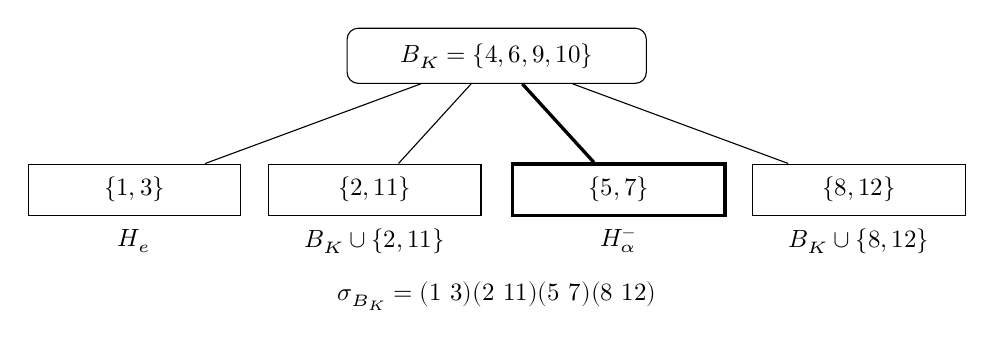
\begin{tikzpicture}[x=1cm,y=1cm, every node/.style={font=\small}]
 \node[draw,rounded corners,minimum width=3.8cm,minimum height=.7cm]
  (b) at (0,0) {$B_K=\{4,6,9,10\}$};
 \node[draw,minimum width=2.7cm,minimum height=.65cm]
  (p1) at (-4.6,-1.7) {$\{1,3\}$};
 \node[draw,minimum width=2.7cm,minimum height=.65cm]
  (p2) at (-1.55,-1.7) {$\{2,11\}$};
 \node[draw,very thick,minimum width=2.7cm,minimum height=.65cm]
  (p3) at (1.55,-1.7) {$\{5,7\}$};
 \node[draw,minimum width=2.7cm,minimum height=.65cm]
  (p4) at (4.6,-1.7) {$\{8,12\}$};
 \draw (b) -- (p1); \draw (b) -- (p2);
 \draw[very thick] (b) -- (p3); \draw (b) -- (p4);
 \node at (-4.6,-2.35) {$H_e$};
 \node at (-1.55,-2.35) {$B_K\cup\{2,11\}$};
 \node at (1.55,-2.35) {$H^-_\alpha$};
 \node at (4.6,-2.35) {$B_K\cup\{8,12\}$};
 \node at (0,-3.05)
  {$\sigma_{B_K}=(1\ 3)(2\ 11)(5\ 7)(8\ 12)$};
\end{tikzpicture}
\caption{The concrete star of the dodecaphase flag. Each line
indicates the union of the central four-element set with the pair at its endpoint; the
thick line marks the hexad also selected by the signs
preceding the carry of $\alpha$. The four pairs exhaust the eight
outer positions.}
\label{exc:fig-estrella}
\end{figure}

\begin{proposition}[The collection of stars]
\label{exc:m12}
The $\binom{12}4=495$ permutations $\sigma_B$ preserve $\mathcal H$.
The group they generate has order $95040$ and is the Mathieu group
$M_{12}$ in its action on the small Witt design.
\end{proposition}

\begin{proof}
The preservation statement reduces to the explicit definition
\eqref{exc:codigo}. Indeed, the $3^6$ words $c(w)=(w,wA)$ are traversed,
the $132$ weight-six supports are retained, and, for each
$B\in\binom{[12]}4$, the four pairs $H\setminus B$ with $B\subset H$ are
formed. These pairs partition $[12]\setminus B$; replacing each coordinate
by its mate maps the $132$ supports back onto themselves. This verification
is purely finite and proves
\(\{\sigma_B(H):H\in\mathcal H\}=\mathcal H\) for all $495$ tetrads.

To make the generation visible, six sufficient stars are written below in
cycle notation; the second column displays the tetrad fixed by each:
\[
\begin{array}{c|c|l}
i&B_i&g_i=\sigma_{B_i}\\ \hline
1&\{1,2,3,4\}&(5\ 12)(6\ 11)(7\ 9)(8\ 10)\\
2&\{1,2,3,5\}&(4\ 12)(6\ 10)(7\ 11)(8\ 9)\\
3&\{1,2,3,6\}&(4\ 11)(5\ 10)(7\ 8)(9\ 12)\\
4&\{1,2,4,5\}&(3\ 12)(6\ 9)(7\ 8)(10\ 11)\\
5&\{1,3,4,5\}&(2\ 12)(6\ 8)(7\ 10)(9\ 11)\\
6&\{2,3,4,5\}&(1\ 12)(6\ 7)(8\ 11)(9\ 10).
\end{array}
\tag{M12.1}
\label{eq:exc-seis-estrellas-m12}
\]
Let $G_i=\langle g_1,\ldots,g_i\rangle$. The finite closure can be repeated
without any implicit data through
\[
 G_i^{(0)}=\{1\},\qquad
 G_i^{(n+1)}=G_i^{(n)}\cup
 \{g_jh:1\leq j\leq i,\ h\in G_i^{(n)}\},\qquad
 G_i=\bigcup_{n\geq0}G_i^{(n)}.
\tag{M12.2}
\label{eq:exc-clausura-finita-m12}
\]
Stabilization of this recurrence gives
\[
\begin{array}{c|rrrrrr}
i&1&2&3&4&5&6\\ \hline
|G_i|&2&6&18&360&7920&95040.
\end{array}
\tag{M12.3}
\label{eq:exc-ordenes-generadores-m12}
\]
A second way to verify the last order, useful for detecting composition
errors, consists in successively fixing the points $1,2,3,4,5$. For $G=G_6$
one obtains
\[
\begin{array}{c|rrrrrr}
\text{fixed points}&0&1&2&3&4&5\\ \hline
|G_{(1,\ldots,k)}|&95040&7920&720&72&8&1\\
\text{size of the next orbit}&12&11&10&9&8&\text{---}
\end{array}
\tag{M12.4}
\label{eq:exc-cadena-estabilizadores-m12}
\]
The entries in \eqref{eq:exc-ordenes-generadores-m12} and
\eqref{eq:exc-cadena-estabilizadores-m12} are obtained solely by applying
the composition of image lists in \eqref{eq:exc-seis-estrellas-m12}; by the
orbit--stabilizer theorem, their product is
$12\cdot11\cdot10\cdot9\cdot8=95040$.

Since every $g_i$ preserves $\mathcal H$, one has
$G\leq\operatorname{Aut}(\mathcal H)$. By the uniqueness of the hexad
containing a five-element set and the incidence enumeration in
\eqref{exc:codigo}, the pointwise stabilizer of a five-element set is
trivial; consequently,
$|\operatorname{Aut}(\mathcal H)|\leq
12\cdot11\cdot10\cdot9\cdot8$. Equality of orders proves
$G=\operatorname{Aut}(\mathcal H)$; in particular, all $495$ stars belong
to $G$. The automorphism group of the resulting $S(5,6,12)$ system is, by
definition and recognition of its natural action, the Mathieu group $M_{12}$.
\end{proof}

An individual star generates a cyclic group of order two. It does
not by itself generate $M_{12}$, still less the Monster. Nor does the
existence of $495$ generators of a permutation group prove that
each is the transport of a specific TPK loop. That assertion
requires the corresponding loop map; the result established here
is the finite incidence action.

\begin{remark}[Equality of traces does not identify operators]
On $V_{11}$, a star has spectrum $+1$ with multiplicity seven
and $-1$ with multiplicity four. Its normalized trace is $3/11$.
A rank-three projector on the same space also has normalized
trace $3/11$, but spectrum $1^3,0^8$. They are not conjugate: their
minimal polynomials and spectra differ. The intertwiner
\eqref{exc:incidencia} transports defined operators; it does not turn
this scalar coincidence into an equivalence of operators.
\end{remark}

\subsection{The binary residue and the five regions of \texorpdfstring{$\pi$}{pi}}
\label{exc:cinco-regiones}

The next recognition uses the extended binary Golay code
$G_{24}$, with parameters $[24,12,8]_2$. Its weights are
$0,8,12,16,24$, and the weight-eight supports form the design
$S(5,8,24)$. Fix a dodecad $D$, the support of a weight-twelve
word. This datum and the incidence isomorphism to be declared
below belong to the realization chart; they are not used to
generate or select the decimals of $\pi$.

\begin{proposition}[Residue of a dodecad and lifting of hexads]
\label{exc:residuo-binario}
The set
\[
 \mathcal H(D)=
 \{O\cap D: O\text{ is an octad},\ |O\cap D|=6\}
\]
is an $S(5,6,12)$ system on $D$. Each of its hexads has
a unique lift to an octad. For any four-element set $B\subset D$,
the five octads containing it split into four residual
lifts and a unique octad $O_B^\perp$ with $O_B^\perp\cap D=B$.
\end{proposition}

\begin{proof}
A five-element set $A\subset D$ belongs to a unique octad $O$. If
$j=|O\cap D|$, the binary word given by the sum of $O$ and $D$ has weight
$20-2j$. Among the permitted weights, with $0\leq j\leq8$, only
$j=2,4,6$ are possible. Since $A\subset O\cap D$, we have $j\geq5$
and therefore $j=6$. This gives existence and uniqueness of the residual
hexad, as well as uniqueness of its lift by selecting five of its
points. Moreover,
\[
 \lambda_4(S(5,8,24))=\frac{\binom{20}1}{\binom41}=5,
 \qquad
 \lambda_4(S(5,6,12))=4.
\]
The four residual hexads on $B$ give four distinct octads.
The fifth cannot meet $D$ in six points, since it would be another residual
hexad; because it contains $B$, its intersection has size four and
equals $B$.
\end{proof}

A hexad-preserving chart $\ell:[12]\to D$ identifies
$\mathcal H$ with $\mathcal H(D)$. Its existence is the recognition
of the design already constructed as the small Witt design; a concrete
choice of $\ell$ fixes the relabeling. The lift
\[
 \iota_D:\mathcal H\longrightarrow
       \{\text{octads of }G_{24}\},
 \qquad H\longmapsto O\text{ such that }O\cap D=\ell(H),
\]
is injective because intersection with $D$ recovers $\ell(H)$.
The domain of this injectivity is the hexads, not the record $K$.

The relation to the five regions of $\pi$ preserves richer data
than the number five. The emissions and their signatures are:
\begin{center}
\small
\begin{tabular}{@{}crll@{}}
\toprule
Region & Multiplicity & Emission $U_6$ & Signature \\
\midrule
$\perp$ & $432$ & $(501,614,498,169,272,272)$ & $555555$ \\
$++_1$ & $144$ & $(810,923,870,169,272,272)$ & $339555$ \\
$++_2$ & $144$ & $(810,983,810,169,272,272)$ & $393555$ \\
$++_3$ & $144$ & $(870,923,810,169,272,272)$ & $933555$ \\
$--$ & $144$ & $(870,923,810,418,674,521)$ & $933717$ \\
\bottomrule
\end{tabular}
\end{center}
In each three-digit decimal block, the signature uses the modular
difference of the first two digits. The five emissions have the
same visible tritic word $w_\pi=010211$, but not the same
regional genealogy. The three positive regions preserve the tail
$169|272|272$; the negative region changes it to $418|674|521$;
the transverse region has a constant signature and greater multiplicity.

The marked extension of the regional chart sends the transverse region
to $O_{\ell(B_K)}^\perp$, the negative region to $\iota_D(H^-_\alpha)$, and the
three positive regions to the other three lifts of the star. This
realizes the $4+1$ partition of the five octads on $\ell(B_K)$.
The individual correspondence between the three positive names and
the three remaining petals requires a chart order; incidence does not
determine it without that datum. The precise claim is therefore a
marked correspondence of regions, compatible with their roles and with
the flag, not a canonical bijection inferred from the cardinality five.

The identity $432+4\cdot144=1008$ preserves the regional
multiplicities. Also, $1008=36\cdot28$, and an octad has
$\binom82=28$ pairs. These equalities are arithmetic catalog
checks, not substitutes for the map $\iota_D$ or the regional chart.

\subsubsection{Pentadic representation of the microfiber and its incidence}
\label{pi-estrella:desarrollo}

The arrangement of the five regions makes it possible to visualize
simultaneously the unity of the ternary quotient and the differentiation
preserved by the catalog. The relevant map is the restriction
\[
 \Psi\big|_{\mathscr R_\pi^{\rm micro}}:
 \mathscr R_\pi^{\rm micro}\longrightarrow\{010211\},
 \qquad \Psi(U)=(-U)\bmod3.
\]
Its five preimages are the vectors \(U_6\) in the preceding table.
Figure \ref{pi-estrella:figura} recovers their radial organization while
preserving the chart order, signatures, and multiplicities of the catalog
constructed in the preceding sections.

% Chart order and data recovered from fig_cinco_regiones_pi.tex.
\begin{figure}[H]
\centering
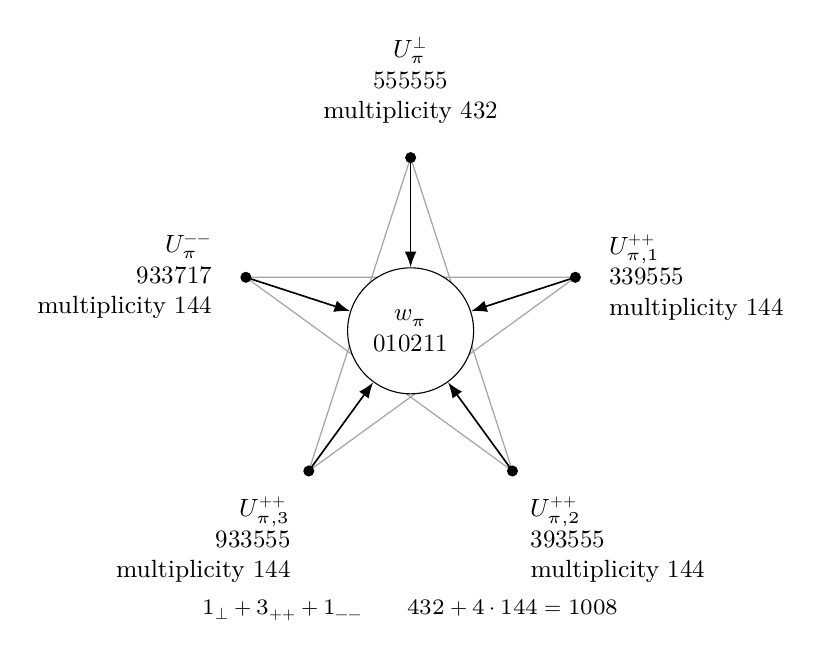
\begin{tikzpicture}[x=1cm,y=1cm,font=\small,>=Latex]
 \coordinate (a) at (90:2.2);
 \coordinate (b) at (18:2.2);
 \coordinate (c) at (-54:2.2);
 \coordinate (d) at (-126:2.2);
 \coordinate (e) at (162:2.2);
 \draw[black!35,line width=.45pt]
    (a)--(c)--(e)--(b)--(d)--cycle;
 \node[draw,fill=white,circle,minimum size=1.6cm,align=center,
    inner sep=3pt] (z) at (0,0) {$w_\pi$\\$010211$};
 \foreach \v in {a,b,c,d,e}{
    \fill (\v) circle (2pt);
    \draw[->,line width=.6pt] (\v)--(z);
 }
 \node[above=3mm,align=center] at (a)
   {$U_\pi^\perp$\\$555555$\\multiplicity $432$};
 \node[right=3mm,align=left] at (b)
   {$U_{\pi,1}^{++}$\\$339555$\\multiplicity $144$};
 \node[below right=2mm and 1mm,align=left] at (c)
   {$U_{\pi,2}^{++}$\\$393555$\\multiplicity $144$};
 \node[below left=2mm and 1mm,align=right] at (d)
   {$U_{\pi,3}^{++}$\\$933555$\\multiplicity $144$};
 \node[left=3mm,align=right] at (e)
   {$U_\pi^{--}$\\$933717$\\multiplicity $144$};
 \node[align=center,font=\footnotesize] at (0,-3.55)
   {$1_\perp+3_{++}+1_{--}$\qquad $432+4\cdot144=1008$};
\end{tikzpicture}
\caption{The five regions of \(\pi\) in a pentadic arrangement.
Each position preserves its multiplicative signature and its multiplicity;
the radial arrows represent the common projection
\(\Psi(U)=010211\). The star-shaped outline organizes the five chart
positions. Their realization in the five Witt octads is carried out through
the regional alignment and the \(4+1\) decomposition in the text.}
\label{pi-estrella:figura}
\end{figure}


Projection to the center identifies the five ternary images; the record of
the outer positions retains the regional information that makes the
incidence realization possible. The distribution
\(1_\perp+3_{++}+1_{--}\) specifies one transverse region, three positive
regions, and one negative region. Their normalized weights are \(3/7\) and
\(1/7\) for each of the remaining four: the transverse multiplicity is
threefold, even though the five images under \(\Psi\) coincide.

\Needspace{11\baselineskip}
The link with the Witt star is formulated through the already constructed
flag \(B_K\subset H^-_\alpha\), alignment \(\ell\), and lift \(\iota_D\).
The five regional positions are realized in the five octads over
\(\ell(B_K)\):
\[
\begin{aligned}
 U_\pi^\perp&\longmapsto O^\perp_{\ell(B_K)},\\
 U_\pi^{--}&\longmapsto\iota_D(H^-_\alpha),\\
 \{U_{\pi,1}^{++},U_{\pi,2}^{++},U_{\pi,3}^{++}\}
 &\longmapsto
 \{\iota_D(B_K\cup P):P\in\mathcal P_+\},\\
 \mathcal P_+&=\bigl\{\{1,3\},\{2,11\},\{8,12\}\bigr\}.
\end{aligned}
\]
The assignment of the three positive positions to the three pairs is carried
out in an ordered chart. The transverse row and the negative row are
distinguished by their regional predicates and by the flag.

The two figures are thereby articulated: Figure \ref{exc:fig-estrella} shows
the four hexads of the small Witt design over \(B_K\); Figure
\ref{pi-estrella:figura} shows the five regions that, under the alignment,
occupy the four residual octads and the transverse octad of the binary design.
The \(4+1\) law, proved in Proposition \ref{exc:residuo-binario}, specifies
the change of incidence. In this composition, \(K\) determines the marked
tetrad, and the signature of \(\alpha\) distinguishes one of its hexads. In
addition to their common ternary value, the regions preserve the structure
required for this transport to the exceptional realization.


\subsection{From the ternary code to the Niemeier lattice}
\label{exc:niemeier}

The passage to dimension twenty-four need not first go through the
binary code. It is performed directly from $C_W$ by discriminant
gluing. Two compatible prolongations thus remain distinct:
one preserves the residue $W_{12}\subset W_{24}$; the other constructs the
lattice on which the vertex operator algebra will be realized.

Let $A_2=\mathbb Z a_1\oplus\mathbb Z a_2$ with Gram matrix
\[
 \begin{pmatrix}2&-1\\-1&2\end{pmatrix},
 \qquad \rho=a_1+a_2,\qquad \rho^2=2.
\]
Represent the three classes of $A_2^*/A_2$ by
\[
 \varpi_0=0,\qquad
 \varpi_1=\frac{2a_1+a_2}{3},\qquad
 \varpi_2=\frac{a_1+2a_2}{3}.
\]
The map $j\mapsto\varpi_j+A_2$ additively identifies
$\mathbb F_3$ with this discriminant. For $c\in C_W$, write
$\phi(c)=(\varpi_{c_1},\ldots,\varpi_{c_{12}})$ and define
\begin{equation}
 N(C_W)=\bigcup_{c\in C_W}\bigl(A_2^{12}+\phi(c)\bigr).
 \label{exc:niemeier-def}
\end{equation}

\begin{theorem}[Ternary gluing]
\label{exc:niemeier-teorema}
The object \eqref{exc:niemeier-def} is a positive, even,
unimodular lattice of rank $24$. Its root system is exactly
$A_2^{12}$; it is therefore recognized as the Niemeier lattice with
that root system.
\end{theorem}

\begin{proof}
Linearity of the code makes the union of classes stable under
addition. Self-orthogonality annihilates the discriminant pairing:
the latter is a multiple of $c\cdot d/3$ modulo $\mathbb Z$. Thus the
lattice is integral. The norm of a glue class is
$2\operatorname{wt}(c)/3$ modulo $2\mathbb Z$. The weights in
\eqref{exc:enumerador} are multiples of three, so the lattice is even.

The index of $A_2^{12}$ in $N(C_W)$ is $|C_W|=3^6$. Consequently,
\[
 \det N(C_W)=\frac{3^{12}}{(3^6)^2}=1.
\]
Positivity follows from the orthogonal sum of the twelve $A_2$ metrics.
In a nonzero class of $A_2^*/A_2$, the minimum norm is $2/3$;
every nonzero word has at least six nonzero positions.
Hence a vector in a nontrivial glue class has norm
at least $6\cdot2/3=4$. No norm-two roots occur outside
$A_2^{12}$. Within it, the roots are precisely those of its
twelve components.
\end{proof}

\subsection{Incidence selection of the rootless unimodular neighbor}
\label{exc:leech}

\paragraph{From the incidence origin to the lattice modification.}
\label{inc-ampl-reticulo}
The marked flag determines a position through an equivariant set-theoretic
operation:
\[
 o_*=(H_e\cap H_\varphi)
       \setminus(H^-_\alpha\cup H_{\rm APP})=\{1\}.
\]
Its role is to distinguish one component among the twelve involved in the
lattice realization. The complete ternary code acts as a gluing code in the
discriminant module $(A_2^*/A_2)^{12}$. Its preimage defines $N(C_W)$, and
the self-duality, weights, and distance of the code translate, respectively,
into integrality and determinant properties, parity, and norm bounds for the
gluing classes. Here the symbolic information of the code performs a role
that the isolated support no longer performs.

The $A_2$ metric and the positive radial chamber are fixed in the lattice
construction. Within that chamber, the congruence required for an even
neighbor of index three has twelve realizations of minimum norm $54$,
permuted by changing the distinguished component. The origin $o_*$ selects
\[
 v_\alpha=4\rho_1+\rho_2+\cdots+\rho_{12},\qquad
 v_\alpha^2=2(4^2+11)=54.
\]
The coefficient $4$ belongs to that solution of the congruence in the
declared chamber. The subscript $\alpha$ records the incidence provenance of
the selection: its content is the frame that entered the closure and now
individuates a lattice direction.

Pairing with $v_\alpha$ determines the index-three sublattice
$N_{\alpha,0}$, and adjoining the class $v_\alpha/3$ produces the neighbor
$N_\alpha$ in \eqref{exc:vecino}. This modification preserves the rank and
recovers unimodularity and parity; selection by congruence eliminates the
previous roots, and the local bounds exclude roots in the new classes.
Identification with the Leech lattice occurs after these verifications. The
binary realization of the five regions and this lattice construction are two
prolongations of the common frame: the latter directly receives the ternary
code as gluing data.


The label $o_*=1$ of the flag is now realized as one of the
twelve $A_2$ components. This operation declares the preceding metric and
the positive radial chamber
\[
 v(a)=\sum_{i=1}^{12}a_i\rho_i,
 \qquad a_i=1+3b_i,\quad b_i\in\mathbb Z_{\geq0}.
\]
The evenness requirement for the index-three neighbor is
$v(a)^2\equiv0\pmod{18}$. Since
\[
 v(a)^2=2\sum_i(1+3b_i)^2,
\]
this congruence is equivalent to $\sum_i b_i\equiv1\pmod3$. The least
norm in the chamber is obtained with a single $b_i=1$ and
all others zero; it is $54$. The marked origin selects
\begin{equation}
 v_\alpha=4\rho_1+\rho_2+\cdots+\rho_{12},
 \qquad v_\alpha^2=54.
 \label{exc:vector}
\end{equation}
The word ``least'' refers to this positive chamber. It does not assert
minimality throughout the residual class: the vector
$(a_1-2a_2,\rho,\ldots,\rho)$ represents the same class modulo three
and has norm $14+11\cdot2=36$. The chamber restriction is part
of the construction data, not an omissible conclusion.

Let $N=N(C_W)$. Define
\begin{equation}
 N_{\alpha,0}=\{x\in N:\langle x,v_\alpha\rangle\equiv0\pmod3\},
 \qquad
 N_\alpha=N_{\alpha,0}+\mathbb Z\frac{v_\alpha}{3}.
 \label{exc:vecino}
\end{equation}

\begin{theorem}[Leech neighbor determined by the marked flag]
\label{exc:teorema-leech}
With the declared metric and chamber, $N_\alpha$ is a positive, even,
unimodular lattice of rank $24$, with no vectors of norm two.
By the corresponding classification theorem, it is isometric to the
Leech lattice $\Lambda_{24}$.
\end{theorem}

\begin{proof}
The character $x\mapsto\langle x,v_\alpha\rangle\bmod3$ is nonzero:
a simple root of a component pairs with $a_i\rho_i$ to give
$a_i\equiv1\pmod3$. Hence $[N:N_{\alpha,0}]=3$ and
$\det N_{\alpha,0}=9$. Moreover,
$v_\alpha/3\in N_{\alpha,0}^*$ and $v_\alpha\in N_{\alpha,0}$.
If $v_\alpha/3$ belonged to $N$, the integrality of $N$ would make
all pairings with $v_\alpha$ divisible by three,
contradicting the nonzero character. The class of $v_\alpha/3$ therefore
has order three. It follows that
\[
 [N_\alpha:N_{\alpha,0}]=3,
 \qquad \det N_\alpha=9/3^2=1.
\]
The extension is integral, and for $x\in N_{\alpha,0}$,
\[
 \left(x+m\frac{v_\alpha}{3}\right)^2
   =x^2+2m\frac{\langle x,v_\alpha\rangle}{3}+6m^2
   \in2\mathbb Z.
\]
Hence it is even.

It remains to exclude roots, the decisive step. The roots of $N$
belong to $A_2^{12}$. Their pairings with $v_\alpha$ are
congruent to $\pm1$ or $\pm2$ modulo three; none belongs to
$N_{\alpha,0}$. For the other two classes of the neighbor, each component
belongs to one of the local classes
\[
 A_2+\varpi_j\pm\rho/3,\qquad j=0,1,2.
\]
Since $4\rho/3\equiv\rho/3\pmod{A_2}$, this description also holds
in the distinguished component. Writing a local vector
as $(u a_1+v a_2)/3$, its norm is
$2(u^2-uv+v^2)/9$. The six preceding classes have nonzero residues
and minimum $2/9$: representatives minimizing the quadratic form
are $(\pm1,0),(0,\pm1),(1,1),(-1,-1)$ in the appropriate residues.
A vector in a new class therefore has norm at least
$12\cdot2/9=8/3>2$. There are no roots in any of the three classes.
The classification of positive even unimodular lattices of
rank twenty-four identifies the unique rootless case with
$\Lambda_{24}$.
\end{proof}

The argument does not recognize Leech from a coincidence of dimension.
It constructs the gluing, proves integrality, evenness, and the determinant, and
eliminates roots through a local bound. Only then does it apply the
classification theorem. The dependence on $\alpha$ is preserved in
the flag selecting $o_*$ and in the vector \eqref{exc:vector};
the scalar value of the constant is not converted into a length of the
lattice.

\subsection{The vertex operator algebra and the Monster}
\label{exc:voa}

Let $\Lambda=N_\alpha$, already recognized as Leech. The next step
uses its integral lattice, not a decimal expansion. The lattice
vertex operator algebra construction is written
\[
 V_\Lambda=M(1)\otimes\mathbb C_\varepsilon[\Lambda].
\]
Here $M(1)$ is the rank-twenty-four Heisenberg oscillator
space; $\mathbb C_\varepsilon[\Lambda]$ is the group algebra
twisted by the cocycle of the central extension of the lattice. The
cocycle and the lift of the isometries are part of the
construction: a bare vector-space sum does not determine the vertex
products.

Negation $\lambda\mapsto-\lambda$ admits the standard lift
$\theta$. With its twisted module and the compatible parity choice,
the Frenkel--Lepowsky--Meurman construction produces
\begin{equation}
 V^\natural_{\rm HMT}
   =V_\Lambda^+\oplus(V_\Lambda^T)^+.
 \label{exc:flm}
\end{equation}
The sign $+$ denotes the even part of the lifted action. The expression
includes the orbifold vertex product; it is not merely a sum
of graded spaces.

\begin{theorem}[Prolongation to the Moonshine module]
\label{exc:moonshine}
The algebra \eqref{exc:flm}, constructed on the neighbor
\eqref{exc:vecino}, is a realization of the Moonshine algebra
$V^\natural$. It has central charge $24$, a zero weight-one component,
and an automorphism group isomorphic to the Monster $\mathbb M$. Its graded
character is
\begin{equation}
 \operatorname{Tr}_{V^\natural_{\rm HMT}}q^{L_0-1}
   =J(\tau)=j(\tau)-744
   =q^{-1}+196884q+21493760q^2+\cdots,
 \qquad q=e^{2\pi i\tau}.
 \label{exc:j}
\end{equation}
\end{theorem}

\begin{proof}
Theorem \ref{exc:teorema-leech} verifies the lattice hypotheses:
positivity, evenness, unimodularity, rank twenty-four, and absence of
roots. The Frenkel--Lepowsky--Meurman construction and theorem
for the Leech lattice then apply. They identify
the orbifold with $V^\natural$ and establish its character and its
automorphisms. The composition of the flag, the neighbor, and the vertex
operator algebra (VOA) construction functor gives the realization indicated
here. It is not deduced from the coefficient $196884$.
\end{proof}

The theorem used is a subsequent classical recognition with verified
hypotheses, not a new proof in this article of the
Frenkel--Lepowsky--Meurman (FLM) construction \cite{flm}.
Moreover, the notation $q=e^{2\pi i\tau}$ is the conventional Fourier
variable used to recognize the character. It does not introduce $\pi$
or $e$ as inputs into the coinductive generator that has already determined them.

Part of the trace mechanism can be seen before the orbifold.
Only the zero lattice vector is fixed by negation; each
oscillator contributes an alternating sign. Hence
\[
 \operatorname{Tr}_{V_\Lambda}\theta q^{L_0-1}
   =t_2(\tau)
   :=q^{-1}\prod_{n\geq1}(1+q^n)^{-24}.
\]
This trace in the lattice algebra must not be confused with the
character of $V^\natural$ without insertion. Nor does it by
itself identify a Monster conjugacy class: the space, insertion,
and lift must be specified before functions are compared.

\paragraph{Grading, unit, and automorphisms.}
\label{inc-ampl-automorfismos}
The Frenkel--Lepowsky--Meurman construction is applied to the lattice
$N_\alpha$ once its properties have been verified. It incorporates the
oscillator space, the central extension of the lattice, the vertex product,
and the sector twisted by the lift of negation. The result is the algebra
$V^\natural_{\rm HMT}$ in \eqref{exc:flm}, whose automorphism group is
isomorphic to the Monster. Its domain of action is thus fixed by an
algebraic structure with a grading and a product. Borcherds's Moonshine
theorem subsequently determines the graded traces with insertion of those
automorphisms \cite{flm,borcherds}.

At this level the unit acquires a precise realization: the weight-zero
component is the vacuum line and contributes the coefficient $1$ of $q^{-1}$
in the graded character. At the cylinder level, the refinement maps preserve
the constant function by precomposition. Each preservation statement
therefore has its own object and map. The development of the proofs makes
this continuity of construction visible, from the arithmetic operations and
memory through incidence, the metric, and the vertex products.

This articulation places $K$ and the closure of $\alpha$ within the main
argument. $K$ reversibly preserves an integral coordinate of the history;
the normalization of $\alpha$ composes the regional records with that
coordinate; the signed configuration determines a flag; and the marked flag
selects the lattice modification on which Moonshine is realized. The proofs
that follow develop these maps, distinguishing reversible equivalences,
information quotients, and realizations that add a metric or algebraic
structure. A provable relation among structure, equation, and value is thus
expressed while preserving the attribution of each construction and the scope
of its theorems.


\subsection{Ternary orientation of the Leech neighbor}
\label{km:orden-tres-reticular}

The order-two presentation constructed above uses negation
of the Leech lattice. The same lattice, obtained from the incidence marked
by \(K\) and the dodecaphase support of \(\alpha\), admits a second
presentation compatible with the ternary character of the construction.
To make this continuity explicit, the gluing is retained, its order-three
isometry is constructed, and preservation of the already selected neighbor
is verified. This step requires no alteration of \(K\), its rational reading,
or the preceding definition of \(\alpha\). The lattice operations and the
hypotheses of the recognition theorems used are specified below.

We work in the basis of simple roots of each \(A_2\) factor, with
\begin{equation}
 B_2=\begin{pmatrix}2&-1\\-1&2\end{pmatrix},\qquad
 \mathsf C=\begin{pmatrix}0&-1\\1&-1\end{pmatrix},\qquad
 \mathsf R=\begin{pmatrix}0&1\\1&0\end{pmatrix},\qquad
 \rho=\begin{pmatrix}1\\1\end{pmatrix}.
 \label{km:coxeter-reflexion}
\end{equation}
Multiplication gives
\[
 \mathsf C^3=I_2,\quad
 \mathsf C^2+\mathsf C+I_2=0,\quad
 \mathsf C^{\mathsf T}B_2\mathsf C=B_2,\quad
 \mathsf R\mathsf C\mathsf R=\mathsf C^{-1},\quad
 \mathsf R^{\mathsf T}B_2\mathsf R=B_2.
\]
These identities fix both the metric and the orientation of the action.
In the discriminant \(A_2^*/A_2\cong\mathbb F_3\), we take
the class of \(\varpi=(2,1)^{\mathsf T}/3\) as generator. We have
\(\mathsf C\varpi-\varpi=(-1,0)^{\mathsf T}\), so
\(\mathsf C\) acts trivially on the discriminant; the reflection
\(\mathsf R\) reverses its sign.

The Paley--Witt matrix already constructed produces a full-support
element by the following operation:
\begin{equation}
 \begin{gathered}
 q_*=(1,1,1,1,1,1),\qquad q_*A_W=(2,1,1,1,1,1),\\
 c_*=(q_*,q_*A_W)
 =(1,1,1,1,1,1,2,1,1,1,1,1)\in C_W.
 \end{gathered}
 \label{km:palabra-total}
\end{equation}
Every coordinate of \(c_*\) is nonzero. For the twelve positions,
define the frames and the isometry
\begin{equation}
 P_b(c_*)=
 \begin{cases}\mathsf R,&(c_*)_b=1,\\I_2,&(c_*)_b=2,\end{cases}
 \qquad
 g_c=\bigoplus_{b=1}^{12}P_b(c_*)\mathsf C P_b(c_*)^{-1}.
 \label{km:isometria-ternaria}
\end{equation}
The symbol \(P_b(c_*)\) here denotes an invertible frame of an
\(A_2\) factor, not the three-dimensional isotypic projector \(P_3\).

\begin{proposition}[Order-three isometry on the marked neighbor]
\label{km:estabilidad-vecino}
The operator \(g_c\) is an order-three isometry with no nonzero
fixed vectors. It preserves the Niemeier lattice \(N=N(C_W)\) and the
neighbor \(N_\alpha\) constructed in \eqref{exc:vecino}.
\end{proposition}
\begin{proof}
Each block of \(g_c\) is \(\mathsf C\) or \(\mathsf C^{-1}\);
its minimal polynomial is \(X^2+X+1\). This proves its order and
the absence of fixed vectors. Both blocks act trivially on the
discriminant, so they preserve every gluing class and therefore
the lattice \(N\).

Write \(v=v_\alpha=4\rho_{o_*}+\sum_{b\ne o_*}\rho_b\),
with the frames and incidence origin already fixed. Its radial
coefficients are \(a_{o_*}=4\) and \(a_b=1\) for \(b\ne o_*\).
All satisfy \(a_b\equiv1\pmod3\). In one factor,
\[
 (\mathsf C-I_2)\rho=(-2,-1)^{\mathsf T},\qquad
 (\mathsf C^{-1}-I_2)\rho=(-1,-2)^{\mathsf T}.
\]
After division by three, their discriminant classes are
\(2\) and \(1\), respectively. Consequently, the vectors
\begin{equation}
 y=\frac{g_cv-v}{3},\qquad z=\frac{g_c^{-1}v-v}{3}
 \label{km:desplazamientos}
\end{equation}
have discriminant words \(c_*\) and \(-c_*\), both in
\(C_W\). Hence \(y,z\in N\). The local product is
\[
 \left\langle
 \frac{(\mathsf C^{\pm1}-I_2)a_b\rho}{3},a_b\rho
 \right\rangle=-a_b^2,
\]
and summing gives
\(\langle y,v\rangle=\langle z,v\rangle=-(16+11)=-27\).
Thus, \(y,z\in N_0=\{x\in N:\langle x,v\rangle\equiv0\pmod3\}\).
For \(x\in N_0\),
\[
 \langle g_cx,v\rangle
 =\langle x,g_c^{-1}v\rangle
 =\langle x,v\rangle+3\langle x,z\rangle\equiv0\pmod3.
\]
The argument applied to \(g_c^{-1}\) proves \(g_cN_0=N_0\).
Finally, \(g_c(v/3)=v/3+y\) preserves the class generating
\(N_\alpha=N_0+\mathbb Z(v/3)\). We obtain
\(g_cN_\alpha=N_\alpha\).
\end{proof}

The proof preserves more than the lattice dimension: it uses the
gluing code, its orientation, the flag origin, and the congruence of the
radial vector. These data explain why the second presentation
remains linked to the dodecaphase register from which the construction began.

\subsection{Ternary trace, twisted weight, and order-three extension}
\label{km:orbifold-tres}

Let \(\Lambda=N_\alpha\), and let \(\widehat g_c\) be the standard
lift of \(g_c\) to the lattice algebra
\(V_\Lambda=M(1)\otimes\mathbb C_\varepsilon[\Lambda]\), with the
central extension and cocycle already specified. The odd order allows
this lift to be chosen of order three. Each complex \(A_2\) factor
contributes the eigenvalues \(\zeta_3\) and \(\zeta_3^2\), where
\(\zeta_3^2+\zeta_3+1=0\).

\begin{proposition}[Graded trace and type of the lift]
\label{km:traza-tipo}
For \(j=1,2\),
\begin{equation}
 \operatorname{Tr}_{V_\Lambda}
       \bigl(\widehat g_c^{\,j}q^{L_0-1}\bigr)
 =t_3(\tau)
 :=q^{-1}\prod_{n\ge1}(1+q^n+q^{2n})^{-12}.
 \label{km:tres-traza}
\end{equation}
The lowest weight of the nontrivial twisted modules is \(4/3\), and
the lift is of type zero.
\end{proposition}
\begin{proof}
Only the zero vector contributes to the lattice part of the trace,
because \(g_c\) and \(g_c^2\) have no nonzero fixed vectors.
At each oscillator degree, the trace of symmetric powers is the inverse
of the determinant \(I-g_c^jq^n\). Each \(A_2\) factor contributes
\(1+q^n+q^{2n}\), proving \eqref{km:tres-traza}.

The twisted-vacuum weight formula for an order-three lattice
automorphism, applied to the two twelve-dimensional eigenspaces, gives
\[
 \rho_{\widehat g_c}
 =\frac{1}{4\cdot3^2}
   \bigl(1\cdot2\cdot12+2\cdot1\cdot12\bigr)=\frac43.
\]
The type is the class of \(3^2\rho_{\widehat g_c}=12\) modulo
three, which is zero. The weight formula is a result of twisted-module
theory; the multiplicities and isometry supplied to it
have been constructed here.
\end{proof}

\begin{theorem}[Second presentation of the Moonshine algebra]
\label{km:moonshine-tres}
The type-zero cyclic extension
\begin{equation}
 V_{(3)}=\operatorname{Orb}_{\mathbb Z/3}
                 (V_\Lambda,\widehat g_c)
 \label{km:extension-orden3}
\end{equation}
is isomorphic to the vertex operator algebra \(V^\natural\).
\end{theorem}
\begin{proof}
Theorem \ref{exc:teorema-leech} provides a positive,
even, unimodular, rootless lattice of rank twenty-four.
Proposition~\ref{km:estabilidad-vecino} constructs an order-three
fixed-point-free isometry on that same lattice;
Proposition~\ref{km:traza-tipo} verifies the lift and its type.
The Chen--Lam--Shimakura theorem on the order-three orbifold
of the Leech lattice algebra then applies
\cite[Theorem~1.1]{chenlamshimakura2016}. This identification is also covered
by the uniform treatment of Abe--Lam--Yamada
\cite[Theorem~4.4 and Sections~2--4]{abelamyamada2017}. This application follows construction
of the lattice data; equality of characters does not replace the
hypotheses of the theorem used.
\end{proof}

To specify the dual symmetry, write
\(V_{(3)}=W_0\oplus W_1\oplus W_2\), where \(W_i\) is the
integral sector selected in the \(\widehat g_c^{\,i}\)-twisted module.
The product satisfies
\(Y(W_i,z)W_j\subset W_{i+j\bmod3}((z))\). Hence
\begin{equation}
 g^\vee|_{W_i}=\zeta_3^i I
 \label{km:dual-ciclico}
\end{equation}
defines an order-three automorphism. Indeed, the factor on a
product is \(\zeta_3^{i+j}=\zeta_3^i\zeta_3^j\), and the vacuum and
conformal vector belong to \(W_0\). The classical identification of
this automorphism in the Monster is class \(3B\), with series
\(T_{3B}=t_3+12\) \cite{kmconwaynorton1979,borcherds}.
This normalization can be checked in the construction. The lattice
character is \(\operatorname{ch}V_\Lambda=J+24\): its initial pole
is \(q^{-1}\), its weight-one space has dimension 24, and the
weight-zero modular character is determined by these data.
If \(F\) is the character of the fixed subspace and \(H\) that of each
integral twisted sector, projection onto invariants and conjugation
of the two sectors give
\[
 F=\frac{J+24+2t_3}{3},\qquad F+2H=J,
 \qquad \operatorname{Tr}g^\vee q^{L_0-1}=F-H=t_3+12.
\]
Its domain is the extended algebra, whereas
\(\widehat g_c\) acts on the preceding lattice algebra.

\subsection{Equivalence of the order-two and order-three presentations}
\label{km:equivalencia-dos-tres}

Denote by
\[
 V_{(2)}=(V_\Lambda)^+\oplus(V_\Lambda^T)^+
\]
the FLM presentation in \eqref{exc:flm}. Both presentations preserve
the same Leech neighbor as their antecedent. Their extensions employ
different automorphisms and vertex products determined by
the respective lifting data.

\begin{theorem}[Graded equivalence and transport of automorphisms]
\label{km:equivalencia-voa}
Given vertex operator algebra isomorphisms
\[
 \phi_2:V_{(2)}\xrightarrow{\ \cong\ }V^\natural,
 \qquad
 \phi_3:V_{(3)}\xrightarrow{\ \cong\ }V^\natural,
\]
the composition
\begin{equation}
 \Phi_{23}=\phi_2^{-1}\phi_3:
 V_{(3)}\xrightarrow{\ \cong\ }V_{(2)}
 \label{km:Phi23}
\end{equation}
preserves the vacuum, conformal vector, grading, and vertex
product. Conjugation by \(\Phi_{23}\) identifies the automorphism
groups and preserves their graded traces.
\end{theorem}
\begin{proof}
The composition of the two isomorphisms preserves the stated
structures. In particular,
\[
 \Phi_{23}Y_{(3)}(a,z)b
 =Y_{(2)}(\Phi_{23}a,z)\Phi_{23}b,
 \qquad
 \Phi_{23}L_0^{(3)}=L_0^{(2)}\Phi_{23}.
\]
If \(h\) is an automorphism of \(V_{(3)}\), then
\(h' =\Phi_{23}h\Phi_{23}^{-1}\) is an automorphism of
\(V_{(2)}\). Equality of traces on each finite-dimensional homogeneous
component gives
\[
 \operatorname{Tr}_{V_{(3)}}h q^{L_0-1}
 =\operatorname{Tr}_{V_{(2)}}h' q^{L_0-1}.
\]
\end{proof}

The choice of \(\phi_2\) and \(\phi_3\) forms part of the statement;
\(\Phi_{23}\) is not presented as a canonical identification
independent of these choices. Nor does it transform an order-three
automorphism into the order-two involution: conjugation preserves
order. Its content is that two different extensions realize the
same graded structure, with explicit transport of their products,
representations, and traces.

\subsection{Eta functions, Fricke involution, and vacuum normalization}
\label{km:fricke}

For \(\operatorname{Im}\tau>0\), the traces of the two lattice
automorphisms admit the expressions
\begin{equation}
 \eta(\tau)=q^{1/24}\prod_{n\ge1}(1-q^n),\qquad
 t_2=\left(\frac{\eta(\tau)}{\eta(2\tau)}\right)^{24},\qquad
 t_3=\left(\frac{\eta(\tau)}{\eta(3\tau)}\right)^{12}.
 \label{km:eta-trazas}
\end{equation}
They follow directly from the factorizations
\(1-q^{2n}=(1-q^n)(1+q^n)\) and
\(1-q^{3n}=(1-q^n)(1+q^n+q^{2n})\). The order in \(q\) of the
level-three quotient, before raising it to the twelfth power, is
\[
 \frac1{24}-\frac3{24}=-\frac1{12};
 \qquad 12\left(-\frac1{12}\right)=-1.
\]
Here \(-1/12\) denotes the exact difference between the initial
exponents of two eta functions. The operation is specified and
does not require interpreting a divergent sum as a convergent one.
Agreement with other normalized defects in the corpus preserves
their respective realizations; it does not identify their operators
through equality of the scalar.

\begin{proposition}[Fricke involution on the order-two trace]
\label{km:fricke-prop}
Let \(w_2\tau=-1/(2\tau)\). Then
\begin{equation}
 t_2(w_2\tau)=\frac{2^{12}}{t_2(\tau)},\qquad
 T_{2A}=t_2+24+\frac{2^{12}}{t_2}
 \label{km:fricke-t2}
\end{equation}
and \(T_{2A}(w_2\tau)=T_{2A}(\tau)\).
\end{proposition}
\begin{proof}
The transformation law
\(\eta(-1/\tau)=(-i\tau)^{1/2}\eta(\tau)\) gives
\[
 \frac{\eta(-1/(2\tau))}{\eta(-1/\tau)}
 =\sqrt2\,\frac{\eta(2\tau)}{\eta(\tau)}.
\]
The twenty-fourth power yields the first identity. Substitution
interchanges the two variable terms of \(T_{2A}\) and fixes
the constant term. Recognition of this expression as the
McKay--Thompson series of class \(2A\) corresponds to the
level-two symmetrization of Conway--Norton
\cite[\S\S4 and 6, Table~3]{kmconwaynorton1979} and the
Moonshine theorem \cite{borcherds}.
\end{proof}

The modular uniformizations of levels two and three, with the
preceding normalizations, are
\begin{align}
 j&=\frac{(t_2+256)^3}{t_2^2},
 \label{km:j-nivel2}\\
 J=j-744
 &=t_3+12+\frac{10\cdot3^9}{t_3}
       +\frac{4\cdot3^{14}}{t_3^2}
       +\frac{3^{18}}{t_3^3}.
 \label{km:j-nivel3}
\end{align}
They are used as classical modular identities on the traces already
constructed, not as rules for selecting the code or the neighbor.
The second can also be written
\(j=(t_3+27)(t_3+243)^3/t_3^3\).
The direct product expansion of \eqref{km:tres-traza} begins with
\[
 t_3=q^{-1}-12+54q-76q^2-243q^3+1188q^4+O(q^5).
\]
In particular, \([q]J=54+10\cdot3^9=196884\); this is a
consequence of the traces and uniformization. The construction of
\(V^\natural\) retains its lattice and orbifold proof,
independently of this check of the first coefficient.

The three operations occurring in this extension have
different domains. The dual symmetry \(g^\vee\) acts on sectors
of the vertex algebra; Fricke acts on the modular parameter and
its function; radius duality interchanges momentum and winding
in the compact lattice sector. Their reciprocity formulas can
be coordinated through the corresponding maps, but the name
“duality” does not replace those maps. This distinction allows the
construction to continue toward dimensional screens while preserving
incidence, grading, and the origin of each operation.

% NEW BIBITEMS: copy into the article's thebibliography environment.
% Primary verification: arXiv 1606.05961v2 (Theorem 1.1);
% arXiv 1705.09022v4 (Sections 2--4);
% Conway--Norton, pp. 311 and 314--315, Table 3.
% \bibitem{chenlamshimakura2016}
% H.-Y. Chen, C. H. Lam and H. Shimakura,
% ``$\mathbb Z_3$-orbifold construction of the Moonshine vertex operator
% algebra and some maximal $3$-local subgroups of the Monster'',
% preprint, arXiv:1606.05961 (2016), version 2 (2017).
% \href{https://arxiv.org/abs/1606.05961}{arXiv:1606.05961}.
% \bibitem{abelamyamada2017}
% T. Abe, C. H. Lam and H. Yamada,
% ``A remark on $\mathbb Z_p$-orbifold constructions of the Moonshine
% vertex operator algebra'', preprint, arXiv:1705.09022 (2017).
% \href{https://arxiv.org/abs/1705.09022}{arXiv:1705.09022}.
% \bibitem{kmconwaynorton1979}
% J. H. Conway and S. P. Norton, ``Monstrous Moonshine'',
% \emph{Bulletin of the London Mathematical Society} \textbf{11},
% 308--339 (1979).
% \href{https://doi.org/10.1112/blms/11.3.308}{doi:10.1112/blms/11.3.308}.


% REV02: proofs consolidated in 02_dualidad_t.tex and 03_pantallas_coordinadas.tex.
\subsection{Exceptional incidence and coordination of the screens}
\label{exc:pantallas-dualidad}

The direction selected by \(K\) and the Leech lattice arise from distinct
representations of the constructed incidence. The former determines the
orthogonal reduction \(12\to11\to10\); the latter enters the isotropic
reduction \(26\to24\). The coordination preserves the preceding space, its
relations, and the information transmitted by each projection.

The sectoral representation on T-duality and dimensional screens jointly
develops this coordination. Its first block brings together the involution of
integer coordinates, unitary conjugation with its domains, and the change of
residual section with quotient memory. The second constructs the morphism
\(\mathcal R_M^{\mathrm{alg}}\) and proves the isomorphism of the quotient
presentations. The graph preserves the coordinate in \(V_{11}\) together
with its projection onto \(V_{10}\), while the isotropic quotient recovers
the Leech lattice. The respective kernels and codomains are thus preserved.

The action ellipse is constructed before duality is applied and fixes its
dimensionless radius together with the reciprocal radius. The compact sector
then links exceptional incidence to a determined quadratic form. The fields,
action, and operators of the subsequent physical realization are presented
in their proper domain, preserving this algebraic antecedent and its internal
proofs.


\subsection{Graded Moonshine traces and representation of the Monster}
\label{exc:alcance}

For $g\in\operatorname{Aut}(V^\natural_{\rm HMT})$, the trace
with insertion is
\[
 T_g(\tau)=
 \operatorname{Tr}_{V^\natural_{\rm HMT}}gq^{L_0-1}.
\]
The monstrous Moonshine theorem identifies these series as
Hauptmoduln of the corresponding genus-zero groups
\cite[Theorem~1.1]{borcherds}.
The character $J$, the group $\mathbb M$, and the collection $g\mapsto T_g$
are realizations of the algebra already constructed. They do not form a causal
sequence in which one first guesses $J$ and then infers the Monster.

The unit has a precise algebraic location here. The weight-zero
subspace is the vacuum line, \(V^\natural_0=\CC\mathbf1\), and
the coefficient of \(q^{-1}\) in \(J\) is therefore \(1\). In weight one
the dimension is zero, accounting for the absence of the constant term
in \(J=j-744\). A morphism of vertex algebras preserves the vacuum
vector. This property provides the technical meaning of preservation
of the unit at this level; the unit of cylindrical observables
is preserved by the precomposition proved earlier. The relation
between the two levels must follow the construction maps with their units.

In weight two, the equality
\[
 196884=1+196883=196560+324=54(5\cdot729+1).
\]
appears. The first decomposition corresponds to the trivial conformal line and the
irreducible component of dimension $196883$ in the Monster
representation. The other expressions have lattice-theoretic or
arithmetic readings. Their equality does not automatically identify their summands
with TPK regions, words, or routes. Doing so would require
presenting the maps between those spaces and proving that they respect the
relevant actions.

In particular, an isometry $N_\alpha\simeq\Lambda_{24}$ induces
a realization of \eqref{exc:flm}, and a choice of isomorphism
with $V^\natural$ transports its automorphism group. This does not
construct an action of the Monster on the digits of
$\pi$, on the blocks of $K$, or on all TPK histories.
Such an additional assertion would require a representation
$\rho_{\rm TPK}$ and a map $F$ with an explicit square
\[
 F\rho_{\rm TPK}(g)=\rho_{V^\natural}(g)F,
\]
including domain, codomain, and preserved information. The absence
of that step from the present claim does not remove the incidence
intertwiner $U_W$, the flag, or the neighbor already constructed; it only
delimits a different promotion, namely an action on the source state.

The chain established in this section can be summarized, keeping
its transport data visible, as
\begin{align*}
 &\text{APP--TRIT--TPK and arithmetic state with trajectory memory}
   \longrightarrow (w_j,f_j;K,Z_0)\\
 &\longrightarrow (C_W,\mathcal H;B_K\subset H^-_\alpha,
                   P_\pi,H_e,H_\varphi,H_{\rm APP})\\
 &\longrightarrow \bigl(N(C_W),o_*,\text{metric and chamber}\bigr)
   \longrightarrow N_\alpha
   \longrightarrow V^\natural_{\rm HMT}.
\end{align*}
At the incidence level, the stars generate $M_{12}$, and the
residual chart realizes the regional $4+1$ structure in $W_{24}$.
At the lattice and VOA level, the construction gives Leech and the
Moonshine module. These are prolongations of the same marked source, with
different objects and maps. Causal continuity does not require
identifying their codomains or erasing the explicit choices
of frame, chamber, and lift.

The result of this section is therefore an assembled derivation:
the finite and lattice proofs make the passage from dodecaphase incidence
to the hypotheses of the recognition theorems effective. Every arrow used is
defined in the development, and its conclusion is obtained within the stated
domains. Experimental identification of physical realizations remains
separate from this internal proof and from the subsequent comparison of
constants.


\clearpage
\section{Conclusions: affirmative resolution of the Continuum Hypothesis}
\label{sec:conclusiones-ch}
\begingroup
\fontsize{10.5}{13.4}\selectfont
\setlength{\parskip}{3pt}
\setlength{\abovedisplayskip}{5pt}
\setlength{\belowdisplayskip}{5pt}

The main result is the absence of intermediate cardinals between the natural
numbers and the real line within the HMT genealogical closure. For each
realized history, the construction of that closure and the two cardinal
injections establish
\begin{equation}
 \boxed{
 \mathfrak G_{\mathrm{HMT}}(h,m_\infty)
 \models 2^{\aleph_0}=\aleph_1 .}
 \label{eq:conclusion-decision-continuo}
\end{equation}
The equality is not presupposed at any generative stage. Exhaustive cylinder
coverage establishes the equinumerosity
\[
 \mathbb R_{\mathrm{HMT}}^{\mathfrak G}
 \approx\mathcal P^{\mathfrak G}(\omega).
\]
Genealogical condensation assigns to every internal real an ordinal strictly
below \(\omega_1^{\mathfrak G}\) and constructs
\[
 j_{\mathrm{HMT}}:
 \mathbb R_{\mathrm{HMT}}^{\mathfrak G}\hookrightarrow
 \omega_1^{\mathfrak G}.
\]
The coding of countable well-orders and its ternary lift construct the
injection in the opposite direction
\[
 k_{\mathrm{HMT}}:
 \omega_1^{\mathfrak G}\hookrightarrow
 \mathbb R_{\mathrm{HMT}}^{\mathfrak G}.
\]
The Cantor--Bernstein theorem yields the cardinal equality in
\eqref{eq:conclusion-decision-continuo}; it does not supply that equality as
an input.

The quantifier of the result ranges over every subset of the real line that
belongs to the complete genealogical closure. For each
\(A\in\mathcal P^{\mathfrak G}
(\mathbb R_{\mathrm{HMT}}^{\mathfrak G})\), the proved cofinality imposes the
dichotomy
\[
 |A|\leq\aleph_0
 \qquad\text{or}\qquad
 |A|=|\mathbb R_{\mathrm{HMT}}^{\mathfrak G}|.
\]
Within the integral continuum generated by HMT, there is no cardinal strictly
intermediate between \(\aleph_0\) and the cardinal of the real line.
Consequently, Triadic Modular Holography gives an affirmative resolution of
the Continuum Hypothesis in the complete genealogical closure defined in this
work.

The structural significance of this equality lies in its connection to an
explicit construction of the real line. The composition
\[
 \mathrm{APP}\longrightarrow\mathrm{TRIT}\longrightarrow\mathrm{TPK}
 \longrightarrow X_\infty^{\mathrm{enr}}
 \longrightarrow\mathcal C_{\mathrm{cont}}^{\mathrm{disc}}
\]
generates a single compatible system of histories endowed with value, sheet,
orientation, residue, quotient, carry, boundary, route, memory, and survival.
Its Archimedean projection produces the real line
\(\mathbb R_{\mathrm{HMT}}^{\mathfrak G}\); its incidence projection preserves
the boundary information that the evaluation of the Archimedean coordinate does not retain. The
real line is an output of the construction, while the state retains the
operations and relations from which that output arises.

The finiteness of each level does not restrict this scope. The fiber
\(\mathbb F_3^6\), consisting of \(3^6=729\) refinement subcylinders,
describes local branching; the coinductive quantifier acts at every prescribed
depth. Executions to one thousand, ten thousand, or one million digits are
finite witnesses of a law parametrized by depth, not bounds on the
construction. The nonadic return recovers the phase while carry and memory
advance, so the observable closure does not reset the enriched state.

% BEGIN R27_FRAMING_CONCLUSION_EN
The emitter development specifies three levels of preservation.
The third-digit check congruence accompanies the two recoverable
signatures and determines an alphabet of \(42\) reachable blocks.
Six witness emissions construct a regional incidence cycle with explicit
seed provenance. Comparing two words with equal frequencies and different
temporal correlation identifies the ordering information preserved by
the archive. Their cardinalities, graphs, and functionals belong to
defined finite domains; the proof of the principal cardinal assertion
separately retains its quantifiers, closure, and two constructed injections.
% END R27_FRAMING_CONCLUSION_EN

% BEGIN R28_FRAMING_CONCLUSION_EN
The five regional closures attain the minimum of eight in the finite
problem of covering the four prescribed edges. The graph retains
emission labels, and the quotient retains their incidences between
phase classes. Oriented reversal makes the reader \(\nu_{120}\) odd
and preserves the even parity of \(\nu_{270}\); these identities
make explicit the response of memory to a change of orientation.
% END R28_FRAMING_CONCLUSION_EN

\clearpage
The same genealogy produces the correlated results of the dual
realization. They include the nonadic holonomy \(\Gamma_9\), its subsequent
reduced-memory reading \(\mathcal K_{\mathrm{ph}}\), the holographic
arithmetic--geometric coupling constant \(K\), the fourfold relation
\((\pi,\varphi,e,\alpha)\), and the
Paley--Witt--Golay--Leech--\(V^\natural\)--Monster corridor. They are distinct
codomains and readers of the same state; none is introduced from conventional
values to force the cardinal comparison.

In particular, \(K\) is the canonical integral representation of the oriented
dodecaphase register. Its production follows the chain
\[
 X_{\rm term}\longrightarrow\mathcal R_{12}(X_{\rm term})
 \longrightarrow(b^{90},b^{120},Q_{\rm TPK})
 \longrightarrow U_{\rm sgn},
 \qquad
 U_{\rm sgn}\xrightarrow{\;\mathcal H_{12}/4\;}K,
 \qquad
 K\xrightarrow{\;\mathcal H_{12}\;}U_{\rm sgn}.
\]
The Hadamard equivalence expresses a reversible coordinatization of the
generated register; it does not turn \(U_{\rm sgn}\), \(K\), or its rational
reading into external data. The positional reading of \(K\) subsequently enters
the closure of \(\alpha\); its incidence and geometric readings preserve
support, direction, and dimensional reduction. This function must not be
confused with \(\mathcal K_{\mathrm{ph}}\), which belongs to another type and
is obtained by memory reduction after the holonomy.

The identification
\[
 \mathfrak G_{\mathrm{HMT}}(h,m_\infty)
 =L[u_{h,m}]=L[h,m_\infty]
\]
is the final recognition of a hierarchy already constructed. It makes its
representation by relative constructibility explicit, but does not generate
the real line, select the injections, or enter the cylinder reduction. The
causal order remains APP--TRIT--TPK, enriched state, joint discrete structure
of the continuum, Archimedean projection, and subsequent identification.

Thus jointly proved are the construction of the HMT continuum, the
equinumerosity of its real line with the power set of \(\omega\), the two
cardinal injections, the absence of intermediate cardinals in the complete
closure, and the equality \(2^{\aleph_0}=\aleph_1\). This is the affirmative
resolution of the Continuum Hypothesis established by
Theorem~\ref{thm:decision-continuo-hmt}.

\endgroup

\clearpage
\begin{thebibliography}{99}
\fontsize{9}{10.8}\selectfont
\setlength{\itemsep}{2.5pt}
\setlength{\parskip}{0pt}
\interlinepenalty=10000
\raggedright
\phantomsection
\addcontentsline{toc}{section}{References}
\bibitem{feynman1948} R. P. Feynman, ``Space-Time Approach to Non-Relativistic Quantum Mechanics'', \emph{Reviews of Modern Physics} \textbf{20}, 367--387 (1948). \href{https://doi.org/10.1103/RevModPhys.20.367}{doi:10.1103/RevModPhys.20.367}.
\bibitem{mustovicary} B. Musto and J. Vicary, ``Quantum Latin Squares and Unitary Error Bases'', \emph{Quantum Information and Computation} \textbf{16}, 1318--1332 (2016). \href{https://doi.org/10.26421/QIC16.15-16-4}{doi:10.26421/QIC16.15-16-4}.
\bibitem{delascuevas2020} G. De las Cuevas, T. Drescher and T. Netzer, ``Quantum Magic Squares: Dilations and Their Limitations'', \emph{Journal of Mathematical Physics} \textbf{61}, 111704 (2020). \href{https://doi.org/10.1063/5.0022344}{doi:10.1063/5.0022344}.
\bibitem{delascuevas2023} G. De las Cuevas, T. Netzer and I. Valentiner-Branth, ``Magic Squares: Latin, Semiclassical, and Quantum'', \emph{Journal of Mathematical Physics} \textbf{64}, 022201 (2023). \href{https://doi.org/10.1063/5.0127393}{doi:10.1063/5.0127393}.
\bibitem{flm} I. B. Frenkel, J. Lepowsky and A. Meurman, \emph{Vertex Operator Algebras and the Monster}, Pure and Applied Mathematics, vol. 134, Academic Press, 1988.
\bibitem{borcherds} R. E. Borcherds, ``Monstrous Moonshine and Monstrous Lie Superalgebras'', \emph{Inventiones Mathematicae} \textbf{109}, 405--444 (1992). \href{https://doi.org/10.1007/BF01232032}{doi:10.1007/BF01232032}.
\bibitem{conwaysloane} J. H. Conway and N. J. A. Sloane, \emph{Sphere Packings, Lattices and Groups}, 3rd ed., Grundlehren der mathematischen Wissenschaften 290, Springer, 1999. \href{https://doi.org/10.1007/978-1-4757-6568-7}{doi:10.1007/978-1-4757-6568-7}.
\bibitem{chenlamshimakura2016} H.-Y. Chen, C. H. Lam and H. Shimakura, ``\(\mathbb Z_3\)-orbifold construction of the Moonshine vertex operator algebra and some maximal \(3\)-local subgroups of the Monster'', preprint, arXiv:1606.05961 (2016), version 2 (2017). \href{https://arxiv.org/abs/1606.05961}{arXiv:1606.05961}.
\bibitem{abelamyamada2017} T. Abe, C. H. Lam and H. Yamada, ``A remark on \(\mathbb Z_p\)-orbifold constructions of the Moonshine vertex operator algebra'', preprint, arXiv:1705.09022 (2017), version 4. \href{https://arxiv.org/abs/1705.09022v4}{arXiv:1705.09022}.
\bibitem{kmconwaynorton1979} J. H. Conway and S. P. Norton, ``Monstrous Moonshine'', \emph{Bulletin of the London Mathematical Society} \textbf{11}, 308--339 (1979). \href{https://doi.org/10.1112/blms/11.3.308}{doi:10.1112/blms/11.3.308}.
\bibitem{Cantor1878} G. Cantor, ``Ein Beitrag zur Mannigfaltigkeitslehre'',
\emph{Journal für die reine und angewandte Mathematik} \textbf{84},
242--258 (1878). \href{https://doi.org/10.1515/crelle-1878-18788413}{doi:10.1515/crelle-1878-18788413}.
\bibitem{Hilbert1902} D. Hilbert, ``Mathematical Problems'',
\emph{Bulletin of the American Mathematical Society} \textbf{8},
437--479 (1902). \href{https://doi.org/10.1090/S0002-9904-1902-00923-3}{doi:10.1090/S0002-9904-1902-00923-3}.
\bibitem{Godel1938} K. Gödel, ``The Consistency of the Axiom of Choice and
of the Generalized Continuum-Hypothesis'', \emph{Proceedings of the National
Academy of Sciences} \textbf{24}, 556--557 (1938).
\href{https://doi.org/10.1073/pnas.24.12.556}{doi:10.1073/pnas.24.12.556}.
\bibitem{Cohen1963} P. J. Cohen, ``The Independence of the Continuum
Hypothesis'', \emph{Proceedings of the National Academy of Sciences}
\textbf{50}, 1143--1148 (1963).
\href{https://doi.org/10.1073/pnas.50.6.1143}{doi:10.1073/pnas.50.6.1143}.
\bibitem{Cohen1964} P. J. Cohen, ``The Independence of the Continuum
Hypothesis, II'', \emph{Proceedings of the National Academy of Sciences}
\textbf{51}, 105--110 (1964).
\href{https://doi.org/10.1073/pnas.51.1.105}{doi:10.1073/pnas.51.1.105}.
\enlargethispage{3\baselineskip}
\bibitem{Jech2003} T. Jech, \emph{Set Theory}, 3rd ed.,
Springer Monographs in Mathematics, Springer, 2003; Chapter 13,
``Constructible Sets'', pp. 175--200.
\href{https://doi.org/10.1007/3-540-44761-X}{doi:10.1007/3-540-44761-X}.
\end{thebibliography}

\end{document}
